\documentclass[ebook,9pt,openany,twoside]{memoir}

\usepackage{ucs}
\usepackage[english]{babel}
\usepackage{fontspec}
\usepackage{graphicx}
\usepackage{calc}
\usepackage[xetex]{hyperref}
\usepackage{enumerate}
\usepackage{ctable}
%\usepackage[labelformat=empty,font=small]{caption}
\usepackage{titlesec}
\usepackage{float}
\usepackage{morefloats}
\usepackage{wrapfig}
\defaultfontfeatures{Ligatures=TeX}

\setmainfont{Linux Libertine O}
\setsansfont{Lato}
\newfontfamily\sectionfont{Lato}
\newfontfamily\subsectionfont{Lato}
\newfontfamily\subsubsectionfont{Lato}
\newfontfamily\caption{Lato}
\titleformat*{\section}{\Large\bfseries\sffamily\sectionfont}
\titleformat*{\subsection}{\bfseries\sffamily\subsectionfont}
\titleformat*{\subsubsection}{\itshape\subsubsectionfont}
\captionnamefont{\tiny\sffamily}
\captiontitlefont{\tiny\sffamily}

\makeatletter
\g@addto@macro\@verbatim\scriptsize
\makeatother

\newlength{\imgwidth}
\newlength{\drop}% for my convenience

\newcommand*{\titleGM}{\begingroup% Gentle Madness
\drop = 0.1\textheight
%\vspace*{\baselineskip}
\vfill
\hbox{%
\hspace*{0.2\textwidth}%
\rule{1pt}{\textheight}
\hspace*{0.05\textwidth}%
\parbox[b]{0.75\textwidth}{
\vbox{%
\vspace{\drop}
{\noindent\HUGE\bfseries Using\\[0.5\baselineskip]
Liferay Portal}\\[2\baselineskip]
{\Large\itshape A Complete Guide}\\[4\baselineskip]
{\Large THE LIFERAY DOCUMENTATION TEAM}\par
{\tiny Rich Sezov, Jr.}\par
{\tiny Jim Hinkey}\par
{\tiny Stephen Kostas}\par
{\tiny Jesse Rao}\par
{\tiny Cody Hoag}\par
\vspace{0.25\textheight}
{\noindent Liferay Press}\\[\baselineskip]
}% end of vbox
}% end of parbox
}% end of hbox
\vfill
\null
\endgroup}

\makeatletter
\newcommand\thickhrulefill{\leavevmode \leaders \hrule height 1ex \hfill \kern \z@}
\setlength\midchapskip{10pt}
\makechapterstyle{VZ14}{
  \renewcommand\chapternamenum{}
  \renewcommand\printchaptername{}
  \renewcommand\chapnamefont{\Large\scshape}
  \renewcommand\printchapternum{%
    \chapnamefont\null\thickhrulefill\quad
    \@chapapp\space\thechapter\quad\thickhrulefill}
  \renewcommand\printchapternonum{%
    \par\thickhrulefill\par\vskip\midchapskip
    \hrule\vskip\midchapskip
  }
  \renewcommand\chaptitlefont{\Huge\scshape\centering}
  \renewcommand\afterchapternum{%
    \par\nobreak\vskip\midchapskip\hrule\vskip\midchapskip}
  \renewcommand\afterchaptertitle{%
    \par\vskip\midchapskip\hrule\nobreak\vskip\afterchapskip}
}
\makeatother

\newcommand\scalegraphics[1]{%   
    \settowidth{\imgwidth}{\includegraphics{#1}}%
    \setlength{\imgwidth}{\minof{\imgwidth}{\textwidth}}%
    \includegraphics[width=\imgwidth]{#1}%
}


\usepackage{fancybox}
\newenvironment{roundedframe}{%
\def\FrameCommand{%
\cornersize*{20pt}%
\setlength{\fboxsep}{5pt}%
\ovalbox}%
\MakeFramed{\advance\hsize-\width \FrameRestore}}%
{\endMakeFramed}


\author{Richard L. Sezov, Jr. }
\title{Using Liferay Portal}
\date{01/22/13}

\begin{document}

\pagestyle{empty}

\titleGM

Using Liferay Portal 6.1

by The Liferay Documentation Team 

Copyright \copyright 2013 by Liferay, Inc.\\[2\baselineskip]
Put ISBN Number Here if this is a published work\\[2\baselineskip]
This work is offered under the following license: \\[2\baselineskip]
Creative Commons Attribution-Share Alike Unported

\scalegraphics{../../images/creative-commons-88x31.png}

You are free:

\begin{enumerate}[1.]
\item
  to share---to copy, distribute, and transmit the work
\item
  to remix---to adapt the work
\end{enumerate}

Under the following conditions:

\begin{enumerate}[1.]
\item
  Attribution. You must attribute the work in the manner specified by
  the author or licensor (but not in any way that suggests that they
  endorse you or your use of the work).
\item
  Share Alike. If you alter, transform, or build upon this work, you may
  distribute the resulting work only under the same, similar or a
  compatible license.
\end{enumerate}

The full version of this license is here:

\href{http://creativecommons.org/licenses/by-sa/3.0}{http://creativecommons.org/licenses/by-sa/3.0}

\clearpage

\frontmatter
\pagestyle{plain}
\pagenumbering{roman}
\chapterstyle{VZ14}

\tableofcontents

\chapter{Preface}

Welcome to the world of Liferay Portal! This book was written for anyone who has
any part in setting up, using, or maintaining a web site built on Liferay
Portal. For the end user, it contains everything you need to know about using
the applications included with Liferay. For the administrator, you'll learn all
you need to know about setting up your site with users, sites, organizations,
and user groups, as well as how to manage your site's security with roles. For
server admins, it guides you step-by-step through the installation,
configuration, and optimization of Liferay Portal, including setting it up in a
clustered, enterprise-ready environment. Use this book as a handbook for
everything you need to do to get your Liferay Portal installation running
smoothly, and then keep it by your side as you configure and maintain your
Liferay-powered web site.

\section{What's New in the Fifth Edition}

There's so much new in this edition that it just about encompasses the whole
book. Of course, everything from the last edition has been updated to reflect
the release of Liferay Portal 6.1. We also have complete coverage of Liferay's
new features, such as dynamic data lists---and the form designer that goes with
them---, the rules engine, the audit framework, a revamped chapter on enterprise
configuration, and more. 

There is, of course, coverage of Liferay Marketplace as well as the Plugin
Security Manager. The Document Library and Image Gallery have been combined into
a robust, powerful Documents and Media portlet, and you'll find full
documentation of it here. You'll learn about Liferay's OpenSocial integration,
the new faceted search feature, and how to use the related assets feature. 

The new release is feature-packed, and so the documentation must be also: we
have over 700 pages of goodness awaiting you in these pages. 

\section{Conventions}

The information contained herein has been organized in a way that makes it easy
to locate information. We start at the beginning: put a list of stuff that's at
the beginning here. 

Sections are broken up into multiple levels of headings, and these are
designed to make it easy to find information.

Source code and configuration file directives are presented monospaced, as
below.

\begin{verbatim}
If source code goes multi-line, the lines will be \

separated by a backslash character like this.

\end{verbatim}

\textit{Italics} are used to represent links or buttons to be clicked on in a
user interface.

\texttt{Monospaced type} is used to denote Java classes, code, or properties
within the text.

\textbf{Bold} is used to describe field labels and portlets.

Page headers denote the chapters, and footers denote the particular
section within the chapter.

\section{Publisher Notes}

It is our hope that this book is valuable to you, and that it becomes an
indispensable resource as you work with Liferay Portal. If you need any
assistance beyond what is covered in this book, Liferay  offers training,
consulting, and support services to fill any need that you might have. Please
see \href{http://www.liferay.com/services}{http://www.liferay.com/services} for
further information about the services we can provide.

It is entirely possible that some errors or mistakes made it into the final
version of this book. Any issues that we find or that are reported to us by the
community are documented on the Official Liferay Wiki. You can view them or
contribute information that you've found about any issues here:

\href{http://www.liferay.com/community/wiki/-/wiki/Main/Documentation+Errata}{http://www.liferay.com/community/wiki/-/wiki/Main/Documentation+Errata}

As always, we welcome any feedback. If there is any way you think we
could make this book better, please feel free to mention it on our
forums. You can also use any of the email addresses on our Contact Us
page
(\href{http://www.liferay.com/contact-us}{http://www.liferay.com/contact-us}).
We are here to serve you, our users and customers, and to help make your
experience using Liferay Portal the best it can be.

\mainmatter

\pagestyle{headings}

\chapter{What is Liferay?
}

If you're reading this, we're going to make a wild guess and say that
you're probably looking for some software to help you run your web site.
Creating a dynamic web site that's more than brochureware is complicated
these days. You have to think about all kinds of things like user
registration, security, community-building, collaboration, and of course
your own, unique functionality and the design of your site.

To create all this, you can pursue several different strategies. You can
decide to build the whole thing yourself from scratch. The reason
usually given for pursuing this strategy is that you have the most
freedom, since you can write whatever you want. A closer inspection,
however, reveals that instead of freedom, you become a slave, writing
all kinds of code that's not core to your web site. You have to write
code for user registration, login, security, and session management;
code for standards support, such as Facebook login, OpenID, OpenSocial,
or RSS feeds; and code for general features, such as comments, tags, and
ratings. You also take the most risk: you and/or your development team
are responsible for every bug, glitch, user interface issue, or security
hole--and the consequences for these--that can be found in your site.
This strategy also requires the most \emph{time} to implement, because
you're building everything from scratch. When considering this option,
therefore, you really need to think hard about whether you and your
development team have the time and the expertise to handle building
everything from the ground up.

Another option is to scrounge the web for software that has some of the
features you want, and then ``glue'' it together into one integrated
site. For example, every site has some kind of content, so you might
pick a content management system. But you want users to interact in some
way, so you also grab forum software. Prominent users might get a blog,
so you'll need software to handle that. And, of course, don't forget
that you have to write your own application(s). You're attempting to
build a super app out of a collection of disparate, but best-of-breed
individual applications. You've collected the applications, and now your
job is to integrate all of these together so that users only have to log
in once, the forum software can power comments on your content, and
blogs are published in a nice, customizable feed on the home page. As
you work on this, you find that gluing all these applications together
isn't as easy as you thought. You might get all of it working, but then
you have a different problem down the road: a maintenance nightmare. All
of these software packages will be updated by their development teams
separately, on different schedules, to fix bugs, add features, and plug
security holes. Now that you've customized them all, every upgrade of
every software package you've chosen becomes an exercise in
re-implementing your ``glue'' code to make it all work.

You could also try using something like a blog that has a lot of
functionality that can kind of be used as a content management system.
But then, of course, things don't work exactly as you'd like them to,
and features you need are missing. You either have to build those
features and integrate them in, or do without them.

One final option, if you have a budget, is to buy something that mostly
fits what you want to do, with the intention of customizing it to fit
your needs. The goal here is to get something up and running as quickly
as possible, by taking advantage of someone's product and support. The
devil here, though, is in the details: it's the
customization--particularly with products that are not open source--that
can be most difficult. License agreements need to be negotiated to get
you access to non-documented, internal APIs, and many products are
simply not designed to be customized to the extent that you might want
to have them customized. It can take more time to customize than you
though, and you usually run into some limitation that keeps you from
building exactly what you need. Alternatively, you may wind up having to
pay expensive consultants to get the result that you want, and after
that, you've paid more than you initially thought you would, and you
have a complicated situation when it comes to upgrading your system.

As you can see, all of these options have pros and cons to them. There
are times when building from scratch makes sense, and there are times
when integration or purchasing a solution make sense. But what if you
could have all of these strategies combined? What if there was a product
that gave you the freedom to create whatever you want, had tons of
reusable functionality, was designed for customization, and was a
single, unified product with a clear upgrade path?

There is. This solution gives you all the freedom of creating your site
from the ground up, all the benefits of existing, integrated, robust
applications, and a development framework that makes your application a
first class citizen. It's called Liferay Portal.

\section{What makes Liferay Portal unique
}

Liferay Portal is a web experience platform that contains all of the
common applications you'd use as building blocks for your web site.
Because of this, using Liferay completely changes the way you'd approach
building your site, because Liferay includes all the functionality
mentioned above and more. In fact, depending on what you're building,
it's possible to build some sites without writing any code at all! If
you've got a great application in mind, then Liferay is also a fantastic
web application development platform that you can use to your advantage
to release your application faster. Why? Because you can focus on your
application, and use the user management, security, standards support,
and general features provided by Liferay Portal without having to write
them yourself.

Of course, there are more features than just those. You can take
advantage of functionality enabling users to connect with each other in
social networks, to collaborate on whatever interests them, to create
content, and so much more. In fact, it'll take this whole book to
describe fully what Liferay can do, but we'll summarize it as best we
can in the rest of this chapter.

In short, Liferay Portal is more than a development platform, more than
a content management system, more than a social network, and more than a
set of collaboration tools. It's the best way to build a web site.

\section{Using Liferay Portal as a content management system
}

One of the most common uses of Liferay Portal is as a content management
system. In fact, many use Liferay Portal just for content management,
whether it be web content management or management of file-based content
(documents, media files, and the like). They do this because Liferay
Portal's content management system is so powerful and feature-rich that
it could be offered as a totally separate, standalone system of its own.
Of course, the fact that it's integrated with the rest of the
applications in Liferay Portal makes it all the more attractive.

So what can it do? We'll answer that question, but take it in two parts.
First, we'll look at Liferay Portal's role as a web content management
system, and then we'll see how Liferay Portal excels at file-based
content management.

\subsection{Effectively building a site with Liferay WCM
}

The first thing you'll want to understand about Liferay WCM is that it
scales to work for the tiniest of sites all the way up to the largest of
sites. For example, on the small end of things you can fire up Liferay
Portal, drop the Web Content Display application onto a page, and
immediately start typing content into a WYSIWYG editor, in place. On the
large scale of things, you can set up Liferay Portal to host many
different web sites for many different purposes, all with their own
domain names. Each site can take advantage of a separate staging server,
where content and pages are created by teams of people using structures
and templates, and updates to the production server are published on a
schedule, only after having gone through a multi-step approval process.

That's powerful.

By default, Liferay Portal starts with a single site that has a single
page. You can build any web site you wish out of this, complete with
multi-nested page hierarchies, as the figure below shows.

\begin{figure}[htbp]
\centering
\scalegraphics{../../images/01-page-hierarchy.png}
\caption{Figure 1.1: Liferay's page hierarchies are easy to create,
using a tree structure that's familiar to anyone who has used a file
manager.}
\end{figure}

These pages can have any layout you like: Liferay Portal ships with
several built-in, and you can create your own custom layouts and deploy
them easily. Pages can be added, removed, or reordered any time, and you
have the full flexibility of all the HTML page attributes, such as meta
tags and robot file declarations, that you need.

Pages are also integrated with Liferay's powerful permissions system, so
it's easy to restrict access to certain portions of your site. You can
give individual users sites of their own, with public pages that have
their content and blog, and private pages that contain their calendar
and email.

If you're running a large web site where you'll be creating and managing
lots of different sub-sites for individuals and groups, you can take
advantage of page templates and site templates. The former enables you
to set up templates of pages with predefined layouts and applications
already on them, and the latter enables you to create a whole site made
up of multiple, predefined pages.

There's even more. If you have a very large site, you might need
multiple people to work on it. And you certainly don't want the live
site changing before your users' eyes. For that reason, Liferay Portal
provides a feature called \emph{staging}, that lets you place your
changes in a holding area while they're being worked on. You can have a
local staging server, where the staged site resides on the same server
as the live site, or you can have a remote staging server, where all web
content work happens on a separate server from your live site. In either
case, when you're ready, site changes can be pushed to the live site,
either manually or on a schedule.

\begin{figure}[htbp]
\centering
\scalegraphics{../../images/04-web-content-staging-publish.png}
\caption{Figure 1.2: Staging supports publishing manually or on a
schedule.}
\end{figure}

Liferay Portal's web content creation tools are easy and intuitive to
use at all levels. If you need only basic content management
capabilities for your site, you can jump right in. From the Dockbar, you
can add the Web Content Display application anywhere in your page layout
and enter content in place. It's easy to go from this basic level of
content management to more sophisticated levels of functionality.

For example, suppose you wanted to build an online news-oriented site.
Most of the content you'll publish is an article of some kind. Liferay's
web content management system lets you create a \emph{structure} for
this, so that you can capture all the information from your writers that
you'd need in an article. The figure below shows what this structure
might look like to a journalist who'd be entering his or her article
into the system.

\begin{figure}[htbp]
\centering
\scalegraphics{../../images/01-content-structure.png}
\caption{Figure 1.3: Structures allow you to specify exactly the type of
data that makes up your content. You can also include tooltips to help
your users understand what each field is for.}
\end{figure}

As you can see, you can use structures to make sure writers provide the
title of the story, what type of story it will be, and the byline (i.e.,
the writer's name). You've made sure that all the relevant information
for the story is captured in the system.

Web content is one example of what in Liferay is called an \emph{asset}.
Assets can have meta-data attached to them, and that metadata can be
used to aggregate similar assets together in searches or as published
content. One way to do this in the example above is that writers can tag
and categorize their stories so they can be found more easily by users.

This is just one example, of course. But the concept is applicable to
any kind of site you'd want to build. For example, if you were building
a site for a zoo, you could use web content structures to help users
enter data about animals in the zoo, such as their common names, their
scientific names, their species, their locations in the wild, and more.

When it comes time to publish content, structures are combined with
\emph{templates}. Templates are instructions for how to display
structures, written most of the time in Velocity or Freemarker--both of
which are well-known templating languages used for mixing HTML with
programmatic elements. Because of this, they're very easy to write, and
can help you ensure that your site has a consistent look and feel.

There is much more to web content. You can create abstracts, schedule
when content is published and when it should be taken down (or
reviewed), define related assets, and more.

This is just the web content portion of Liferay's content management
system. Liferay Portal is also great at managing file-based content.

\subsection{Keeping track of documents, images, video, and more
}

It's rare to find in an open source project a full-featured content
management system. Most of the time, you'll find web content management
systems and file-based content management systems as separate projects.
Liferay Portal, however, provides you with both. As shown above, the web
content management system is as robust as any other you'll find, and its
file-based content management system is the same.

Liferay Portal keeps the UI of its file-based content management system
in an application called \emph{Documents and Media Library}. This
application resides in the control panel or can be added to any page,
and, as shown below, looks very much like the file manager that you're
already familiar with from your operating system.

\begin{figure}[htbp]
\centering
\scalegraphics{../../images/01-docs-and-media.png}
\caption{Figure 1.4: Liferay Portal's Documents and Media library was
purposefully designed to be familiar to anyone who uses a computer.}
\end{figure}

Like a file manager, you can browse files and folders in nested
hierarchies. You can also mount other repositories that you might have
in your environment, such as Documentum (EE only) or any system that
implements Content Management Interoperability Services (CMIS). It
provides previews of just about every document type you can think of.
And, like a file manager, you can copy and move files between folders by
dragging and dropping them. Of course, if you still want to use your
operating system's file manager, you can, because Liferay's Documents
and Media library supports WebDAV, using the same credentials you use to
log in to Liferay.

Liferay Portal's Documents and Media library, however, is much more
robust than a file manager is, because it's a full content management
system. You can define ways of classifying files that may be of
different types, but are meant for the same, overarching purpose.

For example, you can define \emph{metadata sets}, which are groups of
fields describing attributes of a file. One of these that ships with the
product is called \emph{meeting metadata}, and it contains fields such
as Meeting Name, Date, Time, Location, Description, and Participants.
This is a generic set of fields that go together and that you'd want to
use as a group. You can create as many of these as you want.

For files, you can define \emph{document types}. They provide a more
natural way of working with files. For example, you might create a
document type called Meeting Minutes, because this is how we as humans
conceptualize our documents. It doesn't really matter whether it's a
Microsoft Word document, an HTML file, or a text file--the document
contains meeting minutes. Once you've created the document type, you can
attach the Meeting Metadata set that contains many of the fields you'd
want, and you can also add extra fields, such as a field for action
items. When users want to add a file containing their notes for meeting
minutes, they can also add all the relevant metadata about the meeting
(such as the time, location, and action items). This captures the
context information that goes with the document, and it provides a much
more natural way of working with documents than just dumping them into a
shared file system.

Of course, the system goes much further than this. Folders can be set so
that only certain document types can be added to them. Workflow rules
can also be added to folders to run files through an approval process
that you define. In short, Liferay's file-based content management
system gives you all the features you need to manage and share files in
a group.

Many Liferay Portal users see it as a robust content management system,
and they use it primarily for that purpose. Now, hopefully, you can see
why. We'll cover the system in-depth in the body of this book, but for
now we need to look at some of the other ways you can use Liferay
Portal, starting with its fantastic collaborative tools.

\section{Using Liferay Portal as a collaborative platform
}

Many sites have grown organically. You may have grown your community by
using separate tools: first a forums application, and then a wiki for
collaborative documentation, and maybe even a chat application. It can
be hard (and error-prone) to integrate all of these applications so your
users can use them seamlessly. Thankfully, Liferay includes a suite of
collaborative applications you can use, and they're all integrated
together.

Liferay Portal offers every standard collaborative application that's
available. These applications range from personal productivity
applications like a calendar and email, to community-building
applications like message boards, polls, and wikis.

\begin{figure}[htbp]
\centering
\scalegraphics{../../images/01-message-boards.png}
\caption{Figure 1.5: Liferay Portal's message boards are as fully
featured as any standalone forum application, with the added benefit
that they're integrated with the rest of the system.}
\end{figure}

This is a suite of integrated applications with all the features of
similar, standalone applications. For example, Liferay Portal's message
boards include categories and subcategories, message threads, captcha,
RSS feeds, email notification, posting via email, and much more. But
more than this, the applications are integrated with the rest of Liferay
Portal's framework. Users log in, and their profiles are used
automatically by the message boards and all the other collaborative
applications. And as we'll see later, functionality from the built in
applications can be added to your own to provide features like comments
in your own software, and you don't have to write any code to do it.

Liferay Portal's wiki is another example of a full-featured
collaborative application. It has support for authoring pages in a
WYSWYG editor, or more advanced users can use the easy-to-learn standard
Wiki Creole syntax. Users can comment on wiki articles, and it keeps a
full history of every change that's been made, allowing users to revert
back to any change. It also supports RSS feeds (just about every Liferay
application does) so you can subscribe to see new articles as they are
posted. Each site can have one or more wikis, and each wiki can have one
or more top-level nodes.

\begin{figure}[htbp]
\centering
\scalegraphics{../../images/01-wiki-article.png}
\caption{Figure 1.6: Liferay Portal's wiki enables users to
collaboratively create complex articles. Clicking the \emph{Details}
link shows the full history of the article, including the author of each
change.}
\end{figure}

We could go through all of Liferay Portal's collaborative applications
in a similar fashion, but let's save that for the body of the book.
Liferay Portal's suite of collaborative applications includes a blog
(complete with blog aggregation features so you can publish multiple
users' blog entries in one place), a chat application for users who are
online at the same time, message boards, a wiki, a knowledge base that
you can use to publish a library of technical articles, a polling system
you can use to have users vote on certain questions, and personal
productivity applications like a calendar and email.

Liferay Portal includes every application you'll need to enable users to
collaborate. Next, we'll see how you can use Lifeay Portal as a social
platform.

\section{Using Liferay as a social platform
}

Whether you plan to build a social network or enable social applications
as part of your overall user experience, Liferay Portal has the tools to
make those features work for you. Starting with a suite of
applications--including a profile summary, activities feeds, social
requests, a wall, and more--and rounding things out with an API to
handle relationships between users as well as publish their activities
to each other, Liferay Portal helps you implement common features of
social networks to enhance your existing site.

\begin{figure}[htbp]

\centering
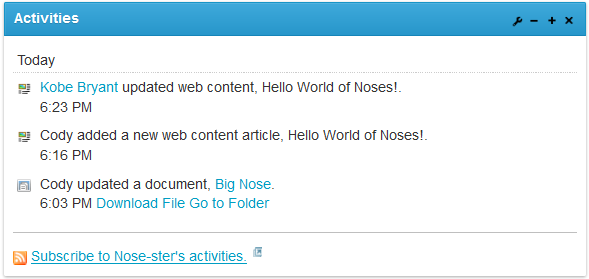
\includegraphics{../../images/01-social-activities.png}
\caption{\\Figure 1.7: Liferay Portal provides feeds of social activities.
These feeds can contain entries from any of Liferay's built-in
applications or applications that you write.}

\end{figure}

Social relationships within Liferay Portal are ideally suited for many
different kinds of implementations, whether you're building a public
social network or want to enable social features in your corporate
Intranet. Users can create relationships within the system, allowing
them to see updates from those whose activity they need to track. That's
far more powerful than having them subscribe to multiple individual RSS
feeds or visit multiple profiles, because the system keeps track of the
updates from those with whom you have a relationship, automatically.

More than this, however, Liferay is a great integration platform for
social applications. It fully supports the OpenSocial framework. You can
use Liferay Portal's built-in OpenSocial gadget editor to create and
serve your own OpenSocial gadgets.

\begin{figure}[htbp]
\centering
\scalegraphics{../../images/01-opensocial-gadget-editor.png}
\caption{Figure 1.8: Liferay Portal's OpenSocial gadget editor lets you
rapidly create social applications that can be served across the web to
any other OpenSocial container.}
\end{figure}

Liferay Portal also supports the creation of Facebook applications; in
fact, no additional coding is necessary to publish your Liferay
applications on Facebook (you would, of course, need to use Facebook's
API to use Facebook-specific features--such as posting on users'
timelines). The only thing you need to do is get an API key and canvas
page URL from Facebook.

\begin{figure}[htbp]
\centering
\scalegraphics{../../images/01-facebook-integration.png}
\caption{Figure 1.9: Any Liferay application can be published to
multiple social networks with a few clicks.}
\end{figure}

As you can see, Liferay Portal is built for social applications: adding
social features to your web site, creating a social network of your own,
creating social applications to be published on other web sites, or
building a social application for Facebook.

As with social applications, Liferay Portal is also an easy to use,
robust platform for any web application you're considering writing. In
addition to this, Liferay Portal is easily configured to be used as a
shared hosting platform for multiple web sites. Let's look at the
benefits you can reap by using Liferay Portal in these ways.

\section{Using Liferay as a web platform
}

We can't even begin to imagine what you're thinking of building, but
whatever it is, you're going to put your heart and soul into it.
Building it on Liferay's web platform can give you a leg up, by
providing to you everything you need to support your application, so you
can concentrate solely on what \emph{you're} building, and not the rest
of the features your users expect will come along with it.

\subsection{Liferay as an application development platform
}

Imagine your application for a moment. Does it require users to register
with your site? Will they be able to comment on content contained within
your application? Is there some asset that users can tag or categorize?
If you think about the layout of the application, would it benefit from
modularization? Could you make use of a rich JavaScript framework with
many components built into it? How about security--will you need to make
information available to some users, but not to all users? Liferay
Portal has all of this and more available to the developer, so you don't
have to write it yourself.

Liferay Portal's development framework is a great help when you're
building a web application. While the framework itself is covered in
other resources such as the \emph{Liferay Developer's Guide} or
\emph{Liferay in Action}, the strengths of Liferay as a platform are
also apparent once you've finished writing your application.

For example, bug fixes to your applications are easy to apply, because
Liferay applications are hot deployed to the running server. Liferay's
Marketplace gives you a ready-made shopping center for your
applications. And Liferay's web services and JSON architecture make it
easy for you to share data from your applications to other systems
running on different platforms.

You get all this--not to mention the automatic Facebook and OpenSocial
integration mentioned above--simply by using Liferay's development
platform. It's a very powerful platform, and certainly worth your
investigation.

\subsection{A great integration platform
}

If you're building an enterprise system, portals were designed in the
first place to be a single point of entry to your users' applications
and content. Since Liferay Portal integrates well with user directories
such as LDAP and Active Directory, and single sign-on systems such as
SAML and OpenSSO, it fits well into your enterprise systems. This allows
you to use it as an integration platform for existing applications.

Liferay Portal, since it adheres to the JSR standard for portlets, was
designed from the ground up for application integration. You can mix and
match any application installed in the system on any page within the
portal. You can make use of any APIs provided by other systems to
integrate their data into an application window in Liferay. And
applications you create with Liferay's Service Builder API are web
service-enabled from the start.

\subsection{Hosting multiple sites on Liferay Portal
}

Liferay Portal excels as a multi-site hosting platform. You can use it
to host multiple sites under the same overall architecture (like
Facebook, MySpace, or Pinterest offer to their users), or you could host
several completely different web sites based solely on Liferay's ability
to serve multiple instances of itself from the same physical
installation.

In the first scenario, Liferay Portal's Sites architecture lets you
create multiple, different web sites that have public and/or private
sets of pages and as many pages within those sets as you'd like. Users
join the web site, and once they're members, they can join and leave
open sites with one click. Some sites can be defined as restricted or
private, and users can't access those unless they're added by site
administrators. All of these sites can have canonical domain names such
as baseballcards.liferay.com or progrock.liferay.com.

Using this construct, you can build anything from Facebook, to Yahoo
Groups, to SourceForge, to the now-defunct-but-once-loved Geocities.
There is no limit to the number of sites you can have: some Liferay
installations have only one or two, but others have many thousands.

In the second scenario, Liferay Portal lets you create completely
separate instances of itself from the same installation. Users, groups,
organizations, sites, and roles from each instance are kept completely
separate. If a user registers for a user id on one instance, he or she
would have to register as a new user on another instance as well.

This lets you host many different, separate web sites from one Liferay
Portal installation. Users of each instance have access to the same
powerful content management, collaboration, social, and web development
platform that they'd have if they were operating from a single,
standalone installation.

\section{Extending and customizing Liferay for your own needs
}

Beyond using Liferay as a development platform for new applications,
Liferay Portal has also been designed to be extended and modified. As an
open source project, its source code is available, but Liferay Portal's
developers have designed the product to make it easy to build whatever
you want out of it.

Special software components called \emph{hook} and \emph{ext} plugins
enable developers to change any aspect of Liferay's interface and
behavior--without having to modify any of Liferay Portal's source code.
This provides you all the benefits of the ``build from scratch''
strategy we mentioned earlier, but without all the effort to build from
scratch. If you want to make a change to the user registration screens,
add support for a proprietary single sign-on mechanism that you've
written, revise the user interface for the message boards application,
or anything else, you can make those customizations. And if you're a
developer, we're sure you know that it's a whole lot easier to customize
something that \emph{almost} does things exactly the way you want than
it is to write that feature from scratch. With Liferay Portal, you
\emph{can} have your cake and eat it too.

\section{Summary }

So what is Liferay? As you can see, it's hard to describe, because it
does so much. What we've essentially done is say it's a totally awesome
content and document managing, user collaborating, socially enabling,
application developing, corporate integrating, completely customizable
platform for building the Internet. If we'd said that up front, you'd
probably have doubted us. Hopefully now, you can see that it's true.

If you're interested in using Liferay Portal for \emph{your} product,
continue reading. We'll go through all of these features (and more that
we couldn't mention) throughout the rest of the book.

\chapter{Web Content Management
}

Web Content Management is a system which allows non-technical users to
publish content to the web without having advanced knowledge of web
technology or programming of any sort. Liferay WCM empowers you to
publish your content with a simple point and click interface and it
helps you to keep your site fresh. You'll find yourself easily creating,
editing and publishing content within just a few minutes of being
exposed to its features. But Liferay WCM doesn't sacrifice power for
simplicity. If need be, you can use your developer skills to create
complex presentation layer templates that make your content ``pop'' with
dynamic elements. Once these templates have been deployed into the
portal, your non-technical users can manage content using these
templates as easily as they would manage static content. All of this
makes Liferay WCM an appropriate choice for sites with only a few pages
or sites with gigabytes of content.

In this chapter, we'll cover the following topics:

\begin{itemize}
\item
  Features of Liferay WCM
\item
  Creating sites and managing pages
\item
  Authoring content
\item
  Publishing content
\item
  Workflow
\item
  Site memberships and permissions
\end{itemize}

As you'll see, Liferay's WCM is a full-featured solution for managing
your web site. We'll start with an overview of what it has to offer and
then we'll dive down into its features. Note that web content is just
one kind of asset on Liferay. Other types of content (blog posts, wiki
articles, message board posts, etc.) are also considered assets. Liferay
provides a general framework for handling assets that includes tags,
categories, comments, ratings, and more. Please see chapter 5 for more
information on Liferay's asset framework.

\section{How Can Liferay's WCM Help You?
}

With Liferay's WCM you have the ability to create, edit, stage, publish
and approve content with easy to learn yet powerful tools. Liferay's WCM
streamlines the content creation process for end users. It's much faster
to use Liferay's WCM than it would be to create all the content for your
site in HTML. Some ways Liferay WCM makes this possible include:

\begin{itemize}
\item
  Once set up, non-technical users can manage the site.
\item
  Liferay's fine-grained permissions system ensures your content gets to
  the right users.
\item
  To manage the site, no programming is required.
\item
  Content can be staged.
\item
  Content can be passed through a workflow.
\item
  Content can be published on a schedule.
\item
  WCM is integrated with Liferay's services so advanced template
  developers can use them to query for data stored elsewhere in Liferay.
\end{itemize}

Once you get familiar with Liferay WCM you'll wonder how you ever got
along without it.

\subsection{What Features Does Liferay WCM Have?
}



Liferay's WCM has a host of features the makes managing the content of
your site easier.

\begin{itemize}
\item
  \textbf{WYSIWYG Editor:} A complete HTML editor that allow you to
  modify fonts, add color, insert images and much more.
\item
  \textbf{Structure Editor:} Easily add and remove fields you want
  available to content creators and then dynamically move them around.
  This editor includes an entire suite of form controls you can drag and
  drop onto your structure.
\item
  \textbf{Template Editor:} Import template script files that inform the
  system how to display the content within the fields determined by the
  structure.
\item
  \textbf{Web Content Display:} A portlet that allows you place web
  content on a page in your portal.
\item
  \textbf{Asset Publisher:} A portlet which can aggregate different
  types of content together in one view.
\item
  \textbf{Scheduler:} Lets you schedule when content is reviewed,
  displayed and removed.
\item
  \textbf{Workflow Integration:} Run your content through an approval or
  review process.
\item
  \textbf{Staging:} Use a separate staging server or stage your content
  locally so you can keep your changes separate from the live site.
\end{itemize}

Liferay's Web Content Management is a powerful and robust tool for
creating and organizing content on your web site. Let's begin by
examining some basic concepts involving sites and pages.

\section{Creating sites and managing pages
}

With most products, you would learn what the software can do in terms of
setting up your users and security model and then start building your
system. You'd design your infrastructure and get your server environment
up and running while your developers write the applications that live on
your web site. With Liferay Portal, however, you start farther ahead.
Liferay Portal is more than just a \emph{container} for applications
with a robust security model. It already includes many of the
applications you'll need, out of the box, ready to go and integrated
with all the user management and security features you've already
learned about.

Nearly all Liferay users use Liferay's Web Content Management system
(WCM). After all, all every web site has content that needs to be
managed. Liferay's WCM empowers you to manage all the content on your
site quickly and easily within your browser. Beyond managing existing
content, Liferay WCM lets users easily create and manage everything from
a simple article containing text and images to fully functional web
sites. Web publishing works alongside Liferay Portal's larger collection
of applications, which means you can add shopping cart functionality,
visitor polls, web forms, site collaboration tools and more. Everything
is done with our collection of easy-to-use tools with familiar rich-text
editors and an intuitive interface.

In this section we'll cover some basic aspects of Liferay WCM,
including:

\begin{itemize}
\item
  Page types
\item
  Layouts
\item
  Page and content permissions
\item
  Importing and exporting content
\item
  Content creation and editing
\item
  Content publishing
\item
  WCM Workflow
\end{itemize}

By the time we're done, you should be able to apply all these concepts
to your own content. To demonstrate Liferay's Content Management
features, we'll create and manage content on the portal for
\emph{Nose-ster}, a new social network where people are connected based
on what their noses look like.

First, a little housekeeping. If we're going to be \emph{Nose-ster}, our
portal should also be called Nose-ster. To set general information about
your portal like the name and mail domain, go to the Control Panel and
select \emph{Portal Settings} under the Portal heading. You could set up
the configuration for Nose-ster as follows.

\begin{figure}[htbp]
\centering
\scalegraphics{../../images/04-web-content-changing-settings.png}
\caption{Figure 2.1: Changing Portal Settings}
\end{figure}

You can also customize the logo in the top left corner of every page by
selecting \emph{Display Settings} under the \emph{Miscellaneous} tab on
the panel to the right. Once you've made the changes, we can begin
creating pages.

\subsection{Creating and managing pages
}

You have a few options for accessing the page creation interface. To
simplify this, we'll cover the Dockbar's \emph{Manage} menu slightly out
of order. There are two interfaces to be aware of: \emph{Site Pages} and
\emph{Page}. You can get to these from multiple places. Depending on
what you're editing and where you are on the portal, you'll use either
the \emph{Manage} menu or the Control Panel to work with your pages.
From the Control Panel, make sure you have the correct site selected in
the context menu selector and click the \emph{Site Pages} link in the
content section. If you've already navigated to the site you wish to
manage, click \emph{Manage} from the Dockbar and select \emph{Site
Pages}. This is the exact same interface you see in the Control Panel.
To manage the specific page of the site you've navigated to, click
\emph{Manage} and select \emph{Page}.

\begin{figure}[htbp]
\centering
\scalegraphics{../../images/04-web-content-managing-single-page.png}
\caption{Figure 2.2: Managing Individual Pages}
\end{figure}

For convenience, you can also navigate to the Sites page under the
Portal section of the Control Panel and click \emph{Actions} →
\emph{Manage Pages}. To quickly add a single page while to the site
you're browsing, click \emph{Add} from the Dockbar and select
\emph{Page}. Just enter a name for the page and it's added immediately.
Click the name of the page in the navigation menu to visit it and start
working on it.

\begin{figure}[htbp]
\centering
\scalegraphics{../../images/04-managing-site-pages.png}
\caption{Figure 2.3: Managing Site Pages}
\end{figure}

\emph{Site Pages} is an interface to view existing pages, create new
pages, view pages and export or import pages using Liferay Archive (LAR)
files. Note that you can switch between managing a set of pages and
managing a single page using the left-hand side navigation menu. Click
on \emph{Public Pages} or \emph{Private Pages} to manage the group or
click on an individual page to manage just that one. Switching views
like this changes the list of available tabs to the right. By default,
liferay.com, which we renamed to nosester.com, contains a single public
page called \emph{Welcome}.

Liferay's page groups are always associated with sites. Even users'
personal pages are part of their personal sites. All pages belong to one
of two types of page sets: public pages and private pages. By default,
public pages are accessible to anyone, even non-logged in users
(guests). Private pages are accessible only to users who are members of
the site which owns the pages. This means the private pages of an
organization's site would be viewable only by members of the
organization.

Regardless of whether the pages are public or private, Liferay uses the
same interface to manage them. Let's look at this interface more
closely.

\subsubsection{More page management tools
}

From the Manage Site Pages dialog box, you can add a page to the site by
clicking the \emph{Add Page} button. Because \emph{Public Pages} is
selected on the left, clicking \emph{Add Page} here adds a top level
page next to the Welcome page. You can, however, nest pages as deeply as
you like. To create a sub-page under the Welcome page, select the
\emph{Welcome} page first and then create your page. If you later decide
you don't like the order of your pages, you can drag and drop them in
the list to put them in whatever order you want. Let's go ahead and add
another top level page and name it \emph{Community}. We'll use this page
for the Recent Bloggers and Wiki portlets.

\begin{figure}[htbp]
\centering
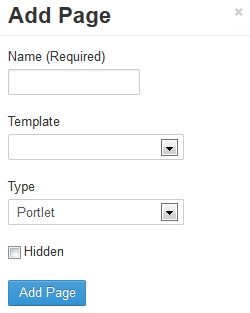
\includegraphics{../../images/04-web-content-add-page.png}
\caption{\\Figure 2.4: Adding Pages}
\end{figure}

When you create a new page, you can create either a blank page or a page
prepopulated with portlets from a page template. When you're entering
the name of the page, you can select from a list of page templates that
are currently available. To view the pages once you add them, click the
\emph{View Pages} button. This is how you'd populate your pages with
content and applications. This is covered in succeeding chapters.

If you're using the Manage Pages interface to create a new page, you'll
have some additional options to create different types of pages. There
are \textbf{Portlet Pages}, \textbf{Panel Pages}, \textbf{Embedded
Pages}, \textbf{URL Pages} and \textbf{Link to Page}. By default, all
pages are created as portlet pages but in some situations you might want
to use one of the other options.

\textbf{Portlet Pages} are the pages we're usually talking about. They
have a layout which you can drag and drop portlets into. Most of the
pages you create will be portlet pages.

\textbf{Panel Pages} can have any number of portlets on them, as
selected by an administrator, but only one will be displayed at a time.
Users select which portlet they want to use from a menu on the left side
of the page and the selected portlet takes up the entire page.

\begin{figure}[htbp]
\centering
\scalegraphics{../../images/web-content-panel-page.png}
\caption{Figure 2.5: A panel page}
\end{figure}

\textbf{Embedded Pages} display content from another website inside of
your portal. An administrator can set a URL from in the page management
interface and that page will appear in the context and within the
navigation of your Liferay portal.

\textbf{URL Pages} are just redirects to any URL specified by an
administrator. You can use URL pages to create links to pages belonging
to other sites of your portal or to pages of an external site. Use URL
pages cautiously since blind redirects create a poor user experience.

\textbf{Link to Page} creates a portal page which functions as an
immediate redirect to another page within the same site. You can select
which page to link to from a dropdown in the page management interface.
You could use a \emph{Link to Page} to place a deeply nested page in the
primary navigation menu of your site, for example.

Once you've created pages and populated them with content, Liferay
provides a way for you to back them up to separate files. Let's see how
that works.

\paragraph{Backing up and Restoring Pages
}



Next to the \emph{Add Page} button in the Manage Site Pages screen are
two buttons labeled \emph{Export} and \emph{Import}. The Export button
exports the pages you create into a single file, called a LAR (Liferay
Archive). You can then import this file into any server running Liferay
to re-create the pages. If you have a LAR you would like to import, use
the \emph{Import} button. Exporting and Importing LARs is a great way to
take content from one environment (say, a development or QA environment)
and move it all in one shot to your production server. Note that you
should not make this a regular occurrence. If you want to regularly move
pages from one server to another, you should use Liferay's staging
environment, which is covered in chapter 3.

LARs are also a good way to back up your site's content. You can export
them to a specific location on your server which is backed up, and if
you ever have to restore your site, all you need to do is import the
latest LAR file. One limitation on LAR files, however, is that they are
version dependent, so you can't use an export from an old version of
Liferay and import it into a newer version.

Let's be good administrators and export a LAR file for backup purposes.
Click on the \emph{Export} button and then name the file
\texttt{nosesterv1.lar}. Use the check boxes to determine what you'd
like to export. For this initial export, select everything. Note that if
you select the \emph{More Options} link, the list expands to include
data from many of Liferay's applications, including the Documents and
Media Library, Message Boards and Web Content. You can also export the
theme you're using.

Once you click \emph{Export}, your browser prompts you to save the file.
Once you have the file, you can copy it to a backup location for
safekeeping or import it into another installation of Liferay Portal. If
you must rebuild or wish to revert back to this version of your site,
you can import this file by clicking the \emph{Import} button from the
Manage Site Pages dialog box, browsing to it and selecting it.

Next, we'll look at the options on the right side menu, starting with
Look and Feel.

\paragraph{Customizing the Look and Feel
}



When you open the Manage Site Pages dialog box it defaults to the Look
and Feel tab. On this tab, you're presented with an interface that
allows you to choose a theme for the current site. Themes can transform
the entire look of the portal. They are created by developers and are
easily installed using the Liferay Marketplace. Since we don't have any
themes beyond the default one installed yet, we'll use the default theme
for our pages.

\begin{figure}[htbp]
\centering
\scalegraphics{../../images/04-look-and-feel.png}
\caption{\\Figure 2.6: Look and Feel Interface}
\end{figure}

Many themes include more than one color scheme. This allows you to keep
the existing look and feel while giving your site a different flavor.
Change the color scheme from blue to green by selecting \emph{Green}
under \emph{Color Schemes}. If you now go back to the site (by clicking
\emph{Back to nosester.com} in the top left corner of the Control
Panel), you'll see some parts of the page are now tinged in a greenish
hue.

If you apply a color scheme to a set of public or private pages it is,
by default, applied to each page in the set. If, however, you open the
Manage Pages dialog box for a particular page, you can select
\emph{Define a specific look and feel for this page} to make the color
scheme apply to this page only. You can use this feature to choose a
different color scheme for a particular page than the one defined for
the set of public or private pages to which it belongs.

There are a few more configurable settings for your theme. You can
switch the bullet style between dots and arrows and you can choose
whether or not to show portlet borders by default.

Also notice themes can apply to regular browsers or mobile devices. You
could create another site for mobile users attached to the
\href{http://m.nosester.com}{http://m.nosester.com} address and serve up
a page designed for the smaller screens on phones.

The \emph{CSS} section allows you to enter custom CSS that will also be
served up by your theme. In this way, you can tweak a theme in real time
by adding new styles or overriding existing ones.

The next option configures the logo that appears for your site.

\paragraph{Using a custom logo
}

If you want to use your own logo for a specific site, use the Logo tab.
Adding a custom logo is easy: select the Logo tab and browse to the
location of your logo. Make sure your logo fits the space in the top
left corner of the theme you're using for your web site. If you don't,
you could wind up with a site that's difficult to navigate, as other
page elements are pushed aside to make way for the logo.

In the logo tab, you can also choose whether or not to display the site
name on the site. If you check the box labeled \emph{Show Site Name} the
site name will appear in the the top right corner of the page. This
option is enabled by default and cannot be disabled if the \emph{Allow
Site Administrators to set their own logo} option is disabled in
\emph{Portal Settings}. It is also not available for the default site --
only newly created sites and user pages have the option to have the name
display.

\subsubsection{Changing options for individual pages
}



When you select a single page, some different options appear. Let's look
at what these do.

\textbf{Details:} lets you name the page for any localizations you need.
You can also set the HTML title that appears in the browser window for
the page. Plus you can set an easy to remember, friendly URL for the
page.

\textbf{SEO:} provides several means of optimizing the data the page
provides to an indexer that's crawling the page. You can set the various
meta tags for description, keywords and robots. There's also a separate
Robots section that lets you tell indexing robots how frequently the
page is updated and how it should be prioritized. If the page is
localized, you can select a box to make Liferay generate canonical links
by language. If you want to set some of these settings for the entire
site, you can specify them from the Sitemaps and Robots tabs of the
Manage Site Settings dialog box (see below).

\begin{roundedframe}
  \begin{wrapfigure}{l}{0.12\textwidth}
      
\includegraphics{../../images/01-tip.png}
  \end{wrapfigure}
In previous versions of Liferay, it was possible that a single page could be indexed multiple times. In Liferay 6.1, all URLs that direct to the same page will only
create one entry in the index. Previously, the simple URL
\emph{http://www.nosester.com/web/guest/blog/-/blogs/thenose} and
different versions of the URL which provided additional information
about the referring page had different entries in the index. As of
Liferay 6.1, each asset (web content article, blog entry, etc.) has a
unique URL. From the search engine's point of view, this will make your
pages rank higher since any references to variations of a specific URL
will all be considered references to the same page.
\end{roundedframe}

\textbf{Look and Feel:} lets you set a page-specific theme.

\textbf{Layout:} lets you specify how portlets are arranged on a page.
Choose from the available installed templates to modify the layout. It's
very easy for developers to define custom layouts and add them to the
list. This is covered more thoroughly in both the \emph{Liferay
Developer's Guide} and in \href{http://manning.com/sezov}{\emph{Liferay
in Action}}.

\textbf{JavaScript:} gives you the ability to paste custom JavaScript
code to be executed on this page.

\textbf{Custom fields:} If custom fields have been defined for pages
(which can be done from the \emph{Custom Fields} page of the Control
Panel), they appear here. These are metadata about the page and can be
anything you like, such as author or creation date.

\textbf{Advanced:} contains several optional features. You can set a
query string to provide parameters to the page. This can become useful
to web content templates, which you'll see in the next chapter. You can
set a target for the page so that it either pops up in a particularly
named window or appears in a frameset. And you can set an icon for the
page that appears in the navigation menu.

\textbf{Mobile Rule Groups:} allows you to apply rules for how this page
should be rendered for various mobile devices. You can set these up in
the \emph{Mobile Device Rules} section of the Control Panel.

\textbf{Customization Settings:} lets you mark specific sections of the
page you want users to be able to customize.

Note that the \emph{Manage → Page Layout} menu directs you to the same
Layout tab that's in \emph{Manage → Page}.

\subsubsection{Modifying Page Layouts
}

Page layouts allow you to arrange your pages so the content appears the
way you want it to. Liferay comes with many layouts already defined.
Developers can create more and they can be deployed to your portal for
your use.

To prepare for the portlets we'll soon be adding, let's change the
layout of the Collaboration page. To access layouts, select \emph{Manage
→ Page Layout} from the Dockbar.

Now, select the \emph{2 Columns (70/30)} layout and click \emph{Save}.
Once saved, you'll return to the page and it'll seem as though nothing
has happened. Once we start adding portlets, however, you'll notice the
page is now equally divided into two columns. You can stack portlets on
top of each other in these columns. There are, of course, more
complicated layouts available and you can play around with them to get
the layout you want.

Sometimes a particular layout is \emph{almost} what you want but not
quite. In this case use the Nested Portlets portlet to embed a layout
inside another layout. This portlet is a container for other portlets.
It lets you select from any of the layouts installed in Liferay, just
like the layouts for a page. This gives you virtually unlimited options
for laying out your pages.

The next option in the \emph{Manage} menu is page customizations.

\subsubsection{Page Customizations
}

Page Customizations are a new feature in Liferay 6.1. With page
customizations, any user with the appropriate permissions can create
personalized versions of any public page. Before users can create
personalized versions of pages, customizations must first be enabled by
an administrator. Administrators can activate or deactivate
customizations for any row or column on any page. When users customize a
page, they have the option to use either their version or the default
version of a page. Users can't see alternate versions of pages other
than their own.

\begin{figure}[htbp]
\centering
\scalegraphics{../../images/04-web-content-personal-customization.png}
\caption{Figure 2.7: Setting Customizable Columns}
\end{figure}

When an administrator activates page customizations for a page, any
portlets that are in a \emph{Customizable} row or column can be moved
around the page or removed from the page. Users can add new portlets of
their own choosing to these columns of the page and can also customize
portlet configurations. If at any time users determine they don't like
their customizations, they can click \emph{Reset My Customizations} to
revert their pages back to the default. For more information about page
customizations, please refer to the Page Customizations section of
chapter 6.

Now that you know how to enable page customizations, let's look at the
settings for the site as a whole.

\subsubsection{Configuring Site Settings
}

As with Site Pages, you can access Site Settings through the Control
Panel or directly from the site using the Dockbar (\emph{Manage} →
\emph{Site Settings}).

\begin{figure}[htbp]
\centering
\scalegraphics{../../images/web-content-site-settings.png}
\caption{Figure 2.8: Site Settings}
\end{figure}

You'll find options to specify details and metadata about your site, set
up friendly URLs and virtual hosts, configure search engine optimization
settings, turn staging on or off and specify a Google Analytics ID.
Let's take a closer look.

\textbf{Details:} allows an administrator to change the description and
membership type of a site and also to specify tags and categories for
the site. The membership type can be set as open, restricted or private
based on the privacy needs of the site. Users can join and leave an open
site at will. To join a restricted site, a user has to be added by the
site administrator. A user can also request to be added through the
Sites section of the Control Panel. A private site is like a restricted
site but doesn't appear in the Sites section of the Control Panel for
users who aren't members.

\textbf{Pages:} From Site Settings, click on \emph{Pages} to manage some
basic features of the pages on a site. If no pages have been defined
yet, you can set site templates for the public or private pages. If
pages already exist, links are provided to view them. You can also
change the site's application adapter, which is a special type of hook
plugin that customizes out of the box functionality for specific sites.

\textbf{Site URL:} Set a friendly URL and/or a virtual host for your
site here. The \emph{Friendly URL} option lets you manage the path to
your site in the portal's URL. Friendly URLs are used for both public
and private pages. For public pages, the friendly URL is appended to
http://localhost:8080/web. For private pages, the friendly URL is
appended to http://localhost:8080/group. Each friendly URL needs to be a
unique name, of course. Having a human-readable friendly URL assists
indexing bots and is critical to good search engine optimization.

For example, suppose you were creating a portal for a bank called the
Best Bank. If you set the friendly URL of your portal's default site to
/best-bank, the URL of your default site's public home page would change
to http://localhost:8080/web/best-bank/home. If your portal's default
site had private pages, the URL of the default private home page would
change to http://localhost:8080/group/best-bank/home.

Note that if you're adding a friendly URL for your portal's home page,
you should update your portal's Home URL field so that page requests to
http://localhost:8080 redirect properly. To do this, navigate to the
Portal Settings page of the Control Panel and find the Home URL field in
the Navigation section. For our bank example, we would enter
\emph{/web/best-bank/home} into the Home URL field. Once you've entered
this setting, page requests to localhost:8080 will redirect to the
friendly URL of your portal's new homepage:
http://localhost:8080/web/best-bank/home.

\emph{Virtual Hosts} make web navigation much easier for your users by
connecting a domain name to a site. This tab allows you to define a
domain name (i.e., www.mycompany.com) for your site. This can be a full
domain or a subdomain. This enables you to host a number of web sites as
separate sites on one Liferay server.

For instance, if we set this up for Nose-ster's Development Network,
users in that site could use developers.nosester.com to get to their
site, provided Nose-ster's network administrators created the domain
name and pointed it to the Liferay server.

To set this up, the DNS name \emph{developers.nosester.com} should point
to your portal's IP address first. Then enter
\emph{http://developers.noseter.com} in the Virtual Host tab for the
Developers site. This helps users quickly access their site without
having to recall an extended URL.

\textbf{Site Template:} If you've created the site from a site template,
this section displays information about the link between the site
template and the site. Specifically, you can see which site template was
used and whether or not it allows modifications to the pages inherited
from it by site administrators. If you're not using site templates for
this site, you can safely ignore this section.

\textbf{Sitemap:} lets you send a sitemap to some search engines so they
can crawl your site. It uses the sitemap protocol, which is an industry
standard. You can publish your site to Yahoo or Google and their web
crawlers will use the sitemap to index your site. Liferay Portal makes
this very simple for administrators by generating the sitemap XML for
all public web sites.

By selecting one of the search engine links, the sitemap will be sent to
them. It's only necessary to do this once per site. The search engine
crawler will periodically crawl the sitemap once you've made the initial
request.

If you're interested in seeing what is being sent to the search engines,
select the \emph{Preview} link to see the generated XML.

\textbf{Robots:} If you're using virtual hosting for this site, you can
configure \texttt{robots.txt} rules for the domain. The Robots page
gives you the option to configure your \texttt{robots.txt} for both
public and private pages on a site. If you don't have Virtual Hosting
set up, this tab is rather boring.

\textbf{Staging:} enables you to edit and revise a page behind the
scenes, then publish changes to your site once they have been completed
and reviewed. For a full explanation of Staging, see chapter 3: Advanced
web content management.

\textbf{Analytics:} allows you to integrate your pages with Google
Analytics. Liferay provides seamless integration with Google Analytics,
allowing you to place your ID in one place, then it will get inserted on
every page. This enables you to focus your efforts on building the page,
rather than remembering to put the code everywhere. Google Analytics is
a free service which lets you do all kinds of traffic analysis on your
site so you can see who visits, where visitors are from and what pages
they most often visit. This helps you tweak your site so you can provide
the most relevant content to your users.

Now that you know how to configure sites, let's look at page templates
and site templates.

\subsubsection{Page Templates and Site Templates
}



\emph{Page Templates} and \emph{Site Templates} are invaluable tools for
building similar pages on larger portals. As you continue to add pages
to sites in your portal, you'll notice repeatable patterns in the
designs of those pages. Page templates enable you to preconfigure a
single page and then apply it to any new page you create. Site Templates
allow you to do the same thing but on the scale of a site--if you have
multiple sites that use a similar structure of pages, you can create a
single site template and use it to create as many sites as desired. For
a full explanation of Page Templates and Site Templates, see chapter 3.

\subsubsection{Site Content }

Liferay 6.1 makes it easier to access Web Content management without
using the Control Panel. You can now click \emph{Manage} and then
\emph{Site Content} to access the same Web Content controls featured in
the Control Panel right from your portal page.

\begin{figure}[htbp]
\centering
\scalegraphics{../../images/web-content-site-content.png}
\caption{Figure 2.9: Site Content}
\end{figure}

You can manage the following kinds of content:

\begin{itemize}
\item
  Recent Content
\item
  Web Content
\item
  Documents and Media
\item
  Bookmarks
\item
  Calendar
\item
  Message Boards
\item
  Blogs
\item
  Wiki
\item
  Polls
\item
  Software Catalog
\item
  Tags
\item
  Categories
\item
  Social Equity
\item
  Dynamic Data Lists
\end{itemize}

For details about Liferay's social collaboration suite, see chapter 10.

\subsection{Creating the Nose-ster pages
}

There are a lot of other things you can do beyond placing portlets on a
page. So let's start working on the Nose-ster site. You can do this by
going up to the Dockbar and clicking \emph{Go to → Nose-ster}.

We'll use the \emph{Community} page you created earlier in the chapter.
Navigate to the \emph{Community} page and select \emph{Manage → Page}
from the Dockbar.

This screen should now be familiar to you but let's recap.

The Page tab allows you to:

\begin{itemize}
\item
  Change the name of the page
\item
  Enter HTML code for the title
\item
  Choose the page type
\item
  Hide the page from the theme navigation
\item
  Define a friendly URL to the page
\item
  Choose an icon to be displayed
\item
  Choose a frame target for the page
\item
  Copy an existing page
\end{itemize}

You can also enter custom meta tags or JavaScript to the page if you're
a web developer. Additionally, if you click the \emph{Permissions}
button, you can define which users, groups, roles or organizations can
view or edit the page.

The Children tab lets you create child pages underneath the page you've
selected. You can nest pages as deep as you like but for every page
below the top level hierarchy you must provide navigation to it via a
Navigation or Breadcrumb portlet, at least with most themes (including
the default). Developers can create themes which have cascading menu
bars which show the full hierarchy. Some examples of that are in
Liferay's plugin repositories.

For now, click \emph{Return to full page}. You should be able to define
and manage pages in Liferay at this point so let's look at what you'd
put on a page.

\subsubsection{Portlets }

As we discussed earlier, Liferay Portal pages are composed of portlets.
All of your site's functionality, from blogs to shopping, is composed of
portlets.

Adding portlets to a page is simple. Let's add some to our Collaboration
page.

\begin{enumerate}[1.]
\item
  In the Dockbar, select \emph{Add → More}.
\item
  In the menu that appears, expand the \emph{Collaboration} category.
\item
  Drag the \emph{Blogs Aggregator} portlet off the Add Application
  window onto the right column of our page.
\item
  Next, drag the \emph{Wiki} portlet to the \emph{left column}.
\end{enumerate}

See how easy it is to add applications to your pages? We've gone one
step further: we've got the Wiki portlet, the Blogs Aggregator portlet
and then a nested portlet with a different layout and the Alerts, Search
and Dictionary portlets in the figure below.

\begin{figure}[htbp]
\centering
\scalegraphics{../../images/04-web-content-portlet-layout.png}
\caption{Figure 2.10: Yeah, we're showoffs. But as you can see, your
page layout options are virtually limitless.}
\end{figure}

You'll find it's easy to make your pages look exactly the way you want
them to. If the layout options provided aren't enough, you can even
develop your own. More information about that can be found in Liferay's
official guide to development,
\href{http://manning.com/sezov}{\emph{Liferay in Action}}.

\subsubsection{Page Permissions
}

By default, public pages are just that: public. They can be viewed by
anybody, logged in or not logged in. And private pages are really only
private from non-members of the site. If someone has joined your site or
is a member of your organization, that person can see all the private
pages. You can, however, modify the permissions on individual pages in
either page group so only certain users can view them.

Let's say we wanted to create a page only for administrators to see. We
can do this with the following procedure:

\begin{enumerate}[1.]
\item
  Go to the Dockbar and select \emph{Manage → Control Panel}.
\item
  Ensure you've selected the default site in the context selector.
\item
  Click the \emph{Site Pages} link.
\item
  Click the \emph{Private Pages} tab to switch to the Private Pages.
  Remember, these pages by default are viewable only by members of the
  site.
\item
  Create a page called \emph{Admin Tips}.
\item
  Click on the page in the tree on the left and then click
  \emph{Permissions}.
\item
  Uncheck the \emph{View} and \emph{Add Discussion} permissions next to
  the Site Member role.
\item
  Click the \emph{Save} button.
\end{enumerate}

\begin{figure}[htbp]
\centering
\scalegraphics{../../images/04-web-content-page-permissions.png}
\caption{Figure 2.11: Permissions for Admin Tips}
\end{figure}

Congratulations! You've just changed the permissions for this page so
only site administrators can view it. Any users you add to this role can
now see the page. Other users, even members of this site, won't have
permission to see it.

Pages in Liferay are as flexible as pages you'd create manually without
a portal. Using a point and click interface, you can define your site
any way you want. You can create and remove pages, export and import
them, set their layouts, define how they are indexed by search engines
and more. You've also been introduced to Liferay's concept of sites.
Again, using a point and click interface, you can create multiple web
sites and define how users can access them, whether they are linked to a
domain name and create all of their pages.

You now understand how to manage pages in Liferay Portal. It's time to
move on to adding content to those pages. Liferay's Web Content
Management (WCM) is a highly powerful, yet flexible, set of tools that
enables you to successfully manage your web site.

You'll soon discover that Liferay's WCM is easy to learn and highly
configurable. If you already have experience with WCM, you'll see some
new features and improvements to old ones. If you're new to Liferay's
WCM, then you'll be surprised at how fast you will be adding, editing
and scheduling content on your site. Once you're familiar with portlets
such as Web Content Display and Asset Publisher, your ability to manage
an immense site with a large amount of content will simply amaze you.

We'll be using Liferay's WCM to publish simple pieces of content,
develop templates to define how content is to be displayed, set up a
workflow for content to be approved, schedule when content is to be
published and much, much more.

\section{Authoring (basic) content
}

You've been assigned the task to build a web site for an innovative new
social networking site called Nose-ster. You've decided to take
advantage of Liferay Portal and its rapid deployment features as well as
its ability to get a fully functional, content-rich web site with
integrated social features up and running in little time. Together, we
can get you started.

We'll walk through the creation of Nose-ster's web site, starting by
creating and publishing some simple content using Liferay's built-in
WYSIWYG editor. We'll then take advantage of Liferay's robust structure
editor. We'll use templates to display the content and then explore some
of the advanced publishing features such as the built-in workflow and
Asset Publisher.

\subsection{Creating content the simple way
}



As we've stated above, content is the reason web sites exist. Liferay
Portal has made it easier than ever to get content published to your
site. Because Liferay Portal is so flexible, you can use basic authoring
tools right away or take advantage of the more advanced features. It's
adaptable to your needs.

We'll begin by creating simple content using Liferay's WYSIWYG Editor
and then we'll publish it to the home page of Nose-ster's web site. This
is a fast and straightforward process that demonstrates how easy it is
to create and publish content on your Liferay Portal instance. Let's
learn about the Web Content section of the control panel so we can
create and publish our first pieces of content.

\begin{figure}[htbp]
\centering
\scalegraphics{../../images/04-web-content-context-dropdown.png}
\caption{\\Figure 2.12: Choosing a Site in the Content Section}
\end{figure}

When you manage web content from the Control Panel you can select the
location where the content resides. For instance, you can add content
that's available to a specific site or globally across the portal. The
Content section of the Control Panel displays as its heading the name of
the site you're currently working on. This heading is called the
\emph{context menu selector}: you can change the scope of where you'd
like to view, edit or create content by using the drop-down selector
attached to the heading.

\subsection{Rich, WYSIWYG Editing
}

Once you have the Nose-ster site selected, click on the \emph{Web
Content} link in the Control Panel. Next, click the \emph{Add} button
under the \emph{Web Content} tab. This is a highly customizable form
that by default has two fields: a title and a powerful WYSIWYG editor.
We could customize this form to contain whatever fields our content
needs but let's keep things simple for now. We'll cover more advanced
features such as structures, templates and content scheduling later in
this chapter.

For now, type the words \emph{Welcome to Nose-ster} in the \emph{Name}
field. Notice that content can be localized in whatever language you
want. If you click on the \emph{localize} checkbox, two select boxes
appear which allow you to pick the language you're working in and the
default language. You can enter translations of your content for any
language in the list. The screenshot below shows this interface but for
now, we won't be using it, so you can leave it unchecked. In the content
field, add a short sentence announcing the web site is up and running.

\begin{figure}[htbp]
\centering
\scalegraphics{../../images/04-web-content-wysiwyg.png}
\caption{Figure 2.13: The Web Content Editor provides many options for
customization.}
\end{figure}

Getting a new web site up and running is an exciting step for anyone,
whether it is a large corporation or a small non-profit charity. To
celebrate this momentous achievement at Nose-ster, let's give our
announcement some of the pomp and circumstance we think it deserves!

Using the editor, select all the text and then change the style to
\emph{Heading 1} and the color to \emph{Dark Green}.

You could insert an image here or even more text with a different style,
as demonstrated in the screenshot below. You can also add bullets,
numbering, links to another site or custom images. You can even add an
emoticon. Let's add a smiley face at the end of our announcement.

\begin{figure}[htbp]
\centering
\scalegraphics{../../images/04-web-content-example2.png}
\caption{Figure 2.14: View your content changes directly in the editor.}
\end{figure}

The WYSIWYG editor is a flexible tool that gives you the ability to add
text, images, tables, links and more. Additionally, you can modify the
display to match the purpose of the content. Plus it's integrated with
the rest of Liferay Portal: for example, when you upload an image to be
added to a page, that image can be viewed and manipulated in the
Documents and Media portlet.

If you're HTML savvy, Liferay WCM doesn't leave you out in the cold. You
can click the \emph{Source} button and write your own HTML if you wish.

On the right of the New Web Content form are options that allow you to
customize your web content.

\begin{figure}[htbp]
\centering
\scalegraphics{../../images/wcm-abstract.png}
\caption{Figure 2.15: New web content can be customized in various ways
using the menu on the right.}
\end{figure}

\textbf{Abstract:} lets you to create a brief summary of the web
content. You can also pair the text with a small image.

\textbf{Categorization:} specifies the content type from a list of
options. They are \emph{Announcements}, \emph{Blogs}, \emph{General},
\emph{News}, \emph{Press Release}, and \emph{Test}. You can also create
tags to make the content easier to find in a search. Note that these
categories are defined by a property in the properties file; see the
\texttt{journal.article.types} property in chapter 20 for further
information.

\textbf{Schedule:} customizes the date and time your content publishes
and/or expires.

\textbf{Display Page:} lets you determine where the web contents are
displayed when linked from other pages. The concept of the Canonical URL
is new to Liferay 6.1. The Canonical URL is unique for articles that
redirect the visitor to the article's default display page.

Imagine you have a newspaper with a sports section and a technology
section. You add a Sports page and a Tech page to your site, each one
with a specific banner and look and feel. You want the articles to
appear in the appropriate pages, but you know in Liferay articles are
not related to pages. You can add an article as often as you like in
different web content display portlets or in configured Asset
Publishers. But if you have a \emph{View in context} link, where will
you show your article? This is where you'd use a default display page.
Articles that have a default display page defined are shown with other
related articles in the same display page.

Imagine you have 100 sports articles and 100 tech articles. In previous
versions of Liferay you'd need to create a page for each article to show
it. Now with only one sports page and one tech page, you can show all
articles in one place in a consistent fashion.

\paragraph{Creating a display page
}

There are two ways of creating a display page. You can use a
\emph{Content Display Page} template, which automatically creates
everything you need, or you can create one manually. The Content Display
Page template is found under \emph{Page Templates} in the Portal section
of the Control Panel.

To create a display page manually, add an Asset Publisher to a page.
Then make it the Default Asset Publisher for the page. This defines this
Asset Publisher as the one that displays the content if several Asset
Publishers are on the same page. Set this up by clicking
\emph{Configuration} on your Asset Publisher. Under the \emph{Setup}
tab, navigate to \emph{Display Settings} and check the checkbox labeled
\emph{Set as the Default Asset Publisher for This Page}.

Once you've given an article its default display page, links to the
article redirect the user to its default display page. To see how this
works, add an Asset Publisher to another page, like the Home page of the
newspaper, and configure it to \emph{View in a Specific Portlet}. This
setting is found in the \emph{Asset Link Behavior} menu under Display
Settings. If you click on the link, you'll be redirected to the Default
Display Page of the article.

You now see that the link looks something like this:

www.nosester.com/nose-article

This is an example of a canonical URL, and it's a nice enhancement for
Search Engine Optimization (SEO) because the article's URL becomes the
page URL. To a search engine that's crawling your site, this means that
the location of your article never changes. And if you decide to use the
content on another page in the future, the article is still available at
this URL. This feature is used in search results, in related assets and
in Asset Publishers. For more information on Liferay's Display Pages,
see chapter 5.

\textbf{Related Assets:} enables you to connect any number of assets
within a site or across the portal, even if they don't share any tags
and aren't in the same category. You can connect your content to a Blogs
Entry, Message Boards Message, Web Content, Calendar Event, Bookmarks
Entry, Documents and Media Document, and a Wiki Page.

\begin{figure}[htbp]
\centering
\scalegraphics{../../images/related-assets-link.png}
\caption{Figure 2.16: This blog entry has links to three Related Assets:
one web content display and two blog entries.}
\end{figure}

You'll learn how to publish links to related assets using the Related
Assets portlet in the \emph{Defining content relationships} section of
chapter 5.

\textbf{Permissions:} customize who has access to the content. By
default, content is viewable by Anyone (Guest Role). You can limit
viewable permissions by selecting any Role from the drop-down or in the
list. Additionally, Liferay Portal provides the ability to customize
permissions in more detail. Select the \emph{More Options} link next to
the drop down button and you'll find the different activities you can
grant or deny to your web content.

\begin{figure}[htbp]
\centering
\scalegraphics{../../images/04-web-content-content-permissions.png}
\caption{Figure 2.17: Permissions for Web Content allow you to fine-tune
how your content is accessed.}
\end{figure}

\textbf{Custom fields:} customize metadata about the web content. The
fields can represent anything you like, such as the web content's author
or creation date. If custom fields have been defined for web content
(which can be done from the \emph{Custom Fields} page of the Control
Panel), they appear here.

For more information on Custom Fields see the Custom Fields section in
chapter 16.

For this piece of web content, we don't need to change anything. After
you're finished with permissions, click \emph{Save as Draft}. This saves
the content in draft form. Once you're satisfied with your changes,
select \emph{Publish}. This makes the content available for display, but
we still have some work to do to enable users to see it. In Liferay WCM,
all content resides in a container, which is one of two portlets: Web
Content Display or Web Content List. By far the most frequently used is
the \emph{Web Content Display} portlet. Let's look at how it works.

\section{Publishing (basic) content
}



Now that we've created and published our first piece of web content for
Nose-ster, it's time to display it. First, add the \emph{Web Content
Display} portlet to our Welcome page by selecting \emph{Add → Web
Content Display} from the Dockbar.

\begin{figure}[htbp]
\centering
\scalegraphics{../../images/add-web-content-display.png}
\caption{\\Figure 2.18: Adding the Web Content Display Portlet}
\end{figure}

Once the portlet appears, drag it to the position on the page where you
want your content to appear. You can have as many Web Content Display
portlets on a page as you need, which gives you the power to lay out
your content exactly the way you want it.

To add existing web content, select the \emph{gear} icon on the lower
left of the portlet. You will see the message \emph{Please select a web
content from the list below}. You have several options here.

Naturally, if your content appears in the list, you can simply select
it. If there is lots of published content available, you could search
for the content by name, ID, type, version, content and site (click the
\emph{Advanced} link to see all the options). You can also show the
available locales for your content. If you're working on the page for a
particular language, you can select the translation of your content that
goes with your locale.

\begin{figure}[htbp]
\centering
\scalegraphics{../../images/04-web-content-choosing-web-content.png}
\caption{Figure 2.19: Publishing web content is a snap. At a minimum,
you only have to select the content you wish to publish. You can also
enable lots of optional features to let your users interact with your
content.}
\end{figure}

If you have enabled OpenOffice.org integration with your portal, you can
also enable document conversion for your content. This gives your users
the ability to download your content in their format of choice. This is
especially handy if you are running a research or academically oriented
site; users can very quickly download PDFs of your content for their
research projects.

Note that you also have other options, such as enabling a Print button,
enabling ratings so users can rate the content, enabling comments and
enabling ratings on comments.

The Print button pops the content up in a separate browser window that
contains just the content, without any of the web site navigation. This
is handy for printing the content. Enabling ratings shows one of two
ratings interfaces Liferay has: five stars or thumbs up and thumbs down.
This can be set globally in the \texttt{portal-ext.properties} file. See
chapter 12 for further information about this.

Enabling comments creates a discussion forum attached to your content
which users can use to discuss your content. Enabling ratings on
comments gives your users the ability to rate the comments. You may
decide you want one, some or none of these features, which is why
they're all implemented as simple check boxes to be enabled or disabled
at need.

If you click the \emph{Supported Clients} tab, you'll see you can choose
the type of client to which you want to expose content. This lets you
target the large screens of users' computers for expansive graphics and
lots of special effects or target the small screens of mobile devices
with pertinent information and a lightweight page. For now, leave both
checked and click the \emph{Save} button. You can now close the
configuration window.

To publish new content, select the \emph{page and green plus icon} on
the lower left of the portlet. This launches the same full-featured
editor you've already seen in the Control Panel, which lets you add and
edit content in place as you are working on your page.

This is another example of the flexibility that Liferay Portal offers.
At times, you may want to add content directly into the Web Content
Display portlet of the page you're managing, especially if you are in
the process of building the page. At other times, you may want to use
the Control Panel to create content, because at that moment you're more
concerned with the creation of the content and not where the content
will later be displayed. Liferay WCM supports both processes.

Editing content that's already been published is just as easy as
creating new content is. You'll use the same exact tools.

\paragraph{Editing Content }

Once the content is displayed--whether you've selected content or
created it in the Web Content Display portlet--you can edit the content
directly from the Web Content Display portlet or from the Control Panel.
To edit it from the Web Content Display portlet, select the
\emph{pencil} icon to the lower left of the portlet. This launches the
WYSIWYG editor and from there you can make any necessary changes.

\begin{figure}[htbp]
\centering
\scalegraphics{../../images/web-content-display-icons.png}
\caption{\\Figure 2.20: Edit, Select and Add Icons of Web Content Display
Portlet}
\end{figure}

When you publish your content this way, it becomes available immediately
(unless, of course, you have a workflow enabled, which we'll see below).
This happens whether you edit it in place or in the Control Panel.

Note: if you want to view your page the way your users will see it
(i.e., without all those portlet controls and icons), go up to the
Dockbar and select \emph{Toggle Edit Controls}. This makes all those
extra controls you see as a portal administrator disappear. If you need
to use those controls again, just select \emph{Toggle Edit Controls}
again.

That's pretty much all there is to simple content creation. Whole sites
have been created this way. But if you want to take advantage of the
full power of Liferay's WCM, you'll want to use structures and templates
found in chapter 3. Next, let's see how you can manage your content with
an approval process called workflow.

\section{Using Liferay's workflow with WCM
}



Workflow is essentially a predetermined sequence of connected steps. In
Liferay WCM, workflow is designed to manage the creation, modification
and publication of web content. You can set up a workflow so content
can't be published without going through an approval process you design.
In this way, content is published to the site only after it has been
reviewed and approved.

Liferay's workflow engine is called Kaleo workflow and it ships with
Liferay CE. If you have uninstalled it or are using EE, it needs to be
installed and configured separately. This is covered in chapter 6. Since
we have somewhat of a ``What came first--the chicken or the egg?''
problem, for now, we'll assume it's installed and look at how you can
take advantage of workflow in getting your content through any approval
steps between creation and publication.

You may have noticed something appears to be missing from the staging
process discussed above. In particular, you might be asking the
question, ``How do I reject changes?'' Starting with Liferay 6.1,
Staging is integrated with Liferay's Workflow engine. To have a review
process for staged pages, you need to make sure you have a workflow
engine configured and you have staging set up in the workflow. To do
this, select the workflow definition desired for page revisions in the
Workflow Configuration.

When using a workflow, clicking \emph{Submit for Publication} submits
the staged pages into the workflow. Once all necessary approvals have
been completed, the page status is marked as ready for publication. The
\emph{Publish to Live Now} and \emph{Schedule for Publication} options
publish the last version of the selected pages marked as ready for
publication.

To enable workflow for Web Content, navigate to the Control Panel and
select \emph{Workflow Configuration}. From there, select a workflow that
has been deployed to Liferay.

\begin{figure}[htbp]
\centering
\scalegraphics{../../images/04-web-content-workflow-config.png}
\caption{Figure 2.21: Enabling Workflow for Content Management}
\end{figure}

As you'll discover in chapter 10, you can design workflows to suit your
organization's approval process. For Nose-ster's implementation we'll
use the \emph{Single Approver} workflow which ships with the product.

\subsubsection{Defining Workflows for Web Content
}



Let's set up Liferay's Workflow for the Nose-ster web site. You must
have the Kaleo workflow plugin installed in order for the workflow
categories to appear in the Control Panel. Liferay's Kaleo workflow
engine ships with CE versions of Liferay. For installation instructions
for Liferay EE, please see chapter 10.

\begin{enumerate}[1.]
\item
  Go to the Control Panel and select \emph{Workflow Configuration} from
  the left panel.
\item
  From the select box, choose \emph{Single Approver} for Web Content.
  Click \emph{Save.} Note that you can add workflow to many of Liferay's
  portlets.
\end{enumerate}

That's all it takes to set up workflow for web content. Now that
workflow is enabled, publishing content works a little bit differently.
Let's go through the process of publishing details for new class
offerings at Nose-ster. Return to the home page and click the \emph{Add
Web Content} icon on the Web Content Display portlet. Call the new
content \emph{Course Offerings} and enter some content. Notice that the
Publish button is now gone. In its place is a \emph{Submit for
Publication} button. Go ahead and click it.

Next, go to the \emph{Workflow Tasks} in Control Panel and then select
\emph{My Workflow Tasks}. You will see the option to Review Content for
Sales Goals. It shows because you are logged in as an Administrator.
There is also a Content Approvers role which is defined by this workflow
and anyone in this role can approve content as well.

To approve the content, you must first take ownership of it. Click on
the task. You should see the screen below.

Taking ownership of, reviewing and approving content is very easy:

\begin{enumerate}[1.]
\item
  Click the \emph{Assign to Me} button. Alternatively, you could assign
  it to someone else in the Content Approvers role or create / update a
  due date for the content's approval.
\item
  Once you've assigned it to yourself, buttons allowing you to approve
  or reject the content appear. Click \emph{Approve}.
\item
  You're asked to submit a comment. You'd have to do this for either
  \emph{Approve} or \emph{Reject}. Add a comment and click \emph{Save}.
\item
  The content is now approved.
\end{enumerate}

In a real world situation, you obviously wouldn't want the person who
created the content to be the one who approves it. Instead, you would
have one or more roles designed for users who will be creating content
and you would have specific users assigned to one or more roles for
approving content. Our example was of a very straightforward workflow,
as it has only a single approver. Kaleo workflow allows you to design
workflows that go through as many steps as you need to conform to your
business processes. We look at Kaleo workflow in more detail in chapter
6.

\section{Summary }

This chapter has provided an introduction to Liferay Web Content
Management. We've seen how to create and manage pages within a site in
Liferay. We've also seen how easy it is to create and edit web content
using Liferay's rich WYSIWYG editor. This powerful tool enables users
who don't have much experience with HTML and CSS to easily create and
style web content of any type that you'd like to publish on the web.

Liferay WCM also includes a powerful workflow engine, allowing you to
set up custom publishing rules to fit your organization. You can set up
custom approval processes for different sites as well as for different
kinds of content within a site. We'll examine sites in more detail in
chapter 3. We'll also cover some more advanced web content management
tools such as web content structures and templates, page templates and
site templates, staging, and mobile device rules. 

\chapter{Advanced Web Content Management}


In the previous chapter we looked at some basic ways you can use Liferay
to handle your web content. In this chapter we'll delve deeper into
slightly more complex web content management techniques. But don't be
alarmed, it's not too intense. We'll cover the following topics:

\begin{itemize}
\item
  Web content structures and templates
\item
  Leveraging Liferay's multi-site capabilities
\item
  Using page templates and site templates
\item
  Allowing users to customize site pages
\item
  Staging
\item
  Creating teams to allow for flexible management of site permissions
\item
  Mobile device rules
\end{itemize}

We'll examine how web content structures and templates provide
additional power and flexibility to the web content management system we
saw in chapter 2. You'll also learn how easy it is to set up and
administer multiple sites in Liferay. Next, we'll learn how you can
empower your users to create personal customizations of site pages.
We'll also examine how you can use staging to manage the publication of
pages and content on your site. Well conclude with sections on creating
teams and rules for presenting site pages to mobile devices. Once
finished with this chapter, you'll be the envy of your peers as they'll
think you really know what you're doing.

\section{Advanced content with structures and templates
}

If you've ever launched a web site, you know that as it grows, you can
experience growing pains. This is the case especially if you've given
lots of people access to the site to make whatever changes they need to
make. Without preset limitations, users can display content in any order
and in any manner they desire (think huge, flashing letters in a font
nobody can read). Content can get stale, especially if those responsible
for it don't maintain it like they should. And sometimes, content is
published that should never have seen the light of day.

Thankfully, Liferay WCM helps you handle all of those situations. You
can use \emph{Structures} to define which fields are available to users
when they create content. These can be coupled with \emph{Templates}
that define how to display that content. Content won't get stale,
because you can take advantage of the \emph{Scheduling} feature to
determine when content is displayed and when it's removed. Additionally,
you can configure Liferay's built-in \emph{Workflow} system to set up a
review and publishing process so only what you want winds up on the live
site. Liferay Portal gives you the management tools you need to run
everything from a simple, one-page web site to an enormous, content-rich
site.

All of this starts with structures.

\subsection{Using structures
}

Structures are the foundation for web content. They determine which
fields are available to users as they create new items for display.
Structures not only improve manageability for the administrator, they
also make it much easier for users to quickly add content.

For example, say you're managing an online news magazine. All your
articles need to contain the same types of information: a title, a
subtitle, an author and one or more pages of text and images that
comprise the body of the article. If Liferay only supported simple
content as has been described above, you'd have no way to make sure your
users entered a title, subtitle, and author. You might also get articles
that don't match the look and feel of your site. If titles are supposed
to be navy blue but they come in from your writers manually set to light
blue, you need to spend time reformatting them before they are
published.

Structures give you the ability to provide a format for your content so
your users know what needs to be entered to have a complete article.
Using structures, you can provide a form for your users which spells out
exactly what is required and can be formatted automatically using a
template.

You create a structure by adding form controls such as text fields, text
boxes, text areas (HTML), check boxes, select boxes and multi-selection
lists. Also you can add specialized, Liferay-specific application fields
such as Image Uploader and Documents and Media right onto the structure.
Furthermore, you can move the elements around by dragging them where you
want them. This makes it easy for you to prototype different orders for
your input fields. Additionally, elements can be grouped together into
blocks which can then be repeatable. Template writers can then write a
template which loops through these blocks and presents your content in
innovative ways, such as in sliding navigation bars, content which
scrolls with the user and more.

Let's look at how we edit a structure.

\subsubsection{Editing a Structure
}

Go back to the Control Panel and select \emph{Web Content} from the Site
section. Click \emph{Add} from the Web Content page to add another piece
of content to your portal. Instead of going right for the content, this
time we'll create a structure. To edit a structure, simply click on the
\emph{Edit} icon next to the \emph{Structure} heading near the top of
the page.

It's very easy to edit structures: all you have to do is drag elements
into the structure and then give them names. For instance, select the
\emph{Checkbox} element under the \emph{Form Controls} tab and drag it
onto the structure. You can do the same with any of the elements. To
remove it from the structure, simply select the \emph{Delete} icon
(black circle with X) in the upper right corner of the element. Take a
moment to add, delete and rearrange different elements.

\begin{figure}[htbp]
\centering
\scalegraphics{../../images/04-web-content-structure-editor.png}
\caption{Figure 3.1: Structure Elements}
\end{figure}

Liferay supports the following elements in structures:

\textbf{FORM FIELDS}

\textbf{Text Field:} Used for items such a titles and headings.

\textbf{Text Box:} Used for the body of your content or long
descriptions.

\textbf{Text Area (HTML):} An area that uses a WYSIWYG editor to enhance
the content.

\textbf{Checkbox:} Allows you to add a checkbox onto your structure.
Template developers can use this as a display rule.

\textbf{Selection List:} Allows you to add a select box onto your
structure.

\textbf{Multi-selection List:} Allows you to add a multi-selection list
onto your structure.

\textbf{APPLICATION FIELDS}

\textbf{Image Uploader:} Allows you to add the upload image application
into your structure.

\textbf{Documents and Media:} Allows you to add the Documents and Media
folder hierarchy to your structure.

\textbf{MISCELLANEOUS}

\textbf{Link to Page:} Inserts a link to another page in the same site.

\textbf{Selection Break:} Inserts a break in the content.

These form elements provide all you need to model any information type
you would want to use as web content. Liferay customers have used
structures to model everything from articles, to video metadata, to
databases of wildlife. You're limited only by your imagination. To fire
that imagination, let's look more closely at the form elements.

\subsubsection{Editing form elements
}

When creating a new structure it is essential you set variable names
template writers can use to refer to elements on your form. If you don't
do this, Liferay generates random variable names and these can be
difficult for a template writer to follow. For example, consider a field
called \emph{Author}. You might create this field in your form but the
underlying variable name in the structure might look something like
\texttt{TextField4882}. The template writer needs to create markup for
your structure and place the Author field in a certain spot in the
markup. How will he or she know which field is Author when they're all
named randomly?

To solve this problem, all you need to do is set a variable name for
each field as you add it to your structure. Let's do this now. In your
structure, add an element \emph{Text Area (HTML)} which has the Field
Label \emph{Instructions}. If we wanted to give it the variable name
\texttt{Steps}, we can do it very easily: at the bottom of every form
element is a \textbf{Variable Name} field. Replace the generated name
with the name you want to use. Now your template writer has a variable
by which he or she can refer to this field.

Below each field is a button labeled \emph{Edit Options}. This contains
several other ways to configure your fields:

\textbf{Field Type:} changes the field type, in case you dragged the
wrong field type to this location in the form. \textbf{Field Label:}
changes the displayed label for the field.

\textbf{Index Type:} Choose how you want Liferay to index your field for
search. You can have it indexed by keyword, which filters out common
words such as \emph{and}, \emph{but}, \emph{the}, and so on, or you can
have it index the full text of the field. By default, indexing is turned
off.

\textbf{Predefined Value:} If there's a common default value for this
field, type it here.

\textbf{Instructions for the User:} Check this box and type a
description of what the field is for to display it as a tooltip for the
user.

\textbf{Repeatable:} If you want this field to be a repeatable element,
check this box. Your users can then add as many copies of this field as
they like. For example, if you're creating a structure for articles, you
might want a repeatable Author field in case you have multiple authors
for a particular article.

\textbf{Required:} Check the box to mark the field required. If a field
is required, users must enter a value for it in order to submit content
using this structure.

For the Nosester structure, type something in the \emph{Instructions for
the User} field that helps users know what to put into the Body element
(example: \emph{this is an HTML Text area for the body of your
content}). Also enable the \emph{Display as Tooltip} box. Now, when
users hover over the Help icon near your title, your instructions are
displayed.

\subsubsection{Structure Default Values
}

Structure Default Values allow you to create one structure that uses
common data from multiple articles.

Returning to our newspaper scenario again, let's say you want all sports
articles to have the same display page (sports page), the same
categories, or the same set of tags. Instead of adding them for each
article or wondering if your users are adding them to every web content,
you can add these characteristics once for every sports article by
creating default values for the structure. There are two ways to edit
structure default values: creating a new structure or editing an
existing structure.

For a new structure, you must first create the structure before editing
its default values. Navigate to \emph{Web Content} in the Control Panel
and click the \emph{Structures} tab, then select the \emph{Add
Structure} button. Under the \emph{XML Schema Definition} section of the
new structure form, use the \emph{Add Row} button to create different
types of fields for the structure. Or you can use the editor to create
the structure manually: the Launch Editor button allows you to edit the
XML for the structure if you wish to do it via code. When you are done,
click \emph{Save and Continue} to go to the Structure Default Values
form.

\begin{figure}[htbp]
\centering
\scalegraphics{../../images/xml-schema-definitions.png}
\caption{Figure 3.2: You can create fields for structure default values
via the XML Schema Definition section of the new structure form.}
\end{figure}

To edit an existing structure, go to \emph{Web Content} in the Control
Panel and click the \emph{Structures} tab to see the structures list.
Find the \emph{Actions} button for the desired structure and select
\emph{Edit Default Values} from the menu to view a window like the one
below. This form allows you to manage the structure settings.

\begin{figure}[htbp]
\centering
\scalegraphics{../../images/structure-default-values-sports.png}
\caption{Figure 3.3: You can edit default values via the Actions button
of the structure form.}
\end{figure}

Every new web content you create with this structure is preloaded with
the data you inserted.

As with everything else in Liferay, you can set permissions on
structures. Let's see how you'd do that.

\subsubsection{Assigning Permissions
}

Setting permissions on structures is done using the same procedure as
permissions everywhere else in Liferay. Most users should not have the
ability to edit structures. Structures are coupled with templates, which
require some web development knowledge to create. This is why only
trusted developers should be able to create structures and templates.
Users, of course, should be able to view structures. The View permission
enables them to make use of the structures to create content.

\begin{figure}[htbp]
\centering
\scalegraphics{../../images/04-web-content-structure-permissions.png}
\caption{Figure 3.4: View Permission for a Structure}
\end{figure}

You can grant or deny permissions based on Roles and this is the
recommended way to handle permissions for structures.

Now that you understand what structures are used for, you need to
understand the other half of Liferay's web content management system:
templates.

\subsection{Using templates
}

Developers create templates to display the elements of the structure in
the markup they want. Content can then be styled properly using CSS,
because markup is generated consistently by the template when structured
content is displayed. In essence, templates are scripts that tell
Liferay how to display content in the structure. Any changes to the
structure require corresponding changes to the template, because new or
deleted fields produce errors on the page. If users enter content into a
structure, it \emph{must} have a matching template. Without a template,
the portal has no idea how to display content which has been created
using a custom structure.

Let's look more closely at the types of templates Liferay supports.

\subsubsection{Template Types (VM, XSL, FTL and CSS)
}

Liferay supports templates written in four different templating
languages, to support the skill sets of the largest number of
developers. This increases the chances you can jump right in and use
whichever one you've already used before. If you haven't yet been
exposed to any of them, your best bet is Velocity or Freemarker, as they
are less ``chatty'' than XSL and extremely simple to understand.

\textbf{VM} (Velocity Macro): Velocity is a scripting language that lets
you mix logic with HTML. This is similar to other scripting languages,
such as PHP, though Velocity is much simpler. Because it's been in the
product the longest, it is probably the most widely used language for
templates in Liferay WCM. If you haven't used any of the template
languages before, we recommend using Velocity: you'll get up to speed
the fastest.

\textbf{XSL} (Extensible Style Sheet Language): XSL is used in Liferay
templates to transform the underlying XML of a structure into markup
suitable for the browser. While it may not be as clean and compact as
Velocity or FTL, it's widely used for transforming XML into other
formats and it's very likely your developers have already been exposed
to it.

\textbf{FTL} (FreeMarker Template Language): Freemarker is a templating
language which could be considered a successor to Velocity, though it is
not yet as popular. It has some advantages over Velocity for which it
sacrifices some simplicity, yet it is still easy to use.

\textbf{CSS} (Cascading Style Sheets): You can use CSS if your structure
is very straightforward and modifications are simple (colors, fonts,
layouts, etc). If your structure is more complex, however, you'll need
to use one of the other options.

\subsubsection{Adding a Template
}

Liferay WCM makes it easy to create structures, templates and content
from the same interface. Let's go through the entire flow of how you'd
create a structure, link it to a template and then create content using
them both. We'll use Velocity for our template and we'll lay out the
structure fields systematically to go along with the format we've
defined for our content.

\begin{figure}[htbp]
\centering
\scalegraphics{../../images/04-web-content-templates-create.png}
\caption{Figure 3.5: Adding Template Interface}
\end{figure}

\begin{enumerate}[1.]
\item
  Go back to the Web Content section of the Control Panel and click
  \emph{Add} under \emph{Web Content}.
\item
  Click the \emph{Edit} icon for Structures.
\item
  Remove the Content field and add the following fields:
\end{enumerate}

\ctable[pos = H, center, botcap]{ll}
{% notes
}
{% rows
\FL
Field Type & Variable Name
\ML
Text & \emph{title}
\\\noalign{\medskip}
Text Box & \emph{abstract}
\\\noalign{\medskip}
Image & \emph{image}
\\\noalign{\medskip}
Text Area & \emph{body}
\LL
}

\begin{enumerate}[1.]
\setcounter{enumi}{3}
\item
  Select \emph{Save} and give the structure a name.
\item
  Go back to the main web content page and select the \emph{Templates}
  tab.
\item
  Select \emph{Add Template.}
\item
  Type in a name and description.
\item
  De-select the box labeled \emph{Cacheable.}
\item
  Select VM as the language.
\item
  Click \emph{Select} and choose a Structure that goes with the
  Templates.
\item
  If you've written the script beforehand, you can select \emph{Browse}
  to upload it from your machine. Otherwise, you can click \emph{Launch
  Editor} to type the script directly into the small editor window that
  appears.
\item
  Select \emph{Save.}
\item
  Return to the Web Content tab and open the Company News content.
  You'll see the new element labeled Abstract just below the Title.
\end{enumerate}

Below is the template script for this structure. It is written in
Velocity:

\begin{verbatim}
#set ($renderUrlMax = $request.get("render-url-maximized"))
#set ($namespace = $request.get("portlet-namespace"))
#set($readmore = $request.get("parameters").get("read_more"))
<h1>$title.getData()</h1>
#if ($readmore)
<p>$abstract.getData()</p>
<p>$body.getData()</p>
#else
<p>
<img src="${image.getData()}" border="0" align="right">
$abstract.getData()</p>
<a href="${renderUrlMax}&${namespace}read_more=true">Read More</a>
#end
\end{verbatim}

This template is pretty small but it actually does quite a bit. First, a
portlet URL which maximizes the portlet is created. Once this is done,
the template gets the namespace of the portlet. This is important to
avoid URL collisions with other URLs that might be on the page.

After this, the template attempts to get a request parameter called
\texttt{read\_more}. Whether or not this was successful is the key to
the rest of the script:

\begin{itemize}
\item
  If the template got the \texttt{read\_more} parameter, it displays the
  abstract and the body below the title (which is always displayed).
\item
  If the template didn't get the \texttt{read\_more} parameter, it
  displays the image, the abstract and the link created above, which
  sets the \texttt{read\_more} parameter.
\end{itemize}

When this template is rendered, it looks something like this:

\begin{figure}[htbp]
\centering
\scalegraphics{../../images/04-web-content-adv-example1.png}
\caption{Figure 3.6: Initial View}
\end{figure}

\begin{figure}[htbp]
\centering
\scalegraphics{../../images/04-web-content-adv-example2.png}
\caption{Figure 3.7: After Clicking ``Read More''}
\end{figure}

Now that you've created a handsome template, it's time to decide who the
lucky people are that get to use it.

\subsubsection{Assigning template permissions
}

Permissions for templates are similar to permissions for structures. As
with structures, you only want specific developers editing and creating
templates. You may, however, want to make the templates viewable to some
content creators who understand the template scripting language but are
not directly writing the scripts. You can determine who views the
template by selecting from the \emph{Viewable By} select box beneath the
\emph{Permissions} tab. By default the \emph{Anyone (Guest Role)} is
selected.

You'll also want to determine how users can interact with the template.
You can do this by selecting the \emph{More} link.

From the \emph{More} link, you can grant or deny permissions based on
Roles. For instance, you may create a role with the ability to update
the template and create a second role that can both update and delete.
Liferay Portal makes it possible to assign permissions based on the
roles and responsibilities within your organization.

Now that you understand the role structures and templates play in
creating web content, let's look at how you can use Liferay to manage
multiple sites.

\section{Leveraging Liferay's multi-site capabilities
}

As stated in chapter 1, a site is a set of pages that can be used to
publish content or applications. Sites can be independent or they can be
associated with an organization and serve as the website for that
organization. With Liferay, you can create as many different sites as
you like within the context of a single portal.

You can use sites in Liferay to build many different kinds of websites.
Whether you're builing a large corporate website, a company intranet, or
a small site designed to facilitate collaboration among team members,
Liferay's framework provides all the tools you need. To support
different kinds of collaboration and social scenarios, Liferay's sites
provide three membership types:

\begin{itemize}
\item
  Open: Users can become members of the site at any time. Users can join
  sites from the \emph{My Sites} portlet.
\item
  Restricted: Users can request site membership but site administrators
  must approve requests in order for users to become members. Requests
  can be made from the \emph{My Sites} portlet.
\item
  Private: Users are not allowed to join the site or request site
  membership. Private sites don't appear in the \emph{My Sites} portlet.
  Site administrators can still manually select users and assign them as
  site members.
\end{itemize}

In addition to these memberships, when a site is associated with an
organization, all the users of that organization are automatically
considered members of the site.

Members of a site can be given additional privileges within the site by
using Liferay's permission settings. It is also possible to assign
different roles within the site to different members. This can be done
through \emph{site roles} which are defined equally for all sites or
\emph{teams} which are unique for each site.

Liferay's sites have two categories of pages called page sets. There are
two kinds of page sets: public pages and private pages. A site can have
only public pages, only private pages or both. Private pages can only be
accessed by site members. Public pages can be accessed by anyone,
including users who haven't logged in. It's possible to restrict access
to pages at the page set level or at the level of individual pages
through the permission system. Public pages and private pages have
different URLs and can have different content, applications, themes, and
layouts.

Building a corporate Intranet provides a typical use case for Liferay
sites. A corporate Intranet could have sites for all the organizations
in the company: Sales, Marketing, Information Technology, Human
Resources and so on. But what about the corporate health and fitness
center? That's something everybody in the company, regardless of
organization, may want to join. This makes it a good candidate for an
open and independent site. Similarly, the home page for a corporate
intranet should probably be placed in an open independent site so any
member of the portal can access it.

For other kinds of web sites, you may want to use independent sites to
bring people together who share a common interest. If you were building
a photo sharing web site, you might have independent sites based on the
types of photos people want to share. For example, those who enjoy
taking pictures of landscapes could join a Landscapes site and those who
enjoy taking pictures of sunsets could join a Sunsets site.

Liferay always provides one default site, which is also known as the
main site of the portal. This site does not have its own name but rather
takes the name of the portal. By default the portal name is
\emph{liferay.com} but this value can be changed through the simple
configuration of the setup wizard. The portal name can also be changed
at any time through the Control Panel within \emph{Portal Settings}.

\begin{roundedframe}
  \begin{wrapfigure}{l}{0.12\textwidth}
      
\includegraphics{../../images/01-tip.png}
  \end{wrapfigure}
\textbf{Tip:} Prior to Liferay
6.1, there were two ways of creating sites: organizations and
communities. This has been simplified to provide more ease of use and
allow for more flexibility. The main role of organizations is still to
organize the users of the portal in a hierarchy but they can also have
associated sites. Communities can still be created through independent
sites but the new name reflects the fact that sites can be used for many
different purposes besides communities.

\end{roundedframe}


Sites can be created through the Control Panel by a portal
administrator. To add a site, click the \emph{Sites} link on the left
side of the Control Panel in the Portal section and then click
\emph{Add} in the toolbar. If there is at least one site template
available, a dropdown menu will be shown allowing you to select a
\emph{Blank Site}. Other site templates will appear in the menu as they
become available. \emph{Site templates} provide a preconfigured set of
pages, applications and content that can be used as the basis of the
site.

The following figure shows the form that needs to be filled when
creating a \emph{Blank Site}.

\begin{figure}[htbp]
\centering
\scalegraphics{../../images/01-add-site-screen.png}
\caption{Figure 3.8: Adding a Site}
\end{figure}

\textbf{Name:} is the name of the site you wish to create.

\textbf{Description:} describes the site's intended function.

\textbf{Membership Type:} can be open, restricted or private. An open
site appears in the My Sites portlet and users can join and leave the
site whenever they want. A restricted site is the same except users must
request membership. A site administrator must then explicitly grant or
deny users' requests to join. A private site does not appear in the My
Sites portlet and users must be added to it manually by a site
administrator.

\textbf{Active:} determines whether a site is active or inactive.
Inactive sites are inaccessible but can be activated whenever a site
administrator wishes.

Once you've created a site, it appears in the Sites page of the Control
Panel. Once the site has been created you can specify more details about
the site using three categories: Basic Information, Search Engine
Optimization and Advanced.

\begin{figure}[htbp]
\centering
\scalegraphics{../../images/01-site-editor.png}
\caption{Figure 3.9: Editing a Site}
\end{figure}

\textbf{Details:} lets you edit the information you entered when you
created the site and allows you to choose a site template for the public
or private pages of your site. If you select a site template, leave the
\emph{Enable propagation of changes from the site template} box checked
to automatically update your site if the associated site template
changes. The update will only be done to pages which have not been
changed within the specific site. If you uncheck this box but recheck it
later, the template pages are then reapplied to your site, overwriting
any changes that may have been made. Only users who have the permission
``Unlink Site Template'' will be able to disable the propagation of
changes. When the propagation is enabled, the site template might
prevent modification of some or all pages to ensure the propagation
occurs.

\textbf{Categorization:} allows you to apply categories and tags to the
site.

\textbf{Site URL:} lets you set friendly URLs and virtual hosts for your
web site.

\textbf{Site Template:} provides additional information about the site
template associated to the pages of the site (if any).

\textbf{Sitemap:} lets you use the sitemap protocol to notify search
engines your web site is available for crawling.

\textbf{Robots:} lets you use a \texttt{robots.txt} file to specify
certain pages and links you don't want to be indexed by search engines.
You need to set a virtual host before you set a \texttt{robots.txt}
file.

\textbf{Staging:} lets you turn on either Local Live staging or Remote
Live staging. To enable staging, the \emph{Enable propagation of changes
from the site template} box on the Details tab must be unchecked. With
staging enabled, changes to the site template are automatically
propagated to the staged site, not to the live site. The changes still
must be approved before the site is published to live.

\textbf{Analytics:} lets you set a Google Analytics ID that is used for
your site.

When creating a site from a site template, the initial form provides a
new option that lets you decide if you want to copy the pages from the
template as public pages or as private pages. By default, the site is
linked to the site template and changes to the site template propagate
to any site based on it. A checkbox appears that allows users to unlink
the site template if the user has permission to do so.

\begin{figure}[htbp]
\centering
\scalegraphics{../../images/creating-site-from-site-template.png}
\caption{Figure 3.10: When creating a site from a site template, you
need to choose whether the site template should be copied into the
site's public pages or private pages.}
\end{figure}

Site templates are very powerful for managing many similiar sites. Let's
look further at how they work.

\section{Using site templates
}

Site Templates can be administered in the Control Panel within the
portal section of the left menu.

Creating or modifying a site template is done using the same tools used
to manage a site. You can use these tools to add a hierarchy of pages.
Each page can have any configuration and any number of applications,
just like a regular site. When you create a site using a site template,
the configuration of pages and applications are copied from the template
to the site. By default, all changes made to the site template are
automatically copied to sites based on that template.

Site templates can also contain content just like actual sites. This
allows you to use a site template to create sample content that appears
in your site when it is first created. Changes to a site template's
content, however, are not propagated to existing sites that are linked
to the site template.

\clearpage

\begin{roundedframe}
  \begin{wrapfigure}{l}{0.12\textwidth}
      
\includegraphics{../../images/01-tip.png}
  \end{wrapfigure}
\textbf{Tip:} If you want to
publish a piece of web content to many sites and ensure modifications
are applied to all, don't use site template content for that purpose.
Instead, place the content in the global scope and then reference it
from a \emph{Web Content Display} application in each site.
\newline

\end{roundedframe}

By default, the following site templates are provided:

\begin{itemize}
\item
  \textbf{Community Site:} Provides a preconfigured site for building
  online communities. The home of a \emph{community site} provides
  message boards, search, a display of a poll and statistics of the
  activity of community members. The site will also be created with a
  page for a community calendar and a page for a wiki.
\item
  \textbf{Intranet Site:} Provides a preconfigured site for an intranet.
  The Home page displays the activities of the members of the site,
  search, a language chooser and a list of the recent content created in
  the intranet. It also provides 3 additional pages for \emph{Documents
  and Media}, \emph{Calendar} and external \emph{News} obtained through
  public feeds.
\end{itemize}

The following figure displays the form shown when editing the
\emph{Community Site} template:

\begin{figure}[htbp]
\centering
\scalegraphics{../../images/01-site-templates.png}
\caption{Figure 3.11: Site Templates}
\end{figure}

To view and manage the pages of a site template, click the \emph{Open
site template} link. This opens the template in a new browser window (or
tab) and it can be navigated or managed like a regular site..

For example, let's suppose we need to create sites for three
suborganizations of the Nosester organization: Engineering, Marketing
and Legal. These are to be private sites designed for each
organization's internal use. We could design each site separately but we
can save ourselves some work if we create a site template to use
instead.

To create a site template, navigate to the Control Panel and click
\emph{Site Templates}. Then click \emph{Add} and enter a name for your
template: we'll use \emph{Organization Site Template} for our example.
Leave the \emph{Active} and \emph{Allow Site Administrators to Modify
the Pages Associated with This Site Template} boxes checked. The
\emph{Active} box must be checked for your template to be usable. If
your template is still a work in progress, you can uncheck it so no one
uses it until it's ready. Checking \emph{Allow Site Administrators to
Modify the Pages Associated with This Site Template} allows Site
Administrators to modify or remove the pages and portlets the template
introduces to their sites--if you want the templates to be completely
static, you should uncheck this.

Click on the \emph{Open site template} link to begin adding pages and
portlets and configuring the layouts. For our example, we would like our
template to include four pages: a Home page with the Activities,
Announcements and Calendar portlets, a Documents and Media page with the
Documents and Media portlet, a Wiki page with the Wiki and Tag Cloud
portlets and a Message Boards page with the Message Boards and Tag Cloud
portlets. The changes are automatically saved as you make them, so once
you're finished, return to the Site Templates page of the Control Panel
and select \emph{Save}.

\begin{figure}[htbp]
\centering
\scalegraphics{../../images/editing-site-template.png}
\caption{Figure 3.12: You can see the name of the site template you're
currently editing}
\end{figure}

Now let's create the Engineering, Marketing and Legal organizations
whose sites we want to create with our template. Go to the Control Panel
and click \emph{Users and Organizations}. Then click the \emph{Add}
button and select \emph{Regular Organization}. Enter a name for your
organization, select the \emph{Organization site} tab and check the
\emph{Create Site} box. When you check this box, two drop-down lists
appear: one for the site's Public Pages and one for its Private Pages.
To use your template to create the site, select the name of your
template, \emph{Organization Site}, from the Private Pages drop-down
list. Click \emph{Save} to create your site. You can view the new site
by clicking the \emph{Open private pages} link from the newly created
organization page. The new site will have all the pages and portlets you
created in the template. This feature streamlines the site creation
process for administrators, making it easy to create sites quickly.
Next, let's discuss how to create and apply page templates.

\section{Using page templates
}

Page templates function similarly to site templates but at the page
level. Page templates provide a pre-configured page to reuse. Within a
page template it is possible to set up a theme, a layout and specific
applications and their configuration. Both sites and site templates can
utilize page templates for creating new pages.

\begin{figure}[htbp]
\centering
\scalegraphics{../../images/server-configuration-page-templates.png}
\caption{Figure 3.13: Page Templates}
\end{figure}

The Page Templates page of the Control Panel shows a list of templates
and lets you create new ones. It also allows you to edit existing
templates and configure their permissions. By default three sample page
templates are provided:

\begin{itemize}
\item
  Blog: provides a page with three applications related to blogging. It
  has two columns, the main left column contains the blogs portlet and
  the small right column provides two side portlets, Tag Cloud and
  Recent Bloggers. The tag cloud application will show the tags used
  within the site and will allow navigating through the blog entries
  shown in the main blogs portlet.
\item
  Wiki: provides a page with three applications related to authoring a
  wiki. It also has two columns, the main left column with the wiki
  application and two right side portlets to allow navigating through
  pages by tags and categories.
\item
  Content Display Page: provides a page preconfigured to display
  content. It has three auxiliary applications (Tags Navigation,
  Categories Navigation, and Search) and an Asset Publisher. The most
  significant aspect of this page is that the Asset Publisher is
  preconfigured to be display any web content associated with this page.
  This means that you can select any page created from this page
  template as a \emph{Display Page} for a web content article. You can
  choose a display page for a web content article when creating a new
  web content article or when editing an existing one. When you create a
  new web content article, a unique (canonical) URL for the web content
  pointing to this page will be assigned to it.
\end{itemize}

To add a new page template, click the \emph{Add} button. Then enter a
name and description for your template. Leave the \emph{Active} button
checked. Click \emph{Save} and then identify your page template in the
list. Click its name or use the Actions button to edit the page
template. The \emph{Open Page Template} link opens a new browser window
which you can use to configure your new page. Any changes you make are
automatically saved so you can close the new browser window once you're
done.

Note that after a new page template has been created the default
permissions are to only allow the creator to use the page template. To
give other users access to it, use the actions menu in the list of
templates and choose \emph{Permissions}. Once you see the matrix of
roles and permissions, check the \emph{View} permission for the role or
roles needed to see the page template in the list of available page
templates when creating a new page. If you want any user who can create
a page to be able to use the page template, just check the \emph{View}
permission for the \emph{User} role.

\begin{figure}[htbp]
\centering
\scalegraphics{../../images/control-panel-selecting-page-template.png}
\caption{Figure 3.14: Selecting a Page Template}
\end{figure}

To use your template to create a new page, just navigate to a page over
which you have site administrator privileges and select \emph{Add} →
\emph{Page} from the Dockbar. You'll be able to select a page template
and type a name for the new page. Alternatively, you can use the Control
Panel. First, in the context selector menu, select the site to which
you'd like to add a page and then click on the \emph{Site Pages} link.
Then click the \emph{Add Page} button, type a name, select your template
from the drop down menu and click \emph{Add Page} to finish.

\begin{figure}[htbp]
\centering
\scalegraphics{../../images/automatic-application-page-template-changes.png}
\caption{Figure 3.15: Choosing whether or not to automatically apply
page template changes to live pages}
\end{figure}

Note that by default, when a site administrator creates pages based on a
page template, any future changes to the template are automatically
propagated to those pages. Site administrators can disable this behavior
by unchecking the \emph{Automatically apply changes done to the page
template} box.

If staging has been enabled, changes to the page template are
automatically propagated to the staged page. These changes still need to
be approved before the page is published to live. For this reason, the
automatic propagation of page template changes to the staged page cannot
be turned off and the \emph{Automatically apply changes done to the page
template} checkbox does not appear.

We'll discuss staging in more detail later in this chapter. For now
let's look at importing and exporting templates.

\subsection{Exporting and Importing Site Templates and Page Templates
}

If you want to export a site that uses site or page Templates to a
different environment (trough a LAR file or remote publication), the
Templates must be exported and imported manually in advance or the
import will fail.

To export a Site using a Site Template, use the following process: 1. Go
to Control Panel → Site Templates and click Actions → Manage Pages for
the Site Template your site is using. 2. Click \emph{Export} to obtain a
LAR file with the content of the Site Template. Be sure to choose the
applications and data you want exported. 3. In your target environment,
go to Control Panel → Site Templates and create a new Site Template. 4.
Click Actions → Manage Pages for that Site Template and then click
\emph{Import}. 5. Upload the LAR file containing your site template's
content.

Now the site can be exported and imported normally to this new
environment.

For page templates, the process very similar: 1. Go to Control Panel →
Page Templates. 2. Next to the page template you would like to export,
click Actions → Export. This produces a LAR file you can import later.
3. On the target environment, go to Control Panel → Page Templates and
create a new Page Template. 4. Next to the new template, click Actions →
Import. 5. Upload the LAR file containing the exported page template
from step 3.

The page template can now be imported normally to this new environment.

Next, let's examine the tools Liferay provides for handling
translations.

\subsubsection{Localization }

Previous versions of Liferay had the ability to create and manage
different translations of your web content but with Liferay 6.1 we've
added several improvements.

When you create a new piece of Web Content, you have the ability to
choose a default language. If you click \emph{Change}, you can select
your default language from a large number of languages Liferay supports.
Before you can create a translation, you must finish creating the
content in your default language and save it. Once you've done that,
editing the content provides you with the option to \emph{Add
Translation}.

\begin{figure}[htbp]
\centering
\scalegraphics{../../images/04-web-content-content-translation.png}
\caption{Figure 3.16: Adding a translation}
\end{figure}

After you click \emph{Add Translation}, you can select a language by
scrolling through the list or by entering the language you want to use
in the search box. When you select a language, a lightbox opens within
your browser window enabling you to easily compare the original with the
new translation. Once you are done with the translation, click
\emph{Save} and the translation is added to the list of \emph{Available
Translations}.

\begin{figure}[htbp]
\centering
\scalegraphics{../../images/04-web-content-content-translation-2.png}
\caption{Figure 3.17: Adding a translation}
\end{figure}

The ability to completely delete a translation in one step has also been
added. Instead of simply disabling a translation or having to go through
a multistep process to remove it, you can now simply open the
translation you don't want and click \emph{Remove Translation}.

When you create a new web content structure, each field you create has a
\emph{Localizable} checkbox displayed next to it. This enables you to
control what can and can't be changed in the translation process. For
example, if you don't want images or content titles to be changed when
the content is translated, you can make sure those fields aren't listed
as localizable. When you follow the steps above to localize content,
only fields within the structure that had the \emph{Localizable} box
checked appear within the translation window.

\section{Allowing users to customize site pages
}

As we discussed above, as your site becomes larger and more complex,
management of the content becomes more challenging. We've gone over
Liferay management tools that help you create content quickly and in an
orderly fashion. You created a simple announcement with Liferay's
structure editor that allows you to quickly design a structure and
prepare it for the template designers. Then you applied a template to
the structure. You know how to display content using the Web Content
Display portlet. Now, you're ready to take advantage of Liferay's
advanced publishing options.

If a web site isn't properly managed, it can quickly become stale and
that drives viewers away. If people are finding your site because of
search engines, you don't want them presented with outdated (and
possibly inaccurate) web content.

You also want your content to be found easily by your users. This is
done through tags and categories.

Additionally, you may want to create content and send it through an
approval and reviewal process weeks before you want it displayed on the
web site. Liferay gives you this flexibility with the \emph{Schedule}
and \emph{Workflow} features.

\subsubsection{Scheduling Web Content
}

Liferay's WCM lets you define when your content goes live. You can
determine when the content is displayed, expired and/or reviewed. This
is an excellent to way to keep your site current and free from outdated
(and perhaps incorrect) information. The scheduler is built right into
the form your users access to add web content, in the same column as the
structure and template selectors.

\begin{figure}[htbp]
\centering
\scalegraphics{../../images/04-web-content-schedule.png}
\caption{Figure 3.18: Schedule for Publishing Content}
\end{figure}

\textbf{Display Date:} Sets (within a minute) when content will be
displayed.

\textbf{Expiration Date:} Sets a date to expire the content. The default
is one year.

\textbf{Never Auto Expire:} Sets your content to never expire.

\textbf{Review Date:} Sets a content review date.

\textbf{Never Review:} Sets the content to never be reviewed.

As you can see, the scheduling feature in Liferay Portal gives you great
control in managing when, and for how long, your web content is
displayed on your web site. Additionally, you have the ability to
determine when your content should be reviewed for accuracy and/or
relevance. This makes it possible to manage your growing inventory of
content.

Similar to scheduling, Liferay's staging feature also allows you to
manipulate time, in a manner of speaking.

\section{Staging page publication
}

Staging is an important feature of Liferay WCM. The concept of staging
is a simple one: you can modify your site behind the scenes and then
publish it all in one shot. You don't want your users seeing your web
site change before their eyes as you're modifying it, do you? Liferay's
staging environment allows you to make changes to your site in a
specialized \emph{staging area}, and when you're finished, publish the
whole site to your users.

You can use staging in multiple ways. You can have a staging server----a
separate instance of Liferay Portal which is used just for staging.
Content creators can then use this server to make their changes while
the live server handles the incoming user traffic. When changes to the
site are ready to be published, they are pushed over the network to the
live server.

You can also use staging in the same instance of your Liferay Portal. In
this configuration, you have a \emph{local} staging environment: you
host both your staging environment and your live environment on the same
server. Either way the interface is the same, once set up; the only
difference comes when it's actually time to publish your content.

In addition, Liferay 6.1 adds the capability to create multiple
variations of staged pages, so you can manage several future versions of
a site simultaneously. Variations can be merged and published through an
intuitive UI. Let's jump in to see how to use staging.

\subsubsection{Enabling the staging environment
}

Staging configuration can be found in the Site Settings UI. The Staging
tab allows us to make changes in a staging environment and preview our
work before publishing it to the live site. Let's create a staging
environment for Nose-ster's home page.

First, you'll add a new page. Click \emph{Add → Page} from the toolbar
in the default site and name the new page \emph{News and Events}. Next,
click the \emph{View Pages} button and add the Alerts and Announcements
portlets to it.

When you activate staging, Liferay creates a duplicate of all existing
content on your site and uses that to create the staging site. Because
of this, we recommend only activating staging on relatively new, clean
sites. Having a few pages and some portlets (like the site we've
created) is no big deal, but if you have already created a large amount
of content you may not be able to enable staging on that site.

Now we're ready to activate the staging feature for this site. Go to the
Control Panel then to \emph{Site Settings} and select \emph{Staging}
from under the \emph{Advanced} heading.

\begin{figure}[htbp]
\centering
\scalegraphics{../../images/04-web-content-staging.png}
\caption{Figure 3.19: You can decide to use versioning and choose what
content should be staged.}
\end{figure}

We'll assume we don't have a separate staging server so we'll select the
staging type \emph{Local Live}. If you want to set up a remote staging
environment, it's easy. First select \emph{Remote Live}, then supply the
name or IP of the remote server where staged content should be
published, the port (80 if Liferay is sitting behind a web server or the
port your application server is listening on if not) and the remote site
or organization ID. You can find this ID by selecting \emph{Actions →
Edit} on any site in the Control Panel. Either way, once you make a
selection (\emph{Local Live} or \emph{Remote Live}), more options become
available.

We'll cover many of the collaboration portlets listed here when we come
to chapter 6. For now you just need to be aware the option is available
to enable or disable staging for any of them and you need to decide if
you want to stage content for these portlets. In the case of the
collaborative portlets, the answer is usually ``no.'' Why? Because
portlets such as the Message Boards are designed for user interaction.
If their content were staged, you'd have to manually publish your site
whenever somebody posted a message on the message boards to make that
message appear on the live site.

Generally, you'll want web content to be staged because end users aren't
creating that kind of content----web content is the stuff you publish to
your site. But portlets like the message boards or the wiki would likely
benefit from \emph{not} being staged.

Enabling \emph{Page Versioning} makes it so you can work in parallel
with other users on multiple versions of the same pages and it gives you
the flexibility to revert easily to a previous version if you encounter
any issues. Check \emph{Enabled On Public Pages} so we can look at
versioning.

\subsubsection{Using the staging environment
}

If you navigate back to the News and Events page you'll now notice some
new items along the top of the screen. These will help us manage staged
pages. You'll also notice most of your page management options have been
removed, because now you can't directly edit live pages--you'll now use
the staging environment to do that. Click on \emph{Staging} to view the
staged area. Your management options are restored and you have some new
options related to staging.

\begin{figure}[htbp]
\centering
\scalegraphics{../../images/04-web-content-staging-live-page.png}
\caption{Figure 3.20: You can see the new bar staging adds to the top of
your screen.}
\end{figure}

Add the Calendar portlet and then click on \emph{Live} from the Dockbar.
Notice that the Calendar portlet isn't there. That's because you've
staged a change to the page but haven't published that change yet to the
live site. Go back to the staged page and look at the options you have
available. From here you can \emph{Undo} changes, view a \emph{History}
of changes, \emph{Mark as Ready for Publication} and \emph{Manage Page
Variations}.

\textbf{Undo/Redo:} allows you to step back/forward through recent
changes to a page, which can save you the time of manually adding or
removing portlets if you make a mistake.

\textbf{History:} shows you the list of revisions of the page, based on
publication dates. You can go to any change in the revision history and
see how the pages looked at that point.

\textbf{Manage Page Variations:} allows you to work in parallel on
multiple versions of a staged page. We will explain this later.

After you're done making changes to the staged page, click the
\emph{Mark as Ready for Publication} button. The status of the page
changes from \emph{Draft} to \emph{Ready for Publication} and any
changes you've made can be published to the Live Site. When you publish
a page to live, only the version which was \emph{Marked as Ready for
Publication} is published.

The dropdown next to the Staging link at the top gives you the option to
\emph{Publish to Live Now} or \emph{Schedule Publication to Live}.

\textbf{Publish to Live Now:} immedatiately pushes any changes to the
Live Site.

\textbf{Schedule Publication to Live:} lets you set a specific date to
publish or to setup recurring publishing. You could use this, for
example, to publish all changes made during the week every Monday
morning without any further intervention.

Click on \emph{Mark as Ready for Publication} and then \emph{Publish to
Live Now} to publish your Calendar portlet to the live site.

Content publication can be also controlled using staging. Calendar
events are staged by default (this can be changed in Staging
Configuration). If you create an event in the staged site, it isn't
visible in the live site until you publish it to the live site following
the same steps you just performed (you can select which types of content
are published when you publish to the live site). If workflow is enabled
for Calendar Events, the event needs to go through the workflow process
before it can be published to the live site.

\begin{figure}[htbp]
\centering
\scalegraphics{../../images/04-web-content-staging-publish.png}
\caption{Figure 3.21: Ready to publish to the live site.}
\end{figure}

One of the most powerful features of staging is page variations. Let's
see how to use them to create multiple different variations of your
site's pages for different purposes.

\subsubsection{Site Pages Variations
}

Let's say you're working on a product-oriented site where you'll have
several major changes to a page or a set of pages over a short period of
time. Also you need to be working on multiple versions of the site at
the same time to ensure everything has been properly reviewed before it
goes live. With staging in Liferay 6.1 you can do this using
\textbf{Page Variations}.

For example, you can create several page variations, enabling the
marketing team to give your site a completely different look and feel
for Christmas. At the same time, the product management team can work on
a different version that will be published the day after Christmas for
the launching of a new product. Additionally, the product management
team is considering two different ideas for the home page of the site,
so they can create several page variations of the home page inside their
product launch site.

Variations only affect pages and not the content, which means all the
existing content in your staging site is shared by all your variations.
In different site page variations you can have different logos,
different look and feel for your pages, different applications on these
pages, different configuration of these applications and even different
pages. One page can exist in just one site page variation or in several
of them.

By default, we only have one site page variation which is called
\textbf{Main Variation}. To create a new one, use the dropdown next to
the \emph{Staging} link and click on \emph{Manage Site Pages
Variations}. This brings you to a list of the existing site page
variations for your site. Click \emph{Add Site Pages Variation} to
create a new one. From the \emph{Add Site Pages Variation} screen, you
can set a Name, Description and also set your new variation to copy the
content from an existing variation. There are several options to choose
in this selector.

\textbf{Any existing Site Pages Variation:} creates a new site page
variation that contains only the last version of all the pages that
exist in this variation. The current variation must be marked as ready
for publication.

\textbf{All Site Pages Variation:} creates a new variation that contains
the last version marked as ready for publication from any single page
existing in any other variation.

\textbf{None:} creates a new, empty variation.

You are also able to rename any variation. For example, edit the Main
Variation and change its name to something that makes more sense in your
site, such as \emph{Basic}, \emph{Master}, \emph{Regular} and create a
variation for Christmas.

You can switch between different variations by clicking on them from the
staging menu bar. It's also possible to set permissions on each
variation, so certain users have access to manage some, but not all
variations.

You can now go to the home page of your Christmas variation and change
the logo, apply a new theme, move portlets around, change the order of
the pages and configure different portlets. The other variations won't
be affected. You can even delete existing pages or add new ones
(remember to \emph{Mark as Ready for Publication} when you are finished
with your changes).

When you delete a page, it is deleted only in the current variation. The
same happens when you add a new page. If you try to access a page which
was deleted in the current variation, Liferay informs you this page is
not \emph{enabled} in this variation and you must enable it. To enable
it, navigate to the \emph{Manage} → \emph{Site Pages} screen. Here all
the existing pages for all the variations are shown in a tree. Pages not
enabled for the current variation are shown in a lighter color.

To publish a variation to the live site, click on \emph{Publish to Live
now} in the dropdown next to the variation name. Publications can also
be scheduled independently for different variations. For example, you
could have a variation called \emph{Mondays} which is published to the
live site every Monday and another one called \emph{Day 1} which is
published to the live site every first day of each month.

You can also have variations for a single page inside a site page
variation, which allows you to work in parallel in different versions of
a page. For example, you might work on two different proposals for the
design of the home page for the Christmas variation. These page
variations only exist inside a site Page variation.

To create a new page variation, click \emph{Manage Page Variations} on
the staging toolbar. This brings you to a list of existing page
variations for the current page (by default, there is only one called
\emph{Main Variation}). You can create more or rename the existing one.
You can switch between different page variations using the toolbar
containing the page variations below the site pages variations toolbar.
When you decide which page variation should be published, mark it as
\emph{Ready for Publication}. Only one page variation can be marked as
ready for publication and that is the one that gets published to the
live site.

\begin{figure}[htbp]
\centering
\scalegraphics{../../images/04-web-content-add-site-pages-variation.png}
\caption{Figure 3.22: Creating a new Page Variation}
\end{figure}

For example, we could create a page variation called Thanksgiving for
the News and Events page inside of the Christmas variation and another
one called Christmas Day to display different content on those
particular days.

\begin{figure}[htbp]
\centering
\scalegraphics{../../images/04-web-content-branch-thanksgiving.png}
\caption{Figure 3.23: The Thanksgiving Page Variation.}
\end{figure}

Another powerful feature is the possibility of \emph{merging} Site Pages
Variations. To merge two Site Pages Variations, you need to go to the
Manage Site Variations screen. From there, click on \emph{Merge} on the
Site Pages Variation you want to use as the base. You will be asked to
choose the Site Pages Variation to merge on top of it. Merging works in
the following way:

\begin{itemize}
\item
  New pages that don't exist in the base Variation, will be added.
\item
  If a page exists in both Site Pages variations, and at least one
  version of the page was marked as ready for publication, then the
  latest version marked as ready will be added as a new Page Variation
  in the target page of the base Variation. (Note that older versions or
  page variations not marked as ready for publication won't be copied.
  However, merge can be executed as many times as needed and will create
  the needed pages variations in the appropriate page of the base Site
  Pages Variation).
\item
  Merging does not affect content nor will overwrite anything in the
  base Variation, it will just add more versions, pages and page
  variations as needed.
\end{itemize}

Let's finish our discussion of staging by outlining a few more features.

\subsubsection{Wrapping up staging
}

You can enable staging on an individual site basis, depending on your
needs. This makes it easy to put strict controls in place for your
public web site, while opening things up for individual sites that don't
need such strict controls. Liferay's staging environment is extremely
easy to use and makes maintaining a content-rich web site a snap.

Liferay 6.0 introduced a new feature to the permissions system called
teams. Let's examine them next.

\section{Creating teams for advanced site membership management
}

Teams don't appear as a link in the Control Panel because they exist
\emph{within} sites. Teams allow site administrators a greater degree of
flexibility than was possible using just user groups and roles. They
allow site administrators to create various sets of users and
permissions for site-specific functions. Teams are the preferred method
for collecting permissions within a single site.

If you create a team for one site, the permissions defined for it are
not available to any other sites. In contrast, if you assigned a custom
role to a user group, the role would be available portal-wide even
though the specific permissions defined by it would only apply within
the scope of a designated site. Furthermore, team members, unlike user
group members, are guaranteed to be members of the desired site.

To create a team within a site, first naviagte to the \emph{Control
Panel → Sites} page then and then select \emph{Actions → Manage
Memberships} for the site within which you want to create a team.
Finally, click \emph{View → Teams} and click the Add Team button.

\begin{figure}[htbp]
\centering
\scalegraphics{../../images/01-creating-a-team.png}
\caption{Figure 3.24: Creating a Team within a Site}
\end{figure}

After you've clicked the \emph{Add Team} button and entered a name and a
description, click \emph{Save}. Your new team will appear in the list.
To add members, simply click on \emph{Actions → Assign Members}.

Permission management for teams is handled at the individual portlet
level, using the \emph{Options → Configuration → Permissions} tab of the
portlet itself. Remember the portlet options link is the wrench symbol
at the top of a portlet. This enables users who wouldn't have access to
all of the necessary options in the Control Panel to manage permissions
through teams.

\begin{figure}[htbp]
\centering
\scalegraphics{../../images/01-assigning-portlet-permissions-to-teams.png}
\caption{Figure 3.25: Assigning Portlet Permissions to a Team}
\end{figure}

To give a team access to a particular portlet function, access the
\emph{Permissions} tab of a portlet residing on a page, check the boxes
corresponding to permissions you want to assign to the teams, then click
\emph{Save}. That's it! Now your team is ready to perform their
functions. Next, let's look at how to configure Liferay for mobile
devices.

\section{Displaying site pages to mobile devices
}

Mobile device rules allow you to configure sets of rules to alter the
behavior of the portal based on the device being used to access Liferay.
The proportion of mobile device users browsing the web has been steadily
increasing, so it's important to be able to handle different kinds of
devices appropriately. For instance, you can configure the look and feel
of Liferay pages accessed by smartphone or tablet users differently from
those accessed by PC users.

Both sites and individual pages can be configured with any number of
rule groups. A rule group is designed to describe a group of devices;
think of a rule group as a mobile device family. It can contain one or
more rules that describe a category of devices, such as all Android
devices or all iOS tablets. You can define as many rules in a rule group
as you need to classify all the devices for which you'd like to define
actions. Rule groups can be prioritized to determine which one applies
to a given page request.

In order to configure mobile device rules, you need a way to find out
the characteristics of the device. While some of the characteristics are
provided by the device, most are not. For this reason, there are
databases that contain information about thousands of devices. These
databases make it possible to learn every detail about a device from the
device type, which is included in each request sent to the portal.
Liferay's Mobile Device Rules can connect to device databases so that
you can use their device characteristics in your rules.

Among the plugins available on Liferay Marketplace, you can find the
Device Recognition Provider plugin. This plugin provides out of the box
integration with WURFL, an open source database licensed with the AGPLv3
license. Commercial licenses are also available. It's also possible to
develop plugins that integrate with other device databases. Even if you
don't have a device database, you can still set up mobile device rules.
They won't, however, be effective until a database is deployed, because
the portal won't have enough information about the devices being used to
make page requests.

To configure mobile device rules, you must install the Device
Recognition Provider plugin. This plugin uses the WURFL database to
enable Liferay to detect which mobile device or operating system is
being used for any given request. To install the plugin, navigate to the
Store section of the Control Panel, located under the Marketplace
heading. Click on the \emph{Utility} section and then on \emph{See All}.
Search for the appropriate Device Recognition Provider plugin (CE or EE)
and click on it. Finally, click on \emph{Free} to acquire the plugin.
Once you've acquired the plugin, you need to download and install it. To
do so, navigate to the Purchased section of the Control Panel, find your
Device Recognition Provider plugin, and click on \emph{Download} and
then \emph{Install}.

\textbf{Installation Note:} If your server doesn't have access to the
outside Internet, an error appears in your log:

\begin{verbatim}
SLF4J: Failed to load class "org.slf4j.impl.StaticLoggerBinder
\end{verbatim}

This occurs because WURFL by default downloads device information from
the web. You can provide the same information to WURFL manually. 
Download the SLF4J distribution from
\href{http://www.slf4j.org/download.html}{http://www.slf4j.org/download.html},
unzip the resulting file, copy \texttt{slf4j-log4j12.jar} to
\texttt{{[}WEB\_APP\_HOME{]}/wurfl-web/WEB\-INF/lib} folder, and
restart your Liferay instance. On some application servers, you'll
need to add this .jar file to the \texttt{wurfl-web.war} file first (in
the directory noted above) before deploying the file to your server.

You can access the Mobile Device Rules administrative page from the
Content section of the Control Panel. Select the appropriate scope using
the context menu selector so your rule groups are available where you
expect them to be. The Mobile Device Rules administrative page displays
a list of defined rule groups and lets you add more. To add rules to a
rule group, select \emph{Actions} → \emph{Manage Rules}, or click on a
rule group to edit it, and then click the \emph{Manage Rules} link.

\begin{figure}[htbp]
\centering
\scalegraphics{../../images/mobile-device-rules.png}
\caption{Figure 3.26: You can manage device rules from the Mobile Device
Rules administrative page.}
\end{figure}

The rules defined for a rule group, along with the priorities of the
rule groups selected for a particular site or page, determine which rule
group's actions are applied to a given request. From the Manage Rules
page for a specific rule set, you can add a rule by specifying a rule
type. Remember that you can add as many rules to a rule group as you
need in order to classify the devices on which you'd like to take
actions. Note that, by default, only the Simple Rule type is available.
The rules are designed, however, to be extensible, and additional rule
types can be added by your developers. Once added, you can edit the rule
to specify a device type and operating system.

\begin{figure}[htbp]
\centering
\scalegraphics{../../images/mobile-device-editing-rule.png}
\caption{Figure 3.27: You need to install the Device Recognition
Provider plugin to populate the OS list.}
\end{figure}

Once you've created some mobile device rule groups and added some rules
to them, you'll be ready to set up some actions. The actions defined for
a rule group determine what happens to a particular request when the
device is detected and the rule group has been found to apply.

You can add actions to a rule group from the Site Pages page of the
Control Panel. Select either the public or private pages and then look
for the \emph{Mobile Rule Groups} link in the right-hand menu. Use the
\emph{Select Rule Group} button to select rule groups to be applied
either to a site or to a single page. If you select the page group
itself from the left-hand menu, the selected rule group applies to all
the pages of the site by default. If, however, you select an individual
page and then click the \emph{Select Rule Group} button, the rule groups
apply only to that page. You can select multiple rule groups for a
particular site or page and order them by priority. The rule groups are
checked in decreasing order of priority: the actions defined by the
first rule group that applies are executed.

\begin{figure}[htbp]
\centering
\scalegraphics{../../images/mobile-device-selection.png}
\caption{Figure 3.28: You can select a mobile device rule group to apply
for a site or page from the Site Pages section of the Control Panel.}
\end{figure}

To add actions to a selected rule group, use the \emph{Actions} →
\emph{Manage Actions} button and then click \emph{Add Action}. By
default, there are four kinds of actions that can be configured for
mobile rule groups: layout template modifications, theme modifications,
simple redirects, and site redirects. Layout template modifications let
you change the way portlets are arranged on pages delivered to mobile
devices, and themes modifications let you select a specific look and
feel. If it makes more sense for you to create separate mobile versions
of certain sites or pages, you can use a redirect to make sure mobile
device users get to the right page. To define a simple redirect, you
need to specify a URL. To define a site redirect, you need only specify
the site name and page name of the page to which you're redirecting.
Like mobile device rules, mobile device actions are designed to be
extensible. Your developers can define custom actions in addition to the
four actions provided by default.

To review, if you'd like to configure an action or actions that take
place when mobile device requests are received, take the following
steps:

\begin{enumerate}[1.]
\item
  Create a mobile device rule group to represent the family of devices
  for which to define an action or actions.
\item
  Define one or more rules for your rule group that describe the family
  of devices represented by your rule group.
\item
  Apply your rule group to an entire page set of a site (all the public
  pages of a site or all the private pages) or to a single page.
\item
  Define one or more actions for your rule group that describe how
  requests should be handled.
\end{enumerate}

To see how this might work in practice, let's discuss a few examples of
how you can use mobile device rules. First, suppose you have a separate
version of a site on your portal that's specifically designed for mobile
phones running Android or Bada. For our example, we'll make a site
called Android/Bada Liferay and we'll configure the default Liferay site
to redirect incoming requests from Android or Bada mobile phones to the
Android/Bada Liferay site. Our first step is to create the Android/Bada
Liferay site: go to the Sites page of the Control Panel and click
\emph{Add} → \emph{Blank Site}. Enter the name \emph{Android/Bada
Liferay} and click \emph{Save}. Then, with Android/Bada selected in the
context menu selector, click on \emph{Site Pages}. By default, the newly
created site doesn't have any pages, so click on \emph{Add Page}, enter
the name \emph{Welcome}, and click the \emph{Add Page} button. Now our
Android/Bada Liferay site has a public Welcome page just like our
default Liferay site.

Next, select \emph{Liferay} in the context menu selector and go to the
Mobile Device Rules page of the Control Panel. Click on \emph{Add Rule
Group}, enter the name \emph{Android and Bada Mobile Phones}, and click
\emph{Save}. You'll see the message, \emph{No rules are configured for
this rule group.}

\begin{figure}[htbp]
\centering
\scalegraphics{../../images/no-rule-groups-configured.png}
\caption{Figure 3.29: After adding a new rule, you'll see a message
indicating that no rules have been configured for the rule group.}
\end{figure}

Click the \emph{Manage Rules} link and we'll configure our rule group to
apply only to mobile phones running Android or Bada. Click \emph{Add
Rule}, enter \emph{Rule 1} for the name and select \emph{Simple Rule}
for the type, then click \emph{Save}. Then click on the rule to edit it
or click \emph{Actions} → \emph{Edit}. Under OS, select \emph{Android}
and \emph{Bada OS} (hold down Control to make multiple selections),
select \emph{False} under Tablet since we want our rule group to apply
only to mobile phones, and click \emph{Save}. Now we just need to define
the redirect action for our rule group. Make sure Liferay is still
selected in the context menu selector and click on \emph{Site Pages}.
Click on \emph{Mobile Rule Groups} in the navigation menu to the right.

\begin{figure}[htbp]
\centering
\scalegraphics{../../images/site-pages-mobile-device-rules.png}
\caption{Figure 3.30: To apply a mobile device rule group to a page set
of a site, select the site in the context menu selector, click on
\emph{Mobile Rule Groups}, click \emph{Select Rule Group}, and select
the desired rule group.}
\end{figure}

Click \emph{Select Rule Group} and then click the \emph{Android and Bada
Mobile Phones} rule group that you configured. Once you've selected your
rule group, click \emph{Mobile Rule Groups} again and click either on
your rule group or \emph{Actions} → \emph{Manage Actions} next to it.
Then click \emph{Add Action}, enter the name \emph{Android/Bada Liferay
Redirect}, and select \emph{Site Redirect} under Type. Under the Site
dropdown menu that appears, select \emph{Android/Bada Liferay} and under
the Page dropdown menu that appears, select the \emph{Welcome} page that
you created earlier. Lastly, click \emph{Save}. That's it! Now Android
and Bada mobile phone users are redirected to the Android/Bada Liferay
site from the Liferay site.

Let's look at one more example of using mobile device rules before we
move on. Suppose you'd like to create another rule so that when a site
is accessed by an Android or iOS tablet, a different layout is used. To
set this up, we need to follow the same four steps described above.
First, make sure that the Liferay site is selected in the Control
Panel's context menu selector and navigate to the Mobile Device Rules
page of the Control Panel. Add a new rule group called \emph{Android and
iOS Tablets}. Add a simple rule called \emph{Rule 1} to this rule group.
As with the previous example, we only need one rule to describe our
device family. Edit \emph{Rule 1} and select \emph{Android and iPhone
OS} under the OS heading and \emph{True} under the Tablet heading, then
click \emph{Save}.

Next, click on \emph{Site Pages} in the Control Panel, select
\emph{Mobile Rule Groups}, and select the \emph{Android and iOS Tablets}
rule group. Notice that you've now selected two rule groups for the
Liferay site's public pages and they've been assigned priorities. If a
device making a request belongs to both of the device families
represented by the rule groups, the priority of the rule groups
determines which rule group's actions are executed. Note that in our
example, the first rule group contains only mobile phones and the second
rule group contains only tablets, so no devices can belong to both rule
groups. Now we just need to define an action for our Android and iOS
Tablets rule group to use a different layout: On the Site Pages page of
the Control Panel, click on \emph{Mobile Rule Groups}, and then on
\emph{Actions} → \emph{Manage Actions} next to Android and iOS Tablets.
Click on \emph{Add Action}, enter the name Layout Template
Modification*, and select the \emph{Layout Template Modification} action
type. Lastly, select the \emph{1 Column} layout template (or whichever
one you like) and click \emph{Save}. Good job! Now the Liferay site's
pages are presented to Android and iOS tablet users with the 1 Column
layout template.

\section{Summary }

This chapter has been your guide to Liferay site management and advanced
Web Content Management. We've seen how you can use Liferay to manage
both simple content and advanced content with structures and templates.
We've learned how you can use Liferay to create multiple sites with
different membership types. We've also learned how to use page and site
templates to simplify the site creation process.

Liferay WCM also includes a powerful staging environment, allowing you
to stage content locally on the same server or remotely to another
server. You can publish your site when you want it, on the schedule you
choose. You can even create different variations of your site that can
be worked on simultaneously.

You saw how to allow users to create personal customizations of site
pages. We discussed how site administrators can create teams as a
flexible means of delegating site permissions. We also saw how to
configure mobile device rules so that site pages are presented
differently depending on the device making a page request.

Whether your site is small and static or large and dynamic, Liferay's
WCM enables you to plan and manage it. With tools such as the WYSIWYG
editor, structures and templates, you can quickly add and edit content.
With the Web Content Display and Asset Publisher, you can rapidly select
and configure what content to display and how to display it. By using
Liferay's integrated workflow, you can set up custom publishing rules to
fit your organization. And by using Liferay's staging and scheduling
mechanisms, you can manage various branches of pages and content and
control when they are published to your live portal instance. You will
find that managing your site becomes far easier when using Liferay's Web
Content Management system.

\chapter{Document Management
}

Liferay's Documents and Media library provides a mechanism for storing
files online using the same type of structure that you use to store
files locally. You can use it to store files of any kind; it serves as a
virtual shared drive. The Documents and Media portlet of Liferay 6.1
takes its name from the fact that it represents a redesign of two
portlets from previous versions: the Document Library and the Image
Gallery. First, the Documents and Media library serves as a repository
for all types of files; there's no need to store image files in a
separate Image Gallery anymore. Second, Liferay 6.1's Media Gallery
portlet does not serve as a repository but just displays selected
content from the Documents and Media library. It can display image,
audio and video files. Other features introduced with Liferay 6.1's
Documents and Media library include customizable document types and
metadata sets, automatic document preview generation and support for
mounting multiple external repositories. The new document types and
metadata sets are an addition to, not a replacement for, the portal's
system of tags and categories. Let's start exploring how to use the
Documents and Media portlet.

\section{Getting Started with Documents and Media
}

The Documents and Media portlet is non-instanceable. This means that
each page on your portal can host at most one such portlet. Furthermore,
if you add multiple Documents and Media portlets to pages in the same
site, these portlets will share the same data sets since they are scoped
by site by default. However, you can add multiple Documents and Media
\emph{Display} portlets to a page. Then you can choose content from
actual Documents and Media repositories to display. Remember that users,
by default, have their own personal sites with public and private pages.
They can use their personal sites to host Documents and Media portlets
for storing or sharing their own files.

\begin{figure}[htbp]
\centering
\scalegraphics{../../images/05-document-library.png}
\caption{Figure 4.1: Initial View of the Documents and Media Portlet}
\end{figure}

The default view of the Documents and Media portlet displays the
contents of the \emph{Home} folder. The links on the left side of the
portlet windows are filters. You can use these filters to choose what
you want the main window of the portlet to display. \emph{Recent
Documents} displays documents users have recently uploaded, edited or
downloaded. \emph{My Documents} shows \emph{your} documents; in other
words, the documents you have uploaded. \emph{Basic Document} and the
document types listed below it are also filters. If you click on one of
these filters, the main portlet window shows only documents that belong
to the selected document type. When you add custom document types, which
we discuss below, they are added to the filter list. Next, let's look at
how to navigate around Documents and Media.

\subsection{Navigating the Documents and Media Portlet
}

In the main window of the Documents and Media portlet, you can click on
a document to view details about it. Its version number, version
history, status, as well as its uploader and the user who last edited
it. Depending on the document, some automatically extracted metadata may
also be displayed, such as the document creator, author, title, content
type, creation date and last modification date. In the case of audio or
video files, the duration would also be displayed. You can perform
several actions on the document here:

\textbf{Download:} lets you download the document.

\textbf{Get URL:} displays the URL of the document on the server.

\textbf{Get WebDAV URL:} displays the WebDAV URL of the document on the
server. See the WebDAV access section below for more information.

\textbf{Edit:} lets you change contents of a document, point it to a
different file, change its title, description or document type, or add
tags, categories or related assets.

\textbf{Move:} lets you choose a new location in the Documents and Media
repository to store the document.

\textbf{Checkout/Checkin:} prevents others from modifying the document
while you are working. Other users can still view the current version of
the document if they have permission. You can check the document back in
when you're done working.

\textbf{Permissions:} allows you to configure file-specific permissions
for the document.

\textbf{Delete:} lets you remove the document from the Documents and
Media library.

If comments are enabled, you can also view comments, add comments or
subscribe to comments about documents. Comments are enabled by default.

\begin{figure}[htbp]
\centering
\scalegraphics{../../images/05-doclib-document-view.png}
\caption{Figure 4.2: Viewing a Document}
\end{figure}

The menu at the top of the Documents and Media portlet contains Actions,
Add, Sort By and Manage buttons. There are also buttons for switching
between icon view, descriptive view and list view. If there are lots of
documents in the Documents and Media library, the search field can help
you find the documents you're looking for. If your portlet contains more
documents than it can display at once, you can use the navigation tool
at the bottom of the portlet window to either switch your view to
another page or configure the page to display more documents per page.

\subsubsection{Actions }

The Actions menu will only be displayed if you have selected one or more
documents with the check boxes.

\textbf{Cancel Checkout:} lets you check in a document that you had
checked out but did not make any changes to. Using this option will
prevent the Documents and Media portlet from incrementing the document's
version number and saving an identical version of the document.

\textbf{Checkin:} lets you check in a document that you have edited. Its
version number will increment and the previous version will be saved.

\textbf{Checkout:} lets you check out a document that you would like to
edit. This option prevents anyone else from modifying it while you are
working.

\textbf{Move:} allows you to choose a new location for a document or
folder within the portlet's file system. You can move multiple documents
and folders at the same time. Moving documents and folders is also
possible via drag \& drop.

\textbf{Delete:} allows you to remove a document or folder from the
portlet. You can delete multiple documents and folders at the same time.

\subsubsection{Add }

From the Add button, you can add documents, folders and shortcuts just
like on your local file system.

\textbf{Folder:} lets you create a new location in your portlet's file
system.

\textbf{Shortcut:} allows you to create a shortcut to any document that
you have read access for. You can set permissions on the shortcut to
specify who can access the original document through the shortcut.

\textbf{Repository:} is a new feature of Liferay 6.1. This option allows
you to add an entirely new repository to your Documents and Media
portlet. To do this you need to specify the repository type and choose
an ID. If you are using the AtomPub protocol you'll also have to specify
the AtomPub URL.

\textbf{Multiple Documents:} allows you to upload several documents at
once.

\textbf{Basic Document:} allows you upload a single file that you would
like the default document type, ``Basic Document,'' to apply to. By
default, basic documents are not described by any metadata sets.

The remaining items in the Add menu are default document types that are
each described by a unique metadata set. When you add a document
belonging to a specific document type, you're presented with a form to
not only specify the file to upload but also to fill out the fields
defined by the document type's metadata set. We describe the
``Contract'' document type by way of example.

\textbf{Contract:} lets you upload a file that you would like the
``Contract'' document type to apply to. This document type is intended
to be used to describe legal contracts. By default, contracts are
described by effective date, expiration date, contract type, status,
legal reviewer, signing authority and deal name fields. Document types
are discussed below.

Any custom documents types that have been defined also appear in the Add
menu. If a document type has been created that matches the document you
would like to upload, you can select that document type from the Add
menu. This will associate the metadata fields associated with the
document type to your document and you will be asked to fill out the
fields.

\subsubsection{Sort }

You can sort the items displayed in the main window of the Documents and
Media portlet using the Sort By menu. You can sort by title, create
date, modified date, downloads or size.

\textbf{Title:} lets you alphabetically sort documents by title.

\textbf{Create Date:} lets you sort documents by the time they were
created.

\textbf{Modified Date:} lets you sort documents by the last time they
were modified.

\textbf{Downloads:} lets you sort documents by the number of times they
were downloaded.

\textbf{Size:} lets you sort documents by how much disk space they use.

\subsubsection{Manage }

The Manage menu allows you to view the names of document types and
metadata sets, as well as the last times they were edited.

\textbf{Document Types:} shows you a list of defined document types.

\textbf{Metadata Sets:} shows you a list of defined metadata sets as
well as their portal IDs.

\section{Document Types and Metadata Sets
}

Customizable document types and metadata sets are new features in
Liferay 6.1. When a user assigns a document type to a document, the user
is required to fill out the fields defined by the metadata set of the
document type. This encourages users not to forget to enter important
information about their documents. For example, you could create a
``copyrighted'' document type and require users to enter a license for
all ``copyrighted'' documents. More importantly, document types and
metadata sets can improve document searchability. The values that users
enter into the fields determined by their document type's metadata set
become searchable entities within the portal. You can use Liferay's
search portlet to search for these terms. Document types and metadata
sets are accessible from the Manage Button at the top of the Documents
and Media portlet window.

\begin{figure}[htbp]
\centering
\scalegraphics{../../images/05-document-types.png}
\caption{Figure 4.3: Document Types Dialog Box}
\end{figure}

You can add a new document type using the Add button at the top of the
dialog box. To do so, you need to define one or more metadata sets to
associate with your document type. When creating a new document type,
you can define ``Main Metadata Fields'' or select ``Additional Metadata
Fields''. Main metadata fields are directly tied to their document type
and cannot be made available to other document types. Additional
metadata fields, by contrast, can be defined independently and can be
used in many different document types. You can differentiate the
document types that implement the same additional metadata set by
defining different main metadata fields for them. However, Additional
metadata fields need to be defined and saved before creating a document
type that will implement them.

\begin{figure}[htbp]
\centering
\scalegraphics{../../images/05-new-document-type.png}
\caption{Figure 4.4: Adding a New Document Type}
\end{figure}

As an example, we could create a document type called ``Syllabus'' and
define a metadata set. What metadata should we associate with syllabi?
Let's choose for our syllabi to have course title, professor, semester,
course description and course requirements fields. All syllabi in our
portal should maintain entries for these fields. This ensures that a
syllabus will show up in a portal search if its course title, professor
or semester is searched for. Since we don't want to use our metadata set
for any document type other than ``Syllabus,'' let's create our metadata
set under the Main Metadata Fields area. Alternatively, we could create
our metadata set independently using \emph{Manage → Metadata Sets → Add}
and then select it as an Additional Metadata Field.

\begin{figure}[htbp]
\centering
\scalegraphics{../../images/05-selecting-additional-metadata-sets.png}
\caption{Figure 4.5: Selecting Additional Metadata Sets}
\end{figure}

You can view, edit or add metadata sets from the \emph{Manage →
Metadata} window. A metadata set consists of a group of fields. If you
click the Add button, you can use same UI for defining a metadata set
that you used in the Add Document Type window.

\begin{figure}[htbp]
\centering
\scalegraphics{../../images/05-new-metadata-set.png}
\caption{Figure 4.6: Adding a New Metadata Set}
\end{figure}

Make sure the Fields tab is selected on the left. Then, to define a
metadata set, just choose fields to use from the area on the left and
drag and drop them into the area on the right. The drag and drop
interface allows for nested fields so you need to be careful about where
you drop the fields. Default values, mouse-over tips, widths and other
settings can be configured for most fields. To configure these settings,
just double-click on a field from the area on the right. This
automatically selects the Settings tab on the left. Then double-click on
a value to edit. Liferay supports the following kinds of fields for
metadata sets:

\textbf{Boolean:} is a checkbox.

\textbf{Date:} lets you enter a date. A valid date format is required
for the date field, but you don't have to enter a date manually. When
you select the date field a mini-calendar pops up which you can use to
select a date.

\textbf{Decimal:} lets you enter a decimal number. The value will be
persisted as a double.

\textbf{Documents and Media:} lets you select a file from one of the
portal's Documents and Media libraries.

\textbf{File Upload:} lets you select file to upload from your local
system.

\textbf{Integer:} lets you enter an integer. The value will be persisted
as an int.

\textbf{Number:} lets you enter a decimal number or an integer. The
value will be persisted either as a double or an int, depending on the
type of input.

\textbf{Radio:} displays several clickable options. The default number
is three but this is customizable. Only one option can be selected at a
time.

\textbf{Select:} is just like the radio field except that the options
are hidden and have to be accessed from a drop-down menu.

\textbf{Text:} lets you enter a single line of text.

\textbf{Text Box:} is just like the text field except you can enter
multiple lines of text or separate paragraphs.

Remember that metadata sets created independently are reusable. Once
they have been created they can be included in any number of document
types as additional metadata sets. Next, let's take a look at tags. Tags
can be attached to most forms of web content that can be created in
Liferay, including documents.

\section{Using External Repositories
}

Adding repositories in Documents and Media is a new feature in Liferay
6.1. Content Management Interoperability Services (CMIS) is a
specification for improving interoperability between Enterprise Content
Management systems. Documents and Media allows users to connect to
multiple third-party repositories that support CMIS 1.0 with AtomPub and
Web Services protocols.

Some of the features supported with third-party repositories include:

\begin{itemize}
\item
  Reading/writing documents and folders
\item
  Document check-in, check-out, and undo check-out
\item
  Downloading documents
\item
  Moving folders and documents within the repository
\item
  Getting revision history
\item
  Reverting to revision
\end{itemize}

There are some subtle differences in setting up the different kinds of
third-party repositories for use in Documents and Media. But there are
plenty of similarities too.

Common Liferay configuration steps:

\begin{itemize}
\item
  Adjust the portal properties.
\item
  Add any user accounts required by the repository.
\item
  Add the repository.
\end{itemize}

Lastly, keep in mind your third-party repository may require
installation and deployment of an appropriate Liferay plugin. Plugins
for SharePoint and Documentum are available through Liferay's
Marketplace.

Let's go through those steps, starting with setting our portal
properties.

\paragraph{Adjusting portal properties
}

The admin must ensure that the same credentials and authentication are
being used in Liferay and in the external repository. This is normally
synchronized using a mechanism like LDAP. If you don't have LDAP, you
need to ensure manually that the credentials and authentication are the
same. In order to authenticate with the third-party repository, you need
to store passwords for the user sessions. Set the following portal
property in your \texttt{portal-ext.properties}:

\begin{verbatim}
session.store.password=true
\end{verbatim}

Next, we need to make sure the login and password for Liferay are the
same as the external repository. This is easily accomplished by using
identical screen names, so in \texttt{portal-ext.properties} add the
following:

\begin{verbatim}
company.security.auth.type=screenName
\end{verbatim}

Alternatively, configure these properties in the Control Panel under
\emph{Portal Settings} → \emph{Authentication}.

\paragraph{Adding required repository users
}

Once these properties are set, you must create a user in Liferay with a
screen name and password matching the administrative user of your
external repository. Be sure to assign appropriate roles
(e.g.~Administrator) to that user. Sign out of Liferay and sign in again
as that new user. See sections of the \emph{Management} chapter on
adding and managing users.

\paragraph{Adding the repository
}

You can add new repositories from the UI by clicking the \emph{Add}
button from the Home folder. Repositories can only be mounted in the
Home folder.

\begin{figure}[htbp]
\centering
\scalegraphics{../../images/05-new-repository.png}
\caption{Figure 4.7: Adding a new repository}
\end{figure}

All fields in this form are required, except for \emph{Repository ID}.
Leave this field blank, and a repository ID is automatically generated
by the system.

When finished, the repository is displayed in the left side of the
window in the Home folder.

\begin{figure}[htbp]
\centering
\scalegraphics{../../images/05-repository.jpg}
\caption{Figure 4.8: Viewing a repository}
\end{figure}

Using this information, we can now add an example repository. As noted
previously, there are several repositories that work well with Liferay
using CMIS. One that is familiar to many users is SharePoint. In the
exercise below, we'll set up SharePoint as a Documents and Media
repository.

\subsection{Example Repository Setup: SharePoint
}

With Liferay Portal you can connect to an external SharePoint server and
add it as a Documents and Media repository. This lets users collaborate
and share documents more easily between both environments. We will mount
a SharePoint repository via CMIS AtomPub and SharePoint SOAP web
services.

Liferay uses a combination of SOAP and Representational State Transfer
(REST), based on the Atom convention, to connect to the SharePoint
repository. SharePoint provides various SOAP services for modifying and
querying data from its document library. Liferay uses Axis2 to generate
SOAP calls to the SharePoint server.

To use SharePoint as a Liferay Documents and Media repository, we'll do
the following:

\begin{itemize}
\item
  Configure the CMIS Connector on SharePoint.
\item
  Activate a SharePoint site as a CMIS Producer.
\item
  Acquire your SharePoint document library's repository ID.
\item
  Enable Basic Authentication on the SharePoint host.
\item
  Add SharePoint as a Liferay Documents and Media repository.
\end{itemize}

Note that this section is geared towards portal system administrators
and SharePoint system administrators.

Before you can use SharePoint as an external repository with Liferay
portal, you must verify that SharePoint is properly configured. Several
services must be set up on the SharePoint server before synchronizing
with Liferay.

\subsubsection{Configuring the CMIS Connector on SharePoint
}

SharePoint utilizes a CMIS Connector and a CMIS Producer to interface
with Liferay Portal. The Connector is installed with the SharePoint
Administrator Toolkit using a solution package called a Windows
SharePoint file (.wsp). If you don't have it already, install the
SharePoint Administrator Toolkit for its CMIS Connector. Install and
deploy the CMIS Connector as a Farm Solution on SharePoint.

The folder
\texttt{Content Management Interoperability Services (CMIS) Connectors}
contains the \texttt{spscmis.wsp} file. Choose the appropriate
deployment settings and deploy that file. When deployment completes,
Solution Properties shows the solution is successfully deployed to all
target sites. Now it's time to configure the CMIS Producer.

\subsubsection{Activating a SharePoint site as a CMIS Producer
}

The Producer makes SharePoint repositories available through the CMIS
Connector. Choose the SharePoint site containing the document libraries
to be used as document repositories. Every document library in this site
is made available as a repository through the CMIS connector.

Go to \emph{Site Actions} → \emph{Site Settings} → \emph{Manage Site
Features}. Enable the \emph{Content Management Interoperability Services
(CMIS) Producer} by clicking \emph{Activate}.

Now any document library created under this site is CMIS enabled. Before
we leave our SharePoint console, let's take note of our SharePoint
document library's repository ID.

\subsubsection{Acquiring the SharePoint document library's repository ID
}

Acquiring your SharePoint document library's repository ID, or list ID,
is important as it must be specified in the AtomPub URL Liferay uses to
connect with the external repository. Finding it, however, can be a
little confusing. The easiest way to find the repository ID is by
accessing the SharePoint repository using a browser such as Mozilla
Firefox.

Follow these steps to get the repository ID:

\begin{enumerate}[1.]
\item
  In SharePoint, open the desired library.
\item
  Under Library Tools select \emph{Library}.
\item
  Click on \emph{Library Settings}, located to the far right.
\item
  The browser window refreshes displaying the repository ID between
  curly braces `\{' and `\}' in the browser's address bar.

  \begin{figure}[htbp]
  \centering
  \scalegraphics{../../images/05-sharepoint-list-id.png}
  \caption{Figure 4.9: The repository ID can be found by displaying the
  repository's URL in a Firefox browser.}
  \end{figure}

  The repository ID is highlighted in the figure above. For this
  example, the repository ID is
  \texttt{6DFDA9-B547-4D1D-BF85-976863CDF533}. Therefore, the AtomPub
  URL you'd use when adding this repository in Documents and Media would
  resemble this:

\end{enumerate}
\begin{verbatim}
http://liferay/CMIS/_vti_bin/cmis/rest/6DFDA9-B547-4D1D-BF85-976863CDF533?getRepositoryInfo
\end{verbatim}

Be sure to copy down this URL so you can use it to configure SharePoint
as a repository in Documents and Media. Next, let's enable Basic
Authentication on the SharePoint host.

\subsubsection{Enabling Basic Authentication on the SharePoint host
}

For the CMIS connector and producer to work, Basic Authentication on IIS
must be enabled. This lets Liferay's SharePoint hook authenticate
against the SharePoint web services. Enable Basic Authentication on your
SharePoint host.

You are now prepared to mount SharePoint as an external repository.

\subsubsection{Adding SharePoint as a Liferay Documents and Media
repository
}

With the SharePoint server configured, we now turn our attention to
Liferay. As mentioned in the common steps for adding an external
repository, be sure to adjust the portal properties and add any user
accounts required by the repository.

Here are the steps specific to configuring Liferay to use SharePoint:

\begin{enumerate}[1.]
\item
  Download and install the SharePoint hook from Marketplace. See the
  \emph{Downloading and Installing Apps} section of the \emph{Leveraging
  the Liferay Marketplace} chapter of this document for more
  information.
\item
  Add the Documents and Media portlet to a page, if you haven't done so
  already.
\item
  In the Documents and Media portlet click \emph{Add Repository} and
  enter the following information:

  \textbf{Name:} Enter an arbitrary name for the repository.

  \textbf{Description:} Describe the repository.

  \textbf{Repository Type:} Select \emph{SharePoint (AtomPub)}.

  \textbf{AtomPub URL:} Enter the applicable URL using the format below,
  substituting the SharePoint server's host name for \emph{{[}host{]}}
  and the SharePoint document library's repository ID for
  \emph{{[}repository ID{]}}:

\begin{verbatim}
http://[host]/CMIS/_vti_bin/cmis/rest/[repository ID]?getRepositoryInfo
\end{verbatim}

  \textbf{Repository ID:} Leave this field empty. Liferay searches for
  the first repository using the given parameters and sets this value to
  that repository's ID.

  \textbf{Site Path:} Enter data using the format below, the SharePoint
  server's host information for \emph{{[}host{]}} and the SharePoint
  document library's repository name for \emph{{[}repository path{]}}:

\begin{verbatim}
http://[host]/[repository path]
\end{verbatim}
\item
  Click \emph{Save}.
\end{enumerate}

The left navigation panel of your Documents and Media portlet now lists
your new repository.

\clearpage

\begin{roundedframe}
  \begin{wrapfigure}{l}{0.12\textwidth}
      
\includegraphics{../../images/01-tip.png}
  \end{wrapfigure}
In the site path example below,
notice how the repository path has a folder \textit{Shared Documents}
consisting of two words.

\begin{verbatim}
    http://[host]/CMIS/Shared Documents/Forms/AllItems.aspx
\end{verbatim}

The space between the words in the repository name must be accounted for
when setting the site path in Liferay. Replace the empty space with the
string \emph{\%20} so the site path value now looks like this:

\begin{verbatim}
    http://liferay-20jf4ic/CMIS/Shared%20Documents/Forms/AllItems.aspx
\end{verbatim}

This should be done for any multi-word repository name.

\end{roundedframe}

Remember that connecting to an external SharePoint server and adding it
as a Documents and Media repository is a great way to give users
flexibility for sharing and collaborating on Microsoft Office documents.

To further enhance your use of Microsoft Office documents with Documents
and Media, Liferay provides integration directly with Microsoft Office.
Let's look at that next.

\section{Microsoft Office integration
}

Liferay lets you access Microsoft Office files in Documents and Media
directly from your Microsoft Office applications. Liferay implements the
MS-DWSS SharePoint protocol to allow saving and retrieving documents
from Liferay Portal as if it were a SharePoint server. You can
conveniently update your Microsoft Office (Office) files without having
to exit your Office program.

For example, if you are working in Microsoft Word locally on your
machine, you can open a file from Documents and Media to view or edit
it. Simply select \emph{File}→ \emph{Open} in Word and enter
\texttt{http://localhost:8080/sharepoint/} in the file name field. Click
\emph{Open} and log in using your Portal credentials.

\begin{figure}[htbp]
\centering
\scalegraphics{../../images/office-path.png}
\caption{Figure 4.10: Enter the URL of your \texttt{sharepoint} location
on Liferay to access Documents and Media.}
\end{figure}

In the list of folders displayed, navigate to \emph{guest} →
\emph{document\_library} and select \emph{All Files} to see your
Documents and Media files. Open the desired Word file to make changes.
Click \emph{Save} when you are finished and close the file.

Now anyone with appropriate permission can see the latest version of the
file with these updates. Liferay takes care of version control as well
as file check out and check in. Users can add comments, ratings, and
tags.

Liferay's integration with Microsoft Office lets users leverage
Documents and Media in managing their Office files. Collaboration is
simplified as users share their most up-to-date versions of Office
files.

Now let's look at configuring the Documents and Media portlet.

\section{Configuring the Documents and Media portlet
}

To configure the Documents and Media portlet, click on the wrench icon
at the top of the portlet window and select \emph{Configuration}. The
portlet-specific customizations appear on the Setup tab. To change your
Documents and Media portlet's top-level folder, click \emph{Select} next
to \emph{Root Folder}, browse to the folder you'd like to be your new
top-level folder, and click \emph{Save}. The root folder is the
highest-level folder that's accessible from the Documents and Media
portlet. For example, suppose you created a folder called \emph{My
Documents} in the Documents and Media portlet's default Home folder. If
you set the My Documents folder to be your portlet's new root folder,
the original Home folder would no longer be accessible.

\begin{figure}[htbp]
\centering
\scalegraphics{../../images/docs-and-media-portlet-config.png}
\caption{\\Figure 4.11: To make portlet-specific configurations for
Documents and Media, click on the wrench icon at the top of the portlet
window and select \emph{Configuration}.}
\end{figure}

By default, the Documents and Media portlet contains a search bar to
help users quickly find relevant files. If you'd like the search bar not
to appear, uncheck the \emph{Show Search} box. The \emph{Maximum Entries
to Display} dropdown menu lets you set a limit on how many folders and
files can be displayed in the portlet window at once. By default, the
Documents and Media portlet contains three display style views: icon,
list, and descriptive. Icons for each appear in the portlet window,
allowing users to select the display style with which they're most
comfortable. Under the Display Style Views heading, you can select which
display styles users are able to choose and you can arrange the order of
the selected display styles. The topmost display style in the list
becomes the portlet's default display style.

Related assets are enabled by default for Documents and Media files.
Related assets allow users to link assets together even if the assets
don't share any tags or categories. To disable related assets for files
in your Documents and Media portlet, uncheck the \emph{Related Assets}
box. For more information on related assets, see the section on defining
content relationships in chapter 6.

Under the Show Columns heading, you can customize which columns appear
when your Documents and Media portlet uses the list display style. By
default, file names, sizes, downloads, and actions are displayed. You
can also configure the portlet to display files' create dates and
modified dates. To add or remove columns from being displayed, move them
to the Current box or to the Available box. You can arrange the columns
in the Current box to control the order in which the columns appear in
the portlet: the topmost column in the box appears as the leftmost
column in the portlet.

Comment ratings are also enabled by default for Documents and Media
files. If users decide that a certain comment about a file is useful or
informative, they can rate it as good by clicking on the thumbs up icon
next to the rating. If they think the comment is unhelpful or
misleading, they can click on the thumbs down icon. If you'd like to
disable comment ratings for files within your portlet, uncheck the
\emph{Enable Comment Ratings} box.

\section{Automatic Previews and metadata
}

Whenever possible, Liferay 6.1 generates previews of documents added to
the Documents and Media library. Out of the box, Liferay only ships with
Java-based APIs to generate previews for documents. The only tool
available that is 100\% Java and has a compatible license to be
distributed with Liferay is PDFBox. From a vanilla installation of
Liferay 6.1, if you upload a PDF file to the Documents and Media
portlet, Liferay will process the PDF in a separate thread to generate a
preview. This process may last only a few seconds for a small file. The
larger the file is, the longer it takes.

The first time you run a conversion like this, look for a console
message that indicates something like the following:

\begin{verbatim}
Liferay is not configured to use ImageMagick for generating Document Library
previews and will default to PDFBox. For better quality previews, install
ImageMagick and enable it in portal-ext.properties.
\end{verbatim}

While a default implementation of image generation for document previews
and thumbnails is provided via PDFBox, you'll need to install and
configure some additional tools to harness the full power of Liferay's
Documents and Media library. These tools include
\href{http://www.openoffice.org}{\emph{OpenOffice}} or
\href{http://www.libreoffice.org}{\emph{LibreOffice}},
\href{http://www.imagemagick.org}{\emph{ImageMagick}}, which requires
\href{http://www.ghostscript.com}{\emph{Ghostscript}}, and
\href{http://www.xuggle.com/xuggler}{\emph{Xuggler}}. With these tools
installed and configured, Documents and Media content is displayed using
a customized viewer depending on the type of content. Configuring
Liferay to use OpenOffice or LibreOffice in server mode allows you to
generate thumbnails and previews for supported file types (.pdf, .docx,
.odt, .ppt, .odp, etc.), lets you view documents in your browser and
lets you convert documents. ImageMagick allows for faster and
higher-quality previews and conversions. Xuggler allows for audio and
video previews, lets you play audio and video files in your browser and
extracts thumbnails from video files. Please see the \emph{External
Services} section of chapter 16 for instructions on how to configure
Liferay to use these tools.

With the above tools installed and enabled, the Documents and Media
library looks like this:

\begin{figure}[htbp]
\centering
\scalegraphics{../../images/05-previews.jpg}
\caption{Figure 4.12: Previews in Documents and Media}
\end{figure}

You can view a document with a customized viewer that allows you to
navigate through the different pages of the document and read its
content.

\begin{figure}[htbp]
\centering
\scalegraphics{../../images/05-document-preview.jpg}
\caption{Figure 4.13: Viewing an office document}
\end{figure}

You can view a multimedia document (audio or video) and play it online.
If the browser supports HTML5, it uses the native player of the browser.
Otherwise it falls back to a Flash player.

\begin{figure}[htbp]
\centering
\scalegraphics{../../images/05-video-preview.png}
\caption{Figure 4.14: Playing a video}
\end{figure}

Document previews are powerful and help users browse media more
successfully to find what they're looking for.

\subsection{Automatic extraction of RAW Metadata
}

When adding new documents or viewing existing documents, a process is
triggered automatically that extracts the file's metadata. The library
used by this process is TIKA and it's already included in Liferay out of
the box.

You can see the metadata when viewing the document, in the right side of
the window.

\subsection{Document type restrictions and workflow per folder
}

You can force users to add only certain document types to a folder. By
default, child folders inherit the restrictions of their parent folder.
You can change this behavior by editing the folder and selecting the
allowed document types.

\begin{figure}[htbp]
\centering
\scalegraphics{../../images/05-document-type-restriction.png}
\caption{Figure 4.15: Restrict Marketing folder to use specific document
types}
\end{figure}

If workflow is enabled, you can specify different workflow definitions
per folder. Furthermore, you can specify different workflow definitions
per document type and per folder. You can set this by editing the
folder. Then the UI will look like this:

\begin{figure}[htbp]
\centering
\scalegraphics{../../images/05-document-type-workflow-restriction.png}
\caption{Figure 4.16: Restrict Marketing folder to use specific document
types and workflow}
\end{figure}

Document types are a powerful way to enforce rules for documents
uploaded by users. Next, we'll see a way to make it incredibly easy for
users to access documents stored in Liferay's Documents and Media
repositories.

\subsection{WebDAV access }

Wouldn't it be great if you could access documents and folders belonging
to Liferay's Documents and Media library from your own machine's file
manager? You can, thanks to the Documents and Media library's WebDAV
integration. WebDAV stands for Web-based Distributed Authoring and
Versioning. It's a set of methods based on HTTP that allows users to
create, edit, move or delete files stored on web servers. WebDAV is
supported by most major operating systems and desktop environments,
including Linux (both KDE and GNOME), Mac OS and Windows.

Suppose you've created an \emph{Image Gallery} folder using a Documents
and Media portlet and uploaded some images to it. Portal users with the
appropriate permissions can access this folder, and the image files it
contains, using a browser and Liferay's web interface. WebDAV provides
an alternative way to do this using a file manager instead of a web
browser. To access a folder stored in a Documents and Media portlet on a
remote server, you'll need log in credentials for the portal and the
WebDAV URL of the folder you'd like to access.

Next, navigate to the Documents and Media portlet hosting the folder
you'd like to access. Mouse over the folder (\emph{Image Gallery} for
our example) and select \emph{Access from Desktop}.

\begin{figure}[htbp]
\centering
\scalegraphics{../../images/webdav-access-from-desktop.png}
\caption{\\Figure 4.17: Select \emph{Access from Desktop} to get the
WebDAV URL of a folder.}
\end{figure}

Copy the WebDAV URL. On Windows, right-click on My Computer and select
\emph{Map Network Drive}. Select an unused drive, paste the WebDAV URL,
and click \emph{Finish}. You're prompted to enter your Liferay
credentials and then, provided you have the required permissions, the
\emph{Image Gallery} folder appears. You can now add, edit, move or
delete files in this directory.

On Mac OS X, select \emph{Go} → \emph{Connect to Server} in Finder. Then
enter the WebDAV URL of the folder you'd like to access in the Server
Address field, click \emph{Connect} and you should be prompted for your
Liferay credentials.

On Linux, you must slightly modify the WebDAV URL of your folder in your
file manager. For KDE's Dolphin, change the URL's protocol so that it
says \texttt{webdav://} instead of \texttt{http://}. For GNOME's
Nautilus, change the URL's protocol so that it says \texttt{dav://}
instead of \texttt{http://}. Then press \emph{Enter} and you're prompted
for your Liferay credentials.

Note that Liferay increments the version numbers of files edited and
uploaded via WebDAV so you don't have to worry that using your file
manager will bypass the functionality of Liferay's web interface. The
Documents and Media application is a powerful way to manage any types of
files your users need to use. Next, let's look at how you can leverage
Liferay Portal's Asset framework.

Now you know just how easy it is to store your files using Liferay's
Documents and Media portlet. In the next section we'll review some ways
to organize and manage your assets so you're getting the most out of
your content.

\section{Liferay Sync }

Liferay Sync, released in September 2012, is an add-on product for
Liferay 6.1 CE and EE that synchronizes files between your Liferay
server and users' desktop and mobile environments. With Liferay Sync,
your users can publish and access shared documents and files from their
native environments without using a browser. Windows and Mac OS desktops
and Android and iOS-based mobile platforms are currently supported. As
users add and collaborate on documents and files, Liferay Sync
automatically synchronizes them across all configured Sync clients.
Liferay Sync is fully integrated into the Liferay Platform so that
features such as authentication, versioning, workflow, and social
collaboration function in the supported environments. Liferay Sync
stores files locally so that they're always available, even when you're
offline. It automatically synchronizes your files upon reconnection.

\subsection{How does it work?
}

Liferay Sync manages documents and site information through Liferay
6.1's built-in web services. Clients securely communicate to Liferay
using user-supplied credentials such that each user can only access
those documents and sites for which they have permission. Changes made
through Liferay Sync are immediately available to the rest of the
Liferay Platform, including users accessing Liferay through traditional
web-based interfaces.

For desktop environments, a new folder structure is created and used for
synchronizing files. Files found therein can be treated as any ordinary
file. Credentials, sync frequency, and other folder options can be
configured in-client. Native desktop notification events keep you
abreast of what Sync is doing, and native menu and taskbar integration
keep Sync controls within easy reach.

Mobile environments are naturally dependent on the way in which
documents are handled. For Android and iOS, documents are maintained in
a file list, and can be viewed by clicking on the files themselves.
External files accessible from other apps can be ``opened'' using
Liferay Sync, thereby dropping them into your Sync folder and
synchronizing them across other Sync clients. In iOS devices, ``pulling
down'' on the Sync file list forces a refresh. In Android, click on the
\emph{Refresh} icon within the menu.

Liferay Sync is designed to work with both Liferay 6.1 Community Edition
and Enterprise Edition. Using Sync with Liferay CE limits users to
syncing one site. Using Sync with Liferay EE enables users to
synchronize documents and files across all the sites which they can
access.

Liferay Sync is also designed to work with Liferay Social Office. You
can sync one site from Social Office CE as well as one site from Liferay
Portal CE. If you've installed Social Office CE on Liferay Portal EE,
then you can sync any site from Portal, but only one from Social Office.
If you've installed Social Office EE on Liferay Portal EE, then you can
sync any and all sites.

\subsection{Installing Liferay Sync
}

For Windows or Mac OS, visit the Liferay Sync product page
\href{http://www.liferay.com/products/liferay-sync/features}{Liferay
Sync Product Page}, and click \emph{Get it Now} (on the right-side
navigation menu) to download the client application for your desktop
environment. For Windows, the client application installer should be
named
\texttt{liferay-sync-\textless{}version\textgreater{}-\textless{}date\textgreater{}.exe}.
For Mac OS, it should be
\texttt{liferay-sync-\textless{}version\textgreater{}-\textless{}date\textgreater{}.dmg}.
Follow the on-screen instructions of the installer wizard to configure
your client to connect to an existing Liferay 6.1 deployment using your
Liferay credentials.

\subsubsection{Windows }

Upon launching the Windows application installer, you'll be prompted to
choose an installation location for Liferay Sync. Browse to an
appropriate location on your machine and click \emph{Next}.

\begin{figure}[htbp]
\centering
\scalegraphics{../../images/liferay-sync-setup.png}
\caption{\\Figure 4.18: Use the Liferay Sync Installation wizard to choose
an installation location.}
\end{figure}

Leave the \emph{Run Liferay Sync} button checked to automatically start
Liferay Sync after you click \emph{Finish}.

\begin{figure}[htbp]
\centering
\scalegraphics{../../images/liferay-sync-setup-complete.png}
\caption{\\Figure 4.19: You'll see the following screen once Liferay Sync
has been installed. Click \emph{Finish} to exit the installation
wizard.}
\end{figure}

The first time you run Liferay Sync, you'll have to enter some account
information. Sync needs to know where you'd like to locally store the
files it's supposed to sync with your Liferay server. And, of course, it
needs to know your server's URL and the account credentials with which
it should authenticate.

\begin{figure}[htbp]
\centering
\scalegraphics{../../images/liferay-sync-new-account-info.png}
\caption{\\Figure 4.20: The first time you run Liferay Sync, you'll have
to tell it how to communicate with your Liferay server.}
\end{figure}

The options for the Mac OS application installer are similar.

\subsubsection{Mac OS }

Liferay Sync for Mac is packaged in a DMG file. Double-clicking on a DMG
mounts it as a disk image, and opens a window showing the contents of
the image. To install Sync, drag the Liferay Sync icon to the
Applications folder. Once it's installed, go to your Applications folder
to run it.

\begin{figure}[htbp]
\centering
\scalegraphics{../../images/liferay-sync-mac-install.png}
\caption{\\Figure 4.21: Drag the Liferay Sync icon to the Applications
folder.}
\end{figure}

When you launch Liferay Sync, the first thing you need to do is provide
it with the URL for the Liferay server that you'll be using Sync with,
along with your Liferay credentials. After that, you'll need to run
through the brief setup process that was described above for Windows.

\begin{figure}[htbp]
\centering
\scalegraphics{../../images/liferay-sync-mac-preferences.png}
\caption{\\Figure 4.22: You can provide the same information requested by
the Windows application installer.}
\end{figure}

Once you've finished your configuration and have clicked \emph{OK},
Liferay Sync starts running in the background, and an icon appears in
your top menu bar. If you wish to change any of your settings, click the
icon to open the Liferay Sync menu and click on \emph{Preferences}. Note
that on Windows, the Sync menu says \emph{Properties}, not
\emph{Preferences}.

\subsubsection{Mobile }

For iOS, visit the App Store, search for Liferay, and install the
Liferay Sync App.

For Android, go to Google Play, search for Liferay, and install the
Liferay Sync App.

Once the mobile apps are installed, follow the on-screen instructions as
below.

\subsection{Using Liferay Sync on the Desktop
}

Once installed, you'll see a Liferay Sync icon in your taskbar whenever
it's running. A green checkmark means Liferay Sync has a working
connection to your Liferay server and is updating the files in your Sync
folder according to the interval you specified in the wizard. Click the
Liferay Sync icon in your taskbar to bring up the menu.

\begin{figure}[htbp]
\centering
\scalegraphics{../../images/liferay-sync-taskbar-menu.png}
\caption{\\Figure 4.23: Open the Liferay Sync taskbar menu to access the
following options.}
\end{figure}

\emph{Open Sync Folder} opens your Liferay Sync folder in your native
file manager.

\emph{Open Website} provides links to the pages containing the Documents
and Media portlets which you have permission to access. By default, you
can find links to your personal Documents and Media repository as well
as links to the Documents and Media repositories of all the other sites
you belong to.

\begin{roundedframe}
  \begin{wrapfigure}{l}{0.12\textwidth}
      
\includegraphics{../../images/01-tip.png}
  \end{wrapfigure}
Note for administrators: If you don't have a Documents and Media portlet
anywhere on a site that's been selected for syncing, you'll have to add the
portlet. Otherwise, users will get a \emph{The requested resource was not
found} error when they
try to use the \emph{Open Website} link from their Sync menus.
\newline
\end{roundedframe}

\emph{Recent Files} shows a list of recently created or modified files
from all the repositories you can access.

\emph{Properties} (\emph{Preferences}, on Mac OS) lets you change
properties like starting on login, desktop notifications, and sync
frequency. It also allows you to edit the account information you
provided when you started Sync for the first time. For example, you can
enter a new URL for your Liferay server and enter a different set of
Liferay credentials.

\begin{figure}[htbp]
\centering
\scalegraphics{../../images/liferay-sync-properties.png}
\caption{\\Figure 4.24: Open the Liferay Sync menu and select
\emph{Properties} (\emph{Preferences}, on Mac OS) to edit the settings
you configured during setup.}
\end{figure}

There are three items listed in the \emph{General Settings} section.
\emph{Start Liferay Sync on Login} is checked by default. If you don't
want Sync to start automatically, uncheck this. \emph{Show Desktop
Notifications} is also checked by default. Unless you uncheck this, when
a file that you have synced is changed, a small notification will appear
in the corner of your screen. The \emph{Check Server For Updates Every:}
field enables you to set how frequently it will check to see if anything
has changed. This can be set anywhere between 5 seconds and 30 minutes.

Click the \emph{Edit Settings} button in the \emph{Account Settings}
section to specify your server's URL and enter your Liferay credentials.
Use the \emph{Test Connection} button to make sure Liferay Sync can
communicate with the server. Editing your settings also allows you to
specify your Sync folder, the folder where Sync will store files on your
machine. By default, files are stored in the \emph{liferay-sync}
subfolder of your personal Documents folder.

Finally, the \emph{Site Settings} section allows you to choose which
sites you wish to sync media from. By default, it will list all of the
sites that you are a member of, but you can uncheck any of those sites
if you don't want to sync those files.

\emph{Sync Now} instructs Liferay Sync to check the Liferay server for
updates immediately.

\emph{Pause Syncing} instructs Liferay Sync to suspend syncing until
further notice. If someone added a very large file to one of your shared
folders that's taking a very long time to sync, you might want to use
this option and resume syncing at a later time.

\emph{About} displays Liferay Sync version information, copyright
information, and a link to Liferay's home page.

\emph{Check for Updates} checks to see if a new version of Liferay Sync
is available from \href{liferay.com}{liferay.com} and allows you to set
whether or not Liferay Sync should automatically check for updates.

\subsubsection{Using your Sync folder
}

Once Liferay Sync has been configured and is running, any files you add
to or modify in your Sync folder are automatically detected and uploaded
to your Liferay server. Also, changes from other users are downloaded to
your Sync folder.

Liferay Sync handles deletions via a special
\texttt{liferay-sync.deletions} file. This mechanism prevents users from
accidentally deleting shared files. When you delete files from your Sync
folder, a \texttt{.liferay-sync.deletions} file is created there with
the names of the files you deleted. This lets Liferay Sync know that you
don't want these files in your Sync folder, so it won't download them
the next time it syncs. Note that the files listed in your
\texttt{.liferay\-sync.deletions} file are only local deletions. You can
remove entries from your \texttt{.liferay-sync.deletions} file to have
Liferay Sync download them the next time it syncs. Of course, you can
use Sync for more than just local deletions. If you have the required
permissions, you can delete files from the server.

You can run through the following exercise to familiarize yourself with
how to create, edit, download, and upload files with Liferay Sync.
First, open your Liferay Sync folder in your file manager (use the
\emph{Open Sync Folder} option of the Liferay Sync menu from the
taskbar), and create a new file called \texttt{README.txt}. Edit this
file and enter the word \emph{test}. Then use the \emph{Sync now} option
of the Liferay Sync menu to make sure that your \texttt{README.txt} file
gets uploaded to your Liferay server. Next, check that you can access
this file from your Liferay site. Open your browser, navigate to your
Liferay site, and sign in with your Liferay account credentials. Then,
navigate to the control panel. Make sure the site you chose to sync with
is selected in the context menu selector and click on \emph{Documents
and Media}. You should see your \texttt{README.txt} file listed there.

\begin{figure}[htbp]
\centering
\scalegraphics{../../images/liferay-sync-documents-and-media.png}
\caption{Figure 4.25: You can access the same files from Liferay Sync
that you can from Liferay's web interface.}
\end{figure}

Download the file (click the small triangle icon at the top right corner
of the \emph{README.txt} icon and select \emph{Download}) to a
convenient location on your machine and check that it still says
\emph{test}. Now open the \texttt{README.txt} file in your Sync folder
and edit it so that it says \emph{second test}. Choose \emph{Sync now}
again, and then go back to your browser and refresh your Documents and
Media page. Click on the \emph{README.txt} icon, look at the information
displayed to the right, and you'll see that its version number has
incremented.

\begin{figure}[htbp]
\centering
\scalegraphics{../../images/liferay-sync-README.png}
\caption{\\Figure 4.26: Updating a file through Liferay Sync increments
the file's version number. You can view a file's version number through
the web interface.}
\end{figure}

Download the file again, and you'll see that it now says \emph{second
test}--your edit was uploaded to the server. You can be confident that
this edit was also downloaded by all other Liferay Sync clients
connected to your site.

\subsubsection{Demonstrating Liferay Sync Permissions
}

Liferay Sync uses the default Liferay permissions to determine which
files and folders are synced to the user's machine. This means that
whatever files a user can access from a certain site are the ones that
will be pulled down by Liferay Sync if that site is selected in the Sync
client. You can test the functionality of Liferay Sync permissions by
performing the following steps. First, create a new file on your desktop
called \emph{secret.txt}. Enter the text \emph{classified information}
into this file. Then use your browser to log into Liferay and create a
new user called \emph{secretagent} with the email address
\emph{secretagent@liferay.com} and the password \emph{test}. Also,
create a new private site called \emph{Secret Site}. Then assign the
\emph{secretagent} user to the \emph{Secret Site} and grant the
\emph{Site Administrator} role to this user. There will be no other
members of this site unless they are assigned by an administrator. Log
in as the \emph{secretagent} and use \emph{Go to} → \emph{Control
Panel}, select \emph{Secret Site} in the context menu selector, and
click on \emph{Documents and Media}. Then upload the \emph{secret.txt}
document.

Next, we'll configure our Liferay Sync client to log in with the
\emph{secretagent} user's credentials and access the \emph{Secret Site}.
Open the Liferay Sync menu from the taskbar and select
\emph{Properties}. Click on the \emph{Edit Settings} button, choose a
new Sync folder, enter your server's URL, and enter the secret agent's
credentials: \emph{secretagent@liferay.com} and \emph{test}. Lastly,
uncheck all Liferay sites except the \emph{Secret Site}, and click
\emph{OK}. Confirm that the \emph{secret.txt} file that you uploaded to
the \emph{Secret Site}, is downloaded to your new Sync folder. Open it
and check that it says \emph{classified information}. If you reconfigure
your Sync client connect to your Liferay instance using the credentials
of another user who doesn't belong to the \emph{Secret Site}, the
\emph{secret.txt} will not be downloaded. Congratulations! You've
successfully set up a Liferay Sync folder that can only be accessed by
the \emph{secretagent} user and your administrators.

\subsection{Using Liferay Sync Mobile
}

Once you've installed Liferay Sync on your Android or iOS mobile
environment, you'll be able to access the same functionality that's
available when using Sync on a desktop environment. However, the
interface differs from that of the Sync desktop clients.

\subsubsection{Android }

After installing Liferay Sync for Android, an empty screen appears
asking you to set up the app. This screen appears whenever preferences
are missing.

\begin{figure}[htbp]
\centering
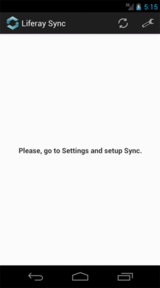
\includegraphics{../../images/liferay-sync-android-empty.png}
\caption{\\Figure 4.27: First screen}
\end{figure}

Touch the screen and it displays the \emph{Settings} view. You can
always go back to \emph{Settings} by clicking on the wrench icon at the
top right corner of the screen.

\begin{figure}[htbp]
\centering
\scalegraphics{../../images/liferay-sync-android-settings.png}
\caption{\\Figure 4.28: Android settings}
\end{figure}

Enter your Liferay server credentials by filling in your \emph{Login},
\emph{Password}, and \emph{Server} information. Your \emph{Login} is
either your user account's email address or screen name. Use the same
credentials you use to log in to the portal in a browser. In the
\emph{Server} field, enter your portal's URL. In this example, the
server URL is \emph{http://www.liferay.com}. Click the key icon on the
top right to test your connection and check if everything is correct.

Note for Gingerbread users: If you can't see some of the features
described here, click on the menu button to view a list of all possible
actions. This includes options to refresh, open the settings menu,
upload files, take photos, test your connection, etc.

\begin{figure}[htbp]
\centering
\scalegraphics{../../images/liferay-sync-android-gingerbread.png}
\caption{\\Figure 4.29: Gingerbread}
\end{figure}

After you have successfully tested your connection, hit the \emph{back}
button and you'll see a list of Liferay sites you have access to.

\begin{figure}[htbp]
\centering
\scalegraphics{../../images/liferay-sync-android-sites.png}
\caption{\\Figure 4.30: Sites}
\end{figure}

You can browse the files of a site by tapping on any of them. This opens
a list of the folders and files belonging to the site that you have
permission to view.

\begin{figure}[htbp]
\centering
\scalegraphics{../../images/liferay-sync-android-files-list.png}
\caption{\\Figure 4.31: Folder and files}
\end{figure}

From here, you can click on a folder and browse deeper into the folder
hierarchy or click the \emph{Back} button to navigate back to parent
folders up to the initial \emph{Sites} list.

Single-tap on a file to open it. If the file has never been downloaded
before, Sync will download it and open after it has finished
downloading. You can only view the file's contents if your device has an
app installed that can open the file type. For example, in order to open
a PDF, you must have at least one PDF viewer app installed. Otherwise,
you will see a message informing you that no viewer is available and you
need to install an app that can open the file.

Long-press on any folder or file to find a list of actions you can take
on it: \emph{Add to Favorites}, \emph{View Details}, \emph{Download},
\emph{Rename} or \emph{Delete}. This actions menu varies depending on
which entry type is selected: file or folder.

On Gingerbread, the actions menu looks like this:

\begin{figure}[htbp]
\centering
\scalegraphics{../../images/liferay-sync-android-gingerbread-context.png}
\caption{\\Figure 4.32: Gingerbread menu}
\end{figure}

On Ice Cream Sandwich and above, you can find the action icons and menu
at the top right:

\begin{figure}[htbp]
\centering
\scalegraphics{../../images/liferay-sync-android-ics-context.png}
\caption{\\Figure 4.33: ICS menu}
\end{figure}

Clicking on \emph{Add to Favorites} (Gingerbread) or the gray star (Ice
Cream Sandwich) adds the selected file to the \emph{Favorites} list.
\emph{Favorites} are special files that can be accessed and viewed even
when you are offline (more details below). If a file is already marked
as a favorite, you'll see a \emph{Remove from Favorites} or blue star
instead. Clicking on it removes the selected file from the
\emph{Favorites} list.

Clicking on \emph{View Details} (Gingerbread) or the round icon with the
letter ``i'' (Ice Cream Sandwich) opens the details view, which displays
the entry's metadata such as creation date, author, version,
description, etc.:

\begin{figure}[htbp]
\centering
\scalegraphics{../../images/liferay-sync-android-details.png}
\caption{\\Figure 4.34: View details}
\end{figure}

If you click on \emph{Download} (floppy disk icon on Ice Cream
Sandwich), it downloads and overwrites the local file copy.

You can rename a folder or file by clicking on the \emph{Rename} option.
This renames the entry in the portal.

Clicking on \emph{Delete} deletes the file/folder from the remote
portal, and other users won't be able to view or download it. On Ice
Cream Sandwich and above, you can select multiple entries for deletion:

\begin{figure}[htbp]
\centering
\scalegraphics{../../images/liferay-sync-android-delete.png}
\caption{\\Figure 4.35: Actions}
\end{figure}

Some actions are not related to a specific folder or file. You can find
these actions in the menu on the top action bar when no entry is
selected (Gingerbread users need to click on the device menu button).
Depending on the device screen width, some icons may overflow to the
three dots button on the right. Click on this button to see all of the
available actions.

\begin{figure}[htbp]
\centering
\scalegraphics{../../images/liferay-sync-android-more.png}
\caption{\\Figure 4.36: More options}
\end{figure}

The \emph{Refresh} button fetches and updates the list of folders and
files that have been changed in the portal.

The \emph{Camera} button allows you to quickly take a picture and upload
the image to the current folder. The image file name is automatically
generated with a time stamp.

The \emph{New Folder} button asks you for the name of the folder you
want to create in the portal.

The \emph{Upload} button displays the types of local files you can
upload to the portal. Choosing \emph{Image}, for example, shows all
images that are stored locally on your device. Once you choose the files
and confirm, these files are uploaded to the portal and are placed in
the current folder. By default, you can upload images, videos, and audio
files. If you have installed an app on your device that can open and
browse any type of file, you will also see an option called \emph{Other
files}.

\begin{figure}[htbp]
\centering
\scalegraphics{../../images/liferay-sync-android-upload.png}
\caption{\\Figure 4.37: Upload local files}
\end{figure}

The \emph{Favorites} menu option opens the favorites list. All files
that have been marked as favorites show up in this list. You should mark
your most important files as favorites because, as mentioned earlier,
the \emph{Favorites} feature gives you quick offline access to them. You
can view the contents of items in the \emph{Favorites} list, view their
metadata and, of course, remove them from the list.

\begin{figure}[htbp]
\centering
\scalegraphics{../../images/liferay-sync-android-favorites.png}
\caption{\\Figure 4.38: Favorites}
\end{figure}

Next, let's look at the iOS Sync app.

\subsubsection{iOS }

After installing Liferay Sync for iOS, an empty screen appears asking
you to set up the app. This screen appears whenever preferences are
missing.

\begin{figure}[htbp]
\centering
\scalegraphics{../../images/liferay-sync-ios-empty.png}
\caption{\\Figure 4.39: iOS Settings}
\end{figure}

Click on \emph{Settings} in the toolbar and enter your Liferay server
credentials by filling in your \emph{Login}, \emph{Password}, and
\emph{Server} information. Your \emph{Login} is either your user
account's email address or screen name, whichever you use to log in to
the portal in a browser. In the \emph{Server} field, enter your portal's
URL. In this example, the server URL is \emph{http://www.liferay.com}.
Click on \emph{Test Connection} to check if your configuration is
correct.

\begin{figure}[htbp]
\centering
\scalegraphics{../../images/liferay-sync-ios-settings.png}
\caption{\\Figure 4.40: iOS Settings}
\end{figure}

After you have successfully tested your connection, tap on the
\emph{Documents} toolbar section and you'll see a list of Liferay sites
you have access to.

\begin{figure}[htbp]
\centering
\scalegraphics{../../images/liferay-sync-ios-sites.png}
\caption{\\Figure 4.41: Sites}
\end{figure}

You can browse the files of a site by tapping on its name or icon. This
opens a list of the folders and files belonging to the site that you
have permission to view.

\begin{figure}[htbp]
\centering
\scalegraphics{../../images/liferay-sync-ios-files-list.png}
\caption{\\Figure 4.42: Folder and files}
\end{figure}

From here, you can click on a folder to browse deeper into the folder
hierarchy. You can also click on the \emph{Back} button to navigate back
to parent folders up to the initial \emph{Sites} list.

You can refresh the list by pushing it down. This updates all the files
and folders that have been changed in the portal.

\begin{figure}[htbp]
\centering
\scalegraphics{../../images/liferay-sync-ios-refresh.png}
\caption{\\Figure 4.43: Refreshing}
\end{figure}

When you click on a file, this file is downloaded from the remote portal
and, if a previewer for this file type is available, you can view the
contents of the file. The next time you open a file, it won't download
it again; instead, it opens the local copy.

\begin{figure}[htbp]
\centering
\scalegraphics{../../images/liferay-sync-ios-open.png}
\caption{\\Figure 4.44: Opening a file}
\end{figure}

There are 3 icons at the bottom of the screen when you open a file:

Clicking on the leftmost round icon with the letter ``i'' opens the
details view, which displays the entry's metadata such as creation date,
author, version, description, etc.:

\begin{figure}[htbp]
\centering
\scalegraphics{../../images/liferay-sync-ios-details.png}
\caption{\\Figure 4.45: View details}
\end{figure}

Clicking on the star icon at the center adds the selected file to the
\emph{Favorites} list. \emph{Favorites} are special files that can be
accessed and viewed even when you are offline (more details below). If a
file has already been marked as a favorite, clicking on the star icon
removes the file from the \emph{Favorites} list.

Clicking on the rightmost icon displays sharing options. You can, for
example, send the file as an email attachment, print the file, or copy
it to your clipboard. Some external apps may also appear in this list.
For example, you can share your file with social apps and messengers if
they are available.

\begin{figure}[htbp]
\centering
\scalegraphics{../../images/liferay-sync-ios-share.png}
\caption{\\Figure 4.46: Share options}
\end{figure}

In the file list, there's an Edit button. Clicking on it switches the
app to the edit mode as shown below:

\begin{figure}[htbp]
\centering
\scalegraphics{../../images/liferay-sync-ios-edit.png}
\caption{\\Figure 4.47: Edit mode}
\end{figure}

Selecting one or more files or folders and clicking on the \emph{Delete}
button deletes the selected files or folders from the remote portal.
Once you delete files or folders from the remote portal, other users
won't be able to view or download them.

Selecting only one file or folder enables the \emph{Rename} button.
Click on it to change the entry's name locally and remotely.

To quickly delete a file or folder from the portal, you can also swipe
right and click on the \emph{Delete} button in the file list view:

\begin{figure}[htbp]
\centering
\scalegraphics{../../images/liferay-sync-ios-delete.png}
\caption{\\Figure 4.48: Deleting a file}
\end{figure}

If you want to upload an image or video to the portal, click the
\emph{Plus} button at the top right corner. You should see three
options:

\emph{Take a photo or video} opens your camera app and lets you take a
photo or record a video and upload it.

\emph{Choose Existing} allows you to upload multiple photos or videos
stored on your device.

\emph{Create New Folder} lets you type the name of the folder and
creates it in the portal.

\begin{figure}[htbp]
\centering
\scalegraphics{../../images/liferay-sync-ios-more.png}
\caption{\\Figure 4.49: Upload photos and videos}
\end{figure}

The \emph{Favorites} toolbar section opens the favorites list. All files
that have been marked as favorites show up in this list. You should mark
your most important files as favorites because, as mentioned earlier,
the \emph{Favorites} feature gives you quick offline access to them. You
can view the contents of items in the \emph{Favorites} list, view their
metadata and, of course, remove them from the list.

\begin{figure}[htbp]
\centering
\scalegraphics{../../images/liferay-sync-ios-favorites.png}
\caption{\\Figure 4.50: Favorites}
\end{figure}

All downloaded files are stored on your device indefinitely.

\begin{figure}[htbp]
\centering
\scalegraphics{../../images/liferay-sync-ios-cache.png}
\caption{\\Figure 4.51: Deleting local copies}
\end{figure}

If you want to delete downloaded files locally but don't want to remove
them from the portal, go to \emph{Settings} and click on the \emph{Clear
Cache} button.

\section{Summary }

In this chapter, we examined Liferay's Documents and Media Library, a
powerful and customizable virtual shared drive. Liferay 6.1 introduced
the ability to mount multiple external repositories to the Documents and
Media library. The Documents and Media library can be used to store
files of any kind. The Documents and Media Display portlet is meant to
be configured to show chosen hierarchies of folders and files from the
Documents and Media library. The Media Gallery is meant for presenting
media files such as images or videos.

Document types and metadata sets provide a flexible way to distinguish
between different types of files and to define custom metadata fields
for them. Document previews are automatically generated by default, but
Liferay supports integration with external tools that offer greater
speed, higher quality, and additional functionality. Finally, we
discussed Liferay Sync, an add-on product for Liferay 6.1 that allows
your Liferay server to directly synchronize files on users' desktop and
mobile environments. 

\chapter{Leveraging the Asset Framework}


Any type of content in Liferay is considered an asset. In chapters 2 and
3, we already examined Liferay's most common type of asset: web content.
Other types of assets include blog posts, wiki articles, message board
posts, bookmarks, and documents. It's possible for developers to define
custom asset types that utilize Liferay's asset framework. Originally,
the asset framework was created to provide a mechanism for adding tags
to blog entries, wiki articles, and web content without reimplementing
the same functionality multiple times. The asset framework has been
greatly extended since then and it now supports tags, categories,
vocabularies, comments, ratings, and asset relationships.

This chapter covers the following topics:

\begin{itemize}
\item
  Tagging and categorizing content
\item
  Using targeted, single value, and multi-value vocabularies
\item
  Using Faceted Search
\item
  Using the Asset Publisher
\item
  Setting up display pages
\item
  Adding relationships between assets
\end{itemize}

The Asset Publisher portlet is designed to display multiple assets. It
has quite a few configuration options which we'll cover in this chapter.
By default, abstracts (previews) of recently published assets are
displayed by the Asset Publisher portlet and links to their full views
are provided. You can configure the Asset Publisher portlet to display a
table of assets, a list of asset titles, or the full content of assets.
You can also configure the Asset Publisher to display only certain kinds
of assets and you choose how many items to display in a list. The Asset
Publisher portlet is very useful for displaying chosen types of content,
for displaying recent content, and for allowing users to browse content
by tags and categories. The Asset Publisher is designed to integrate
with the Tags Navigation and Categories Navigation portlets to allow
this.

\section{Tagging and Categorizing Content
}

Tags and categories are two important tools you can use to help organize
information on your portal and make it easier for your users to find the
content they're looking for through search or navigation. Tagging and
categorizing web content is easy. You can do it at the bottom of the
same form you use to add content. If you open the \emph{Categorization}
section of the form, you'll be presented with an interface for adding
tags and categories.

\begin{figure}[htbp]
\centering
\scalegraphics{../../images/04-web-content-categorization.png}
\caption{Figure 5.1: Tagging and categorizing content can be done at the
same time you create it.}
\end{figure}

The Control Panel contains an interface for managing tags and categories
for each site in the portal. This interface can be used to manage all
your tags and categories in one place. It is important that you both tag
and categorize your content when you enter it. Let's take a closer look
at tags and categories.

\subsection{Tags }

Tags are an important tool that you can use to help organize information
on your portal and make it easier for your users to find content that
they're looking for. Tags are words or phrases that you can attach to
any content on the website. Tagging content will make your search
results more accurate, and enable you to use tools like the Asset
Publisher to display content in an organized fashion on a web page.
There are two ways to create tags: you can do it through the
administrative console in the Control Panel, or on the fly as content is
created.

\begin{figure}[htbp]
\centering
\scalegraphics{../../images/05-add-tag.png}
\caption{Figure 5.2: The Add Tag Dialog}
\end{figure}

To create tags in the Control Panel, select the site that you want to
create tags for, and select \emph{Tags}. From this screen, you will be
able to view any existing tags and make new ones. To create a new tag,
simply click \emph{Add Tag}. You'll then be asked for the name of the
tag, and you'll have the ability to set permissions for viewing or
managing the tag. You can also add properties to a tag. Properties
basically act like tags for your tags. Structurally, properties are
key-value pairs associated with specific tags that provide information
about your tags. You can edit existing tags from the \emph{Tags} window
of on the Control Panel. You can change the tag name, change the tag's
permissions, delete the tag, or add properties.

Tags are not the only portal-wide mechanism for describing content: you
can also use categories.

\subsection{Categories }

Categories are similar in concept to tags, but are designed for use by
administrators, not regular users. Hierarchies of categories can be
created, and categories can be grouped together in \emph{vocabularies}.
While tags represent an ad hoc method for users to group content
together, categories exist to allow administrators to organize content
in a more official, hierarchical structure. You can think of tags like
the index of a book and categories like its table of contents. Both
serve the same purpose: to help users find the information they seek.

Adding vocabularies and categories is similar to adding tags. Once
you've selected the site you want to work on, select \emph{Categories}
from the content section of the Control Panel, and you will be presented
with the categories administration page.

\begin{figure}[htbp]
\centering
\scalegraphics{../../images/05-categories.png}
\caption{Figure 5.3: Categories Administration Page}
\end{figure}

Clicking on a vocabulary on the left displays any categories that have
been created under that vocabulary. You can create new vocabularies
simply by clicking \emph{Add Vocabulary} and providing a name for it.
You can create categories in a similar fashion by choosing a vocabulary
on the left, and then selecting \emph{Add Category}. Like tags, you can
also provide properties for categories. Once you have created some
vocabularies and categories, you can take advantage of the full
capabilities of categories by creating a nested hierarchy of categories.
To nest categories, select what you want to be the parent category, then
drag any category that you want to become a child category onto it. You
will see a plus sign appear next to the name of the category you are
dragging if you can add it to the selected parent category; if you see a
red \emph{x} that means that you cannot add that category as a
subcategory of parent category that you have selected.

Once you have created a hierarchy of categories, your content creators
will have them available to apply to content that they create. Navigate
to the Web Content page of the Control Panel and click \emph{Add
Content}. Click the Categorization link from the right-side menu and
click \emph{Select} on the vocabulary you would like to use. A dialog
box will appear with your categories. Select any relevant categories by
checking the box next to them, and they will be applied to the content.

There are a several new enhancements to vocabularies and categories in
Liferay 6.1. The three main features are targeted vocabularies,
single/multi-valued vocabularies, and separated widgets for every
vocabulary.

\section{Targeted Vocabularies
}

Targeted Vocabularies allow you to decide which vocabularies can be
applied to an asset type and which vocabularies are required for an
asset type. To configure these settings, go to the categories
administration page and mouse over the vocabulary in the list until you
see the edit icon to the right. Select the icon to reveal a dialog box
like the one below.

\begin{figure}[htbp]
\centering
\scalegraphics{../../images/targeted-vocabularies.png}
\caption{Figure 5.4: You can target vocabularies by checking the
\emph{Allow Multiple Categories} checkbox and then selecting the Asset
Types.}
\end{figure}

The default value for \emph{Associated Asset Types} is \emph{All Asset
Types}. You can fine tune your choices by using the \emph{+} and
\emph{-} buttons, which narrows the scope of the vocabulary to specific
assets. In the screenshot above, notice how the vocabulary
\texttt{Famous Noses} is configured to be available for Blogs and Web
Content, but it is not required. It is mandatory, however, for Documents
and Media Documents.

\subsection{Single and Multi-valued Vocabularies
}

You can now decide if the user can choose one or more categories from
the same vocabulary to categorize an asset. If a vocabulary is
single-valued you can only choose one, and if it allows more, you can
choose several categories.

\begin{figure}[htbp]
\centering
\scalegraphics{../../images/multi-valued-vocabularies.png}
\caption{Figure 5.5: Single-valued vocabularies, on the left, use radio
buttons while multi-valued vocabularies use checkboxes. .}
\end{figure}

Setting vocabulary values is done through the categories administration
page. Edit a vocabulary and deselect the \emph{Allow Multiple
Categories} checkbox to set single value vocabularies or use the default
option to set multi-value vocabularies.

\subsection{Separated Widgets
}

The third important improvement is every vocabulary has its own
separated widget. These widgets appear in the Categorization section of
every asset and they allow users to easily select appropriate categories
for that asset.

\begin{figure}[htbp]
\centering
\scalegraphics{../../images/separated-widgets.png}
\caption{Figure 5.6: Now that vocabularies have their own widgets, it's
easy to select available categories.}
\end{figure}

It's important to use tags and categories with all your content, so that
content is easier for users to find. Let's look at one of the ways users
will make use of tags and categories: searching for content.

\section{Using Faceted Search
}

To stay organized, I (RS) used to use a paper-based planner. It had
various sections for various areas of my life. Its initial incarnation
came from a commercial company, but over the years I tweaked it into
something that worked for me. This final version (before I went digital)
had different tabs for different areas of my life that I wanted to keep
track of: daily items like tasks, notes, a spiritual section, and agenda
pages that kept track of things I needed to go over with specific
people. A Planning section had tabs for projects, family, future items,
and reference.

Of course, since this was paper-based, it had its limitations. It was
kind of hard to find stuff. Did I put the note I'd written about that
new toy my daughter wanted in the Notes section or in the Family
section? Or maybe it was on my \emph{While Out} list, so I would
remember to buy it before her birthday?

Liferay content can be like this. That important information you
remember seeing--was it in a wiki article, a message boards post, or web
content? Did you remember to tag it? If you don't have this kind of
information, browsing to the content you're looking for could be
difficult. Thankfully, Liferay includes a powerful, faceted search
function, which means you can drill down through the different types of
content, tags, and categories to refine your search and find what you
want. Let's see how to use it.

\subsection{Searching for Portal Content
}

To get started, drop the Search portlet on a page and search for
something. You'll see a page with results on the right and a collection
of \emph{facets} on the left.

\begin{figure}[htbp]
\centering
\scalegraphics{../../images/faceted-search-1.png}
\caption{\\Figure 5.7: The first set of facets is content types. You can
drill down to specific types of content that contain the search terms
you entered.}
\end{figure}

A facet is a combination of the information about a specific indexed
field, its terms, and their frequency. Facets are typically named by the
field in question. The default facets are asset types (pictured above),
asset tags, asset categories, and modified time range.

The frequency in which the term was found for each facet is listed in
parentheses after the facet. It may jog your memory to see that the term
you searched for appears in a blog entry, and that may be all you need
to find what you were looking for. If, however, your memory is more
foggy than that, or you're searching for something you're not sure is
actually there, then the asset tags or asset categories facets may be
more helpful to you.

\begin{figure}[htbp]
\centering
\scalegraphics{../../images/faceted-search-2.png}
\caption{Figure 5.8: Asset tag facets provide you with more information
list, and the results to the right are refined by the facet you
selected.}
\end{figure}

\begin{figure}[htbp]
\centering
\scalegraphics{../../images/05-faceted-search-drill-down-1.png}
\caption{\\Figure 5.9: Drilling down creates a list of what you selected
at the top of the screen.}
\end{figure}

Here we can see that we've selected one of the tags, \emph{liferay}, to
further refine the search. The tag appears in a list at the top, and
there's a red X next to it that lets us remove it from our filter as we
work to increase the relevancy of our search. But maybe selecting only
the tag isn't enough to filter our search into something small enough to
sort through. In this case, we can further refine the search by
selecting another facet, as below.

\begin{figure}[htbp]
\centering
\scalegraphics{../../images/05-faceted-search-drill-down-2.png}
\caption{\\Figure 5.10: Selecting another facet further refines the
search.}
\end{figure}

Now we've selected web content, which is one particular content type
within Liferay, and the list of potential hits on our search terms has
been dramatically reduced. In this way, you can interactively tweak the
search results to narrow them down, making it easier to find that
proverbial needle within the haystack.

\subsubsection{Asset Types }

Searching can only be done on assets. As has already been described in
this chapter, just about any entity in the portal is an asset and can be
indexed and searched. Under the hood, this means that these entities use
Liferay's Asset API and have an Indexer defined.

Developers can create custom searchable assets within the portal. This
is described in the
\href{https://www.liferay.com/documentation/liferay-portal/6.1/development/-/ai/-asset-framewo-1}{Developer's
Guide}. For this reason, you may have additional asset types defined in
your portal beyond the ones that Liferay ships with by default. If this
is the case, you may wish to tweak the \texttt{frequency threshold} and
the \texttt{max terms} settings to increase the number of asset types
displayed past the default of 10. This is covered in the section below
on search options.

\subsubsection{Asset Tags }

If tags have been applied to any asset that appears in the result set,
it may be displayed in the Asset Tag facet. Tags are handled in a
similar way to how asset types are handled: not all tags may appear.
There may be many more than the 10 tags listed, but the default
configuration for this facet is to show the top 10 most frequent terms.
As with asset types, this can be modified by setting \texttt{max terms}
property.

\subsubsection{Asset Categories
}

If categories have been applied to any asset that appears in the result
set, they may be displayed in the Asset Categories facet. Yadda, yadda,
yadda, same thing as the two sections above. That last sentence was
written to check if you're still reading.

Let's move on to advanced searching.

\subsection{Advanced Searching
}

The Search portlet's search box is deceptively simple. Though you have
only a single field for search, there's a search syntax inherited from
\href{http://lucene.apache.org/core/old\_versioned\_docs/versions/3\_0\_3/queryparsersyntax.html}{Lucene}
that lets you create very powerful search queries. Let's look at some
ways you can use search queries.

\textbf{Searching for specific fields:} By default, searches are
performed against a long list of fields. Sometimes you want results for
a term within a particular field. This can be achieved using the field
search syntax \texttt{{[}field{]}:{[}term{]}}. For example, to search in
the \emph{Title} field for \emph{Liferay}, use the following syntax:

\begin{verbatim}
title:liferay
\end{verbatim}

If you search for a phrase within a field, surround the term with double
quotation marks:

\begin{verbatim}
title:"Liferay Portal"
\end{verbatim}

\textbf{Wildcards:} You can use wildcards in exactly the way you use
them with your operating system: for a single character wildcard, use
\texttt{?}; for the multiple character wildcard, use \texttt{*}.

\textbf{Boolean operators:} You can use logic operators, such as AND,
OR, NOT, \texttt{+}, and \texttt{-} in your searches. The \texttt{AND}
operator matches assets in which the terms between the \texttt{AND}
operator exist. For example, to search for both Liferay and Kaleo
Workflow, use this query:

\begin{verbatim}
"liferay" AND "kaleo workflow"
\end{verbatim}

The \texttt{OR} operator is the default; if there's no operator between
two terms, the \texttt{OR} operator takes effect. \texttt{OR} finds
matches if any term exists in an asset.

The \texttt{+} operator requires that the term exists somewhere in some
field in the asset. If you wanted to search for something that
\emph{must} contain \emph{liferay} and \emph{may} contain \emph{portal},
use this query:

\begin{verbatim}
+liferay portal
\end{verbatim}

The \texttt{NOT} operator excludes assets that contain the term after
the \texttt{NOT} operator. It requires that at least two terms be
present:

\begin{verbatim}
"Liferay Portal" NOT "Liferay Social Office" 
\end{verbatim}

The \texttt{-} operator is similar: it excludes assets that contain the
term after the \texttt{-} symbol:

\begin{verbatim}
"Liferay Portal" - "Liferay Social Office" 
\end{verbatim}

\textbf{Grouping:} You can use parentheses within your queries to form
sub-queries, in a similar fashion to an SQL statement. For example, to
search for \emph{liferay} or \emph{social office} and \emph{website},
use this query:

\begin{verbatim}
(liferay OR "social office") AND website
\end{verbatim}

As you can see, the search syntax is very powerful. There's more you can
do with it than what is listed here; to view the full syntax, visit the
Lucene URL above.

Next, we'll look at how the Search portlet can be configured.

\subsection{Setting Search Options
}

As with Liferay's other portlets, you can configure the Search portlet
via the configuration screen, which looks like the below illustration.

\begin{figure}[htbp]
\centering
\scalegraphics{../../images/05-faceted-search-configuration.png}
\caption{Figure 5.11: Basic search configuration is pretty
straightforward.}
\end{figure}

\textbf{Display Asset Type Facet:} Toggles whether the Asset Type facet
appears.

\textbf{Display Asset Tags Facet:} Toggles whether the Asset Tags facet
appears.

\textbf{Display Asset Categories Facet:} Toggles whether the Asset
Categories facet appears.

\textbf{Display Modified Range Facet:} Toggles whether the date modified
range facet appears.

\textbf{Display Results in Document Form:} Never use this in production.
Developers use this feature to view search responses in their generic,
Document-based format. Part of a developer's job when writing search
indexers is to convert Documents (the objects that get indexed) to the
actual object and back again. This option allows developers to see how
their objects are being indexed.

\textbf{View in Context:} When an asset is clicked, show it in the
portlet to which it belongs.

\textbf{Display Main Query:} Show the exact search query that the
portlet generated to the search engine. Again, never use this in
production; this is for development purposes only.

\textbf{Display Open Search Results:} Shows results from third party
Open Search plugins, if they are installed. This is for backward
compatibility only: developers are encouraged to re-design their search
code as described in \emph{Liferay in Action}, and then custom assets
are aggregated with native portal assets seamlessly.

These are the basic options, but surely you didn't miss the fact that
there are also advanced options.

Configuring advanced search requires a bit more technical acumen than
you might expect, because there are so many properties to tweak.
Thankfully, in most instances, you shouldn't need to change a thing. If
you do, however, the configuration is done through a JSON object.

If you don't know what a JSON object is, don't worry: it's not a
difficult concept. JSON stands for \textbf{J}ava\textbf{S}cript
\textbf{O}bject \textbf{N}otation. An Object is a software development
term for anything that can be represented in code. Objects have
\emph{attributes}, or sometimes these are called \emph{fields}, and they
are very similar to fields you'd find on a form that you're filling out.
Software developers use the word \emph{object} to refer generically to
anything like this that they can describe in the software; for all
intents and purposes, objects could just as easily have been called
Things. For example, one type of object used in Liferay is a User. A
User can be represented in code, and it has many \emph{fields}, such as
a name, an email address, and more. JSON is one way of describing
objects like this.

The object we're concerned with is called \texttt{facets}. Here's what
it looks like, in all its glory, in JSON. Explanation of the settings
follows the object below.

\begin{verbatim}
{"facets": [
    {
    "displayStyle": "asset_entries",
    "weight": 1.5,
    "static": false,
    "order": "OrderHitsDesc",
    "data": {
        "values": [
        "com.liferay.portlet.bookmarks.model.BookmarksEntry",
        "com.liferay.portlet.blogs.model.BlogsEntry",
        "com.liferay.portlet.calendar.model.CalEvent",
        "com.liferay.portlet.documentlibrary.model.DLFileEntry",
        "com.liferay.portlet.journal.model.JournalArticle",
        "com.liferay.portlet.messageboards.model.MBMessage",
        "com.liferay.portlet.wiki.model.WikiPage",
        "com.liferay.portal.model.User"
        ],
        "frequencyThreshold": 1
    },
    "label": "asset-type",
    "className": "com.liferay.portal.kernel.search.facet.AssetEntriesFacet",
    "fieldName": "entryClassName"
    },
    {
    "displayStyle": "asset_tags",
    "weight": 1.4,
    "static": false,
    "order": "OrderHitsDesc",
    "data": {
        "maxTerms": 10,
        "displayStyle": "list",
        "frequencyThreshold": 1,
        "showAssetCount": true
    },
    "label": "tag",
    "className": "com.liferay.portal.kernel.search.facet.MultiValueFacet",
    "fieldName": "assetTagNames"
    },
    {
    "displayStyle": "asset_tags",
    "weight": 1.3,
    "static": false,
    "order": "OrderHitsDesc",
    "data": {
        "maxTerms": 10,
        "displayStyle": "list",
        "frequencyThreshold": 1,
        "showAssetCount": true
    },
    "label": "category",
    "className": "com.liferay.portal.kernel.search.facet.MultiValueFacet",
    "fieldName": "assetCategoryTitles"
    },
    {
    "displayStyle": "modified",
    "weight": 1.1,
    "static": false,
    "order": "OrderHitsDesc",
    "data": {
        "ranges": [
        {
            "range": "[past-hour TO *]",
            "label": "past-hour"
        },
        {
            "range": "[past-24-hours TO *]",
            "label": "past-24-hours"
        },
        {
            "range": "[past-week TO *]",
            "label": "past-week"
        },
        {
            "range": "[past-month TO *]",
            "label": "past-month"
        },
        {
            "range": "[past-year TO *]",
            "label": "past-year"
        }
        ],
        "frequencyThreshold": 0
    },
    "label": "modified",
    "className": "com.liferay.portal.kernel.search.facet.ModifiedFacet",
    "fieldName": "modified"
    }
]}
\end{verbatim}

Now that you've seen the object, don't be daunted by it. Here are all
the settings within the object that you can tweak.

\textbf{``className'':} This field must contain a string value which is
the FQCN (fully qualified class name) of a java implementation class
implementing the Facet interface. Liferay provides the following
implementations by default:

\begin{verbatim}
com.liferay.portal.kernel.search.facet.AssetEntriesFacet
com.liferay.portal.kernel.search.facet.ModifiedFacet
com.liferay.portal.kernel.search.facet.MultiValueFacet
com.liferay.portal.kernel.search.facet.RangeFacet
com.liferay.portal.kernel.search.facet.ScopeFacet
com.liferay.portal.kernel.search.facet.SimpleFacet
\end{verbatim}

\textbf{``data'':} This field takes an arbitrary JSON object (a.k.a.
\{\}) for use by a specific facet implementation. As such, there is no
fixed definition of the data field. Each implementation is free to
structure it as needed. The value defined here matches the
implementation that's selected in the \texttt{className} attribute
above.

\textbf{``displayStyle'':} This field takes a string value and
represents a particular template implementation which is used to render
the facet. These templates are normally JSP pages (but can also be
implemented as Velocity or Freemarker templates provided by a theme if
the portal property \texttt{theme.jsp.over\-ride.en\-abled} is set to
\texttt{true}). The method of matching the string to a JSP is simply
done by prefixing the string with /html/portlet/search/facets/ and
appending the .jsp extension.

For example, \texttt{"displayStyle": "asset\_tags"} maps to the JSP

\begin{verbatim}
/html/portlet/search/facets/asset_tags.jsp
\end{verbatim}

Armed with this knowledge a crafty developer could create custom display
styles by deploying custom (new or overriding) JSPs using a JSP hook.
See the \emph{Developer's Guide} or \emph{Liferay in Action} for more
information on hook plugins.

\textbf{``fieldName'':} This field takes a string value and defines the
indexed field on which the facet operates.

For example, \texttt{"fieldName": "entryClassName"} indicates that the
specified facet implementation operates on the \texttt{entryClassName}
indexed field.

\textbf{Note:} You can identify available indexed fields by enabling the
Search portlet's \emph{Display Results in Document Form} configuration
setting and then expanding individual results by clicking the {[}+{]} to
the left of their titles.

\textbf{``label'':} This field takes a string value and represents the
language key that is used for localizing the title of the facet when
it's rendered.

\textbf{``order'':} This field takes a string value. There are two
possible values:

\texttt{OrderValueAsc}: This tells the facet to sort it's results by the
term values, in ascending order.

\texttt{OrderHitsDesc}: This tells the facet to sort it's results by the
term frequency, in descending order.

\textbf{``static'':} This field takes a boolean value (\texttt{true} or
\texttt{false}). The default value is false. A value of \texttt{true}
means that the facet should not actually be rendered in the UI. It also
means that it should use pre-set values (stored in its \texttt{data}
field) rather than inputs dynamically applied by the end user. This
allows for the creation of pre-configured search results.

Imagine you would like to create a pre-configured search that returns
only images (i.e.~the asset type is
\texttt{DLFileEntry} and the
indexed field extension should contain the values bmp, gif, jpeg, jpg,
odg, png, or svg). We would need two static facets, one with
``fieldName'': ``entryClassName'' and another with ``fieldName'':
``extension''. This could be represented using the following facet
configuration:

\begin{verbatim}
{
    "displayStyle": "asset_entries",
    "static": true,
    "weight": 1.5,
    "order": "OrderHitsDesc",
    "data": {
    "values": [
        "com.liferay.portlet.documentlibrary.model.DLFileEntry"
    ],
    "frequencyThreshold": 0
    },
    "className": "com.liferay.portal.kernel.search.facet.AssetEntriesFacet",
    "label": "asset-type",
    "fieldName": "entryClassName"
},
{
    "displayStyle": "asset_entries",
    "static": true,
    "weight": 1.5,
    "order": "OrderHitsDesc",
    "data": {
    "values": ["bmp", "gif", "jpeg", "jpg", "odg", "png", "svg"],
    "frequencyThreshold": 0
    },
    "className": "com.liferay.portal.kernel.search.facet.MultiValueFacet",
    "label": "images",
    "fieldName": "extension"
}
\end{verbatim}

\textbf{``weight'':} This field takes a floating point (or double) value
and is used to determine the ordering of the facets in the facet column
of the search portlet. Facets are positioned with the largest values at
the top. (yes, the current implementation is counter-intuitive and
perhaps could be reversed in future versions).

Configuring search using a JSON object is a bit unusual, but as you can
see, it's not as hard as it looks initially.

\subsection{Summary }

Search is a powerful component of Liferay Portal's asset framework. The
proclivity of assets means that there is an extensible, robust, and
configurable search mechanism throughout the portal that allows
administrators to optimize the search experience of their users. Users
also get an easy to use search interface that makes use of the tags and
categories that they themselves apply to various pieces of content,
regardless of the type of content. This makes Liferay's search truly
``for the people.''

Power users can learn an extended search syntax that lets them craft
very specific searches. These searches can be used on large
installations with lots of data to find the proverbial needle in the
proverbial haystack. Administrators can tune the configuration of search
portlets so that they are optimized for the contents of their
communities.

Next, we'll look at how the Asset Publisher portlet makes even more
extensive use of Liferay's asset framework to bring relevant content to
users.

\section{Using the Asset Publisher
}

As we create web content, it's important to keep in mind that to
Liferay, the pieces of content are assets, just like message board
entries and blog posts. This allows you to publish your web content
using Liferay's Asset Publisher.

You can use the Asset Publisher to publish a mixed group of various
kinds of assets such as images, documents, blogs, and of course, web
content. This helps in creating a more dynamic web site: you can place
user-created wiki entries, blog posts or message board messages in
context with your content. Let's look at some of its features.

\subsubsection{Querying for Content
}

The Asset Publisher portlet is a highly configurable application that
lets you query for mixed types of content on the fly. By giving you the
ability to control what and how content is displayed from one location,
the Asset Publisher helps you to ``bubble up'' the most relevant content
to your users.

To get to all the portlet's options, click the \emph{Configuration} link
in the portlet's menu (the wrench icon).

The ability to configure how content is displayed and selected by your
users further demonstrates the flexibility of the Asset Publisher. You
get to choose how content is displayed. You can select it manually for
display in a similar way to the Web Content Display portlet or you can
set up predefined queries and filters and let the portal select the
content for you, based on its type or its tags and categories.

Let's first look at how we might select content manually. You'll see
that it's very similar to the Web Content Display portlet.

\paragraph{Selecting assets manually
}

By selecting \emph{Manual} from the select box beneath \emph{Asset
Selection}, you tell the Asset Publisher that you want to select content
manually. You can select what you want to be published within the
portlet, or you can create new content from within the Asset Publisher.

\begin{figure}[htbp]
\centering
\scalegraphics{../../images/04-web-content-asset-publisher-manual.png}
\caption{Figure 5.12: Selecting assets manually is very similar to the
Web Content Display portlet, except you have many other content types to
choose from.}
\end{figure}

Clicking \emph{Add New} gives you a menu of options, enabling you to
create the content right where you are. You can create blogs, bookmarks,
calendar entries, documents, images, and of course, web content.
Anything you create here is added to the list below of assets that are
displayed by the portlet.

Clicking \emph{Select Existing} gives you a similar menu, except this
time you can pick from existing content in the portal that either you or
your users have created. Has someone written an excellent wiki page that
you want to highlight? Select it here, and it will be displayed.

The Asset Publisher enables you to mix and match different content types
in the same interface. Once you have your content selected, you can move
on to the display types to configure how the content appears.

Most of the time, however, you'll likely be using the Asset Publisher to
select content dynamically.

\paragraph{Selecting assets dynamically
}

The Asset Publisher's default behavior is to select assets dynamically
according to rules that you give it. These rules can be stacked on top
of each other so that they compliment each other to create a nice,
refined query for your content. You have the following options for
creating these rules:

\textbf{Scope:} Choose the sites or organizations from which the content
should be selected.

\textbf{Asset Type:} Choose whether you'll display any asset or only
assets of a specific type, such as only web content, only wiki entries,
or any combinations of multiple types.

\begin{figure}[htbp]
\centering
\scalegraphics{../../images/04-web-content-asset-publisher-filter.png}
\caption{Figure 5.13: You can filter by tags and categories, and you can
set up as many filter rules as you need.}
\end{figure}

\textbf{Filter Rules:} Add as many filters on tags or categories as you
like. You can choose whether the content contains or does not contain
any or all categories or tags that you enter.

Once you've set up your filter rules for dynamically selecting your
content, you can then decide how the content will be displayed.

The Display Settings section gives you precise control over the display
of your assets. There are a multitude of options available to configure
how you want your content to appear. You can configure the style, length
of abstracts, behavior of the asset link, maximum items to display,
pagination type and file conversions. Additionally, you can enable
printing, flags, ratings, comments and comment ratings, and these work
the same way they do in the Web Content Display portlet.

You can display the content returned by the filters above in order by
title, create date, modified date, view count and more in ascending or
descending order. For instance, you may have a series of ``How To''
articles that you want displayed in descending order based on whether
the article was tagged with the \emph{hammer} tag. Or, you may want a
series of video captures to display in ascending order based on a
category called \emph{birds}. You can also group by \emph{Asset},
\emph{Type} or \emph{Vocabularies}. Vocabularies are groups of
categories defined by administrators in the \emph{Categories} section of
the Control Panel.

In the \emph{Ordering and Grouping} section of the Asset Publisher, you
have great control over how content is ordered and grouped in the list,
but this is only one aspect of how your content will be displayed. You
can refine the display through many other display settings.

\section{Setting up Display Pages
}

The Display Settings section gives you precise control over the display
of your assets. There are a multitude of options available to configure
how you want your content to appear. You can configure the style, length
of abstracts, behavior of the asset link, maximum items to display,
pagination type and file conversions. Additionally, you can enable
printing, flags, ratings, comments and comment ratings, and these work
the same way they do in the Web Content Display portlet.

\paragraph{Display Style }

\textbf{Abstracts:} Shows the first 200-500 characters of the content,
defined by the \textbf{Abstract Length} field.

\textbf{Table:} Displays the content in an HTML table which can be
styled by a theme developer.

\textbf{Title List:} The content's title as defined by the user who
entered it.

\textbf{Full Content:} The entire content of the entry.

\paragraph{Other Settings }

\textbf{Asset Link Behavior:} The default value is \emph{Show Full
Content}. With this value selected, when the link to an asset is
clicked, the full asset is displayed in the current Asset Publisher. If
the value \emph{View in a Specific Portlet} is selected, clicking on an
asset causes that asset to be displayed in the portlet to which the
asset belongs. For example, a blog entry would be displayed in the Blogs
portlet where it was created. Likewise, a forum post would be displayed
in the Message Boards porlet where it was created. Similarly, a generic
Web Content article would be displayed in the Asset Publisher of its
configurated Display Page. See the secton below on Display Pages for
more information.

\textbf{Maximum Items to Display:} You can display 1-100 items.

\textbf{Pagination Type:} Select Simple or Regular. Simple shows
previous and next navigation; regular includes a way of selecting the
page to which you'd like to navigate.

\textbf{Exclude Assets with 0 Views:} If an asset has not been viewed,
exclude it from the list.

\textbf{Show Available Locales:} Since content can be localized, you can
have different versions of it based on locale. This will show the
locales available, enabling the user to view the content in the language
of his or her choice.

\textbf{Enable Conversion To:} If you have enabled Liferay Portal's
OpenOffice.org integration, you can allow your users to convert the
content to one of several formats, including PDF.

Below these options are the same ones in the Web Content Display
portlet: enable print, enable comments, enable ratings, etc.

\textbf{Show Metadata:} Allows you to select from the available metadata
types (see below).

\begin{figure}[htbp]
\centering
\scalegraphics{../../images/available-metadata-fields.png}
\caption{Figure 5.14: Available metadata types}
\end{figure}

\textbf{Enable RSS Subscription:} This lets users subscribe to the
content via RSS Feeds.

The Display Settings section of the Asset Publisher has numerous options
to help you configure how your content selections are displayed to your
users. Even though there are many choices, it's easy to go through the
options and quickly adjust the ones that apply to you. You'll want to
use the Asset Publisher to query for mixed assets in the portal that
have relevant information for your users.

Next, we'll look at Display Pages, an addition to the asset framework
introduced by Liferay 6.1.

\subsubsection{Display Page }

If you've been using Liferay for a while, or you've just spent a little
bit of time with this guide, you might have noticed something about how
Liferay handles web content--content is never tied directly to a page.
While this can be useful (because it means that you don't have to
recreate content if you want to display the same thing on multiple
pages), it also means that you don't have a static URL for any web
content, which is bad for search engine optimization.

As an improvement, Liferay has introduced the concept of Display Pages
and Canonical URLs. Each web content entry on the portal has a canonical
URL, which is the official location of the content that is referenced
any time the content is displayed. A Display Page can be any page with
an asset publisher configured to display any content associated with the
page. When adding or editing web content articles, you can select a
Display Page, but only pages with a configured asset publisher are
available for selection.

To create a Display Page, you can create a page yourself, add an Asset
Publisher portlet and configure it yourself. Alternatively, you can use
the \emph{Content Display Page} page template included with Liferay. If
you're creating a Display Page manually, once you've added an Asset
Publisher portlet to the page, open its configuration window. Then check
the \emph{Set as the Default Asset Publisher for This Page} box.

You may now be thinking, ``Wait, you just told me that each Web Content
item has its own URL, and that this is somehow related to pages where we
display a whole bunch of content on the same page?'' Yes. That's exactly
what I said. Just watch--create a display page called \emph{My Web
Content Display Page} somewhere on your portal, using the \emph{Content
Display Page} template. Now, on a different page, add a Web Content
Display portlet. Click the \emph{Add Web Content} button, enter a title
and some content, click on \emph{Display Page} at the right, and select
the Display Page you just created. Then click \emph{Publish}.

\begin{figure}[htbp]
\centering
\scalegraphics{../../images/04-web-content-display-page.png}
\caption{Figure 5.15: Selecting a Display Page}
\end{figure}

In the Asset Publisher of the \emph{My Web Content Display Page}, you
can now click the \emph{Read More} link to display the content. Notice
that the canonical URL for content appears in your browser's address
bar. If you create your own custom display page, any additional portlets
that you place on the page are displayed along with the content when you
access it via the canonical URL. If you used the \emph{Content Display
Page} page template for your Display page, it not only features a
configured Asset Publisher portlet but also a Tags Navigation, a
Categories Navigation, and a Search portlet. These tools help users to
quickly identify relevant content.

\begin{figure}[htbp]
\centering
\scalegraphics{../../images/04-web-content-canonical-url.png}
\caption{Figure 5.16: The Canonical URL}
\end{figure}

Let's move on to another new featured introduced by Liferay 6.1.

\section{Defining content relationships }

Related Assets is a new feature in Liferay 6.1 that enables you to
connect any number of assets within a site or across the portal, even if
they don't share any tags and aren't in the same category. We've already
seen that you can show related assets within the display for a specific
asset, and with the Related Assets portlet you can show links to any
assets which are related to content displayed on that page.

The Related Assets portlet is based on the Asset Publisher and possseses
essentially the same interface with one key difference. The Asset
publisher displays any content that meets the criteria selected in the
portlet configuration. The Related Assets portlet only displays content
that meets the criteria, and also is listed as a related asset for a
piece of content that is currently published on the page where it is
placed. Let's take a look at the the Related Assets portlet.

As a prerequisite for the Related Assets portlet to display related
assets, you configure it to show the content you want displayed. To do
this, go to the Asset Publisher portlet and select the \emph{wrench}
icon in the upper right corner of the portlet. Under the \emph{Setup}
tab, set type of asset(s) to display using the \emph{Asset Type} menu.
The default value is set to \emph{Any}. You can narrow the scope of the
portlet to display any single category of asset type or select multiple
assets from the menu.

Filter options let you set minimum requirements for displaying assets by
their categories, tags, and custom fields. Ordering and Grouping allows
you to organize assets using the same criteria. Display settings allow
you to customize how asssets are shown in the portlet. They can be
listed by title, in a table, by abstract or full content. You can
convert assets to different document types like ODT, PDF, and RTF. You
can choose to show various metadata fields such as author, modification
date, tags, and view count. You can even enable RSS subscriptions and
customize their display settings.

When you are finished setting the Source and Filter options, click
\emph{Save}. But hold on a minute. You saw the message that says,
\texttt{You have successfully updated the setup}, but there still aren't
any assets displayed in the related assets portlet. Why? You cannot see
any related assets until you select an asset in the Asset Publisher.

\begin{figure}[htbp]
\centering
\scalegraphics{../../images/related-assets-portlet-after.png}
\caption{Figure 5.17: Select an asset in the Asset Publisher to see its
related assets displayed in the Related Assets portlet.}
\end{figure}

Once you select an asset, its related assets will display in the Related
Assets portlet, similar to the image above.

\section{Summary }

In this chapter, we explored Liferay's asset framework. Any type of
content in Liferay is considered an asset and can utilize the features
provided by the asset framework: tags, categories, comments, ratings,
and relationships. We examined the Asset Publisher portlet and looked at
the many configuration options for choosing what kinds of assets to
display and how to display them. We saw that the Asset Publisher portlet
is designed to integrate with the Tags Navigation and Categories
navigation portlets to allow users to browse content more easily. We
also learned about the Display Page attribute of web content, the
Content Display Page page template, and canonical URLs for assets.
Assets can have display page associated with them so that the full view
of the asset is displayed on the display page. The display page of an
asset is used in the asset's canonical URL. 

\chapter{Personalization and Customization}

In this chapter, we discuss several ways Liferay users can customize
pages, applications, and the way they use your portal. We'll cover the
following topics:

\begin{itemize}
\item
  Personal Sites
\item
  Customizable Pages and Applications
\item
  Using a Rules Engine
\end{itemize}

Personal sites allow each portal user to manage and customize a set of
public and/or private pages and any associated content or applications.
Public pages provide a means of making content publicly available while
private pages provide a means of hiding information from other users.
Liferay 6.1 introduced customizable pages and applications.
Administrators can designate certain pages or applications as
``customizable,'' which allows each user to make and save their own
customizations. Liferay Enterprise Edition provides a rules engine which
allows administrators to create custom portal rules and simplify complex
blocks of code containing lots of \texttt{if-else} statements. Let's
start by discussing personal sites.

\section{User Personal Sites
}

By default, newly created users in Liferay are each granted a personal
site. Each user functions as the site administrator of his or her
personal site. Personal sites are fully customizable but cannot have
more than one member. The public pages of personal sites provide a space
for users to publish content that they'd like to make accessible to
anyone, including guests. User blogs are often placed on public personal
site pages. Content and applications that users would like to reserve
for personal use are often placed on the private pages of personal
sites. For example, each user can add a Documents and Media portlet to
his or her private pages and use it as an online private file
repository.

If you'd like to disable personal sites for your portal, just add the
following properties to your \texttt{portal-ext.properties} file:

\begin{verbatim}
layout.user.public.layouts.enabled=false
layout.user.private.layouts.enabled=false
\end{verbatim}

\begin{roundedframe}
  \begin{wrapfigure}{l}{0.12\textwidth}
      
\includegraphics{../../images/01-tip.png}
  \end{wrapfigure}
Note that the public and private
page sets of personal sites are handled separately. You can leave one
page set enabled while disabling the other.
\\*
\end{roundedframe}

What if you initially had user personal sites enabled for your portal
but then disabled them? Each existing user's personal site remains on
your portal until the next time they log in, at which point it's
removed.

You can allow users to create personal sites but not have them
automatically created for new users. To do this, first make sure that
\texttt{layout.user.pub\-lic.lay\-outs.enabled} and
\texttt{layout.user.pri\-vate.lay\-outs.enabled} are not set to
\texttt{false}. You don't need to explicitly set them to
\texttt{true}---\texttt{true} is the default. Then add the following
properties to your \texttt{portal-ext.properties} file:

\begin{verbatim}
layout.user.public.layouts.auto.create=false
layout.user.private.layouts.auto.create=false
\end{verbatim}

If all of these properties are set to
\texttt{true}, which is the default, then users will have personal sites
and public and private pages will be automatically created for new
users. There are number of portal properties you can use to customize
the automatically created pages. You can customize the names of the
default pages, the portlets that appear on the pages, the themes and
layout templates of the default pages, and more. Please refer to the
Default User Public Layouts and Default User Private Layouts sections of
chapter 20 for details.

\begin{roundedframe}
  \begin{wrapfigure}{l}{0.12\textwidth}
      
\includegraphics{../../images/01-tip.png}
  \end{wrapfigure}
Prior to Liferay 6.1,
administrators could disallow users from being able to modify the pages
and portlets of their personal sites by setting the following
properties:

\begin{verbatim}
layout.user.public.layouts.modifiable=true
layout.user.private.layouts.modifiable=true
\end{verbatim}

As of Liferay 6.1, this property is obsolete. However, you can customize
the modifiable portions of personal sites through Liferay's permissions
system by removing permissions from roles. To disallow all portal users
from modifying something, remove the permission from the User role.

\end{roundedframe}

Historically (prior to Liferay 5.1), only power users received personal
sites. Back then, they were called personal communities. If you'd like
only power users to receive personal sites, add the following properties
to your \texttt{portal-ext.\-prop\-erties} file:

\begin{verbatim}
layout.user.public.layouts.power.user.required=true
layout.user.private.layouts.power.user.required=true
\end{verbatim}

Personal sites are a dynamic feature of Liferay Portal. They allow users
to manage and customize their own pages and content on your portal.
Next, let's look at how users can customize applicatons.

\section{Page Customizations
}

Liferay 6.1 introduced the concept of page customizations.
Administrators can designate public pages or sections of public pages to
be customizable. When a user visits such a page, a notification will
appear stating that the user can customize the page. Users can make
customizations only in the sections of pages designated by
administrators. Customizations are based on the rows and columns of a
page layout. Page customizations are only visible to the user who made
the customizations. By default, site members can make page
customizations but non-site members and guests can't.

To enable page customizations as an administrator, first navigate to the
page you'd like to let site members modify. Then select \emph{Manage} →
\emph{Page Customizations} from the Dockbar.

\begin{figure}[htbp]
\centering
\scalegraphics{../../images/page-customizations.png}
\caption{\\Figure 6.1: To enable page customizations, select \emph{Manage} $\rightarrow$ \emph{Page Customizations} from the Dockbar.}
\end{figure}

Once you've selected \emph{Manage} → \emph{Page Customizations}, you'll
see one or more red regions, depending on the layout template of your
page. Check one or more of the \emph{Customizable} boxes to allow site
members to customize certain sections of the page. Regions that you've
designated as customizable are colored green.

\begin{figure}[htbp]
\centering
\scalegraphics{../../images/customizable-regions.png}
\caption{Figure 6.2: Check one or more of the \emph{Customizable} boxes
to allow site members to customize certain sections of the page.}
\end{figure}

When site members visit your customizable page, they'll see a
notification saying, ``You can customize this page.'' Site members can
toggle between viewing their customized page and viewing the default
page by clicking the \emph{View Default Page} or \emph{View My
Customized Page} links just below the Dockbar. There's also a
\emph{Reset My Customizations} link that restores a user's customized
page to the match the default page. This allows users to discard one set
of customizations and start a new set without having to manually undo
each customization that they'd previously made.

Note that non-administrator site members can access the Add menu from
the Dockbar when viewing their customizable page even if they don't
ordinarily have permission to view this menu. This allows them to add
portlets to the sections of the page that they're allowed to customize.
If they click \emph{View Default Page}, the Add menu will disappear from
the Dockbar since they're not allowed to modify the default page.

\begin{figure}[htbp]
\centering
\scalegraphics{../../images/default-customizable-page.png}
\caption{Figure 6.3: Non-administrator site members can customize their
own versions of customizble pages but can't modify the default page.}
\end{figure}

Administrators of customizable pages have the same two views as site
members: the \emph{default page} view and the \emph{customized page}.
Changes made to the \emph{default page} affect all users, whereas
changes made to the \emph{customized page} affect only the administrator
who made the changes. Changes made by administrators to non-customizable
sections in the \emph{default view} are immediately applied for all
users. However, changes made by administrators to customizable sections
do \emph{not} overwrite users' customizations.

Users can make two kinds of customizations to customizable regions.
First, they can configure any portlet applications within the
customizable regions. Second, they can add portlets to or remove
portlets from the customizable regions. As a simple example, suppose
that you, as an administrator, selected the right column of the default
portal homepage to be customizable. A member of the default site could
take the following steps to make a personal customization of the portal
homepage:

\begin{enumerate}[1.]
\item
  Navigate to the portal homepage by clicking \emph{Go To} →
  \emph{Liferay} from the Dockbar. (The portal homepage belongs to an
  automatically created site called \emph{Liferay}, by default.)
\item
  Remove the Hello World portlet remove from the right column of the
  page.
\item
  Add the Language portlet to the right column by clicking \emph{Add} →
  \emph{More} in the Dockbar, expanding the \emph{Tools} category, and
  clicking \emph{Add} next to \emph{Language}.
\item
  Configure the Language portlet by clicking on the wrench icon and
  selecting \emph{Configuration} and then opening the \emph{Display
  Style} dropdown menu and choosing \emph{Select Box}.
\end{enumerate}

The Language portlet is useful to have on your portal homepage if you
expect users who speak different languages to access your portal. Users
can select their language in the Language portlet to view a translation
of the portal into their native language. After closing the
Configuration dialog box of the Language portlet, the customized portal
homepage looks like this:

\begin{figure}[htbp]
\centering
\scalegraphics{../../images/customized-portal-homepage.png}
\caption{Figure 6.4: In this example, Joe Bloggs removed the Hello World
portlet, added the Language portlet, and changed the display style from
icons to a select box.}
\end{figure}

To allow users to customize a page, administrators must grant users
permission to \emph{Customize} pages under the Site section. This can be
achieved by assigning permission to a role, then assigning this role to
the appropriate users. For example, if we want any logged user to be
able to customize our customizable pages, we could assign the
\emph{Customize} permission to the role \emph{User}. If we want site
members to be able to customize the customizable pages of their sites,
we would accept the default setting. By default, the \emph{Customize}
permission is assigned to the role \emph{Site Member}.

In addition to granting the ability to customize portlet configurations,
the \emph{Customize} permission allows users to customize the look and
feel of portlets and to import or export portlet settings. Next, let's
look at how to use Liferay's rules engine.

\section{Using Liferay's rules engine
}

\begin{figure}[htbp]
\centering
\scalegraphics{../../images/ee-feature-web.png}
\caption{EE Only Feature}
\end{figure}

Liferay Portal Enterprise Edition provides an implementation of a JSR-94
compliant rules engine. This rules engine is provided as a Web Plugin
and is based on the popular open source Drools project.

\subsection{Why use a rules engine? }

If you are not familiar with rules engines, you may be wondering why you
would want to use one. In most applications, complex rule processing
often takes the form of nested \texttt{if-else} blocks of code which can
be very difficult to decipher and to maintain. If rules change, a
developer must work with a business user to define the new rules. The
developer must then read through the existing logic to understand what
is happening and make the necessary modifications. The changes must then
be recompiled, tested, and redeployed. A rules engine provides a means
to separate the rules or logic of an application from the remaining
code. Separating these rules provides several distinct advantages.

\begin{itemize}
\item
  A rule engine allows for a more declarative style of programming where
  the rules define what is happening, without describing how it is
  happening. This makes it much easier to read than nested `if-else'
  blocks of code. It's also easier to make changes without introducing
  bugs in your code.
\item
  The rules are written in a language that is easier for non-developers
  to understand. This makes it easier for business users to validate and
  even modify the rules without having to involve developers.
\item
  A rule engine allows for changes to be made to the rules without
  requiring that you recompile your application. If your code must pass
  through a strict deployment workflow, this can be a huge time saver
  and can also save a significant amount of money.
\end{itemize}

After all this, you may be interested in using Liferay's rules engine,
so let's get started with it.

\subsection{Installation }

The Drools Web Plugin is available to Liferay Enterprise Edition
customers through Liferay Marketplace. Its name is \texttt{Drools EE},
and you'll find it categorized as a Utility app.

The Drools Web Plugin provides a rules engine implementation, but by
itself it doesn't provide any observable changes to the portal user
interface or any additional functionality. To see the rules engine in
action, you can download and install a Sample Drools Portlet that
contains two rule definitions that illustrate how to leverage the rules
engine in your custom code. The Sample Drools Portlet is available
through the Customer Portal.

Let's examine the sample portlet to see how it works.

\subsubsection{Configuring the sample Drools portlet
}

Begin by downloading and installing the Sample Drools Portlet. The
Sample Drools Portlet is available to Liferay Enterprise Edition
customers through the customer portal. The name is
\texttt{sample-drools-portlet}, and you'll find it in the list of web
plugins.

After installation is complete, add the portlet to a page. Initially,
the portlet indicates the name of the currently logged in user and a
message that says there are no results. To see results in the portlet
we'll need to create and tag assets in the site to which you added the
portlet.

Log in as an administrative user and navigate to the Control Panel. Once
in the Control Panel, add a new Web Content entry to your site. Before
publishing the Web Content entry, tag the article with \emph{west coast
symposium}. While still in the control panel, navigate to \emph{My
Account} and select the Address link on the right side of the screen.
Enter a Canadian, Mexican, or US based address and save the record. Now,
navigate back to the liferay.com site and the Web Content should be
displayed in the Sample Drools Portlet.

The default rule that's being evaluated displays a list of assets based
on the current user's address. For example, if the current user's
country is set to Canada, Mexico, or the United States, the Sample
Drools Portlet displays a list of assets that have been tagged with the
\emph{west coast symposium} tag.

 The Sample Drools Portlet plugin also contains a second rule that
returns personalized content based on the user's net worth set in the My
Account → Custom Fields section of the Control Panel. To see this rule
in action, add a second instance of the Sample Drools Portlet to a page.
Once added to the page, select the \emph{Options} icon (\emph{the
wrench}) and then select \emph{Configuration}. You need to replace the
rules defined in the \emph{Rules} section of the Configuration screen
with contents of the \emph{rules\_user\_custom\_attribute\_content.drl}
file. The rule file can be found in the deployed portlet at
\begin{verbatim}
sample-drools-portlet/WEB-INF/src/com/liferay/sampledrools/dependencies/rules/_user/  \
      _custom/_attribute/_content.drl
\end{verbatim}
In the same Configuration screen, add \texttt{networth} to the
user-custom-attribute-names field. Save your changes and close the
pop-up window. Navigate to the Control Panel and add a Custom Field on
the User object with the Key \texttt{networth}. Navigate to \emph{My
Account} and select the Custom Fields link on the right side of the
screen. Enter a net worth of 150000 and save the record. While still in
the Control Panel, add a new Web Content entry to the default
liferay.com site. Before publishing the Web Content entry, tag the
article with \emph{high net worth} and then save the entry. Now,
navigate back to the liferay.com site and the Web Content should be
displayed in the second Sample Drools Portlet added to the page.

Now that you can see how it works in practice, let's look closer at the
rules themselves.

\subsubsection{Rules Definitions
}

Rule definitions can be written using Drools' declarative language. Rule
files are text files that often have a .drl extension. A rule file can
contain multiple rules. In addition to the standard Drools' declarative
language, a domain specific language (DSL) can be created for your
specific problem domain. Creating a DSL can make your rules even easier
for business users to create and maintain your applications rules but
does require some additional work up front. For additional information
on creating a DSL for your problem domain please refer to the Domain
Specific Languages section of the official Drools Documentation at
\href{http://docs.jboss.org/drools/release/5.2.0.Final/drools-expert-docs/html/ch05.html\#d0e6217}{docs.jboss.org}. 

To see examples of a rules definition file, access the following
directory in the Sample Drools Portlet: 
\begin{verbatim}
sample-drools-portlet/WEB-INF/src/com/liferay/sampledrools/dependencies
\end{verbatim}
To see how rules work in action we'll look at the rule defined in
\texttt{rules/\_user/\_ad\-dress/\_con\-tent.drl}.

At first glance, this .drl file looks a lot like a Java class file. This
example starts with a comment describing the rule. Single line comments
can begin with either a \emph{\#} or \emph{//} and multi-line comments
begin with \emph{/*} and end with \emph{*/}.

\begin{verbatim}
## ## Rules ## ## This sample program will return personalized content
\end{verbatim}

based on the user's \#\# addresses set in the My Account section of the
Control Panel. \#\# \#\# For example, suppose the current user has an
address in the United States and \#\# is a member of the Liferay site.
All assets within the Liferay site \#\# that are tagged with ``West
Coast Symposium'' will be returned. \#\#

Following the comments is a \texttt{package} declaration. The package
declaration is optional in a Drools, but if it appears, it must be at
the beginning of the file. The package denotes a collection of rules.
Unlike Java, the package name does not represent a folder structure;
it's only a unique namespace. The \texttt{;} at the end of the package
declaration and all other statements is optional.

\begin{verbatim}
package com.liferay.sampledrools.dependencies;
\end{verbatim}

After the package declaration are a series of \texttt{import}
statements. Import statements in the rule file are used the same as the
import statements in Java classes. Classes that are imported can be used
in the rules.

\begin{verbatim}
import com.liferay.portal.kernel.util.KeyValuePair; import
com.liferay.portal.kernel.util.StringUtil; import
com.liferay.portal.model.Address; import com.liferay.portal.model.Contact;
import com.liferay.portal.model.User; import
com.liferay.portal.service.AddressLocalServiceUtil; import
com.liferay.portlet.asset.model.AssetEntry; import
com.liferay.portlet.asset.service.persistence.AssetEntryQuery; import
com.liferay.portlet.asset.service.AssetEntryLocalServiceUtil; import
com.liferay.portlet.asset.service.AssetTagLocalServiceUtil;

import java.util.ArrayList; import java.util.List;
\end{verbatim}

The next line declares the \texttt{dialect} for the package. In this
case, we will be using Java for any of the code expressions that we'll
encounter. The other possible value for dialect is \texttt{MVEL}. If
necessary, the dialect can also be specified at the rule level to
override the package level dialect.

\begin{verbatim}
dialect "java"
\end{verbatim}

In this rule file, we have only a single function, which is listed next.
Functions allow you to insert Java code that can be evaluated at run
time into your rule file. Functions are commonly used as a as part of
the consequence clause of the rule statement. Functions are similar to
Java methods, but to define a function you use the \emph{function}
keyword. The function's parameters and the return type are declared as
they would be in a Java method. In this example, the
\texttt{getAssetEntries} function returns a \texttt{java.util.List}
object that contains \texttt{AssetEntry} objects based on the
\texttt{groupId}s, \texttt{classNameId}s, and \texttt{name}s provided in
the function call.

\begin{verbatim}
function List getAssetEntries( long[] groupIds, long[] classNameIds,
String[] names) {

    long[] assetTagIds =
AssetTagLocalServiceUtil.getTagIds(groupIds, names);

    List<AssetEntry> assetEntries = new ArrayList<AssetEntry>();

    if (assetTagIds.length > 0) { AssetEntryQuery assetEntryQuery =
new AssetEntryQuery();

        assetEntryQuery.setAnyTagIds(assetTagIds);
assetEntryQuery.setClassNameIds(classNameIds);
assetEntryQuery.setGroupIds(groupIds); assetEntryQuery.setVisible(true);

        assetEntries.addAll(AssetEntryLocalServiceUtil.getEntries(assetEntryQuery));
}

    return assetEntries; }
\end{verbatim}

Alternatively, this function could've been written in a helper class and
then imported using a \emph{function import}. So if we had created a
helper class called \texttt{AddressContentHelper} the import would look
like this:

\begin{verbatim}
import function

com.liferay.sampledrools.dependencies.AddressContentHelper.getAssetEntries;
\end{verbatim}


The last section of the rules file contains the actual rules. The syntax
of a rule is very straightforward.

\begin{verbatim}
rule "name" attribute when condition then consequence end
\end{verbatim}

The rule name is required and it must be unique within the package as
declared above. Names with spaces must be enclosed in double quotes. It
is considered a best practice to always enclose your rule names in
double quotes.

\begin{verbatim}
rule "Initialize Rules"
\end{verbatim}

The attributes section is optional. In our first rule, we have a single
attribute called \texttt{salience}. The salience attribute is an integer
value that acts as a priority weighting. The number can be positive or
negative and defaults to the value of 0. Rules with a higher salience
value are given a higher priority. It is considered a best practice to
write attributes one to a line. In our example, the first rule is one
that should be evaluated before any other so it is given a high salience
value of 1000. None of our other rules have a salience attribute set, so
they all default to a value of 0.

\begin{verbatim}
    salience 1000
\end{verbatim}

The \texttt{when} keyword marks the conditional section of the rule. It
is also referred to as the Left Hand Side (LHS). The \texttt{when}
keyword is followed by zero or more condition elements that must be met
before the consequence will be called. If there are no condition
elements, then the condition is always evaluated as true.

The most common type of conditional element is a \emph{pattern}.
Patterns match against \emph{facts}. Facts are statements that are known
to be true. Facts can be inserted by the Java code that invokes the
rules engine or they can be declared in the rule file itself.

In the first rule of our rule file (\texttt{Initialize Rules}), the only
condition is that the rule must operate on a User object.

\begin{verbatim}
when user : User();
\end{verbatim}

In more complex rules, the pattern may include constraints or may
evaluate the properties of Java objects. For example, the second rule of
this rule file is called \emph{Get European Symposium Content}. This
rule includes the following pattern which ensures that a user's address
contains the country name France, Germany, or Spain.

\begin{verbatim}
userAddress : Address(country.name in ("France", "Germany", "Spain"));
\end{verbatim}

The consequence section of the rule follows the conditional section.
It's also known as the Right Hand Side (RHS) or action part of the rule.
The consequence section begins with the keyword \texttt{then} and it is
intended to modify the working memory data. Drools provides some
convenience methods that make it easier to modify the working memory. In
this rule, we use the \texttt{insertLogical} method which places a new
object into the working memory and retracts it when there are no more
facts supporting the truth of the current rule. After the consequence
section of the rule, the rule is terminated with the keyword
\texttt{end}.

\begin{verbatim}
then List<Address> userAddresses = AddressLocalServiceUtil.getAddresses(
user.getCompanyId(), Contact.class.getName(), user.getContactId());

    for (Address userAddress : userAddresses) {
insertLogical(userAddress); } end
\end{verbatim}

Following the initial rule in our example, there are three additional
rules that will be evaluated. Each of these rules evaluates the
\texttt{userAddress} that was inserted into the working memory to
determine what type of content should be displayed to the end user.

For additional documentation on the Drools rules language, please see
the official Drools documentation at
\href{http://docs.jboss.org/drools/release/5.2.0.Final/drools-expert-docs/html/}{http://docs.jboss.org/drools/release/5.2.0.Final/drools-expert-docs/html/}.

\section{Summary }

In this chapter, we discussed personal sites for portal users. We showed
how to enable or disable them, how to set whether or not pages should be
automatically created, and how to customize automatically created pages.
We also examined general customizable pages that don't belong to
personal sites. Administrators can designate certain pages or portions
of pages to be customizable and site members can configure these
portions of the pages, add or remove portlet applications, and save
their configurations.

We also discussed how you can use Liferay's rules engine with Liferay
EE. As you can see from the Sample Rules Portlet, using a rules engine
can be a powerful way to decouple the rules of your application from the
front-end and back-end code. These rules are written in a declarative
language that business users can read and verify. Additionally, rule
definitions can be modified without modifying the underlying Java code,
re-compiling, or redeploying your applications.

\chapter{Collaboration Suite }

Liferay Portal ships with a robust suite of collaboration applications
which you can use to build communities of users for your site. These
applications provide all the features that you would expect of
standalone versions outside of a portal setting. The difference with
Liferay's collaboration suite, however, is that all of the applications
share a common look and feel, security model and architecture. They
inherit the strengths of being part of Liferay's development platform so
you can use them in combination with Liferay's user management and
content management features to build a well-integrated, feature-rich web
site.

This chapter focuses on how to use Liferay's collaboration suite. We
explain how to set up and administer:

\begin{itemize}
\item
  Blogs
\item
  Calendars
\item
  Message Boards
\item
  Wikis
\item
  Polls
\item
  Chat
\item
  Mail
\end{itemize}

We'll discuss how these features work together to facilitate information
flow within your portal and provide an enhanced experience for your
users.

\section{Understanding Liferay's common configuration options
}

Just like siblings have common features inherited from their parents,
applications that ship with Liferay also share common features. These
include look and feel, communication, scoping, sharing, permissions,
archive configurations, and exporting/importing portlet data. So before
we get into the nitty gritty of the applications themselves, it's best
to cover these common features first, starting with the look and feel
configuration options.

\subsection{Look and Feel }

An administrator can access the look and feel configuration menu of any
Liferay portlet by clicking on the wrench icon at the top right corner
of the portlet and selecting \emph{Look and Feel}. The location of the
wrench icon and other portlet icons (minimixe, maximize, and remove) may
vary, depending on your theme. Liferay portlets' look and feel dialog
boxes contain seven tabs:

\begin{itemize}
\item
  Portlet Configuration
\item
  Text Styles
\item
  Background Styles
\item
  Border Styles
\item
  Margin and Padding
\item
  Advanced Styling
\item
  WAP Styling
\end{itemize}

After making customizations on any tab, remember to click the
\emph{Save} button to apply your changes. To see the effect of your
changes, you may have to refresh the page. If you don't like the effect
of your changes, click the \emph{Reset} button to discard them.

On the Portlet Configuration tab, you can check the \emph{Use Custom
Title} box to rename your portlet's title. The value you enter in the
Portlet Title box will be displayed at the top of the portlet window on
the page. You can also select a language from the Portlet Title dropdown
menu. If you've provided a language key translation for the language you
select, the your portlet's title will be displayed in the selected
language.

\begin{figure}[htbp]
\centering
\scalegraphics{../../images/look-and-feel-portlet-configuration.png}
\caption{Figure 7.1: The Portlet Configuration tab of the Look and Feel
Box allows you to define a custom portlet title, link porlet URLs to a
specific page, and select whether or not portlet borders should be
displayed.}
\end{figure}

If you select a page in the \emph{Link Portlet URLs to Page} dropdown
menu, all portlet URLs will point to the page you selected. The current
page is the default. Note that you can use the Asset Publisher's View in
a Specific Portlet feature and web content articles' Display Page
attribute to achieve a more elegant solution for displaying the full
view of web content articles on specific pages. Please see the Display
Page section of chapter 5 for details.

You can also choose whether or not to display borders around your
portlet. By default, borders are displayed. Be careful about turning
portlet borders off; some themes assume that portlet borders are turned
on and may not display correctly with them turned off.

The Text Styles tab allows you to configure format of the text that
appears in the portlet. The fonts you can choose from include Arial,
Georgia, Times New Roman, Tahoma, Trebuchet MS, and Verdana. Arial is
the default. You can set the text to bold, italics, or both. You can set
the font size anywhere from 0.1 em to 12 em, with 0.1 em increments. 1
em is the default. You can set the text color to any six digit hex color
code. If you'd like help choosing a color, click on the pencil icon to
open the color palette. You can set the text alignment to left, center,
right, or justified. (Justified text is both left and right aligned.)
You can set an underline, overline, or strikethrough as the text
decoration. The default text decoration is none.

\begin{figure}[htbp]
\centering
\scalegraphics{../../images/look-and-feel-text-styles.png}
\caption{Figure 7.2: The Text Styles tab lets you configure the format
of the text that appears in the portlet.}
\end{figure}

You can set the word spacing anywhere from -1 em to 0.95 em, with 0.5 em
increments. 0 em is the default. You can set the line height anywhere
from 0 em to 12 em, with 0.1 em increments. 0 em is the default.
Finally, you can set the letter spacing anywhere from -10 px to 50 px,
with 1 px increments. 0 px is the default.

The Background Styles tab allows you to specify the portlet's background
color. You can enter any six digit hex color code or you click on the
pencil icon to use the color palette.

\begin{figure}[htbp]
\centering
\scalegraphics{../../images/look-and-feel-background-styles.png}
\caption{Figure 7.3: The Background Styles tab lets you specify the
portlet's background color.}
\end{figure}

On the Border Styles tab, you can configure your portlet's border width,
border style, and border color. For each of these attributes, leave the
\emph{Same for All} box checked to apply the same settings to top,
right, bottom, and left borders.

\begin{figure}[htbp]
\centering
\scalegraphics{../../images/look-and-feel-border-styles.png}
\caption{Figure 7.4: The Border Styles tab lets you specify a border
width, style, and color for each side of the portlet.}
\end{figure}

For border width, you can specify any \% value, em value, or px value.
For border style, you can select dashed, double, dotted, groove, hidden,
inset, outset, ridge, or solid. For border color, you can enter any six
digit hex color code, just like for the text color and background color.
You can also use the color palette.

The Margin and Padding tab allows you to specify margin and padding
lengths for the edges of your portlet. Just like for border styles,
leave the \emph{Same for All} box checked to apply the same settings to
each side (top, right, bottom, and left) of the portlet.

\begin{figure}[htbp]
\centering
\scalegraphics{../../images/look-and-feel-margin-and-padding.png}
\caption{Figure 7.5: The Margin and Padding tab allows you to specify
margin and paddings lengths for the sides of your portlet.}
\end{figure}

For both padding and margin, you can specify any \% value, em value, or
px value.

The Advanced Styling tab displays current information about your
portlet, including your portlet's Liferay ID and CSS classes.

\begin{figure}[htbp]
\centering
\scalegraphics{../../images/look-and-feel-advanced-styling.png}
\caption{Figure 7.6: The Advanced Styling tab displays your portlet's
Liferay ID and allows you to enter CSS code to customize the look and
feel of your portlet.}
\end{figure}

On this tab, you can also enter custom CSS class names for your portlet
and custom CSS code. Clicking the \emph{Add a CSS rule for just this
portlet} or \emph{Add a CSS rule for all portlets like this one} links
adds the CSS code shells into your custom CSS text box. If you check the
\emph{Update my styles as I type} box, your CSS code will be dynamically
applied to your portlet so you can see the effects of your edits.

The WAP Styling tab allows you to specify a custom portlet title that
will be displayed when mobile devices using the Wireless Application
Protocol make page requests. You can also set the initial window state
to normal or minimized. Normal is the default.

\begin{figure}[htbp]
\centering
\scalegraphics{../../images/look-and-feel-wap-styling.png}
\caption{Figure 7.7: The WAP Styling tab lets you enter a custom portlet
title to be displayed to devices making page requests via WAP; it also
allows you to specify an initial window state.}
\end{figure}

Next, let's discuss exporting and importing portlet data.

\subsection{Export/Import }

Some Liferay portlets allow you to export or import portlet data. These
include many of Liferay's collaborative applications, such as the Blogs,
Wiki, and Message Boards portlets. To export or import portlet data,
right-click on the wrench icon of your portlet and select
\emph{Export/Import}. Exporting portlet data produces a \texttt{.lar}
file that you can save and import into another portlet applicaton of the
same type. To import portlet data, you must select a \texttt{.lar} file.
Be careful not to confuse portlet-specific \texttt{.lar} files with
site-specific \texttt{.lar} files. See the Backing up and Restoring
Pages section of chapter 2 for a discussion of exporting and importing
data across an entire site.

\begin{figure}[htbp]
\centering
\scalegraphics{../../images/portlet-export.png}
\caption{\\Figure 7.8: When exporting portlet data, you can choose which
categories of information to include.}
\end{figure}

Each portlet has different configuration options. Checking the
\emph{Setup} box selects the portlet's saved configuration for export.
Checking the \emph{User Preferences} box selects saved portlet
configurations of specific users. The \emph{Data} box is the most
important one--check this to select your portlet's data (like blog
entries, message board posts, or wiki articles, for example) for export.
When you check the \emph{Data} box, more options appear, allowing you to
choose specific kinds of metadata to include and to select a data range.
Check the \emph{Permissions} box if you'd like to export your the
permissions defined for your portlet. When you check this box, a subbox
called \emph{Permissions Assigned to Roles} appears. If you wish, you
can export your portlet's permissions but not the permissions assigned
to roles. Finally, you can check the \emph{Categories} box to include
categories for export. When selected, all categories referenced by
portlet data will be exported or imported, keeping their hierarchy.

\begin{figure}[htbp]
\centering
\scalegraphics{../../images/portlet-import.png}
\caption{Figure 7.9: When importing portlet data, you can choose which
categories of information to use.}
\end{figure}

When you import portlet data, only the data types you select will be
overwriten. If you'd like to import portlet data, you have to select a
\texttt{.lar} file. You can import any items that were included when
your \texttt{.lar} file was created. Note that user preferences can only
be successfully imported when the user UUIDs match. Additionally, you
can import any archived setups into your portlet, if any. Archived
setups provide a means to save multiple portlet configurations and to
switch between them. We discuss archived setups below. If you check the
\emph{Delete portlet data before importing} box, \emph{all} data created
by the portlets will be deleted just before the import process. Be
careful, some portlets on others pages may be referencing this data.

Next, let's discuss the concept of a portlet's scope.

\subsection{Scope }

As we learned earlier, roles can be scoped by the portal, by a site, or
by an organization. A role only takes effect within its scope. For
example, a Message Boards Administrator role with complete access to the
Message Boards portlet has different permissions based on the role's
scope. If it's a portal role, members have permission to administer
message boards across the entire portal. If it's a site role, members
only have permission to administer message boards within the site where
they've been assigned the role. For organizations with sites, site roles
are automatically assigned to organization members based on the
organization roles they have. So for an organization-scoped Message
Boards administrator role, members only have permission to administer
message boards within the site of the organization that assigned the
role to them.

We also use the word \emph{scope} to refer to the data set of a portlet.
By default, when a portlet is added to a page in a site, it is
\emph{scoped} for that site. This means that its data belongs to that
site. If the portlet is added to a page in a different site, it employs
a completely different data set. This enables you to place a Message
Boards portlet in one site with one set of categories and threads, and
place another Message Boards portlet in different site with a different
set of categories and threads.

Scoping by site means that you can only have one Message Boards portlet
per site. If you add one Message Boards portlet to a page in a site and
add another Message Boards portlet to a different page in the same site,
the second Message Boards portlet contains exactly the same data as the
first. This is because, by default, the Message Boards portlet is scoped
by site. Most of Liferay's other portlets also default to being scoped
by site.

To avoid this limitation, many Liferay portlets can be scoped by page.
In this case, the data sets of page-scoped portlets serve a single page,
not an entire site. If you set the scope of a portlet to \emph{page}
instead of \emph{site}, you can add any number of these portlets to
different pages, and then they have different sets of data. This allows
you to have more than one message board per site if you wish. Most
portlets, however, default to the ``native'' configuration, and have
their scopes set to the site where they are placed.

Unless otherwise noted, all the portlets in this chapter support scoping
by portal (global), site (default), or page (select layout → current
page). This grants you some flexibility in how you want to set up your
portal. You can configure the scope of a portlet with just a few simple
steps.

\begin{enumerate}[1.]
\item
  Click the \emph{Menu} icon in the portlet window (the wrench).
\item
  Select \emph{Configuration}.
\item
  Select the \emph{Scope} tab.
\item
  Use the drop-down menu to set the scope.
\item
  Click \emph{Save}.
\end{enumerate}

\begin{figure}[htbp]
\centering
\scalegraphics{../../images/05-changing-portlet-scope.png}
\caption{Figure 7.10: Changing the scope of a portlet}
\end{figure}

That's all it takes to change the scope for a particular portlet
instance. By setting the scope to \emph{Current Page}, you can add as
many of these portlets to a site as you want, provided they are all
added to separate pages.

Another useful feature of Liferay's portlets is Archived Setups.

\subsection{Archived Setups }

Once you've configured a portlet, Archived Setups enables you to save
those settings in an ``archive''. If someone goes in and changes the
settings of a particular portlet, it then becomes easy to revert those
changes back to the original, archived configuration.

To create an archived setup, click the \emph{Configuration} option from
the menu in the portlet's title bar. If the current settings of the
portlet you're configuring are the ones you want to archive, click the
\emph{Archive/Restore Setup} link. If not, change and save the settings
until you have the portlet configured the way you want it, and then
click the \emph{Archive/Restore Setup} link.

There is only one field to fill out. Enter a name for your archive and
click \emph{Save}. You should now see your archive in the list. If you
ever need to revert the portlet to these archived settings, you can
click \emph{Actions → Restore} next to the archived setup you want to
restore.

Unless otherwise noted, all of the portlets in this chapter support this
feature. This is particularly useful for portlets that have a lot of
configuration options, such as the Message Boards portlet.

Next, we'll see how permissions apply to Liferay portlets in general.

\subsection{Permissions }

All of Liferay's portlets support Liferay's robust, fine-grained
permissions system. Some higher level permissions can be configured in
the permissions tab of the portlet configuration dialog box. You can
grant roles permission to add the portlet to a page, configure the
portlet, or view the portlet. To set these permissions, go to the
\emph{Configuration} menu and click on \emph{Permissions}. This shows
you a table of roles defined in the portal. Use the check boxes to grant
certain permissions to different roles. Click \emph{Submit} after you
have made your selections.

Beyond this, specific permissions are generally defined for specific
applications. For example, the message boards portlet contains a
\emph{Ban User} permission. This makes no sense in the context of
another portlet, say, the blogs portlet. We'll go over permissions for
specific applications in the sections for those applications. For now,
let's move on to sharing applications.

\subsection{Communication }

Liferay implements several communication mechanisms across portlets
including those specified by the JSR-286 standard: public render
parameters and events. Public render parameters are easy to use and can
be quite powerful. Some Liferay portlets provide a configuration UI to
help you get the most out of this communication mechanism. To access
this UI, open your portlet's configuration window by clicking on the
wrench icon and selecting \emph{Configuration}. Then click on the
\emph{Communication} tab.

\begin{figure}[htbp]
\centering
\scalegraphics{../../images/portlet-communication-tab.png}
\caption{Figure 7.11: You can configure portlets to communicate with
each other using public render parameters.}
\end{figure}

The screenshot above is for the Wiki portlet, which has six public
render parameters: categoryId, nodeId, nodeName, resetCur, tag, title.
For each of these parameters, you can configure the portlet to ignore
the values coming from other portlets to read the value from another
parameter.

Why might it be useful to ignore the values for certain parameters that
come from other portlets? Consider a common use case for the Wiki
portlet. The Wiki portlet is often used along with the Tags Navigation
portlet so that when a user clicks on a tag of the latter, the Wiki
portlet shows a list of pages with that tag. In some cases, an
administrator may want the Wiki portlet to always show the front page
independently of any tag navigation done through other portlets. This
can be achieved by checking the \emph{Ignore} checkbox so that the
values of the parameter coming from those other portlets are ignored.

Reading the value of a parameter from another portlet is an advanced but
very powerful option that allows portlets to communicate with each other
even if their developers didn't intend them to. For example, imagine
that the Wiki portlet is being used to publish information about certain
countries. Imagine further that there's another portlet that allows
browsing countries for administrative reasons. The second portlet has a
public render parameter called \emph{country} with the name of the
country. We'd like the Wiki to show the information from the country
that's selected in the administration portlet. This can be achieved by
setting the value of the title parameter of the Wiki portlet to be read
from the country parameter of the administration portlet. Cool, isn't
it?

\subsection{Sharing }

The web was once thought of as a number of islands of applications in a
vast universe of ``cyberspace.'' Many web sites attempted to make their
island the biggest. Some succeeded to a large extent and some failed.
More recently, the concept of the web as an application itself has taken
hold, and so widgets have become very popular nowadays. This concept is
part of the ``Web 2.0'' concept and is very much enabled by widgets.
What is a widget? A widget is a small piece of code which provides a
piece of functionality, can be included on any web site, but does not
necessarily have to be hosted by that web site. If you have ever
embedded a YouTube video on your own web site so that users could watch
a video without actually having to visit
\href{http://youtube.com/}{http://youtube.com}, then you've already used
a widget.

Liferay supports serving its portlets as widgets. You can embed a
particular instance of a portlet running on your site into another site,
such as Facebook. This opens up a whole new avenue of exposure to your
web site that you would not have had otherwise. In fact, this is how all
those Facebook games work.

\begin{figure}[htbp]
\centering
\scalegraphics{../../images/liferay-collaboration-portlet-configuration-sharing.png}
\caption{Figure 7.12: Sharing Tab of the Portlet Configuration Dialog
Box}
\end{figure}

To share one of your portlets as a widget, open the \emph{Configuration}
dialog box from the portlet's title bar and select the \emph{Sharing}
tab. There are five subtabs under sharing: Any Web Site, Facebook,
Google Gadget, Netvibes, and Friends.

\subsubsection{Any Web Site }

Copy and paste the provided snippet of JavaScript code into the web site
to which you want to add the portlet as a widget. That's all you need to
do. When a user loads the page on the other web site, the code will pull
the relevant portlet from your site and display it.

\subsubsection{Facebook }

You can add any Liferay portlet as an application on Facebook. To do
this, you must first get a developer key. A link for doing this is
provided to you in the Facebook tab. You'll have to create the
application on Facebook and get the key and canvas page URL from
Facebook. Once you've done this, you can copy and paste their values
into the Facebook tab. Your portlet will now be available on Facebook as
a Facebook application.

\begin{figure}[htbp]
\centering
\scalegraphics{../../images/05-liferay-forum-facebook.png}
\caption{Figure 7.13: Liferay's Forums on Facebook}
\end{figure}

Incidentally, this makes Liferay a fantastic platform upon which to
build applications for Facebook. See the \emph{Liferay Developer's
Guide} or \href{http://manning.com/sezov}{\emph{Liferay in Action}} for
more details.

\subsubsection{OpenSocial Gadget
}

OpenSocial comprises a container and a set of APIs for social networking
and other web applications. iGoogle is a service provided by Google that
lets users create a customizable page and add \emph{Gadgets} to that
page. Liferay can serve up portlets to be used as Open Social Gadgets on
iGoogle or other OpenSocial-compatible pages.

To serve a Liferay portlet on iGoogle, check the box labeled \emph{Allow
users to add {[}portlet-name{]} to iGoogle}. Then copy and paste the URL
provided into Google's \emph{Add a feed or gadget} feature on the
iGoogle configuration page. Your Liferay portal instance will serve that
portlet directly onto your iGoogle page. The URL provided is unique to
the specific instance of the portlet, so you could serve multiple
instances of the same portlet as different Google Gadgets.

You could use this feature to allow users to view what's happening on
your portal at a glance, using asset publishers or custom RSS feeds. You
could also use Liferay's API to build your own portlet and provide the
URL for users to place on their iGoogle pages.

\subsubsection{Netvibes }

Netvibes offers a similar service to iGoogle--users can log in, create
their own personal portal, called a \emph{dashboard}, and add
customizable widgets to the dashboard that they create. To set up
Netvibes support for a particular portlet, check the \emph{Allow users
to add {[}portlet-name{]} to Netvibes pages} box. You can then use the
provided URL to create a custom Netvibes widget based on the instance of
the portlet that you're using.

\subsubsection{Friends }

The final sub-tab of the \emph{Sharing} tab is called \emph{Friends}.
This tab has a single check box that allows you to give your friends
permission to add the application as a widget to another web site. This
could be particularly useful for your blog or calendar if you wish to
share them.

Now that we've seen all the common options available in Liferay's
portlet applications, we can move on to specific applications, starting
with blogs.

\section{Expressing yourself using Blogs }

The word \emph{Blog} is an apostrophe-less contraction of the two words
\emph{web} and \emph{log}. Blogs were first popularized by web sites
such as Slashdot (\href{http://slashdot.org}{http://slashdot.org}) which
have the format of a running list of entries to which users could attach
comments. Over time, more and more sites such as Digg, del.icio.us, and
Newsvine adopted the format, empowering users to share their opinions
and generating lively discussions.

Over the course of time, blogging sites and applications began to
appear, such as blogger.com, blogspot.com. TypePad, WordPress, and Web
Roller. These applications allow \emph{individuals} to run their own web
sites in the same format: a running list of short articles to which
readers who are registered with the site can attach threaded comments.
People who run a blog are called \emph{bloggers}, and sometimes they
build a whole community of readers who are interested in their blog
posts. Anyone can have a blog, in fact, there are several famous people
who run their own blogs. It gives people an outlet for self-expression
that they would not otherwise have, and the ubiquity and wide reach of
the Internet ensures that if you have something important and
interesting to say, somebody will read it.

\begin{figure}[htbp]
\centering
\scalegraphics{../../images/05-slashdot.jpg}
\caption{Figure 7.14: Slashdot, one of the first blogs on the Internet}
\end{figure}

Liferay Portal has a Blogs portlet which allows you to provide a
blogging service to users of your web site. In fact, Liferay extensively
uses the Blogs portlet on
\href{http://www.liferay.com}{http://www.liferay.com} to provide
employees with blogs of their own. In addition to the Blogs portlet,
there's also a Blogs Aggregator portlet which can take entries from
multiple users' blogs and put them all in one larger list. We will go
over how to use both of these portlets to create a blogging site for
your users.

\subsection{The Blogs Portlet
}

The Blogs portlet is available from the \emph{Collaboration} section of
the \emph{Add → More} menu. Notice that it is an instanceable portlet,
meaning that it supports scopes. This allows you to use the Blogs
portlet to create a shared blog to build a site like Slashdot or to
create multiple personal blogs to build a site like
\href{http://blogger.com}{http://blogger.com}. What's the difference?
Adding the Blogs portlet to a site page creates a shared blog for
members of the site that the page belongs to. Adding the Blogs portlet
to a user's personal site creates a blog just for that user. The Blogs
portlet works the same way in both cases. And of course, you can change
the Blog portlet's scope to have different blogs on different pages in
the same site.

\begin{figure}[htbp]
\centering
\scalegraphics{../../images/05-initial-view-blogs-portlet.jpg}
\caption{Figure 7.15: Initial View of the Blogs Portlet}
\end{figure}

By default, the Blogs portlet displays the latest entry in its entirety.
When you first add the portlet to a page, it has no entries, so the
portlet is empty. There are several display options to let you configure
it to look the way you want it to look. Before we start adding entries,
let's configure the portlet so that it displays entries the way you want
them.

\subsubsection{Configuring the Blogs Portlet
}

The Blogs portlet is easy to configure. Click on the \emph{Menu} icon in
the portlet's title bar and select \emph{Configuration}. Beneath the
Setup tab, there is another row of options.

\textbf{Email From:} defines the \emph{From} field in the email messages
that users receive from the Blogs portlet.

\textbf{Entry Added Email:} defines a subject and body for the emails
sent out when a new Blog entry has been added.

\textbf{Entry Updated Email:} defines a subject and body for the emails
sent out when a new Blog entry has been updated.

\textbf{Display Settings:} changes various display options for the Blogs
portlet. To choose the right settings, you should think about the best
way to display your entries as well as how you want users to interact
with bloggers.

\begin{figure}[htbp]
\centering
\scalegraphics{../../images/05-blogs-configuration.png}
\caption{Figure 7.16: Blogs Configuration}
\end{figure}

\emph{Maximum Items to Display:} choose the total number of blog entries
to display on the initial page. You can select up to one hundred to be
displayed.

\emph{Display Style:} choose between full Content, abstract, or just the
title. Setting this to Abstract shows the abstract, or if there isn't
one, only the first 30 words of your blog entries, with a Read More link
at the bottom of each that expands to the whole entry.

\emph{Enable Flags:} flag content as inappropriate and send an email to
the administrators.

\emph{Enable Related Assets:} select related content from other portlets
to pull into their blog entry for readers to view.

\begin{figure}[htbp]
\centering
\scalegraphics{../../images/05-related-assets.png}
\caption{\\Figure 7.17: Related Assets}
\end{figure}

\emph{Enable Ratings:} lets readers rate your blog entries from one to
five stars.

\emph{Enable Comments:} lets readers comment on your blog entries.

\emph{Enable Comment Ratings:} lets readers rate the comments which are
posted to your blog entries.

\emph{Enable Social Bookmarks:} lets users tweet, Facebook like, or +1
(Google Plus) about blog posts.

\emph{Maximum Items to Display:} determine how many blog entries will be
displayed at once. The default is set to twenty.

\emph{Display Style:} select a simple, vertical, or horizontal display
style for your blog posts.

\emph{Display Position:} choose a top or a bottom position for your blog
posts.

\textbf{RSS:} choose how blogs are displayed to RSS readers. Here, you
can choose how you want your blog entries to be published as feeds to
readers and outside web sites.

\emph{Maximum Items to Display:} choose the total number of RSS feeds to
display on the initial page. You can choose up to one hundred to be
displayed.

\emph{Display Style:} choose between full content, abstract, and title.
These options work just like the ones above for blog entries.

\emph{Format:} choose which format you want to deliver your blogs: RSS
1.0, RSS 2.0, or Atom 1.0.

Now that you have the Blogs portlet looking the way you want it, you'll
want to review permissions for it--especially if you're working on a
shared blog.

\subsubsection{Permissions }

If you have a personal blog, the default permissions should work well
for you. If you have a shared blog, you may want to modify the
permissions on the blog. The default settings make it so only the owner
of the site to which the portlet has been added is able to add entries.
This, of course, is great if the Blogs portlet has been added to a
user's personal pages, but doesn't work so well for a shared blog. But
don't worry: it's easy to share a blog with multiple users.

First, create a role for your bloggers and add them to the role (roles
are covered in chapter 12 of Part 2). Next, click the \emph{Permissions}
button on the Blogs portlet. A list of both portal and site roles is
displayed, and currently only the owner is checked. Check off any other
role or team that should have the ability to add blog entries, and then
click \emph{Save}. Once this is done, users in the roles or teams that
you selected are able to post to the shared blog.

Now that everyone's able to post, let's look at how posts work.

\subsubsection{Adding Blog Entries
}

Now you're ready to begin adding blog entries. Click the \emph{Add Blog
Entry} button. The following data entry screen appears:

\begin{figure}[htbp]
\centering
\scalegraphics{../../images/05-new-blog-entry.png}
\caption{\\Figure 7.18: Adding a Blog Entry}
\end{figure}

There isn't much difference between this screen and any other data entry
screen within Liferay Portal. You get a title, a way of scheduling when
the entry is to appear, and a rich editor that allows you to format your
entry the way you want, complete with embedded images, videos, and the
like. Note also that as you type, the entry is automatically saved as a
draft at periodic intervals. This gives you peace of mind in using the
portlet from within your browser, since you won't lose your entry in the
event of a browser crash or network interruption. You can also tag your
entries using the same tagging mechanism found everywhere else in the
portal.

The Blogs portlet also supports trackbacks and pingbacks. Trackbacks are
special links that let you notify another site that you linked to them.
For example, if you wanted to write an entry in your blog and reference
some other site's entry, you might put the URL to the other entry in the
\emph{Trackbacks to Send} field. If you have multiple URLs you want to
send trackbacks to, separate them with spaces.

If you want others who link to your blog to let you know about the link
via trackbacks, leave the \emph{Allow Trackbacks} box checked. This
generates a URL that is displayed with your blog entry. Others who want
to link to your entry can use this URL for the link, to send trackbacks
to your blog.

Note that trackbacks only work when the protocol is supported by both
the linker and the linkee. A newer way to support similar link
notification functionality is \emph{pingbacks}. Pingbacks are XML-RPC
requests that are similar to trackbacks except they're automatically
sent when you link to another site. They're easier to use because you
don't have to do anything extra: if you link to another site in your
blog entry, Liferay sends a pingback to the other site to notify that
site that you linked to it. Similarly, if someone links to your blog
entry, Liferay can receive a pingback from that person's site and record
the link.

You can enter a description of your post beneath the Abstract heading,
and this can be used by the Abstract display style. Below this is the
Categorization heading, where you can attach tags and/or categories to
your blog entry. You should definitely consider doing this: it improves
search results for blog entries, and it gives you more navigation
options that you can pass on to your users. For example, you can add the
Tags Navigation portlet to another column on your blogs page, allowing
users to browse blog entries by tag.

Below this is the Related Assets heading. If there's some other content
in the portal that's related to your blog, you can choose it here. For
example, you might want to write a blog entry talking about a particular
discussion that happened on the forums. To link those two assets
together, select the forum thread under Related Assets.

Once you've finished your blog entry, click \emph{Publish}. You'll go
back to the list of entries, and now your entry is displayed. Here is
what it looks like when the display style is set to \emph{Full Content}
and the number of entries is set to ten:

\begin{figure}[htbp]
\centering
\scalegraphics{../../images/05-first-blog-entry-added.png}
\caption{Figure 7.19: First Blog Entry Added}
\end{figure}

You can see that in the summary view, you don't see the
trackback/pingback link, and you only see the number of comments that
have been added. If you were to click the \emph{Read More} link, you
would see the entirety of the article, all the comments in a threaded
view, and the trackback/pingback link which others can use to link back
to your blog entry.

The full view of the blog entry also contains links to share blog
entries on social networks, such as Twitter, Facebook, and Google Plus.
This gives your readers an easy way to share blog entries with friends,
potentially driving further traffic to your site. As you can see, the
Blogs portlet is a full-featured blogging application that gives you and
your users the ability to enter the blogosphere with an application that
supports anything a blogger needs.

Of course, Liferay is a portal, and as a portal, it excels at
aggregating information from multiple places. For that reason, it also
includes the Blogs Aggregator portlet so that you can ``bubble up'' blog
entries from multiple users and highlight them on your site. Let's look
next at how that works.

\subsection{Aggregating Blog Entries
}

You can set up a whole web site devoted just to blogging if you wish.
The Blogs Aggregator portlet allows you to publish entries from multiple
bloggers on one page, giving further visibility to blog entries. This
portlet is also very straightforward to set up. You can add it to a page
from the Collaboration category in the Dockbar's \emph{Add → More} menu.

If you click \emph{Configuration} from the menu button in the title bar
of the portlet, the Blogs Aggregator's configuration page appears. From
here, you can set several configuration options.

\begin{figure}[htbp]
\centering
\scalegraphics{../../images/05-blogs-aggregator-configuration.png}
\caption{Figure 7.20: Blogs Aggregator Configuration}
\end{figure}

\textbf{Selection Method:} select Users or Scope here. If you select
Users, the Blogs Aggregator aggregates the entries of every blogger on
your system. If you want to refine the aggregation, you can select an
organization by which to filter the users. If you select Scope, the
Blogs Aggregator contains only entries of users who are in the current
scope. This limits the entries to members of the site where the Blogs
Aggregator portlet resides.

\textbf{Organization:} select which organization's blogs you want to
aggregate.

\textbf{Display Style:} select from several different styles for
displaying blog entries: title, abstract, body, image, or quote.

\textbf{Maximum Items to Display:} select maximum number of entries the
portlet displays.

\textbf{Enable RSS Subscription:} creates an RSS feed out of the
aggregated entries. This lets users subscribe to an aggregate feed of
all your bloggers.

\textbf{Show Tags:} for each entry, displays all the tags associated
with the blogs.

When you've finished setting the options in the portlet, click
\emph{Save}. Then close the dialog box. You'll notice the Blogs
Aggregator looks very much like the Blogs portlet, except that the
entries come from more than one author. This makes it nice and familiar
for your users to navigate.

\subsection{The Blogs Admininistrator Portlet
}
\begin{figure}[H]
\centering
\scalegraphics{../../images/04-blogs-administrator.png}
\caption{\\Figure 7.21: The Blogs Administrator portlet lets you delete
large sets of blog entries.}
\end{figure}

In the Control Panel there's a portlet for managing your site's blog
entries. Most of the time, the Blogs portlet is the only tool you'll
need to manage your blog entries. If, however, you need to massively
delete blog entries, the blogs administrator portlet is the perfect tool
for you.

Note that it's only for batch processing of blog entries; for the full
set of tools for managing blog entries, your best bet is to use the
Blogs portlet.

We've already talked a little bit about connecting content across the
portal by using Related Assets; now let's take a look at the Related
Assets portlet.

\section{Organizing and sharing events with the Calendar
}

Liferay's Calendar portlet is a complete calendaring solution. You can
schedule any number of events of different types, receive alarms via
email or text message, import and export your calendar, and much more.
Additionally, you can import and export the calendar to and from the
popular iCalendar format for use in other applications.

In a similar way to the Blogs portlet, you can use the Calendar portlet
as a shared calendar on a web site or as a personal calendar -- or both.
Let's look at how to configure it.

\subsection{Configuring the Calendar Portlet
}

Open the \emph{Configuration} dialog box from the menu in the portlet's
title bar. The Setup tab allows you to configure three different options
in subtabs: \emph{Email From}, \emph{Event Reminder Email}, and
\emph{Display Settings}.

\textbf{Email From:} set the \emph{Name} and \emph{Email Address} system
generated emails come from. The address that you enter in the Email
Address field must be properly formatted, but it doesn't need to be an
address that actually exists.

\textbf{Event Reminder Email:} customize the email message the Calendar
sends for event reminders. It contains the same rich text editor that
you see everywhere else in Liferay, and this allows you to HTML format
the message for easy recognition. As with other Liferay email
notifications, there are several variables which allow you to insert
runtime values into the message, and these are listed underneath the
text editor so that you can use them in the appropriate place in your
template. For example, you might want the event start date and time and
the event title included in the email reminder that you receive. Use the
variables to insert that information in the appropriate place.

\textbf{Display Settings:} customize how the portlet shows itself to the
user. There are several settings here:

\begin{itemize}
\item
  \emph{Default Tab:} select which tab of the calendar portlet is
  displayed to the user by default.
\item
  \emph{Summary Tab:} select whether it has a horizontal or vertical
  layout. You can also use checkboxes to choose whether or not the
  calendar portlet shows a mini month, shows today's events, or enables
  related assets, comments, or ratings.
\end{itemize}

Now that you've successfully set up your calendar, let's look at how to
use it.

\subsection{Using the Calendar Portlet
}

The Calendar portlet inherits its interface from the rest of Liferay's
portlet library, so you should find shared features in the same place
that you find them in other Liferay portlets.

\begin{figure}[htb]
\centering
\scalegraphics{../../images/05-calendar-portlet.png}
\caption{\\Figure 7.22: The Liferay Calendar Portlet}
\end{figure}

To get started, you may want to click the \emph{Permissions} button.
Here you'll find an interface that should be becoming familiar: a list
of roles with check boxes. For the Calendar, these denote whether the
role has the \emph{Add Event} or the \emph{Export All Events}
permission. By default, only the owner has permission to do these
things, which means that the Calendar portlet is set up for personal
use. The reason for this is that out of the box, Liferay puts a Calendar
portlet on all users' private pages. If you want to use the Calendar as
a shared calendar, you'll need to make an additional configuration.

First, create a portal or site role. Then add the users responsible for
maintaining the calendar to this role. This process is described in
chapter 12. You can add multiple roles if you like. Once you have the
role or roles set up, come back to the Calendar portlet and click the
\emph{Permissions} button. Check the boxes next to the roles that should
have access to one or both of the functions \emph{Add Event} and
\emph{Export All Events}. Then click \emph{Submit}.

Now you are ready to begin using your calendar. Click the \emph{Add
Event} button. A form appears that allows you to fill out all the
information for your event.

\textbf{Start Date/Time:} enter a date and time for the event.

\textbf{Duration:} specify how long the event will last.

\textbf{All Day Event:} disassociate time from the event and make it
last all day.

\textbf{Time Zone Sensitive:} make sure that the portal keeps track of
the event regardless of time zone.

\textbf{Title:} provide a title for the event.

\textbf{Description:} describe your event.

\textbf{Location:} specify the physical location of the event.

\textbf{Type:} select a pre-configured event type. You can change these
in the \texttt{por\-tal-ext.pro\-perties} file.

\textbf{Permissions:} manage who can view and edit the event.

\textbf{Categorizations:} tag and categorize the event.

\textbf{Related Assets:} attach a piece of content from another portlet
to the event.

\textbf{Repeat:} select the schedule (daily, weekly, monthly. etc.) for
repeatable events.

\textbf{End Date:} enter the end date for events that repeat on a
schedule but have a specified last meeting.

\textbf{Reminders:} select whether to send a reminder, how long before
the event to send it, and through what medium (email, SMS text message,
or instant message) to send it. Note that this feature is integrated
with users' profiles on the portal, so users need their information
filled out and current in order to receive notifications.

When you have finished adding your event, click \emph{Save}. You can
view calendar events by day, week, month, year, or in a simple list.

As you can see, the Calendar portlet is easy to use and convenient for
users of the portal. Next, let's look at one of the most widely used
applications provided by Liferay: its message boards.

\section{Discuss, ask and answer using the Message Boards
}

Liferay's Message Boards portlet is a state of the art forum application
similar to many forums in which you may have participated. The
difference, of course, is that Liferay's message boards can inherit the
abilities of the Liferay development platform to provide an integrated
experience that others cannot match.

There are countless web sites out there where it is clearly evident that
there is no link whatsoever between the main site and the message
boards. In some cases, users are even required to register twice: once
for the main site and once for the message boards. Sometimes it is three
times: for the site, for the message boards, and for the shopping cart.
By providing a message boards portlet along with all of the other
applications, Liferay provides a unique, integrated approach to building
web sites. You can concentrate on building your site while Liferay does
the integration work for you.

The Message Boards portlet has a lot of configuration options, but they
are straightforward to use and are the reason why this portlet is a
full-featured forum application for your web site. To get started, add a
Message Boards portlet to your site. Once it is added, click the
\emph{Menu} icon in the portlet's title bar and click
\emph{Configuration}. There are two rows of tabs. The first tab in the
top row is titled \emph{Setup}. This is where you can configure the
application the way you want it to behave on your site.

\subsection{General }

The first tab beneath \emph{Setup} is labeled \emph{General}. Here, you
can enable anonymous posting, subscribe by default, flags, ratings, and
thread as question by default. You can also choose whether you want the
message format to be BBcode or HTML. Anonymous posting, subscribe by
default, flags, and ratings are selected by default and the default
message format is BBcode.

Anonymous posting lets those without an account on the system post
messages to your message boards. You may or may not want to do this,
depending on the type of community you are building. Allowing anonymous
posting opens your site to anyone who might want to spam your forums
with unwanted or off topic advertising messages. For this reason, most
of those who implement message boards turn anonymous posting off by
unchecking this box.

The subscribe by default option automatically subscribes users to
threads they participate in. The thread as question by default
automatically checks the mark as question box in the new thread window.
Threads marked as questions display the flag ``waiting for an answer.''
Subsequent replies to the original message can be marked as an answer.

Flags allow your users to flag content which they consider to be
objectionable. If you are allowing anonymous posting, you might use
flags in combination with it if you have someone administering your
message boards on a day-to-day basis. That way, any unwanted messages
can be flagged by your community, and you can review those flagged
messages and take whatever action is necessary. Using flags is also a
good practice even if you're not allowing anonymous posting.

Ratings enable your users to give certain posts a score. This score is
used by Liferay Portal's social equity system to rank your site members
by how helpful their contributions are. You can read more about social
equity later in this chapter and in chapter 9.

\subsection{Email From }

This tab allows you to configure the email address that messages from
the Message Boards portlet come from. By default, the name is
\texttt{Joe Bloggs} and the email address is \texttt{test@liferay.com}.

\subsection{Message Added Email
}

This tab allows you to customize the email message that users receive
when a message is added to a topic to which they are subscribed.

\textbf{Enabled:} allows you to turn on the automatic emails to
subscribed users. Uncheck the box to disable the message added emails.

\textbf{Subject Prefix:} lets you choose a prefix to be prepended to the
subject line of the email. This is usually done so that users can set up
message filters to filter the notifications to a specific folder in
their email clients.

\textbf{Body:} allows you to write some content that should appear in
the body of the email.

\textbf{Signature:} lets you add some content to appear as the signature
of the email.

Below the fields is a section called \emph{Definition of Terms} which
defines certain variables which you can use in the fields above to
customize the email message. Some of these variables are for the message
board category name, the site name, and more.

\subsection{Message Updated Email
}

The Message Updated Email tab is identical to the Message Added Email
tab, except it defines the email message that users receive whenever a
topic is updated.

\subsection{Thread Priorities
}

You can define custom priorities for message threads on this tab. These
allow administrators to tag certain threads with certain priorities in
order to highlight them for users. By default, three priorities are
defined: Urgent, Sticky, and Announcement. To define a thread priority,
enter its name, a URL to the image icon that represents it, and a
priority number which denotes the order in which that priority should
appear.

There is also a field on this form that allows you to select a localized
language for your priorities. If you need to do this, you can select the
language from the selection box.

\subsection{User Ranks }

On this tab, users can be ranked according to the number of messages
they have posted. You can set up custom ranks here. Defaults have been
provided for you, going from zero messages all the way up to one
thousand.

In addition to ranks, you can also choose labels for certain users to
have displayed in their profiles as shown by the Message Boards
application. These labels correspond to memberships these users have in
your portal. Below are examples of using the label \emph{Moderator}. The
Moderator label in this configuration is applied for anyone who is a
part of any of the Message Boards Administrator groups: the site role,
the organization, the organization role, the regular role, or the user
group. Of course, you probably wouldn't want to create a role,
organization, organization role, site role, and user group all with the
same name in your portal, but you get the idea.

\begin{verbatim}
Moderator=site-role:Message Boards Administrator

Moderator=organization:Message Boards Administrator

Moderator=organization-role:Message Boards Administrator

Moderator=regular-role:Message Boards Administrator

Moderator=user-group:Message Boards Administrator
\end{verbatim}

As you can see, all you need to do is set the rank, the collection type,
and the name of the type. In the example above, anyone who has a site
role, an organization role, a regular role, or is in a user group called
\emph{Message Boards Administrator}, or anyone who is the organization
owner gets the moderator rank.

As with thread priorities, on this tab you can define whether your ranks
are localized in a particular language.

\subsection{RSS }

Message board threads can be published as RSS feeds. This tab allows you
to define how the feeds are generated.

\textbf{Maximum Items to Display:} lets you select the number of items
to display in the feed.

\textbf{Display Style:} lets you select the style. You can publish the
full content, an abstract, or just the title of a thread.

\textbf{Format:} allows you to choose the format: RSS 1.0, RSS 2.0, or
Atom 1.0.

\subsection{Permissions }

The default page that the Message Boards portlet displays has three
buttons on it. Click the one labeled \emph{Permissions}. This allows you
to define which roles have the ability to add a category of threads or
to ban abusive users from the message boards. Select the roles and
permissions you want to configure and then click \emph{Submit}.

\subsection{Adding Categories and Mailing Lists
}

You are now ready to add categories to your message boards. Click the
\emph{Add Category} button. You may merge with a Parent Category by
enabling the \emph{Merge with Parent Category} check box and clicking
the \emph{Select} button. Enter a name for the category and a
description of the category.

Starting with Liferay 6.1, categories can have different display styles.
The available categories must be set in portal property
\texttt{message.boards.category.display.styles} and the default category
in \texttt{message.boards.category.display.styles.default}. When
creating a new category, you can select the display style you like for
that category. By default, Liferay provides two predefined display
styles, although many more can be easily added:

\textbf{Default:} classic display style for general purpose and
discussions.

\textbf{Question:} designed for discussions in a format of questions and
answers.

\begin{figure}[htbp]
\centering
\scalegraphics{../../images/05-editing-message-board-category.png}
\caption{Figure 7.23: Editing a Message Boards Category}
\end{figure}

At the bottom of the form is a check box that allows you to enable the
mailing list function.

The mailing list function works in concert with the message notification
emails. If a user subscribes to a message board category, he or she will
get emails when someone posts messages to that category. Enabling the
mailing list function allows those users to simply reply to the
notification messages in their email clients, and those replies will be
posted to the thread automatically.

To enable this functionality, you will need a mail account for the
category. Once you click the check box, a number of other options will
appear.

\textbf{Email Address:} lets you enter the email address of the account
that will receive the messages.

Next, there are two sections: \emph{Incoming} and \emph{Outgoing}. These
define the mail settings for receiving mail and for sending mail. The
Incoming tab has the following options:

\textbf{Protocol:} lets you select POP or IMAP.

\textbf{Server Name:} lets you enter the host name of the mail server
you are using.

\textbf{Server Port:} allows you to specify the port on which your mail
service is running.

\textbf{Use a Secure Network Connection:} lets you use an encrypted
connection if your server supports it.

\textbf{User Name:} lets you enter the login name on the mail server.

\textbf{Password:} lets you enter the password for the account on the
server.

\textbf{Read Interval (Minutes):} allows you to specify how often
Liferay will poll the server looking for new messages to post.

The Outgoing section has the following options:

\textbf{Email Address:} lets you enter the email address that messages
from this category should come from. If you want your users to be able
to reply to the categories using email, this should be the same address
configured on the \emph{Incoming} tab.

\textbf{Use Custom Outgoing Server:} allows you to use a different mail
server than the one that is configured for the portal. If you check this
box, more options appear.

\textbf{Server Name:} lets you enter the host name of the SMTP mail
server you are using.

\textbf{Server Port:} allows you to specify the port on which your mail
service is running.

\textbf{Use a Secure Network Connection:} allows you to use an encrypted
connection if your server supports it.

\textbf{User Name:} lets you enter the login name on the mail server.

\textbf{Password:} lets you enter the password for the account on the
mail server.

When finished adding your category, click \emph{Save}. Add as many
categories to your message boards as you wish.

Note that categories can have subcategories. You can add a number of
top-level categories and then click on each one and add categories under
that, to an unlimited level. For usability reasons, you don't want to
nest your categories too deep, or your users will have trouble finding
them. You can always add more categories as your message boards grow.

\subsection{Using the Message Boards
}

Upon seeing Liferay's Message Boards portlet, your users will
immediately recognize that the interface is similar to many other
implementations they've seen before. Message boards are nothing new to
the Internet, and many people have been using them for quite a long
time. For that reason, Liferay's message boards will seem very familiar
to your users.

Threads can be viewed in many ways. At the top of the portlet is a set
of tabs: \emph{Recent posts}, \emph{My Posts}, \emph{My Subscriptions},
and for administrative users, \emph{Statistics} and \emph{Banned Users}.
The Recent Posts tab shows all posts from all categories by date, so you
can keep up on all the most recent discussions in the message boards.
The My Posts tab shows all of the posts for the user that is currently
logged in. This is a convenient way to get back to a previous
conversation in order to retrieve some pertinent information. The My
Subscriptions tab allows a user to manage thread subscriptions. If you
lose interest in a particular topic, you may want to visit this tab and
unsubscribe from a thread.

For administrators, the Statistics tab shows the number of categories,
the number of posts, and the number of participants in your message
boards. It also has a list of who the top posters to your message boards
are. The Banned Users tab shows all of the users who have been banned
from posting on the message boards.

\subsection{Posting New Threads
}

To post a new thread simply select the \emph{Post New Thread} button.
You will see a message editing form. The body field on this form is
different from that of the other portlets in Liferay. The reason for
this is to support \emph{BBCode}, which is a standard form of markup
used in many message board products. Before BBCode was invented, many
message board products would allow users to enter HTML to format their
messages. This, however, enabled attackers to insert malicious code into
the message board. BBCode was invented to provide users a way of
formatting their messages without allowing them to enter HTML.
Similarly, Liferay supports BBCode in the message boards portlet because
the other editor--which is used for the Content Management System, the
Blogs portlet, and other portlets--produces HTML. This is appropriate
for those other portlets, as they are only used by privileged users, but
it is not appropriate for the message boards. Besides this, many users
of message boards are familiar with BBCode and are used to it, and the
editor that is provided for Liferay's Message Boards portlet makes it
very easy to use.

\begin{figure}[htbp]
\centering
\scalegraphics{../../images/05-editing-message-board-post.png}
\caption{Figure 7.24: Editing a Message Boards Post}
\end{figure}

The message boards editor is quite rich. It supports bold, italicized,
underlined, and crossed-out text, links, images, colors, lists, tables,
alignments, quotation blocks, code blocks, different fonts and font
sizes, and more. There are even a bunch of smiley faces that you can
use.

\begin{figure}[htbp]
\centering
\scalegraphics{../../images/05-emoticons.png}
\caption{\\Figure 7.25: Emoticons Available in the Editor}
\end{figure}

Users who have Moderator access to the board can modify the priority of
messages. You can also use the editor to quote from messages that you
are replying to, to insert emoticons, to add preformatted text, and
more. Messages that are posted to the message boards are shown by
default in a threaded view so that replies are attached to the proper
parent message. This makes it easy to follow along with conversations.

When viewing a message board thread, users are given several options. At
the top right of the thread are three icons, allowing users to view
threads in a flat view, in a tree view, or in a combination view. A flat
view shows all of the messages in the order in which they are posted. A
tree view shows all of the messages in a threaded view, so that replies
are next to the messages they are replying to. A combination view shows
the threads at the top as subjects only, with the flat view underneath.

When viewing a thread, users can click links allowing them to post a new
thread, subscribe to the thread they are viewing, or if they have
administrative access, lock a thread or move a thread to another
category. Subscribing to a thread causes Liferay to send the user an
email whenever a new message is posted to the thread. If you have
enabled the mailing list feature for the category in which the thread
resides, users can simply reply to these messages in order to post back
to the thread, without having to visit your site.

The Message Boards portlet is also highly integrated with Liferay's user
management features. Posts on the message board show users' pictures if
they have uploaded one for themselves, as well as the dates that users
created an ID on your site.

\subsection{Message Board Administrative Functions
}

The Message Boards portlet provides for the day to day administration of
the message threads. You may wish to separate this function out by a
role, and then delegate that role to one or more of your users. That
would free you up to concentrate on other areas of your web site. To do
this, you can create a role called Message Board Administrators. This
role can be scoped by the portal, an organization, or a site. If you
have a portal scoped role, members of this role will be able to
administer any Message Boards portlet in the portal. If it is an
organization or site scoped role, members of this role will be able to
administer a Message Boards portlet in only the organization or site
which assigned the role to them.

Go to the Control Panel and create this role. Once it is created, click
\emph{Actions → Define Permissions}. Click the \emph{Add Permissions}
dropdown list. Browse the list until you find the Message Boards portlet
under the Site Content section and then click on it. You will then see a
screen which allows you to configure the various permissions on the
portlet.

\begin{figure}[htbp]
\centering
\scalegraphics{../../images/05-defining-permissions-message-board-admin-role.png}
\caption{Figure 7.26: Defining Permissions for the Message Board
Administrators Role}
\end{figure}

Select the permissions you would like message board administrators to
have and then click \emph{Save}. You can add users to this role and they
will inherit the permissions. Message Board administrators can perform
all of the functions we have already presented, including creating and
deleting categories and posting threads. In addition to these, a number
of other functions are available.

\subsubsection{Moving Threads
}

Many times a user will post a thread in the wrong category.
Administrators may in this case want to move a thread to the proper
category. This is very easy to do. You can select the \emph{Actions}
menu to the right of the thread and choose \emph{Move Thread}. Or, if
you are already viewing the thread and you have administrative access,
there is a link at the top of the thread labeled \emph{Move Thread}.
Click this link. You will be presented with a simple form which allows
you to select a category to which to move the thread and a check box
which allows you to post a message explaining why the thread was moved.
This message will be posted as a reply to the thread you are moving.
When finished, click the \emph{Move Thread} button and the thread will
be moved.

\subsubsection{Deleting Threads
}

Users with administrative access to the message boards can delete
threads. Sometimes users begin discussing topics that are inappropriate
or that reveal confidential information. In this case, you can simply
delete the thread from the message boards. This is easy to do. First,
view the list of threads. Next to every thread is an \emph{Actions}
button. Click \emph{Actions → Delete} to delete the thread. This does
not prevent users from re-posting the information, so you may need to be
vigilant in deleting threads or consider the next option.

\subsubsection{Banning Users }

Unfortunately, sometimes certain users become abusive. If you wind up
with a user like this, you can certainly make attempts to warn him or
her that the behavior he or she is displaying is unacceptable. If this
does not work, you can ban the user from posting on the message boards.

Again, this is very easy to do. Find any post which was written by the
abusive user. Underneath the user's name/profile picture is a link
called \emph{Ban this User}. Click this link to ban the user from the
message boards.

If after taking this action the user apologizes and agrees to stop his
or her abusive behavior, you can choose to reinstate the user. To do
this, click the \emph{Banned Users} tab at the top of the Message Boards
portlet. This will show a list of all banned users. Find the user in the
list and select \emph{Unban this User}.

\subsubsection{Splitting Threads
}

Sometimes a thread will go on for a while and the discussion completely
changes into something else. In this case, you can split the thread
where the discussion diverges and create a whole new thread for the new
topic. Administrative users will see a \emph{Split Thread} link on each
post. To split the thread, click the link. You will be brought to a form
which allows you to add an explanation post to the split thread. Click
\emph{Ok} to split the thread.

\subsubsection{Editing Posts }

Administrative users can edit anyone's posts, not just their own.
Sometimes users will post links to copyrighted material or unsuitable
pictures. You can edit these posts, which allows you to redact
information that should not be posted or to censor profanity that is not
allowed on your message boards.

\subsubsection{Permissions }

Permissions can be set not only on threads, but also on individual
posts. You can choose to limit a particular conversation or a post to
only a select group of people. To do this, click the \emph{Permissions}
link on the post and then select among the \emph{Delete, Permissions,
Subscribe, Update, and View} permissions for the particular role to
which you want to grant particular access. This function can be used,
for example, to allow some privileged users to post on a certain thread,
while others are only allowed to view it. Other combinations of the
above permissions are also possible. Next, let's discuss Liferay's Wiki
portlet.

\section{Working together with the Wiki }

Liferay's Wiki portlet, like the Message Boards portlet, is a
full-featured wiki application which has all of the features you would
expect in a state of the art wiki. Again, though, it has the benefit of
being able to take advantage of all of the features of the Liferay
platform. As such, it is completely integrated with Liferay's user
management, tagging, and security features.

So, what is a wiki? Basically, a wiki is an application which allows
users to collaboratively build a repository of information. There are,
of course, many implementations of this idea, the most famous of which
is Wikipedia. Wikipedia is a full online encyclopedia developed
collaboratively by users from all over the world, using a wiki. Another
example would be Liferay's wiki, which is used for collaborative
documentation of the Community Edition of Liferay Portal.

A wiki application allows users to create and edit documents and link
them to each other. To accomplish this, a special form of markup is used
which is sometimes called wikitext. Unfortunately, the proliferation of
many different wiki applications resulted in slightly different syntax
for wikitext in the various products, as each new wiki tried to focus on
new features that other wikis did not have. For that reason, a project
called WikiCreole was started. This project resulted in the release of
WikiCreole 1.0 in 2007, which is an attempt to define a standard wiki
markup that all wikis can support.

Rather than define another wikitext syntax, Liferay's Wiki portlet
supports WikiCreole as its syntax. This syntax is a best-of-breed wiki
syntax and should be familiar to users of other wikis. The portlet
provides a handy cheat sheet for the syntax on the page editing form,
with a link to the full documentation if you wish to use some of
WikiCreole's advanced features.

\subsection{Getting Started with the Liferay Wiki
}

The Wiki portlet works just like the other portlets developed by
Liferay. Add the portlet to a page using the \emph{Add → More} menu and
then click \emph{Configuration} in the portlet menu in the Wiki
portlet's title bar. You'll see some options are likely to be familiar
to you by now such as sharing the application with websites, Facebook,
Google Gadgets, etc. You will also notice that the communication tab has
some additional options not seen in the other portlets.

\begin{figure}[htbp]
\centering
\scalegraphics{../../images/05-wiki-configuration.png}
\caption{Figure 7.27: Communication Tab of the Wiki Portlet}
\end{figure}

The communication tab of the configuration window allows you to
configure communication across portlets, using predefined public render
parameters. From here you can modify six public render parameters:
categoryId, nodeId, nodeName, resetCur, tag, and title. For each
parameter you can:

\begin{itemize}
\item
  Ignore the values for this parameter that come from other portlets.
  For example, the wiki portlet can be used along with the tags
  navigation portlet. When a user clicks on a tag in the tags navigation
  portlet, the wiki shows a list of pages with that tag. In some cases
  an administrator may want the wiki portlet to always show the front
  page independently of any tag navigation done through other portlets.
  This can be achieved by checking the Ignore check box so that the
  values of the parameter coming from those other portlets are ignored.
\item
  Read the value of a parameter from another portlet. This is an
  advanced but very powerful option that allows portlets to communicate
  without configuring it beforehand. For example, imagine that the wiki
  portlet is used to publish information about certain countries.
  Imagine further that a custom portlet that allows browsing countries
  for administrative reasons was written and placed on the same page. We
  could associate to this second portlet a public render parameter
  called \emph{country} to designate the name of the country. Using this
  procedure, we can cause the wiki to show the information from the
  country being browsed through in the other portlet. You can do this
  here for the wiki by setting the value for the title parameter to be
  read from the country parameter of the other portlet.
\end{itemize}

Once you have set the options the way you want them, click \emph{Save}.

\subsection{Managing Wikis }

The Wiki portlet can contain many wikis. By default, it contains only
one, called \emph{Main}. To manage Wikis, navigate to the \emph{Control
Panel} and select \emph{Wiki}. This page allows you to add, modify, and
delete wikis. The Main wiki has already been added for you.

At the top of this screen is a \emph{Permissions} button. Clicking this
allows you to define which roles have access to create wikis. If you
have created a specific role for creating wikis, you can click the box
in the \emph{Add Node} column and then click \emph{Submit}, and that
role will have access to create new wikis in this portlet.

Clicking the \emph{Add Wiki} button prompts you to enter a name and
description for the new wiki. You can also set up some default
permissions. When you create a new wiki, it appears in a list at the top
of the main page of the Wiki portlet.

Next to each wiki in the list of wiki nodes is an \emph{Actions} button.
This button contains several options:

\textbf{Edit:} lets you edit the name and description of the wiki.

\textbf{Permissions:} lets you define what roles can add attachments to
wiki pages, add pages to the wiki, delete pages, import pages to the
wiki, set permissions on the wiki, subscribe to the wiki, update
existing pages, and view the wiki.

\textbf{Import Pages:} allows you to import data from other wikis. This
lets you migrate off of another wiki which you may be using and use the
Liferay wiki instead. You might wish to do this if you are migrating
your site from a set of disparate applications (i.e.~a separate forum, a
separate wiki, a separate content management system) to Liferay, which
provides all of these features. Currently, MediaWiki is the only wiki
that is supported, but others are likely to be supported in the future.

\textbf{RSS:} opens a new page where you can subscribe to an RSS feed
using Live Bookmarks, Google, or Yahoo.

\textbf{Subscribe:} allows you to subscribe to a wiki node, and any time
a page is added or updated Liferay will send you an email informing you
what happened.

\textbf{Delete:} deletes the wiki node.

To go back to your wiki, click on its name in the list of wikis. Note
that there is also a wrench icon leading to a configuration menu on this
portlet in the Control Panel. This contains several other options which
you may have seen on other portlets.

The \emph{Email From}, \emph{Page Added Email}, and \emph{Page Updated
Email} tabs are similar to the ones for notification email settings for
other portlets, allowing you to customize who wiki emails come from and
the format and text of the email that is sent when a page is added or
updated.

The \emph{Display Settings} tab gives you several options for how the
wiki should be displayed. \emph{Enable Related Assets}, \emph{Enable
Page Ratings}, \emph{Enable Comments}, and \emph{Enable Comment Ratings}
are similar to the same options in other portlets. They give you the
ability to set how you want users to interact with wiki documents: a
little, a lot, or not at all. Below this, you can set which wikis are
visible in the Wiki portlet by default and which are hidden. You might
host two wikis on a given site, exposing one to the public and keeping
the other private for site members.

Finally, the Wiki portlet also supports RSS feeds as the other
collaboration portlets do, and you can configure its options in the
\emph{RSS} tab.

\subsection{Adding and Editing Wiki Pages
}

By default, there is one page added to your wiki, called
\emph{FrontPage}. To get started adding data to your wiki, click the
\emph{Edit} link at the top right of the portlet. You will be brought to
a blank editing page.

\begin{figure}[htbp]
\centering
\scalegraphics{../../images/05-editing-wiki-page.jpg}
\caption{Figure 7.28: Editing the Default Page in the Wiki Portlet}
\end{figure}

You can now begin to add content to the page. Notice that there is a
very convenient ``cheat sheet''? which can help with the wiki syntax.
You can use this syntax to format your wiki pages. Consider, for
example, the following wiki document:

== Welcome to Our Wiki! ==

This is our new wiki, which should allow us to collaborate on
documentation. Feel free to add pages showing people how to do stuff.
Below are links to some sections that have already been added.

{[}{[}Introduction{]}{]}

{[}{[}Getting Started{]}{]}

{[}{[}Configuration{]}{]}

{[}{[}Development{]}{]}

{[}{[}Support{]}{]}

{[}{[}Community{]}{]}

This would produce the following wiki page:

\begin{figure}[htbp]
\centering
\scalegraphics{../../images/05-wiki-front-page.png}
\caption{Figure 7.29: Wiki Text Added to Front Page}
\end{figure}

This adds a simple heading, a paragraph of text, and several links to
the page. Since the pages behind these links have not been created yet,
clicking one of those links takes you to an editing screen to create the
page. This editing screen looks just like the one you used previously
when you wrote the front page. Liferay displays a notice at the top of
the page stating that the page does not exist yet, and that you are
creating it right now. As you can see, it is very easy to create wiki
pages. All you have to do is create a link from an existing page. Note
that at the top of the screen you can select from the Creole wiki format
and the HTML editor that comes with Liferay. We recommend that you stick
with the Creole format, as it allows for a much cleaner separation of
content and code. If you want all of your users to use the Creole
format, you can disable the HTML format using the
\texttt{portal-ext.properties} file. See chapter 14 for details about
how to configure this.

At the bottom of the page editing screen, you can select
\emph{Categories} for the article. Categories are hierarchical lists of
headings under which you can create wiki pages. This allows you to
organize your content in a more formal fashion. You can create
categories using the Control Panel, in the \emph{Categories} section.

\subsection{Page Details }

When viewing a page, you can view its details by clicking the
\emph{Details} link which appears in the top right of the page. This
allows you to view many properties of the page. There are several tabs
which organize all of the details into convenient categories.

\subsubsection{Details }

The Details tab shows various statistics about the page, and also allows
you to perform some actions on the page.

\textbf{Title:} displays the title of the page.

\textbf{Format:} displays the format for the page -- either Creole or
HTML.

\textbf{Latest Version:} displays the latest version of the page. The
wiki portlet automatically keeps track of page versions whenever a page
has been edited.

\textbf{Created By:} displays the user who created the page.

\textbf{Last Changed By:} displays the user who last modified the page.

\textbf{Attachments:} displays the number of attachments to the page.

\textbf{RSS Subscription:} displays links which allow you to subscribe
to the page as an RSS feed in three formats: RSS 1.0, RSS 2.0, and Atom
1.0.

\textbf{Email Subscription:} contains links allowing you to subscribe to
the entire wiki or just to this page.

\textbf{Advanced Actions:} contains links allowing you to modify the
permissions on the page, make a copy of the page, move (rename) the
page, or delete the page.

\subsubsection{History }

This tab shows a list of all of the versions of the wiki page since it
was created. You can revert a page back to a previous state and you can
also compare the differences between versions by selecting the versions
and then clicking the \emph{Compare Versions} button.

\subsubsection{Incoming/Outgoing Links
}

The next two tabs are for incoming and outgoing links. These are wiki
links to and from the page. You can use this tab to examine how this
page links to other pages and how other pages link back to this page.

\subsubsection{Attachments }

The last tab is for attachments. You can attach any file to the wiki.
This is mostly used to attach images to wiki articles which can then be
referenced in the text. Referencing them using the proper WikiCreole
syntax renders the image inline, which is a nice way to include
illustrations in your wiki documents.

\subsection{Navigating in the Wiki Portlet
}

At the top of the portlet is a list of links which allow you to navigate
around the wiki. Next to the \emph{Manage Wikis} button is a list of
wikis that are currently created in the portlet. Simply click on the
wiki's name to begin browsing that wiki. After this is a set of
navigation links:

\textbf{Recent Changes:} takes you to a page which shows all of the
recently updated pages.

\textbf{All Pages:} takes you to a flat, alphabetical list of all pages
currently stored in the wiki.

\textbf{Orphan Pages:} takes you to a list of pages that have no links
to them. This can happen if you take a link out of a wiki page in an
edit without realizing it's the only link to a certain page. This area
allows you to review wiki pages that are orphaned in this way so that
you can re-link to them or delete them from the wiki if they are no
longer relevant.

\textbf{Draft Pages:} takes you to a list of pages which have not yet
been published. Users can edit pages and save their changes as drafts.
They can come back later to finish their page changes and publish them
once they have been approved.

\textbf{Search:} allows you to a term here and click the \emph{Search}
button to search for items in the wiki. If the search term is not found,
a link will be displayed which allows you to create a new wiki page on
the topic for which you searched.

The Wiki portlet is another full-featured Liferay application with all
of the features you expect from a state of the art wiki. Next, we'll
look at how Liferay handles live chat.

\section{Find out what others think or do using Polls
}

How well do you know your users? Do you ever wonder what they're
thinking? Is using your site easy for them? How do they feel about the
hot-button issues of the day? Do they prefer dogs over cats? What about
the new policy that management wants to implement? What's their favorite
ice cream flavor? When you use Liferay's Polls feature you can find out
the answer to these and other questions that should help you better
understand your users.

There are two portlets involved in making and displaying a poll: the
Polls portlet, which is accessed through the Control Panel, and the
Polls Display portlet, which can be added to any page in the portal.

The Polls portlet helps you set up the poll question and the possible
answers users can select. The Polls Display portlet is an instanceable
portlet that lets you select which poll to display, and is the portlet
you put on the page so users can vote.

The Polls portlet allows users and administrators to create multiple
choice polls that keep track of the votes and display results on the
page. Many separate polls can be managed; a separate portlet called
Polls Display can be configured to display a specific poll's questions
and results.

The Polls Display Portlet allows users to vote for a specific poll's
questions and see the results. Questions must be created from the Polls
portlet in the Control Panel. You can display one question at a time or
you can combine several questions inside a nested portlet to create a
survey.

We'll begin by creating a poll in the Control Panel.

\subsection{Creating a Poll }

In the Control Panel, navigate to the \emph{Polls} link under Content.
Click the \emph{Add Question} button. A form appears that allows you to
fill out all the information for your poll.

\begin{figure}[htbp]
\centering
\scalegraphics{../../images/polls-add-new-question.png}
\caption{Figure 7.30: Besides the Title and the Polls Question, you must
enter data for each of the Choices fields when creating a new poll.}
\end{figure}

\textbf{Title:} Enter the name of the poll question.

\textbf{Polls Question:} Enter the text of the poll question.

\textbf{Expiration Date:} Enter the date and time you want the poll to
expire.

\textbf{Choices:} Enter at least two answer options for the poll
question.

\textbf{Add Choice:} Enter additional answer options for the poll
question.

\textbf{Permissions:} Manage who can view and edit the poll.

When you have finished creating your poll, click \emph{Save}, and it is
added to the Polls portlet.

As more polls are created in the Control Panel, they become accessible
through the Polls Display portlet until they are either deleted or they
expire. You can set an expiration date for a poll by selecting the day
and time in the Add Poll form or in the New Question form. The default
is set to \emph{Never Expire}.

When a poll expires, users can't enter votes any more, but if a Polls
Display portlet is still publishing it, the poll results are displayed
on the page. To remove an expired poll from a page, remove the Poll
Display portlet or configure it to show another poll question. See the
section below for more details about the Polls Display portlet.

\emph{Permissions} can be set on individual polls as they are set
elsewhere in Liferay Portal. Permissions can be used, for example, to
allow some privileged users to vote on a certain poll question, while
others can only view it. For further information about permissions,
please see chapters 15 and 16.

As you can see, creating a poll is fairly straightforward. Next, let's
complete the two-step process and put your poll on a page.

\subsection{Adding a Poll to a Page
}

Now that you have created your poll question, it's time to present it to
your users. Navigate to your portal and add the Polls Display portlet to
a page. It is available from the \emph{Content Management} section of
the \emph{Add} → \emph{More} menu.

The Polls Display portlet may look strange when it first appears on your
page. That's because it's not configured. Before visitors to your site
can use the poll, they must be able to access it. Click on the link
labelled \emph{Please configure this portlet to make it visible to all
users}, and a dialog box like the one below appears.

\begin{figure}[htbp]
\centering
\scalegraphics{../../images/polls-display-config.png}
\caption{Figure 7.31: In the initial configuration of the Polls Display
portlet, the Question field will remain blank until you select the
appropriate poll question.}
\end{figure}

Under the Setup tab is a menu option labeled \emph{Question}. Selecting
this option displays the name of the poll you created. Choose it, click
\emph{Save}, and it is displayed on the page. That, in a nutshell, is
how you create a poll, but there is another way to add a question to the
Polls Display portlet.

Start by navigating to your portal and placing the Polls Display portlet
on a page. Using the icons in the lower left of the portlet, choose the
\emph{Add Question} button. A new form appears that lets you create
another question. When you are done filling out the form, click
\emph{Save} and you new poll appears on the page.

Once the poll question has been successfully placed on the page, you can
perform other tasks by using the icons in the lower left corner of the
portlet. Besides adding questions, you can also edit the currently
selected question or select existing questions.

\begin{figure}[htbp]
\centering
\scalegraphics{../../images/polls-config-buttons.png}
\caption{Figure 7.32: These three buttons, highlighted in red, allow you
to manage the configuration of the poll. Notice this poll has expired.}
\end{figure}

\textbf{Edit Question:} Displays a similar dialog box to the one used to
create the poll.

\textbf{Select Question:} Displays the same dialog box as Configuration,
allowing you to choose different questions from the dropdown menu.

\textbf{Add Question:} Allows you to create a new question.

You can also manage the Polls Display portlet by clicking the wrench
symbol in the upper right corner of the portlet's title bar. Now let's
see the poll results.

\subsection{Viewing the Poll Results
}

When you create a poll question, it appears in a list in the Control
Panel. After users vote in the poll, the data is collected here. If you
select it, the name and the question, as well as a breakdown of the poll
results appears, including percentages and total number of votes per
answer and the total number of votes cast.

\begin{figure}[htbp]
\centering
\scalegraphics{../../images/polls-results.png}
\caption{Figure 7.33: Selecting a poll in the Polls portlet allows you
to see all the information related to the poll results.}
\end{figure}

Below this is an item called \emph{Charts}. This option shows the poll
results represented in various graphs. The graphs are \emph{Area},
\emph{Horizontal Bar}, \emph{Line}, \emph{Pie} and \emph{Vertical Bar}.

\begin{figure}[htbp]
\centering
\scalegraphics{../../images/polls-results-pie-chart.png}
\caption{\\Figure 7.34: This is what the pie chart for the Ice Cream poll
results looks like.}
\end{figure}

There is also a listing of the users who voted in your poll, how they
voted, and a time/date stamp of when their votes were cast. Registered
users are represented by their screen name while Guest users are
represented by a number.

With Liferay Polls you can do many things. You can ask users very
specific questions or you can use Polls to create a little fun for your
community. As with most things in Liferay, you are only limited by your
imagination. Now let's see what you can do with Liferay's Chat feature.

\section{Staying in touch with the Chat }

Liferay's Chat portlet provides a convenient way of allowing users to
send each other instant messages when they are logged into your web
site. It appears as a bar at the bottom of every page, showing who is
logged on, their statuses, and any chats the logged-in user has open.

\begin{figure}[htbp]
\centering
\scalegraphics{../../images/05-liferay-chat-portlet.jpg}
\caption{Figure 7.35: Liferay's Chat Portlet}
\end{figure}

The Chat portlet is distributed with the Liferay bundles, but is not
included as part of the \texttt{.war} distribution, as it is a separate
plugin. If you installed the Liferay \texttt{.war} manually on your
application server, you can install the Chat portlet by going to the
Control Panel, clicking \emph{Plugins Installation}, and then clicking
the \emph{Install More Portlets} button. Find the Chat portlet in the
list, click on it, and then click \emph{Install}.

The Chat portlet is very simple to use. To change the settings, click
\emph{Settings} (found near the lower right corner next to \emph{Online
Friends}). Here you can set your status, choose whether or not to show
that you are online, and whether or not to play a sound if someone sends
you a message while you have the window or tab in the background. The
Chat portlet displays the number of your friends who are online. Click
the \emph{Online Friends} link and then click on a friend's name to open
a chat window. You can have multiple chats open at a time, and can have
one or more of them minimized.

\subsection{Jabber Server Integration
}

Liferay 6.1 introduced Jabber server integration to Liferay's Chat
portlet. Jabber is the original name of the XMPP (Extensible Messaging
and Presence Protocol) protocol, an open-standard communications
protocol based on XML. Using a chat server helps Liferay's chat scale to
very large installations and allows for communication between different
chat clients. For example, Jabber server integration allows users using
the chat portlet in their browser windows to chat with other users using
desktop clients like Empathy, Pidgin, or Kopete.

Jabber server integration is not enabled by default since it requires a
running Jabber server. Once you have installed and started a Jabber
server, you can enable Jabber server integration by creating a
\texttt{portlet-ext.properties} file to override some properties of your
Chat portlet's \texttt{portlet.properties} file. You could modify your
Chat portlet's \texttt{portlet.properties} file directly, but it's a
best practice to override it instead.

\subsubsection{Installation Steps
}

You can use any chat server that supports Jabber. The Chat portlet's
Jabber server integration feature was tested with versions 3.7.0 and
3.7.1 of Openfire, a real time collaboration server distributed under
the Open Source Apache License. You can download Openfire from the web
site\footnote{\href{http://www.igniterealtime.org/projects/openfire/}{http://www.igniterealtime.org/projects/openfire/}}.
To enable Jabber chat integration, follow these steps:

\begin{enumerate}[1.]
\item
  Start your chat server. If you are using Openfire on a Linux/Mac
  system, you can start/stop the chat server by executing the openfire
  shell script in the \texttt{openfire/bin} directory. Usage:
  \texttt{./openfire start} or \texttt{./openfire stop}
\item
  Override the \texttt{portlet.properties} file in your
  /chat-portlet/WEB-INF/src/ directory with a
  \texttt{portlet-ext.properties} file in the same directory. When you
  deploy the portlet, the properties files should be copied to your
  /chat-portlet/WEB-INF/classes/ directory. If you have already deployed
  the Chat portlet, create the \texttt{portlet-ext.properties} file in
  your /chat-portlet/WEB-INF/classes/ directory. The contents of your
  \texttt{portlet-ext.properties} file should like this:

\begin{verbatim}
jabber.enabled=true
jabber.import.user.enabled=true
jabber.host=localhost
jabber.port=5222
jabber.service.name=<Host Name>
jabber.resource=Liferay
jabber.sock5.proxy.enabled=false
jabber.sock5.proxy.port=-1
\end{verbatim}
\end{enumerate}

Note that you must change \texttt{jabber.service.name} to the ``Host
Name''. If you are using Openfire, you can find the Host Name by using
the Openfire administration web tool. If you did not set up
administrative credentials when you started Openfire, the default
credentials are username: admin, password: admin.

\begin{figure}[htbp]
\centering
\scalegraphics{../../images/jabber-service-name.png}
\caption{Figure 7.36: Openfire Administration Web Tool}
\end{figure}

Additionally, make sure that you set \texttt{jabber.enabled} to
\texttt{true} and have added the correct values to \texttt{jabber.host}
and \texttt{jabber.port}. If you installed your chat server on a remote
machine or chose to not use the default port, change
\texttt{jabber.host} and \texttt{jabber.port} accordingly.

\begin{enumerate}[1.]
\setcounter{enumi}{2}
\item
  Deploy your Chat portlet. Remember that this portlet must be of
  version 6.1 or higher.
\end{enumerate}

\subsubsection{Single Sign On
}

If the property \texttt{jabber.import.user.enabled} is set to
\texttt{true}, the Chat portlet will import the user automatically to
Jabber after he logs in to the portal. Once the user is imported, he can
use any Jabber client using the same screen name and password he uses to
log in to the portal. His buddies will be also imported as they become
online in the Chat portlet.

Note that it's a ``lazy import''. Users are imported only after they log
in to the portal and their buddies will be added to his list only if
they see each other within the Chat portlet. They won't be able to use
other Jabber chat clients until they log in to the portal.

If \texttt{jabber.import.user.enabled} is set to \texttt{false}, users
need to create their Jabber account and add buddies manually. They have
to create their accounts using the same screen name and password they
use in the portal. If they don't, the Chat portlet won't be able to
connect to their Jabber account.

Alternatively, since Openfire integrates with LDAP, if you are using
Openfire and your portal is also using LDAP for authentication, you can
disable the \texttt{jabber.import.user.enabled} property.

Next, let's look at how you can integrate your email addresses with
Liferay's Mail portlet.

\section{Integrating your email with Liferay Mail }

Liferay's Mail portlet enables your users to interact with their email
using an easy to use, ubiquitous web interface. If your mail system
supports the IMAP protocol, you can use the Mail portlet to integrate
your users' mail with the rest of your web site. You can also connect
the Mail portlet to a mail account provided by Google.

The Mail portlet is distributed with the Liferay bundles, but is not
included as part of the \texttt{.war} distribution, as it is a separate
plugin. If you installed the Liferay \texttt{.war} manually on your
application server, you can install the Mail portlet by going to the
Control Panel, clicking \emph{Plugins Installation}, and then clicking
the \emph{Install More Portlets} button. Find the \emph{Mail} portlet in
the list, click on it, and then click \emph{Install}.

\begin{figure}[htbp]
\centering
\scalegraphics{../../images/05-mail-portlet.png}
\caption{Figure 7.37: Liferay's Mail Portlet}
\end{figure}

To connect the Mail portlet with an email account, click the \emph{Add a
New Email Account} link. From there, you are given a choice between a
Custom email Account or a Gmail Account. Choose the option that you
wish, and fill out the form that appears.

For a Gmail account, all you need to do is provide your email address
and your password, and the portlet will take care of the rest.

For a Custom Mail Account, the following fields are necessary:

\textbf{Address}: lets you enter the email address which receives mail
for this account.

\textbf{Login}: lets you choose a user name for logging into the
account.

\textbf{Password}: lets you choose a password for logging into the
account.

\textbf{Incoming Settings}: allows you to specify the host name for your
IMAP (Internet Mail Access Protocol) or POP server.

\textbf{Incoming Port}: allows you to specify the port upon which the
IMAP or POP service is running.

\textbf{Use Secure Incoming Connection}: allows you to use an encrypted
connection to the server provided that your server supports it.

\textbf{Outgoing SMTP Server}: lets you enter the host name of your SMTP
(Simple Mail Transfer Protocol) server.

\textbf{Outgoing Port}: allows you to specify the port upon which the
SMTP service is running.

\textbf{Use Secure Outgoing Connection}: allows you to use an encrypted
connection to the server provided that your server supports it.

When finished, click \emph{Save}. Your new email account now appears as
a tab at the top of the page along with the button for adding a mail
account. In this way, you can add as many mail accounts as you want in
order to view them in the portlet.

Click the tab for the mail account you just configured to be brought to
an interface which allows you to read your mail and compose new
messages. To read a message, click on it. To compose a new message,
click the \emph{Compose Email} link on the left side of the portlet. A
form appears which allows you to compose an email message using the same
rich text editor that appears everywhere else in Liferay. You can read,
reply, and create messages, as well as manage all of your folders in
Liferay's Mail portlet.

The Mail portlet is a great way to integrate a familiar service with
other the collaboration features that Liferay provides.

\section{Summary }

We have explored many of the portlets in Liferay's collaboration suite.
You have seen how you can configure all of the portlets in a similar
fashion using a unified user interface. After this, we went over all of
the portlets in succession.

The Blogs and Blogs Aggregation portlets can be used to manage shared
blogs or blogs belonging to a group of people at once. These portlets
have all the features you would want in a blog, including rich text
editing, links to news aggregators, tags, RSS feeds, and more.

The Calendar portlet likewise can be used to manage a shared calendar or
a group calendar. It includes features for events, event notification,
repeatable events, and import and export to and from the standard
iCalendar format.

Discussion becomes easy with Liferay's Message Boards portlet. This
portlet can be used to manage heavily trafficked discussion forums with
ease. It inherits all of the security features of the Liferay platform
and includes administrative functions for thread priorities, moving
threads, nested discussion categories, banning users, and more.

Liferay's Wiki portlet is a state of the art wiki application that users
can make use of to collaborate on web pages. Again, it inherits the
strengths of the Liferay platform in the form of security, interface,
and search. You can use the wiki portlet to manage several wiki nodes or
use many wiki portlets to manage one node each.

The Polls portlet is a fun way to interact with users of your site to
get an understanding of what they're thinking at any given time. It
allows you to create multiple choice polls that keep track of the votes
and display results on the page. You can view these results in a number
of ways, including charts.

Liferay provides a chat solution for your portal that's very easy to
use. It allows logged-in users to see who else is logged in to the
portal and view their status. Users can go invisible if they don't want
others to know that they're online. Users can chat with each other via
instant messages. You can also set up a Jabber chat server and configure
Liferay to use it; this allows users who have logged in to your portal
via their browsers to chat with users using traditional desktop clients.

Integrating mail with your portal is easy with the Mail portlet. You can
add as many custom or Gmail mail accounts as you wish, and this portlet
can keep them all organized in one place, together with the rest of the
things Liferay is aggregating for you.

Liferay's collaboration platform is a full suite of integrated
applications that empower users to work together. You can use them to
great effect to enhance your portal and to build a vibrant, active
community.

\chapter{Social Networking }

Since the first social networks rose to popularity, concepts such as
\emph{Friend} and later \emph{Like}---previously reserved for direct
human interaction---have taken on new meaning in an always-online,
information driven culture. It could be argued that social networks have
transformed the way people interact with their friends, relatives and
colleagues. Friends, connections, followers, circles and lists have
enabled people to connect and stay connected in ways they'd never been
able to before. Initially, these concepts proved to be highly successful
for casual web sites but they didn't take to the business world as
quickly. But many organizations are now realizing the importance of
leveraging social interactions for more than just recreation. Liferay's
robust social features make it a great platform for business web sites,
casual web sites and everything in between.

Social applications have many differences when compared to Standard
applications that are vital to a social networking site. Standard
applications have general and user specific data, whereas social
applications can share data within a defined network. This variation is
a huge advantage when trying to communicate important information to a
large group of people. This difference in communication settings is
illustrated below:

\begin{figure}[htbp]
\centering
\scalegraphics{../../images/15-opensocial-5.png}
\caption{Figure 8.1: Standard Apps vs.~Social Apps}
\end{figure}

Liferay has a constantly improving set of social features which enable
you to encourage social interactions on your own portal and to leverage
the power and popularity of other social networks. In this chapter,
we'll discuss:

\begin{itemize}
\item
  General use social portlets
\item
  Social portlets for personal pages
\item
  Configuring personal pages for social networking
\item
  How to connect users using Liferay social relations
\item
  Social equity
\item
  Integrating Liferay with other social sites
\end{itemize}

When we're finished, you'll be well equipped to use Liferay to power
your social network.

\section{Leveraging Social Portlets, Activities Tracking and User
Connections
}

Liferay has many portlets available for social interaction and
collaboration. Some of these portlets are designed to help you work
together as a team, while others are designed to foster social
interactions between team members at your organization.

Some of the social portlets should be used on the public pages of your
portal, while others should be used as part of a user's personal site.
As you might guess, the portlets for personal page use are more focused
on simple social interactions, while the ones which can be placed on any
site help improve productivity.

\begin{wrapfigure}{r}{.4\textwidth}
\centering
\scalegraphics{../../images/XX-social-networking-members-portlet.png}
\caption{\\Figure 8.2: The Members Portlet}
\end{wrapfigure}

Unless otherwise noted, these portlets are all provided with minimal
configuration options. Most of them have two configuration options--the
option to change permissions for the portlet view and sharing options
for connecting the portlet to other web sites. They do not have any way
to change options like feed length or display styles. Some styling
changes, however, can be made through custom CSS.

\subsection{Installing the social portlets
}

The social portlets are all included with the Liferay Community Edition
distribution, but need to be installed separately for Enterprise
Edition. If you're using Liferay Enterprise Edition, or had previously
removed the social portlets from Community Edition, you can use
Liferay's plugin installer to easily add social features to your portal.

If you're logged in as an administrator, go to the control panel and
click on \emph{Plugins Installation} in the \emph{Server} section. From
here, click on \emph{Install More Portlets} and search for \emph{Social
Networking}. Once the results come up, select the latest version of the
Social Networking Portlet and click \emph{Install}. Once the install
process finishes, you can start using the social networking portlets.

\subsection{Using social networking on public pages
}

There are several social portlets that are designed for use on public
portal pages. The goal of these is to use social connections to help a
group work together more closely. These include the \textbf{Members},
\textbf{Meetups}, \textbf{Summary}, and \textbf{Activities} portlets.

\begin{figure}[htbp]
\centering
\scalegraphics{../../images/XX-social-networking-meetups.png}
\caption{Figure 8.3: The Meetups Portlet}
\end{figure}

The Members portlet is a simple list of all the current site's members.
The only configuration options you have are permissions, which are the
\begin{wrapfigure}{l}{.4\textwidth}
\centering
\scalegraphics{../../images/XX-social-networking-activities.png}
\caption{\\Figure 8.4: The Activities Portlet}
\end{wrapfigure}
same for every portlet. For example, you might change the permissions so
only members of the current site can view the portlet.

The Meetups portlet is a tool for creating casual meetings for users of
your portal. Anyone can create a ``meetup'' and give it a title,
description, date/time, maximum number of attendees, price and provide
an image. Any meetups that are created are displayed in the portlet for
anyone to view. Users can register for the meetup, which lets the
organizer keep track of who's coming.

The options for creating a meetup are essentially the same as those for
creating a calendar event and the Meetups portlet shares some
functionality with the Calendar. For more information on the Calendar
portlet and configuring events, see chapter 7.

The Activities portlet comes in two varieties: the standard Activities
portlet and the Members' Activities portlet. The basic function of the
portlets are the same--they both display a feed of what users are doing
on the portal. The difference is that Activities displays what's going
on across the entire portal, while Members' Activities displays only
what members of the current site have been doing. There's also a
Friend's Actvities portlet that's intended for use on users' personal
pages. In the Configuration dialog box of any variety of the Activities
portlet, you can use the \emph{Maximum Activities to Display} dropdown
menu to set a limit on how many activities can be displayed at once in
the portlet window.

\begin{wrapfigure}{r}{.3\textwidth}
\centering
\scalegraphics{../../images/map-portlet.png}
\caption{\\Figure 8.5: The Map Portlet}
\end{wrapfigure}

The Map portlet allows you to view the locations of site members, both
locally and internationally. Only members of the site to which the Map
portlet has been added are displayed. In order to configure the Map
portlet, you need to install the IP Geocoder portlet (available from
Liferay Marketplace) and configure it to access MaxMind GeoIP or GeoLite
on your server. For more information on configuring geolocation
services, visit the MaxMind support
page\footnote{\href{http://www.maxmind.com/app/installation?city=1}{http://www.maxmind.com/app/installation?city=1}}.
Once you've installed the Geocoder portlet and configured it to access
MaxMind GeoIP or GeoLite, you'll need a key from Google to access
Google's Maps API so your Map portlet will work. Visit the Google Maps web
site\footnote{
\href{http://code.google.com/apis/maps/documentation/javascript/v2/introduction.html\#Obtaining\_Key}{http://code.google.com/apis/maps/documentation/javascript/v2/introduction.html\#Obtaining\_Key}}
to learn how to obtain a valid Google API key. To configure the Map
portlet using the GeoLite City database, use the following steps:

\begin{enumerate}[1.]
\item
  Install the Social Networking plugin, if you haven't already done so.
\item
  Install the IP Geocoder portlet. (Both the Social Networking and IP
  Geocoder apps can be installed from Martketplace.)
\item
  Shut down your application server.
\item
        Download the Geo Lite City
        database.\footnote{\href{http://www.maxmind.com/download/geoip/database/GeoLiteCity.dat.gz}{http://www.maxmind.com/download/geoip/database/GeoLiteCity.dat.gz}}.
\item
  Unzip the \texttt{.dat} file to your desired storage location on your
  server.
\item
  Create a \texttt{portlet-ext.properties} file in the
  \texttt{/\{ROOT\}/webapps/ip-geo\-coder-portlet/WEB\-INF/classes/}
  directory of your Liferay installation.
\item
  Add the property
  \texttt{maxmind.database.file=\{GeoIP Lite City database .dat file path\}}
  to this file.
\item
  Create a \texttt{portlet-ext.properties} file in the
  \texttt{/\{ROOT\}/webapps/social\-networking-portlet/WEB-INF/classes/}
  directory of your Liferay installation.
\item
  Add the property \texttt{map.google.maps.api.key=\{Your API Key\}} to
  this file. If you haven't done so already, you'll need to generate a
  \href{http://code.google.com/apis/maps/signup.html}{Google Maps API
  Key}.
\item
  Restart your application server.
\item
  Enjoy the Maps portlet!
\end{enumerate}

Next, let's look at the social networking portlets designed for use on
personal pages.

\subsection{Using social networking on personal pages
}

In addition to the portlets available for general use, there are a
handful that can only be used on personal pages. These include the
Summary, Wall, Friends, and Friends' Activities portlets. These portlets
can be used to create profile pages similar to Facebook's or Google+'s.

\begin{figure}[htbp]
\centering
\scalegraphics{../../images/XX-social-networking-personal-portlets.png}
\caption{Figure 8.6: Social Networking Portlets in a Facebook-like
Layout}
\end{figure}

The Summary portlet provides a quick overview of a user's profile. When
posted in a user's personal site, it displays the user's name, profile
picture and job title. Users can add additional personal information by
clicking on \emph{Edit} in the portlet and filling in information in the
\emph{About Me} section. This portlet is essential to any social
implementation on Liferay, because it has the \emph{Friend Request}
button. This enables users to initiate social relationships. Note that
this portlet simplifies a much more powerful underlying social
networking API that defines many different kinds of relationships,
including friends. Your developers can take advantage of this API to
create powerful social applications. For more information on this, see
\href{http://manning.com/sezov}{\emph{Liferay in Action}} (Manning
Publications) or the \emph{Liferay Developer's Guide}.

The Wall portlet provides a place for users to leave messages on other
users' profiles. The messages can only be plain text as no formatting or
HTML is supported. Once a post is added to their wall, users have the
ability delete it or respond to it with a quick link to post on the
original poster's wall.

The Friends portlet shows a list of all the user's friends with links to
their profiles. The Friends' Activities portlet displays information
about a user's friends' activities on the portal.

Now that we've discussed the functions of the suite of social networking
portlets that ships with Liferay, let's put them all together and make a
social web site.

\subsection{Liferay's social tools in action
}

To get started with Liferay's social features, let's set up the public
pages of our users' personal sites to include social apps. Because of
Liferay's flexible page layout options, we have a large number of
options for how to set the pages up. For simplicity's sake, we'll make
something that's fairly similar to the original Facebook layout.

\subsubsection{Setting up users' personal pages
}

Before we start adding portlets to pages, we should configure Liferay so
that everyone (or some subset of everyone) has the same social features.
We have two ways to do this with advantages and disadvantages to each.

\textbf{User Groups:} Placing users into a group enables you to create a
user group site for them. The pages and portlets defined by the user
group site are copied to members' personal sites. With the user group
site, you can control whether users can modify pages and you can push
changes out to users in the future. Once the site template is assigned
to a user group, you can set the \emph{Default User Associations} to
have all users be the member of a particular group in \emph{Portal
Settings} in the control panel. The advantage of this is that it can be
managed entirely through the GUI and it's easy to configure. If you base
your user group's site on a template, you can use the \emph{Enable
propagation of changes from the site template} option to manage all user
pages simply by changing the template. This is the recommended way to
manage personal pages across the portal. For more information on user
group sites, see chapter 15.

\textbf{Portal Properties Configuration:} The legacy way to do this is
with the configuration file. You can specify a default layout and
portlets for personal pages in your \texttt{portal-ext.properties} file.
Note that this method applies changes to all users' personal sites.
However, it does not provide as much maintainability or as many
customization options as does using user group sites. User group sites
allow you to choose what's modifiable by the user. For more information
on the \texttt{portal-ext.properties} method, see \emph{Default User
Private Layouts} and \emph{Default User Public Layouts} in chapter 20.

Because it's the recommended method, we'll use the user group method to
create the layouts. As an administrator, go to the control panel and
select \emph{Site Templates} from under the \emph{Portal} section. Click
\emph{Add} and fill out the form. We'll call our new site template
\emph{Social Layout}. Click \emph{Save}.

\begin{figure}[htbp]
\centering
\scalegraphics{../../images/social-networking-site-template.png}
\caption{\\Figure 8.7: Creating the Site Template}
\end{figure}

\begin{roundedframe}
  \begin{wrapfigure}{l}{0.12\textwidth}
      
\includegraphics{../../images/01-tip.png}
  \end{wrapfigure}
Tip: Unchecking \emph{Allow
Site Administrators to Modify the Pages Associated with this Site
Template} only prevents users from modifying the specific pages
contained in the template but does not disable a user's ability to add
or modify additional pages.
\\*
\end{roundedframe}

Once you've created the template, choose \emph{Actions → Manage Pages}
for \emph{Social Layout} from the Site Templates page, then click
\emph{View Pages}. Let's change the name of the page from the default to
\emph{My Profile} and add some portlets to the page. In the screenshot
below, we removed the borders to make the page look more integrated, and
also used Nested Portlets to make the layout more interesting.

\begin{figure}[htbp]
\centering
\scalegraphics{../../images/social-networking-profile-template.png}
\caption{Figure 8.8: Social Profile Site Template}
\end{figure}

Back in the control panel, select \emph{Users and Organizations} from
the \emph{Portal} section. Once there click \emph{Add → User Group}.
Name the group \emph{Social Users}. When creating a user group, you have
the option to set a user group site; use this option and select the
Social Layout template for your Public Pages.

Now go to \emph{Portal Settings} and select \emph{Users} from the
submenu. From the Users page, go to the \emph{Default User Associations}
tab and enter \emph{Social Users} in the User Groups section. Now all
users on the portal get a Social Profile page. Now the question is, how
do we encourage users to visit each others fancy new profile pages?

\subsubsection{Connecting users through collaboration
}

There are many ways that social networks connect users. These generally
involve some kind of mutual interest or experience. On a site like
Facebook, you can connect with people from school, from work or from
other personal connections. On a music based networking site like
Last.fm, you can connect with people who have similar tastes to yours.
With Liferay's social networking collaboration is the key to connection.

Using our example site of nosester.com, we can take a closer look at
ways users can be connected through hierarchies and ways they can
connect to each other. We'll look at a handful of portlets, both those
designed specifically for connecting users and those that can create
connections as a side-effect of just getting work done.

The Directory portlet can provide a simple way for users to connect. If
we have a site dedicated to people with big noses, we can place a
directory portlet on that site, listing all the users that have joined
that site. Users can connect by sending requests to other users on that
list. This isn't the worst way to get users connected but it probably
won't be very effective. Why not? Well, other than sharing some very
basic common interests, we haven't really had any interactions.

The Activities portlet provides a similar but more effective means of
connection. Because it shows a list of what other users are doing, this
portlet helps users discover who is among the most active across the
site or the portal, and thus who might be a good connection.

Probably the most effective way users can connect is by interacting with
other users. Every portlet in the Collaboration category provides
information on who is contributing, regardless of how. You can see who
is creating a thread in a message board, editing a wiki article,
blogging or creating a calendar event. Users can use these to connect
based on content--if I find your blog interesting, or if you answer my
question on the message board, we can use that as a point to connect as
friends to further our interactions. This way, instead of our connection
being forced or arbitrary, we've connected based on the fact that we've
directly interacted and share a common interest--just like people did
before they had the internet.

``Friend'' is only the default social relationship as implemented by
Liferay's social portlets. You can design things so that users are
automatically connected through Site and Organization membership. And
there are many other relationship types beyond Friend: your developers
can take advantage of these by using Liferay's social API. This is
covered in \emph{\href{http://www.manning.com/sezov}{Liferay in Action}}
and the \emph{Liferay Developer's Guide}. Now that you've got all these
social applications running on your system, you might wonder: how can I
measure social interaction? How do I make identify the best contributors
to my site? Liferay has an answer: social activity measurements.

\section{Measuring social activity
}

When you have a lot of user interaction on your web site, it can be
helpful to try to separate the signal from the noise. Liferay contains a
lot of applications which end users can use to communicate with each
other and provide information. Some of this information is good and
helpful and some of it can be rather unhelpful. Using Liferay's Social
Activity feature will help show which users are making real, valuable
contributions.

\begin{figure}[htbp]
\centering
\scalegraphics{../../images/05-social-equity.png}
\caption{Figure 8.9: The Social Activity Page of the Control Panel}
\end{figure}

To activate Social Activity, you'll first need to determine which
collaboration applications you want to use Social Activity. There are
currently three types of content you can use with Social Activity -
Blogs Entries, Message Board Messages, and Wiki Pages. Activation is a
la carte - so you can use it on one, two, or all three applications.
Social Activity tracks three metrics from within each of these
applications two are for the user - \emph{Participation} and
\emph{Contribution} - and the other, \emph{Popularity}, is for the asset
involved.

Let's activate Social Activity for Blogs Entries. Check the box next to
\emph{Blog Entry}. You now have options to set point values and limits
on several different actions for blogs. You'll notice each item on the
list has dropdowns you can use to set the number of participation and
contribution points; popularity points are tied directly to contribution
points. In addition to that, you can expand the box by clicking
\emph{Limits} in the top right of each list item. You can use this to
set a limit on how many times a use can perform this activity with a
specific asset and receive the requisite points. For some activities,
you can set limits on both participation and contribution points but on
new content creation you can only set limits on participation points.

It might not be immediately obvious, but for all actions that do not
involve the creation of a new asset, all of the contribution points
always go to the original asset creator and all popularity points go to
the original asset. That means if \emph{Votes on a Blog} is set to have
1 \emph{Participation} point and 5 \emph{Contribution} points (and
therefore 5 \emph{Popularity} points), the user who votes on the asset
will receive 1 participation point, the user who created the asset will
receive 5 contribution points, and the asset will receive 5 popularity
points.

\begin{figure}[htbp]
\centering
\scalegraphics{../../images/social-equity-limits.png}
\caption{Figure 8.10: Setting limits in Social Activity}
\end{figure}

It's easy to assign points--you can arbitrarily assign points for just
about anything--the challenge is making the points significant in some
way. As mentioned before, the primary purpose of social activity
tracking is to make sure that users who regularly contribute to the
portal and participate in discussions are recognized as such. So the
central piece of the social equity display is the \emph{User Statistics}
portlet.

The User Statistics portlet displays a list of users ranked by an
amalgamation of their participation and contribution scores. By clicking
on the Configuration icon for the portlet, you can change some of the
specifics of the rankings. There are four check boxes that you can
enable or disable:

\textbf{Rank by Contribution}: If this is checked, a user's contribution
score will be used as a factor in calculating their rank.

\textbf{Rank by Participation}: If this is checked, a user's
participation score will be used as a factor in calculating their rank.

\textbf{Show Header Text}: Determines whether the title shows or only
the rankings.

\textbf{Show Totals}: Toggles the display of the users activity score
next to their name.

\textbf{Display Additional Activity Counters}: You can toggle the
display of any number of other pieces of information next to the users
name in the statistics, ranging from the number of comments on assets a
user has created to the number of wiki articles that the user has
created. If you want to display multiple data points, you can click the
\emph{plus} button to add one and the \emph{minus} button to remove one.
You can have as many data points displayed as you want, but displaying
too many might make your portlet a little unwieldy.

\begin{figure}[htbp]
\centering
\scalegraphics{../../images/user-statistics-portlet.png}
\caption{Figure 8.11: The User Statistics portlet}
\end{figure}

The \textbf{Group Statistics} portlet provides some more advanced data
analytics. If you add it to a page, and click on the configuration icon,
you see that by default, it will display one metric \emph{Activities on
Assets}. You can click the \emph{plus} button to add additional slots,
and choose from the dozen or so metrics available for each slot,
covering virtually any action that a user can perform on content on the
portal. If you decide that you're displaying too many metrics, you can
click the \emph{minus} button for a particular slot on the configuration
view to remove it.

There are a wide-ranging number of actions that you can provide social
credit for. Users can receive credit for everything from subscribing to
a blog to writing wiki articles. You can easily tweak the numbers in the
control panel if it becomes clear that certain activities are weighted
too high or too low.

Social Activity can be an invaluable tool for portals that are heavily
driven by community-created content. It allows you to easily recognize
users who are major contributors and it indicates to new users whose
advice will be most trustworthy. Social Activity is easy to set up and
can be configured differently for each site, increasing the flexibility
of your portal.

Beyond Liferay's social API, there is also support for the OpenSocial
standard.

\section{Exporting portal applications as widgets and OpenSocial gadgets
}

OpenSocial is a framework designed for the creation of socially themed
application programming interfaces (APIs). OpenSocial applications,
called \emph{gadgets}, can be used in any web-based application that
supports them. They are characterized as simple, widely available, and
easy to deploy. Gadgets are especially popular on social networking
sites. They can, however, be used in many different ways throughout your
site.

Liferay allows any OpenSocial gadget to be used on a page. An OpenSocial
gadget is specified in an XML document and consists of embedded HTML and
JavaScript. Liferay allows gadgets to communicate with each other and
with portlets. This allows your gadgets to run seamlessly without your
having to constantly check or update their content. They automatically
update based on their connections with other applications. OpenSocial
gadgets support numerous open web technologies such as \emph{OAuth},
which we'll discuss in more detail later in the chapter.

Gadgets are socially aware and can share data across a community of
users. You can define your own groups and create gadgets to communicate
information based on pages (community/team pages), applications
(gadgets/widgets/portlets), data, users, roles and authorization, and
policies. In short, you can develop gadgets to allow individuals to
access and share data within their social networks.

\subsection{Adding OpenSocial gadgets
}

The OpenSocial plugin can be installed through Liferay Marketplace for
both Liferay CE and EE. Installing the OpenSocial plugin enables you to
add OpenSocial gadgets to pages, just like you'd add portlets. There are
two types of gadgets:

\begin{itemize}
\item
  ``Adhoc'' gadgets that users can add to a page via URL
\item
  Gadgets published by the Control Panel that are available portal-wide
\end{itemize}

First, we'll go through steps to add an Adhoc gadget to a page.

\subsubsection{Adding Adhoc gadgets
}

This method is a quick way to add a gadget to a single page. To do this,
go to the \emph{Add} → \emph{More} menu and add \emph{OpenSocial Gadget}
to the page. The portlet displays a link to pick a gadget for display:

\begin{figure}[htbp]
\centering
\scalegraphics{../../images/15-opensocial-1.png}
\caption{Figure 8.12: Configure a gadget to display in your portlet.}
\end{figure}

Click the configure link and a configuration window opens. Next, you
need to insert a URL to an OpenSocial gadget. We'll insert the URL for a
colorful calculator which is:

\begin{verbatim}
http://www.labpixies.com/campaigns/calc/calc.xml
\end{verbatim}

\begin{figure}[htbp]
\centering
\scalegraphics{../../images/15-opensocial-37.png}
\caption{Figure 8.13: Configuring an adhoc gadget with your portlet is
as easy as pasting the gadget's URL.}
\end{figure}

After pasting the URL into the text field, click \emph{Save} and your
new gadget is visible on your page.

\begin{figure}[htbp]
\centering
\scalegraphics{../../images/15-opensocial-2.png}
\caption{\\Figure 8.14: The calculator gadget displays seamlessly on your
page.}
\end{figure}

This particular gadget allows you to change its ``skins'' to fit your
needs. Likewise, there are many other user-friendly interactive gadgets
that give you flexibility to fit them into your themed sites. As you
find gadgets that would work nicely throughout your portal, you can
publish them for portal-wide use. You'll learn that next.

\subsubsection{Adding gadgets for portal-wide use
}

\begin{figure}[htbp]
\centering
\scalegraphics{../../images/15-opensocial-38.png}
\caption{\\Figure 8.15: Configure new gadgets with ease.}
\end{figure}

You can easily make gadgets available for adding to pages as you would
any other application. We'll demonstrate this by adding a \emph{To-Do
List} gadget for portal-wide use.

\begin{enumerate}[1.]
\item
  Go to the Control Panel and select \emph{OpenSocial Gadget Publisher}
  under the \emph{Portal} heading
\item
  Click \emph{Publish Gadget}
\item
  Insert the URL for the \emph{To-Do List} gadget:
  \begin{verbatim}
  http://www.labpixies.com/campaigns/todo/todo.xml
  \end{verbatim}
\item
  Select an appropriate category for your gadget
\item
  Click \emph{Save}
\end{enumerate}

Your \emph{OpenSocial Gadget Publisher} should now look like the next figure. 

\begin{figure}[htbp]
\centering
\scalegraphics{../../images/15-opensocial-3.png}
\caption{Figure 8.16: Publish gadgets for portal-wide use via the
OpenSocial Gadget Publisher.}
\end{figure}

Clicking \emph{Actions} next to the gadget enables you to edit, refresh,
change permissions on, or delete the gadget. Here is a brief listing of
what these four buttons do:

\emph{Edit:} allows you to change the URL or category.

\emph{Refresh:} manually refreshes the gadget cache to reflect changes
that have been made to the gadget that may not currently be displayed in
the portlet.

\emph{Permissions:} gives you the basic \emph{View}, \emph{Update},
\emph{Delete}, and \emph{Permissions} options for each role on your
site.

\begin{wrapfigure}{l}{.35\textwidth}
\centering
\scalegraphics{../../images/15-opensocial-4.png}
\caption{\\Figure 8.17: You can conveniently list your gadgets within the
\emph{Gadgets} category.}
\end{wrapfigure}

\emph{Delete:} removes the listing for the gadget.

If you navigate to \emph{Add} → \emph{More} → \emph{Gadgets}, you should
see the \emph{To-Do List} gadget.

In the next section, we will demonstrate how to share OpenSocial gadgets
with other sites.

\subsection{Sharing OpenSocial Gadgets
}

OpenSocial consists of a set of APIs for social networking. Liferay
implements the OpenSocial standard, so you can be assured that your
gadgets run on Liferay. That also means gadgets hosted by a Liferay
Portal instance can be deployed and run in any standard OpenSocial
container. It may be beneficial for you to share gadgets from your
Liferay server with other sites, such as iGoogle. Google's iGoogle lets
users customize their own page and add gadgets to their page. Your
Liferay Portal users can share their portlets and other OpenSocial
gadgets on iGoogle or any other OpenSocial-compatible site. Let's try
this now.

  \begin{figure}[htbp]
  \centering
  \scalegraphics{../../images/15-opensocial-6.png}
  \caption{\\Figure 8.18: Select the \emph{Configuration} button.}
  \end{figure}

For our example, we'll share Liferay's \emph{Loan Calculator} on
iGoogle.

\begin{enumerate}[1.]
\item
  Add the \emph{Loan Calculator} portlet onto your Liferay page
\item
  Click the wrench icon in the upper right corner of the portlet and
  select \emph{Configuration}
\item
  Select the \emph{Sharing} tab and the \emph{OpenSocial Gadget} sub-tab
\item
  Check the box labeled \emph{Allow users to add Loan Calculator to
  iGoogle}. Enter the name of your public domain and port.
\item
  Click Save
\item
  Close out the window and navigate back to the wrench icon in the upper
  right corner of your portlet. There is a new option named \emph{Add to
  iGoogle} available. Click on this button to add your portlet to your
  iGoogle page.
\end{enumerate}

  \begin{figure}[htbp]
  \centering
  \scalegraphics{../../images/15-opensocial-7.png}
  \caption{Figure 8.19: Allow users to add your portlet as an OpenSocial
  Gadget in iGoogle.}
  \end{figure}

Your portlet is now available on your iGoogle page!

By going through this process, Liferay shared the URL of your portlet to
iGoogle. The URL you provided is unique to your specific instance of the
portlet. This allows you to share multiple instances of the same portlet
as different Google Gadgets.

  \begin{figure}[htbp]
  \centering
  \scalegraphics{../../images/15-opensocial-8.png}
  \caption{\\Figure 8.20: Users simply click the \emph{Add to iGoogle}
  button to add your portlet to their iGoogle page.}
  \end{figure}

You could use this sharing capability to let users view what's happening
on your portal at a glance. As you can imagine, you can share all kinds
of information from your portal gadgets and portlets with your various
circles of friends, colleagues, and fellow community members.

\subsection{Gadget Personalization
}

Liferay allows gadgets on your site to be personalized with data from
third-party applications. Some of the third-party sites that authorize
users to access application data include Evernote, Facebook, Google,
Netflix, Photobucket, and Yahoo. Of course, many users feel
uncomfortable giving away their private credentials to access these
applications. Fortunately, Liferay allows you to use \emph{OAuth} to
protect your credentials while you access resources on these sites.

Keep these concepts in mind when going through the OAuth sections:

\textbf{Service Provider:} a web application that uses OAuth for access

\textbf{Protected Resources:} data controlled by the service provider,
which can be accessed by the gadget through authentication

\textbf{Consumer Key:} a value used by the gadget to identify itself to
the service provider 

\textbf{Consumer Secret:} a secret the gadget uses
to establish ownership of the consumer key 

\textbf{Request Token:} a value the gadget uses to obtain user authorization,
which is exchanged for an access token 

\textbf{Access Token:} a value the gadget uses to gain access to the protected
resources on behalf of the user, instead of using the user's service provider
credentials

OAuth is an open standard that authorizes third-party applications to
interact with a user's resources. Users can share their private
resources from one site with another site without supplying typical
credentials, such as their user name and password. OAuth uses request
and access tokens as well as a token secret to authenticate the users of
your gadget.

A popular characterization for the OAuth client is the ``valet key for
your web services.'' Let's say you're hosting Liferay Portal and have
users and customers coming to your web site. You want them to have
access to a third party resource, like Twitter, and be able to access
their accounts from your site. In the past, they would have to provide
their Twitter user names and passwords, but not if you use OAuth. OAuth
is a ``handshake mechanism'' where, instead of requiring personal
information, Liferay redirects users to Twitter, where they can tell
Twitter to allow Liferay limited access to their accounts. This example
is similar to our earlier ``valet key'' characterization. You wouldn't
want a valet driver opening your glove box, storage spaces, hood, and
other personal compartments within your vehicle. You would only want him
or her to access things he or she needs to park your car. OAuth is based
on this same idea: it allows a site just enough information to do what
it needs and nothing more. This assures the user that his personal
information is safe but gives him freedom to take advantage of valuable
resources he typically uses from the service provider's site.

\subsubsection{OAuth Admin Configuration
}

OpenSocial defines a specification that allows gadgets to incorporate
OAuth to access protected resources from service providers. A brief
example is provided to demonstrate how easy it is to leverage OAuth
within gadgets on your site.

For this example, we'll set up a demo Twitter account gadget using
OAuth. First we must configure your gadget. Follow the steps below to
acquire the consumer key and secret given by the service provider.

\begin{enumerate}[1.]
\item
  Similar to previous examples, add the Twitter Demo gadget to your
  page. Go to the Control Panel and click on \emph{OpenSocial Gadget
  Publisher} under the \emph{Portal} heading. Click \emph{Publish
  Gadget} and insert the Twitter Demo URL:

\begin{verbatim}
http://opensocialdeju.googlecode.com/svn-history/r15/Twitter/TwitterDemo.xml
\end{verbatim}
\item
  Click \emph{Save}
\item
  For OAuth-enabled gadgets, you can select the \emph{Manage OAuth}
  button from the \emph{Actions} tab. Select \emph{Manage OAuth} for
  your Twitter gadget. As shown below, you have several options under
  ``twitter'' that you must fill in to configure your gadget. You must
  also register your gadget with Twitter to access the Consumer Key and
  Consumer Secret.

  \begin{figure}[htbp]
  \centering
  \scalegraphics{../../images/15-opensocial-9.png}
  \caption{Figure 8.21: Twitter allows you to manage OAuth for your
  Twitter gadget.}
  \end{figure}
\item
  Go to \href{https://www.twitter.com}{https://www.twitter.com} and,
  before logging in, scroll to the bottom of the page and select
  \emph{Developers}. Then click \emph{Create an app} to begin
  registering your gadget.

  \begin{figure}[htbp]
  \centering
  \scalegraphics{../../images/15-opensocial-10.png}
  \caption{Figure 8.22: Select the \emph{Developers} tab on Twitter.}
  \end{figure}

  \begin{figure}[htbp]
  \centering
  \scalegraphics{../../images/15-opensocial-11.png}
  \caption{\\Figure 8.23: Select \emph{Create an app} from within the
  \emph{Developers} page.}
  \end{figure}
\item
  Fill in the \emph{Name}, \emph{Description}, and \emph{Website} fields
  with what you prefer.

  \begin{enumerate}[a.]
  \item
    For the \emph{Callback URL} field, enter Liferay's default callback
    URL:

\begin{verbatim}
http://myLiferayServer/opensocial-portlet/gadgets/oauthcallback
\end{verbatim}

    Replace ``myLiferayServer'' with an appropriate value -- for this
    demonstration, we'll use 127.0.0.1:8080.
  \item
    Finally, select the \emph{Create your Twitter application} tab at
    the bottom of the page.
  \end{enumerate}

  \begin{figure}[htbp]
  \centering
  \scalegraphics{../../images/15-opensocial-12.png}
  \caption{Figure 8.24: Fill in \emph{Application Details} to setup
  connectivity between your Twitter gadget and your portal.}
  \end{figure}
\item
  You are given the OAuth setting that you need to configure your gadget
  on Liferay. Copy the Consumer Key and Consumer Secret to your
  clipboard.

  \begin{figure}[htbp]
  \centering
  \scalegraphics{../../images/15-opensocial-13.png}
  \caption{Figure 8.25: Here are the \emph{Consumer Key} and
  \emph{Consumer Secret} (values are blacked out for security).}
  \end{figure}
\item
  Enter your Consumer Key and Consumer Secret under the \emph{Manage
  OAuth} that you navigated to earlier. Also, select
  \texttt{HMAC\_SYMMETRIC} for the \emph{Key Type} and then click
  \emph{Save}.

  Note: Liferay offers \texttt{PLAINTEXT} and \texttt{RSA\_PRIVATE} as
  alternative key types. HMAC symmetric and RSA private are commonly
  used production key types, whereas plain text should never be used in
  real-world settings.
\item
  Navigate to the \emph{Settings} tab

  \begin{figure}[htbp]
  \centering
  \scalegraphics{../../images/15-opensocial-18.png}
  \caption{Figure 8.26: Configure the settings for your Twitter gadget.}
  \end{figure}
\item
  Under \emph{Application Type}, select \emph{Read and Write}. Then
  click \emph{Update this Twitter application's settings} at the bottom
  of the page.

  \begin{figure}[htbp]
  \centering
  \scalegraphics{../../images/15-opensocial-19.png}
  \caption{Figure 8.27: Select the \emph{Read and Write} option to
  enable two way communication.}
  \end{figure}
\end{enumerate}

Congratulations! Your Twitter gadget is now configured with OAuth.

Next, we'll configure the gadget within Liferay Portal.

\subsection{Incorporating OAuth within your site
}

Now that your gadget is registered with Twitter and is configured with
OAuth, you can add it to your Liferay Portal. The OAuth client you
configured in the previous section allows users to protect their
credentials while accessing resources on your site. For this section,
we'll demonstrate how to add the OAuth-configured gadget to your page.

\begin{enumerate}[1.]
\item
  Navigate to \emph{My Private Pages} and click \emph{Add} →
  \emph{More\ldots{}} → \emph{Twitter Gadget}. If your gadget is
  configured correctly, it should appear like this:

  \begin{figure}[htbp]
  \centering
  \scalegraphics{../../images/15-opensocial-14.png}
  \caption{\\Figure 8.28: Your OAuth configured Twitter gadget awaits
  personalization with your Twitter account.}
  \end{figure}
\item
  Click on \emph{Personalize this gadget} to be redirected to the
  service provider.
\item
  Fill in your Twitter user name and password and select \emph{Authorize
  app}

  \begin{figure}[htbp]
  \centering
  \scalegraphics{../../images/15-opensocial-15.png}
  \caption{\\Figure 8.29: Authorizing your OpenSocial application to use
  your account is straightforward.}
  \end{figure}
\item
  Your Twitter Gadget should now show your last 20 tweets from your
  timeline. Your gadget should look similar to the snapshot below:

  \begin{figure}[htbp]
  \centering
  \scalegraphics{../../images/15-opensocial-16.png}
  \caption{\\Figure 8.30: Check out your Twitter gadget timeline!}
  \end{figure}
\item
  Using this gadget, you can tweet your current status and have it
  display on your Liferay site and Twitter page. To change the amount of
  tweets displayed, click on the wrench icon in the upper right corner
  and select \emph{Configuration}. Under the \emph{Setup} tab, you can
  type the number of tweets to display.

  \begin{figure}[htbp]
  \centering
  \scalegraphics{../../images/15-opensocial-17.png}
  \caption{Figure 8.31: Configure the number of Tweets to display.}
  \end{figure}
\item
  Lastly, you can tweet and view your Twitter timeline. The snapshot
  below displays what the Twitter Gadget looks like when tweeting.

  \begin{figure}[htbp]
  \centering
  \scalegraphics{../../images/15-opensocial-20.png}
  \caption{Figure 8.32: Here is your Twitter gadget just the way you
  like it!}
  \end{figure}
\end{enumerate}

As you can see, OAuth is easy to configure and offers users the freedom
to securely add valuable data from third-party sites.

\subsection{Creating and editing OpenSocial gadgets
}

OpenSocial gadgets are XML documents, so as part of Liferay's OpenSocial
integration, a gadget editor is included. The gadget editor is a
complete development environment for gadgets providing syntax
highlighting, a preview function, undo/redo options, and built in tabs
for working on multiple gadgets at once. You can also organize and
manage gadgets through a simple file manager embedded into the portlet.
To access the gadget editor, go to the control panel and click on
\emph{OpenSocial Gadget Editor} in the \emph{Content} section.

Once you have created and saved a gadget using the editor, click on the
wrench next to the file to rename, delete, publish or get the URL for
your gadget. If you want to display your gadget somewhere, click
\emph{Publish} to choose a category and display your gadget in the
application menu or click \emph{Show URL} to get a URL to display your
gadget on any site that supports OpenSocial.

In addition to the social interactions that you can create on your
portal, Liferay can integrate with some other popular social networks.
This enables you to leverage their power and popularity for your
portal's content.

\section{Integrating with Facebook }

Facebook is currently the number one social network in the world with
somewhere in the neighborhood of 750 million active users. If you're
trying to build a community on your portal, you don't want to neglect a
bridge to nearly a billion possible users. With that in mind, Liferay
provides a few easy ways for you to integrate your portal with Facebook.

\subsection{Facebook sign on
}

Like many web sites you may visit, any portal running on Liferay can be
set up to use Facebook for sign in. This makes it easier for users to
sign in to your site, since they won't need to remember another user
name and password, For more information on setting up Facebook sign on,
see chapter 15.

\subsection{Using your portlets as Facebook applications
}

You can add any Liferay portlet as an application on Facebook. To do
this, you must first get a developer key. A link for doing this is
provided to you in the Facebook tab in any portlet's Configuration
screen. You will have to create the application on Facebook and get the
key and canvas page URL from Facebook. Once you've done this you can
copy and paste their values into the Facebook tab. Your portlet is now
available on Facebook.

This integration enables you to make things like Message Boards,
Calendars, Wikis and other content on your portal available to a much
larger audience (unless you already have a billion users on your site,
in which case, kudos to you).

\section{Summary }

Websites like Facebook and Twitter have attracted hundreds of millions
of users by simply giving users a way to connect and communicate with
each other. With Liferay, you have the power to either build a portal
around social features or enhance a portal built around content and
collaboration by providing users with the tools to connect and interact.

To get started, you can use a selection of portlets designed to make
users' personal public pages a place where they can interact with each
other by learning about other users and communicate using a simple
messaging system. Using the now ubiquitous concept of ``friends,'' users
can also form a long term connection with other users they frequently
work with or with whom they share similar interests.

Outside of users' personal pages, you have a variety of portlets, like
the activity portlets, which are designed to help users identify other
users that might be working on similar projects, and keep track of
what's going on around the portal. You can even use the Social Activity
feature to give credit where credit is due and recognize the users who
contribute the most.

Reaching even further out, Liferay provides integration with other sites
and services that enable you to connect with users outside of your
portal, either by pulling content from other websites using OpenSocial
integration, or by pushing content on your portal out to a broader
audience using Facebook integration. We've outlined the tools you have
available, now it's up to you to leverage Liferay's Social Networking
features in the way that best fits your portal.

\chapter{Using Web Forms and Dynamic Data Lists
}

As needs change in business and organizations, the technology used to
fulfill those needs must adapt as well. People use electronic means to
do things that years ago were done using manual processes. For example,
you may want your team to sign up on your web site for a holiday party.
Or maybe every fall, you need to put up a job posting board, only
allowing administrators to create new job posts. Maybe you want to allow
users to manage a notebook or To-Do list on their private pages. In all
of these cases, you want to enter in custom sets of data, allow your
users to add their information and be able to access the set of data.

In the past, you'd need to be a developer to accomplish any of this.
Today, you can do it without writing a single line of code. Enter
Liferay's \emph{Dynamic Data Lists}. This is an easy way to create,
aggregate and display new data types. Data Lists are flexible enough to
handle all types of data, and you don't have to write any code. Simply
put, Liferay gives you the power to:

\begin{itemize}
\item
  Define your own data definitions
\item
  Create new lists from those definitions
\item
  Customize the input forms for ease of use
\item
  Customize the output format
\item
  Integrate lists into Workflow
\end{itemize}

All of this capability is easily distilled into two concepts: data
defining and data displaying. These data lists are dynamic for a reason:
they are flexible and powerful. Whether you want to collect simple input
from the user or develop an entire data entry system for real estate
listings, Dynamic Data Lists have your use case covered. Combined with
the flexibility provided through templates and the power of languages
like Velocity, entire applications can be built in a short time.

\section{Building a list platform in Liferay
}

To expand and extend the social capabilities of our site, we want to
build a new, radical platform on Liferay: custom-built lists that users
can share and collaborate on with their friends (or enemies, depending
on their Social Relation type). Marketing has come up with a great name
for our new service: \texttt{list.it}. Our beautiful \texttt{list.it}
dashboard will give users the power to generate their own lists, see the
lists of their friends and tally the results of certain types of lists
(surveys, anyone?). Liferay makes this as simple as throwing some
Dynamic Data List Display and Form portlets on a user's private and
public user pages.

\section{Defining data types }

When new users log in to \texttt{list.it}, they are going to want to
build a few lists for themselves. Chances are, many of the lists they
would want to create--to do lists, shopping lists and memos come to
mind--are already defined in the portal. All the user has to do is
create a new list, choose that pre-defined data type, and have at it! A
number of data definitions ship with the portal to help you get started:
\emph{To Do}, \emph{Issues}, \emph{Meeting Minutes} and \emph{Contacts}.
Use these on their own to generate new data lists or tweak them to fit
your use case.

If none of the built-in data definitions suits your needs, you can
define your own. Perhaps we want to allow our \texttt{list.it} users
(who would probably call themselves ``list-ers'' or ``list-ies'') to
create their own data types for lists they create. In this case, they
would need to have unfettered access to the content of their private
user site where they can create a new data type.

Using data lists to outline a new data model is as simple as point and
click. You now have a \texttt{list.it} account and have been dying to
bug your friends and family to sign up for ``volunteer'' work: helping
you move into a new apartment. Using an intuitive visual editor, you can
quickly draw up the skeleton for that volunteer list in minutes. Since
data lists exemplify a unique type of content for your site, you can
find them in the content section of the control panel, selecting
\emph{Go To → Control Panel → Content → Dynamic Data Lists} or
\emph{Manage → Site Content → Dynamic Data Lists}. Within the dynamic
data lists section, you can either create a new data type (\emph{Manage
Data Definitions}) or a new list from an existing data type.

\begin{wrapfigure}{l}{.35\textwidth}
\centering
\scalegraphics{../../images/05-ddl-control-panel.png}
\caption{\\Figure 9.1: Data Lists in the control panel.}
\end{wrapfigure}

If you have a new data type, you need to create a definition for it
first. Click \emph{Manage Data Definitions} and click the \emph{Add}
button. The first thing you should enter is a name for the definition
and a description. Call it \emph{Volunteer Sign-Up}. When creating a new
data definition, you have a palette of fields to lay out, as well as a
blank canvas to construct the definition. The interface looks similar to
creating and editing web content structures covered previously. Let's
explore the different data types at our disposal:

\textbf{Boolean:} presents a checkbox to the user and stores either a
\texttt{true} (checked) or \texttt{false} (unchecked) based on state.

\textbf{Date:} a preformatted text field that displays a convenient date
picker to assist in selecting the desired date. The format for the date
is governed by the current locale.

\textbf{Number:} a text box that only accepts numbers as inputs, but
puts no constraints on the kind of number entered.

\textbf{Integer:} similar to \texttt{Number}, except that it constrains
user input to non-fractional numbers.

\textbf{Decimal:} similar to \texttt{Number}, except that it requires a
decimal point (\texttt{.}) be present.

\textbf{Documents and Media:} select an existing uploaded document to
attach to the data record.

\textbf{File Upload:} upload a document to attach to the data record.
Uploads are stored in Documents and Media, in an existing folder or in
the user's default upload location.

\textbf{Radio:} presents the user with a list of options to choose from
using radio button inputs. Values are stored as \texttt{String}s.
Similar to \texttt{Select}.

\textbf{Select:} a selection of options for the user to choose from
using a combo box. Can be configured to allow multiple selections,
unlike \texttt{Radio}.

\textbf{Text:} a simple text field for any \texttt{String} input.

\textbf{Text Box:} a large text box for long text input.

\begin{figure}[htbp]
\centering
\scalegraphics{../../images/05-data-definition-screen.png}
\caption{Figure 9.2: Data definition fields.}
\end{figure}

Using that reference as a nice cheat-sheet, you can now create the data
type you need for ``Volunteer Work Sign-Up.'' Use a \texttt{Text} type
for the name. For all the tasks your friends and family can volunteer to
do for you, use \texttt{Select} (obviously set to allow multiple
options). Finally, you don't want to forget a \texttt{File Upload} so
they can upload images of themselves. After all, how much more
official-feeling and fun is it if you can print out some nifty badges?
To add these fields, drag them from the palette on the left to the work
area on the right.

When creating data definitions, you can also customize the appearance of
the input fields and provide helpful tips and hints for those entering
data. Some data types have specific configuration options but all have
some in common. The following properties can be edited in three ways: 1)
by double-clicking on any field, 2) by clicking the gear icon in the
upper-right corner of the field or 3) by clicking the \emph{Settings}
tab when the field is selected. Let's take a look at the properties you
can edit for each of these field types:

\textbf{Type:} Lists the type of field placed in the definition. This is
not editable but is available to reference from a list template.

\textbf{Field Label:} Sets the text that can be displayed with the
field. This is the human-readable text that the user sees.

\textbf{Show Label:} When set to \texttt{Yes}, the label is shown with
the form field.

\textbf{Required:} When set to \texttt{Yes}, this field must have data
in it for a new entry to be submitted.

\textbf{Name:} The name of the field internally, automatically
generated. Since this is the variable name that you can read the data
from in a list template, you should give a more memorable name here.

\textbf{Predefined value:} If you would like example data or a default
value for the user to start with, enter it here. The field's value
defaults to this when adding a new entry.

\textbf{Tip:} Each field can have a small help icon, with a tooltip
attached that displays helpful information. If you would like to provide
text for the tooltip you may enter it here.

\textbf{Multiple (Select):} When set to \texttt{Yes}, allows the user to
select more than one option. This defaults to no.

\textbf{Allowed File Extensions (File Upload):} By default, form
validation accepts any file type to be submitted. Set this value to a
comma-delimited list of extensions, including the character \texttt{.},
and Liferay checks the extension before the file can be uploaded.

\textbf{Folder (File Upload):} Set the location the document is uploaded
to in Documents and Media. You can choose from an existing folder,
create one or default to Documents and Media's home location.

\textbf{Width (Text, Text Box, Decimal, Integer, Number):} Sets the
visual width of the form on the page. It does not affect the values that
are stored. Possible values are \texttt{Small}, \texttt{Medium} and
\texttt{Large}.

\begin{figure}[htbp]
\centering
\scalegraphics{../../images/05-data-definition-field-properties.png}
\caption{Figure 9.3: Data field properties.}
\end{figure}

In addition to dragging the fields around to create your desired forms,
you can stack inputs within inputs by dragging a field within another
field. You can organize your data into unlimited levels of hierarchy,
creating the clearest, most logical data model. There is also a
duplicate button on each field (the middle button), allowing you to
easily clone any field as many times as you need.

That really covers the basic tools that users of \texttt{list.it} need
to get rolling with an unlimited array of custom types. Plus, you can
always come back and change your form. If you find you needed to add
some more information, simply come back to the data definition and fix
it. All your data lists that use it are then instantly updated with the
new or changed fields.

All that's left to do is build a new data list and let your users play
with it.

\section{Creating data lists }

Building out new lists really isn't all that different from creating new
pieces of web content. Just as you can create new Web Content Structures
to control the input of a particular type of web content, you can use
Data List Definitions to control the input of new list types. Similarly,
just as you create a new piece of web content, selecting the Structure
you would like to use with it, \texttt{list.it} users (we'll call them
\emph{Listies}) choose the Definition they want to use when creating a
new list. Now that a data definition is in place, all that remains is to
create a new data list to capture the information we're going after.
This is the easiest step in creating the list, with only a few clicks
between a data definition and robust data entry and delivery.

To create a new volunteer list with the ``Volunteer Sign-Up''
definition:

\begin{enumerate}[1.]
\item
  From the \emph{Content} section of the Control Panel, select Dynamic
  Data Lists.
\item
  Click on \emph{Add} to create a new list based on a data definition,
  which in our case is the volunteer sign-up.
\item
  Give the data list a name, like \emph{Spring Move-In} and a
  description to assist administrative users in the future.
\item
  Last and most importantly, click \emph{Select} under the \emph{Data
  Defition} section--this is where you set the data model that drives
  this list.
\item
  Choose the \emph{Volunteer Sign-Up} data definition you created, then
  click \emph{Save}.
\end{enumerate}

Now that you've created your brand new volunteer list, you can pester
everyone you know to sign up. But what would it look like for them to
add an entry to this list? The data definition you've previously created
(or selected) defines the layout as well, which means the form looks
just the way you laid it out.

\begin{figure}[htbp]
\centering
\scalegraphics{../../images/05-ddl-add-record.png}
\caption{Figure 9.4: Entering a new data record.}
\end{figure}

But how will this data appear? How will my awesome, new Volunteer
Sign-Up sheet or that boring Jobs Listing look? The answers to these
pressing, burning questions bring us to the mecca that is the display
side of this equation.

\subsection{Using data list forms
}

A nice way to enable people to use your forms is the Dynamic Data List
Forms portlet. This portlet is tailored to entering new records. When
you deploy that data list for your users to sign up for a retreat, or
your family members to volunteer to help you move, using the data list
form allows you to simplify the sign-up process and hide the contents of
the list.

Using the Dynamic Data List Form is exactly the same as using the Web
Content Display portlet: just set it up, point it to a list (either
existing or new) and let it go. This is very easy to do.

To display a list inside the portlet, add the Dynamic Data List Form
portlet to a page from the Dockbar: \emph{Add → More → Dynamic Data List
Form}. With the portlet on the page, click on the small gear icon in the
lower left corner. This takes you to the configuration page, where you
can select a list to use for the form entries. Each time a user visits
your page with the volunteer sign-up, they are presented with a form to
fill out. If they have already filled out an entry, a message is
displayed instead.

Unlike the Web Content Display portlet, however, the Dynamic Data List
Forms portlet may not be installed already in your portal. If not, just
head over to Liferay Marketplace, grab it and install it.

You can publish your lists anywhere in your portal too. Read on to find
out more about that.

\subsection{Using default displays
}

Lists are published in the portal through the Dynamic Data List Display
portlet. If Listies don't customize the display, their lists look
something like this:

\begin{figure}[htbp]
\centering
\scalegraphics{../../images/05-ddl-list-display.png}
\caption{Figure 9.5: The default data list display.}
\end{figure}

This isn't all that exciting, but it allows users to see the list's
contents, and if they have permission, to add and/or edit list items.
Within a site like \texttt{list.it}, this type of interaction is used
for display-only lists that the user chooses to expose to others, or for
the user's own private lists. But you can improve the display. You can
show the data in a spreadsheet, so you can view the responses to your
Volunteer Sign-Up in a comfortable, easy-to-read format. The Dynamic
Data List Display portlet provides an easy way for a user (such as a
member of a site) to interact with whatever list is active and
available.

While it's possible to ask everyone to contribute to the data list
within the control panel, it's much better to give them a simple way to
access the list. Liferay provides the Dynamic Data List Display portlet
to ease the integration of your new list onto your site. With your list
in hand, head over to the page you want and add the portlet. It works
much like the Web Content Display portlet: use the gear icon to select a
list for display or use the pen/paper icon to add a new list. The
default display spills out the contents of the list, but can be
configured to use a different display template, which is explored later
in this chapter. The two important configuration options to consider
are:

\textbf{Editable:} allows users that have permission to add new entries
to the list. By default, this is disabled and when enabled,
administrators are the only ones with add permission. To easily grant
access to other users, edit the permissions on the list you'd like to
grant access to, and grant the \texttt{Add Record} permission.

\textbf{Spreadsheet View:} displays the list in a dynamic spreadsheet
view. This allows users with permission to interact with the list in the
same way as in a standard spreadsheet program.

\begin{figure}[htbp]
\centering
\scalegraphics{../../images/05-ddl-spreadsheet-view.png}
\caption{Figure 9.6: The spreadsheet view}
\end{figure}

Now, as useful as this default display is, and it's certainly useful for
my to do list and my memo notes, it can be an awkward way to ask my
volunteers to sign up. In fact, any time I want other Listies to
interact with my lists and contribute responses, I really just want a
simple form to show them. They don't need to see the full range of
responses. And in some cases, it can be hazardous to your health for
everyone to see the responses. Then you don't have to explain why your
sister-in-law won't work with your brother on the same task because of
his B.O. problem. For reasons like that, you'll need to customize the
data entry form or the display of the list. Liferay lets you do exactly
that using a custom \emph{detail template} or \emph{list template}.

\section{Make it pretty: creating custom displays
}

When creating custom lists and data definitions, you can control not
only how the input form appears to your users but also how the list
itself displays. Eventually you may realize you need to create another
sign-up sheet but you don't need the asme level of detail provided by
the Volunteer Sign-Up data definition you created. Liferay empowers you
to customize both the input and output of your lists to unlimited
levels. Dynamic data lists provide two areas to customize: detail
templates and list templates. This covers the forms of lists
(\emph{detail templates}), as well as the display of the list contents
(\emph{list templates}).

\subsection{Detail templates
}

The default data entry form is the entire data model you created in a
data definition, including required and optional fields. Listies who
create new lists using a data definition will see every item in that
definition on the input form. What if, however, you want a quick sign-up
form to find out who's coming to dinner tonight? Using a detail template
you can customize the form's display any way you want. You can limit the
fields displayed for entry or change the order of elements. To access
and create new templates, go to \emph{Control Panel → Content → Dynamic
Data Lists → Manage Data Definitions}, choose the data model you want to
modify, click the \emph{Actions} button and choose \emph{Manage
Templates}. When you click on \emph{Add Detail Template}, you're
presented with the same kind of graphical, drag-and-drop interface used
for creating the data definition. Move items around, delete unwanted
fields from view and save when ready.

Note that data definitions can have multiple templates. You can choose
the template you want to use for display in either a dynamic data list
display or a dynamic data list form portlet (see below). You should
create as many templates as you might need, and you can prototype them
in the portlets to see how each feels.

Now your friends and enemies alike will be impressed with your
\texttt{list.it} skills. It may look to the untrained eye like you've
singlehandedly created three or four different data types for your lists
but you know better. You used the power that detail templates provide,
using one data model that encompasses the maximum information you might
need (like preferred activity, favorite color and ideal schedule). Then
you quickly churned out four different detail templates with a few mouse
clicks. Now that you have such a vast amount of data collection options,
how will you display them? However you want, as you're about to find
out.

\subsection{List templates }

For every data definition, you have an unlimited number of displays you
can create. If you created a special ``Thanksgiving Dinner Sign-Up''
list using your ``Volunteer Sign-Up'' definition, you wouldn't want to
confuse fellow Listies by displaying data fields you never asked for.
``Preferred task?'' a friend might say, ``I don't remember seeing
\emph{that} on the sign-up form!'' To avoid such embarassing situations,
you should create a custom display to match that list. Taking it even
further, you could provide a fancy, JavaScript-driven image carousel
preview of all the attendees of the party. This would complement your
other displays and be another bragging right on \texttt{list.it}. List
templates give you the power to do all this and more.

Just like detail templates, list templates are found in the Manage
Templates section of a data definition. With list templates you can
customize the display of a list in precisely the same way as you can
customize web content. List templates can be written in Freemarker or
Velocity, pulling data from the data definition in the same way that web
content templates pull data from their structures. We'll look at a
simple example, but for more information on using template scripts to
pull data from a backing structure, see web content templates in chapter
3.

The first thing we need to do is create a new list template for our
``Volunteer Sign-Up'' data definition. Like other features in Liferay,
there are several ways to do this, depending on your context.

From the Dynamic Data List Display portlet:

\begin{enumerate}[1.]
\item
  Navigate to where your DDL Display portlet is and make sure your list
  is selected.
\item
  Find the \emph{Create List Template} icon on the bottom-left of the
  portlet window and click it to create a new template. If you don't see
  the icon, sign in as a user with rights to create templates.
\end{enumerate}

From the Dockbar:

\begin{enumerate}[1.]
\item
  Go to \emph{Manage → Site Content}.
\item
  When loaded, navigate to \emph{Dynamic Data Lists → Manage Data
  Definitions}.
\item
  Find your data definition in the list, then click \emph{Actions →
  Manage Templates}
\item
  Now you can click on \emph{Add List Template} to create a new
  template.
\end{enumerate}

From the control panel:

\begin{enumerate}[1.]
\item
  Navigate to \emph{Dynamic Data Lists → Manage Data Definitions}.
\item
  Find your data definition in the list, then click \emph{Actions →
  Manage Templates}
\item
  Now you can click on \emph{Add List Template} to create a new
  template.
\end{enumerate}

Fill out the form with a title and a description. Next, choose a
templating language. Just like web content templates, you can choose
between Freemarker or Velocity. There is no functional difference
between the two. Once you choose the script language, you can upload a
template file or choose \emph{Launch Editor} to type in a script
manually. Inside the editor you can also choose to use plain text
editing or a rich editor that features line numbers and syntax
highlighting.

We want to use our template to give us a summary of who is helping on
the tasks in our move. To do that, we need to access the records for the
list and pull out the name and task for each volunteer. Within the
template, we have access to a few helper variables to find out what
records we have access to:

\begin{verbatim}
reserved_ddm_structure_id

reserved_record_set_description

reserved_record_set_id

reserved_record_set_name
\end{verbatim}

Inside a template, these variables give us the ID for the record set
(that contains all of the volunteers in our list), as well as the name,
description and data definition. We can easily retrieve all the records
through a service call to \texttt{DDLRecordLocalService}. To gain access
to this service, we need to use a helper utility called
\texttt{serviceLocator} that retrieves an instance of the service for
us. Once we have the service, we can retrieve the list of records (our
list of volunteers). Accessing the service with the
\texttt{serviceLocator} is a single line of code:

\begin{verbatim}
#set ($ddlRecordsUtil = 
        $serviceLocator.findService(
        "com.liferay.portlet.dynamicdatalists.service.DDLRecordLocalService"))
\end{verbatim}

We store a handle to our service in \texttt{ddlRecordsUtil} so we can
then use the service to retrieve our list of volunteers:

\begin{verbatim}
#set ($records = ${ddlRecordsUtil.getRecords($recordSetId)})
\end{verbatim}

Now that we have our records, we can iterate through the list and
display the data from each record that we want to show. To access a
field from a record entry (such as the volunteer's name), we call the
\texttt{getField} method and pass in the field's name. Each field has a
number of methods on it as well, but the one you will use most often is
\texttt{getValue}, which returns the content of the field. Each field
has the set of properties discussed above and can be accessed in the
same way (\texttt{get + FieldName}):

\begin{verbatim}
   #set ($name = $record.getField("name").getValue())
\end{verbatim}

Now all we have to do is set the results in some appealing way. In this
example, we've made it very simple by using an unordered list for the
results (\texttt{\textless{}ul\textgreater{}}). Here is the complete
source for the template:

\begin{verbatim}
<h1>Task Summary</h1>

Here are the tasks that people have signed up for on "$reserved_record_set_name.data".
#set ($ddlRecordsUtil = $serviceLocator.findService( 
    "com.liferay.portlet.dynamicdatalists.service.DDLRecordLocalService"))

#set ($recordSetId = $getterUtil.getLong($reserved_record_set_id.data))
#set ($records = ${ddlRecordsUtil.getRecords($recordSetId)})

<ul>

#foreach ($record in $records)

   #set ($name = $record.getField("name").getValue())
   #set ($tasks = $record.getField("task").getValue())

    <li><em>${name}</em> will help with <strong>$tasks</strong> </li>
#end
</ul>
\end{verbatim}

Once you've typed your source into the editor window, click
\emph{Update} and then save the list template. With the list template
selected, your list display can now be a summary of tasks as shown
below.

\begin{figure}[htbp]
\centering
\scalegraphics{../../images/05-ddl-list-template.png}
\caption{Figure 9.7: A list template in action}
\end{figure}

All the knowledge you have accrued through building out your
award-winning content can be brought to bear in list templates. With the
full power of Velocity templates at your fingertips, you have easy
access to all the data in the list, as well as the full complement of
helper methods and the Alloy UI Javascript library to make easy work of
dynamic displays.

If you're not a Listie, and you happen to be deploying custom lists in
an environment that requires approval from other users, then it's not
enough to just create the list and display a form. What you need is a
real integration with Workflow. Workflow integrates smoothly with
Dynamic Data Lists.

\subsection{Using workflow }

Liferay integrates the powerful features of workflow and the data
capabilities of dynamic data lists in \emph{Kaleo Forms}. Workflow is
not enabled in the dynamic data list portlets by default, so you can
focus on the core task of building custom forms backed by a data list.
After this is done, you can deploy custom workflows to the form and its
data. Though Kaleo Forms is only available in Enterprise Edition, you
can still apply a workflow to a list when creating it in the Community
Edition.

If you don't have a workflow engine installed, install the Kaleo Web
plugin by going to \emph{Control Panel → Server → Plugins Installation →
Install More Portlets → Web Plugins} and finding Kaleo Web in the list.
You can also copy the Kaleo \texttt{.war} file to the deploy folder of
you application server. Once workflow is installed, you have a new
option when creating a list:

\begin{figure}[htbp]
\centering
\scalegraphics{../../images/05-ddl-add-workflow.png}
\caption{\\Figure 9.8: Enabling workflow on a list}
\end{figure}

Choose the workflow you would like to use, then every record has to go
through the workflow process. Now if you need to preview or edit entries
as they're coming in, it's easy to work in to your daily workflow.

\subsubsection{Creating a Kaleo Form
}

\begin{figure}[htbp]
\centering
\scalegraphics{../../images/ee-feature-web.png}
\caption{EE Only Feature}
\end{figure}

Kaleo Forms is a plugin that enables you to have greater control over
the list creation and entry process. For lists to appeal to companies
all over the world (and make your new site not just a resounding success
but attract profitable businesses), business users must be able to
control the workflow of list entry and review those entries when made.
There should also be a cool dashboard you can use to make all of your
changes.

Inside Kaleo Forms, users can create lists that follow a workflow,
called a \emph{process}, or create new \emph{entries} in a process.
Creating a new process is easy, straightforward, and effective.

\subsubsection{Starting a new Process
}

Defining processes that must be followed in data collection and entry is
a fundamental part of business. Historically, this hasn't been fun or
easy but Kaleo forms makes it as easy as possible. A process is just
another way to describe a workflow you want on a list. When you place a
Kaleo Forms portlet on a page, you are presented with a dashboard with
two tabs: \emph{Summary} and \emph{Processes}. The summary view shows
entries you have added to established processes, while also allowing you
to add new entries. The processes view allows you to manage process
definitions you have created.

To build a list in Kaleo Forms with a workflow:

\begin{enumerate}[1.]
\item
  Within the Kaleo Forms portlet click on the \emph{Processes} tab.
\item
  Click on \emph{Add Process} and a form appears.
\item
  Enter a name and description, helping your users understand the
  purpose of this process.
\item
  Select the appropriate list, workflow and forms you want to use in
  this process.
\item
  Click \emph{Save} to save your process.
\end{enumerate}

\begin{figure}[htbp]
\centering
\scalegraphics{../../images/05-ddl-kaleo-forms-new-process.png}
\caption{Figure 9.9: New Kaleo Forms process}
\end{figure}

While the form looks complicated, it can be straightforward. There are a
few pieces that make up a process and clicking on each one takes you to
the relevant list of options to insert.

\paragraph{Selecting an Entry Definition
}

The first part of a new Kaleo process is also the simplest: the entry
definition. This is just another way to refer to a data definition. All
of the avaliable data definitions can be chosen, including our awesome
``Volunteer Sign-Up List.'' Just like with normal data lists, you can
always create a new entry definition from the list view by clicking on
\emph{Add new definition}.

\paragraph{Selecting an Initial Form
}

One of the great advantages to using Kaleo forms to present your list as
a process is having total control over the detail template. You can
always use a default template, which displays all the fields from your
entry definition. Greater flexibility comes, however, from creating
multiple detail templates for use in different stages of the process.
When you create a detail template you have the option of what
\emph{mode} to put it in:

\textbf{Create:} \emph{Create} mode gives a display for creating the
initial entry. The first stage of any workflow requires you to create a
new entry, so this should be the mode chosen for the initial form. All
fields marked \texttt{required} must be included on create mode forms.

\textbf{Edit:} \emph{Edit} mode is used for any stage of the workflow
process. For instance, you may want to separate information that
shouldn't be saved from information that should. Other stages in the
workflow may be a great place to store that additional information. No
required fields have to be present on an edit mode form.

\begin{figure}[htbp]
\centering
\scalegraphics{../../images/05-kaleo-forms-detail-templates.png}
\caption{Figure 9.10: Selecting a detail template as the initial form}
\end{figure}

Once you have chosen the initial display you want, all that's left to do
is configure the workflow for your process.

\paragraph{Selecting a Workflow
}

You can now select a workflow to apply to your new list-defined process.
All the avaliable workflows can be chosen and you can create new ones
from the selection screen. Simply choose \emph{Add Workflow} and a
Workflow Designer screen appears allowing you to define a new workflow
by dragging elements in a flow chart.

\begin{figure}[htbp]
\centering
\scalegraphics{../../images/05-kaleo-forms-kaleo-designer.png}
\caption{Figure 9.11: Creating a new workflow with Kaleo Designer}
\end{figure}

We'll keep ours simple and just choose ``Single Approver Definition.''
This gives us a starting point (entry creation) and a `review' task,
which we can use to add additional information in a secondary form.

\paragraph{Assigning Workflow Task Forms
}

Many workflows offer you the option of having multiple editorial and
review stages. During these stages, you might want to offer different
forms that allow the user to add more information to the entry. Kaleo
forms offers you the opportunity to fine-tune the stages of workflow to
use different forms.

When inside the view to assign forms to tasks:

\begin{enumerate}[1.]
\item
  Choose the workflow task by clicking on it. This selects the task in
  the chart.
\item
  In the details pane on the left-hand side there is a property called
  \texttt{Forms}. Double click to edit the \emph{value}.
\item
  Start typing the name of a detail template and it appears.
\item
  Click \emph{Save} to save the form assignment.
\end{enumerate}

\begin{figure}[htbp]
\centering
\scalegraphics{../../images/05-kaleo-forms-task-form.png}
\caption{Figure 9.12: Assigning forms to workflow tasks}
\end{figure}

You can assign forms to as many tasks as you need until you're satisfied
with the workflow. After this stage, save the process and it's ready to
be used in Kaleo Forms.

\subsubsection{Using a Kaleo Form
}

\begin{figure}[htbp]
\centering
\scalegraphics{../../images/ee-feature-web.png}
\caption{EE Only Feature}
\end{figure}

Once you have a new Kaleo Form process, you can add new entries through
the Summary tab in Kaleo Forms. Once the form is filled out and
submitted, it enters the workflow you selected for the process.

\begin{figure}[htbp]
\centering
\scalegraphics{../../images/05-kaleo-form-new-entry.png}
\caption{Figure 9.13: Adding a new entry to a process}
\end{figure}

After you have created an entry, the next task in the workflow may have
an additional form to complete. If so, there is also an option to enter
it:

\begin{enumerate}[1.]
\item
  Next to the entry in progress click the \emph{Actions} button.
\item
  Click \emph{Complete form}.
\end{enumerate}

\begin{figure}[htbp]
\centering
\scalegraphics{../../images/05-kaleo-forms-complete-form.png}
\caption{\\Figure 9.14: Completing a form in the next workflow task}
\end{figure}

After the new entry has worked its way through the entire workflow, it
is added to the data set collected. The owner of that data set (who
created the Kaleo process) can view and edit the entries collected.

If you are a Listie, or a \texttt{list.it} developer, you're now
prepared to show your lists to the world. That is, in fact, the reason
you created \texttt{list.it} in the first place, right?

\section{Summary }

Our \texttt{list.it} experience is now much more enjoyable than when we
first signed up. As new Listies, we had no idea how to define our own
data types for our lists, let alone how to create a list. You can now be
the envy of your co-workers as you breeze through list setup and data
definitions. Once you have your new lists set up, you can work through
building new, custom input forms for the data. Your friends on
\texttt{list.it} will thank you and wonder how you were able to
accomplish it all. That's nothing next to the masterpiece of design that
you can show off in your custom displays through list templates. Once
the lists have the precise look and feel you envisioned, then living
among the Listies will not only be easy, but fun and exciting.

With the ability to create dynamic sets of data and customize both the
data display as well as the entry, the possible combinations are
limitless. Dynamic Data Lists can be viewed as a way to deliver
small-scale applications that display desired information quickly.
Whether you're building a site like \texttt{list.it} or a real estate
listing service, you'll find the limitless power of dynamic data lists
enticing, easy to use, and above all, empowering.

\chapter{Using Workflow }

Liferay Portal includes a workflow engine called Kaleo. In Greek, this
word means ``called ones,'' which is appropriate for a workflow engine
that calls users to participate in a process designed for them. Kaleo
workflow allows a user to define any number of simple to complex
business processes/workflows, deploy them, and manage them through a
portal interface. The processes have knowledge of users, groups and
roles. You don't have to write a single line of code to accomplish this:
all you have to do is create a single XML document. And if you're a
Liferay EE customer, you get a graphical workflow designer which gives
you a point and click interface to create workflows.

To explain how to use Kaleo Workflow, this chapter covers:

\begin{itemize}
\item
  Installation
\item
  Creating workflow definitions
\item
  Configuring assets to use workflow
\item
  How users interact with workflow
\end{itemize}

We introduced Kaleo workflow in chapter 2, where we discussed how to set
up an approval process for basic web content. Once we're done with this
chapter, you should be familiar with how to use Liferay's Kaleo workflow
to set up approval process for any kind of content before it is
published to your portal.

\section{Enabling workflow }

Liferay's Kaleo workflow engine ships with CE versions of Liferay. If
you have EE or if you uninstalled it, the plugin can be installed
through the Liferay marketplace. The name is \texttt{kaleo-web} and
you'll find it in the list of web plugins. Installing the plugin adds a
number of new options to the control panel:

\begin{itemize}
\item
  My Workflow Tasks
\item
  Workflow Configuration
\item
  My Submissions
\item
  Workflow
\end{itemize}

There is one workflow that comes bundled with the \texttt{kaleo-web}
plugin: Single Approver Workflow. This workflow requires one approval
before an asset can be published. One of the conveniences of using
Liferay's workflow engine is that any roles specified in the workflow
definition are created automatically when the definition is deployed.
This provides a level of integration with the portal that third party
engines cannot match. The Single Approver Workflow contains three roles
each with different scopes. The scope of each role can be deduced by
their names: Site Content Reviewer, Organization Content Reviewer and
Portal Content Reviewer.

Let's jump right in and create a workflow process definition.

\section{Creating new workflow definitions
}

A Kaleo workflow, called a \emph{process definition}, is defined in an
XML file and is executed by users on the portal. You can create as many
different workflow definitions as needed to manage the work done on your
portal. You can define new user roles in the workflow to manage the
approval process or use roles that already exist in your portal.

The XML file has several parts which define the workflow. To get an idea
of how this works, we'll examine the default
\texttt{single-approver-definition.xml} file which is included in the
the Liferay Kaleo plugin.

The key parts of the workflow definition are the asset that's running
through the workflow, the nodes of the workflow and the transitions
between nodes. The asset is any kind of asset registered in Liferay: web
content, wiki articles, message board threads and more. Developers can
create their own assets as well to be used with workflow (see
\href{http://manning.com/sezov}{\emph{Liferay in Action}} or
\emph{Liferay Developer's Guide} for more information). Nodes represent
stages of the workflow and there are several types. Transitions occur
between nodes and indicate what the next node should be.

Think of workflow as a state machine made up of nodes. A node can be a
state, a task, a condition, a fork, a join or a timer. Transitions are
used to move from one node to another. Each type of node has different
properties. For example, states execute actions automatically and
require no user input. Tasks block until user input completes a
transition to another state. The transition then moves the workflow to
the next task or state. This cycle continues until the end Approved
state is reached. For example, you could create a workflow which goes
through two approvers. Initiating the workflow puts it in the In Review
state and then transitions to a task which requires user input. Users
approve or reject the asset as part of the task. When the first user
approves the workflow, a condition checks to see if there are two
approvals. Since there is only one, workflow transitions back to the
task. When the second user approves the workflow, the condition finds
there are two approvers and it triggers a different transition to the
Approved state.

Let's look in detail at how you'd create a workflow using a single
approver.

\subsection{Starting a workflow definition
}

Below is a diagram of a single approver workflow definition. It has only
two tasks and two states.

\begin{figure}[htbp]
\centering
\scalegraphics{../../images/kaleo-workflow-single-approver.png}
\caption{Figure 10.1: The default single approver workflow. Arrows
represent transitions and boxes represent states and tasks.}
\end{figure}

First you define the schema. For Liferay workflows using Kaleo,
\texttt{liferay\-workflow-definition-6\_1\_0.xsd} should be your schema.
You can find this schema in the \texttt{definitions} folder of the
Liferay source or a good XML editor can cache it from Liferay's web
site.

\begin{verbatim}
<workflow-definition
xmlns="urn:liferay.com:liferay-workflow_6.1.0"
xmlns:xsi="http://www.w3.org/2001/XMLSchema-instance"
xsi:schemaLocation="urn:liferay.com:liferay-workflow_6.1.0 
http://www.liferay.com/dtd/liferay-workflow-definition_6_1_0.xsd"
>
\end{verbatim}

Next you define a name and description for the workflow. This appears in
the control panel when users choose and configure workflows.

\begin{verbatim}
<name>Single Approver</name>
<description>A single approver can approve a workflow
content.</description>
<version>1</version>
\end{verbatim}

After that, you define your initial state.

\subsection{Creating an initial state
}

In this case, the state is simply that the asset has been created.
States can contain actions and transitions. Actions can contain scripts.
You can specify the language of the script with the
\texttt{\textless{}script-language\textgreater{}} tag. Scripts can be
written in Groovy, JavaScript, Ruby or Python (see chapter 18 for more
information on leveraging scipts in workflow). For a state, the action
is triggered automatically and then executes a transition. Transitions
move you to a new state or task.

\begin{verbatim}
<state>
    <name>created</name>
    <initial>true</initial>
\end{verbatim}

From the initial state, you transition to a new task, where further
processing is blocked so the asset can be reviewed.

\begin{verbatim}
    <transitions>
        <transition>
        <name>review</name>
        <target>review</target>
        <default>true</default>
        </transition>
    </transitions>
</state>
\end{verbatim}

The next step is to create a task.

\subsection{Creating tasks }

The task has several parts and is the most complex part of the
definition. Tasks are linked with roles in order to choose who should
complete the task. Roles are notified that there's new content in need
of review. If you define a role that doesn't exist, it is created
automatically.

The first task listed in the \texttt{single-approver-definition.xml}
workflow definition is the \emph{update} task. Though it appears first
in the file, it's actually not the first task in the workflow. The
\emph{update} task is the task that's assigned by the workflow if the
asset is rejected by an approver. It's listed first because it's the
default task: when this task is triggered, the workflow process is reset
back to the beginning. In this task, the asset is assigned back to the
content creator, who receives an email notification and is required to
resubmit the asset. Once the task is resubmitted, it goes back to the
review stage.

You can also see the task is assigned to
\texttt{\textless{}user/\textgreater{}}. This tag always assigns the
task back to the user who created the asset.

\begin{verbatim}
<task>
<name>update</name>
<actions>
    <notification>
    <name>Creator Modification Notification</name>
    <execution-type>onAssignment</execution-type>
    <template>Your submission was rejected by a reviewer, please modify and resubmit.</template>
    <template-language>text</template-language>
    <notification-type>email</notification-type>
    </notification>
</actions>
<assignments>
    <user />
</assignments>
<transitions>
    <transition>
    <name>resubmit</name>
    <target>review</target>
    <default>true</default>
    </transition>
</transitions>
</task>
\end{verbatim}

The \emph{review} task is the first task in the workflow. This is where
portal users with the proper role review the content and decide to
reject it (move it back to the beginning) or accept it (transition it to
the next step).

Once the transition has been made to this task, a notification is sent
to those who are assigned to the task. You can edit the name or content
of the notification in the XML file.

\begin{verbatim}
<task>
<name>review</name>
<actions>
    <notification>
    <name>Review Notification</name>
    <execution-type>onAssignment</execution-type>
    <template>You have a new submission waiting for your review in the workflow.</template>
    <template-language>text</template-language>
    <notification-type>email</notification-type>
    </notification>
</actions>
\end{verbatim}

You must also assign the task to a specific role or roles. This role
doesn't have to be the role you notified. For example, you might want to
notify all the content creators any time a new item is submitted.
Regardless of who you're notifying, you definitely want to send a
notification to anyone who is responsible for approving content.

\subsection{Sending notifications
}

Notifications need an \texttt{execution-type} which can be
\texttt{onAssignment}, \texttt{onEntry} or \texttt{onExit}.

\begin{itemize}
\item
  \texttt{onAssignment} generates and sends the notification when the
  user is assigned the task in the workflow. \textbf{Note:}
  \texttt{onAssignment} notification will not work if you wish to notify
  a user that is not part of the workflow.
\item
  \texttt{onEntry} generates and sends the notification when entering
  the workflow task or state.
\item
  \texttt{onExit} generates and sends the notification when exiting the
  workflow task or state.
\end{itemize}

Notifications also need a \texttt{notification-type} which can be
\texttt{email}, \texttt{im} or \texttt{private-message}. Note the
\texttt{private-message} type is a placeholder for now; that
functionality is in Liferay's Social Office product but has not yet been
integrated into Liferay Portal. Your notification type and execution
type should complement each other. You wouldn't want to use an
\texttt{onExit} execution type with a private message, because the user
won't receive that message until he or she logs back in. Generally
speaking, email notifications work best with \texttt{onExit} or
\texttt{onAssignment}, while IM or private message work better with
\texttt{onEntry}.

Email and private message notifications can also be created as plain
text or you can create formatted content using Freemarker or Velocity
templating languages. When creating the notification, you need to
specify the \texttt{tem\-plate-lan\-guage} as \texttt{text},
\texttt{freemarker} or \texttt{velocity}.

In this workflow, anyone who is capable of approving the content is
notified \texttt{onAssignment}. This includes administrators and site
and organization owners. The \texttt{role-type} tag helps the system
sort out who should receive the notification based on the scope and can
be set as \emph{community}, \emph{organization} or \emph{portal}.

\begin{verbatim}
<assignments>
    <roles>
    <role>
        <role-type>community</role-type>
        <name>Community Administrator</name>
    </role>
    <role>
        <role-type>community</role-type>
        <name>Community Content Reviewer</name>
    </role>
    <role>
        <role-type>community</role-type>
        <name>Community Owner</name>
    </role>
    <role>
        <role-type>organization</role-type>
        <name>Organization Administrator</name>
    </role>
    <role>
          <role-type>organization</role-type>
          <name>Organization Content Reviewer</name>
    </role>
    <role>
        <role-type>organization</role-type>
        <name>Organization Owner</name>
    </role>
    <role>
        <role-type>regular</role-type>
        <name>Portal Content Reviewer</name>
    </role>
    <role>
        <role-type>regular</role-type>
        <name>Administrator</name>
    </role>
    </roles>
</assignments>
\end{verbatim}

Once the content is approved you'll want to transition to a new state.

\subsection{Using transitions
}

In this case, you only need a single approver, then the transition goes
to the final approved state. In more complex workflows, you might
transition to a second tier approver.

\begin{verbatim}
<transitions>
    <transition>
    <name>approve</name>
    <target>approved</target>
    <default>true</default>
    </transition>
    <transition>
    <name>reject</name>
    <target>update</target>
    <default>false</default>
    </transition>
</transitions>
</task>
\end{verbatim}

Finally, we define our end state. Remember states automatically run all
actions that are assigned to them, so a script executes and sets the
state of the content to \emph{approved}. Workflow scripts are completely
contained within XML workflow definitions.

You could also write a customized script if there were actions outside
the standard one that you need to perform on your asset. The script
below, written in JavaScript, sets the status of the asset to
\emph{approved}. Of course, there's much more you can do with scripts.
You don't even have to use JavaScript: if you want, you can change the
\texttt{\textless{}script-language\textgreater{}} to another supported
language (Ruby, Groovy or Python) and rewrite the action with additional
details to meet your needs.

\begin{verbatim}
<state>
<name>approved</name>
<actions>
    <action>
    <name>approve</name>
    <execution-type>onEntry</execution-type>
    <script>
    <![CDATA[Packages.com.liferay.portal.kernel.workflow.WorkflowStatusManagerUtil.  \
        updateStatus(Packages.com.liferay.portal.kernel.workflow.WorkflowConstants.  \
            toStatus("approved"), workflowContext);]]>
    </script>
    <script-language>javascript</script-language>
    </action>
</actions>
</state>
\end{verbatim}

To create longer workflows, you'd create additional states, tasks and
transitions according to your requirements. For instance, if you wanted
to have a second level of review before an item is approved, you'd
create a new task in between the \emph{review} task and the
\emph{approved} state. The task itself might have similar content to
\emph{review} but you would assign it to a different role. The
\emph{review} task would transition to your new task and the new task
would transition to the \emph{approved} state.

You can also use \emph{forks} and \emph{joins} to create more complex
workflows.

\subsection{Using forks and joins
}

Forks and joins are used for parallel processing. For example, say you
have a new offer you'd like to put up on your site but it needs to go
through both the sales manager and the marketing manager first. You can
set up a workflow that notifies both managers at the same time so they
can approve them individually. This way, you're not waiting for one
manager's approval before you can send the notification to the other
manager. The below illustration shows how a workflow with a fork and a
join might be designed.

 \scalegraphics{../../images/kaleo-workflow-parallel-approval.png}

You can transition to a fork from a task or state. From the fork, you
can transition to multiple tasks or states which occur in parallel. In
the previous example, when we have multiple transitions from one task,
they're mutually exclusive: you either trigger one or the other. The
transitions are also serial, meaning one must occur before the next one
can occur. With a parallel workflow, you can have different approvals
going through different users at the same time. For example, you could
use this to separate two different departments' approval chains on a
single asset. A fork should be formatted like this:

\begin{verbatim}
<fork>
    <name>review_fork</name>
    <transitions>
        <transition>
            <name>node_1</name>
            <target>review_one</target>
        </transition>
        <transition>
            <name>node_2</name>
            <target>review_two</target>
        </transition>
    </transitions>
</fork>
\end{verbatim}

To bring a fork back together, transition both nodes of the fork back to
a single join. A join is formatted similarly to a fork, except that any
transitions are serial, not parallel, as in the example below.

\begin{verbatim}
<join>
    <name>approved</name>
    <transitions>
        <transition>
            <name>result</name>
            <target>done</target>
            <default>true</default>
        </transition>
    </transitions>
</join>
\end{verbatim}

Another important consideration when creating parallel approvals is each
node needs its own ``rejected'' state for cases where content is
approved in one node but rejected in another. Another feature you can
use in custom workflows along with forks and joins is Timers. While
using parallel workflow enables you to speed up your process by getting
content in front more people at once, instead of making them wait in
line, timers allow you to add some urgency to the process.

\section{Timers} 

\textbf{Timers} are a new workflow feature in 6.1 that help make sure
important tasks in a workflow aren't forgotten or left undone because of
an oversight or the absence of someone on the critical path. The basic
concept of the timer is that after a period of time specified, a
specific action occurs. There are two main elements for a Timer, the
\textbf{Task Timer} and the \textbf{Timer Action}.

Timers occur within a Task element and are formatted like:

\begin{verbatim}
<task>
    ...
    <task-timers>
        <task-timer>
            <name></name>
            <delay>
                <duration></duration>
                <scale></scale>
            </delay>
            <timer-actions>
                ...
            </timer-actions>
        </task-timer>
    </task-timers>
    ...
</task>
\end{verbatim}

The outer element is because you can have multiple timers with multiple
actions. The specific then contains the element which has a and . The
duration can be any number, whole or fractional, and it's significance
is defined by the scale. The scale tells you what unit of time the
duration is talking about - seconds, minutes, hours, days, weeks, months
or years. Once you've determined the time, you'll want to pick an action
- either a notification, reassignment or a custom script.

Notifications are pretty simple---if a certain amount of time passes and
an action isn't completed yet, the user assigned to the task will
receive a fresh notification. With the timer, you have all of the
standard notification types available and you can choose a different
notification type than was used for the original notifcation. For
example, you could create a definition such that when a new item is
submitted to the workflow, all members of the \emph{Content Reviewer}
role receive a notification. You could then use a timer to say if the
content hasn't been reviewed within two hours each member of the
\emph{Content Reviewer} role will receive a second notification via
instant messenger.

A Notification would be formatted like this:

\begin{verbatim}
<timer-actions>
    <timer-notification>
        <name></name>
        <template></template>
        <template-language>text</template-language>
        <notification-type>im</notification-type>
    </timer-notification>
</timer-actions>
\end{verbatim}

Reassignments are designed to keep the workflow moving, even if a key
person is out of the office. With a timer set to reassign, after the
specified amount of time has passed, the task can be assigned to a new
role. Building off of our example above, if the Content Reviewers all
received the IM notification after two hours, but the content still
wasn't approved after four hours, the workflow could be set to
automatically reassign to the task to the \emph{Adminstrator} role.

A Reassignment would be formatted like this:

\begin{verbatim}
<timer-actions>
    <reassignments>
        <assignments>
            <roles>
                <role>
                    <role-type></role-type>
                    <name></name>
                </role>
                ...
            </roles>
        </assignments>
    </reassignments>
</timer-actions>
\end{verbatim}

Obviously we can't think of eveything, so if you have an idea for using
timers in your workflow that doesn't fit into our design, you could
access Liferay's scripting engine to create a custom action to happen
after a specified amount of time. For example, if you had means of
sending electric shocks through employees chairs if they weren't doing
their work, and had created a Liferay portlet to access the shock
mechanism, you could use a custom script to zap any users who were at
their desk that hadn't reviewed content assigned to them.

\begin{verbatim}
<timer-actions>
    <action>
            <name></name>
            <script>
                <![CDATA[
                ]]>
            </script>
            <script-language></script-language>
            <execution-type></execution-type>
    </action>
</timer-actions>
\end{verbatim}

For more information on using scripting in Liferay, please refer to
chapter 18.

Using workflows and approvals is necessary for virtually any
organization and timers are an excellent way to help mitigate the
potential headaches caused by having multiple bottlenecks through the
process. Using timers in conjunction with other workflow features can
help you create powerful workflows for your organization.

\subsection{Putting it all together
}

The Kaleo workflow engine is deeply integrated with Liferay Portal. It
can generate roles scoped for organizations, sites and for the whole
portal based on workflow definitions. You can also customize workflow
options for individual sites.

Users are the most important part of the workflow, since they're the
ones who do all the work. To make a user a part of the workflow process,
you assign them a role which you defined in your workflow . When you're
creating your workflow definition, you can create new roles by defining
them in the XML file or by using roles which you have already created in
your portal. Roles created automatically are always portal scoped, so if
you want to use site or organization scoped roles, create the roles
before deploying your workflow to the portal.

A portal administrator can create a default workflow definition scheme
for each application which applies for the entire portal and site and
organization administrators can customize the settings for their sites
and organizations. Now that we've seen how to create workflow
definitions, let's discuss how to use them.

\section{Configuring assets to use workflow process definitions
}

Most of your workflow configuration is done via the control panel.
Everything you need to do in the portal can be done through simple GUI
controls.

You can find the Workflow section under the Portal heading in the
control panel. There are three options under Workflow:
\emph{Definitions}, \emph{Default Configuration} and \emph{Submissions}.

If you created a new workflow definition, you need to add it so it can
be used in the portal. Click \emph{Definitions}. By default, only the
Single Approver workflow appears here. Clicking \emph{Add} allows you to
enter a title for a new workflow definition and upload the XML file.
Once you add a file here, it's added to the portal and is immediately
available for use.

\begin{wrapfigure}{l}{.42\textwidth}
\centering
\scalegraphics{../../images/kaleo-workflow-new-definition-control-panel.png}
\caption{\\Figure 10.3: Adding a Workflow Definition}
\end{wrapfigure}

Under \emph{Default Configuration}, you can set the workflow behavior
(if any) for all workflow-enabled applications on the portal. You can
choose to use no workflow, which is the default, or select any installed
workflow definition. Setting the default configuration causes any newly
created sites to default to that configuration. An administrator can
then edit the definitions for each one individually through the
\emph{Workflow Configuration} page.

Clicking on \emph{Submissions} will let you view any currently pending
assets or any assets which were previously approved.

\subsection{Configuring workflow
}

After you have uploaded workflow definitions and set the default
workflow behavior you can go up to \emph{Workflow Configuration} and
tweak the definitions you're using for each site individually.

\begin{figure}[htbp]
\centering
\scalegraphics{../../images/kaleo-workflow-configuration.png}
\caption{Figure 10.4: The Workflow Configuration Page}
\end{figure}

Using the context selector drop-down menu in the control canel, you can
select any site in the portal. All the options under that heading,
including Workflow Configuration, now apply to that particular site.
Using workflow is just as easy.

\subsection{My Workflow Tasks
}

My Workflow Tasks is a personalized version of the Workflow Tasks and
it's found in your personal section of the control panel. Here are
specific tasks which have been assigned to you or assigned to a role of
which you are a member. You can also view your completed tasks.

\begin{figure}[htbp]
\centering
\scalegraphics{../../images/kaleo-workflow-my-tasks.png}
\caption{Figure 10.5: My Workflow Tasks Page}
\end{figure}

It's here workflow users review and approve content. By clicking on the
actions next to a piece of content, a user can view the content, then
choose to approve or reject it and add comments.

\subsection{My Submissions }

My Submissions is found under your user's personal information in the
control panel. From this screen you can view any assets you have
submitted to review. Those currently under review are listed under the
\emph{Pending} tab and those that have been reviewed are listed under
the \emph{Completed} tab.

\begin{figure}[htbp]
\centering
\scalegraphics{../../images/kaleo-workflow-my-submissions.png}
\caption{Figure 10.6: The My Submissions Page}
\end{figure}

Besides viewing your work, you can also withdraw a submission from the
review process by clicking on \emph{Withdraw Submission} from the
\emph{Pending} tab.

\subsection{Using Kaleo Workflow Processes in Liferay Portal
}

Before workflow can be used, you must define which types of assets on
the portal are workflow-enabled. If you have created additional
definitions, you must also choose the workflow definition to use for
each asset that is workflow-enabled.

\begin{figure}[htbp]
\centering
\scalegraphics{../../images/kaleo-workflow-control-panel-context-selector.png}
\caption{\\Figure 10.7: You can select which site to work on by using the
drop-down menu in the Content section of the control panel.}
\end{figure}

To demonstrate how this works, we'll create a press release. Press
releases should be posted in the \emph{Newsroom} section of the web
site, so before setting specific workflow configuration options or
creating content, create the Newsroom site and switch to it in the
control panel. In Workflow Configuration, set Web Content to use the
Single Approver workflow.

Next, create two users, a Content Creator and a Content Reviewer. The
Content Creator logs in and creates a new press release for Nose-ster
and clicks \emph{Submit for Publication}. This triggers the workflow
process and notifies the Content Reviewer. When the Content Reviewer
logs in, he or she can assign the workflow task to him- or herself and
approve the content.

\begin{figure}[htbp]
\centering
\scalegraphics{../../images/kaleo-workflow-assign-to-me.png}
\caption{Figure 10.8: Before a Content Reviewer can approve content, he
must assign it to himself or have an administrator assign it to him.}
\end{figure}

Once the content is approved, it can be posted on the Press Releases
page in a web content display portlet.

There's more. EE customers get extra features that enable them to create
workflows without having to deal with XML.

\section{Using workflow with other applications
}

We saw an example of how to use workflow with Liferay web content in
chapter 2. In this section, we'll discuss how to use workflow with other
applications. First, we'll look at using workflow with Documents and
Media. After that, we'll look at using workflow with Blogs, Wikis, and
Message Boards.

\subsection{Documents and media
}

You can enable workflow for most portal resources, including page
revisions for staging, web content, and collaborative applications, from
the Control Panel. However, workflow for Documents and Media can only be
enabled within a Documents and Media portlet since it must be defined at
the folder level. To see how this works, create a new page in the
default site called \emph{Documents and Media} and add the Documents and
Media portlet to this page. Then click \emph{Add} → \emph{Folder}, enter
the name \emph{My Documents}, and click \emph{Save}. Mouse over your new
My Documents folder, click on the gray icon that appears at the top
right corner of the folder, and select \emph{Edit}.

\begin{figure}[htbp]
\centering
\scalegraphics{../../images/folder-edit.png}
\caption{Figure 10.9: Workflow for Documents and Media must be enabled
at the folder level. Edit a folder to select a workflow.}
\end{figure}

By default, the \emph{Use document type restrictions and workflow of the
parent folder} button is selected. To enable workflow for this folder,
select the \emph{Define specific document type restrictions and workflow
for this folder} button. After you've selected this button, a
\emph{Default Workflow for all Document Types} dropdown menu appears. By
default, you can select \emph{No workflow} or \emph{Single Approver}.
Any custom workflows that you added also appear in this dropdown menu.
You can add custom workflows through the Workflow page in the Portal
section of the Control Panel.

\begin{figure}[htbp]
\centering
\scalegraphics{../../images/folder-workflow.png}
\caption{Figure 10.10: You can use the document type restrictions and
workflow of the parent folder or you can define specific document type
restrictions and workflow for this folder.}
\end{figure}

After you've selected the \emph{Single Approver} workflow and clicked
\emph{Save}, workflow takes effect for the My Documents folder. Try
adding a new document to your My Documents folder--notice that the
\emph{Publish} button now says \emph{Submit for Publication} since
workflow is enabled. Any users assigned to the (Portal, Organization, or
Site) Content Reviewer roles can see that your document has been
submitted for publication by navigating to the Control Panel and
clicking on \emph{My Workflow Tasks}. Ordinarily, the same user who
submitted a document for publication wouldn't also approve it but we'll
do this to demonstrate how the process works.

Navigate to the Control Panel and click on \emph{My Workflow Tasks}. The
document that you submitted for publication appears under \emph{Assigned
to My Roles} since you're an administrator. Click \emph{Actions} →
\emph{Assign to Me} next to your document. Then click \emph{Actions} →
\emph{Approve} next to the document when it appears in the
\emph{Assigned to Me} category. That's it--your document has passed
through the workflow!

\subsection{Collaboration }

To enable workflow for collaborative applications, first navigate to the
Control Panel and select a scope in the context menu selector. You can
enable workflow globally, or for a specific site. Once you've chosen a
scope, click on \emph{Workflow Configuration} in the content section of
the Control Panel. This page lists the portal resources for which you
can select a workflow.

\begin{figure}[htbp]
\centering
\scalegraphics{../../images/workflow-configuration.png}
\caption{Figure 10.11: The Workflow Configuration page of the Control
Panel lists the resources for which can select a workflow for your
chosen scope.}
\end{figure}

To select a workflow, click on the Workflow dropdown menu and choose a
workflow. By default, you can only select \emph{No workflow} or
\emph{Single Approver}. Custom workflows that you added also appear in
this dropdown menu. You can add custom workflows through the Workflow
page in the Portal section of the Control Panel. To enable workflow for
the collaborative applications, select the \emph{Single Approver} for
the Blogs Entry, Message Boards Message and Wiki Page resources, then
click \emph{Save.}

To test the workflow for collaborative applications, add a page called
\emph{Collaboration} to the site whose scope you selected when you
enabled workflow. Then add the Blogs, Message Boards, and Wiki portlets
to this page. Using each portlet, add a blog entry, post a new message
board thread, and write some content for the Wiki frontpage. For each
application, notice that the \emph{Publish} button is replaced by a
\emph{Submit for Publication} button since workflow is enabled.

The workflow process for collaborative applications works the same way
as in the examples you've already seen. Any users assigned to the
(Portal, Organization, or Site) Content Reviewer roles can see that your
blog post, message board thread, and wiki article have been submitted
for publication by navigating to the Control Panel and clicking on
\emph{My Workflow Tasks}. Of course, since you submitted these items for
publication, it wouldn't make sense in a real-world use case for you to
approve them. However, to see how the workflow process works, go ahead
and approve these items yourself; you can do this since you're an
administrator.

Navigate to the Control Panel and click on \emph{My Workflow Tasks}. The
items you've submitted for publication appear under \emph{Assigned to My
Roles}. Click \emph{Actions} → \emph{Assign to Me} next to the items
you've submitted. Then click \emph{Actions} → \emph{Approve} next to
each item when it appears in the \emph{Assigned to Me} category. That's
it--your blog post, message board thread, and wiki article have passed
through the workflow!

\section{Summary }

In this chapter, we explained how to install the Kaleo workflow plugin
for Liferay EE. Liferay's Kaleo workflow engine is included with Liferay
CE. We discussed how to create new workflow definitions and examined the
XML schema for them. We looked at how to choose different workflow
processes for different asset types. We also explained how end-users can
interact with the approval process. Finally, we discussed how to use
workflow with different types of applications such as Documents and
Media and Blogs, Wikis, and Message Boards. In the next chapter, we'll
look at Kaleo forms and the Kaleo workflow designer.

\chapter{Kaleo Forms: Defining Business Processes
}

\begin{figure}[htbp]
\centering
\scalegraphics{../../images/ee-feature-web.png}
\caption{EE Only Feature}
\end{figure}

In the last chapter, we looked at the elements that comprise a workflow
definition and discussed how to create a workflow definition. In this
chapter, we introduce the Kaleo Workflow Designer for Liferay EE which
allows you to create workflow definitions using an intuitive UI. Using
the workflow designer saves you the time and trouble of having to deal
directly with the XML.

Developers who are used to working with XML are generally able to create
workflow definitions. Other users may not be so comfortable with it. In
fact, even skilled developers can make mistakes that break a definition
and require time to troubleshoot. To help streamline the creation of
workflow definitions and empower more users to create custom workflows,
Liferay provides the Kaleo Workflow Designer in Liferay 6.1 EE.

There are two pieces to the workflow designer: \emph{Kaleo Forms} and
\emph{Kaleo Designer}. Kaleo Forms is an extension of the Dynamic Data
Lists feature (covered in chapter 9). This enables you to create web
forms and basic applications, then apply a workflow to govern the
processing of those forms. Kaleo Designer is a drag and drop interface
for creating new workflow definitions. It can be used in conjunction
with Kaleo Forms or standalone to create workflow definitions without
having to write XML.

Let's look at Kaleo Forms first.

\section{Kaleo Forms }

Add the Workflow Forms portlet to a page. The initial state, the
\emph{Summary} tab displays the same information you might have seen in
\emph{My Workflow Tasks} in the control panel. Any forms available for
processing through the workflow can be initiated through the
\emph{Submit New} button, as the below image indicates.

\begin{figure}[htbp]
\centering
\scalegraphics{../../images/kaleo-forms-initial-view.png}
\caption{Figure 11.1: Kaleo Forms give you a convenient way to manage
all available workflows in the portal.}
\end{figure}

Click on \emph{Processes} to view any existing workflow processes or to
create new ones. All available processes are listed here. If you're
coming here for the first time, however, there won't be any, so let's
create one. Click \emph{Add}. You'll see the screen below.

\begin{figure}[htbp]
\centering
\scalegraphics{../../images/kaleo-workflow-add-process.png}
\caption{Figure 11.2: The Workflow Process Creation Page}
\end{figure}

Set a name and a description. Next, you'll define an \emph{Entry
Definition} and an \emph{Initial Form}, choose or create a
\emph{workflow} and \emph{Workflow Task Forms}.

\textbf{Entry Definition:} This is a Dynamic Data List Definition, you
can use an existing definition here or create a custom one through the
UI.

\textbf{Initial Form:} You can customize the display of the Entry
Definition with the Inital Form. This can include things like adding
Pagination or altering some other display feature.

\textbf{Workflow:} You can choose any existing workflow definition here
or define a new one.

\textbf{Workflow Task Forms:} This is where you can define how the
workflow definition interacts with form definitions. You can trigger a
workflow action to occur along with a form action, such as a
notification, or have a multistep process where part of the form is
completed but needs to be approved before the user can complete another
part of the form.

You probably noticed when choosing a workflow, you also have the option
to create a new one. This is where the Kaleo Workflow Designer can help
you build a workflow without having to write any XML. Let's see how this
works.

\section{Kaleo Designer }

Kaleo Designer provides a drag and drop interface for users to create
custom workflows. It's an incredibly powerful tool for managing workflow
defintions. The Workflow Designer can only be accessed through the Kaleo
Forms portlet but definitions created can be used for other processes as
well.

\begin{figure}[htbp]
\centering
\scalegraphics{../../images/kaleo-workflow-designer.png}
\caption{Figure 11.3: Define business processes using Kaleo Workflow
Designer.}
\end{figure}

There are seven types of nodes you can add to a defintion. The node
types are \textbf{Condition}, \textbf{End}, \textbf{Fork},
\textbf{Join}, \textbf{Start}, \textbf{State} and \textbf{Task}. If
you've read the entire chapter, you'll notice Start and End aren't node
types we've previously discussed; that's because they're actually just
State nodes, with certain fields prefilled to help streamline the
creation process. Since every workflow has a start and end state, you'd
have to do this anyway.

\begin{wrapfigure}{l}{.3\textwidth}
\centering
\scalegraphics{../../images/kaleo-designer-submenu.png}
\caption{\\Figure 11.4: The Node Configuration Menu shows options to edit
or delete your node.}
\end{wrapfigure}

Each node you add has a pop-up menu letting you edit or delete the node.
As you hover your mouse over the edges of a node, notice your mouse
pointer changes to a cross. The cross indicates you can connect the
current node to another node. Hold down your mouse button and drag the
mouse to start drawing your transition to another node. If you stop
before reaching the edge of the next node, a pop-up displays node types
you can create and connect to on-the-fly. To connect with an existing
node, continue dragging the connector to that node.

\begin{figure}[htbp]
\centering
\scalegraphics{../../images/kaleo-connector.png}
\caption{\\Figure 11.5: Create transitions to existing or new nodes. The
connector pop-up let's you create and connect to new nodes on-the-fly.}
\end{figure}

To get a feel for how the designer works, let's use the workflow
designer to duplicate the default workflow definition. When we choose
the option to \emph{Add Defintion} from the Kaleo Forms portlet, it
creates a blank workflow defintion with start and end nodes. To make
this work, we'll add two tasks, fill in the relevant information, assign
the tasks properly and create the transitions.

First add two tasks, then use the edit icon to name them \emph{Review}
and \emph{Update}.

\begin{figure}[htbp]
\centering
\scalegraphics{../../images/kaleo-rename-node.png}
\caption{Figure 11.6: Edit a node by clicking on its edit icon and
modifying its settings.}
\end{figure}

Next, connect the nodes so Review has four nodes, as follows: one
receiving the transition from \textbf{StartNode}, one sending a
transition to \textbf{Update}, one receiving a transition from
\textbf{Update} and one sending a transition to \textbf{EndNode}.

\begin{figure}[htbp]
\centering
\scalegraphics{../../images/kaleo-designer-basic-workflow.png}
\caption{\\Figure 11.7: Your workflow should look like this.}
\end{figure}

Next, we want to add the correct assignments and notifications. Click on
\emph{Review}. The box on the left shows all the proprerties of the
Review node. In the \emph{assignments} category, assign the task to the
\emph{Portal Content Reviewer} role. Click on \emph{Notifications} and
create a notification with the type \emph{On Assignment}. Now move to
the Update node and assign it to the \emph{Content Creator} with its own
notification.

 Next let's go through all of the transitions and make sure they're
named correctly. What are the transitions? Every time you created an
arrow from one node to another it created a transtion. By default, these
transitions get system generated names so we'll rename them all to
something more human readable. First click on the arrow going from the
Start node to the Review node and set the name as \emph{Submit} and set
\emph{Default} to true--we'll leave all the others as false. Set the
name of the transition from Review to Update to \emph{Reject} and the
one from Update to Review to \emph{Resubmit}. Lastly, set the name of
the transition from Review to the EndNode to \emph{Approve}.

\begin{figure}[htbp]
\centering
\scalegraphics{../../images/kaleo-designer-basic-workflow-complete.png}
\caption{\\Figure 11.8: Your completed workflow should look like this.}
\end{figure}

Now let's take a look at the generated XML. It should look a lot like
our default workflow, only a tiny bit messier, as the nodes display in
the order they were created, not in the logical order that happens when
a human writes the code. Save your definition and it's ready to use.

\section{Summary }

 As you can see, Liferay Portal and the Kaleo Workflow engine combine to
create a very robust environment for web content management. Simple
workflows can be managed using the default configuration and GUI tools,
while more complex workflows can be created to meet the workflow
management needs of almost any portal. Through this chapter and the
previous one, we've taken a look at the various elements of a workflow
and shown how to use those elements to create your own custom workflows.
We've also seen how to properly use the various elements of a workflow
like Assignments and Notifications, as well as newer and more advanced
features like Parallel Workflows, Timers and Custom Scripts.

It's not enough to understand each individual step of the workflow
process; one of the keys to using Kaleo workflow is to understand how
each step interacts with the other elements. If you understand these
relationships, you can figure out which features will to work best for
your organization. We hope you'll use the information we've covered on
workflow to craft suitable processes for you portal. 

\chapter{Liferay Utility Applications }

In this chapter we'll look at some Liferay utility applications that
might be useful for you. The Software Catalog is currently packaged with
Liferay but will soon be replaced by Liferay Marketplace. Please see
chapter 13 for information about Liferay Marketplace and managing
Liferay plugins. The Knowledge Base application is an EE-only plugin. In
this chapter we'll discuss several of these applications:

\begin{itemize}
\item
  Bookmarks
\item
  Software catalog
\item
  Shopping
\item
  Knowledge Base
\end{itemize}

Liferay's Bookmarks application is a simple way for users to keep track
of URLs in the portal that can also be used by an administrator to
publish relevant links to groups of users. The Software Catalog allows
you to define a set of software items to display to visitors. The
Knowledge Base application allows you to create articles and organize
them into full books or guides that be published on your portal.

\section{Capturing Web Sites with the Bookmarks Portlet
}

Many of us enjoy collecting things we value. They may be stamps, comic
books, sea shells, or fabulous shoes. The list goes on and on. But have
you considered URLs collectible? Having a thorough collection of links
can be a great way to add value to your portal's usability.

\begin{figure}[htbp]
\centering
\scalegraphics{../../images/bookmarks-folder-view-wide.png}
\caption{Figure 12.1: Individual bookmarks, not associated with a
folder, are listed separately.}
\end{figure}

With Liferay's Bookmarks application, users collect and manage URLs in
the portal. They can add, edit, delete, export and import bookmarks.
Users can use links to access regularly visited web sites.
Administrators can publish links tailored to specific groups of users.
Both internal pages as well as external sites can be bookmarked.

\subsection{Organizing Bookmarks by Folder
}

You can store all your important links in one place and you can manage
this data easily using folders. You can create, edit, and delete
bookmark folders. You get to decide how many bookmarks or folders are
displayed on a page. Bookmark folders can have any number of subfolders.

Here's an example of what one bookmarks portlet might look like.
Bookmark Folders are displayed above individual bookmarks.

In this example, there are eight bookmark folders, four of which have
subfolders. The columns showing the number of folders and the number of
entries show the subfolders and the entries contained within each top
level folder. Note that total number of bookmarks includes those in the
subfolders.

Using the Actions button on the right, you can edit the folder, manage
folder permissions, delete the folder, add a subfolder, or add a
bookmark to the folder.

As your collection of links grows, you may need to add more subfolders
to keep things in order. Should you decide a link needs to move from one
folder to another, you can manage this using the Edit option for that
link.

\subsubsection{Moving a Link }

Just for fun, let's move a link from the main bookmarks folder into a
subfolder one level down. We'll move the Liferay link into the
Nonfiction subfolder in the Literature folder. The Nonfiction subfolder
is a child of the Literature folder. We need to move the link to the
Literature folder first before moving it into the Nonfiction subfolder.

\begin{wrapfigure}{r}{.51\textwidth}
\centering
\scalegraphics{../../images/bookmarks-select-remove-buttons.png}
\caption{\\Figure 12.2: You can move a link one level at a time by
selecting the Select button.}
\end{wrapfigure}

To achieve this, we select \emph{Edit} from the Actions button for the
link. In the Edit view, find the section called \emph{Folder}. When
applicable, this section contains breadcrumb links to allow you to
navigate freely among the other folder levels. Currently, there are two
buttons here labeled Select and Remove. Click the \emph{Select} button
and a new window appears, like the one below. Clicking the \emph{Remove}
button here doesn't affect the link. It is used solely for moving links
out of folders and subfolders back into the main Bookmarks view.

\begin{figure}[htbp]
\centering
\scalegraphics{../../images/bookmarks-choosing-subfolder.png}
\caption{\\Figure 12.3: Select the Choose button next to the desired
folder.}
\end{figure}

Now choose the \emph{Literature} folder. When you do this, notice how
the link's Folder section changes to reflect the new location of the
link.

\begin{wrapfigure}{l}{.5\textwidth}
\centering
\scalegraphics{../../images/bookmarks-choosing-subfolder2.png}
\caption{\\Figure 12.4: When you choose a folder, the folder navigation
changes to reflect the new location of the link.}
\end{wrapfigure}

When you choose \emph{Save}, you return to the Bookmarks portlet. Notice
that the Liferay link is no longer under the Bookmarks section. Select
\emph{Literature} to reveal its contents. In the example below, you can
see the Liferay link is now in the bookmarks section of the Literature
folder.

\begin{figure}[htbp]
\centering
\scalegraphics{../../images/bookmarks-link-move.png}
\caption{Figure 12.5: When you move a link to a folder, it remains in
the bookmarks section until it's moved into a subfolder.}
\end{figure}

Select \emph{Edit} from the Actions button next to the Liferay link,
then click \emph{Select}. Choose the \emph{Nonfiction} subfolder and
again notice the change in the folder-level breadcrumbs. Click
\emph{Save} and the Literature folder view appears. Select
\emph{Nonfiction} to see your link in the subfolder's bookmarks list.
Piece of cake, right?

To move a link out of a subfolder and into a higher-level folder, Edit
the link in the subfolder and choose \emph{Select}.

\begin{wrapfigure}{l}{.5\textwidth}
\centering
\scalegraphics{../../images/bookmarks-link-move2.png}
\caption{\\Figure 12.6: To move a link up to a higher-level folder, choose
the appropriate folder from the breadcrumbs in the Select view.}
\end{wrapfigure}

In the resulting window, select the appropriate folder from the
breadcrumbs at the top. In this example, we selected \emph{Literature}
for consistency. This opens a new window, like the one below, showing
the other folder options.

\begin{figure}[htbp]
\centering
\scalegraphics{../../images/bookmarks-link-move3.png}
\caption{Figure 12.7: In this view, you can move the link into several
different locations.}
\end{figure}

You can choose one of the other subfolders from the list, or you can
choose \emph{Home} from the breadcrumbs at the top. When you verify that
the desired folder is the one currently displayed in the breadcrumbs,
click \emph{Choose This Folder}. Then click \emph{Save} and you're done.
If you don't like any of the subfolders listed, you can place the link
into a new subfolder by using the \emph{Add Subfolder} button.

If you choose \emph{Remove} instead of Select in the above example, you
take the link out of both subfolders and return it to the main bookmarks
view.

Now that you have an understanding of how bookmark folders are used,
let's create some new bookmarks.

\subsection{Adding and Using Bookmarks
}

Navigate to your portal and add the Bookmarks application to your page
by selecting \emph{Add} → \emph{More}. The portlet looks like this by
default:

\begin{figure}[htbp]
\centering
\scalegraphics{../../images/bookmarks-add-portlet.png}
\caption{\\Figure 12.8: Initially, no bookmarks are listed in this form
until they're created.}
\end{figure}

Across the top of the portlet are links labeled Home, Recent, and Mine.
There is also a Search field and button.

\textbf{Home:} returns you to the top level of the portlet.

\textbf{Recent:} displays a list of the latest bookmarks that have been
added.

\textbf{Mine:} displays a list of the bookmarks you added to the
portlet.

\textbf{Search:} lets you search for bookmarks by name, category, or
tags.

When you select the \emph{Permissions} button on the right, a list of
Roles and their associated permissions appears. The options are Add
Entry, Add Folder, Permissions, and View. When you are finished
selecting the permissions click \emph{Save}.

Clicking the \emph{Add Folder} button in the Bookmarks application
reveals this form:

\begin{figure}[htbp]
\centering
\scalegraphics{../../images/bookmarks-add-new-folder-form.png}
\caption{\\Figure 12.9: It's not necessary to enter a description for a
Bookmarks folder.}
\end{figure}

Here you can choose the folder's name, a description of its contents,
and who can view it. Under More Options, you can set portlet permissions
for various Roles to the folder. Click \emph{Save} when you are
finished.

To create a bookmark, click the \emph{Add Bookmark} button. This form is
similar to the New Folder form but has a few more options.

\begin{figure}[htbp]
\centering
\scalegraphics{../../images/bookmarks-add-new-form.png}
\caption{\\Figure 12.10: When you use the Add Bookmark form, you must
enter a valid URL in the required field.}
\end{figure}

Click \emph{Select} to choose the folder for the new bookmark. Click
\emph{Remove} to delete a bookmark from the selected folder. As stated
above, a removed link goes into the list of general bookmarks that
aren't associated with a folder. These are listed in the bookmarks
section, below the folders, in the portlet.

Below the Permissions there are additional options for Categorization
and Related Assets, just like in other Liferay applications. Please see
chapter 5 on the Asset Framework for further information about this.

Once you have added a new bookmark, it appears in the portlet. From
here, you can manage your bookmark using familiar Liferay editing
features. Collecting and organizing your links is a snap when you use
Liferay's Bookmarks application.

\section{Creating Your Own Plugin Repository
}

As your enterprise builds its own library of portlets for internal use,
you can create your own plugin repository to make it easy to install and
upgrade portlets. This will allow different departments who may be
running different instances of Liferay to share portlets and install
them as needed. If you are a software development house, you may wish to
create a plugin repository for your own products. Liferay makes it easy
for you to create your own plugin repository and make it available to
others.

You can create your plugin repository in two ways:

\begin{enumerate}[1.]
\item
  Use the Software Catalog in the Control Panel to create the repository
  by using its graphical interface and an HTTP server.
\item
  Create an XML file using the Liferay Plugin Repository DTD
  and an HTTP server.
\end{enumerate}

Both methods have their benefits. The first method allows users to
upload their plugins to an HTTP server to which they have access. They
can then register their plugins with the repository by adding a link to
it via the Control Panel's graphical user interface. Liferay will then
generate the XML necessary to connect the repository to a Control Panel
running on another instance of Liferay. This XML file can then be placed
on an HTTP server and its URL can be added to the Plugin Installer,
making the portlets in this repository available to the server running
Liferay.

The second method does not require an instance of Liferay to be running.
You can upload plugins to an HTTP server of your choice, then create an
XML file called \texttt{liferay-plugin-repository.xml} manually. If you
make this file available on an HTTP server (it can be the same one which
is storing the plugins or a different one), you can connect the
repository to a Plugin Installer in the Control Panel running on an
instance of Liferay.

We will first look at creating a plugin repository using the Software
Catalog in the Control Panel.

\subsection{Software Catalog
}

You will want to use the Software Catalog if you will have multiple
users submitting portlets into the repository and if you don't want to
worry about creating the \texttt{liferay-plugin-repository.xml} file
yourself.

\begin{figure}[htbp]
\centering
\scalegraphics{../../images/marketplace-software-catalog.png}
\caption{Figure 12.11: The Software Catalog with Nothing Installed}
\end{figure}

Each site in your portal can have an instance of the Software Catalog.
The Control Panel presents you with the software catalog for whichever
site you are working on. This means different sites can have different
software repositories, so you can host several software repositories on
the same instance of Liferay if you wish, they just have to be in
different sites. Choose the site that will host the plugin repository
and go to the Control Panel. You will see at the top of the screen a
message that says ``Content for {[}Site{]},'' where {[}Site{]} is the
site you were on when you selected the Control Panel from the dockbar.
If you want to administer the software catalog for a different site, you
can select it from the selection box.

\begin{figure}[htbp]
\centering
\scalegraphics{../../images/marketplace-populated-software-catalog.png}
\caption{Figure 12.12: Populated Software Catalog from liferay.com}
\end{figure}

The Software Catalog has several tabs. The first tab is labeled
Products. The default view of the portlet, when populated with software,
displays what plugins are available for install or download. This can be
seen in the version on Liferay's home page.

We will use an example site in order to better illustrate how to use the
Software Catalog portlet. Assume you, as the portal administrator, have
created a site called \emph{Old Computers}. This site will be for users
to collaborate on setting up and using old computers with obsolete
hardware and operating systems. Users who participate in the site will
eventually get upgraded to a more privileged status and get their own
blog page. To implement this, you have created a My Summary portlet
which displays the user's name, picture and description from his or her
user profile. Because this portlet is generic enough that it could be
useful to anyone using Liferay, you have decided to make it available in
your own software catalog.

The first step in adding a plugin to your software repository is to add
a license for your product. A license communicates to users the terms
upon which you are allowing them to download and use your software.
Click the \emph{Licenses} tab and then click the \emph{Add License}
button that appears. You will then see a form which allows you to enter
the title of your license, a URL pointing to the actual license document
and check boxes denoting whether the license is open source, active or
recommended.

When you have finished filling out the form, click the \emph{Save}
button. Your license will be saved. Once you have at least one license
in the system, you can begin adding software products to your software
catalog. Click the \emph{Products} tab, then click the \emph{Add
Product} button.

Your next step will be to create the product record in the software
catalog. This will register the product in the software catalog and
allow you to start adding versions of your software for users to
download and/or install directly from their instances of Liferay. You
will first need to put the \texttt{.war} file containing your software
on a web server that is accessible without authentication to the users
who will be installing your software. In the example above, the
\emph{Old Computers} site is on the Internet so you would place the file
on a web server that is accessible to anyone on the Internet. If you are
creating a software catalog for an internal Intranet, you would place
the file on a web server that is available to anyone inside of your
organization's firewall.

To create the product record in the Software Catalog portlet, click the
\emph{Products} tab, then click the \emph{Add Product} button. Fill out
the form with information about your product.

\begin{figure}[htbp]
\centering
\scalegraphics{../../images/marketplace-adding-product-to-software-catalog.png}
\caption{Figure 12.13: Adding a Product to the Software Catalog}
\end{figure}

\textbf{Name:} The name of your software product.

\textbf{Type:} Select whether this is a portlet, theme, layout template,
hook or web plugin.

\textbf{Licenses:} Select the license(s) under which you are releasing
this software.

\textbf{Author:} Enter the name of the author of the software.

\textbf{Page URL:} If the software has a home page, enter its URL here.

\textbf{Tags:} Enter any tags you would like added to this software.

\textbf{Short Description:} Enter a short description. This will be
displayed in the summary table of your software catalog.

\textbf{Long Description:} Enter a longer description. This will be
displayed on the details page for this software product.

\textbf{Permissions:} Click the \emph{Configure} link to set permissions
for this software product.

\textbf{Group ID:} Enter a group ID. A group ID is a name space which
usually identifies the company or organization that made the software.
For our example, we will use \emph{old-computers}.

\textbf{Artifact ID:} Enter an Artifact ID. The artifact ID is a unique
name within the name space for your product. For our example, we will
use \emph{my-summary-portlet}.

\textbf{Screenshot:} Click the \emph{Add Screenshot} button to add a
screen shot of your product for users to view.

When you have finished filling out the form, click the \emph{Save}
button. You will be brought back to the product summary page and you
will see your product has been added to the repository.

Notice in the version column, \emph{N/A} is being displayed. This is
because there are not yet any released \emph{versions} of your product.
To make your product downloadable, you need to create a version of your
product and point it to the file you uploaded to your HTTP server
earlier.

Before you do that, however, you need to add a \emph{Framework Version}
to your software catalog. A Framework version denotes what version of
Liferay your plugin is designed for and works on. You cannot add a
version of your product without linking it to a version of the framework
for which it is designed.

Why is this so important? Because as Liferay gains more and more
features, you may wish to take advantage of those features in future
versions of your product, while still keeping older versions of your
product available for those who are using older versions of Liferay.
This is perfectly illustrated in the example My Summary portlet we are
using. Liferay had a My Summary portlet of its own, which does exactly
what we have described here. This portlet was added to the suite of
portlets which Liferay provides in the Social Networking plugin. This
plugin makes use of the many social networking features which have been
added to Liferay. So rather than just displaying a summary of your
information, the Social Networking portlet adds features such as status
updates, a ``wall'' for each user in his or her profile that other users
can \emph{write} on, the ability to become \emph{friends} with other
users---thereby granting them access to their profiles---and more.

None of this would work in older versions of Liferay, because the core
engine that enables developers to create features like this is not
there. So in this case, you would want to keep the older My Summary
portlet available for users who have not yet upgraded and make the newer
social portlets available to those using latest version of Liferay. This
is what \emph{Framework Versions} does for you. If you connect to
Liferay's software repositories with an old version of Liferay Portal,
you will see the My Summary portlet. If you connect to Liferay's
software repositories with new version of Liferay, you will see the
social portlets.

So click the \emph{Framework Versions} tab and then click the \emph{Add
Framework Version} button.

Give the framework a name, a URL and leave the \emph{Active} check box
checked. For our example, we have entered 6.0.3 for the name, because
our portlet should work on that version and higher, and
\href{http://www.liferay.com}{http://www.liferay.com} for the URL. Click
\emph{Save}.

\begin{figure}[htbp]
\centering
\scalegraphics{../../images/marketplace-adding-product-version-software-catalog.png}
\caption{Figure 12.14: Adding a Product Version to the Software Catalog}
\end{figure}

Now go back to the \emph{Products} tab and click on your product. You
will notice a message is displayed stating the product does not have any
released versions. Click the \emph{Add Product Version} button.

\textbf{Version Name:} Enter the version of your product.

\textbf{Change Log:} Enter some comments regarding what changed between
this version and any previous versions.

\textbf{Supported Framework Versions:} Select the framework version for
which your software product is intended. Enter a \texttt{+} at the end
of the version number if you want to specify a version plus any future
versions.

\textbf{Download Page URL:} If your product has a descriptive web page,
enter its URL here.

\textbf{Direct Download URL (Recommended):} Enter a direct download link
to your software product here. The Plugin Installer portlet will follow
this link in order to download your software product.

\textbf{Include Artifact in Repository:} To enable others to use the
Plugin Installer portlet to connect to your repository and download your
plugin, select \emph{yes} here.

When you are finished filling out the form, click the \emph{Save}
button. Your product version will be saved and your product will now be
available in the software repository.

\subsubsection{Generating The Software Catalog
}

The Software Catalog works by generating an XML document which the
Plugin Installer reads. Using the data from this XML document, the
Plugin Installer knows where it can download the plugins from, what
version of Liferay the plugins are designed for and all other data about
the plugins that have been entered into the Software Catalog portlet.

In order to get your Software Catalog to generate this XML data, you
will need to access a particular URL. If you have created a friendly URL
for your site (for example, the default site, which is called
\emph{guest}, has a friendly URL of \texttt{/guest} already configured
for it), you can use the friendly URL. If not, you will first need to
know the Group ID of the site in which your Software Catalog portlet
resides. You can do this by accessing the Manage Pages interface and
looking at the URLs for any of the pages. The URL will look something
like this: \texttt{http://localhost:8080/web/10148/1}.

Obviously, it is much easier if you are using Friendly URLs, which we
highly recommend.

Next, go to your browser and go to the following URL:

\href{http://\textless{}server\%20name\textgreater{}:\textless{}port\%20number\textgreater{}/software\_catalog?\textless{}Friendly\%20URL\%20name\%20or\%20Group\%20ID\textgreater{}}{http://:/software\_catalog?}

For example, if you are on the same machine as your Liferay instance,
and that instance is running on port 8080, and your group ID from the
database is 10148, you would use the following URL:

\href{http://localhost:8080/software\_catalog?10148}{http://localhost:8080/software\_catalog?10148}

If you have also created a friendly URL called \emph{old-computers} for
this site, you would use the following URL:

\href{http://localhost:8080/software\_catalog?old-computers}{http://localhost:8080/software\_catalog?old-computers}

If you have configured everything properly, an XML document should be
returned:

\begin{verbatim}
<?xml version="1.0" encoding="UTF-8"?>
    
<plugin-repository>
    
    <settings/>
    
    <plugin-package>
    
        <name>My Summary</name>
    
        <module-id>old-computers/my-summary-portlet/1.0/war</module-id>
    
        <modified-date>Thu, 23 Apr 2009 20:40:16 +0000</modified-date>
    
        <types>
    
            <type>portlet</type>
    
        </types>
    
        <tags>
    
            <tag>social</tag>
    
            <tag>profile</tag>
    
        </tags>
    
        <short-description>My Summary</short-description>
    
        <long-description>My Summary</long-description>
    
        <change-log>Initial Version</change-log>
    
        <download-url>
        http://www.liferay.com/portlets/my-summary-portlet-6.0.4.war

    </download-url>
    
        <author>Rich Sezov</author>
    
        <screenshots/>
    
        <licenses>
    
            <license osi-approved="true">MIT License</license>
    
        </licenses>
    
        <liferay-versions/>
    
    </plugin-package>
    
</plugin-repository>

\end{verbatim}

You can now give the URL to your software repository out on your web
site and other administrators of Liferay can enter it into the Plugins
Installation module of their Liferay Control Panels to connect to your
repository.

If you want to serve your repository off of a static web server, you can
save this document to a file called \texttt{liferay-plugin-package.xml}
and put this file on your HTTP server. You can then give out the URL to
the directory which holds this file on your web site and anyone with an
instance of Liferay will be able to point their Plugin Installer
portlets to it.

\subsubsection{Benefits of the Software Catalog
}

As you can see, the Software Catalog makes it easy for you to create a
repository of your software. Users of Liferay can configure their Plugin
Installers to attach to your repository and the proper versions of your
software will be automatically made available to them by a single click.
This is by far the easiest way for you to keep track of your software
and for your users to obtain your software.

Another benefit of the Software Catalog is that you can make available
to your users a standard interface for manually downloading your
software. For those who prefer to manually download plugins, your
Software Catalog gives them an interface to go in, find your software
either by browsing or by searching, preview screen shots and download
your software---and you don't have to build any of those pages yourself.
Simply configure your software in the portlet and all of that is done
for you.

How can you do this? The Software Catalog is also available as a
portlet. You can add it to any page on your web site through the
\emph{Add Application} menu. You can find the portlet in the
\emph{Tools} category.

\subsection{Manually Creating A Software Catalog
}

If you do not wish to use the Control Panel to create your software
catalog, you can create it manually by manually typing out the XML file
that the Software Catalog section of the Control Panel would normally
generate. Note that if you do this, you will not be able to use the
Software Catalog portlet as a graphical user interface to your software
that end users can use to download your software manually: you will have
to build this yourself. Keep in mind many instances of Liferay Portal
sit behind a firewall without access to the Internet. Because of this,
if you are making your software available to Internet users, some of
them will have to download it manually anyway, because their
installations are firewalled. In this case, the Software Catalog portlet
is the easiest way to provide a user interface for downloading your
software.

If you still wish to use a text editor to create your software catalog,
you can. To manually create a software catalog, obtain the DTD for the
XML file from Liferay's source code. You will find this DTD in the
\emph{definitions} folder in the Liferay source or on the Liferay web
site\footnote{\texttt{http://www.liferay.com/dtd/liferay-plugin-repository\_6\_1\_0.dtd}}
It is a file called \texttt{liferay-plugin-package\_\-6\-\_1\_0.dtd}. Use this DTD
with a validating XML editor (a good, free choice is jEdit with all the XML
plugins) to create your software catalog manually.

\subsection{Connecting to a Software Catalog
}

If there is a software catalog of plugins you would like to point your
instance of Liferay to, all you need is the URL to the catalog. Once you
have the URL, go to the Plugin Installer in your Control Panel and click
the \emph{Configuration} tab. You will see there are two fields in which
you can enter URLs to plugin repositories: \emph{Trusted Plugin
Repositories} and \emph{Untrusted Plugin Repositories}. Currently, the
only difference between the two is to provide a visual cue for
administrators as to which repositories are trusted and untrusted.

Enter the URL to the repository to which you wish to connect in one of
the fields and click \emph{Save}. The portlet will connect to the
repository and items from this repository will be shown in the list.

If all this talk of catalogs has put you in the mood to do some
shopping, then it's probably a good time to get acquainted with
Liferay's Shopping application. Let's go down that aisle next.

\section{Shopping }

Would your organization like to make some money selling promotional
items? Are you an artist looking to share your work with the world?
Perhaps your company produces a publication that customers want to
purchase? If you have something of value the visitors of your site want
or need, then Lifeary's Shopping application can help you get these
items to your customers with a secure transaction.

The Shopping portlet uses PayPal and allows you to choose the credit
cards your store accepts. You can organize your inventory with
categories and subcategories. A search function helps users find items
quickly. Users place items in a shopping cart, allowing them to purchase
multiple items at once. There is also an email notification system to
alert customers when their transactions are processed.

Before we start printing money, let's first create an online store.

\subsection{Setting up shop }

\begin{figure}[htbp]
\centering
\scalegraphics{../../images/shopping-add-portlet.png}
\caption{Figure 12.15: Start setting up the store by entering items and
categories in the shopping portlet.}
\end{figure}

To begin setting up a store, place the Shopping application on a page in
your site. Like the Message Boards portlet, the Shopping portlet takes
up a lot of space. It's best, therefore, to dedicate an entire page to
the application. The Shopping portlet is available from the \emph{Add} →
\emph{More} menu in the Dockbar under Shopping.

The shopping portlet has four tabs across the top:

\begin{figure}[htbp]
\centering
\scalegraphics{../../images/shopping-categories.png}
\caption{Figure 12.16: In this figure there are three subcategories for
the \texttt{Aromatherapy} category. The first subcategory has three
items, the second has two, and the third is empty.}
\end{figure}

\textbf{Categories:} shows the categories of items in your store. For
example, if you're selling music, you might have categories for various
genres, such as pop, rock, metal, hip hop, and the like. The portlet
defaults to this view.

\textbf{Cart:} shows the items the user has selected to purchase from
your store. It displays the order subtotal, the shipping cost, and a
field for entering a coupon code. There are buttons for updating the
cart, emptying the cart, and checking out.

\textbf{Orders:} displays a list of all previous orders placed,
containing options to search for orders by the order number, status,
first name, last name and/or email address.

\textbf{Coupons:} lets you define coupon codes to offer discounts to
your customers. You can enter the coupon code, discount type, and
whether it is active or not. Search looks for a particular coupon offer
while Add Coupon opens a new form to key in the coupon data. Delete
removes a coupon.

Below the tabs are breadcrumbs for navigating between the categories and
subcategories you create. In fact, this would be a good time to start
creating some categories.

\subsubsection{Creating Categories
}

It's not difficult to create categories. Simply click the \emph{Add
Category} button to display the Category form. In this form enter the
\emph{Name}, \emph{Description}, and set the \emph{Permissions} for the
category. That's all there is to it.

When you click \emph{Save}, your new category is listed in the portlet,
along with the number of subcategories and the number of items that are
in the category. You can edit the category, set permissions for it or
delete it using the \emph{Actions} button.

\begin{wrapfigure}{r}{.43\textwidth}
\centering
\scalegraphics{../../images/shopping-category-breadcrumbs.png}
\caption{\\Figure 12.17: Breadcrumbs are an important navigational tool in
the shopping portlet.}
\end{wrapfigure}

Each category can have unlimited subcategories and you can add
subcategories to any category. Notice as you add categories and
subcategories, navigational breadcrumbs appear in the portlet. Use these
to move through the store inventory.

\subsubsection{Creating Items
}

When you select a category, you'll see its items appear. You create
items the same way you create categories. Use the \emph{Add Item} button
to open the new item form. Enter data for the SKU number, name,
description, and item properties. You can select checkboxes to specify
whether the item requires shipping and whether it is a featured item.
Enter the stock quantity to record how many items are available and set
the appropriate permissions.

The Fields area is where you add additional fields to set specific
characteristics for the item. These can include things like sizes and
colors. The additional fields appear in the item form as pull-down
menus, as in the figure below.

\begin{figure}[htbp]
\centering
\scalegraphics{../../images/shopping-item-options.png}
\caption{\\Figure 12.18: The additional fields you create for an item
appear in the item description form as menu options.}
\end{figure}

The Prices area is for all data pertaining to the item's cost, minimum
and maximum quantities, quantity discounts, taxes, and shipping costs.

The Images area lets you add photos to the item form. You can add a link
to the photo or upload the file locally. Choose from three sizes of
images. You must select the appropriate check box for the image you want
to display. When you're finished creating a new item, click \emph{Save}.

\begin{figure}[htbp]
\centering
\scalegraphics{../../images/shopping-item-image2.png}
\caption{\\Figure 12.19: The image in this figure is the medium sized
option.}
\end{figure}

As products are added, they are listed in the Items section of the
portlet. If the item you just created needs to go into one of your new
categories or subcategories, you can assign it to the category by
editing the item. Choose the \emph{Select} button (next to the
\emph{Remove} button), and this displays a dialog box listing all the
shop categories.

\begin{figure}[htbp]
\centering
\scalegraphics{../../images/shopping-select-categories.png}
\caption{Figure 12.20: To put an item in a category, edit the item and
choose \emph{Select} to see the available categories.}
\end{figure}

Choose the desired category from the list to relocate the item to its
new location. Notice how the breadcrumbs reflect this change in the item
form.

\begin{wrapfigure}{l}{.4\textwidth}
\centering
\scalegraphics{../../images/shopping-item-breadcrumb-change.png}
\caption{\\Figure 12.21: When an item moves into a category, the
breadcrumb navigation updates accordingly.}
\end{wrapfigure}

You can make changes to any item through \emph{Actions} → \emph{Edit}.
Finding an item is easy, using the \emph{Search} function.

That's how you create an item for the store. Now let's examine some of
the shopping portlet's configuration options.

\subsection{Configuration }

By selecting the \emph{wrench} icon in the top right of the portlet, you
can manage the configuration options of the shopping application. In the
Setup view, there are tabs for Payment Settings, Shipping Calculation,
Insurance Calculation, and Emails.

\subsubsection{Payment Settings
}

The payment settings section is where you configure all the functions
related to transactions for your store.

\textbf{PayPal Email Address:} is the address of your store's PayPal
account which is used for payment processing.

Note that PayPal can be disabled by entering a blank PayPal address in
the field. Credit cards can likewise be disabled. Payments to the store
are not required when these settings are disabled. The credit card
function does not process payments; it instead stores the card
information with the order so you can process the transaction
separately.

\textbf{Credit Cards:} sets the type of credit cards your store accepts.

The Current column holds the cards your store takes. The Available
column holds cards not accepted by your shop. These can be moved easily
from one column to another by selecting a card and clicking one of the
arrow buttons. The arrows below the Current window allow you to choose
the order credit cards are displayed on the form.

\textbf{Currency:} sets the appropriate currency your shop accepts.

\textbf{Tax State:} sets the applicable state where your business is
responsible for paying taxes.

\textbf{Tax Rate:} sets the percentage of taxes your store is
responsible for paying. This rate is added as a sales tax charge to
orders.

\textbf{Minimum Order:} sets the minimum amount required for a sale.

\subsubsection{Shipping and Insurance Calculation
}

Both the Shipping and Insurance forms have identical options.

\textbf{Formula:} sets the equation for determining shipping and
insurance costs. They're calculated on either a flat rate based on the
total purchase amount or on a percentage of the total amount spent.

\textbf{Values:} sets the shipping and insurance fees based on a range
of figures that the total order amount falls under.

\subsubsection{Emails }

This form sets the addresses for customer email notifications. Use the
list of term definitions below to customize the correspondence with your
customers.

\begin{figure}[htbp]
\centering
\scalegraphics{../../images/shopping-confirmation-email-form.png}
\caption{\\Figure 12.22: Shopping emails can be configured in a myriad of
ways to suit your needs.}
\end{figure}

\textbf{Emails From:} sets the email address from which order and
shipping notifications are sent.

\textbf{Confirmation Email:} Use this form to customize the email
message customers receive when an order is received.

\textbf{Shipping Email:} Use this form to customize the email message
customers receive when an order has been shipped.

So far we have added the shopping portlet to your site, created
categories and items for your store, set up payment options, and
configured customer communication options. These are the basics required
to get your store up and running. Now let's review the buying process.

\subsection{Using the shopping cart
}

Logged in users are given a shopping cart to store the items they wish
to buy. Customers can manage items and their quantities directly from
the cart, allowing them to purchase a single product or multiple
products at once. Customers can also key in coupon codes to take
advantage of any discounts your store has to offer. Products can be
placed in the cart from any category or subcategory. The cart's
appearance can be customized to reflect the overall design of your
store.

When buyers select an item, they see the item's description displaying
all of its relevant information. The figure below is typical of what an
item's description might look like.

\begin{figure}[htbp]
\centering
\scalegraphics{../../images/shopping-item.png}
\caption{\\Figure 12.23: You can include images of each item in your
store. (Medium sized images display on the item's description form).}
\end{figure}

Below the product description is the Availability field indicating
whether the item is in stock. There are also two buttons for managing
the shopping experience:

\textbf{Add to Shopping Cart:} places the item in your cart for
checkout.

\textbf{Next:} lets you to scroll through all the items in the category,
giving you the option to add to the cart as you go.

After adding an item to the cart, click \emph{\textless{}\textless{}
Back} to return to the product description and continue shopping by
navigating the category breadcrumbs at the top of the form. You can also
continue shopping by scrolling through a category, item by item, using
the \emph{Previous} and \emph{Next} buttons at the bottom of the product
description.

\begin{figure}[htbp]
\centering
\scalegraphics{../../images/shopping-cart-order.png}
\caption{\\Figure 12.24: This shopping cart has two items in it so far.}
\end{figure}

Each time you add an item to the cart, a running tally of the cart's
contents is kept. Quantities for each item are controlled using
drop-down menus. The order subtotal and shipping costs appear above a
field where coupon codes can be entered. When you have finished adding
products to the cart, you have three options:

\textbf{Update Cart:} lets you change the quantity of an item being
purchased. If a minimum number of items has been set in the item
description, the field under the Quantity column shows that number by
default. You can adjust the exact number of items you want with the
drop-down menus in the cart.

\textbf{Empty Cart:} lets you clear the contents of the cart to either
start shopping again or to stop shopping.

\textbf{Checkout:} sends you to a new form to verify the billing
address, shipping address, and the credit card information. You can also
add comments about the order if necessary.

\begin{figure}[htbp]
\centering
\scalegraphics{../../images/shopping-order-summary.png}
\caption{\\Figure 12.25: All the information pertaining an order can be
seen in the order summary view.}
\end{figure}

When all the data has been entered correctly, click \emph{Continue} to
see the order summary. After reviewing the summary, click
\emph{Finished} and you are given confirmation the order has been
placed, along with the order number. Use this number to search for the
order history and keep track of its status.

\subsubsection{Customizing the shopping cart with a hook
}

If you think the shopping cart looks a little basic for your purposes,
you can customize it by using a hook. To learn more about changing the
appearance of the shopping cart, consult the
\href{http://www.liferay.com/documentation/liferay-portal/6.1/development}{\emph{Liferay
Developer's Guide}} or see section 8.3 in
\href{http://manning.com/sezov}{\emph{Liferay in Action}}.

Now your online store is set up, you have inventory, you have a payment
system, and you have sales rolling in. All is good. Some day there will
be customers with questions about their orders. Let's go over the orders
next.

\subsection{Managing Orders }

Under the Orders tab there are fields for finding specific orders.
Search for orders using the order number, order status, first or last
name on the order or by the email address associated with the account.
For more information on searching in Liferay Portal, see the Faceted
Search section in chapter 5.

\begin{figure}[htbp]
\centering
\scalegraphics{../../images/shopping-orders.png}
\caption{Figure 12.26: Search for orders in the Orders view or select
one from the list.}
\end{figure}

Below the search fields is the orders list. Orders can be deleted or
edited using the \emph{Actions} button. When you select an order from
the Orders tab, or if you edit an order, you see a summary of the order
details along with some options across the bottom.

\begin{figure}[htbp]
\centering
\scalegraphics{../../images/shopping-order-detail.png}
\caption{Figure 12.27: Review order specifics in the Edit view.}
\end{figure}

\textbf{Invoice:} creates a printer-friendly copy of the order that can
be sent to a customer.

\textbf{Resend Confirmation Email:} lets you notify the customer that
the order has been received and is being processed.

\textbf{Send Shipping Email:} notifies the customer that the order is
\emph{en route}. You can also include a tracking number with this email
to allow the customer to follow the delivery process.

\textbf{Delete:} removes the order from the system.

\textbf{Cancel:} closes the Edit view and returns the user to the main
orders view.

You can also add comments about the order and subscribe to the comments
to get any updates on the order.

\subsection{Managing Coupons
}

The Coupons view of the Shopping application lets you provide coupon
codes for special sale events or other discounts. You can determine the
type of discount to apply and whether it is currently active. You can
search for coupons and create new coupons from this form.

\begin{figure}[htbp]
\centering
\scalegraphics{../../images/shopping-coupon.png}
\caption{\\Figure 12.28: Create a coupon code automatically when you
select the Autogenerate Code box.}
\end{figure}

To add a coupon, enter the coupon code in the Code field. If no code is
specified, you can create one automatically by selecting the
\emph{Autogenerate Code} checkbox. After entering the coupon's name and
description, you can set the coupon's start and expiration dates.
Additional options let you activate the coupon and set it to never
expire.

\begin{figure}[htbp]
\centering
\scalegraphics{../../images/shopping-coupon-discount-limits.png}
\caption{Figure 12.29: Customize your coupon parameters under Discounts
and Limits.}
\end{figure}

Under the Discount section, you can set the minimum order amount
required for the discount, the discount amount, and the discount type.
Types can be based on a percentage, a fixed amount, free shipping, or a
tax free sale. The Limits section lets you set coupon restrictions based
on a list of categories and/or SKU numbers.

\subsubsection{Integrating the Amazon Rankings portlet
}

If your store sells books, you can use Liferay's Amazon Rankings
application to display them alongside the main shopping portlet. Both of
these are found in the Shopping category under \emph{Add} → \emph{More}
in the Control Panel. The Amazon Rankings application lets you highlight
the books in your store's inventory outside of the typical category
structure. Books are arranged in ascending order according to Amazon's
Best Sellers Rank. Book cover images displayed in the portlet come from
the images in the product's description.

\paragraph{Setting up your Amazon Web Services account
}

To use Amazon rankings, you must first setup an Amazon Associates
Program account. This gives you the \emph{associate ID tag} you need to
enter in your \texttt{portal-ext.properties} file. Then you need to join
the Amazon Product Advertising API group. This yields the \emph{access
key id} and the \emph{secret access key} that also must go into your
\texttt{portal-ext.pro\-perties} file.

Amazon License Keys are available at their web
site\footnote{\href{https://aws-portal.amazon.com/gp/aws/developer/registration/index.html/}{https://aws-portal.amazon.com/gp/aws/developer/registration/index.html/}}. 

Add the following lines to your \texttt{portal-ext.properties} file and
populate the values for the associate ID tag, access key id, and secret
access key. Ensure there are no spaces between the \texttt{=} sign and
the property values.

\begin{verbatim}
amazon.access.key.id=
amazon.associate.tag=
amazon.secret.access.key=
\end{verbatim}

Note that these keys are provided by Amazon for personal use only.
Please consult Amazon at
\href{http://www.amazon.com}{http://www.amazon.com} for more
information.

If your Amazon Web Services key is set improperly, you can't add books
to your Shopping portlet.

\paragraph{Setting up the Amazon Rankings portlet
}

After setting up your Amazon Web Services account, choose the books to
display in your store. Select \emph{Configuration} from the Amazon
Rankings portlet in the upper right corner. Go to the \emph{Setup} tab
and enter the International Standard Book Numbers (ISBNs) in the
textbox, separated by spaces. The portlet accepts 10-digit ISBNs
rejecting ISBNs that letters.

\begin{figure}[htbp]
\centering
\scalegraphics{../../images/shopping-amazon-rankings-config.png}
\caption{Figure 12.30: Separate ISBNs with single spaces.}
\end{figure}

When you are finished setting up the rankings, books appear in the
portlet similar to the example below. Clicking on the book's cover image
opens the book's Amazon page.

\begin{figure}[htbp]
\centering
\scalegraphics{../../images/shopping-and-amazon-rankings.png}
\caption{Figure 12.31: Using the Amazon Rankings application can be a
nice addition to your store.}
\end{figure}

Now that you have a good grasp on Liferay's Shopping and Amazon Rankings
applications, let's see what the Knowledge Base application has to
offer.

\section{Knowledge Base }

Liferay's Knowledge Base portlet provides a means for creating and
organizing articles within a site. The knowledge base is perfect for
creating and organizing information more formally than in a wiki. For
example, it can be used to organize and display professional product
documentation. It's easy to set up the knowledge base with a workflow
that requires articles to be approved before they are published.
Additionally, it allows administrators to create article templates.
Templates can be used to insure certain kinds of articles possess a
common structure and include certain kinds of information. Knowledge
base articles can be categorized to make them easy to find. They can
also be organized hierarchically to form complete books or guides. The
Knowledge Base portlet is available as an app from Liferay Marketplace.
Please see chapter 2 for installation instructions.

\subsection{Knowledge Base Display Portlet
}

The Knowledge Base app actually consists of four portlets that can be
placed on site pages as well as one that adds a page to the Control
Panel. The four portlets that can be placed on a page are Knowledge Base
(Display), Knowledge Base Search, Knowledge Base Article and Knowledge
Base Section. When placed on a page, the Knowledge Base display portlet
presents many of the same options to an administrator that are available
from the Knowledge Base page of the control panel.

\begin{figure}[htbp]
\centering
\scalegraphics{../../images/liferay-collaboration-kb-display-portlet.png}
\caption{Figure 12.32: Knowledge Base Display Portlet}
\end{figure}

You can use the four links at the top of the Knowledge Base display
portlet to control what it displays.

\emph{Knowledge Base Home:} shows you a list of all top level articles.

\emph{Recent Articles:} shows you a list of articles in order from most
recent activity to least recent activity.

\emph{Administrator:} shows you a list of all articles, regardless of
which ones are parents or children of the others.

\emph{My Subscriptions:} shows you a list of articles you are subscribed
to.

The \emph{Add Article} button is available from the Knowledge Base Home
or Administrator view of the Knowledge Base display portlet or from the
Articles tab of the Knowledge Base page of the Control Panel. Use this
button to create an article for the knowledge base. When creating an
article, you can use the same WYSIWYG editor you used to create wiki
pages. Articles, however, are not the same as wiki pages: they must be
created in HTML, not MediaWiki or Creole. Click the \emph{Source} button
in the editor to view the HTML source of what you've written or write
some HTML yourself.

\begin{figure}[htbp]
\centering
\scalegraphics{../../images/liferay-collaboration-kb-new-article.png}
\caption{\\Figure 12.33: New Knowledge Base Article}
\end{figure}

In addition to entering a title and creating content for your article,
you can use the editor to add attachments, add tags and set permissions.
By default, view permission is granted to the guest role, meaning anyone
can view your article. After you're done using the editor, you can save
it as draft and continue working on it later or you can submit it for
publication. Your article may need to be approved before being
published, depending on the workflow defined for your portal.

You can find the \emph{Permissions} button next to the Add Article
button in the Knowledge Base display portlet or on the Knowledge Base
page of the control panel. Click this button to define permissions that
apply to the Knowledge Base display portlet generally, not to particular
articles. Here, you can define which roles can add articles and
templates, which are granted knowledge base administrator privileges,
which can change permissions on articles, which can subscribe to
articles and which can view templates.

\begin{figure}[htbp]
\centering
\scalegraphics{../../images/liferay-collaboration-kb-permissions.png}
\caption{Figure 12.34: Knowledge Base Permissions}
\end{figure}

Users may need to be granted access to the knowledge base page of the
control panel in order to exercise some of the above permissions. For
example, suppose the user role has been granted the Add Article and the
View Templates permissions. A user will be able to add articles from the
knowledge base display portlet but will need access to the knowledge
base page of the Control Panel in order to view templates. Note that the
Knowledge Base (Display) permissions are distinct from the Knowledge
Base (Admin) portlet. The display permissions define what a user can do
with the Knowledge Base display portlet on a page while the admin
permissions define what a user can do on the Knowledge Base page of the
Control Panel.

\subsection{Knowledge Base Page of the Control Panel
}

The Knowledge Base page of the Control Panel has two tabs: one for
articles and one for templates. The articles tab shows all the articles
in the knowledge base and lets you perform actions on them. The
templates tab shows all the templates defined in the knowledge base and
lets you perform actions on them.

\begin{figure}[htbp]
\centering
\scalegraphics{../../images/liferay-collaboration-kb-control-panel.png}
\caption{Figure 12.35: Knowledge Base Control Panel Page}
\end{figure}

Administrators can perform the following actions on an article:

\emph{View:} displays an article. From here, you can add a child
article, edit the article, change its permissions, move it or delete it.

\emph{Edit:} allows you to change the title and content of an article as
well as add attachments, select topics and add tags.

\emph{Permissions:} lets you configure the permissions on a specific
article.

\emph{Subscribe:} lets you to choose to be notified of any updates to a
particular article.

\emph{Move:} lets you change an article's position in the hierarchy by
choosing a new parent article for it.

\emph{Delete:} lets you remove an article from the knowledge base.

These actions are similar to the ones that can be performed from the
Administrator view of the Knowledge Base display portlet. However, the
Knowledge Base display portlet is intended to be placed on a page for
the end user so an additional action is available: \emph{RSS} is a link
to an RSS feed of an article. Also, the \emph{View} action is only
available from the Control Panel since the Knowledge Base Article
portlet can be used to display an article on a page.

The templates tab of the Knowledge Base page of the Control Panel allows
administrators to create templates to facilitate the creation of
articles. A template basically functions like a starting point for the
creation of certain types of articles. Click the \emph{Add Template}
button on the Templates tab of the Knowledge Base page of the Control
Panel to create a new template.

\begin{figure}[htbp]
\centering
\scalegraphics{../../images/liferay-collaboration-kb-new-template.png}
\caption{Figure 12.36: Adding a New Template From the Control Panel}
\end{figure}

Navigate back to the templates tab of the Knowledge Base page of the
control panel. You can perform the following actions on a template:

\emph{View:} displays a template. From here, you can use the template to
create an article, edit the template, modify the permissions on the
template or delete it.

\emph{Edit:} allows you to change the title and content of a template.

\emph{Permissions:} allows you to configure the permissions on a
template. You can choose roles to have permission to update, view,
delete or change the permissions on templates.

\emph{Delete:} lets you remove a template from the knowledge base.

\begin{figure}[htbp]
\centering
\scalegraphics{../../images/liferay-collaboration-kb-section-portlet.png}
\caption{Figure 12.37: Knowledge Base Section Portlets}
\end{figure}

To use a template to create a new article, you have to view the template
and then click \emph{Use this Template}. This brings you to the New
Article editor with the contents of the template copied for you.

\subsection{Knowledge Base Article Portlet
}

The Knowledge Base Article portlet can be placed on a page to display an
entire article. When you first place this portlet on a page it displays
the message \emph{Please configure this portlet to make it visible to
all users}. This message is a link to the configuration dialog box for
the portlet. Click \emph{Select Article} to choose an article to
display. Pick an article and then click \emph{Save}. When your page
refreshes it will display the article in the portlet.

\begin{figure}[htbp]
\centering
\scalegraphics{../../images/liferay-collaboration-kb-article-portlet.png}
\caption{Figure 12.38: Knowledge Base Article Portlet}
\end{figure}

The Knowledge Base Article portlet allows users to rate and comment on
the article it displays. There are also links at the top of the portlet
users can use to subscribe to an RSS feed of the knowledge base,
subscribe to the article, view the history of the article or print the
article.

\subsection{Knowledge Base Section Portlet
}

The Knowledge Base Section portlet allows administrators to selectively
show articles associated with a specific section. For example, a news
site might have a \emph{World} section, a \emph{Politics} section, a
\emph{Business} section and an \emph{Enter\-tain\-ment} section. In order to
use sections, you need to set the \texttt{admin.kb.article.sections}
property in your knowledge base portlet's \texttt{port\-let.pro\-per\-ties}
file and redeploy the portlet. You can find the
\texttt{portlet.properties} file in the knowledge base portlet's source
directory. Updating the one in your server's directory won't work. Use
comma delimited section names to set the property, for example: 

\begin{verbatim}
admin.kb.article.sections=World,Politics,Business,Entertainment
\end{verbatim}

\begin{figure}[htbp]
\centering
\scalegraphics{../../images/liferay-collaboration-kb-section-portlet.png}
\caption{\\Figure 12.39: Knowledge Base Section Portlets}
\end{figure}

Once you have defined some sections in your knowledge base's
\texttt{port\-let.pro\-per\-ties} file, your users will see a multi-select box
in the Add Article and Edit Article screens that allows them to select
which section an article belongs to. You can add any number of Knowledge
Base section portlets to a page and you can configure each portlet to
display articles from any number of sections.

The Knowledge Base section portlet has some additional configurations
that allow an administrator to select a display style (title or
abstract), an article window state (maximized or normal), how to order
the articles, how many articles to display per page and whether or not
to show pagination.

\subsection{Knowledge Base Navigation
}

Wikis often have deeply nested articles that can be hard to find by
browsing. Liferay's knowledge base's ability to selectively display
articles makes it easier to browse than a Wiki. The knowledge base also
features some other aids to navigation. The Knowledge Base Search
portlet allows you to search for articles in the knowledge base. This
portlet presents the search results to you in order from most relevant
to least relevant.

\begin{figure}[htbp]
\centering
\scalegraphics{../../images/liferay-collaboration-kb-search-portlet.png}
\caption{Figure 12.40: Knowledge Base Search Portlet}
\end{figure}

You can also use the Categories Navigation portlet in conjunction with
the Knowledge Base display portlet. When both of these portlets are
placed on a page you can select a topic in the Categories Navigation
portlet and the Knowledge Base display portlet will show all of the
articles that match the topic. You can create topics from the Categories
page of the Control Panel.

\begin{figure}[htbp]
\centering
\scalegraphics{../../images/liferay-collaboration-kb-catnavandkbdisplay-portlets.png}
\caption{Figure 12.41: Knowledge Base Category Navigation Portlet}
\end{figure}

You can select topics for articles when you are creating or editing
them.

\section{Summary }

In this chapter, we examined two Liferay utility applications: the
Software Catalog and the Knowledge Base. The Software Catalog allows you
to define a set of software items to make available to visitors to your
portal. Remember that the Software Catalog will be replaced by Liferay
Marketplace and will soon be deprecated. The Knowledge Base application
is an EE-only application that allows you to create articles and
organize them into full books or guides that be published on your
portal. Next, let's take a tour of the Liferay Marketplace and learn how
to manage Liferay plugins.

\chapter{Leveraging the Liferay Marketplace
}

Liferay Marketplace is an exciting new hub for sharing, browsing and
downloading Liferay-compatible applications. As enterprises look for
ways to build and enhance their existing platforms, developers and
software vendors are searching for new avenues to reach this market.
Marketplace leverages the entire Liferay ecosystem to release and share
apps in a user-friendly, one-stop site.

This chapter covers the following topics:

\begin{itemize}
\item
  Users, Companies, and Apps
\item
  Accessing Liferay Marketplace
\item
  Finding, Downloading, and Installing Apps
\item
  Managing Apps
\item
  Plugins and Plugin Management
\item
  Portlets, Themes, Layout Templates, Hooks, and Web Plugins
\item
  Installing Plugins from Repositories
\item
  Installing Plugins Manually
\item
  Plugin Troubleshooting and Configuration Issues
\end{itemize}

In a nutshell, the Liferay Marketplace is a repository for applications
built on the Liferay Platform. You can find and download applications
directly from the Marketplace on the web or use an existing Liferay
installation to access and install applications onto the running Liferay
web site. Once installed, you can manage the applications through
Liferay's control panel.

\section{Marketplace Concepts: Users, Companies, and Apps
}

Anyone can browse the apps available on Liferay
Marketplace,\footnote{\href{http://liferay.com/marketplace}{http://liferay.com/marketplace}}
but a \texttt{life\-ray.com} user account is required for purchasing and
downloading apps, whether from the Marketplace website or from an
existing Liferay installation. Many official Liferay apps, as well as
some third party apps, are available free of charge. Other apps require
you to pay a fee in order to access them. When you purchase an app, you
can do so on your own behalf or on behalf of a company. Apps purchased
on your own behalf are associated with your personal
\texttt{liferay.com} user account. Apps purchased on behalf of a company
are associated with the company's account and can be accessed by any
users who belong to the company. Once you've purchased an app, you're
free to download and install any available version of the app whenever
you like. We'll explain how to set up a company account, manage company
apps and join companies after we discuss how to access Liferay
Marketplace.

\section{Accessing the Liferay Marketplace
}

There are two ways to access the Marketplace.

\begin{enumerate}[1.]
\item
  Via the website--Using your favorite browser, you can navigate to the
  marketplace at
  \href{http://liferay.com/marketplace}{http://liferay.com/marketplace}.
\item
  Via Liferay--If you have a site up and running based on Liferay, you
  can use the Marketplace section of the control panel to access
  Marketplace content.
\end{enumerate}

\subsection{The Basics }

No matter which method you choose, you will see the same content and
apps.

If you are new to the Marketplace, the easiest way to access it is by
using your browser to navigate to
\href{http://liferay.com/marketplace}{http://liferay.com/marketplace}.
You will be presented with the Marketplace home page.

\begin{figure}[htbp]
\centering
\scalegraphics{../../images/marketplace-homepage.png}
\caption{Figure 13.1: Marketplace Home Page}
\end{figure}

In the center of the page, you will see a number of icons. Each icon
represents an individual app and they are grouped into a couple of
different areas:

\begin{itemize}
\item
  New To Marketplace: The latest apps added to the marketplace
\item
  Featured Products: Liferay features a different set of apps each month
\item
  Most Viewed: The top 10 most viewed apps
\end{itemize}

If you click on the title of an app, you can access details about the
app, including a description, the author's name, screenshots, price,
latest version, number of users, number of weekly installs, a link to
the developer's \texttt{liferay.com} profile page, a link to the
developer's own website, a link to report abuse and a Purchase button.
You'll also be able to view version history, read reviews left by other
users or write your own review.

\begin{figure}[htbp]
\centering
\scalegraphics{../../images/marketplace-app-details.png}
\caption{Figure 13.2: Marketplace App Details}
\end{figure}

If you click on the Purchase button, you'll be prompted to choose a
purchase type. You can purchase an app for your personal account or for
your company. If your company has already been registered, select it in
the drop-down list. If your company hasn't been registered, click the
\emph{Register Your Company} link to register your company with Liferay
Marketplace. Please see the \emph{Creating a Company} section below for
details.

The left side of each page in the
\href{http://liferay.com/marketplace}{http://liferay.com/marketplace}
site contains a Marketplace navigation menu. This menu contains links to
various categories of apps and themes available from Marketplace.
Clicking on the individual categories will allow you to browse apps in
that category. To view all apps or themes at once, click the \emph{Apps}
or \emph{Themes} link and then the \emph{See All} link in the Apps or
Themes portlet.

\begin{figure}[htbp]
\centering
\scalegraphics{../../images/marketplace-browsing-apps.png}
\caption{Figure 13.3: Browsing Apps in Marketplace}
\end{figure}

Below the navigation menu is the search bar. This allows you to search
for apps with specific titles. Type in search terms and click
\emph{Search} to perform the search.

\subsection{Logging In }

You do not need a \texttt{liferay.com} account in order to browse the
Marketplace. However, if you wish to purchase and download an app (or if
you are a developer and wish to create and upload new apps), you will
need to establish a \texttt{liferay.com} account and agree to the
Marketplace Terms of Use. To get a new \texttt{liferay.com} account,
visit \href{http://www.liferay.com}{http://www.liferay.com}, click
\emph{Sign In}, then \emph{Create Account}, and sign up! Once you are
signed in, you will be able to fully utilize the Marketplace to find and
use Marketplace apps.

\subsection{Marketplace Profile
}

On your existing \texttt{liferay.com} Home page, you'll notice a new
link entitled \emph{App Manager}. The App Manager allows you to access
information about the apps you've purchased and apps you've uploaded to
Marketplace. It also provides a mechanism for uploading new apps to
Marketplace. Once you submit your app, it will be reviewed before
appearing on the \texttt{liferay.com} Marketplace.

\begin{roundedframe}
        \begin{wrapfigure}{l}{0.12\textwidth}
                \vspace{-20pt}
      
\includegraphics{../../images/01-tip.png}
  \end{wrapfigure}
\vspace{12pt}
Your \texttt{liferay.com} Home
page is a private page. It's distinct from your public
\texttt{liferay.com} Profile page.
\vspace{18pt}
\end{roundedframe}

\subsection{Managing Apps }

The App Manager shows you relevant information related to your usage of
Marketplace. You'll find three tabs to help you manage your Marketplace
apps: \emph{Purchased}, \emph{Apps} and \emph{Add an App}.

The Purchased tab lists the apps you have purchased. From this screen,
you can find information about the authors of the apps you have
purchased. You can also download or re-download the app (for example, if
you lost your copy or have re-installed Liferay and wish to re-deploy
the app). This option is also useful for downloading apps and deploying
them to offline instances of Liferay that do not have direct access to
\texttt{liferay.com}.

\begin{figure}[htbp]
\centering
\scalegraphics{../../images/marketplace-purchased-apps.png}
\caption{Figure 13.4: Purchased Apps}
\end{figure}

If possible, it's best to log into your portal instance and install
purchased applications through the My Marketplace link in the control
panel. This will provide your portal instance with automatic update
notices should they become available. If you download applications this
way, they can be hot-deployed.

The Apps tab lists apps you have authored and uploaded, showing you
details such as the number of downloads, the current price and other
relevant information. From here you can manage the apps you have created
(please see the Marketplace chapter of the Developer Guide for details
on this topic).

\begin{figure}[htbp]
\centering
\scalegraphics{../../images/marketplace-upload-app.png}
\caption{\\Figure 13.5: Upload an App}
\end{figure}

Clicking on \emph{Add an App} allows you to upload a new app and make it
available in the marketplace. Please see the Marketplace Developer Guide
for more detail on authoring your own app.

\subsection{Creating a Company
}

To create and register a company with Liferay Marketplace, click the
\emph{Create a Company} link in the left-hand navigation menu. Your
first step is to see if your company already exists on Liferay
Marketplace. Enter your company name into the search box and check if
it's already been registered. If someone else from your company has
already created a company account on Liferay Marketplace, you can click
the \emph{Request to Join this Company} button. This will send an email
notification to your company's Marketplace admin (the one who created
your company's Marketplace account). Your company's Marketplace admin
will then be able to add you to the company. If the company name you'd
like to use is available, click the \emph{Register Your Company} button
to move on to the next step.

\begin{figure}[htbp]
\centering
\scalegraphics{../../images/marketplace-creating-new-company.png}
\caption{Figure 13.6: Creating a Company}
\end{figure}

Your second step is to fill out your company's information. The public
information you must provide includes a company logo, the company name,
a company description, a company email address and a homepage URL. The
private information you must provide includes a company address, your
company's country, region, city, postal code and phone number. Additonal
private information required for validation includes a company email
address and a legal tax document. Once your company's Marketplace
registration has been approved, you will be your company's Marketplace
admin! This means you'll be responsible for handling Marketplace users'
requests to join your company. Don't worry, you don't have to be stuck
with this responsibility. Once you've added other users to your company,
you can promote some of them to be company Marketplace admins too.

\section{Finding Apps }

\begin{figure}[htbp]
\centering
\scalegraphics{../../images/marketplace-browsing-categories.png}
\caption{Figure 13.7: Browsing Categories}
\end{figure}

There are several ways to search for and find apps you are interested
in.

\begin{enumerate}[1.]
\item
  Browsing Categories. Click on a category (for example,
  \emph{Communication} or \emph{Productivity}) to see a list of
  interesting apps in that category. Upon clicking a category, you are
  presented with a list of featured apps for that category, as well as a
  canonical listing of all apps. Also, on the right, are lists of the
  Most Viewed apps within that category.
\end{enumerate}

 2. Searching. To search for an app, type in search criteria in the
search box under the navigation menu on the left and click
\emph{Search}. Apps matching the specified search criteria are
displayed.

\subsection{Versions }

\begin{wrapfigure}{r}{.3\textwidth}
\centering
\scalegraphics{../../images/marketplace-search-box.png}
\caption{\\Figure 13.8: Marketplace Search Box}
\end{wrapfigure}

Apps are often updated to include new features or fix bugs. Each time an
app is updated, its version number is changed. The version number is
specified by the app developer and often follows established norms, such
as 1.0 → 1.1 → 2.0 or 1.0.1 → 1.0.2 → 1.2.0 and so on. Generally, the
higher the numbers, the younger the version.

When viewing an app's details, click on the \emph{Version History} tab
to see a list of versions of the app. In some cases, not all historical
versions of apps are available, depending on the app. Usually, you will
want to download and install the latest available app for the version of
Liferay you are using (See Compatibility below).

\subsection{Compatibility }

Some apps are written to work across a wide range of Liferay Platform
releases. Others are dependent on a specific Liferay Platform release
(or a handful of such releases). When viewing individual apps, each
version of the app that is available also describes the range of Liferay
Platform versions the app is compatible with. Make sure to choose a
version of the app that is compatible with your Liferay Platform
release.

\begin{figure}[htbp]
\centering
\scalegraphics{../../images/marketplace-app-version-history.png}
\caption{Figure 13.9: Marketplace App Version History}
\end{figure}

To check if an app is compatible with your version of Liferay, click on
the App and then click on the \emph{Version History} tab. The Version
History tab displays not only the list of versions of the app but also
the app's supported framework versions and the dates of each version of
the app. The supported framework version of the app tells you whether or
not the app is compatible with your version of Liferay.

\section{Downloading and Installing Apps
}

Once you've found an app you wish to download and use, click on the name
of the app to display its detailed information screen.

\begin{figure}[htbp]
\centering
\scalegraphics{../../images/marketplace-app-information.png}
\caption{Figure 13.10: Detailed App Information}
\end{figure}

On this screen, there are a number of items to assist in learning more
about the app. You can find the primary information about the app on the
left side of the screen. In the center display, you see a set of
screenshots along with a description of the app. On the left, below the
icon for the app, is some basic information about the app.

\begin{itemize}
\item
  Author: The creator of the app
\item
  Rating: The average rating of the app on a scale from zero to five
  stars. The number of ratings is also shown.
\item
  Latest Version: The latest released version of this app
\item
  Supported By: Who to contact if you need support for this app
\item
  Users: The total number of users of the app
\item
  Weekly Installs: The average number of installations per week
\item
  Developer Profile: A link to the app developer's \texttt{liferay.com}
  profile page
\item
  Developer Website: A link to the developer's own website
\item
  Purchase: The button to click on to purchase the app. You must
  purchase an app before you can download it.
\end{itemize}

In the lower section, you will find Reviews and Version History tabs for
this app. Check here to find out what other people are saying about this
app. In addition, on a separate tab, you will find the history of
versions for this app, where you can download other versions (for
example, if you are using an older version of the Liferay Platform, you
may need to download a specific version of this app that is compatible
with the version of the Liferay Platform you are using).

\begin{figure}[htbp]
\centering
\scalegraphics{../../images/marketplace-app-version-history-and-reviews.png}
\caption{Figure 13.11: Detailed App Information}
\end{figure}

\subsection{Downloading and Installing
}

You've chosen an app, read the reviews and want to download and use the
app! There are two ways to install the app. Ultimately, both methods
result in the same outcome: the app you've chosen is installed onto your
local running Liferay instance.

\subsection{Liferay Hot Deploy
}

Apps on the Liferay Marketplace consist of individual Liferay Plugins
(for example: a portlet, a hook, or a collection of multiple plugins).
Ultimately these apps must be installed on a running Liferay instance
before they can be used. Deploying an app to a running Liferay instance
is automatically done through the process of \emph{hot deploy}. When
using \emph{Control Panel} to install apps from the Marketplace, when
you click \emph{Purchase} or \emph{Install} to download and use a given
app, it will be downloaded and hot deployed to your local running
Liferay instance.

For some Liferay installations, the hot deploy mechanism is disabled, in
order for the site administrator to manage (or prevent) the deployment
of plugins. In this case, the app will still be downloaded and stored in
the hot deploy directory (with a \texttt{.lpkg} extension in its
filename), but must be manually deployed using the custom process used
for deploying other plugins.

Please see the later section \emph{Installing Plugins Manually} To learn
more about hot deploy, its behavior on various app servers, and how to
manually deploy Marketplace apps in situations where hot deploy cannot
be used.

\subsection{Installing through the Control Panel
}

The easiest way to install an app is to do so from your Liferay control
panel. This requires that you have already installed Liferay on your
local machine and that you can log in as an administrator. Once you are
logged in as an administrator, click the \emph{Go to} menu on the
Dockbar and choose \emph{Control Panel}.

\begin{wrapfigure}{r}{.3\textwidth}
\centering
\scalegraphics{../../images/marketplace-control-panel-entries.png}
\caption{\\Figure 13.12: Marketplace from the Control Panel}
\end{wrapfigure}

Click on either the \emph{Store} or the \emph{Purchased} link in the
Marketplace category at the upper-left. Before you can access
Marketplace via the control panel, you need to associate your
\texttt{liferay.com} login credentials with your local administrator
account. Enter your \texttt{liferay.com} email address and password so
your Liferay installation can connect to the \texttt{liferay.com}
Marketplace.

\begin{figure}[htbp]
\centering
\scalegraphics{../../images/marketplace-login.png}
\caption{\\Figure 13.13: Marketplace Login Screen}
\end{figure}

Once you've successfully linked the accounts, you will be presented with
the same Marketplace screens as you would have if you were directly
accessing the Marketplace. You will be able to browse, search, and
install directly from the Marketplace. Click on the \emph{Store} link
under the Marketplace heading in the control panel to browse the apps
available from the \texttt{liferay.com} Marketplace. Browse to the app
you wish to install, click the \emph{Purchase} button, and then the
\emph{Buy} button on the next screen. The app will be downloaded and
deployed to your local Liferay installation.

\begin{roundedframe}
  \begin{wrapfigure}{l}{0.12\textwidth}
      
\includegraphics{../../images/01-tip.png}
  \end{wrapfigure}
Any local user with
administrative privileges can use the Marketplace to browse and install
apps from the Marketplace, by entering their \texttt{liferay.com}
credentials in the above login screen. This allows multiple
administrators to manage the apps installed on the local Liferay
instance. Once a link is established between a local administrator
account and a \texttt{liferay.com} account, there is no way to undo
this, short of re-installing Liferay.
\end{roundedframe}

All apps that you've bought are listed on the \emph{Purchased} page of
the Marketplace control panel. Clicking on the \emph{Purchased} link
will show you a list of those apps which you have downloaded in the
past, including apps you may have purchased/downloaded while using other
Liferay installations.

\begin{figure}[htbp]
\centering
\scalegraphics{../../images/marketplace-purchased-apps-control-panel.png}
\caption{\\Figure 13.14: Purchased Apps}
\end{figure}

The apps which you downloaded and installed on the currently running
instance of Liferay are listed as Installed. Apps which you have
previously downloaded or purchased on other Liferay instances that are
incompatible with the current one are listed as Not Compatible. You need
to re-download/re-install the appropriate version of these apps if you
wish to use them on your running instance of Liferay.

\subsection{Downloading through liferay.com
}

The second way to install an app is to download it first, then in a
separate step, deploy it to your running Liferay instance. This is
especially useful in situations where you do not wish to deploy the app
directly to your production environment, or in cases where the target
Liferay instance that is to receive the app is behind a corporate
firewall or otherwise does not have direct access to the Marketplace.

In this case, using your browser, you will find the app on Liferay
Marketplace.\footnote{\texttt{liferay.com/marketplace}} Once found, click on the
\emph{Purchase} button when viewing the individual app. This will cause
the app to be placed in your \emph{Purchased} list on your personal Home
page. Navigate to your Home page, click on \emph{App Manager} and visit
the \emph{Purchased} tab. Each app is listed. Find the app you just
purchased and click \emph{Downloads}. You'll find a list of app versions
and Liferay versions. Choose the version of the app you want, making
sure the Liferay version corresponds to the version of the Liferay
installation into which you'd like to install the app. Click
\emph{Download App} and the app is downloaded to your local machine in
the same way any other file would be downloaded. This file can then be
hot-deployed to Liferay by copying it to Liferay's hot deploy directory.

\section{Creating and Uploading Apps
}

Creating apps for the Liferay Marketplace is very easy and intuitive. To
find out more information about creating your own Liferay apps, visit
the Liferay Marketplace Developer Guide and get started creating apps
today!

Next, we'll discuss general Liferay plugin management. We'll explain the
differences between the various types of Liferay plugins and show how to
manually deploy plugins to Liferay.

\section{Plugin Management
}

One of the primary ways of extending the functionality of Liferay Portal
is by the use of plugins. \emph{Plugin} is an umbrella term for
installable portlet, theme, layout template, hook, Ext and web module
Java EE \texttt{.war} files. Though Liferay comes bundled with a number
of functional portlets, themes, layout templates, hooks and web modules,
plugins provide a means of extending Liferay to be able to do almost
anything.

\subsection{Portlets }

Portlets are small web applications that run in a portion of a web page.
The heart of any portal implementation is its portlets, because all of
the functionality of a portal resides in its portlets. Liferay's core is
a portlet container. The container's job is to manage the portal's pages
and to aggregate the set of portlets that are to appear on any
particular page. This means the core doesn't contain application code.
Instead, all of the features and functionality of your portal
application must reside in its portlets.

\begin{roundedframe}
  \begin{wrapfigure}{l}{0.12\textwidth}
      
\includegraphics{../../images/01-tip.png}
  \end{wrapfigure}
\textbf{Tip:} Liferay 4.4.2 and
below support the Portlet 1.0 standard: JSR-168. Liferay 5.0 and above
support the Portlet 2.0 standard: JSR-286. You cannot run Portlet 2.0
portlets in Liferay 4.4.2, but because the Portlet 2.0 standard is
backwards-compatible, portlets written to the 1.0 standard will run in
Liferay 5.x and above.

\end{roundedframe}

Portlet applications, like servlet applications, have become a Java
standard which various portal server vendors have implemented. The
JSR-168 standard defines the portlet 1.0 specification and the JSR-286
standard defines the portlet 2.0 specification. A Java standard portlet
should be deployable on any portlet container which supports the
standard. Portlets are placed on the page in a certain order by the end
user and are served up dynamically by the portal server. This means
certain \emph{givens} that apply to servlet-based projects, such as
control over URLs or access to the \texttt{HttpServletRequest} object,
don't apply in portlet projects, because the portal server generates
these objects dynamically.

Portal applications come generally in two flavors: 1) portlets can be
written to provide small amounts of functionality and then aggregated by
the portal server into a larger application or 2) whole applications can
be written to reside in only one or a few portlet windows. The choice is
up to those designing the application. The developer only has to worry
about what happens inside of the portlet itself; the portal server
handles building out the page as it is presented to the user.

Most developers nowadays like to use certain frameworks to develop their
applications, because those frameworks provide both functionality and
structure to a project. For example, Struts enforces the
Model-View-Controller design pattern and provides lots of functionality,
such as custom tags and form validation, that make it easier for a
developer to implement certain standard features. With Liferay,
developers are free to use all of the leading frameworks in the Java EE
space, including Struts, Spring MVC and Java Server Faces. This allows
developers familiar with those frameworks to more easily implement
portlets and also facilitates the quick porting of an application using
those frameworks over to a portlet implementation.

Additionally, Liferay allows for the consuming of PHP and Ruby
applications as portlets so you do not need to be a Java developer in
order to take advantage of Liferay's built-in features (such as user
management, sites, organizations, page building and content management).
You can also use scripting languages such as Groovy if you wish. You can
use the Plugins SDK to deploy your PHP or Ruby application as a portlet
and it will run seamlessly inside of Liferay. We have plenty of examples
of this; to see them, check out the Plugins SDK from Liferay's public
code repository.

Does your organization make use of any Enterprise Planning (ERP)
software that exposes its data via web services? You could write a
portlet plugin for Liferay that can consume that data and display it as
part of a dashboard page for your users. Do you subscribe to a stock
service? You could pull stock quotes from that service and display them
on your page, instead of using Liferay's built-in Stocks portlet. Do you
have a need to combine the functionality of two or more servlet-based
applications on one page? You could make them into portlet plugins and
have Liferay display them in whatever layout you want. Do you have
existing Struts, Spring MVC or JSF applications you want to integrate
with your portal? It is a straightforward task to migrate these
applications into Liferay, then they can take advantage of the layout,
security and administration infrastructure that Liferay provides.

\subsection{Themes }

\begin{figure}[htbp]
\centering
\scalegraphics{../../images/marketplace-envision-theme.png}
\caption{Figure 13.15: Envision Theme from Liferay's Theme Repository}
\end{figure}

Themes are hot deployable plugins which can completely transform the
look and feel of the portal. Most organizations have their own look and
feel standards which go across all of the web sites and web applications
in the infrastructure. Liferay makes it possible for a site designer to
create a theme plugin which can be installed, allowing for the complete
transformation of the portal to whatever look and feel is needed. There
are lots of available theme plugins on Liferay's web site and more are
being added every day. This makes it easier for those who wish to
develop themes for Liferay, as you can now choose a theme which most
closely resembles what you want to do and then customize it. This is
much easier than starting a theme from scratch. You can learn more about
theme development in \href{http://manning.com/sezov}{\emph{Liferay in
Action}}.

\begin{figure}[htbp]
\centering
\scalegraphics{../../images/marketplace-murali-theme.png}
\caption{Figure 13.16: Murali Theme from Liferay's Theme Repository}
\end{figure}

\subsection{Layout Templates
}

Layout Templates are ways of choosing how your portlets will be arranged
on a page. They make up the body of your page, the large area into which
you can drag and drop portlets. Liferay Portal comes with several
built-in layout templates. If you have a complex page layout (especially
for your home page), you may wish to create a custom layout template of
your own. This is covered in
\href{http://manning.com/sezov}{\emph{Liferay in Action}}.

\subsection{Hook Plugins }

Hook plugins were introduced with Liferay 5.2. As the name implies, they
allow ``hooking'' into Liferay's core functionality. This means they
enable developers to override or replace functionality that is in the
core of the system. You can hook into the eventing system, model
listeners and portal properties. You can also override Liferay's core
JSPs with your own. Hooks are very powerful and have been designed to
replace most of the reasons for using the extension environment with
something that is easier to use and hot deployable.

\subsection{Web Plugins }

Web plugins are regular Java EE web modules designed to work with
Liferay. Liferay supports integration with various Enterprise Service
Bus (ESB) implementations, as well as Single Sign-On implementations,
workflow engines and so on. These are implemented as web modules used by
Liferay portlets to provide functionality.

\subsection{Installing Plugins from Repositories
}

\begin{figure}[htbp]
\centering
\scalegraphics{../../images/marketplace-plugins-installation-portlet-tab.png}
\caption{Figure 13.17: Plugins Installation Portlet Tab Default View}
\end{figure}

Liferay Portal has a section of the control panel called Plugins
Installation, which you can find under the Server heading. This section
not only allows you to see what plugins are installed in your portal,
but also it enables you to run the search indexer on those portlets that
support it and install new portlets.

Use the dockbar's \emph{Go to} menu to select \emph{Control Panel}.
Under the Server heading, select \emph{Plugins Installation}. You should
now see the page which allows you to configure and install portlets.

The default view of the Plugins Installation page shows which plugins
are already installed on the system and whether or not they are active.
The Portlet Plugins tab allows you reindex certain portlets to improve
their searchability. The Theme and Layout Template Plugins tabs display
which portal roles can access them.

\begin{figure}[htbp]
\centering
\scalegraphics{../../images/marketplace-plugins-installation-theme-tab.png}
\caption{\\Figure 13.18: Plugins Installation Theme Tab Default View}
\end{figure}

If you would like to see what plugins are available, you can do so by
clicking the \emph{Install More } button, where changes based on which
tab you are viewing. Please note the machine running Liferay must have
access to the Internet to read the Official and Community repositories.
If the machine does not have Internet access, you will need to download
the plugins from the site and install them manually. We will discuss how
to do this later in this chapter.

It's easy to navigate from the initial page of the Plugin Installer to
different pages since the plugins are listed alphabetically. You can
also change the number of items per page and navigate to a specific page
if you know where a particular plugin appears in the list. This is a
standard feature of Liferay and you will see it in most of Liferay's
portlets.

\begin{figure}[htbp]
\centering
\scalegraphics{../../images/marketplace-plugins-installer.png}
\caption{\\Figure 13.19: Installing Plugins}
\end{figure}

After you click the \emph{Install More } button, a new view appears.
This view has multiple tabs, and by default, displays the \emph{Portlet
Plugins} tab. Note the list displayed is a list of all of the plugins
available across all of the repositories to which the server is
subscribed. Above this is a search mechanism which allows you to search
for plugins by their name, by whether or not they are installed, by tag
or by which repository they belong to. To install a plugin, choose the
plugin by clicking on its name. For example, if you want to use online
web forms on your web site, you might want to install the Web Form
portlet. This portlet provides a handy interface which allows you to
create forms for users to fill out. You can specify an address to which
the results will be emailed.

Find the Web Form Portlet in the list by searching for it or browsing to
it. Once you have found it, click on its name. Another page will be
displayed which describes the portlet plugin in more detail. Below the
description is an \emph{Install} button. Click this button to install
your plugin.

Once you click \emph{Install}, your chosen plugin will automatically
download and be installed on your instance of Liferay. If you have the
Liferay console open, you can view the deployment as it happens. When it
is finished, you should be able to go back to the Add Application window
and add your new plugin to a page in your portal.

The same procedure is used for installing new Liferay themes, layout
templates, hooks and web modules. Instead of the \emph{Portlet Plugins}
tab, you would use the appropriate tab for the type of plugin you wish
to install to view the list of plugins of that type. For themes,
convenient thumbnails (plus a larger version when you click on the
details of a particular theme) are shown in the list.

\begin{figure}[htbp]
\centering
\scalegraphics{../../images/marketplace-installing-web-form-portlet.png}
\caption{\\Figure 13.20: Installing the Web Form Portlet}
\end{figure}

After clicking on the \emph{Install} button for a theme, the theme
becomes available on the \emph{Look and Feel} tab of any page.

\subsection{Installing Plugins Manually
}

Installing plugins manually is almost as easy as installing plugins via
the Plugin Installer. There are several scenarios in which you would
need to install plugins manually rather than from Liferay's
repositories:

\begin{itemize}
\item
  Your server is firewalled without access to the Internet. This makes
  it impossible for your instance of Liferay to connect to the plugin
  repositories.
\item
  You are installing portlets which you have either purchased from a
  vendor, downloaded separately or developed yourself.
\item
  For security reasons, you do not want to allow portal administrators
  to install plugins from the Internet before they are evaluated.
\end{itemize}

You can still use the control panel to install plugins that are not
available from the online repositories. This is by far the easiest way
to install plugins.

If your server is firewalled, you will not see any plugins displayed in
the Portlet Plugins or Theme Plugins tabs. Instead, you will need to
click the \emph{Upload File} tab. This gives you a simple interface for
uploading a \texttt{.war} file containing a plugin to your Liferay
Portal.

Click the \emph{Browse} button and navigate your file system to find the
portlet or theme \texttt{.war} you have downloaded. The other field on
the page is optional: you can specify your own context for deployment.
If you leave this field blank, the default context defined in the plugin
(or the \texttt{.war} file name itself) will be used.

That's all the information the Plugin Installer needs in order to deploy
your portlet, theme, layout template, hook or web module. Click the
\emph{Install} button and your plugin will be uploaded to the server and
deployed. If it is a portlet, you should see it in the \emph{Add
Content} window. If it is a theme, it will be available on the
\emph{Look and Feel} tab in the page definition.

\begin{figure}[htbp]
\centering
\scalegraphics{../../images/marketplace-plugin-installer-upload-file.png}
\caption{\\Figure 13.21: Installing a Plugin Manually}
\end{figure}

If you do not wish to use the Update Manager or Plugin Installer to
deploy plugins, you can also deploy them at the operating system level.
The first time Liferay starts, it creates a \emph{hot deploy} folder
which is, by default, created inside the Liferay Home folder. This
folder generally resides one directory up from where your application
server is installed, though it may be elsewhere depending on which
application server you are running. To find out where the Liferay Home
folder is for your application server, please see the section on your
server in chapter 1. The first time Liferay is launched, it will create
a folder structure in Liferay Home to house various configuration and
administrative data. One of the folders it creates is called
\emph{deploy}. If you copy a portlet or theme plugin into this folder,
Liferay will deploy it and make it available for use just as though
you'd installed it via the Plugin Installer in the control panel. In
fact, this is what the Plugin Installer is doing behind the scenes.

You can change the defaults for this directory structure so it is stored
anywhere you like by modifying the appropriate properties in your
\texttt{portal-ext\-.properties} file. Please see the above section on the
\texttt{portal-ext.pro\-per\-ties} file for more information.

To have Liferay hot deploy a portlet or theme plugin, copy the plugin
into your hot deploy folder, which by default is in
\texttt{{[}Liferay Home{]}/deploy}. If you are watching the Liferay
console, you should see messages like the following:

\begin{verbatim}
16:11:47,616 INFO [PortletAutoDeployListener:71] Copying portlets for
/liferay-portal-6.0.4/deploy/weather-portlet-6.0.4.1.war

Expanding:
/liferay-portal-6.0.4/deploy/weather-portlet-6.0.4.1.war
into
/liferay-portal-6.0.4/tomcat-6.0.26/temp/20100729161147694

Copying 1 file to
/liferay-portal-6.0.4/tomcat-6.0.26/temp/20100729161147694/WEB-INF

Copying 1 file to
/liferay-portal-6.0.4/tomcat-6.0.26/temp/20100729161147694/WEB-INF/classes

Copying 1 file to
/liferay-portal-6.0.4/tomcat-6.0.26/temp/20100729161147694/WEB-INF/classes

Copying 1 file to
/liferay-portal-6.0.4/tomcat-6.0.26/temp/20100729161147694/META-INF

Copying 37 files to
/liferay-portal-6.0.4/tomcat-6.0.26/webapps/weather-portlet

Copying 1 file to
/liferay-portal-6.0.4/tomcat-6.0.26/webapps/weather-portlet

Deleting directory
/liferay-portal-6.0.4/tomcat-6.0.26/temp/20100729161147694

16:11:48,072 INFO [PortletAutoDeployListener:81] Portlets for
/liferay-portal-6.0.4/deploy/weather-portlet-6.0.4.1.war
copied successfully. Deployment will start in a few seconds.

Jul 29, 2010 4:11:50 PM org.apache.catalina.startup.HostConfig
deployDirectory

INFO: Deploying web application directory weather-portlet

16:11:50,585 INFO [PortletHotDeployListener:222] Registering portlets
for weather-portlet

16:11:50,784 INFO [PortletHotDeployListener:371] 1 portlet for
weather-portlet is available for use
\end{verbatim}

The \emph{available for use} message means your plugin was installed
correctly and is available for use in the portal.

\subsection{Plugin Troubleshooting
}

Sometimes plugins fail to install. There can be different reasons for
installation failure based on several factors, including

\begin{itemize}
\item
  Liferay configuration
\item
  The container upon which Liferay is running
\item
  Changing the configuration options in multiple places
\item
  How Liferay is being launched
\end{itemize}

You can often tell whether or not you have a plugin deployment problem
by looking at the Liferay server console. If the hot deploy listener
recognizes the plugin, you'll see a \emph{plugin copied successfully}
message. If this message is not followed up by an \emph{available for
use} message then you have an issue with your plugin deployment
configuration, probably due to one of the factors listed above.

Let's take a look at each of these factors.

\subsubsection{Liferay Configuration Issues
}

\begin{roundedframe}
  \begin{wrapfigure}{l}{0.12\textwidth}
      
\includegraphics{../../images/01-tip.png}
  \end{wrapfigure}
\textbf{Tip:} This applies to
Liferay versions prior to version 4.3.5. Liferay versions above 4.3.5
are able to auto detect the type of server it is running on, which makes
things a lot easier. If you are running a newer version of Liferay, you
can skip this section. If you are upgrading from one of these versions,
continue reading.
\vspace{9pt}
\end{roundedframe}

Liferay by default comes as a bundle or as a \texttt{.war} file. Though
every effort has been made to make the \texttt{.war} file as generic as
possible, sometimes the default settings are inappropriate for the
container upon which Liferay is running. Most of these problems were
resolved in Liferay 4.3.5 with the addition of code that allows Liferay
to determine which application server it is running on and adjust the
way it deploys plugins as a result. If you have upgraded from one of
these older versions, you may still have settings in your
\texttt{portal.ext.properties} file that are no longer needed. One of
these settings is the manual override of the default value of
\texttt{auto.deploy.dest.dir}.

In versions of Liferay prior to 4.3.5, there is a property called
\texttt{auto.de\-ploy.dest.dir} that defines the folder where plugins are
deployed after the hot deploy utilities have finished preparing them.
This folder maps to a folder the container defines as an auto-deploy or
a hot deploy folder. By default in older versions of Liferay, this
property is set to \texttt{../webapps}. This default value works for
Tomcat containers (if Tomcat has been launched from its \texttt{bin}
folder) but will not work for other containers that define their hot
deploy folders in a different place. In newer versions of Liferay, this
value is automatically set to the default for the application server
upon which Liferay is running.

For example, Glassfish defines the hot deploy folder as a folder called
\texttt{auto\-deploy} inside of the domain folder in which your server is
running. By default, this is in
\texttt{\textless{}Glassfish Home\textgreater{}/domains/domain1/autodeploy}.
JBoss defines the hot deploy folder as a root folder inside the
particular server configuration you are using. By default, this is in
\texttt{\textless{}JBoss Home\textgreater{}/server/default/deploy}.
WebLogic defines this folder inside of the domain directory. By default,
this is in
\texttt{\textless{}Bea Home\textgreater{}/user\_projects/domains/\textless{}domain name\textgreater{}/autodeploy}.

The best thing to do when upgrading to newer versions of Liferay Portal
is to remove this property altogether. It is not needed, as the
autodetection of the container handles the hot deploy location. If, for
whatever reason, you need to customize the location of the hot deploy
folder, follow the instructions below.

You will first need to determine where the hot deploy folder is for the
container you are running. Consult your product documentation for this.
Once you have this value, there are two places in which you can set it:
in the \texttt{por\-tal-ext.pro\-perties} file and in the Plugin Installer
portlet.

To change this setting in the \texttt{portal-ext.properties} file,
browse to where Liferay was deployed in your application server. Inside
of this folder should be a \texttt{WEB-INF/classes} folder. Here you
will find the \texttt{portal-ext.properties} file. Open this file in a
text editor and look for the property \texttt{auto.de\-ploy.\-dest.dir}. If
it does not appear in the file, you can add it. The safest way to set
this property, as we will see later, is to define the property using an
absolute path from the root of your file system to your application
server's hot deploy folder. For example, if you are using Glassfish, and
you have the server installed in \texttt{/java/glassfish}, your
\texttt{auto.deploy.dest.dir} property would look like the following:

\begin{verbatim}
auto.deploy.dest.dir=/java/glassfish/domains/domain1/autodeploy
\end{verbatim}

Remember, if you are on a Windows system, use forward slashes instead of
back slashes, like so:

\begin{verbatim}
auto.deploy.dest.dir=C:/java/glassfish/domains/domain1/autodeploy
\end{verbatim}

Save the file and then restart your container. Now plugins should
install correctly.

Instead of changing the hot deploy destination directory in your
\texttt{por\-tal\-ext.pro\-per\-ties} file, you can do it via the Plugin
Installer. To change the setting this way, navigate to the Plugins
Installation page of the control panel, click the \emph{Install More }
button. This will bring you to the Plugin Installer page. Next, click on
the \emph{Configuration} tab of the Plugin Installer page. There are a
number of settings you can change on this tab, including the default
folders for hot deploy, where Liferay should look for plugin
repositories and so on.

\begin{figure}[htbp]
\centering
\scalegraphics{../../images/marketplace-plugin-installer-configuration.png}
\caption{\\Figure 13.22: Changing the Hot Deploy Destination Directory}
\end{figure}

The setting to change is the field labeled \emph{Destination Directory}.
Change this to the full path to your container's auto deploy folder from
the root of your file system. When you are finished, click the
\emph{Save} button at the bottom of the form. The setting will now take
effect without your having to restart your container. Note the setting
in the control panel overrides the setting in the properties file.

If you are having hot deploy trouble in Liferay versions 4.3.5 and
greater, it is possible the administrator of your application server has
changed the default folder for auto deploy in your application server.
In this case, you would want to set \texttt{auto.deploy.dest.dir} to the
customized folder location as you would with older versions of Liferay.
In Liferay 4.3.5 and greater, this setting still exists but is blank.
Add the property to your \texttt{portal-ext.properties} file and set its
value to the fully qualified path to the auto deploy folder configured
in your application server.

\subsubsection{Deploy Issues for Specific Containers
}

Some containers, such as WebSphere®, don't have a hot deploy feature.
Unfortunately, these containers do not work with Liferay's hot deploy
system. But this does not mean you cannot install plugins on these
containers. You can deploy plugins manually using the application
server's deployment tools. Liferay is able to pick up the portlet
plugins once they get deployed to the container manually, especially if
you add it to the same Enterprise Application project that was created
for Liferay.

When Liferay hot deploys portlet and theme \texttt{.war} files, it
sometimes makes modifications to those files right before deployment. In
order to successfully deploy plugins using an application server
vendor's tools, you will want to run your plugins through this process
before you attempt to deploy them.

Navigate back to the \emph{Configuration} tab of the Plugin Installer.
Enter the location you would like plugin \texttt{.war} files to be
copied to after they are processed by Liferay's plugin installer process
into the \emph{Destination Directory} field. You will use this as a
staging directory for your plugins before you install them manually with
your server's deployment tools. When you are finished, click
\emph{Save}.

Now you can deploy plugins using the Plugin Installer portlet or by
dropping \texttt{.war} files into your auto deploy directory. Liferay
will pick up the files, modify them and then copy the result into the
destination directory you have configured. You may then deploy them from
here to your application server.

\paragraph{Example: WebSphere ® Application Server
}

\begin{enumerate}[1.]
\item
  If you don't have one already, create a \texttt{portal-ext.properties}
  file in the Liferay Home folder of your Liferay installation. Add the
  following directive to it:

  auto.deploy.dest.dir=\$\{liferay.home\}/websphere-deploy
\item
  Create a folder called \texttt{websphere-deploy} inside your
  \texttt{\$LIFERAY\_HOME} folder. This is the folder where the Lucene
  index, Jackrabbit config and deploy folders are.
\item
  Make sure the \texttt{web.xml} file inside the plugin you want to
  install has the following context parameter in it:

  com.ibm.websphere.portletcontainer.PortletDeploymentEnabled

  false
\end{enumerate}

Liferay versions 5.2.2 and higher will automatically inject this into
the \texttt{web.xml} file on WebSphere containers.

\begin{enumerate}[1.]
\setcounter{enumi}{3}
\item
  The WebSphere deploy occurs in two steps. You will first use Liferay's
  tools to ``pre-deploy'' the file and then use WebSphere's tools to do
  the actual deployment. This is because Liferay makes deployment-time
  modifications to the plugins right before they are actually deployed
  to the application server. For other application servers, this can
  usually be done in one step, because Liferay can make the
  modifications and then copy the resulting \texttt{.war} file into an
  autodeploy folder to have it actually deployed. Because WebSphere does
  not have an autodeploy feature, we need to separate these two steps.
\item
  Deploy your .war file using Liferay's Plugin Installer or by copying
  it into \texttt{\$LIFERAY\_HOME/deploy}. Liferay will make its
  modifications, and because we changed the
  \texttt{auto.deploy.dest.dir} in the first step, it will copy the
  resulting \texttt{.war} file into
  \texttt{\$LIFERAY\_HOME/websphere-deploy}. You will see a \emph{copied
  successfully} message in the log.
\item
  Use WebSphere's tools to deploy the \texttt{.war} file. Make the
  context root for the \texttt{.war} file equal to the file name (i.e.,
  \texttt{/my-first-portlet}). Once the \texttt{.war} file is deployed,
  save it to the master configuration.
\item
  Go back to the \emph{Applications → Enterprise Applications} screen in
  the WebSphere Admin Console. You will see your portlet is deployed but
  not yet started. Start it.
\item
  Liferay will immediately recognize the portlet has been deployed and
  register it. The portlet will be automatically started and registered
  upon subsequent restarts of WebSphere.
\end{enumerate}

Experienced WebSphere system administrators can further automate this by
writing a script which watches the \texttt{websphere-deploy} directory
and uses \texttt{wsadmin} commands to then deploy plugins automatically.

\subsubsection{Changing the Configuration Options in Multiple Places
}

Sometimes, especially during development when several people have
administrative access to the server at the same time, the auto deploy
folder location may inadvertently be customized in both the
\texttt{portal-ext.properties} file and in the control panel. If this
happens, the value in the control panel takes precedence over the value
in the properties file. If you go into the control panel and change the
value to the correct setting, plugin deployment will start working
again.

\section{Summary }

In this chapter, we introduced Liferay Marketplace, your one-stop shop
for browsing and downloading Liferay-compatible applications. We looked
at how to browse, purchase, download, and install apps. You can do this
either through \href{liferay.com/marketplace}{liferay.com/marketplace}
or through Liferay Portal's control panel. When you purchase apps, you
can do so via your personal account or on your company's behalf. For
information about developing and uploading apps to Liferay Marketplace,
please see the Marketplace chapter of the Liferay Developer guide at
\href{http://www.liferay.com/marketplace/developer-guide}{http://www.liferay.com/marketplace/developer-guide}.

After discussing Liferay Marketplace, we discussed general plugin
management. We covered Liferay portlet plugins as well as layout, theme,
hook, Ext, and web plugins. Finally, we looked at how to manually deploy
plugins to Liferay and discussed some configuration issues.

\chapter{Installation and Setup }

Liferay Portal is one of the most flexible applications on the market
today with regard to application server environments. You can install
Liferay Portal on everything from a shared Tomcat installation to a
multi-node cluster running a commercial application server and on
everything in between. In fact, Liferay is used successfully in all of
these scenarios every day.

You'll find that because Liferay is extremely flexible in its deployment
options, it is easy to install as well. If you already have an
application server, you can use the tools for deployment that came with
your application server. If you don't have an application server,
Liferay provides several application server bundles from which to
choose. These are very easy to install and with a small amount of
configuration can be made into production-ready systems.

\section{Editions of Liferay }

Liferay ships in two different editions: Liferay Portal Community
Edition (CE) and Liferay Portal Enterprise Edition (EE). CE is the same
Liferay Portal that has been available for years: frequently updated and
bursting with the latest features, the Community Edition of Liferay
Portal is offered for free under the Lesser GNU public license, an open
source license. This license gives you the flexibility to link Liferay
with your own code in your portlet, theme, hook, layout, Ext or web
plugins, no matter what license you use for your code. If, however, you
modify Liferay directly, those modifications need to be released as open
source. This is really the best of both worlds: you have the freedom to
do what you want with your code if you use plugins, but if you modify
Liferay directly, the community receives the benefits of any
enhancements that you've made.

Liferay Portal EE is a supported version of Liferay Portal for the
enterprise. Hardened for security and designed to be rock solid stable,
EE is offered with a subscription and support package, allowing
organizations to build their portals on a stable version of the product
that is offered over an extended period of time.

Because the release cycle for EE is longer than that for CE, each
enterprise release is supported for four years. All bug fixes in Liferay
Portal are backported to your version of Liferay for the duration of
your subscription. This gives organizations the peace of mind that comes
from knowing that their Liferay-powered web sites are stable and will
run for years to come, enabling them to build their sites on a proven,
stable platform. Additionally, Liferay offers training and consulting on
the Enterprise Edition to ensure long-term support and stability for our
clients.

\subsection{Liferay's Versioning Schema
}

Liferay's release process follows a prescribed structure that is
consistent from one release to the next. Each release has a specific
number sequence attached to it signifying the type of release it is,
whether it's a major, minor or maintenance release. Each release also
has a term attached to it to indicate its intended level of quality.

EE subscribers have access to additional maintenance releases, along
with specific \emph{Fix Packs} and \emph{Hot Fixes} that make applying
updates to production environments safer and faster.

Let's start with an explanation of Liferay's version structure. Liferay
versions are organized in a straightforward numerical system consisting
of a three digit number. For example, 6.1.2. These numbers represent the
type of the release: Major.Minor.Maintenance.

\subsubsection{Major Release }

A change in the first digit of the version (e.g., 6.x to 7.x) is a major
release. This means that:

\begin{itemize}
\item
  There are major changes in functionality or new functionality based on
  high demand.
\item
  There are architectural changes, changes to APIs (as part of the
  deprecation process), or changes to internal schema.
\end{itemize}

\subsubsection{Minor Release }

A change to the second digit of the version scheme (e.g., 6.0 to 6.1) is
a minor release. This means that:

\begin{itemize}
\item
  There are new features and bug fixes from prior releases.
\item
  Customizations may be affected when installing.
\item
  Customers should leverage the upgrade tools and documentation.
\end{itemize}

\subsubsection{Maintenance Release
}

A change in the third digit of the version scheme (e.g, 6.1.5 to 6.1.6)
is a maintenance release. This means that:

\begin{itemize}
\item
  Each maintenance release provides an improved level of security and
  reliability.
\item
  Customizations are generally safe, but we recommend doing a review.
\item
  No new features are included.
\end{itemize}

These rules are relaxed when a minor or major release is still in beta
quality.

Now let's delve into the evolution of versions.

\subsubsection{Release Process
}

Each version of Liferay has a surname that specifies the expected
quality of that release. This is needed because pre-releases of Liferay
look very much like maintenance releases when viewed solely through
their version numbers. The surname in general replaces the third digit
in the version, but is visible through the logs and administration UIs.
Here is a description of each surname and what it means:

\begin{itemize}
\item
  \textbf{Milestone} and \textbf{Beta:} (6.2 M1, 6.2 B1, 6.2 B2,
  \ldots{}) There can be zero or more of these types within each minor
  or major release. These releases are meant for testing and to provide
  Liferay feedback through the beta testing category in the forums.
  There will likely be major changes in milestone releases, but beta
  releases are considered ``feature complete'' and should have only bug
  fixes.
\item
  \textbf{Release Candidates:} (6.1 RC1, 6.1 RC2) There can be zero,
  one, or more of these right after the beta releases. These releases
  appear near the end of the release process and are candidates for
  release. As such, they should have minimal to no bugs, but because
  they are very new, some minor bugs may have slipped by.
\item
  \textbf{General Availability:} (6.1 GA1, 6.1 GA2, \ldots{}.) There can
  be one or more of these releases. A General Availability release is a
  re-label of the last release candidate, based on internal testing and
  feedback from beta testers. These releases are stable and are made
  available via Liferay's Downloads page for CE and on the Customer
  Portal for EE.
\end{itemize}

\subsubsection{Comments and Recommendations
}

At this point you might be asking yourself questions like, which version
should I use? What if I was using a previous version? Will the update to
a new maintenance release cost a lot? Here are some comments and
recommendations to address these questions.

\begin{itemize}
\item
  When starting a new project, always use the latest stable version
  available; that is, the latest available GA. At the time of writing,
  the most recent version is Liferay CE 6.1 GA2 (6.1.1) or Liferay EE
  6.1 GA2 (6.1.20).
\item
  Always update to the latest maintenance release available for the
  functional version (major or minor) that you are using. For example,
  if you started your project with Liferay 6.1.0 GA1, it is recommended
  that you switch to GA2 to take advantage of bug fixes and
  improvements. If you have a subscription, you can benefit from the
  fixes faster by requesting fix packs and hot fixes from the support
  team.
\item
  You are always welcome to use any preview, beta or release candidate.
  In fact, that's why they exist--so as many people as possible start
  using it and provide us their feedback. Please note, we do not
  recommend using pre-releases (milestones, betas, or release
  candidates) in production. You may not want to use these releases even
  during development if you have tight deadlines, since you may find
  road blocks.
\item
  Plugins that work in any GA or fix pack version will work in any later
  maintenance release. That is, a plugin developed for Liferay 6.1 GA1
  will also work in Liferay 6 GA2 or a GA2 fix pack.
\end{itemize}

For more details on updating Liferay Portal, see
\href{http://www.liferay.com/documentation/liferay-portal/6.1/user-guide/-/ai/upgrading-lifer-6}{Upgrading
Liferay} in chapter 17.

Liferay Portal is a very flexible application that runs well on several
different server environments. It's simple to install and comes in
either a Community Edition or an Enterprise Edition, depending on your
needs. Liferay follows a systematic versioning system that makes it easy
to keep current with the latest updates. The strength of the Liferay
community helps detect potential issues early that are then reported
through the forums and are later fixed in a series of maintenance
releases.

Now let's learn about Liferay bundles.

\section{Obtaining Liferay Portal }

The CE version of Liferay is freely downloadable from our web
site.\footnote{\href{http://www.liferay.com}{http://www.liferay.com}} Click the
\emph{Downloads} link at the top of the page and you are presented with
multiple options for getting a copy of Liferay, including our convenient
bundles or a \texttt{.war} package for installation on your application
server of choice.

The EE version of Liferay is provided to you as a result of your support
subscription. Everything you need is provided in the Customer Portal,
including download links that allow you to obtain a copy of a Liferay
bundle or a \texttt{.war} package for installation on your application
server of choice.

So what is a bundle anyway? A bundle is an open source application
server with Liferay preinstalled. This is the most convenient way to
install Liferay. Liferay is bundled with a number of open source
application servers; all you need to do is choose the one that best fits
your needs. If you don't currently have an application server, you may
want to start with the Tomcat bundle, as Tomcat is one of the smallest
and most straightforward bundles to configure. If you have an open
source application server preference, choose the server you prefer from
the available Liferay Portal bundles. All of the bundles ship with a
Java Runtime Environment for Windows; if you are using a different
operating system, you will need to have a JDK (Java Development Kit)
installed prior to launching Liferay.

Please note that Liferay is not able to provide application server
bundles for proprietary application servers such as WebLogic or
WebSphere, because the licenses for these servers don't allow for
redistribution. Liferay Portal, however, runs just as well on these
application servers as it does on open source application servers. A
\texttt{.war} file and dependency \texttt{.jar}s are provided for
proprietary application servers and you'll need to follow a procedure to
install Liferay on them.

First we'll go over installing Liferay from a bundle and after this
we'll provide instructions for installing Liferay manually on all the
application servers it supports.

\section{Installing a bundle }

Liferay bundles contain the same directory structure regardless of
application server. The top-level folder is named for the release of
Liferay. This folder is called \emph{Liferay Home} and we refer to it
thoughout this documentation.

\begin{wrapfigure}{r}{.3\textwidth}
\centering
\scalegraphics{../../images/02-bundle-directory-structure.png}
\caption{\\Figure 14.1: Bundle directory structure}
\end{wrapfigure}

Inside this folder, there are folders for various purposes:

\textbf{Data:} This folder is used to store the embedded HSQL database
which the bundles use, as well as the configuration and data for the
Jackrabbit JSR-170 content repository and the Lucene search index.

\textbf{Deploy:} Plugins which you wish to deploy to Liferay can be
copied into this folder. It is also used by Liferay Marketplace and
Liferay's graphical plugin installer utility.

\textbf{{[}Application Server{]}:} The name of this folder is different
depending on which bundle you have downloaded. This folder contains the
application server in which Liferay has been installed.

Installing a bundle is as easy as uncompressing the archive, copying a
JDBC driver and then starting the application server. Let's use the
Tomcat bundle as an example:

\begin{enumerate}[1.]
\item
  Unzip the bundle to a location of your choice.
\item
  If you're setting up Liferay to be an actual server, copy your
  database's JDBC driver \texttt{.jar} to \texttt{{[}Tomcat{]}/lib/ext}
  (see the setup wizard section below). If you're setting up Liferay for
  demo purposes, you can skip this step.
\item
  Start Tomcat in the same way as you would if you had downloaded it
  manually. Tomcat is launched by way of a script which is found in its
  \texttt{bin} folder. If you drop to a command prompt and go to this
  folder, you can launch Tomcat via the following command on Windows:

  startup
\end{enumerate}

or the following command on Linux/Mac/Unix:

\begin{verbatim}
./startup.sh
\end{verbatim}

The Liferay/Tomcat bundle then launches. If you are on Windows, another
command prompt window appears with Tomcat's console in it. If you are on
Linux, you can see the Tomcat console by issuing the following command:

\begin{verbatim}
tail -f ../logs/catalina.out
\end{verbatim}

Once Tomcat has completed its start up, it automatically launches a web
browser that displays Liferay's setup wizard. If for some reason your
browser doesn't load the wizard, launch your browser and go to
\href{http://localhost:8080}{http://localhost:8080}.

Liferay CE ships with a sample web site that showcases Liferay's
features. It contains many links describing the features of Liferay that
we'll cover in detail throughout this book.

If you're installing Liferay on your own machine to explore its
features, you likely want to leave the sample site there so you can
examine it. If, however, you're installing Liferay on your server to run
your own site, it's best to start with a clean system. Before running
the setup wizard, you should remove the sample data from your Liferay
installation. You must do this before running the setup wizard to get a
clean database, and it's as simple as undeploying the applications that
install the sample data.

There are two applications included in the bundle that you need to
remove:

\begin{itemize}
\item
  resources-importer-web
\item
  welcome-theme
\end{itemize}

To remove them, all you have to do is undeploy them. The method for
doing this differs by application server and that, of course, depends on
the bundle you have chosen. For example, on Tomcat you delete the
application folders from the \texttt{{[}Tomcat Home{]}/webapps} folder.
On Glassfish, you use the administrative console to undeploy them.

If you forget to undeploy the sample applications before you run through
the setup wizard and connect Liferay to your real database, the sample
data is created in your database, and you won't have a clean
installation. Make sure you get the sample data undeployed before
setting up your server.

If you're using Liferay EE, you don't have the sample site so you don't
need to worry about this. The next step is to run through the setup
wizard, which we'll cover below.

As you can see, bundles are the easiest way to get started with Liferay.
They come pre-configured with a running Liferay instance that can be
used immediately to explore all of the things that Liferay can do.
Bundles are the fastest way to create full production-ready Liferay
installations. If you're using a bundle, skip to the section on the
setup wizard below to continue your installation.

Of course, it's not always possible to use a bundle. You may already
have an application server upon which you want to install Liferay. The
bulk of this chapter describes how to install Liferay on all the
application servers it supports, both open source and proprietary.

\section{App servers
}

When it comes time to install Liferay Portal on your server, you'll find
it's easiest to do this by starting with a bundle. But many enterprises
can't do that. There may be an existing infrastructure into which you're
installing Liferay or you may have standardized on a particular
application server. You'll be happy to know that Liferay Portal has been
designed to work well with all the leading application servers and that
it's easy and straightforward to install. But before we get started, we
need to go over a few concepts; namely, the Liferay Home folder,
databases and Liferay's main configuration file. These were touched on
in the section on bundles above but we'll look at them in more detail
now.

\subsection{Liferay Home }

Liferay Portal uses a special folder defined as \emph{Liferay Home}.
This folder is one folder higher than the location of the application
server itself. This is why the bundles place the application server one
folder in from the bundle's root folder.

If Liferay is unable to create the resources it needs in this folder or
if it finds itself running on certain application servers, it creates a
folder called \texttt{liferay} in the home folder of the user ID that is
running Liferay and that becomes Liferay Home.

As described above in the \emph{Bundles} section, the home folder is
very important to the operation of Liferay. The aforementioned folders
(\emph{data} and \emph{deploy}) are created there and you can also put a
special configuration file called \texttt{por\-tal\-ext.properties} there.
This file is fully documented in chapter 20, a reference for Liferay
properties.

\begin{roundedframe}
  \begin{wrapfigure}{l}{0.12\textwidth}
      
\includegraphics{../../images/01-tip.png}
  \end{wrapfigure}
\textbf{Note:} To use database
properties from a \texttt{portal-ext.properties} file you must disable
the Setup Wizard by specifying \texttt{setup.wizard.enabled=false} in
that \texttt{portal-ext.properties}. Also, note that property values in
\texttt{portal-setup-wizard.properties} (the file created in Liferay
Home by the Setup Wizard) override property values in
\texttt{portal-ext.properties}.

\end{roundedframe}

Let's move on to examining the database.

\subsection{Liferay's database
}

As stated above, if you create your database and grant a user ID full
access to it, Liferay can use that user ID to create its indexes and
tables automatically. This is the recommended way to set up Liferay, as
it allows you to take advantage of Liferay's ability to automatically
maintain its database during upgrades or through various plugin installs
which may create tables of their own. It is by far the best way to set
up your Liferay installation.

If you'll be setting up Liferay's database with the recommended
permissions, you can skip to the next section.

\begin{roundedframe}
  \begin{wrapfigure}{l}{0.12\textwidth}
      
\includegraphics{../../images/01-tip.png}
  \end{wrapfigure}
\textbf{Note:} This is not the
recommended set up for Liferay installations but is documented here so
enterprises with more restrictive standards can install Liferay with
more strict -- but suboptimal -- database settings. If it's at all
possible, Liferay recommends that you use the automatic method as
documented above instead of the procedure outlined below.

\end{roundedframe}

Even though Liferay can create its database automatically, some
enterprises prefer \emph{not} to allow the user ID configured in an
application server to have the permissions over the database necessary
for Liferay and its plugins to maintain their tables. For these
organizations, Select, Insert, Update and Delete are the only
permissions allowed so we will go over how to set up the database
manually. If your organization \emph{is} willing to grant the Liferay
user ID permissions to create and drop tables in the database -- and
this is the recommended configuration -- by all means, use the
recommended configuration.

Creating the database is simple: grant the ID Liferay uses to access the
database full rights to do anything to the database. Then install
Liferay and have it create the database. Once the database is created,
remove the permissions for creating tables and dropping tables from the
user ID.

There are some caveats to running Liferay like this. Many Liferay
plugins create new tables when they're deployed. In addition to this,
Liferay has an automatic database upgrade function which runs when the
version of Liferay is upgraded to a new release. If the user ID that
accesses the database doesn't have enough rights to create/modify/drop
tables in the database, you must grant those rights to the ID before you
deploy one of these plugins or start your upgraded Liferay for the first
time. Once the tables are created or the upgrade is complete, you can
remove those rights until the next deploy or upgrade. Additionally, your
developers may create plugins that need to create their own tables.
These are just like Liferay's plugins that do the same thing and they
cannot be installed if Liferay can't create these tables automatically.
If you wish to install these plugins, you will need to grant rights to
create tables in the database before you attempt to install them.

Once you have your database ready, you can install Liferay on your
server.

\subsection{Liferay installation overview
}

Before we begin, it's important to go over the various facets of the
installation. They are:

\begin{enumerate}[1.]
\item
  Create your database (see above).
\item
  Determine whether you want to use the Liferay managed data source or a
  data source managed by your application server. The Liferay managed
  data source is recommended.
\item
  Gather credentials for sending email notifications to users. Liferay
  supports a JNDI mail session as well as its built-in mail session.
\item
  Install Liferay according to the instructions for your application
  server (see below).
\item
  Create a \texttt{portal-ext.properties} file in the Liferay Home
  folder. This is a simple text properties file that you'll use to
  override Liferay's default properties (see below). This is where
  you'll place the mail session configuration credentials you collected
  in step 3.
\end{enumerate}

The easiest way to install Liferay is to set up your database and then
follow the instructions for your application server. This method uses
the setup wizard to create a working configuration. We'll go through the
steps in order, so first we'll look at the options for data sources.

\subsubsection{Using data sources
}

Liferay comes bundled with its own built-in data source. It's configured
by a number of properties which are set in a properties file. By
default, the setup wizard asks you for the necessary values and creates
a configuration file that uses the built-in data source to connect to
the database.

Liferay always recommends that you use the built-in data source.
Sometimes, however, organizations prefer to use the data source provided
by their application server of choice. In this instance, a JNDI lookup
provides a handle to the data source and the application server manages
the connection pools. Liferay supports using your application server's
data source if you wish to do that.

To do this, you'll need to create your own configuration file and skip
the setup wizard. Since you'd be creating this file \emph{after} the
wizard anyway, this isn't such a big deal.

Since mail sessions are configured in a similar way to data sources,
we'll look at them next.

\subsubsection{Using mail sessions
}

Liferay's default configuration looks for a mail server on the same
machine on which Liferay's running and it tries to send mail via SMTP to
this server. If this is not your configuration, you'll need to modify
Liferay's defaults. To do this, you'll use a
\texttt{portal-ext.properties} file (see below).

In a similar fashion to databases, you have two ways to configure your
mail server:

\begin{itemize}
\item
  Use your application server's mail session.
\item
  Use the built-in mail session.
\end{itemize}

To use your application server's mail session, you must create it in
your application server and it should point to your mail server. Once
you've done that, you're ready to point Liferay to it. You can do this
through the configuration file or through Liferay's control panel after
it's been installed.

Let's look next at this configuration file and, if you're choosing not
to use the setup wizard, show you how to get Liferay connected to your
database and your mail server.

\subsubsection{The portal-ext.properties file
}

Liferay's properties files differ from the configuration files of most
other products in that changing the default configuration file is
discouraged. In fact, the file that contains all the defaults is stored
inside of a \texttt{.jar} file, making it more difficult to customize.
Why is it set up this way? Because Liferay uses the concept of
\emph{overriding} the defaults in a separate file, rather than going in
and customizing the default configuration file. You put only the
settings you want to customize in your own configuration file and then
you have a file that contains only the settings you need. This makes it
far easier to determine whether a particular setting has been customized
and it makes the settings more portable across different installations
of Liferay.

The default configuration file is called \texttt{portal.properties} and
it resides inside of the \texttt{portal-impl.jar} file. This
\texttt{.jar} file is in Liferay Portal's \texttt{WEB\-INF/lib} folder.
The file used to override the configuration manually is
\texttt{portal\-ext.properties}.

Complicating matters, the setup wizard creates a file called
\texttt{portal-setup\-wizard.properties}. This file performs the same
function as \texttt{portal-ext.pro\-perties}, and you can use it in place
of that file if you wish. The \texttt{portal-ext.pro\-perties} file is
read before the \texttt{portal-setup-wizard.properties file}, so if you
have both files in your configuration, note that the settings in the
setup wizard file override the ones in \texttt{portal-ext.properties}.

This file should be created in your Liferay Home folder. You'll use this
file throughout this book to change many of Liferay's settings. An
exhaustive list of the configurable properties is provided in chapter
20.

\begin{roundedframe}
  \begin{wrapfigure}{l}{0.12\textwidth}
      
\includegraphics{../../images/01-tip.png}
  \end{wrapfigure}
\textbf{Warning:} The
configuration you choose in the setup wizard is saved in a
\texttt{portal-setup-wizard.properties} file in your Liferay Home
directory. In the setup wizard, however, if you specify a different
Liferay Home directory than the default, the
\texttt{portal-setup-wizard.properties} file that's saved there will not
be read upon restarting your server. To have Liferay read your
\texttt{portal-setup-wizard.properties} file, create a
\texttt{portal-ext.properties} file in your new Liferay Home directory
and add the following line to it, where \texttt{\$\{liferay.home\}} is
the new Liferay Home directory that you chose:

\begin{verbatim}
include-and-override=${liferay.home}/portal-setup-wizard.properties
\end{verbatim}

Without this workaround, Liferay will not read the
\texttt{portal-setup-wizard.properties} file with your saved
configuration when you restart your server and you'll see the setup
wizard again.

\end{roundedframe}

You now have all the background information you need. Next you need to
make your decision: will you use Liferay's built-in data source, or the
one provided by your application server? If you're planning to use the
one provided by your server, you can't use Liferay's installation
wizard, and you'll have to follow the instructions in the section below
titled Manual Configuration.

In either case, your next step is to install Liferay onto your
application server. Once this is done, if you're using the recommended
built-in data source, you can use the setup wizard, which we'll cover
next.

\section{Using Liferay's setup wizard
}

To make it easy to configure Liferay optimally for your use, the first
thing you see when browsing to your newly installed Liferay bundle is a
setup wizard. This gives you a convenient way to configure Liferay for
your purposes.

\begin{roundedframe}
  \begin{wrapfigure}{l}{0.12\textwidth}
      
\includegraphics{../../images/01-tip.png}
  \end{wrapfigure}
The wizard is an extremely
helpful tool, especially if you're setting up Liferay for the first time
or creating a completely fresh portal instance. If you're a Liferay
veteran and you already have your database information and various
properties set up, you can skip the wizard by adding this line to your
\emph{portal-ext.properties} file:

\begin{verbatim}
setup.wizard.enabled=false
\end{verbatim}

\end{roundedframe}

There are three sections of the wizard: the portal, the adminstrator and
the database. For the portal, you need to supply the following
information:

\textbf{Portal Name:} the name of the web site you're powering with
Liferay. In this book, we'll build a social network for your nose. This
site is called Nosester so we've supplied \texttt{Nosester} in the
screenshot below.

\textbf{Default Language:} choose the default locale where your site
resides.

For the adminstrator, you need to supply the following information:

\textbf{First Name:} the first name of the user that has the
administrator account.

\textbf{Last Name:} the last name of the user that has the administrator
account.

\textbf{Email:} the email address of the user that has the administrator
account.

\begin{figure}[htbp]
\centering
\scalegraphics{../../images/setup-wizard-1.png}
\caption{Figure 14.2: Supply the information for your site and your
site's administrative account in the setup wizard.}
\end{figure}

Liferay supports just about all the leading databases today:

\begin{itemize}
\item
  DB2
\item
  Ingres
\item
  MySQL
\item
  Oracle
\item
  PostgreSQL
\item
  SQL Server
\item
  Sybase
\end{itemize}

In addition to these, Liferay also supports a few embedded databases
that are designed for development. We haven't listed these here because
you're setting up a production Liferay server and you shouldn't use an
embedded database with a production box.

Before you fill out the database section of Liferay's setup wizard, you
should already have created a database for Liferay to use. This database
must have UTF-8 as its character set, because Liferay is an
internationalized application and needs the UTF-8 character set to
display text in many different languages. Check the documentation for
your database to see how to do this.

Once you have your database created, create a user that can do anything
to the database, including create and drop tables. It's important that
this user has complete rights over the Liferay database, because Liferay
manages its own tables. Once you have your database and the credentials
for this user, you can continue.

Open the Database section of the wizard. From the select box, choose
your database. You'll see a form which lets you specify the URL to the
database, the driver class and the user credentials (see below). Most of
this is filled out already; all you should need to do is supply the name
of your database and the server it's running on, as well as the user
credentials.

\begin{figure}[htbp]
\centering
\scalegraphics{../../images/setup-wizard-2.png}
\caption{Figure 14.3: Fill out the information for your database. We've
chosen MySQL in this example and have created a database called
\emph{nosester} to hold our Liferay data.}
\end{figure}

Once you've filled out the form, click \emph{Finish Configuration}.
You'll see a message stating that Liferay is being installed as it
creates the tables and data it needs in its database. When it's
finished, it tells you the location of the configuration file
(\texttt{portal-setup-wizard.properties}) where it saved all of your
settings. From here, you can go to your home page.

\begin{roundedframe}
  \begin{wrapfigure}{l}{0.12\textwidth}
      
\includegraphics{../../images/01-tip.png}
  \end{wrapfigure}
In Liferay 6.1 GA2 (both 6.1.1
CE and 6.1.20 EE), the admin user test@liferay.com is created by the
setup wizard even when a different user is specified. This means that
two admin users are created: test@liferay.com and the specified user.
Unless you're just installing Liferay for testing purposes, you should
deactivate the test@liferay.com user after your database has been
created.

\end{roundedframe}
Congratulations! You've just installed Liferay Portal! The next thing
you need to do is set up your mail configuration, so Liferay can send
email notifications to users. This is covered in the Manual
Configuration section below.

\section{Manual Configuration
}

You don't have to use the setup wizard to configure Liferay. The setup
wizard behind the scenes creates a configuration file that you can
create manually. Create a text file called
\texttt{portal-ext.properties} in your Liferay Home folder. This file
overrides default properties that come with Liferay. The first setting
you'll override is the default configuration that points Liferay to the
embedded HSQL database.

As stated above, there are two ways to set up the connection:

\begin{itemize}
\item
  Use the built-in connection pool.
\item
  Use your application server's connection pool.
\end{itemize}

Use the setup wizard if you're using the built-in connection pool. If
you want to use your application server's pool, continue with this
procedure.

If you want to use your application server's connection pool, you will
have to create one in your application server that points to your
database. It should be called \texttt{jdbc/LiferayPool}. To cause
Liferay to use this connection pool, add the following directive to your
\texttt{portal-ext.properties} file:

\begin{verbatim}
jdbc.default.jndi.name=jdbc/LiferayPool
\end{verbatim}

Next, install Liferay according to the instructions for your application
server. Once it's installed, you can set up the mail configuration.

For mail, you can use Liferay's control panel to create the
configuration and this is the recommended way. Go to \emph{Control Panel
→ Server Administration → Mail} and enter your settings for your mail
session settings. If, however, you're setting up a lot of Liferay
machines and they're all going to have similar mail configurations, it's
easier to do the configuration once and then copy the configuration file
to multiple machines. In this case, you'll want to use the
\texttt{portal-ext.properties} file. To use the built-in mail session,
use the following properties and customize their values for your
environment:

\begin{verbatim}
mail.session.mail.pop3.host=localhost
mail.session.mail.pop3.password=
mail.session.mail.pop3.port=110
mail.session.mail.pop3.user=
mail.session.mail.smtp.auth=false
mail.session.mail.smtp.host=localhost
mail.session.mail.smtp.password=
mail.session.mail.smtp.port=25
mail.session.mail.smtp.user=
mail.session.mail.store.protocol=pop3
mail.session.mail.transport.protocol=smtp
\end{verbatim}

To use your application server's mail session, create it first. Then
specify it in the \texttt{portal-ext.properties} file:

\begin{verbatim}
mail.session.jndi.name=mail/MailSession
\end{verbatim}

When you've finished, save the file.

Next, follow the instructions for installing Liferay on your particular
application server in the section below.

\section{Installing Liferay on an existing application server
}

This section contains detailed instructions for installing Liferay
Portal using its .war file distribution. This allows system
administrators to deploy Liferay in existing application server
installations. It is recommended that you have a good understanding of
how to deploy Java EE applications in your application server of choice.

\subsection{Installing Liferay in five easy steps
}

There are five generic steps to installing Liferay on an existing
application server:

\begin{enumerate}[1.]
\item
  Obtain the Liferay \texttt{.war} file and the dependencies archive.
\item
  Make sure you don't have an application listening at the root
  (\texttt{/}) of your server. If you do, move it to a different context
  or undeploy it.
\item
  Shut your application server down.
\item
  Extract the dependencies to a location on your server's global
  classpath. This allows both Liferay and plugins to access these
  dependencies.
\item
  Start your application server, deploy the Liferay \texttt{.war} file
  and start it.
\end{enumerate}

The instructions below are specific for each application server that
Liferay supports. Liferay supports a wide combination of application
servers and databases. Because of this, this section assumes MySQL as
the database, that the database has already been created and that you're
using the setup wizard. If you're not using the setup wizard, see the
sections above for information on how to set up Liferay manually.

We also assume your application server is already installed and running
successfully. If you still need to install your application server,
please follow your vendor's instructions first.

The following instructions assume an installation on a local machine.
When installing to a remote server, substitute \texttt{localhost} with
the host name or IP of the server.

\begin{roundedframe}
  \begin{wrapfigure}{l}{0.12\textwidth}
      
\includegraphics{../../images/01-tip.png}
  \end{wrapfigure}
\textbf{Tip:} Note that
Liferay \emph{requires} JDK 5 or greater. Do not attempt to install
Liferay 6.x on an application server that runs under Java 1.4 or lower;
it will not work. If you are running an application server that ships
with a JDK and that JDK is 1.4 or lower, you'll need to upgrade your
application server to run current versions of Liferay Portal.

\end{roundedframe}

Without further ado, let's get to the application servers. The first one
we'll cover is Mule Tcat. If you don't have an application server
preference, and you want support all the way down to the application
server from Liferay, then Mule Tcat is your solution. After we cover
Mule Tcat, we'll look at all the supported application servers in
alphabetical order.

\section{Installing Liferay on Mule Tcat
}

Liferay Portal Tcat Edition is a combination of Liferay Portal, the
leading open source portal, and Tcat Server, an enterprise grade
administration console for the Apache Tomcat application server.

Tcat Server provides several tools to make Tomcat more administrator
friendly, especially in organizations used to leveraging administration
consoles like those found in other more complex JEE application servers.
You may use the console to:

\begin{itemize}
\item
  Monitor and control all Tomcat instances on multiple servers and
  across multiple environments
\item
  Deploy and view applications across instances
\item
  Troubleshoot problems across all instances, including view JMX
  parameters, viewing remote logs and more
\item
  Provide granular entitlement controls for the above functions and more
\end{itemize}

This isn't a complete guide to Mule Tcat; it just covers Liferay
installation. For full documentation, you'll find more detailed
information at MuleSoft's web site.\footnote{\href{http://www.mulesoft.org/documentation/display/TCAT/Home}{http://www.mulesoft.org/documentation/display/TCAT/Home}}

To obtain Liferay Portal Tcat Edition, you need access to the Liferay
Customer Portal and the Mulesoft Tcat Server web site. If you are not a
current Liferay customer and would like to try the product, please
contact Liferay via email at sales@liferay.com.

For this section, we'll limit ourselves to the Windows and Linux 64-bit
installation wizards. For more detailed installation instructions,
please consult the Mulesoft Tcat Server installation documents located
at:

\href{http://www.mulesoft.org/documentation/display/TCAT/Home}{http://www.mulesoft.org/documentation/display/TCAT/Home}

\begin{itemize}
\item
  \href{http://www.mulesoft.org/documentation/display/TCAT/Installing+Tcat+Server+on+Linux}{Installing
  Tcat Server on Linux}
\item
  \href{http://www.mulesoft.org/documentation/display/TCAT/Installing+Tcat+Server+on+Microsoft+Windows}{Installing
  Tcat Server on Windows}
\item
  \href{http://www.mulesoft.org/documentation/display/TCAT/Installing+Tcat+Server+on+Solaris}{Installing
  Tcat Server on Solaris}
\item
  \href{http://www.mulesoft.org/documentation/display/TCAT/Installing+Tcat+Server+on+Mac+OS+X}{Installing
  Tcat Server on Mac OS X}
\item
  \href{http://www.mulesoft.org/documentation/display/TCAT/Add+Tcat+Server+Capabilities+to+an+Existing+Tomcat+Install}{Adding
  Tcat Server Capabilities to an Existing Apache Tomcat Install}
\end{itemize}

First, download the Liferay Tcat bundle from the Liferay customer
portal. You'll need two files:

\begin{itemize}
\item
  \textbf{Liferay Portal 6.1 EE Tcat Admin:} contains the Tcat
  administration console and Liferay Portal EE and all appropriate
  plugins.
\item
  \textbf{Liferay Portal 6.1 EE Tcat Agent:} contains a vanilla Tomcat
  application server and the Tcat management agent.
\end{itemize}

Next, download the appropriate Tcat platform installation.\footnote{\href{http://www.mulesoft.com/download-tcat}{http://www.mulesoft.com/download-tcat}}
You may select installation wizards for Windows (32 and 64-bit), Mac,
Unix, Solaris and Linux (32 and 64-bit) as well as a manual installation
zip.

After obtaining the software bundles, you can proceed with installation
and configuration of the Administration Console.

\subsection{Installing the Administration Console on Windows
}

For Windows, Tcat comes with an installer to assist with installation
and configuration. After downloading, execute the installer, accepting
the appropriate license agreement.

Upon accepting the license agreement, the system presents you with two
installation choices, a ``standard'' or ``custom'' installation.

\begin{figure}[htbp]
\centering
\scalegraphics{../../images/tcat-html_2589582e.png}
\caption{\\Figure 14.4: Installation selection}
\end{figure}

You should select the ``Custom'' installation option to provide better
control of where Tcat Server is installed.

\begin{figure}[htbp]
\centering
\scalegraphics{../../images/tcat-html_m230ba580.png}
\caption{\\Figure 14.5: Installation component selection}
\end{figure}

After selecting the custom installation option, the Tcat installer
prompts you to select the desired components.

\begin{itemize}
\item
  \textbf{Tcat Server:} a version of Apache Tomcat that includes the
  appropriate management agents used by Tcat.
\item
  \textbf{Administration Console:} the administration console for
  monitoring and managing all available Tcat servers. This console
  contains tools used for application deployment, log access, server
  control and other administration tools.
\item
  \textbf{Tomcat Documentation:} the documentation that comes normally
  with an Apache Tomcat distribution. You do not need to select this
  option.
\item
  \textbf{Tomcat Examples:} the examples that comes normally with an
  Apache Tomcat distribution. You do not need to select this option.
\item
  \textbf{Tomcat Manager Application:} the manager application that
  comes normally with an Apache Tomcat distribution. You do not need to
  select this option.
\end{itemize}

For this step in the installation process, select the Administration
Console in addition to Tcat Server.

\begin{figure}[htbp]
\centering
\scalegraphics{../../images/tcat-html_261b594a.png}
\caption{\\Figure 14.6: Installation location}
\end{figure}

After selecting Tcat Server and the Administration Console for
installation, the installation wizard prompts you for an installation
directory. Please select the desired installation directory for the Tcat
Server.

\begin{figure}[htbp]
\centering
\scalegraphics{../../images/tcat-html_66274d0c.png}
\caption{\\Figure 14.7: Port configurations}
\end{figure}

After selecting the appropriate installation location, the installation
wizard prompts you to specify the appropriate port numbers. If this is
the first time installing Tcat and no other Apache Tomcat installations
are present, then you may retain the above ports. However, if there are
other installations, you will need to select new ports. For the purpose
of this installation, we will assume the above ports are correct.

\begin{figure}[htbp]
\centering
\scalegraphics{../../images/tcat-html_7936c58a.png}
\caption{\\Figure 14.8: Windows service installation}
\end{figure}

To ensure the operating system starts the Tcat Server and Administrator
Console, you must configure the Tcat Server process as a Windows
service. The next step in the installation wizard helps with this
process.

In the Windows service installation screen, please select ``Install Tcat
Server as a Windows service.'' You may choose an appropriate service
name other than \emph{TcatServer}.

\begin{figure}[htbp]
\centering
\scalegraphics{../../images/tcat-html_3f911eab.png}
\caption{\\Figure 14.9: Start menu shortcuts}
\end{figure}

The final step in the installation wizard is to configure Start Menu
shortcuts. You may choose to customize the shortcut location or accept
the default.

After configuring the shortcuts, the Tcat Server Windows installer
performs the installation as previously configured.

\subsection{Installing the Administraton Console on Linux (Ubuntu)
}

For Linux, Tcat comes with an installer to assist with installation and
configuration. After downloading, execute the installer, accepting the
appropriate license agreement. To execute the installer, make sure:

\begin{itemize}
\item
  you have added execution permissions to the installer file
  (\texttt{chmod a+x {[}file     name{]}})
\item
  you execute it with root privileges (don't worry: the installed
  service is executed by a pre-defined system user with no root
  privileges)
\end{itemize}

Upon accepting the license agreement, the system presents you with two
installation choices: a ``standard'' or ``custom'' installation.

\begin{figure}[htbp]
\centering
\scalegraphics{../../images/tcat-html_766a1d6e.png}
\caption{\\Figure 14.10: Installation type}
\end{figure}

You should select the ``Custom'' installation option to provide better
control of where Tcat Server is installed.

\begin{figure}[htbp]
\centering
\scalegraphics{../../images/tcat-html_55494177.png}
\caption{\\Figure 14.11: Installation component selections}
\end{figure}

After selecting the custom installation option, the Tcat installer
prompts you to select the desired components.

\begin{itemize}
\item
  \textbf{Tcat Server:} a version of Apache Tomcat that includes the
  appropriate management agents used by Tcat.
\item
  \textbf{Administration Console:} the administration console for
  monitoring and managing all available Tcat servers. This console
  contains tools used for application deployment, log access, server
  control and other administration tools.
\item
  \textbf{Tomcat Documentation:} the documentation that comes normally
  with an Apache Tomcat distribution. You do not need to select this
  option.
\item
  \textbf{Tomcat Examples:} the examples that comes normally with an
  Apache Tomcat distribution. You do not need to select this option.
\item
  \textbf{Tomcat Manager Application:} the manager application that
  comes normally with an Apache Tomcat distribution. You do not need to
  select this option.
\end{itemize}

For this step in the installation process, select the Administration
Console in addition to Tcat Server, which is the default setting.

After selecting Tcat Server and the Administration Console for
installation, the installation wizard prompts you for an installation
directory.

\begin{figure}[htbp]
\centering
\scalegraphics{../../images/tcat-html_7df6aabf.png}
\caption{\\Figure 14.12: Installation location}
\end{figure}

Please select the desired installation directory for the Tcat Server.
The offered default directory is different if the installation process
has been started as root.

\begin{figure}[htbp]
\centering
\scalegraphics{../../images/tcat-html_5b760cd.png}
\caption{\\Figure 14.13: Port configuration}
\end{figure}

After selecting the appropriate installation location, the installation
wizard prompts you to specify the appropriate port numbers. If this is
the first time installing Tcat and no other Apache Tomcat installations
are present, then you may retain the above ports. However, if there are
other installations, you will need to select new ports. For the purpose
of this installation, we will assume the above ports are correct.

\begin{figure}[htbp]
\centering
\scalegraphics{../../images/tcat-html_749e9b40.png}
\caption{\\Figure 14.14: Configure Tcat system user}
\end{figure}

For security considerations, Tcat runs as a non-root system user. If the
username specified at this step does not exist, it's created as a system
daemon user.

\begin{figure}[htbp]
\centering
\scalegraphics{../../images/tcat-html_mf7bb10c.png}
\caption{\\Figure 14.15: Install service}
\end{figure}

To ensure the operating system starts the Tcat Server and Administrator
Console, you must create a service startup script in
\texttt{/etc/init.d}. The next step in the installation wizard helps
with this process.

In the service installation screen, you may enter an appropriate service
name or use the default. If you have multiple installations of Tcat, you
should select a more appropriate name than what is supplied by default.

\begin{figure}[htbp]
\centering
\scalegraphics{../../images/tcat-html_m55bbff3f.png}
\caption{\\Figure 14.16: Symbolic link creation}
\end{figure}

The final configuration step before installation is the creation of a
symbolic link so the Tcat executable can be accessed more easily. This
step is optional and you may choose to not create the symbolic link.

\begin{figure}[htbp]
\centering
\scalegraphics{../../images/tcat-html_78e73740.png}
\caption{\\Figure 14.17:}
\end{figure}

Now that Tcat is installed, you can add Liferay to it.

\subsection{Adding Liferay Portal packages
}

After completing the TcatServer Administration Console installation, you
can configure the Liferay Portal packages for Tcat.

First, extract the previously downloaded Liferay Portal 6.1 EE Tcat
Admin into a temporary directory. Once extracted, locate the file
\texttt{tcat-init.groovy} and the directory
\texttt{tcat\textbackslash{}\_init}.

\begin{figure}[htbp]
\centering
\scalegraphics{../../images/tcat-html_12074416.png}
\caption{Figure 14.18: Liferay Portal Tcat packages}
\end{figure}

The \texttt{tcat-init.groovy} file contains instructions for the
TcatServer administration console to:

\begin{itemize}
\item
  Pre-load the Liferay Portal and Plugins WAR files into the application
  repository
\item
  Load the appropriate Liferay application profile that should be
  applied to all other Tcat managed servers
\item
  Load the Liferay specific deployment manager
\end{itemize}

The \texttt{tcat\textbackslash{}\_init} folder contains the managed
server profiles, Liferay WAR files and administration scripts.

Copy the \texttt{tcat-init.groovy} file and
\texttt{tcat\textbackslash{}\_init} folder to the previously configured
installation location.

\begin{figure}[htbp]
\centering
\scalegraphics{../../images/tcat-html_mf987314.png}
\caption{Figure 14.19: The installation directory after copying the
\texttt{tcat\textbackslash{}\_init} folder and \texttt{tcat-init.groovy}
into the TcatServer installation directory.}
\end{figure}

After successfully completing the installation on Windows, you should
see a TcatServer entry in the Services console, similar to the screen
shot below.

\begin{figure}[htbp]
\centering
\scalegraphics{../../images/tcat-html_3b2f5fb4.png}
\caption{Figure 14.20: Windows services console}
\end{figure}

By default, the TcatServer service is inactive but is set to start
automatically upon boot. Go ahead and choose to start the service.

If you're using Linux, you should see an entry for the Tcat service
initialization script in \texttt{/etc/init.d}. The script name is the
name you choose during the installation process.

\begin{figure}[htbp]
\centering
\scalegraphics{../../images/tcat-html_352642da.png}
\caption{\\Figure 14.21: Tcat service startup on Linux}
\end{figure}

To start the Tcat Server Administration Console, execute the service
script in \texttt{/etc/init.d}.

\subsection{Tcat Server Managed Server Installation
}

The steps to install the Tcat Server managed server are quite similar to
those for installing the Tcat Server Administration Console.

First, launch the wizard. During the installation component
configuration step, unselect ``Administration Console'' from the list of
components.

\begin{figure}[htbp]
\centering
\scalegraphics{../../images/tcat-html_261b594a.png}
\caption{\\Figure 14.22: Installation location}
\end{figure}

The next step is to specify an installation location. If you have other
installations of Tcat on this machine, you should choose another
destination. For example, if you have already installed the Tcat Server
Administration Console to
\texttt{C:\textbackslash{}\textbackslash{}TcatServer6}, you should
perhaps install the managed server to
\texttt{C:\textbackslash{}\textbackslash{}TcatServer6Managed}.

\begin{figure}[htbp]
\centering
\scalegraphics{../../images/tcat-html_66274d0c.png}
\caption{\\Figure 14.23: Managed server port configurations}
\end{figure}

During the managed server installation, as with the administration
console installation, you will be prompted to configure the appropriate
port numbers. If you do not have another Tcat Server instance
(e.g.~administration console or another managed server), you may choose
the default ports. Otherwise, you should select non-conflicting ports.
For instance:

\begin{itemize}
\item
  HTTP port: 8180
\item
  HTTPS redirect port: 81443
\item
  Tcat Server shutdown port: 8105
\item
  AJP connector port: 8109
\item
  Secure Agent Port: 52443
\end{itemize}

To ensure the operating system starts the Tcat Server and Administrator
Console, you must configure the Tcat process as a Windows service or
Linux daemon. The next step in the installation wizard helps with this
process.

The final step in the installation wizard is to configure Start Menu
shortcuts. You may choose to customize the shortcut location or simply
accept the default. Since this is for a managed server, you may wish to
name it similar to the service name.

After configuring the shortcuts, the Tcat Server installer performs the
installation as previously configured.

Once you have installed the managed server, there is one more step to
perform on the managed server. You must modify the
\texttt{catalina.properties} file located in the \texttt{conf} directory
of your Tcat Server installation.

You will need to change the text:

\begin{verbatim}
common.loader=${catalina.base}/lib,${catalina.base}/lib/\*.jar,   \
   ${catalina.home}/lib,${catalina.home}/lib/\*.jar
\end{verbatim}

To:

\begin{verbatim}
common.loader=${catalina.base}/lib,${catalina.base}/lib/\*.jar,   \
   ${catalina.home}/lib,${catalina.home}/lib/\*.jar,   \
   ${catalina.home}/lib/ext,${catalina.home}/lib/ext/\*.jar
\end{verbatim}

By modifying the \texttt{common.loader} property, you instruct Tcat
Server to load everything in the \texttt{lib/ext} folder as part of the
classpath.

\subsection{Registering the managed server
}

After completing the installation process and starting the appropriate
TcatServer processes, open a browser to
\texttt{{[}SERVER NAME{]}:{[}PORT{]}/console}. Using the previous
installation example, you should point your browser to: 

\begin{verbatim}
http://localhost:8080/console 
\end{verbatim}

The browser should render the
TcatServer Administration Console shown below.

\begin{figure}[htbp]
\centering
\scalegraphics{../../images/tcat-html_m4bda7997.png}
\caption{\\Figure 14.24: Tcat Admin Console log in}
\end{figure}

The default login is: admin/admin.

Once you have logged into the administration console, you will be
presented with a global dashboard that you may customize once you have
dismissed the ``Tcat Server - Quick Start'' panel.

\begin{figure}[htbp]
\centering
\scalegraphics{../../images/tcat-html_5d43770f.png}
\caption{\\Figure 14.25: Customizable Tcat Admin Console}
\end{figure}

First make sure that you have started the previously installed managed
server. Clicking on the \emph{Servers} tab in the console, you will see
a server listed as \emph{Unregistered}.

Unregistered servers are servers that have the Tcat management agent
installed but are not added to the administration console. You may add
the unregistered server by selecting either \emph{Register} or
\emph{Register \& Add To Group}.

If you choose to use \emph{Register \& Add To Group}, the server is
added to the desired server group (e.g.~Development). For the purpose of
this guide, we'll register the server to the Development group.

\begin{figure}[htbp]
\centering
\scalegraphics{../../images/tcat-html_34603e60.png}
\caption{\\Figure 14.26: Monitoring a registered server}
\end{figure}

After registering the server, you will have access to view its health
status, log files and more. Feel free to walk through the console to
examine its capabilities, like reviewing log files, current thread
status and deployed web applications.

More information is available at
\href{http://www.mulesoft.org/documentation/display/TCAT/Home}{MuleSoft's web site}.

\textbf{Managing and Monitoring Servers}

\begin{itemize}
\item
  \href{http://www.mulesoft.org/documentation/display/TCAT/Server+Dashboard}{Using
  the Server Dashboard}
\item
  \href{http://www.mulesoft.org/documentation/display/TCAT/Working+with+Servers}{Working
  with Server Groups}
\item
  \href{http://www.mulesoft.org/documentation/display/TCAT/Monitoring+a+Server}{Monitoring
  Servers (View Apps, Threads, etc)}
\item
  \href{http://www.mulesoft.org/documentation/display/TCAT/JMX+Agent+Monitoring}{Monitoring
  a JMX Agent}
\item
  \href{http://www.mulesoft.org/documentation/display/TCAT/Saving+JMX+Metric+Data+to+CSV+Files}{Scripts
  to Save JMX Metrics to CSV Files}
\end{itemize}

\textbf{Managing Tcat Web Applications}

\begin{itemize}
\item
  \href{http://www.mulesoft.org/documentation/display/TCAT/Monitoring+Applications}{Monitoring
  Applications}
\item
  \href{http://www.mulesoft.org/documentation/display/TCAT/Deploying+Applications}{Deploying
  Applications}
\item
  \href{http://www.mulesoft.org/documentation/display/TCAT/Managing+the+Repository}{Using
  the Repository}
\item
  \href{http://www.mulesoft.org/documentation/display/TCAT/Setting+Security}{Setting
  Security on Repository Artifacts}
\end{itemize}

\subsection{Deploying Liferay Portal
}

As part of the installation process, the current version of Liferay
Portal and a number of Liferay Plugins have been provisioned into the
Tcat repository. You can view them by clicking on the ``Repository''
tab.

\begin{figure}[htbp]
\centering
\scalegraphics{../../images/tcat-html_7e61df5a.png}
\caption{\\Figure 14.27: Tcat Repository profiles}
\end{figure}

There are two components in the Tcat Repository:

\begin{itemize}
\item
  \textbf{Profiles:} application profiles to be applied to the Tcat
  managed servers. Contains configuration, shared libraries and more.
\item
  \textbf{Applications:} deployable WAR files for web applications and
  Liferay Plugins.
\end{itemize}

\begin{figure}[htbp]
\centering
\scalegraphics{../../images/tcat-html_m4af27eb5.png}
\caption{\\Figure 14.28: Tcat Repository: Applications}
\end{figure}

To begin Liferay deployment, we must first create a Liferay license
profile to be deployed to the managed server:

\begin{figure}[htbp]
\centering
\scalegraphics{../../images/tcat-html_m2d96341c.png}
\caption{\\Figure 14.29: Creating a new workspace for Liferay license
profile}
\end{figure}

\begin{enumerate}[1.]
\item
  First create a new workspace under \emph{Profiles}. Select
  \emph{Profiles} in the left navigation and then click the \emph{New
  Workspace} button.
\item
  Within the new workspace \emph{Liferay Portal Trial License}, create
  another folder called \texttt{deploy}.
\item
  In the \texttt{deploy} folder, select \emph{New Artifact} and upload a
  new license file.
\end{enumerate}

After completing the above, you have successfully uploaded your Liferay
Portal license file into the Tcat repository. The final step is to
create a server profile from the \emph{Administration} tab.

\emph{Server Profiles} shows the list of available Server Profiles and
the option to create a new profile.

\begin{figure}[htbp]
\centering
\scalegraphics{../../images/tcat-html_m5c7a2b8c.png}
\caption{\\Figure 14.30: Viewing server profiles}
\end{figure}

When creating a server profile for the Liferay Portal Trial License, you
will need to select the workspace folder created in the previous step.
This ensures that when you apply the profile, Tcat uses the latest
version of the license file.

Once you've created the server profile for your Liferay Portal EE
license, you may begin deploying Liferay to the managed server.

\begin{figure}[htbp]
\centering
\scalegraphics{../../images/tcat-html_53af6680.png}
\caption{\\Figure 14.31: Apply Liferay Portal trial license}
\end{figure}

The first step is to apply two server profiles, one for the license and
the other for Liferay Portal. Applying the license profile does not
require a restart of the server.

\begin{figure}[htbp]
\centering
\scalegraphics{../../images/tcat-html_m1f86eaab.png}
\caption{\\Figure 14.32: Apply Liferay profile}
\end{figure}

The second profile to be applied is the Liferay server profile. In the
example shown we applied the profile for Liferay Portal EE 6.1.

The Liferay Portal server profile requires a server restart. If you have
the managed server configured as a Windows or Linux service, you may
restart the server directly from the console by selecting the server and
clicking ``Restart''.

With both profiles applied, we can now deploy the Liferay Portal WAR to
the appropriate server.

The \emph{Deployments} tab contains tools that assist in creating a
deployment and targeting it to specific servers. Once you create a
deployment, you may target it to any number of servers or deployment
groups.

\begin{figure}[htbp]
\centering
\scalegraphics{../../images/tcat-html_m54d58d30.png}
\caption{\\Figure 14.33: Choosing a web application for deployment}
\end{figure}

When creating a deployment, you may choose a WAR file already uploaded
into the repository or you may choose to upload a new WAR file. We
recommend using a WAR file from the repository for non-development
deployments. This ensures you consistently deploy the correct version to
your environments.

Since we are deploying Liferay Portal for the first time, we choose the
ROOT.war file.

After selecting the appropriate web application, you may choose which
Servers to deploy to. In this example, we deploy to the Tomcat instance
labeled \emph{Liferay Portal Instance 1}.

\begin{figure}[htbp]
\centering
\scalegraphics{../../images/tcat-html_68a00002.png}
\caption{\\Figure 14.34: Completing Liferay Portal deployment}
\end{figure}

After choosing to deploy the application, the Tcat console informs you
of the current deployment status (e.g. ``Successful''). Assuming you
followed the previous steps and the deployment successfully completes,
you will be able to access Liferay Portal on the target Tomcat instance.

\begin{figure}[htbp]
\centering
\scalegraphics{../../images/tcat-html_2b08ac2c.png}
\caption{\\Figure 14.35: Accessing Liferay Portal on Liferay Portal
Instance 1}
\end{figure}

\subsection{Deploying Liferay plugins on Mule Tcat
}



Liferay Portal Tcat Edition works with all the appropriate Liferay EE
Plugins, including:

\begin{itemize}
\item
  Kaleo workflow engine
\item
  Knowledge base
\item
  Chat
\item
  Private messaging
\end{itemize}

You may choose to deploy these plugins to the appropriate servers by
following the same steps as for deploying Liferay Portal, specifying the
appropriate plugin WAR file instead of the ROOT.war.

Other plugins that may be downloaded and added to this repository
include:

\begin{itemize}
\item
  Audit
\item
  Report engine and console
\item
  Drools integration.
\end{itemize}

You may download these plugins from the Liferay Customer Portal and
manually add them to the Tcat repository.

\begin{figure}[htbp]
\centering
\scalegraphics{../../images/tcat-html_19e9e6d6.png}
\caption{\\Figure 14.36: Uploading new plugins into Tcat}
\end{figure}

Mule Tcat provides an enterprise grade solution to managing Tomcat
servers. If you need a complete stack, combining Liferay Portal with
Mule Tcat gives you everything you need to run a fully supported and
robust portal environment for your enterprise.

\section{Installing Liferay on GlassFish 3
}

\emph{Liferay Home} is three folders above your GlassFish domain folder.

For example, if your domain location is
\begin{verbatim}
/glassfish-3.1-web/glassfish3/glassfish/domains/domain1,
\end{verbatim}
Liferay Home is 
\begin{verbatim}
/glassfish-3.1-web/glassfish3/.
\end{verbatim}

If you don't already have an existing GlassFish server, we recommend
that you download a Liferay/GlassFish bundle.\footnote{\href{http://www.liferay.com/downloads/liferay-portal/available-releases}{http://www.liferay.com/downloads/liferay-portal/available-releases}}
If you have an existing GlassFish server or would like to install
Liferay on GlassFish manually, please follow the steps below.

Before you begin, make sure you have downloaded the latest Liferay
\texttt{.war} file and Liferay Portal dependencies.\footnote{\href{http://www.liferay.com/downloads/liferay-portal/additional-files}{http://www.liferay.com/downloads/liferay-portal/additional-files}}
The Liferay \texttt{.war} file should be called
\begin{verbatim}
liferay-portal-6.1.x-[date].war
\end{verbatim}
and the dependencies file should be called
\begin{verbatim}
liferay-portal-dependencies-6.1.x-[date].zip
\end{verbatim}

These instructions assume that you are running the latest supported
version of Glassfish (currently 3.1.2.2), have already configured a
domain and server, and that you have access to the GlassFish
administrative console.

Let's start out by installing the JAR files you will need.

\subsection{Dependency Jars }

Liferay depends on jar files found in the Liferay Dependencies Archive.
You should also have installed your database driver.

\begin{enumerate}[1.]
\item
  Navigate to the folder that corresponds to the domain in which you'll
  be installing Liferay. Inside this folder is a sub-folder named
  \texttt{lib}. 
\end{enumerate}

Unzip the Liferay dependencies archive so that its \texttt{.jar} files
are extracted into this \texttt{lib} folder.

\begin{enumerate}[1.]
\setcounter{enumi}{1}
\item
  Make sure the JDBC driver for your database is accessible to GlassFish
  as well. Obtain the JDBC driver for your version of the database
  server. In the case of MySQL, use
  \texttt{mysql-connector-java-\{\$version\}-bin.jar}. You can download
  the latest MySQL JDBC driver.\footnote{\href{http://www.mysql.com/products/connector/}{http://www.mysql.com/products/connector/}}
  Extract the JAR file and copy it to \texttt{lib}.
\end{enumerate}

Terrific, you have your JAR files just where you'll need them. Next
we'll configure your domain.

\paragraph{Domain Configuration
}

There are a couple of modifications you need to make in your domain to
use Liferay Portal.

\begin{enumerate}[1.]
\item
  Before starting GlassFish, modify your domain's configuration to do
  the following:
\end{enumerate}

\begin{itemize}
\item
  Set the file encoding
\item
  Set the user time-zone
\item
  Set the preferred protocol stack
\item
  Prevent the application server from setting static fields (final or
  non-final) to \texttt{null}
\item
  Increase the default amount of memory available.

  Modify
  \begin{verbatim}
  /glassfish-3.1-web/glassfish3/glassfish/domains/domain1/config/domain.xml
  \end{verbatim}
  merging in the following JVM options into the current list of JVM
  options within your \texttt{\textless{}java-config\textgreater{}}
  element:

\begin{verbatim}
<jvm-options>-Dfile.encoding=UTF8</jvm-options> 
<jvm-options>-Djava.net.preferIPv4Stack=true</jvm-options>
<jvm-options>-Dorg.apache.catalina.loader.WebappClassLoader.   \
     ENABLE_CLEAR_REFERENCES=false</jvm-options>
<jvm-options>-Duser.timezone=GMT</jvm-options>
<jvm-options>-Xmx1024m</jvm-options>
<jvm-options>-XX:MaxPermSize=512m</jvm-options>
\end{verbatim}

  Be sure that any existing options with values such as
\begin{verbatim}
  -Dfile.encoding
  -Djava.net.preferIPv4Stack
  -Dorg.apache.catalina.loader.WebappClassLoader.ENABLE_CLEAR_REFERENCES
  -Duser.timezone
  -XX:MaxPermSize
\end{verbatim}  
  are replaced with the new values listed above.
\end{itemize}

For example, replace:

\begin{verbatim}
    <jvm-options>-Xmx256m</jvm-options>
\end{verbatim}

with this:

\begin{verbatim}
    <jvm-options>-Xmx1024m</jvm-options>
\end{verbatim}

\begin{enumerate}[1.]
\setcounter{enumi}{1}
\item
  Delete, rename or move the \texttt{domain1/docroot/index.html} file to
  another location to allow your Liferay Portal default page to be
  displayed.
\end{enumerate}

\begin{figure}[htbp]
\centering
\scalegraphics{../../images/11-glassfish31-connection-pools.png}
\caption{\\Figure 14.37: Navigate to JDBC Connection Pools}
\end{figure}

Next, let's get your database configured.

\subsection{Database Configuration
}

If you want to use GlassFish to manage your domain's data source, follow
the instructions found in this section. If you want to use Liferay
Portal to manage your data source, you can skip this section.

\begin{enumerate}[1.]
\item
  Start your domain's application server if it is not already running.
\item
  Go to the GlassFish console URL:
  \href{http://localhost:4848/}{http://localhost:4848}.
\item
  Under \emph{Common Tasks}, navigate to \emph{Resources} → \emph{JDBC}
  → \emph{JDBC Connection Pools}
\end{enumerate}

\begin{enumerate}[1.]
\setcounter{enumi}{3}
\item
  Click \emph{New\ldots{}}.
\item
  In the first screen (Step 1 of 2), give your connection pool the name
  \texttt{Liferay\-Pool}, the resource type of
  \texttt{javax.sql.ConnectionPoolDataSource} and select your database
  driver vendor (e.g. \texttt{MySQL}) as follows:
\end{enumerate}

\begin{figure}[htbp]
\centering
\scalegraphics{../../images/11-glassfish-31-jdbc-connection-pool.png}
\caption{\\Figure 14.38: Glassfish JDBC Connection Pool}
\end{figure}

\begin{enumerate}[1.]
\setcounter{enumi}{5}
\item
  Click \emph{Next} to advance to the next step in creating your JDBC
  connection pool.
\item
  On the this screen (Step 2 of 2), scroll down to the \emph{Additional
  Properties} section.
\end{enumerate}

\begin{figure}[htbp]
\centering
\scalegraphics{../../images/11-glassfish-31-jdbc-connection-pool-props.png}
\caption{Figure 14.39: Glassfish JDBC Connection Pool Properties}
\end{figure}

\begin{enumerate}[1.]
\setcounter{enumi}{7}
\item
  Replace or add the following properties \ldots{}
\end{enumerate}

\begin{itemize}
\item
  \textbf{URL:} the URL of your connection pool.
\end{itemize}

For example,

\begin{verbatim}
jdbc:mysql://localhost/lportal?useUnicode=true&amp;characterEncoding=UTF-8   \
    &amp;emulateLocators=true
\end{verbatim}

Note, if you are using the above example, you should specify the name of
your database in place of \texttt{lportal}. Likewise, if your database
is not on the same host as GlassFish, specify your the database server's
host name in place of \texttt{localhost}. Lastly, specify your database
type in place of \texttt{jdbc:mysql}.

\begin{itemize}
\item
  \textbf{user:} the name of your database user.
\item
  \textbf{password:} your database user's password.
\end{itemize}

\begin{enumerate}[1.]
\setcounter{enumi}{9}
\item
  Click \emph{Finish}.
\end{enumerate}

You should now see your \texttt{LiferayPool} connection pool listed
under \emph{Resources} → \emph{JDBC} → \emph{JDBC Connection Pools}

\begin{enumerate}[1.]
\setcounter{enumi}{10}
\item
  Test your connection by selecting your \texttt{LiferayPool} connection
  pool and clicking \emph{Ping}.
\end{enumerate}

If you get a message stating \emph{Ping Succeeded}, you've succeeded in
setting up a connection pool of your data source!

\begin{enumerate}[1.]
\setcounter{enumi}{12}
\item
  Now, you'll setup a JDBC resource to refer to the \texttt{LiferayPool}
  connection pool you just created.
\item
  Navigate to \emph{Resources} → \emph{JDBC} → \emph{JDBC Resources} to
  show the current JDBC resources listed by their JNDI names.
\item
  Click \emph{New\ldots{}}.
\item
  Set the JNDI name to \texttt{jdbc/LiferayPool} and select
  \texttt{LiferayPool} as the pool name.
\item
  Click \emph{OK}.
\end{enumerate}

Congratulations! You've now configured your domain's data source on
GlassFish!

\subsection{Mail Configuration
}

If you want to use GlassFish to manage your mail session, follow
GlassFish's documentation on configuring a JavaMail session with a JNDI
name of 
\begin{verbatim}
mail/MailSession
\end{verbatim}
If you want to use Liferay Portal to
manage your mail session, you can skip this step.

\subsection{Domain Configuration - Continued
}

Let's tie up some loose ends with regards to Liferay being able to
access your database and mail session.

1.Shutdown your domain's application server if it is currently running.

\begin{enumerate}[1.]
\setcounter{enumi}{1}
\item
  Create a \texttt{portal-ext.properties} file in the \emph{Liferay
  Home} folder mentioned at the beginning of this GlassFish installation
  section.
\item
  If you are using \emph{Glassfish} to manage your data source, add the
  following to your \texttt{portal-ext.properties} file in your
  \emph{Liferay Home} to refer to your data source:

  jdbc.default.jndi.name=jdbc/LiferayPool
\end{enumerate}

Otherwise, if you are using \emph{Liferay Portal} to manage your data
source, follow the instructions in the \emph{Deploy Liferay} section for
using the setup wizard.

\begin{enumerate}[1.]
\setcounter{enumi}{3}
\item
  If want to use \emph{Liferay Portal} to manage your mail session, you
  can configure the mail session within Liferay Portal. That is, after
  starting your portal as described in the \emph{Deploy Liferay}
  section, go to \emph{Control Panel → Server Administration → Mail} and
  enter the settings for your mail session.
\end{enumerate}

If you are using \emph{GlassFish} to manage your mail session, add the
following to your \texttt{portal-ext.properties} file to reference that
mail session:

\begin{verbatim}
mail.session.jndi.name=mail/MailSession
\end{verbatim}

Liferay can now communicate with your database and mail session. So
let's go ahead and deploy Liferay.

\subsection{Deploy Liferay }

Here are the steps you'll need to follow to deploy Liferay Portal to
your domain's server. Before you deploy Liferay Portal, let's consider
whether you want to also start the setup wizard.

\begin{itemize}
\item
  \textbf{Start the setup wizard along with Liferay Portal} - Do this if
  you want to configure your portal, set up your site's administrative
  account and/or manage your database within Liferay.
\end{itemize}

If this is your first time starting Liferay Portal 6.1, the setup wizard
is automatically invoked. If you want to re-run the wizard, specify
\texttt{setup.wizard.en\-abled=true} in your properties file (e.g.
\texttt{portal-setup-wizard.properties}).

\begin{verbatim}
setup.wizard.enabled=true
\end{verbatim}

The setup wizard is then invoked during server startup.

\begin{itemize}
\item
  \textbf{Start Liferay Portal without invoking the setup wizard} - Do
  this if want to preserve your current portal settings.
\end{itemize}

To start the server without triggering the setup wizard, specify
\texttt{setup.wiz\-ard.enabled=false} in your properties (e.g.
\texttt{portal-setup-wizard.pro\-perties} or
\texttt{portal-ext.properties} file).

\begin{verbatim}
setup.wizard.enabled=false
\end{verbatim}

Once you run the setup wizard, the
\texttt{portal-setup-wizard.properties} file it creates already has
\texttt{setup.wizard.enabled=false} conveniently specified for you.

\begin{roundedframe}
  \begin{wrapfigure}{l}{0.12\textwidth}
      \vspace{-18pt}
      
\includegraphics{../../images/01-tip.png}
  \end{wrapfigure}
Property values in
\texttt{portal-setup-wizard.properties} override property values in
\texttt{portal-ext.properties}.
\vspace{18pt}

\end{roundedframe}

\begin{enumerate}[1.]
\item
  Start your domain's application server.
\item
  Go to the GlassFish console URL:
  \href{http://localhost:4848/}{http://localhost:4848}
\item
  Click \emph{Applications} in the tree on the left.
\item
  Click \emph{Deploy}.
\item
  Under \emph{Packaged File to Be Uploaded to the Server}, click
  \emph{Choose File} and browse to the location of the Liferay Portal
  \texttt{.war} file. Enter \emph{Context Root:} \texttt{/}
\item
  Enter \emph{Application Name:} \texttt{liferay-portal}
\item
  Click \emph{OK}.
\end{enumerate}

\begin{figure}[htbp]
\centering
\scalegraphics{../../images/11-deploying-liferay-in-glassfish-31.png}
\caption{Figure 14.40: Deploying Liferay in GlassFish 3.1.x}
\end{figure}

\begin{itemize}
\item
  If you disabled the setup wizard, your site's home page opens in your
  browser at \href{http://localhost:8080}{http://localhost:8080}.
\item
  Otherwise, the setup wizard opens in your browser.
\end{itemize}

See the section on the setup wizard above for how to use the setup
wizard.

Your installation of Liferay Portal on GlassFish is complete!

\section{Installing Liferay on Jetty 7
}

\textbf{Liferay Home} is one folder above Jetty's install location.

For this section, we'll refer to Jetty server's installation location as
\begin{verbatim}
$JETTY_HOME
\end{verbatim}
If you do not already have an existing Jetty
server, we recommend you download a Liferay/Jetty bundle from Liferay's web site.\footnote{\href{http://www.liferay.com/downloads/liferay-portal/available-releases}{http://www.liferay.com/downloads/liferay-portal/available-releases}}
If you have an existing Jetty server or would like to install Liferay on
Jetty manually, please follow the steps below.

Before you begin, make sure you have downloaded the latest Liferay
\texttt{.war} file and Liferay Portal dependencies.\footnote{\href{http://www.liferay.com/downloads/liferay-portal/additional-files}{http://www.liferay.com/downloads/liferay-portal/additional-files}} 
The Liferay \texttt{.war} file should be called
\texttt{liferay-portal-6.1.x-\textless{}date\textgreater{}.war} and the
dependencies file should be called
\texttt{liferay-portal-dependencies-6.1.x-\textless{}date\textgreater{}.zip}.

Now that you have all of your installation files, you're ready to start
installing and configuring Liferay on Jetty.

\subsection{Dependency Jars }

Let's work with the Liferay depenency jar files first.

\begin{enumerate}[1.]
\item
  Create folder \texttt{\$JETTY\_HOME/lib/ext/liferay}.
\item
  Unzip the jar files found in the Liferay Portal Dependencies zip file
  to your \texttt{\$JETTY\_HOME/lib/ext/liferay} folder. Take care to
  extract the zip file's \texttt{.jar} files directly into this folder.
\item
  Next, you need several \texttt{.jar} files which are included as part
  of the Liferay source distribution. Many application servers ship with
  these already on the class path but Jetty does not. The best way to
  get the appropriate versions of these files is to download the Liferay
  source code and get them from there. Once you have downloaded the
  Liferay source, unzip the source into a temporary folder. We'll refer
  to the location of the Liferay source as \texttt{\$LIFERAY\_SOURCE}.
\end{enumerate}

Copy the following jars from \texttt{\$LIFERAY\_SOURCE/lib/development}
to your \texttt{\$JETTY\_HOME/lib/ext/liferay} folder:

\begin{itemize}
\item
  \texttt{activation.jar}
\item
  \texttt{jta.jar}
\item
  \texttt{mail.jar}
\item
  \texttt{persistence.jar}
\end{itemize}

\begin{enumerate}[1.]
\setcounter{enumi}{3}
\item
  Make sure the JDBC driver for your database is accessible to Jetty.
  Obtain the JDBC driver for your version of the database server. In the
  case of MySQL, use
  \texttt{mysql-connector-java-\{\$version\}-bin.jar}\footnote{\href{http://www.mysql.com/products/connector/}{http://www.mysql.com/products/connector/}}.
  Extract the JAR file and copy it to
  \texttt{\$JETTY\_HOME/lib/ext/liferay}.
\end{enumerate}

Now that your \texttt{.jar} files are in place, let's configure your
domain.

\subsection{Jetty Configuration
}

To get Jetty ready for running Liferay Portal, you must make a number of
modifications that involve configuration files, initialization files and
run scripts.

\begin{enumerate}[1.]
\item
  Create a \texttt{start.config} file to modify the behavior of Jetty's
  \texttt{start.jar}. It's best to base your \texttt{start.config} file
  on the default one found in \texttt{start.jar}.
\item
  Extract the default start config file
  \texttt{org/eclipse/jetty/start/start.con\-fig} from the
  \texttt{start.jar} into \texttt{\$JETTY\_HOME/\-etc}. The
  file \texttt{\$JETTY\_HOME/\-etc/start.config} should be in the
  \texttt{\$JETTY\_HOME/etc} folder.  
\item
  Add the following property assignment to
  \texttt{\$JETTY\_HOME/etc/start.config} to specify where Jetty should
  write its logs:

  jetty.logs=\$(jetty.home)/logs
\item
  Add the following directive to \texttt{\$JETTY\_HOME/etc/start.config}
  to load all of the \texttt{.jar} and \texttt{.zip} files found in your
  \texttt{\$JETTY\_HOME/lib/liferay} folder into your class path:

  \$(jetty.home)/lib/liferay/*
\end{enumerate}

Now that your class loading is specified, let's create initialization
files and run scripts that invoke these configuration directives during
Jetty's startup process.

\begin{enumerate}[1.]
\setcounter{enumi}{1}
\item
  Create initialization file: \texttt{\$JETTY\_HOME/bin/start.ini}

  \begin{verbatim}
  START=../etc/start.config 
  OPTIONS=Server,jsp,resources

  ../etc/jetty.xml 
  ../etc/jetty-deploy.xml 
  ../etc/jetty-webapps.xml
  ../etc/jetty-contexts.xml 
  ../etc/jetty-testrealm.xml
  \end{verbatim}
\end{enumerate}

This initialization file does the following:

\begin{itemize}
\item
  Sets \texttt{\$JETTY\_HOME/etc/start.config} as your starting
  configuration file.
\item
  Sets your server options.
\item
  Specifies a sequence of deployment descriptor files to be processed.
\end{itemize}

3.Create a run script appropriate to your operating system:

\begin{itemize}
\item
  On Windows, create: \texttt{\$JETTY\_HOME/bin/run.bat}

\begin{verbatim}
    @echo off

    if "" == "%JAVA_HOME%" goto errorJavaHome

    set "JAVA_OPTS=-Djetty.version=7.5.4 -Djetty.version.date=20111024    \
        -Dfile.encoding=UTF8 -Djava.io.tmpdir=../temp    \
        -Djava.net.preferIPv4Stack=true -Duser.timezone=GMT    \
        -Xmx1024m -XX:MaxPermSize=256m"

    "%JAVA_HOME%/bin/java" %JAVA_OPTS% -jar ../start.jar

    goto end

    :errorJavaHome
        echo JAVA_HOME not defined.

        goto end

    :end
\end{verbatim}
\item
  On Unix/Linux, create: \texttt{\$JETTY\_HOME/bin/run.sh}

\begin{verbatim}
    #!/bin/sh

    if [ ! $JAVA_HOME ]
    then
        echo JAVA_HOME not defined.
        exit
    fi

    export JAVA_OPTS="-Djetty.version=7.5.4 -Djetty.version.date=20111024    \
       -Dfile.encoding=UTF8 -Djava.io.tmpdir=../temp    \
       -Djava.net.preferIPv4Stack=true -Duser.timezone=GMT    \
       -Xmx1024m -XX:MaxPermSize=256m"

    $JAVA_HOME/bin/java $JAVA_OPTS -jar ../start.jar
\end{verbatim}
\end{itemize}

\begin{enumerate}[1.]
\setcounter{enumi}{2}
\item
  Create a context file \texttt{\$JETTY\_HOME/contexts/root.xml} to
  specify the context, classpath and resource base of your web
  application:

\begin{verbatim}
<?xml version="1.0"?>
<!DOCTYPE Configure PUBLIC "-//Mort Bay Consulting//DTD Configure//EN" 
   "http://jetty.mortbay.org/configure.dtd">
<Configure class="org.eclipse.jetty.webapp.WebAppContext">
    <Set name="contextPath">/</Set>
    <Set name="extraClasspath">
        <SystemProperty name="jetty.home" />/lib/jetty-server-
        <SystemProperty name="jetty.version" />.v
        <SystemProperty name="jetty.version.date" />.jar,
        <SystemProperty name="jetty.home" />/lib/jetty-util-
        <SystemProperty name="jetty.version" />.v
        <SystemProperty name="jetty.version.date" />.jar,
        <SystemProperty name="jetty.home" />/lib/jetty-webapp-
        <SystemProperty name="jetty.version" />.v
        <SystemProperty name="jetty.version.date" />.jar</Set>
    <Set name="resourceBase">
        <SystemProperty name="jetty.home" />/webapps/root</Set>
</Configure>

\end{verbatim}
\item
  Lastly, create the following folders:
\end{enumerate}

\begin{itemize}
\item
  \texttt{\$JETTY\_HOME/logs} - for log files
\item
  \texttt{\$JETTY\_HOME/temp} - for temporary files. Note, this folder
  is specified to our JVM as a temporary folder in the run script you
  created previously.
\end{itemize}

Now that your general Jetty startup files are set in place, let's
consider how you will manage your data source.

\subsection{Database Configuration
}

If you want to manage your data source within Jetty, continue following
the instructions in this section. If you want to use the built-in
Liferay data source, you can skip this section.

\begin{enumerate}[1.]
\item
  Management of databases in Jetty is done via the file
  \texttt{\$JETTY\_HOME/etc/jet\-ty.xml}. Edit \texttt{jetty.xml} and
  insert the following text within the root element
  \texttt{\textless{}Configure\textgreater{}} to specify the data pool
  for your data source. Be sure to pass in value
  \texttt{jdbc/LiferayPool} as the second argument.

\begin{verbatim}
<New id="LiferayPool" class="org.eclipse.jetty.plus.jndi.Resource">
    <Arg></Arg>
    <Arg>jdbc/LiferayPool</Arg>
    <Arg>
        <New class="com.mysql.jdbc.jdbc2.optional.MysqlConnectionPoolDataSource">
            <Set name="Url">jdbc:mysql://localhost/lportal?
useUnicode=true&amp;characterEncoding=UTF-8</Set>
            <Set name="User">root</Set>
            <Set name="Password">root</Set>
        </New>
    </Arg>
</New>
\end{verbatim}
\end{enumerate}

Be sure to replace the URL database value (i.e. \texttt{lportal}), user
value and password value with values specific to your database.

\begin{enumerate}[1.]
\setcounter{enumi}{1}
\item
  Your data pool needs Jetty's JNDI and Jetty Plus libraries loaded to
  access those classes at runtime. Your
  \texttt{\$JETTY\_HOME/etc/start.config} file should have sections that
  load these libraries as long as \texttt{jndi} and \texttt{plus}
  \emph{options} are specified at startup.
\end{enumerate}

To set these options, edit your \texttt{\$JETTY\_HOME/bin/start.ini}
file and add \texttt{jndi} and \texttt{plus} as values for the
\texttt{OPTIONS} variable:

\begin{verbatim}
    OPTIONS=Server,jsp,resources,jndi,plus
\end{verbatim}

Super! Now you have your database specified and ready for use with
Liferay on Jetty. Let's consider your mail session next.

\subsection{Mail Configuration
}

If you want to manage your mail session within Jetty, use the following
instructions. If you want to use the built-in Liferay mail session, you
can skip this section.

Management of mail sessions in Jetty is done via the configuration file
\texttt{\$JET\-TY\_HOME/etc/jetty.xml}. Edit \texttt{jetty.xml} and insert
the following text within the root element
\texttt{\textless{}Configure\textgreater{}} to specify your mail
session. Be sure to pass in value \texttt{mail/MailSession} as the first
argument and to replace the mail session values with your own.

\begin{verbatim}
<New id="MailSession" class="org.eclipse.jetty.plus.jndi.Resource">
    <Arg>mail/MailSession</Arg>
    <Arg>
        <New class="org.eclipse.jetty.jndi.factories.MailSessionReference">
            <Set name="user"></Set>
            <Set name="password"></Set>
            <Set name="properties">
                <New class="java.util.Properties">
                    <Put name="mail.pop3.host">pop.gmail.com</Put>
                    <Put name="mail.pop3.port">110</Put>
                    <Put name="mail.smtp.host">smtp.gmail.com</Put>
                    <Put name="mail.smtp.password">password</Put>
                    <Put name="mail.smtp.user">user</Put>
                    <Put name="mail.smtp.port">465</Put>
                    <Put name="mail.transport.protocol">smtp</Put>
                    <Put name="mail.smtp.auth">true</Put>
                    <Put name="mail.smtp.starttls.enable">true</Put>
                    <Put name="mail.smtp.socketFactory.class">javax.net.ssl.SSLSocketFactory</Put>
                    <Put name="mail.imap.host">imap.gmail.com</Put>
                    <Put name="mail.imap.port">993</Put>
                    <Put name="mail.store.protocol">imap</Put>
                </New>
            </Set>
        </New>
    </Arg>
</New>
\end{verbatim}

Great! Now you'll be able to use this mail session with Liferay.

\subsection{Configuring data sources and mail sessions
}

Let's revisit your configuration to make sure we'll be able to access
your data source and mail session from Liferay Portal.

\begin{enumerate}[1.]
\item
  First, navigate to the \emph{Liferay Home} folder, which is one folder
  above Jetty's install location. Create a file named
  \texttt{portal-ext.properties}.
\item
  If you are using \emph{Jetty} to manage your data source, add the
  following to your \texttt{portal-ext.properties} file in your
  \emph{Liferay Home} to refer to your data source:

\begin{verbatim}
jdbc.default.jndi.name=jdbc/LiferayPool
\end{verbatim}
\end{enumerate}

Otherwise, if you are using \emph{Liferay Portal} to manage your data
source, follow the instructions in the \emph{Deploy Liferay} section for
using the setup wizard.

\begin{enumerate}[1.]
\setcounter{enumi}{2}
\item
  If want to use \emph{Liferay Portal} to manage your mail session, you
  can configure the mail session within Liferay Portal. That is, after
  starting your portal as described in the \emph{Deploy Liferay}
  section, go to \emph{Control Panel → Server Administration → Mail} and
  enter the settings for your mail session.
\end{enumerate}

Otherwise, if you are using \emph{Jetty} to manage your mail session,
add the following to your \texttt{portal-ext.properties} file to
reference that mail session:

\begin{verbatim}
mail.session.jndi.name=mail/MailSession
\end{verbatim}

Let's start your server and deploy Liferay Portal!

\subsection{Deploy Liferay }

Liferay can be deployed as an exploded web archive within
\texttt{\$JETTY\_HOME/web\-apps}.

\begin{enumerate}[1.]
\item
  If you already have an application folder
  \texttt{\$JETTY\_HOME/webapps/root}, delete it or move it to a
  location outside of \texttt{\$JETTY\_HOME/webapps}.
\item
  Then extract the contents of the Liferay portal \texttt{.war} file
  into \texttt{\$JETTY\_HOME/web\-apps/root}.
\item
  Before you start Liferay Portal, let's consider whether you want to
  also start the setup wizard.
\end{enumerate}

\begin{itemize}
\item
  \textbf{Start the setup wizard along with Liferay Portal} - Do this if
  you want to configure your portal, setup your site's administrative
  account and/or manage your database within Liferay.
\end{itemize}

If this is your first time starting Liferay Portal 6.1, the setup wizard
is invoked on server startup. If you want to re-run the wizard, specify
\texttt{setup.wizard.en\-abled=true} in your properties file (e.g.
\texttt{portal-setup-wizard.properties}).

\begin{verbatim}
setup.wizard.enabled=true
\end{verbatim}

The setup wizard is invoked during server startup.

\begin{itemize}
\item
  \textbf{Start Liferay Portal without invoking the setup wizard} - Do
  this if want to preserve your current portal settings.
\end{itemize}

To start the server without triggering the setup wizard, specify
\texttt{setup.wiz\-ard.enabled=false} in your properties (e.g.
\texttt{portal-setup-wizard.pro\-perties} or
\texttt{portal-ext.properties} file).

\begin{verbatim}
setup.wizard.enabled=false
\end{verbatim}

The \texttt{portal-setup-wizard.properties} file the setup wizard
creates has \texttt{setup.wizard.en\-abled=false} conveniently specified
for you.

\begin{roundedframe}
  \begin{wrapfigure}{l}{0.12\textwidth}
          \vspace{-18pt}
      
\includegraphics{../../images/01-tip.png}
  \end{wrapfigure}
Property values in
\texttt{portal-setup-wizard.properties} override property values in
\texttt{portal-ext.properties}.
\vspace{18pt}
\end{roundedframe}

Now its time to launch Liferay Portal!

\begin{enumerate}[1.]
\setcounter{enumi}{3}
\item
  Start Liferay Portal by executing \texttt{run.bat} (Windows) or
  \texttt{run.sh} (Unix/Linux) script from \texttt{\$JETTY\_HOME/bin}.
\end{enumerate}

\begin{itemize}
\item
  If the setup wizard was disabled, your site's home page opens in your
  browser at \href{http://localhost:8080}{http://localhost:8080}.
\item
  Otherwise, the setup wizard opens in your browser.
\end{itemize}

See the section on the setup wizard above for more information about the
setup wizard.

You've just installed and deployed Liferay Portal on Jetty - way to go!

\section{Installing Liferay on JBoss 5.1
}

\textbf{Liferay Home} is one folder above JBoss's install location.

\begin{enumerate}[1.]
\item
  Download and install JBoss EAP 5.1.x into your preferred directory.
  This directory is referred to as \texttt{\$JBOSS\_HOME} throughout
  this section.
\item
  Download the latest version of the Liferay Portal \texttt{.war} file.
\item
  Download Liferay's Portal Dependencies.
\end{enumerate}

Now that you have all of your installation files, you are ready to start
installing and configuring Liferay on JBoss.

\subsection{Configuring Dependencies
}

First we'll take care of dependencies and potential conflicts.

\begin{enumerate}[1.]
\item
  Unzip Liferay's dependencies to
  \texttt{\$JBOSS\_HOME/server/default/lib}.
\item
  Download your database driver \texttt{.jar} file and put it into the
  folder as well. For demonstration purposes, we'll download the MySQL
  Connector/J driver from
  \href{http://dev.mysql.com/downloads/connector/j/}{http://dev.mysql.com/downloads/connector/j/}
  and put its \texttt{.jar} file into the
  \texttt{\$JBOSS\_HOME/server/default/lib} folder.
\item
  Next we'll delete JBoss's Hibernate Validator and HSQL JARs to prevent
  conflicts with Liferay's JARs. Remove the following files from
  \texttt{\$JBOSS\_HOME/com\-mon/lib}:

  hibernate-validator.jar hsqldb.jar hsqldb-plugin.jar
\end{enumerate}

Next we need to clean up the entries for the JAR files that we deleted.

\begin{enumerate}[1.]
\item
  Open \texttt{\$JBOSS\_HOME/server/default/conf/login-config.xml} in a
  text editor.
\item
  Comment out the blocks with the name \texttt{HsqlDBRealm} and
  \texttt{JmsXARealm} around lines 41-64.
\end{enumerate}

We'll also delete some other files that can cause conflicts with Liferay
when it's deployed.

\begin{enumerate}[1.]
\item
  Remove the following files from
  \texttt{\$JBOSS\_HOME/../server/default/deploy}:

  \begin{verbatim}
  /messaging 
  ejb2-container-jboss-beans.xml 
  ejb2-timer-service.xml
  ejb3-connections-jboss-beans.xml 
  ejb3-container-jboss-beans.xml
  ejb3-interceptors-aop.xml 
  ejb3-timerservice-jboss-beans.xml
  hsqldb-ds.xml 
  jms-ra.rar 
  mail-ra.rar 
  mail-service.xml
  profile-service-secured.jar 
  uuid-key-generator.sar
  \end{verbatim}

\item
  Delete the following in
  \texttt{\$JBOSS\_HOME/../server/default/deployers}:

  \begin{verbatim}
  jboss-ejb3-endpoint-deployer.jar 
  messaging-definitions-jboss-beans.xml
  \end{verbatim}
\end{enumerate}

\subsection{Deploying Liferay
}

Now that we've added all of the necessary dependencies and removed
unnecessary files, it's time to deploy Liferay.

\begin{enumerate}[1.]
\item
  Navigate to \texttt{\$JBOSS\_HOME/../server/default/deploy/ROOT.war}
  and delete all the content of the folder.
\item
  Extract the contents of the Liferay WAR file into this folder.
\item
  Delete the following files from the
  \texttt{\$JBOSS\_HOME/ROOT.war/WEB-INF/lib}:
  \begin{verbatim}
  jaxrpc.jar 
  stax.jar 
  xercesImpl.jar 
  xml-apis.jar
  \end{verbatim}
\item
        Create a \texttt{portal-ext.properties} file in \texttt{\$LIFERAY\_HOME} 
 and add the following properties:

  NOTE: The autodeploy folder must be set with the full name of the
  folder - you can't use any variables to define the location

\begin{verbatim}
auto.deploy.jboss.dest.dir=${jboss.home.dir}/server/default/deploy 
auto.deploy.deploy.dir=C:/JBoss-<version>/deploy
\end{verbatim}
\item
  Start the JBoss Application Server.
\end{enumerate}

Liferay is now successfully installed on JBoss 5.1.

\section{Installing Liferay on JBoss 7
}

\textbf{Liferay Home} is one folder above JBoss's install location.

\begin{enumerate}[1.]
\item
  Download and install JBoss AS 7.0.x into your preferred directory.
  This directory is referred to as \texttt{\$JBOSS\_HOME} throughout
  this section.
\item
  Download the latest version of the Liferay Portal \texttt{.war} file.
\item
  Download Liferay's Portal Dependencies.
\end{enumerate}

Now that you have all of your installation files, you are ready to start
installing and configuring Liferay on JBoss.

\subsection{Dependency Jars }

Let's work with the dependency jar files first.

\begin{enumerate}[1.]
\item
  Create folder \texttt{\$JBOSS\_HOME/modules/com/liferay/portal/main}
  and unzip the jar files found in the Liferay Portal Dependencies zip
  file to this folder. Make sure there are no subdirectories; the files should
  be in this folder directly. 
\item
  Download your database driver \texttt{.jar} file and put it into the
 same folder as above.  
  For demonstration purposes, we'll download the MySQL Connector/J
  driver from
  \href{http://dev.mysql.com/downloads/connector/j/}{http://dev.mysql.com/downloads/connector/j/}
  and put its \texttt{.jar} file into the
  \texttt{\$JBOSS\_HOME/modules/com/liferay/portal/main} folder.
\item
  Create the file \texttt{module.xml} in the
  \texttt{\$JBOSS\_HOME/modules/com/life\-ray/por\-tal/main} folder and
  insert the following contents.

\begin{verbatim}
<?xml version="1.0"?>

<module xmlns="urn:jboss:module:1.0" name="com.liferay.portal">
    <resources>
        <resource-root path="mysql-connector-java-5.1.18-bin.jar" />
        <resource-root path="portal-service.jar" />
        <resource-root path="portlet.jar" />
    </resources>
    <dependencies>
        <module name="javax.api" />
        <module name="javax.mail.api" />
        <module name="javax.servlet.api" />
        <module name="javax.servlet.jsp.api" />
        <module name="javax.transaction.api" />
    </dependencies>
</module>
\end{verbatim}
\end{enumerate}

If you're using a different database driver, replace the path of the
MySQL resource root entry with that of your database driver.

Great! You have your \texttt{.jar} files ready for your domain.

\subsection{Configuring JBoss
}

Let's make some adjustments in your configuration to support using
Liferay.

You can specify the JBoss server instance's configuration in the XML
file \texttt{\$JBOSS\_HOME/standalone/configuration/standalone.xml}.
We'll refer to this file simply as \texttt{standalone.xml}. You must
also make some modifications to your configuration and startup scripts
found in the \texttt{\$JBOSS\_HOME/bin/} folder. But let's start with
the changes to \texttt{standalone.xml}.

\begin{enumerate}[1.]
\item
  Make the following modifications to \texttt{standalone.xml}.
\item
  Disable the welcome root of the web subsystem's virtual server default
  host by specifying \texttt{enable-welcome-root="false"}.

\begin{verbatim}
    <subsystem xmlns="urn:jboss:domain:web:1.0" default-virtual-server="default-host">
        <connector name="http" scheme="http" protocol="HTTP/1.1" socket-binding="http"/>
        <virtual-server name="default-host" enable-welcome-root="false">
           <alias name="localhost" />
           <alias name="example.com" />
        </virtual-server>
    </subsystem>
\end{verbatim}
\item
  Insert the following \texttt{\textless{}configuration\textgreater{}}
  element within the web subsystem element: 

\begin{verbatim}
  <subsystem xmlns="urn:jboss:domain:web:1.0" default-virtual-server="default-host">

    <configuration>
        <jsp-configuration development="true" />
    </configuration>
\end{verbatim}
\item
  Add a timeout for the deployment scanner by setting
  \texttt{deployment-timeout="120"} as seen in the excerpt below.

\begin{verbatim}
    <subsystem xmlns="urn:jboss:domain:deployment-scanner:1.0">
        <deployment-scanner name="default" path="deployments" scan-enabled="true" 
		   scan-interval="5000" relative-to="jboss.server.base.dir" deployment-timeout="120"/>
    </subsystem>
\end{verbatim}
\item
  Add the following JAAS security domain to the security subsystem
  \texttt{\textless{}security-domains\textgreater{}} defined in element
  \texttt{\textless{}subsystem       xmlns="urn:jboss:domain:security:1.0"\textgreater{}}.

\begin{verbatim}
    <security-domain name="PortalRealm">
        <authentication>
            <login-module code="com.liferay.portal.security.jaas.PortalLoginModule" flag="required"/>
        </authentication>
    </security-domain>
\end{verbatim}
\end{enumerate}

Now it's time for some changes to your configuration and startup
scripts.

\begin{enumerate}[1.]
\setcounter{enumi}{1}
\item
  Make the following modifications to your standalone domain's
  configuration script file \texttt{standalone.conf}
  (\texttt{standalone.conf.bat} on Windows) found in your
  \texttt{\$JBOSS\_HOME/bin/} folder.
\end{enumerate}

These modifications change the following options:

\begin{itemize}
\item
  Set the file encoding
\item
  Set the user time-zone
\item
  Set the preferred protocol stack
\item
  Increase the default amount of memory available.
\end{itemize}

Make the following edits as applicable to your operating system:

\begin{itemize}
\item
  On Windows, comment out the initial \texttt{JAVA\_OPTS} assignment as
  demonstrated in the following line:

  rem set "JAVA\_OPTS=-Xms64M -Xmx512M -XX:MaxPermSize=256M
\end{itemize}

Then add the following \texttt{JAVA\_OPTS} assignment one line above the
\texttt{:JAVA\_OPTS\_SET} line found at end of the file:

\begin{verbatim}
        set "JAVA_OPTS=%JAVA_OPTS% -Dfile.encoding=UTF-8 -Djava.net.preferIPv4Stack=true     \
   	      -Duser.timezone=GMT -Xmx1024m -XX:MaxPermSize=256m"
\end{verbatim}

\begin{itemize}
\item
  On Unix, merge the following values into your settings for
  \texttt{JAVA\_OPTS} replacing any matching attributes with the ones
  found in the assignment below:

\begin{verbatim}
    JAVA_OPTS="$JAVA_OPTS -Dfile.encoding=UTF-8 -Djava.net.preferIPv4Stack=true   \
        -Duser.timezone=GMT -Xmx1024m -XX:MaxPermSize=256m
\end{verbatim}
\end{itemize}

The prescribed script modifications are now complete for your Liferay
installation on JBoss. Next we'll consider the database and mail
configuration.

\subsection{Database Configuration
}

If you want JBoss to manage your data source, follow the instructions in
this section. If you want to use the built-in Liferay data source, you
can skip this section.

Modify \texttt{standalone.xml} adding your data source and driver within
the \texttt{\textless{}datasources\textgreater{}} element of your data
sources subsystem.

\begin{enumerate}[1.]
\item
  First, add your data source within the
  \texttt{\textless{}datasources\textgreater{}} element.

\begin{verbatim}
<datasource jndi-name="java:/jdbc/LiferayPool" 
            pool-name="LiferayPool" 
			enabled="true" 
			jta="true" 
			use-java-context="true" 
			use-ccm="true">

    <connection-url>
        jdbc:mysql://localhost/lportal
    </connection-url>
    <driver>
        mysql
    </driver>
    <security>
        <user-name>
            root
        </user-name>
        <password>
            root
        </password>
    </security>
</datasource>
\end{verbatim}
\end{enumerate}

Be sure to replace the URL database value (i.e. \texttt{lportal}), user
value and password value with values specific to your database.

\begin{enumerate}[1.]
\setcounter{enumi}{1}
\item
  Then add your driver to the \texttt{\textless{}drivers\textgreater{}}
  element also found within the
  \texttt{\textless{}datasources\textgreater{}} element.

\begin{verbatim}
<drivers>
    <driver name="mysql" module="com.liferay.portal"/>
</drivers>
\end{verbatim}
\end{enumerate}

Your final data sources subsystem should look something like this:

\begin{verbatim}
    <subsystem xmlns="urn:jboss:domain:datasources:1.0">
        <datasources>
            <datasource jndi-name="java:/jdbc/LiferayPool" 
			            pool-name="LiferayPool" 
						enabled="true" 
						jta="true" 
						use-java-context="true" 
						use-ccm="true">

                <connection-url>
                    jdbc:mysql://localhost/lportal
                </connection-url>
                <driver>
                    mysql
                </driver>
                <security>
                    <user-name>
                        root
                    </user-name>
                    <password>
                        root
                    </password>
                </security>
            </datasource>
            <drivers>
                <driver name="mysql" module="com.liferay.portal"/>
            </drivers>
        </datasources>
    </subsystem>
\end{verbatim}

Now that you've configured your data source, let's go over how to
configure your mail session within JBoss.

\subsection{Mail Configuration
}

At the time this document was written, JavaMail was not yet supported in
JBoss AS 7.0.1 - however, it was implemented in the JBoss AS 7.1 alpha
(see
\href{https://issues.jboss.org/browse/AS7-1177}{https://issues.jboss.org/browse/AS7-1177}.
If you want JBoss to manage your mail session, use the following
instructions which are based on the implementation found in JBoss AS 7.1
alpha. If you want to use the built-in Liferay mail session, you can
skip this section.

Specify your mail subsystem in \texttt{standalone.xml} as in the
following example:

\begin{verbatim}
<subsystem xmlns="urn:jboss:domain:mail:1.0">
    <mail-session jndi-name="java:/mail/MailSession" >
        <smtp-server address="smtp.gmail.com" port="465">
               <login name="username" password="password"/>
        </smtp-server>
        <pop3-server address="pop.gmail.com" port="110"/>
        <imap-server address="imap.gmail.com" port="993">
            <login name="username" password="password"/>
        </imap-server>
   </mail-session>
</subsystem>
\end{verbatim}

You've got mail! Next, we'll make sure Liferay is configured to properly
connect with your new mail session and database.

\subsection{Configuring data sources and mail sessions
}

Now that your data source and mail session are set up, you need to
ensure Liferay Portal can access them.

\begin{enumerate}[1.]
\item
  First, navigate to the Liferay Home folder, which is one folder above
  JBoss's install location (i.e. \texttt{\$JBOSS/..}).
\item
  If you're using \emph{JBoss} to manage your data source, add the
  following to your \texttt{portal-ext.properties} file in your
  \emph{Liferay Home} to refer to your data source:

\begin{verbatim}
jdbc.default.jndi.name=java:jdbc/LiferayPool
\end{verbatim}
\end{enumerate}

If you're using \emph{Liferay Portal} to manage your data source, follow
the instructions in the \emph{Deploy Liferay} section for using the
setup wizard.

\begin{enumerate}[1.]
\setcounter{enumi}{2}
\item
  If you're using \emph{Liferay Portal} to manage your mail session,
  this configuration is done within Liferay Portal. That is, after
  starting your portal as described in the \emph{Deploy Liferay}
  section, go to \emph{Control Panel → Server Administration → Mail} and
  enter the settings for your mail session.
\end{enumerate}

If you're using \emph{JBoss} to manage your mail session, add the
following to your \texttt{portal-ext.properties} file to reference that
mail session:

\begin{verbatim}
    mail.session.jndi.name=java:mail/MailSession
\end{verbatim}

You've completed the steps necessary for your deployment of Liferay so
Liferay Portal can now communicate with your data source and mail
session---way to go! Now you're ready to deploy Liferay Portal.

\subsection{Deploy Liferay }

\begin{enumerate}[1.]
\item
  If the folder \texttt{\$JBOSS\_HOME/standalone/deployments/ROOT.war}
  already exists in your JBoss installation, delete all of its
  subfolders and files. Otherwise, create a new folder
  \texttt{\$JBOSS\_HOME/standalone/deployments/ROOT.war}.
\item
  Unzip the Liferay \texttt{.war} file into the \texttt{ROOT.war}
  folder.
\item
  To trigger deployment of \texttt{ROOT.war}, create an empty file named
  \texttt{ROOT.war.do\-deploy} in your
  \texttt{\$JBOSS\_HOME/standalone/deployments/} folder. On startup,
  JBoss detects the presence of this file and deploys it as a web
  application.
\item
  Remove \texttt{eclipselink.jar} from
  \texttt{\$JBOSS\_HOME/standalone/deploy\-ments\-/ROOT.war/WEB-INF/lib} to
  assure the Hibernate persistence provider is used instead of the one
  provided in the \texttt{eclipselink.jar}. Note, JBoss 7.0.2 has a
  known issue
  \href{http://community.jboss.org/thread/169944}{http://community.jboss.org/thread/169944}
  in determining which persistence provider to use.
\item
  Before you start Liferay Portal, let's consider whether you want to
  also start the setup wizard.
\end{enumerate}

\begin{itemize}
\item
  \textbf{Start the setup wizard along with Liferay Portal} - Do this if
  you want to configure your portal, set up your site's administrative
  account and/or manage your database within Liferay.
\end{itemize}

If this is your first time starting Liferay Portal 6.1, the setup wizard
is invoked on server startup. If you want to re-run the wizard, specify
\texttt{setup.wizard.en\-abled=true} in your properties file (e.g.
\texttt{portal-setup-wiz\-ard.pro\-per\-ties}).

\begin{verbatim}
setup.wizard.enabled=true
\end{verbatim}

The setup wizard is invoked during server startup.

\begin{itemize}
\item
  \textbf{Start Liferay Portal without invoking the setup wizard} - Do
  this if want to preserve your current portal settings.
\end{itemize}

To start the server without triggering the setup wizard, specify
\texttt{set\-up.wiz\-ard.en\-abled=false} in your properties (e.g.
\texttt{por\-tal-set\-up-wiz\-ard.pro\-per\-ties} or
\texttt{por\-tal-ext.pro\-per\-ties} file).

\begin{verbatim}
setup.wizard.enabled=false
\end{verbatim}

The \texttt{portal-setup-wizard.properties} file the setup wizard
creates has \texttt{setup.wizard.enabled=false} conveniently specified
for you.

\begin{roundedframe}
  \begin{wrapfigure}{l}{0.12\textwidth}
	  \vspace{-24pt}
      
\includegraphics{../../images/01-tip.png}
  \end{wrapfigure}
  \vspace{12pt}
Property values in
\texttt{portal-setup-wizard.properties} override property values in
\texttt{portal-ext.properties}.
\vspace{12pt}

\end{roundedframe}

Now it's time to start Liferay Portal on JBoss!

\begin{enumerate}[1.]
\setcounter{enumi}{5}
\item
  Start the JBoss application server.
\end{enumerate}

\begin{itemize}
\item
  If the setup wizard was disabled, your site's home page opens
  automatically in your browser at
  \href{http://localhost:8080}{http://localhost:8080}.
\item
  Otherwise, the setup wizard opens in your browser.
\end{itemize}

See the section on the setup wizard above for how to use Liferay's setup
wizard.

Now you are truly \emph{the boss} when it comes to deploying Liferay
Portal on JBoss!

\section{Installing Liferay on JOnAS 5.2
}

JOnAS is somewhat unique among the open-source application servers for
two reasons: it is built entirely on an OSGi core, allowing for dynamic
deployment of simultaneous webapps and containers and allows the clean
separation of the configuration directory from the server itself. In
fact, the separation of the configuration is recommended by the
developers of JOnAS as a way to cleanly deploy so you can revert to
default settings later.

If you don't have an existing JOnAS installation, it is recommeded to
use the available Liferay-JOnAS bundle.\footnote{\href{http://www.liferay.com/ja/downloads/liferay-portal/available-releases}{http://www.liferay.com/ja/downloads/liferay-portal/available-releases}}

Given the unique nature of the server, there are a few steps to consider
in the configuration stage. Otherwise, installing on JOnAS follows much
the same pattern as other servers: configure, copy dependencies and
deploy.

\subsection{Configuring JOnAS for Liferay
}

A pristine JOnAS installation comes with a number of samples, tutorials
and template configuration files. A lot of this is unnecessary and
irrelevant for installing Liferay. In addition, the server already
contains an application deployed to the root context, which you must
remove prior to installing the Liferay \texttt{.war} package (and which
you'd want to remove anyway for a production configuration). JOnAS
allows you to decide where to place all the server configuration and
deployment settings, also called \texttt{\$JONAS\_BASE}. The folder
created by unzipping the JOnAS application (likely called
\texttt{jonas-full-5.2.2} or similar) is referred to as
\texttt{\$JONAS\_ROOT}. This allows a unique, clean separation between
application and configuration.

The structure of \texttt{\$JONAS\_BASE} is:

\begin{verbatim}
/conf           - configuration files
/deploy         - main deployment directory (Liferay is deployed here)
/lib            - used for extending the main server classloaders
+----/ext       - extensions for unbundled applications
/logs           - logs for the running instance
/work           - the working directory, used by containers such as Tomcat
/repositories   - contains OSGi bundles for deployment; not used for Liferay installation
\end{verbatim}

By default, the \texttt{\$JONAS\_BASE} directory is the same as
\texttt{\$JONAS\_ROOT}. Creating a new \texttt{\$JONAS\_BASE} is a
simple process, outlined in the JOnAS Configuration Guide.\footnote{\href{http://jonas.ow2.org/JONAS\_5\_2\_2/doc/doc-en/html/configuration\_guide.html}{http://jonas.ow2.org/JONAS\_5\_2\_2/doc/doc-en/html/configuration\_guide.html}}

To remove sample files and unneeded configuration:

\begin{enumerate}[1.]
\item
  Navigate to the directory you unpackaged \emph{JOnAS} into,
  \texttt{\$JONAS\_BASE}.
\item
  Find the following sample directories and remove them:
\end{enumerate}

\begin{itemize}
\item
  /examples
\item
  /tutorial
\end{itemize}

\begin{enumerate}[1.]
\setcounter{enumi}{2}
\item
  Navigate to \texttt{\$JONAS\_BASE/conf} and remove the following
  files:
\end{enumerate}

\begin{itemize}
\item
  db2.properties
\item
  FirebirdSQL.properties
\item
  HSQL1.properties
\item
  \texttt{jetty\textbackslash{}*.xml}
\item
  InstantDB1.properties
\item
  InterBase1.properties
\item
  MailMimePartDS1.properties
\item
  MailSession1.properties
\item
  McKoi1.properties
\item
  MySQL.properties
\item
  Oracle1.properties
\item
  PostgreSQL1.properties
\item
  spy.properties
\item
  Sybase1.properties
\end{itemize}

This disables the default settings for the databases available in JOnAS,
as well as removing configuration for Jetty as a container to use for
the webapp.

\begin{enumerate}[1.]
\setcounter{enumi}{3}
\item
  To remove the default application installed on the root context:
\end{enumerate}

\begin{enumerate}[a.]
\item
  Go to the \texttt{\$JONAS\_BASE/deploy} directory and remove:
\end{enumerate}

\begin{itemize}
\item
  ctxroot.xml
\item
  doc.xml
\item
  jdbc-ds.xml
\item
  jonasAdmin.xml
\end{itemize}

\begin{enumerate}[a.]
\setcounter{enumi}{1}
\item
  Go to the \texttt{\$JONAS\_ROOT/repositories} directory to remove the
  application by removing:
\end{enumerate}

\begin{itemize}
\item
  org/mortbay/
\item
  org/ow2/jonas/documentation/
\item
  org/ow2/jonas/jonas-admin/
\item
  org/ow2/jonas/jonas-ctxroot/
\end{itemize}

This will fully remove the Maven deployment plan and artifact for the
JOnAS default application, as well as the administration console from
loading on the root context.

Now that JOnAS is prepared for configuring Liferay to run on the server
as its root application, you can begin tuning the settings for Liferay.
By default, JOnAS has its own deployment of Hypersonic it uses
internally. This internal use of HSQL must be disabled, along with other
JOnAS services, so they won't conflict with Liferay's.

To turn of HSQL and other JOnAS-level services:

\begin{enumerate}[1.]
\item
  Open the file \texttt{jonas.properties} in the directory
  \texttt{\$JONAS\_BASE/conf}.
\item
  Find the configuration section for the JOnAS database manager,
  starting around line 340:

\begin{verbatim}
    #
    ###################### JOnAS DBM Database service configuration

...

jonas.service.dbm.datasources    hsql
\end{verbatim}
\item
  Change the datasources definition around line 353 to read:

\begin{verbatim}
    jonas.service.dbm.datasources    
\end{verbatim}
\end{enumerate}

Thereby preventing the HSQL database from being used internally.

\begin{enumerate}[1.]
\setcounter{enumi}{3}
\item
  Find the services configuration around line 82:

\begin{verbatim}
    jonas.services    jtm,db,security,resource,ejb3,jaxws,web,ear,depmonitor
\end{verbatim}
\item
  Modify the services being loaded to read:

\begin{verbatim}
    jonas.services    jtm,resource,ejb3,jaxws,web,ear,validation,depmonitor
\end{verbatim}
\end{enumerate}

This prevents the internal \texttt{db} and \texttt{security} services
from interfering with Liferay.

\begin{enumerate}[1.]
\setcounter{enumi}{5}
\item
  To put JOnAS into production mode for proper deployment of Liferay,
  find the property around line 71:

\begin{verbatim}
    jonas.development    true      
\end{verbatim}
\end{enumerate}

And change it to \texttt{false}:

\begin{verbatim}
        jonas.development    false
\end{verbatim}

This allows JOnAS to startup appropriately with Liferay installed.

\subsection{Configuring Containers in JOnAS
}

Now that the application server has all extraneous services and
applications disabled, you can now tweak the configuration of the
containers within JOnAS: Tomcat and OSGi. By default, the Tomcat
container is set to listen on a different HTTP port and HTTPS port than
Liferay uses by default.

To change the Tomcat ports for Liferay's use:

\begin{enumerate}[1.]
\item
  Open the file \texttt{tomcat6-server.xml} inside of
  \texttt{\$JONAS\_BASE/conf}.
\item
  Find the \texttt{Connector} definition around line 69:

\begin{verbatim}
    <Connector port="9000" protocol="HTTP/1.1"
                   connectionTimeout="20000"
                   redirectPort="9043" />
\end{verbatim}
\end{enumerate}

Change it to reflect the default ports:

\begin{verbatim}
        <Connector port="8080" protocol="HTTP/1.1"
                       connectionTimeout="20000"
                       redirectPort="8443" />
\end{verbatim}

\begin{enumerate}[1.]
\setcounter{enumi}{2}
\item
  If you are using any other settings in Tomcat's server settings, you
  can adjust the ports if needed (such as changing the AJP port from
  \texttt{9009} to \texttt{8009}.
\end{enumerate}

To modify the OSGI defaults to ensure required java packages are
bootsrapped by the loader:

\begin{enumerate}[1.]
\item
  Open the file \texttt{defaults.properties} inside of
  \texttt{\$JONAS\_BASE/conf/osgi}.
\item
  Find the declaration for \texttt{javase-packages} around line 93:
\begin{verbatim}
 
  javase-packages \${javase-\$\{javase.version\}\}

\end{verbatim}
  And add the following packages to make it read:
\begin{verbatim}

  javase-packages \${javase-\$\{javase.version\}\},
  com.sun.jmx.mbeanserver, com.sun.crypto.provider,
  org.apache.felix.framework
  
\end{verbatim}
\end{enumerate}

To ensure the required packages are loaded.

\subsection{Starting JOnAS }

Once you have the required configuration in place, all that is left is
to copy the portal dependencies and the Liferay \texttt{.war} file and
start the server. JOnAS maintains libraries inside
\texttt{\$JONAS\_BASE/lib/ext} and the application inside
\texttt{\$JONAS\_BASE/deploy}.

To install
\texttt{liferay-portal-dependencies-6.1.x-\textless{}date\textgreater{}.zip}:

\begin{enumerate}[1.]
\item
  Unzip the archive
  \texttt{liferay-portal-dependencies-6.1.x-\textless{}date\textgreater{}.zip}
  on your local filesystem.
\item
  Navigate to \texttt{\$JONAS\_BASE/lib/ext}.
\item
  Copy the \texttt{.jar} files from
  \texttt{liferay-portal-dependencies-6.1.x-\textless{}date\textgreater{}/}
  to \texttt{\$JONAS\_BASE/lib/ext}.
\item
  Install any additional libraries needed, such as database connectors.
\end{enumerate}

To deploy the
\texttt{liferay-portal-6.1.x-\textless{}date\textgreater{}.war} file:

\begin{enumerate}[1.]
\item
  Copy the
  \texttt{liferay-portal-6.1.x-\textless{}date\textgreater{}.war} file
  from its current directory.
\item
  Navigate to \texttt{\$JONAS\_BASE/deploy}.
\item
  Paste the
  \texttt{liferay-portal-6.1.x-\textless{}date\textgreater{}.war} file
  into the \texttt{deploy} directory.
\end{enumerate}

Once the necessary files have been installed, all that is needed is to
start JOnAS:

\begin{enumerate}[1.]
\item
  Navigate to \texttt{\$JONAS\_BASE/bin}.
\item
  Run the command \texttt{jonas.bat start} on Windows and
  \texttt{./jonas start} on UNIX-lixe systems.
\end{enumerate}

JOnAS starts and Liferay opens a browser to
\texttt{http://localhost:8080}.

\section{Installing Liferay on Resin 4
}

\textbf{Liferay Home} is one folder above Resin's install location.

For this section, we will refer to your Resin server's installation
location as \texttt{\$RESIN\_HOME}. If you do not already have an
existing Resin server, we recommend you download a Liferay/Resin
bundle.\footnote{\href{http://www.liferay.com/downloads/liferay-portal/available-releases}{http://www.liferay.com/downloads/liferay-portal/available-releases}}
If you have an existing Resin server or would like to install Liferay on
Resin manually, please follow the steps below.

Before you begin, make sure you have downloaded the latest Liferay
\texttt{.war} file and Liferay Portal
dependencies.\footnote{\href{http://www.liferay.com/downloads/liferay-portal/additional-files}{http://www.liferay.com/downloads/liferay-portal/additional-files}}
The Liferay \texttt{.war} file should be called
\texttt{liferay-por\-tal-6.1.x-\textless{}date\textgreater{}.war} and the
dependencies file should be called
\texttt{liferay-portal-dependencies-6.1.x-\textless{}date\textgreater{}.zip}.

Now that you have all of your installation files, you are ready to start
installing and configuring Liferay on Resin.

\subsection{Dependency Jars }

Let's work with the dependency jar files first.

\begin{enumerate}[1.]
\item
  Unzip the jar files found in the Liferay Portal Dependencies zip file
  to your \texttt{\$RESIN\_HOME/ext-lib} folder. Take care to extract
  the zip file's \texttt{.jar} files directly into this folder.
\item
  Next, you need several \texttt{.jar} files which are included as part
  of the Liferay source distribution. Many application servers ship with
  these already on the class path but Resin does not. The best way to
  get the appropriate versions of these files is to download the Liferay
  source code and get them from there. Once you have downloaded the
  Liferay source, unzip the source into a temporary folder. We'll refer
  to the location of the Liferay source as \texttt{\$LIFERAY\_SOURCE}.
\item
  Go to \texttt{\$LIFERAY\_SOURCE/lib/development} and copy
  \texttt{saxpath.jar} into \texttt{\$RESIN\_HOME/lib}.
\item
  Copy the following files from \texttt{\$LIFERAY\_SOURCE/lib/portal} to
  \texttt{\$RESIN\_\-HOME/lib}.
  \begin{verbatim}

  log4j.jar 
  slf4j-api.jar 
  slf4j-log4j12.jar
  \end{verbatim}

  If folder \texttt{\$RESIN\_HOME/extlib} doesn't exist, create it.
\item
  Make sure the JDBC driver for your database is accessible by Resin.
  Obtain the JDBC driver for the database you want to use. In the case
  of MySQL, use \texttt{mysql-connector-java-\{\$version\}-bin.jar}. You
  can download the latest MySQL JDBC driver from
  \href{http://www.mysql.com/products/connector/}{http://www.mysql.com/products/connector/}.
  Extract the JAR file and copy it to \texttt{\$RESIN\_HOME/extlib}.
\end{enumerate}

Great! now you have your \texttt{.jar} files in place. Next, let's
configure Resin for Liferay.

\subsection{Configuring Resin
}

The primary file used in configuring your domain is
\texttt{\$RESIN\_HOME/conf/res\-in.xml}. You need to make common
modifications necessary to support Liferay Portal. You'll also create a
run script and add a folder to hold Resin's logs. But let's start with
the changes to \texttt{resin.xml}.

\begin{enumerate}[1.]
\item
  Make the following modifications to your \texttt{resin.xml}. These
  modifications to your application cluster make the following
  configuration changes:
\end{enumerate}

\begin{itemize}
\item
  Set the file encoding.
\item
  Set the preferred protocol stack.
\item
  Set the user time-zone.
\item
  Increase the default amount of memory available.
\end{itemize}

To accomplish this, insert the following
\texttt{\textless{}jvm-arg\textgreater{}} elements as server defaults
for your main application cluster. Please see the following example:

\begin{verbatim}
<cluster id="app-tier">
    ...
    <server-default>
        ...
        <jvm-arg>-Dfile.encoding=UTF-8</jvm-arg>
        <jvm-arg>-Djava.net.preferIPv4Stack=true</jvm-arg>
        <jvm-arg>-Duser.timezone=GMT</jvm-arg>
        <jvm-arg>-Xmx1024m</jvm-arg>
        <jvm-arg>-XX:MaxPermSize=256m</jvm-arg>
        ...
    </server-default>
</cluster>
\end{verbatim}

\begin{enumerate}[1.]
\setcounter{enumi}{1}
\item
  Create an appropriate script in \texttt{\$RESIN\_HOME/bin} to help you
  start Resin.
\end{enumerate}

\begin{itemize}
\item
  If you're on Windows, create a batch script
  \texttt{\$RESIN\_HOME/bin/run.bat} and insert the following text in
  the script:

\begin{verbatim}
..\resin.exe console
\end{verbatim}
\item
  If you're on Unix/Linux, create shell script
  \texttt{\$RESIN\_HOME/bin/run.sh} and insert the following text in the
  script:

\begin{verbatim}
#!/bin/sh

./resin.sh $
\end{verbatim}
\end{itemize}

\begin{enumerate}[1.]
\setcounter{enumi}{2}
\item
  Create the folder \texttt{\$RESIN\_HOME/log} if it doesn't already
  exist. As you run Resin, the server generates these log files here: 
  \begin{verbatim}
  access 
  jvm-default 
  watchdog-manager
  \end{verbatim}
\end{enumerate}

Now that you've completed some important common configuration tasks to
support Liferay, let's consider database configuration.

\subsection{Database Configuration
}

If you want to manage your data source within Resin, continue following
the instructions in this section. If you want to use the built-in
Liferay data source, you can skip this section.

Management of databases in Resin is done via the configuration file
\texttt{\$RESIN\_\-HOME/conf/res\-in.xml}. Edit \texttt{resin.xml} and
insert a \texttt{\textless{}database\textgreater{}} element for your
database. Be sure to give it the JNDI name \texttt{jdbc/LiferayPool} and
add it within the application tier cluster element as in the example
below:

\begin{verbatim}
<cluster id="app-tier">
    ...
    <database>
        <jndi-name>jdbc/LiferayPool</jndi-name>
        <driver type="com.mysql.jdbc.Driver">
            <url>jdbc:mysql://localhost/lportal?useUnicode=true&amp;characterEncoding=UTF-8</url>
            <user>root</user>
            <password>root</password>
        </driver>
        <prepared-statement-cache-size>8</prepared-statement-cache-size>
        <max-connections>20</max-connections>
        <max-idle-time>30s</max-idle-time>
      </database>
      ...
</cluster>
\end{verbatim}

Be sure to replace the URL database value (i.e. \texttt{lportal}), user
value and password value with values specific to your database.

Resin is now managing your database connection. Let's consider next how
to configure mail.

\subsection{Mail Configuration
}

If you want to manage your mail session within Resin, use the following
instructions. If you want to use the built-in Liferay mail session, you
can skip this section.

Management of mail sessions in Resin is done via the configuration file
\texttt{\$RES\-IN\_HOME/conf/resin.xml}. Edit \texttt{resin.xml} and
insert a \texttt{\textless{}mail\textgreater{}} element that specifies
your mail session. Be sure to give it the JNDI name
\texttt{mail/MailSession}. Add your mail element within the application
tier cluster element. Use the example below, replacing its values with
the values of your mail session.

\begin{verbatim}
<cluster id="app-tier">
    ...
    <mail jndi-name="mail/MailSession">
        <properties>
            mail.pop3.host=pop.gmail.com
            mail.pop3.port=110
            mail.pop3.user=
            mail.pop3.password=
            mail.smtp.host=smtp.gmail.com
            mail.smtp.password=password
            mail.smtp.user=user
            mail.smtp.port=465
            mail.transport.protocol=smtp
            mail.smtp.auth=true
            mail.smtp.starttls.enable=true
            mail.smtp.socketFactory.class=javax.net.ssl.SSLSocketFactory
            mail.imap.host=imap.gmail.com
            mail.imap.port=993
            mail.store.protocol=imap
        </properties>
    </mail>
      ...
</cluster>
\end{verbatim}

You can specify additional properties for your mail session as needed.

Now that your mail session is squared away, we'll make sure Liferay can
access it.

\subsection{Configuring data source and mail session
}

Let's make sure Liferay's connected to your data source and mail
session.

\begin{enumerate}[1.]
\item
  First, navigate to the \emph{Liferay Home} folder, which is one folder
  above Resin's install location (i.e. \texttt{\$RESIN\_HOME/..}).
\item
  If you're using \emph{Resin} to manage your data source, add the
  following to your \texttt{portal-ext.properties} file in your
  \emph{Liferay Home} to refer to your data source:

  jdbc.default.jndi.name=jdbc/LiferayPool
\end{enumerate}

If you're using \emph{Liferay Portal} to manage your data source, follow
the instructions in the \emph{Deploy Liferay} section for using the
setup wizard.

\begin{enumerate}[1.]
\setcounter{enumi}{2}
\item
  If want to use \emph{Liferay Portal} to manage your mail session,
  configure the mail session within Liferay Portal. That is, after
  starting your portal as described in the \emph{Deploy Liferay}
  section, go to \emph{Control Panel → Server Administration → Mail} and
  enter the settings for your mail session.
\end{enumerate}

If you're using \emph{Resin} to manage your mail session, add the
following to your \texttt{portal-ext.properties} file to reference that
mail session:

\begin{verbatim}
mail.session.jndi.name=mail/MailSession
\end{verbatim}

Great! Now Liferay can access your database and your mail session. Now,
let's deploy Liferay.

\subsection{Deploy Liferay }

Liferay can be deployed as an exploded web archive within
\texttt{\$RESIN\_HOME/webapps}.

\begin{enumerate}[1.]
\item
  If you already have an application folder
  \texttt{\$RESIN\_HOME/webapps/ROOT}, delete it or move it to a
  location outside of \texttt{\$RESIN\_HOME/webapps}.
\item
  Extract the contents of the Liferay portal \texttt{.war} file into
  \texttt{RES\-IN\_HOME/web\-apps/ROOT}. The following files should now
  exist in your \texttt{RES\-IN\_HOME/web\-apps/ROOT} folder:
\end{enumerate}

\begin{itemize}
\item
  dtd (folder)
\item
  errors (folder)
\item
  html (folder)
\item
  layouttpl (folder)
\item
  META-INF (folder)
\item
  wap (folder)
\item
  WEB-INF (folder)
\item
  index.jsp
\end{itemize}

\begin{enumerate}[1.]
\setcounter{enumi}{2}
\item
  Before you start Liferay Portal, consider whether you want to also
  start the setup wizard.
\end{enumerate}

\begin{itemize}
\item
  \textbf{Start the setup wizard along with Liferay Portal} - Do this if
  you want to configure your portal, set up your site's administrative
  account and/or manage your database within Liferay.
\end{itemize}

If this is your first time starting Liferay Portal 6.1, the setup wizard
is invoked on server start up. If you want to re-run the wizard, specify
\texttt{set\-up.wiz\-ard.en\-abled=true} in your properties file (e.g.
\texttt{por\-tal-set\-up-wiz\-ard.pro\-per\-ties}).

\begin{verbatim}
setup.wizard.enabled=true
\end{verbatim}

The setup wizard is invoked during server startup.

\begin{itemize}
\item
  \textbf{Start Liferay Portal without invoking the setup wizard} - Do
  this if want to preserve your current portal settings.
\end{itemize}

To start the server without triggering the setup wizard, specify
\texttt{set\-up.wiz\-ard.en\-abled=false} in your properties (e.g.
\texttt{por\-tal-set\-up-wiz\-ard.pro\-per\-ties} or
\texttt{por\-tal-ext.pro\-per\-ties} file).

\begin{verbatim}
setup.wizard.enabled=false
\end{verbatim}

The \texttt{portal-setup-wizard.properties} file the setup wizard
creates has \texttt{setup.wizard.enabled=false} conveniently specified
for you.

\begin{roundedframe}
  \begin{wrapfigure}{l}{0.12\textwidth}
	  \vspace{-24pt}
      
\includegraphics{../../images/01-tip.png}
  \end{wrapfigure}
  \vspace{12pt}
Property values in
\texttt{portal-setup-wizard.properties} override property values in
\texttt{portal-ext.properties}.
\vspace{12pt}
\end{roundedframe}

\begin{enumerate}[1.]
\setcounter{enumi}{3}
\item
  Start Liferay Portal by executing your \texttt{run.bat} (Windows) or
  \texttt{run.sh} (Unix/Linux) script from \texttt{\$RESIN\_HOME/bin}.
\end{enumerate}

\begin{itemize}
\item
  If the setup wizard was disabled, your site's home page opens in your
  browser at \href{http://localhost:8080}{http://localhost:8080}.
\item
  Otherwise, the setup wizard opens in your browser.
\end{itemize}

Please see the section above describing how to use the setup wizard.

Congratulations! You've installed Liferay Portal on Resin and have it up
and running.

\section{Installing Liferay on Tomcat 7
}

\textbf{Liferay Home} is one folder above Tomcat's install location.

For this section, we will refer to your Tomcat server's installation
location as \texttt{\$TOMCAT\_HOME}. If you do not already have an
existing Tomcat server, we recommend you download a Liferay/Tomcat
bundle.\footnote{\href{http://www.liferay.com/downloads/liferay-portal/available-releases}{http://www.liferay.com/downloads/liferay-portal/available-releases}}
If you have an existing Tomcat server or would like to install Liferay
on Tomcat manually, please follow the steps below.

Before you begin, make sure you have downloaded the latest Liferay
\texttt{.war} file and Liferay Portal dependencies.\footnote{\href{http://www.liferay.com/downloads/liferay-portal/additional-files}{http://www.liferay.com/downloads/liferay-portal/additional-files}}
The Liferay \texttt{.war} file should be called
\texttt{life\-ray-portal-6.1.x-\textless{}date\textgreater{}.war} and the
dependencies file should be called
\texttt{liferay-portal-dependencies-6.1.x-\textless{}date\textgreater{}.zip}.

Next, let's get started by addressing Liferay's library dependencies.

\subsection{Dependency Jars }

Liferay Portal needs to have the Liferay Portal Dependency JARs, an
appropriate JDBC driver and a few other JARs installed.

\begin{enumerate}[1.]
\item
  Create folder \texttt{\$TOMCAT\_HOME/lib/ext}.
\item
  Extract the Liferay dependencies file to
  \texttt{\$TOMCAT\_HOME/lib/ext}. If the files do not extract to this
  directory, you can copy the dependencies archive to this directory,
  extract them and then delete the archive.
\item
  Next, you need several \texttt{.jar} files which are included as part
  of the Liferay source distribution. Many application servers ship with
  these already on the class path but Tomcat does not. The best way to
  get the appropriate versions of these files is to download the Liferay
  source code and get them from there. Once you have downloaded the
  Liferay source, unzip the source into a temporary folder. We'll refer
  to the location of the Liferay source as \texttt{\$LIFERAY\_SOURCE}.
\item
  Copy the following jars from
  \texttt{\$LIFERAY\_SOURCE/lib/development} to your
  \texttt{\$TOMCAT\_HOME/lib/ext} folder:
\end{enumerate}

\begin{itemize}
\item
  \texttt{activation.jar}
\item
  \texttt{jms.jar}
\item
  \texttt{jta.jar}
\item
  \texttt{jutf7.jar}
\item
  \texttt{mail.jar}
\item
  \texttt{persistence.jar}
\end{itemize}

\begin{enumerate}[1.]
\setcounter{enumi}{1}
\item
  Copy the following jar from \texttt{\$LIFERAY\_SOURCE/lib/portal} to
  your \texttt{\$TOMCAT\_HOME/lib/ext} folder:
\end{enumerate}

\begin{itemize}
\item
  \texttt{ccpp.jar}
\end{itemize}

\emph{Note:} Tomcat 6 users should \emph{not} copy the \texttt{ccpp.jar}
file into their \texttt{\$TOM\-CAT\_HOME/lib/ext} folder and should delete
it from this folder if it already exists.

\begin{enumerate}[1.]
\setcounter{enumi}{2}
\item
  Copy the following jars from
  \texttt{\$LIFERAY\_SOURCE/lib/development} to your
  \texttt{\$TOMCAT\_HOME/temp/liferay/com/liferay/portal/de\-ploy/de\-pen\-den\-cies}
  folder:
\end{enumerate}

\begin{itemize}
\item
  \texttt{resin.jar}
\item
  \texttt{script-10.jar}
\end{itemize}

\begin{enumerate}[1.]
\setcounter{enumi}{3}
\item
  Make sure the JDBC driver for your database is accessible by Tomcat.
  Obtain the JDBC driver for your version of the database server. In the
  case of MySQL, use
  \texttt{mysql-connector-java-\{\$version\}-bin.jar}.\footnote{You can download
  the latest MySQL JDBC driver from
  \href{http://www.mysql.com/products/connector/}{http://www.mysql.com/products/connector/}}
  Extract the JAR file and copy it to \texttt{\$TOMCAT\_HOME/lib/ext}.
\item
  Liferay requires an additional .jar on Tomcat installations to manage
  transactions. This is included in the bundle but you need to add it if
  you're installing Liferay manually.\footnote{You may find this .jar here:
  \href{http://www.oracle.com/technetwork/java/javaee/jta/index.html}{http://www.oracle.com/technetwork/java/javaee/jta/index.html}}
  Place this file in Tomcat's lib/ext folder.
\end{enumerate}

Now that you have the necessary libraries in place, we'll move on to
configuring your domain.

\subsection{Tomcat Configuration
}

The steps in this section focus on:

\begin{itemize}
\item
  Setting environment variables
\item
  Creating a context for your web application
\item
  Modifying the list of classes/JARs to be loaded
\item
  Specifying URI encoding
\end{itemize}

Let's get started with our configuration tasks.

\begin{enumerate}[1.]
\item
  Create a \texttt{setenv.bat} (Windows) or \texttt{setenv.sh} file
  (Unix, Linux, Mac OS) in the \texttt{\$TOMCAT\_HOME/bin} directory.
  When you start Tomcat, Catalina calls \texttt{setenv.bat} or
  \texttt{setenv.sh}. Edit the file and populate it with following
  contents:
\end{enumerate}

setenv.bat:

\begin{verbatim}
    if exist "%CATALINA_HOME%/jre@java.version@/win" (
        if not "%JAVA_HOME%" == "" (
            set JAVA_HOME=
        )

        set "JRE_HOME=%CATALINA_HOME%/jre@java.version@/win"
    )

    set "JAVA_OPTS=%JAVA_OPTS% -Dfile.encoding=UTF8 -Djava.net.preferIPv4Stack=true    \
         -Dorg.apache.catalina.loader.WebappClassLoader.ENABLE_CLEAR_REFERENCES=false  \
         -Duser.timezone=GMT -Xmx1024m -XX:MaxPermSize=256m"

setenv.sh:

    JAVA_OPTS="$JAVA_OPTS -Dfile.encoding=UTF8    \
        -Dorg.apache.catalina.loader.WebappClassLoader.ENABLE_CLEAR_REFERENCES=false    \
        -Duser.timezone=GMT -Xmx1024m -XX:MaxPermSize=256m"
\end{verbatim}

This sets the character encoding to UTF-8, sets the time zone to
Greenwich Mean Time and allocates memory to the Java virtual machine.

\begin{enumerate}[1.]
\setcounter{enumi}{1}
\item
  Create the directory \texttt{\$TOMCAT\_HOME/conf/Catalina/localhost}
  and create a \texttt{ROOT.xml} file in it. Edit this file and populate
  it with the following contents to set up a portal web application:

\begin{verbatim}
<!--<Realm
    className="org.apache.catalina.realm.JAASRealm"
    appName="PortalRealm"
    userClassNames="com.liferay.portal.kernel.security.jaas.PortalPrincipal"
    roleClassNames="com.liferay.portal.kernel.security.jaas.PortalRole"
/>-->

<!--
Uncomment the following to disable persistent sessions across reboots.
-->

<!--<Manager pathname="" />-->

<!--
Uncomment the following to not use sessions. See the property
"session.disabled" in portal.properties.
-->

<!--<Manager className="com.liferay.support.tomcat.session.SessionLessManagerBase" />-->
\end{verbatim}
\end{enumerate}

Setting \texttt{crossContext="true"} allows multiple web apps to use the
same class loader. In the content above you will also find commented
instructions and tags for configuring a JAAS realm, disabling persistent
sessions and disabling sessions in general.

\begin{enumerate}[1.]
\setcounter{enumi}{2}
\item
  Open \texttt{\$TOMCAT\_HOME/conf/catalina.properties} and replace the
  line:

\begin{verbatim}
common.loader=${catalina.base}/lib,${catalina.base}/lib/*.jar,${catalina.home}/lib,   \
   ${catalina.home}/lib/*.jar
\end{verbatim}
\end{enumerate}

with:

\begin{verbatim}
    common.loader=${catalina.base}/lib,${catalina.base}/lib/*.jar,${catalina.home}/lib,   \
       ${catalina.home}/lib/*.jar,${catalina.home}/lib/ext,${catalina.home}/lib/ext/*.jar

This allows Catalina to access the dependency jars you extracted to
`$TOMCAT_HOME/lib/ext`.
\end{verbatim}

\begin{enumerate}[1.]
\setcounter{enumi}{3}
\item
  To ensure consistent use of UTF-8 URI Encoding, edit
  \texttt{server.xml} in the \texttt{\$TOMCAT\_HOME/conf} directory and add the
  attribute \texttt{URIEncoding="UTF-8"} to your connector on port 8080. Below
  is an example of specifying this encoding on the connector:

\begin{verbatim}
<Connector port="8080" 
           protocol="HTTP/1.1" 
           connectionTimeout="20000" 
           redirectPort="8443" 
           URIEncoding="UTF-8" />
\end{verbatim}
\item
  Make sure there is no \texttt{support-catalina.jar} file in 
  \texttt{\$TOMCAT\_HOME/webapps}. If you find one, remove it.
\end{enumerate}

Excellent work! Now let's consider configuration of your database.

\subsection{Database Configuration
}

If you want Tomcat to manage your data source, use the following
procedure. If you want to use Liferay's built-in data source, you can
skip this section.

\begin{enumerate}[1.]
\item
  Make sure your database server is installed and working. If it's
  installed on a different machine, make sure it's accessible from your
  Liferay machine.
\item
  Add your data source as a resource in the context of your web
  application specified in
  \texttt{\$TOMCAT\_HOME/conf/Catalina/localhost/ROOT.xml}.

   
\end{enumerate}

Note the above resource definition assumes your database name is
\emph{lportal} and your MySQL username and password are both
\emph{root}. You'll have to update these values with your own database
name and credentials.

Your Tomcat managed data source is now configured. Let's move on to your
mail session.

\subsection{Mail Configuration
}

If you want to manage your mail session within Tomcat, use the following
instructions. If you want to use the built-in Liferay mail session, you
can skip this section.

Create a mail session bound to \texttt{mail/MailSession}. Edit
\texttt{ROOT.xml} in the \texttt{\$TOMCAT\_ HOME/conf/Catalina/localhost}
directory and configure a mail session. Be sure to replace the mail session
values with your own.

\begin{verbatim}
<Context...>
    <Resource
        name="mail/MailSession"
        auth="Container"
        type="javax.mail.Session"
        mail.pop3.host="pop.gmail.com"
        mail.pop3.port="110"
        mail.smtp.host="smtp.gmail.com"
        mail.smtp.port="465"
        mail.smtp.user="user"
        mail.smtp.password="password"
        mail.smtp.auth="true"
        mail.smtp.starttls.enable="true"
        mail.smtp.socketFactory.class="javax.net.ssl.SSLSocketFactory"
        mail.imap.host="imap.gmail.com"
        mail.imap.port="993"
        mail.transport.protocol="smtp"
        mail.store.protocol="imap"
    />
</Context>
\end{verbatim}

Super! Your mail session is configured. Next, we'll make sure Liferay
will be able to access your mail session and database.

\subsection{Configuring your database and mail session
}

In this section we'll specify appropriate properties for Liferay to use
in connecting to your database and mail session.

\begin{enumerate}[1.]
\item
  If you are using \emph{Tomcat} to manage your data source, add the
  following to your \texttt{portal-ext.properties} file in your
  \emph{Liferay Home} to refer to your data source:

\begin{verbatim}
jdbc.default.jndi.name=jdbc/LiferayPool
\end{verbatim}
\end{enumerate}

Otherwise, if you are using \emph{Liferay Portal} to manage your data
source, follow the instructions in the \emph{Deploy Liferay} section for
using the setup wizard.

\begin{enumerate}[1.]
\setcounter{enumi}{1}
\item
  If want to use \emph{Liferay Portal} to manage your mail session, you
  can configure the mail session within Liferay Portal. That is, after
  starting your portal as described in the \emph{Deploy Liferay}
  section, go to \emph{Control Panel → Server Administration → Mail} and
  enter the settings for your mail session.
\end{enumerate}

Otherwise, if you are using \emph{Tomcat} to manage your mail session,
add the following to your \texttt{portal-ext.properties} file to
reference that mail session:

\begin{verbatim}
mail.session.jndi.name=mail/MailSession
\end{verbatim}

It's just that easy! Now it's time to deploy Liferay Portal on your
Tomcat server.

\subsection{Deploy Liferay }

We'll deploy Liferay as an exploded web archive within your
\texttt{\$TOMCAT\_HOME/web\-apps} folder.

\begin{enumerate}[1.]
\item
  If you are manually installing Liferay on a clean Tomcat server,
  delete the contents of the \texttt{\$TOMCAT\_HOME/webapps/ROOT}
  directory. This undeploys the default Tomcat home page. Then extract
  the Liferay \texttt{.war} file to
  \begin{verbatim}
     \$TOMCAT\_HOME/webapps/ROOT
  \end{verbatim}
\item
  Before you start Liferay Portal, consider whether you want to use the
  setup wizard.
\end{enumerate}

\begin{itemize}
\item
  \textbf{Start the setup wizard along with Liferay Portal} - Do this if
  you want to configure your portal, set up your site's administrative
  account and/or manage your database within Liferay.
\end{itemize}

If this is your first time starting Liferay Portal 6.1, the setup wizard
is invoked on server startup. If you want to re-run the wizard, specify
\texttt{set\-up.wiz\-ard.en\-abled=true} in your properties file (e.g.
\texttt{por\-tal-set\-up-wiz\-ard.pro\-per\-ties}).

\begin{verbatim}
setup.wizard.enabled=true
\end{verbatim}

The setup wizard is invoked during server startup.

\begin{itemize}
\item
  \textbf{Start Liferay Portal without invoking the setup wizard} - Do
  this if you want to preserve your current portal settings.
\end{itemize}

To start the server without triggering the setup wizard, specify
\texttt{set\-up.wiz\-ard.en\-abled=false} in your properties (e.g.
\texttt{por\-tal-set\-up-wiz\-ard.pro\-per\-ties} or
\texttt{por\-tal-ext.pro\-per\-ties} file).

\begin{verbatim}
setup.wizard.enabled=false
\end{verbatim}

The \texttt{por\-tal-set\-up-wiz\-ard.pro\-per\-ties} file the setup wizard
creates should have \texttt{set\-up.wiz\-ard.en\-abled=false} conveniently
specified for you.

\begin{roundedframe}
  \begin{wrapfigure}{l}{0.12\textwidth}
	  \vspace{-24pt}
      
\includegraphics{../../images/01-tip.png}
  \end{wrapfigure}
  \vspace{12pt}
Property values in
\texttt{portal-setup-wizard.properties} override property values in
\texttt{portal-ext.properties}.
\vspace{12pt}
\end{roundedframe}

I bet you can't wait to start Liferay Portal---let's do it!

\begin{enumerate}[1.]
\setcounter{enumi}{2}
\item
  Start Tomcat by executing 
  \begin{verbatim} 
  $TOMCAT_HOME/bin/startup.bat 
  \end{verbatim}
  or
  \begin{verbatim}
  $TOMCAT_HOME/bin/startup.sh
  \end{verbatim}
\end{enumerate}

\begin{itemize}
\item
  If the setup wizard was disabled, your site's home page opens in your
  browser at \href{http://localhost:8080}{http://localhost:8080}.
\item
  Otherwise, the setup wizard opens in your browser.
\end{itemize}

To use the setup wizard, please see the section above.

Congratulations on successfully installing and deploying Liferay on
Tomcat!


\section{Installing Liferay on WebLogic 10
}

\textbf{Liferay Home} is one folder above the domain to which you will
be installing Liferay. For example, if your domain location is

\begin{verbatim}
/Oracle/Middleware/user_projects/domains/base_domain
\end{verbatim}

then your Liferay Home is 

\begin{verbatim}
/Oracle/Middleware/user_projects/domains.
\end{verbatim}

For this section, we will refer to your WebLogic server's installation
location as \texttt{\$WEBLOGIC\_HOME}.

Before you begin, make sure you have downloaded the latest Liferay
\texttt{.war} file and Liferay Portal dependencies.\footnote{\href{http://www.liferay.com/downloads/liferay-portal/additional-files}{http://www.liferay.com/downloads/liferay-portal/additional-files}}
The Liferay \texttt{.war} file should be called
\texttt{liferay-portal-6.1.x-\textless{}date\textgreater{}.war} and the
dependencies file should be called
\texttt{liferay-portal-dependencies-6.1.x-\textless{}date\textgreater{}.zip}.

These instructions assume you have already configured a domain and
server and that you have access to the WebLogic console.

\begin{roundedframe}
  \begin{wrapfigure}{l}{0.12\textwidth}
	  \vspace{-24pt}
      
\includegraphics{../../images/01-tip.png}
  \end{wrapfigure}
  \vspace{12pt}
WebLogic 10.0 supports JDK 1.5
but does \emph{not} support JDK 1.6.
\vspace{12pt}
\end{roundedframe}

Now that you have all of your installation files, you are ready to start
installing and configuring Liferay on WebLogic.

\subsection{Dependency Jars }

Liferay requires several \texttt{.jar} files including the Liferay
Dependency JARs and a JAR file for your database driver. The following
steps describe how to install these \texttt{.jar} files properly.

\begin{enumerate}[1.]
\item
  Navigate to the folder which corresponds to the domain to which you
  will be installing Liferay. Inside this folder is a \texttt{lib}
  folder. Unzip the Liferay dependencies archive to this folder so the
  dependency \texttt{.jar} files are extracted into the \texttt{lib}
  folder.
\item
  If WebLogic does not already have access to the JDBC driver for your
  database, copy the driver to your domain's \texttt{lib} folder as
  well.
\item
  You will also need the \texttt{xercesImpl.jar} copied to your domain's
  \texttt{lib} folder or you will get SAX parsing errors after you
  deploy Liferay. You may download this from
  \href{http://xerces.apache.org/}{http://xerces.apache.org}.
\item
  Create a folder
  \texttt{\$WEBLOGIC-HOME/jrockit\_150\_15/jre/lib/endorsed}. Then copy
  \texttt{commons-lang.jar, liferay-rhino.jar}, \texttt{serializer.jar}
  and \texttt{xalan.jar} to the endorsed folder you just created.
\end{enumerate}

Now that you have your WebLogic installation is loaded up with JAR files
for Liferay to use, let's consider how to configure your database.

\subsection{Database Configuration
}

If you want WebLogic to manage your data source, use the following
procedure. If you want to use Liferay's built-in data source, you can
skip this section.

\begin{figure}[htbp]
\centering
\scalegraphics{../../images/02-weblogic-data-sources.png}
\caption{\\Figure 14.41: WebLogic Data Sources}
\end{figure}

\begin{enumerate}[1.]
\item
  Browse to your WebLogic Console. Click the \emph{Lock \& Edit} button
  above the Domain Structure tree on the left side of the page.
\item
  From the Domain Structure tree on the left, select \emph{Data
  Sources}. Then click the \emph{New} button on the right side of the
  screen.
\item
  Give the Data Source a name, such as \texttt{LiferayDataSource}.
\item
  Define the JNDI name as \texttt{jdbc/LiferayPool}.
\item
  Select your Database Type, the Driver class and then click the
  \emph{Next} button.
\item
  Accept the defaults on the next screen by clicking \emph{Next}.
\item
  On the next screen, put in your \emph{Database Name}, \emph{Host
  Name}, \emph{Database User Name} and \emph{Password}. If you have been
  following the defaults we have been using so far, you would use
  \emph{lportal, localhost, root,} and no password as the values. Click
  \emph{Next}.
\item
  The next screen allows you to test your database configuration. Click
  the \emph{Test Configuration} button. If the test succeeds, you have
  configured your database correctly. Select the check box of the server
  to which you want to deploy this Data Source (\texttt{AdminServer} is
  the default). Click \emph{Finish}.
\item
  Click the \emph{Activate Changes} button on the left, above the Domain
  Structure tree.
\end{enumerate}

Great work! Your data source can now be managed from within WebLogic.
Next, let's consider the mail session for your domain.

\subsection{Mail Configuration
}

If you want WebLogic to manage your mail sessions, use the following
procedure. If you want to use Liferay's built-in mail sessions, you can
skip this section.

\begin{figure}[htbp]
\centering
\scalegraphics{../../images/02-weblogic-mail-sessions.png}
\caption{\\Figure 14.42: WebLogic: Mail Sessions}
\end{figure}

\begin{enumerate}[1.]
\item
  In the Domain Structure tree, select \emph{Mail Sessions.} Then click
  the \emph{Lock \& Edit} button again to enable modifying these
  settings.
\item
  Click the \emph{New} button which is now enabled on the right side of
  the screen.
\item
  Give the Mail Session a name, such as \texttt{LiferayMail}.
\item
  Select your new LiferayMail session from the list by clicking on it.
\item
  On the screen that appears, define the JNDI name as
  \texttt{mail/MailSession} and set your JavaMail properties. Click the
  \emph{Save} button.
\item
  Click the \emph{Targets} tab. Select the check box of the server to
  which you want deploy this Data Source to (AdminServer is the
  default).
\item
  Click the \emph{Activate Changes} button on the left side of the
  screen, above the Domain Structure tree.
\end{enumerate}

Now you have your mail session specified and ready for Liferay to use.

\subsection{Domain Configuration - Continued
}

Let's revisit domain configuration to make sure we'll be able to access
your data source and mail session from Liferay Portal.

\begin{enumerate}[1.]
\item
  First, navigate to the \emph{Liferay Home} folder.
\item
  Then, if you are using \emph{WebLogic} to manage your data source, add
  the following to your \texttt{portal-ext.properties} file in your
  \emph{Liferay Home} to refer to your data source:

  jdbc.default.jndi.name=jdbc/LiferayPool
\end{enumerate}

Otherwise, if you are using \emph{Liferay Portal} to manage your data
source, follow the instructions in the \emph{Deploy Liferay} section for
using the setup wizard.

\begin{enumerate}[1.]
\setcounter{enumi}{2}
\item
  If want to use \emph{Liferay Portal} to manage your mail session, you
  can configure the mail session within Liferay Portal. That is, after
  starting your portal as described in the \emph{Deploy Liferay}
  section, go to \emph{Control Panel → Server Administration → Mail} and
  enter the settings for your mail session.
\end{enumerate}

Otherwise, if you are using \emph{WebLogic} to manage your mail session,
add the following to your \texttt{portal-ext.properties} file to
reference that mail session:

\begin{verbatim}
mail.session.jndi.name=mail/MailSession
\end{verbatim}

Liferay can now communicate with your data source and mail session. It's
now time to deploy Liferay!

\subsection{Deploy Liferay }

Follow the instructions in this section to deploy Liferay Portal to your
domain.

Before you deploy Liferay Portal, consider whether you want to use the
setup wizard.

\begin{itemize}
\item
  \textbf{Start the setup wizard along with Liferay Portal} - Do this if
  you want to configure your portal, set up your site's administrative
  account and/or manage your database within Liferay.
\end{itemize}

If this is your first time starting Liferay Portal 6.1, the setup wizard
is invoked on server startup. If you want to re-run the wizard, specify
\texttt{set\-up.wiz\-ard.en\-abled=true} in your properties file (e.g.
\texttt{por\-tal-set\-up-wiz\-ard.pro\-per\-ties}).

\begin{verbatim}
setup.wizard.enabled=true
\end{verbatim}

The setup wizard is invoked during server startup.

\begin{itemize}
\item
  \textbf{Start Liferay Portal without invoking the setup wizard} - Do
  this if you want to preserve your current portal settings.
\end{itemize}

To start the server without triggering the setup wizard, specify
\texttt{set\-up.wiz\-ard.en\-abled=false} in your properties (e.g.
\texttt{por\-tal-set\-up-wiz\-ard.pro\-per\-ties} or
\texttt{por\-tal-ext.pro\-per\-ties} file).

\begin{verbatim}
setup.wizard.enabled=false
\end{verbatim}

The \texttt{por\-tal-set\-up-wiz\-ard.pro\-per\-ties} file the setup wizard
creates has \texttt{set\-up.wiz\-ard.en\-abled=false} conveniently specified
for you.

\begin{roundedframe}
  \begin{wrapfigure}{l}{0.12\textwidth}
	  \vspace{-24pt}
      
\includegraphics{../../images/01-tip.png}
  \end{wrapfigure}
  \vspace{12pt}
Property values in
\texttt{portal-setup-wizard.properties} override property values in
\texttt{portal-ext.properties}.
\vspace{12pt}
\end{roundedframe}

Now that you have enabled or disabled the setup wizard, let's move on to
deployment of Liferay Portal.

\begin{figure}[htbp]
\centering
\scalegraphics{../../images/02-weblogic-deployments.png}
\caption{\\Figure 14.43: WebLogic Deployments}
\end{figure}

\begin{enumerate}[1.]
\item
  In the Domain Structure tree, select \emph{Deployments.} Then click
  the \emph{Lock \& Edit} button above the Domain Structure tree.
\item
  Click the \emph{Install} button on the right side of the screen.
\item
  Click the \emph{Upload your file(s)} link.
\item
  Browse to where you have stored the Liferay \texttt{.war} file, select
  it and then click \emph{Next}.
\item
  Select the Liferay \texttt{.war} file from the list and click
  \emph{Next}.
\item
  Leave \emph{Install this deployment as an application} selected and
  click \emph{Next}.
\item
  Give the application a name (the default name is fine). Leave the
  other defaults selected and then click \emph{Finish}.
\item
  WebLogic deploys Liferay. When it finishes, a summary screen is
  displayed. Click the \emph{Activate Changes} link on the left above
  the Domain Structure tree.
\item
  In the Deployments screen, select the Liferay application and click
  the \emph{Start} button. Select \emph{Servicing All Requests} in the
  pop up.
\item
  Click \emph{Yes} to continue on the next screen to launch Liferay
  Portal.
\end{enumerate}

\begin{itemize}
\item
  If the setup wizard was disabled, your site's home page opens in your
  browser at \href{http://localhost:7001}{http://localhost:7001}.
\item
  Otherwise, the setup wizard opens in your browser.
\end{itemize}

For more information on how to use the setup wizard, please see the
section above.

Congratulations on your deployment of Liferay Portal on WebLogic 10!

\section{Installing Liferay on Oracle WebLogic 10.3
}

\textbf{Liferay Home} is one folder above the domain to which you will
be installing Liferay.

For example, if your domain location is
\begin{verbatim}
/Oracle/Middleware/user_projects/domains/base_domain
\end{verbatim}
then your Liferay Home is 
\begin{verbatim}
/Oracle/Middleware/user_projects/domains
\end{verbatim}

For this section, we will use \texttt{\$WEBLOGIC\_HOME} to refer to your
WebLogic server's installation \texttt{/Oracle/Middleware}.

Before you begin, make sure you have downloaded the latest Liferay
\texttt{.war} file and Liferay Portal dependencies.\footnote{\href{http://www.liferay.com/downloads/liferay-portal/additional-files}{http://www.liferay.com/downloads/liferay-portal/additional-files}}
The Liferay \texttt{.war} file should be called
\texttt{liferay-portal-6.1.x-\textless{}date\textgreater{}.war} and the
dependencies file should be called
\texttt{liferay-portal-dependencies-6.1.x-\textless{}date\textgreater{}.zip}.

These instructions assume you have already configured a domain and
server and that you have access to the WebLogic console.

If you still have the \texttt{mainWebApp} module installed, remove it
first.

\begin{roundedframe}
  \begin{wrapfigure}{l}{0.12\textwidth}
          \vspace{-16pt}
      
\includegraphics{../../images/01-tip.png}
  \end{wrapfigure}
There is a known issue with the Sun and JRockit JVMs bundled with WebLogic
10.3.2.\footnote{see \href{issue}{http://bugs.sun.com/view\_bug.do?bug\_id=6795561}} To
resolve, use Sun JVM 1.6.0\_u24 or JRockit JVM 1.6.0\_24.
\vspace{12pt}
\end{roundedframe}

Let's get started by installing the JAR files Liferay needs.

\subsection{Dependency Jars }

Liferay needs the JAR files contained in the Liferay Dependencies
Archive and the driver JAR file applicable for your database.

\begin{enumerate}[1.]
\item
  Navigate to the folder that corresponds to the domain to which you
  will be installing Liferay. Inside this folder is a \texttt{lib}
  folder. Unzip the Liferay Dependencies Archive to this folder so the
  dependency \texttt{.jar} files reside in the \texttt{lib} folder.
\item
  If WebLogic does not already have access to the JDBC driver for your
  database, copy the driver to your domain's \texttt{lib} folder as
  well.
\end{enumerate}

So far so good. Your JAR files are in place and ready for Liferay.

Start Oracle WebLogic if you want to configure your database and/or mail
session within Oracle WebLogic.

\subsection{Database Configuration
}

If you want WebLogic to manage your data source, use the following
procedure. If you want to use Liferay's built-in data source, you can
skip this section.

\begin{figure}[htbp]
\centering
\scalegraphics{../../images/02-weblogic-10-3-data-sources.png}
\caption{\\Figure 14.44: WebLogic Data Sources}
\end{figure}

\begin{enumerate}[1.]
\item
  Select \emph{Services → Data Sources.} Click \emph{New → Generic Data
  Source}.
\item
  Give your data source a name, such as \emph{Liferay Data Source}. The
  JNDI name should be \texttt{jdbc/LiferayPool}.
\item
  Choose the type of database and click \emph{Next}. From the
  screenshot, you can see we have chosen MySQL. The database driver
  class is selected automatically.
\end{enumerate}

\begin{figure}[htbp]
\centering
\scalegraphics{../../images/02-creating-a-data-source-in-weblogic.png}
\caption{\\Figure 14.45: Creating a data source in WebLogic 10.3}
\end{figure}

\begin{enumerate}[1.]
\setcounter{enumi}{3}
\item
  Click \emph{Next} three times. You should be on the \emph{Connection
  Properties} screen. Enter the database name, the host name, the port,
  the database user name and the password. WebLogic uses this
  information to construct the appropriate JDBC URL to connect to your
  database. Click \emph{Next}.
\item
  WebLogic next confirms the information you provided. For MySQL, some
  additional parameters must be added to the URL. Modify the JDBC URL so
  it has the proper parameters. Provide your database name, host name,
  user name and password as the values. Click \emph{Next}.
\item
  Click \emph{Test Configuration} to make sure WebLogic can connect to
  your database successfully. When it does, click \emph{Finish}.
\item
  You will be back to the list of data sources. Notice your new data
  source has no value in the \emph{Target} column. Click on your data
  source to edit it.
\item
  Click the \emph{Targets} tab and check off the server instance(s) to
  which you wish to deploy your data source. Then click \emph{Save}.
\end{enumerate}

Next, let's configure a mail session in WebLogic.

\subsection{Mail Configuration
}

If you want WebLogic to manage your mail sessions, use the following
procedure. If you want to use Liferay's built-in mail sessions, you can
skip this section.

\begin{figure}[htbp]
\centering
\scalegraphics{../../images/02-weblogic-10-3-mail-sessions.png}
\caption{\\Figure 14.46: WebLogic Mail Sessions}
\end{figure}

\begin{enumerate}[1.]
\item
  Select \emph{Mail Sessions} and create a new mail session which points
  to your mail server.
\item
  Give it the name Liferay Mail and give it the JNDI name of
  \texttt{mail/MailSession} and click \emph{Next}.
\item
  Choose your server and then click \emph{Finish}.
\end{enumerate}

Now let's make sure Liferay can access this mail session.

\subsection{Domain Configuration - Continued
}

Let's revisit domain configuration to make sure we'll be able to access
your data source and mail session from Liferay Portal.

\begin{enumerate}[1.]
\item
  Create a \texttt{portal-ext.properties} file in the Liferay Home
  folder, which is one folder up from your domain's home folder.
\end{enumerate}

If you are using \emph{WebLogic} to manage your data source, add the
following to your \texttt{portal-ext.properties} file in \emph{Liferay
Home} to refer to your data source:

\begin{verbatim}
    jdbc.default.jndi.name=jdbc/LiferayPool
\end{verbatim}

If you are using \emph{Liferay Portal} to manage your data source,
follow the instructions in the \emph{Deploy Liferay} section for using
the setup wizard.

If want to use \emph{Liferay Portal} to manage your mail session, you
can configure the mail session in the Control Panel. After starting your
portal as described in the \emph{Deploy Liferay} section, go to
\emph{Control Panel → Server Administration → Mail} and enter the
settings for your mail session.

If you are using \emph{WebLogic} to manage your mail session, add the
following to your \texttt{portal-ext.properties} file to reference that
mail session:

\begin{verbatim}
    mail.session.jndi.name=mail/MailSession
\end{verbatim}

\begin{enumerate}[1.]
\setcounter{enumi}{1}
\item
  Lastly, you must provide WebLogic a reference to Java Server Faces
  (JSF) to use that library. Insert the following deployment descriptor
  within the \texttt{\textless{}weblogic-web-app\textgreater{}} element
  of \texttt{WEB-INF/weblogic.xml} found in your Liferay Portal
  \texttt{.war} :

\begin{verbatim}
<library-ref>
    <library-name>jsf</library-name>
    <specification-version>1.2</specification-version>
    <implementation-version>1.2</implementation-version>
    <exact-match>false</exact-match>
</library-ref>
\end{verbatim}
\end{enumerate}

Now its the moment you've been waiting for: Liferay deployment!

\subsection{Deploy Liferay }

Follow the instructions in this section to deploy Liferay Portal to your
domain.

Before you deploy Liferay Portal, consider whether you want to use the
setup wizard.

\begin{itemize}
\item
  \textbf{Start the setup wizard along with Liferay Portal} - Do this if
  you want to configure your portal, set up your site's administrative
  account and/or manage your database within Liferay.
\end{itemize}

If this is your first time starting Liferay Portal 6.1, the setup wizard
is invoked on server startup. If you want to re-run the wizard, specify
\texttt{set\-up.wiz\-ard.en\-abled=true} in your properties file (e.g.
\texttt{por\-tal-set\-up-wiz\-ard.pro\-per\-ties}).

\begin{verbatim}
setup.wizard.enabled=true
\end{verbatim}

The setup wizard is invoked during server startup.

\begin{itemize}
\item
  \textbf{Start Liferay Portal without invoking the setup wizard} - Do
  this if you want to preserve your current portal settings.
\end{itemize}

To start the server without triggering the setup wizard, specify
\texttt{set\-up.wiz\-ard.en\-abled=false} in your properties (e.g.
\texttt{por\-tal-set\-up-wiz\-ard.pro\-per\-ties} or
\texttt{por\-tal-ext.pro\-per\-ties} file).

\begin{verbatim}
setup.wizard.enabled=false
\end{verbatim}

The \texttt{por\-tal-set\-up-wiz\-ard.pro\-per\-ties} file the setup wizard
creates has \texttt{set\-up.wiz\-ard.en\-abled=false} conveniently specified
for you.

\begin{roundedframe}
  \begin{wrapfigure}{l}{0.12\textwidth}
	  \vspace{-24pt}
      
\includegraphics{../../images/01-tip.png}
  \end{wrapfigure}
  \vspace{12pt}
Property values in
\texttt{portal-setup-wizard.properties} override property values in
\texttt{portal-ext.properties}.
\vspace{12pt}
\end{roundedframe}

Now, let's deploy Liferay Portal.

\begin{enumerate}[1.]
\item
  Start WebLogic.
\item
  Select \emph{Deployments} and click the \emph{Install} button. Upload
  \texttt{jsf-1.2.war} from WebLogic's common files directory and select
  \emph{Install this deployment as a library.}
\end{enumerate}

\begin{figure}[htbp]
\centering
\scalegraphics{../../images/02-weblogic-10-3-deployments.png}
\caption{\\Figure 14.47: WebLogic Deployments}
\end{figure}

\begin{enumerate}[1.]
\setcounter{enumi}{2}
\item
  After installing the JSF libraries, go back to deployments and select
  the Liferay \texttt{.war} file from the file system or click the
  \emph{Upload Your File(s)} link to upload it and then click
  \emph{Next}.
\item
  Select \emph{Install this deployment as an application} and click
  \emph{Next}.
\item
  If the default name is appropriate for your installation, keep it.
  Otherwise, give it a name of your choosing and click \emph{Next}.
\item
  Click \emph{Finish}. After the deployment finishes, click \emph{Save}.

  Liferay launches in one of the following manners:
\end{enumerate}

\begin{itemize}
\item
  If the setup wizard was disabled, your site's home page opens in your
  browser at \href{http://localhost:7001}{http://localhost:7001}.
\item
  Otherwise, the setup wizard opens in your browser.
\end{itemize}

Please see the section above for how to use the setup wizard.

\begin{roundedframe}
  \begin{wrapfigure}{l}{0.12\textwidth}
      
\includegraphics{../../images/01-tip.png}
  \end{wrapfigure}
\textbf{Note:} After Liferay is
installed, you may see an error initializing the Web Proxy portlet.
Because the XSL parser configured by default within WebLogic cannot
compile a style sheet in this portlet, Liferay disables it by default.
To re-enable this portlet, extract \texttt{xalan.jar} and
\texttt{serializer.jar} from the Liferay \texttt{.war} archive and copy
them to your JDK's endorsed folder for libraries. If you are using
JRockit, this folder may be
\texttt{{[}\$WEBLOGIC\_HOME{]}/jrockit\_160\_05/jre/lib/ext}; if you
are using Sun JDK, this folder may be
\texttt{{[}\$WEBLOGIC\_HOME{]}/jdk160\_24/jre/lib/ext}.

\end{roundedframe}

Congratulations! You are now running Liferay on Oracle WebLogic.

\section{Installing Liferay on WebSphere 8.0
}

\begin{roundedframe}
  \begin{wrapfigure}{l}{0.12\textwidth}
          \vspace{-16pt}
      
\includegraphics{../../images/01-tip.png}
  \end{wrapfigure}
\textbf{Tip:} Throughout this
installation and configuration process, WebSphere prompts you to Click
Save to apply changes to Master Configuration. Do so intermittently to
save your changes.
\vspace{9pt}
\end{roundedframe}

\textbf{Liferay Home} is in a folder called \texttt{liferay} in the home
folder of the user ID that is running WebSphere.

\subsection{Preparing WebSphere for Liferay
}

When the application server binaries have been installed, start the
\textbf{Profile Management Tool} to create a profile appropriate for
Liferay.

\begin{enumerate}[1.]
\item
  Click on \emph{Create\ldots{}}. Choose \emph{Application Server}.
  Click \emph{Next}.
\item
  Click the Advanced profile creation option and then click \emph{Next}.
  Why Advanced? You can specify your own values for settings such as the
  location of the profile and names of the profile, node and host. You
  can assign your own ports. You can optionally choose whether to deploy
  the administrative console and sample application and also add
  web-server definitions if you wish. Web server definitions are used
  with IBM HTTP Server. For more information about these options, please
  see the WebSphere documentation.
\end{enumerate}

\begin{figure}[htbp]
\centering
\scalegraphics{../../images/Websphere-8_html_5a8a0a4b.png}
\caption{Figure 14.48: Choose the Advanced profile option to specify
your own settings.}
\end{figure}

\begin{enumerate}[1.]
\setcounter{enumi}{2}
\item
  Check the box \emph{Deploy administrative console}. This gives you a
  web-based UI for working with your application server. Skip the
  default applications. You'd only install these on a development
  machine. Click \emph{Next}.
\item
  Set profile name and location. Ensure you specify a performance tuning
  setting other than \emph{Development}, since you're installing a
  server for production use. Click \emph{Next}.
\end{enumerate}

\begin{figure}[htbp]
\centering
\scalegraphics{../../images/Websphere-8_html_m3feb4e9f.png}
\caption{Figure 14.49: Use a performance tuning setting other than
Development. We've selected Standard here. Please see the WebSphere
documentation for further information about performance tuning
settings.}
\end{figure}

\begin{enumerate}[1.]
\setcounter{enumi}{4}
\item
  Choose node and host names for your server. These will be specific to
  your environment. Click \emph{Next}.
\end{enumerate}

\begin{figure}[htbp]
\centering
\scalegraphics{../../images/Websphere-8_html_1327271c.png}
\caption{Figure 14.50: Choose node and host names appropriate to your
environment.}
\end{figure}

\begin{enumerate}[1.]
\setcounter{enumi}{5}
\item
  Administrative security in WebSphere is a way to restrict who has
  access to the administrative tools. For simplicity, we've disabled it
  but you may want to have it enabled in your environment. Please see
  WebSphere's documentation for further information. Click \emph{Next}.
\end{enumerate}

\begin{figure}[htbp]
\centering
\scalegraphics{../../images/Websphere-8_html_2eb820b.png}
\caption{Figure 14.51: We've disabled administrative security but you
may want to enable it.}
\end{figure}

\begin{enumerate}[1.]
\setcounter{enumi}{6}
\item
  Each profile needs a security certificate, which comes next in the
  wizard. If you don't have certificates already, choose the option to
  generate a personal certificate and a signing certficate and click
  \emph{Next}.
\item
  Once the certificates are generated, set a password for your keystore.
  Click \emph{Next}.
\end{enumerate}

\begin{figure}[htbp]
\centering
\scalegraphics{../../images/Websphere-8_html_m6b754c08.png}
\caption{Figure 14.52: Set a password for your keystore.}
\end{figure}

\begin{enumerate}[1.]
\setcounter{enumi}{8}
\item
  Next, you can customize the ports this server profile uses. Be sure to
  choose ports that are open on your machine. When choosing ports,
  installation detects existing WebSphere installations and if it finds
  activity, it increments ports by one.
\end{enumerate}

\begin{figure}[htbp]
\centering
\scalegraphics{../../images/Websphere-8_html_m2eef7200.png}
\caption{\\Figure 14.53: WebSphere gives you a nice user interface for
customizing the ports your server uses.}
\end{figure}

\begin{enumerate}[1.]
\setcounter{enumi}{9}
\item
  If you want WebSphere to start automatically when the machine is
  booted, you configure it next. This differs by operating system. When
  you're finished configuring this the way you want, click \emph{Next}.
\item
  WebSphere ships with IBM HTTP Server, which is a rebranded version of
  Apache. If you want to front your WebSphere server with IBM HTTP
  Server, you'd configure this next. Please see WebSphere's
  documentation for details on this. When finished, click \emph{Next}.
\item
  WebSphere then creates your profile and finishes with a message
  telling you the profile was created successfully. You're now ready to
  install Liferay!
\end{enumerate}

\subsection{Copying portal dependencies
}

Liferay ships with dependency .jars it needs to have on the global
classpath. These should be copied to WebSphere's global folder provided
for this purpose:

\begin{verbatim}
[Install Location]/WebSphere/AppServer/lib/ext
\end{verbatim}

Once you've copied the .jars here, start the server profile you're
planning to use for Liferay. Once it starts, you're ready to configure
your database.

\subsection{Database Configuration
}

If you want WebSphere to manage the database connections, follow the
instructions below. Note this is not necessary if you're planning on
using Liferay's standard database configuration; in that case, skip this
section. You'll set your database information in Liferay's setup wizard
after the install.

\begin{figure}[htbp]
\centering
\scalegraphics{../../images/02-websphere-jdbc-providers.png}
\caption{Figure 14.54: WebSphere JDBC providers}
\end{figure}

\begin{enumerate}[1.]
\item
  Start WebSphere.
\item
  Open the Administrative Console and log in.
\item
  Click \emph{Resources → JDBC Providers}.
\item
  Click \emph{New}.
\item
  For name, enter the name of JDBC provider (e.g. \emph{MySQL JDBC
  Provider}).
\item
  For Implementation class name, enter:

  com.mysql.jdbc.jdbc2.optional.MysqlConnectionPoolDataSource
\item
  Click \emph{Next}.
\item
  Clear any text in classpath. You already copied the necessary
  \texttt{.jar}s to a location on the server's class path.
\item
  Click \emph{Next}.
\item
  Click \emph{Finish}.
\item
  Click \emph{Data Sources} under \emph{Additional Properties}.
\item
  Click \emph{New}.
\item
  Enter a name: \emph{liferaydatabasesource}.
\item
  Enter JNDI: \texttt{jdbc/LiferayPool}.
\item
  Everything else should stay at the default values. Save the data
  source.
\item
  When finished, go back into the data source and click \emph{Custom
  Properties} and then click the \emph{Show Filter Function} button.
  This is the second from last of the small icons under the \emph{New}
  and \emph{Delete} buttons.
\item
  Type \emph{user} into the search terms and click \emph{Go}.
\end{enumerate}

\begin{figure}[htbp]
\centering
\scalegraphics{../../images/02-modifying-data-source-properties-in-websphere.png}
\caption{\\Figure 14.55: Modifying data source properties in WebSphere}
\end{figure}

\begin{enumerate}[1.]
\setcounter{enumi}{17}
\item
  Select the user property and give it the value of the user name to
  your database. Click \emph{OK} and save to master configuration.
\item
  Do another filter search for the url property. Give it a value that
  points to your database. For example, the MySQL URL would be:
  \begin{verbatim}
  jdbc:mysql://localhost/lportal?useUnicode=true&characterEncoding=UTF-8   \
     &useFastDateParsing=false
  \end{verbatim}
  Click \emph{OK} and save to master configuration.
\item
  Do another filter search for the password property. Enter the password
  for the user ID you added earlier as the value for this property.
  Click \emph{OK} and save to master configuration.
\item
  Go back to the data source page by clicking it in the breadcrumb
  trail. Click the \emph{Test Connection} button. It should connect
  successfully.
\end{enumerate}

Once you've set up your database, you can set up your mail session.

\subsection{Mail Configuration
}

If you want WebSphere to manage your mail sessions, use the following
procedure. If you want to use Liferay's built-in mail sessions, you can
skip this section.

\begin{enumerate}[1.]
\item
  Click \emph{Resources → Mail → Mail Providers}.
\item
  Click the Built-In Mail Provider for your node and server.
\item
  Click \emph{Mail Sessions} and then click the \emph{New} button.
\item
  Give it a name of \emph{liferaymail} and a JNDI name of
  \texttt{mail/MailSession}. Click \emph{OK} and save to master
  configuration.
\item
  Click \emph{Security → Global Security} and deselect \emph{Use Java 2
  security to restrict application access to local resources} if it is
  selected. Click \emph{Apply}.
\end{enumerate}

Great! Now you're ready to deploy Liferay.

\subsection{Deploy Liferay }

\begin{enumerate}[1.]
\item
  Click \emph{Applications → New Application → New Enterprise
  Application}.
\item
  Browse to the Liferay \texttt{.war} file and click \emph{Next}.
\item
  Leave \emph{Fast Path} selected and click \emph{Next}, then click
  \emph{Next} again.
\item
  Make sure your server is selected and click \emph{Next}.
\item
  Keep the context root set to / and click \emph{Next}.
\item
  Click \emph{Finish}. When Liferay has installed, click \emph{Save to
  Master Configuration}.
\end{enumerate}

\subsection{Start Liferay }

\begin{enumerate}[1.]
\item
  If you plan to use Liferay's setup wizard, skip to the next step. If
  you wish to use WebSphere's data source and mail session, create a
  file called \texttt{por\-tal-ext.pro\-per\-ties} in your Liferay Home
  folder. Place the following text in the file:

  \begin{verbatim}
  jdbc.default.jndi.name=jdbc/LiferayPool
  mail.session.jndi.name=mail/MailSession 
  setup.wizard.enabled=false
  \end{verbatim}
\item
  Select the Liferay application and click \emph{Start}.
\end{enumerate}

\begin{figure}[htbp]
\centering
\scalegraphics{../../images/Websphere-8_html_m7420ff51.png}
\caption{Figure 14.56: Starting Liferay on WebSphere.}
\end{figure}

\begin{enumerate}[1.]
\setcounter{enumi}{2}
\item
  In the setup wizard, select and configure your database type. Click
  \emph{Finish} when you're done.
\end{enumerate}

Liferay then creates the tables it needs in the database.

Congratulations! You've installed Liferay on WebSphere!

\section{Making Liferay Coexist with Other Java EE Applications
}

Liferay Portal by default is configured to sit at the root (i.e.,
\texttt{/}) of your application server. Dedicating your application
server to running only Liferay Portal is a good practice, allowing for
separation between your portal environment and your web application
environment. This is generally a best practice for portals, which by
definition are application development platforms in and of themselves.
For that reason, your instance of Liferay is likely to be hosting many
applications and even integrating several of them together on a single
page. For this reason, you should design your system so your portal
environment has all the resources it needs to do this. Configuring it so
it is the sole consumer of any other \texttt{.war} files that get
deployed to the application server helps to make sure your system
performs optimally.

If, however, you want Liferay to share space on an application server
with other applications, you can. In this instance, you may not want to
make Liferay the default application in the root context of the server.

There are two steps to modifying this behavior:

\begin{enumerate}[1.]
\item
  Deploy Liferay in a context other than root (for example
  \texttt{/portal}).
\item
  Modify the \texttt{portal-ext.properties} file to tell Liferay the
  context to which it has been deployed.
\end{enumerate}

To change the file, open it in a text editor. Place the
\texttt{portal.ctx} property at the top of the file:

\begin{verbatim}
portal.ctx=/
\end{verbatim}

This default setting defines Liferay Portal as the application that sits
at the root context. If you change it to something else, say
\texttt{/portal}, for example, you can then deploy Liferay in that
context and it will live there instead of at the root context.

A full discussion of the \texttt{portal-ext.properties} file appears in
Chapter 20.

\textbf{Note for WebLogic Users:} WebLogic also requires that you modify
the \texttt{web\-logic.xml} file which is included with Liferay. In this
file are tags for the context root:

\begin{verbatim}
<context-root>/</context-root>
\end{verbatim}

Change this so it matches the path you set in your
\texttt{portal-ext.properties} file. You will have to modify the
\texttt{weblogic.xml} file inside the Liferay \texttt{.war} before you
deploy it. Extract the file from the \texttt{.war} file, modify it and
then put it back in the \texttt{.war} file. Then deploy the modified
Liferay \texttt{.war} file to the server in the proper context.

\section{Summary }

This chapter is a guide to everything about installing Liferay. Whether
you choose a Liferay bundle or an existing application server, Liferay
Portal integrates seamlessly with your enterprise Java environment. It
is supported on more application servers than any other portal platform,
allowing you to preserve your investment in your application server of
choice or giving you the freedom to move to a different application
server platform. Liferay is committed to providing you this freedom: we
have 500 test servers certifying our builds with roughly 10,000 tests
per version of Liferay Portal. Each of those tests are run on all of our
different supported combinations of application servers, databases and
operating systems. Because of this, you can be sure we are committed to
supporting you on your environment of choice. You can feel safe knowing
you have the freedom to use the software platform that is best for your
organization and that Liferay Portal runs and performs well on it.

\chapter{Management }

You know how all these retailers advertise themselves as a ``one stop
shop'' for anything you want? The idea is they have so much stuff that
chances are whatever you're looking for is there. Liferay's control
panel is something like this. If you want to create users, sites,
organizations, configure permissions and plugins and pretty much
anything else, you'll do it with the control panel. The nice thing about
the control panel is it makes all this very easy to do. This chapter
takes all the concepts you learned about Liferay in chapter 1 (sites,
organizations and more) and makes them concrete. Here, you'll learn how
to create and manage every aspect of Liferay's configuration.

This chapter covers the following topics:

\begin{itemize}
\item
  Using the control panel to manage users, organizations, user groups,
  and roles
\item
  Using the control panel to manage password policies, authentication
  settings, and global user settings
\end{itemize}

Let's begin our examination of Liferay's control panel by looking at how
to manage and organize users in Liferay Portal.

\section{Managing Users }



The Portal section of the control panel is used for most administrative
tasks. You'll find there an interface for the creation and maintenance
of

\begin{itemize}
\item
  Users, User Groups and Organizations
\item
  Sites and Teams
\item
  Site Templates
\item
  Page Templates
\item
  Roles
\end{itemize}

Additionally, you can configure many server settings, including:

\begin{itemize}
\item
  Password Policies
\item
  Portal Settings
\item
  Custom Fields
\item
  Monitoring
\item
  Plugins Configuration
\end{itemize}

You'll use the Portal section of the control panel to create your portal
structure, implement security and administer your users. Configurable
portal settings include mail host names, email notifications and
authentication options including single sign-on and LDAP integration.
Note that only users with the administrator role, which is a portal
scoped role, have permission to view this section of the control panel.
You can, of course, grant custom roles permissions to one or more
sections.

\section{Adding users }

Let's add a user account for yourself and configure this account so it
has the same administrative access as the default administrator account.
Go up to the Dockbar, mouse over \emph{Go to} and click \emph{Control
Panel}. Then open the \emph{Users and Organizations} page under the
\emph{Portal} category. Click the \emph{Add} button and select
\emph{User}. Fill out the Add User form using your name and email
address. When you are finished, click \emph{Save}.

\begin{figure}[htbp]
\centering
\scalegraphics{../../images/01-add-user-screen.png}
\caption{Figure 15.1: The Add User Screen}
\end{figure}

After you submit the form, the page reloads with a message saying the
save was successful. An expanded form appears that allows you to fill
out a lot more information about the user. You don't have to fill
anything else out right now. Just note that when the user ID was
created, a password was automatically generated and, if Liferay was
correctly installed (see chapter 14), an email message with the password
in it was sent to the user. This, of course, requires that Liferay can
properly communicate with your SMTP mail server.

\begin{figure}[htbp]
\centering
\scalegraphics{../../images/01-user-account-editor.png}
\caption{Figure 15.2: Liferay's User Account Editor}
\end{figure}

If you haven't yet set up your mail server, you'll need to use this page
to change the default password for the user ID to something you can
remember. You can do this by clicking on the \emph{Password} link in the
box on the right, entering the new password in the two fields and
clicking \emph{Save}. Next, you should give your user account the same
administrative rights as the default administrator's account. This
allows you to perform administrative tasks with your own ID instead of
having to use the default ID. It also helps to make your portal more
secure by deleting or disabling the default ID.

Click the \emph{Roles} link. The control panel's Roles page shows the
roles to which your ID is currently assigned. You should have one role:
Power User. By default, all users are assigned the Power User role. You
can give this role certain permissions if you wish or disable it
altogether. You can also define the default roles a new user receives.
We'll see how to do this later.

To make yourself an Administrator, click the \emph{Select} link. A
dialog box pops up with a list of all the roles in the system. Select
the Administrator role from the list. The dialog box disappears and the
role is added to the list of roles associated with your account. Next,
click the \emph{Save} button, which is at the bottom of the blue bar of
links on the right. You are now an administrator of the portal. Log out
of the portal and then log back in with your own user ID.

We'll next look at some aspects of user management.

\section{User management }

If you click the \emph{Users} link on the left menu of the control
panel, there are now two users in the list of users. If you want to
change something about a particular user, you can click the
\emph{Actions} button next to that user.

\textbf{Edit User:} takes you back to the Edit User page where you can
modify anything about the user.

\textbf{Permissions:} allows you to define which roles have permissions
to edit the user.

\textbf{Manage Pages:} allows you to edit the personal pages of a user.

\textbf{Impersonate User:} opens another browser window which allows you
to browse the site as if you were the user.

\textbf{Deactivate:} deactivates the user's account.

Note most users can't perform most of the above actions. In fact, most
users won't even have access to this section of the control panel. You
can perform all of the above functions because you have administrative
access.

Let's look next at how to manage organizations.

\subsection{Organizations }



Organizations are used to represent hierarchical structures such as
those of companies, non-profit organizations, churches, schools and
clubs. They have been used to represent a sports league, with various
sports (soccer, baseball, basketball, etc.) and their teams as
sub-organizations. If you have a collection of users that fit into a
hierarchical structure, you can model that as an organization.

Your portal design might not need organizations or it might have one or
several, depending on your portal's function. For example, a simple
photo-sharing web site could be powered by sites only (see below for
information on sites). On the other hand, organizations are useful for
corporations or educational institutions since their users can be placed
easily into a hierarchical structure. In fact, organizations in Liferay
are designed to model any group hierarchy, from those of government
agencies all the way down to those of small clubs. Of course, your
portal can use both organizations and independent sites. For example, a
corporation or educational institution could create a social networking
site open to all portal users, even ones from separate organizations.

Organizations and suborganizations can be created in a hierarchy to
unlimited levels and users can be members of one or many organizations.
These organizations can all reside in a single hierarchy or cut across
different hierarchies. Note the rights of an organization administrator
apply both to his/her organization and to any child organizations. By
default, members of child organizations are members of the parent
organizations. This behavior can be customized in your portal's
\texttt{portal-ext.properties} configuration file.

Additionally, Organizations can be associated with roles. One
application of this in a corporate setting might be an IT Security
group. You could have a suborganizaton of your IT organization that
handles security for all of the applications company-wide. If you grant
the IT Security organization the same administrator role you just gave
to your own ID, all members of the organization would have
administrative access to the portal. Suppose now a user in this
organization later was hired by the Human Resources department. The
simple act of removing the user from the IT Security organization also
removes the user's administrative privileges, since the privilege came
from the IT Security group's role. By adding the user to the HR
organization, any roles the HR organization has (such as access to a
benefits system in the portal) are transferred to the user. In this
manner, you can design your portal to correspond with your existing
organization chart and users' permissions are granted according to their
positions in the chart.

Of course, this is only one way to design it. If you have more complex
requirements, you can combine organizations with teams and scoped roles
to assemble the sets of permissions you wish to grant to particular
users. But we'll get to that. Let's first see how to manage
organizations.

To add an organization, click the \emph{Users and Organizations} link on
the left side of the control panel. Then click the \emph{Add} button and
choose \emph{Regular Organization}.

Does your organization need to have its own web site? Most organizations
don't, but some do, and Liferay provides this ability by attaching a
site to an organization. To attach a site when you create an
organization, click the \emph{Organization Site} tab at the right and
check the \emph{Create Site} box. If you don't know right now if your
organization needs a web site, that's fine. You can always add one later
if the need arises.

\begin{figure}[htbp]
\centering
\scalegraphics{../../images/01-add-organization-screen.png}
\caption{Figure 15.3: Adding an organization}
\end{figure}

\textbf{Name:} Enter a name for the organization.

\textbf{Type:} Choose whether this is a regular organization or a
location. A location cannot have any suborganizations.

\textbf{Parent Organization:} Select an organization in the system to be
the direct parent of the organization you are creating. Click the
\emph{Remove} button to remove the currently configured parent.

\begin{roundedframe}
  \begin{wrapfigure}{l}{0.12\textwidth}
          \vspace{-14pt}
      
\includegraphics{../../images/01-tip.png}
  \end{wrapfigure}
\textbf{Tip:} Note that you're
already a member of any organizations you create. By creating an
organization, you become both a member and receive the Organization
Owner role, which gives you full rights to the organization. You can, of
course, add other users to this role to make them Organization Owners.

\end{roundedframe}

Fill out the information for your organization and click \emph{Save}. As
before with users, the form reappears and you can enter more information
about the organization. Organizations can have multiple email addresses,
postal addresses, web sites and phone numbers associated with them. The
Services link can be used to indicate the operating hours of the
organization, if any.

For now, click the \emph{Back} button. This takes you back to the list
of organizations.

Click the \emph{Actions} button next to the new organization you
created. This shows the actions you can take to manipulate this
organization.

\textbf{Edit:} lets you specify details about the organization,
including addresses, phone numbers, email addresses and websites.

\textbf{Manage Site:} lets you create and manage public and private
pages for the organization's site.

\textbf{Assign Organization Roles:} lets you assign organization-scoped
roles to users. By default, Organizations are created with three roles:
Organization Administrator, Organization User and Organization Owner.
You can assign one or more of these roles to users in the organization.
All members of the organization automatically get the Organization User
role so this role is hidden when you click Assign Organization Roles.

\textbf{Assign Users:} lets you search and select users in the portal to
be assigned to this organization as members.

\textbf{Add User:} adds a new user in the portal and assigns the user as
a member of this organization.

\textbf{Add Regular Organization:} lets you add a child organization to
this organization. This is how you create hierarchies of organizations
with parent-child relationships.

\textbf{Add Location:} lets you add a child Location, which is a special
type of organization that cannot have any children added to it.

\textbf{Delete:} removes this organization from the portal. Make sure
the organization has no users in it first.

If you click the \emph{View} button at the top of the Users and
Organizations page and select \emph{View Hierarchy} you can view both a
list of users who are members of this organization and a list of all the
suborganizations of this organization.

Users can join or be assigned to sites when they share a common
interest. Users can be assigned to organizations when they fit into a
hierarchical structure. Users groups provide a more ad hoc way to group
users than sites and organizations. Let's look at them next.

\section{User Groups }

User Groups are arbitrary groupings of users. These groups are created
by portal administrators to group users together who don't necessarily
share an obvious hierarchical attribute. Users can be assigned to
multiple user groups. User Groups are most often used to achieve one of
the following goals:

\begin{itemize}
\item
  Simplify the assignment of several roles to a group of users. For
  example, in a University portal, a user group could be created to
  group all teachers independently of their organization to make it
  easier to assign one or several roles at once to all the teachers.
\item
  Simplify membership to one or more sites by specifying a group of
  users. Using the previous example, all teachers could be members of
  the sites \emph{University Employees} and \emph{Students and Teachers
  Collaboration Site} by adding the \emph{Teachers} user group as a
  member.
\item
  Provide predefined public or private pages to the users who belong to
  the user group. For example, the \emph{Teachers} user group could be
  created to ensure the home page on all teachers' personal sites has
  the same layout and applications.
\end{itemize}

Creating a user group is easy. Navigate to the control panel, click the
\emph{Users Groups} link and then click the \emph{Add} button. There are
only two fields to fill out: Name and Description. Click \emph{Save} and
you will be redirected back to the \emph{User Groups} page of the
control panel.

\begin{figure}[htbp]
\centering
\scalegraphics{../../images/server-configuration-new-user-group.png}
\caption{\\Figure 15.4: Creating a New User Group}
\end{figure}

Note in the figure above how each user group may have a site, with
public and private pages. This is a special type of site that determines
the base pages on all user group members' personal sites. The user group
site works in a similar way to Site Templates, except in this case the
the User Group Site pages are not copied for each user but are rather
shown dynamically along with any custom pages the user may have on
his/her personal site. For this reason, users are not allowed to make
any modifications to the pages that are \emph{inherited} from the user
group. Alternatively the administrators of the user group can define
certain areas as customizable, just like they can for regular sites.
This allows users to decide which applications they want to place in
certain areas of each page, as well as change their configuration.

\begin{figure}[htbp]
\centering
\scalegraphics{../../images/01-editing-a-user-group.png}
\caption{Figure 15.5: User Group Actions}
\end{figure}

As with the other resources in the portal, you can click the
\emph{Actions} button next to a user group to perform various operations
on that group.

\textbf{Edit:} allows you to modify the name or description of the user
group.

\textbf{Permissions:} lets you define which roles have permissions to
view, edit, delete, assign members to the user group, etc.

\textbf{Site Permissions:} lets you define which roles have permissions
to manage the user group site, to specify who can administer its pages,
export and import pages and portlet content, manage archived setups and
configure its applications.

\textbf{Manage Site Pages:} allows you to add pages to the user group
site, import or export pages, organize the page hierarchy, modify the
look and feel of the pages, add a logo or access other options from the
Manage Site interface.

\textbf{Assign Members:} lets you search for and select users in the
portal to be assigned to this user group as well as view the users
currently belonging to the user group .

\textbf{Delete:} removes the user group.

If your user group has a site, two options named \textbf{Go to the
Site's Public Pages} and \textbf{Go to the Site's Private Pages} also
appear as links in your user group's Actions menu. Clicking one of these
links opens the user group's site in a new browser window. Any changes
you make to the site are saved automatically. You can safely close the
browser window when you're done.

\subsection{Creating and editing a User Group
}

A user group's site can be administered from the control panel. Select
\emph{User Groups} from the control panel to see a list of existing user
groups. To edit a user group, click on its name or description. You can
also click on the \emph{Actions} button to see the full list of actions
that can be performed on a user group. When editing a user group, you
can view its site, if it exists, by clicking the \emph{Open Pages} link
under Public Pages or Private Pages (read below for details on user
group sites).

As an example of how user group sites can be used, let's create a user
group called \emph{Bloggers} along with a simple template. We'll call
the site template \emph{Bloggers} too. It should contain a single
\emph{Blog} page with the Blogs and Recents Bloggers portlets on it.
First, navigate to the User Groups page of the control panel. Then click
\emph{Add} and enter the name \emph{Bloggers} for your user group, and
optionally, a description. Click \emph{Save} to create your user group.

Our next step is to assign an existing user to the \emph{Bloggers}
group.

\subsection{Assigning Members to a User Group
}

Navigate to \emph{Users and Organizations} and create a new user called
\emph{Joe Bloggs}. Then navigate to the User Groups page of the control
panel and click \emph{Actions} → \emph{Assign Members} next to the
Bloggers group. Click the \emph{Available} tab to see a list of users
that can be assigned to the group.

\begin{figure}[htbp]
\centering
\scalegraphics{../../images/01-adding-members-to-user-group.png}
\caption{Figure 15.6: Assigning Members to a User Group}
\end{figure}

From that list, one or more users can be assigned as members of the user
group.

For example, by default, newly created users are given \emph{Welcome}
pages on the public pages portion of their personal sites. This Welcome
page contains the Language, Search and Blogs portlets. You can see the
effect of the \emph{Bloggers} site template on the public pages of Joe
Bloggs's personal site in the figure above. When Joe Bloggs was added to
the \emph{Bloggers} group, he received a \emph{Blogs} page with the
\emph{Blogs} and \emph{Recent Bloggers} portlets.

After the user group has been created and several users have been added
to it, you can add all those users at once as members of a site in one
step from the \emph{Site Memberships} UI of the site. You can also use
the user group when assigning a role to users from the roles management
UI.

The next section describes a more advanced usage of user groups: User
Group Sites.

\subsection{User Group Sites
}

Liferay allows users to each have a personal site consisting of public
and private pages. Permissions can be granted to allow users to
customize their personal sites at will. Originally, the default
configuration of those pages could only be determined by the portal
administrator through the \texttt{portal-ext.properties} file and,
optionally, by providing the configuration in a LAR file. You can still
configure it like this but it isn't very flexible or easy to use.

By using User Group Sites, portal administrators can add pages to the
personal sites of all the users who belong to the site in an easy and
centralized way. All the user group site's public pages are shown as
part of the user's public personal site. All the user group site's
private pages are shown as part of the user's private site. If a user
belongs to several user groups, all of its pages are made part of his
public and private site. In an educational institution's portal, for
example, teachers, staff and students could get different default pages
and applications on their personal sites.

The pages a user's personal site \emph{inherits} from a User Group still
belong to the User Group and thus cannot be changed in any way by the
user. What the user group administrators can do is define certain areas
of the pages as customizable to allow the users to choose which
applications and what configuration should be shown in those areas. If a
user has permission to add custom pages to his/her personal site,
besides those \emph{inherited} from a user group, the custom pages are
always shown last.

Since the \emph{inheritance} of pages is done dynamically, this new
system introduced in Liferay 6.1 can scale to hundreds of thousands of
users or even millions of them without an exponential impact in
performance. Previous versions of Liferay used a different technique
that required user group pages be copied to each user's personal site.
For portals upgrading from previous versions of Liferay, you can keep
the old behavior but it has been left disabled by default. You can
enable it by adding the following line to your portal-ext.properties
file:

\begin{verbatim}
user.groups.copy.layouts.to.user.personal.site=true
\end{verbatim}

When this property is set to true, once the template pages have been
copied to a user's personal site, the copies may be modified by the
user. Changes done to the originals in the User Group will only affect
new users added to the user group. Users with administrative privileges
over their personal sites can modify the pages and their content if the
\emph{Allow Site Administrators to Modify the Pages Associated with This
Site Template} box has been checked for the template. When a user is
removed from a user group, the associated pages are removed from the
user's personal site. Moreover, if a user is removed from a group and is
subsequently added back, the group's template pages are copied to the
user's site a second time. Note that if a user group's site is based on
a site template and an administrator modifies the user group's site
template after users have already been added to the group, those changes
only take effect if the \emph{Enable propagation of changes from the
site template} box for the user group was checked.

\begin{roundedframe}
  \begin{wrapfigure}{l}{0.12\textwidth}
      
\includegraphics{../../images/01-tip.png}
  \end{wrapfigure}

\textbf{Tip:} Previous to
Liferay 6.1, pages from different user groups could be combined on
users' personal sites by using a naming convention. Liferay 6.1
simplifies the way user groups' sites work by disallowing page
combination. Set the property
\emph{user.groups.copy.layouts.to.user.personal.site} to true if you
depend on that functionality.

\end{roundedframe}

You can create a user group's site manually or base it on a site
template. To create a user group's site manually, use the \emph{Actions}
menu mentioned above and choose \emph{Manage Site Pages}. You can add a
new public or private page by selecting the appropriate tab and then
clicking the \emph{Add Page} button. Once the user group has at least
one public or private page in place, you can go back to the
\emph{Actions} menu and click on the \emph{Go to the Site's Public
Pages} or \emph{Go to the Site's Private Pages} link to open the user
group's site in a new browser window. In the new window, you can add
more pages and portlets and configure site settings.

You can also base a user group's site on a template. When editing a user
group, use the Public Pages and Private Pages drop down lists to select
a site template. Leave the \emph{Enable propagation of changes from the
site template} box checked to automatically update users' personal sites
if the associated site template changes. If you uncheck this box but
recheck it later, the template pages are copied to the users' sites,
overwriting any changes they may have made. You can allow users to make
changes to the pages they receive from the user group by enabling the
customization options on each page.

This flexibility lets you achieve almost any desired configuration for a
user's personal site without having to modify it directly. When a user
is assigned to a user group, the configured site pages are copied
directly to the user's personal site.

Following with the example above, we will create a site for our sample
user group. Edit the \emph{Bloggers} group. Choose an existing Site
Template from the drop down menu for the user group's public pages and
click \emph{Save}. After the page reloads you can click to see the pages
and make any changes desired, add additional pages, etc.

\begin{figure}[htbp]
\centering
\scalegraphics{../../images/user-group-site-template-selected.png}
\caption{\\Figure 15.7: Selecting a Template for the User Group Site}
\end{figure}

Also, try visiting the public site of one of the users who belongs to
the user group. You will see how all of the pages in the user group
appear as part of the user site, including the ones copied from the site
template and the ones added afterwards.

\section{Roles and Permissions
}

Roles are groupings of users that share a particular function within the
portal, according to a particular scope. Roles can be granted
permissions to various functions within portlet applications. You can
think of a role as a description of a function, such as Message Board
Administrators. A role with that name is likely to have permissions
relevant to the specific Message Board portlets delegated to it. Users
who are placed in this role will inherit these permissions.

The roles page of the control panel serves as a single interface which
lets you create roles, assign permissions to them and assign users to
the roles. Roles can be scoped by portal, site or organization. To
create a role, click the \emph{Roles} link and then click the \emph{Add}
button. You can choose a Regular, Site or Organization role. A regular
role is a portal-scoped role. Make a selection and then type a name for
your role, a title and a description. The name field is required but the
title and description are optional. If you enter a name and a title, the
title will be displayed in the list of roles on the Roles page of the
control panel. If you do not enter a title, the name will be displayed.
When you have finished, click \emph{Save}.

\begin{figure}[htbp]
\centering
\scalegraphics{../../images/01-roles-and-role-actions.png}
\caption{Figure 15.8: Roles Page and Role Actions Menu}
\end{figure}

After you save, Liferay redirects you to the list of roles. To see what
functions you can perform on your new role, click the \emph{Actions}
button.

\textbf{Edit:} lets you change the name, title or description of the
role.

\textbf{Permissions:} allows you to define which users, user groups or
roles have permissions to edit the role.

\textbf{Define Permissions:} defines what permissions this role grants.
This is outlined in the next section.

\textbf{Assign Members:} lets you search and select users in the portal
to be assigned to this role. These users will inherit any permissions
that have been assigned to this role.

\textbf{View Users:} allows you to view the users who have been assigned
to this role.

\textbf{Delete:} permanently removes a role from the portal.

Next, let's examine how to configure the permissions granted by
different roles.

\subsection{Defining Permissions on a Role
}

Roles serve as repositories of permissions to be assigned to users who
belong to them. So, to use a role, you need to assign members to it and
define the permissions you want to grant to members of the role.

\begin{figure}[htbp]
\centering
\scalegraphics{../../images/01-defining-permissions-on-a-role.png}
\caption{Figure 15.9: Defining Permissions on a Role}
\end{figure}

When you click the \emph{Actions} button on portal-scoped role and
select \emph{Define Permissions}, you will be shown a list of all the
permissions defined for that role. Click the \emph{Add Permissions}
drop-down menu to see a list of the permissions that can be defined. As
of Liferay version 6.1, these permissions fall into seven categories:
Portal, Site Content, Site Application, Control Panel: Personal, Control
Panel: Site, Control Panel: Portal and Control Panel: Server. For
non-portal scoped roles, you need to click on the \emph{Options} link on
individual portlets, then \emph{Configuration}, then \emph{Permissions}
to assign permissions within the site or organization that owns the
portlet.

Portal permissions cover portal-wide activities that comprise several
categories, such as site, organization, location, password policy, etc.
This allows you to create a role that, for example, can create new sites
within the portal. This would allow you to grant users that particular
permission without making them overall portal administrators.

Site Content permissions cover the content the installed portlets
create. If you pick one of the portlets from this list, you'll get
options for defining permissions on its content. For example, if you
pick Message Boards, you'll see permissions for creating categories and
threads or deleting and moving topics.

Site Application permissions affect the application as a whole. So,
using our Message Boards example, an application permission might define
who can add the Message Boards portlet to a page.

The control panel permissions affect how the portlet appears to the user
in the control panel. Some control panel portlets have a Configuration
button, so you can define who gets to see that, as well as who gets to
see an application in the control panel.

\begin{figure}[htbp]
\centering
\scalegraphics{../../images/01-message-board-content-permissions.png}
\caption{\\Figure 15.10: Message Board Content Permissions}
\end{figure}

Each possible action to which permissions can be granted is listed. To
grant a permission, check the box next to it. If you want to limit the
scope of the permission to a particular site, click the \emph{Limit
Scope} link and then choose the site. Once you have chosen the
permissions granted to this role, click \emph{Save}. For a portal-scoped
Message Boards Administrator role, you might grant content permissions
for every action listed. After you click \emph{Save}, you will see a
list of all permissions currently granted to this role. From here, you
can add more permissions or go back by clicking a link in the breadcrumb
list or the \emph{Return to Full Page} link.

The list of permissions that you can define for a role may seem
overwhelming. However, these permissions ensure that you can customize
exactly which areas of your portal you'd like different collections of
users to be able to access. Sometimes you might find that a certain
permission grants more or less access than what you expected--always
test the permissions yourself!

For example, suppose that you created a role called User Group Manager.
You'd like to define the permissions for the User Group Manager role so
that users assigned to this role can add users to or remove users from
any user group. To do this, you might click on \emph{Go To} →
\emph{Control Panel} and then \emph{Roles} → \emph{Add} → \emph{Regular
Role}. After naming your role, you'd click \emph{Actions} → \emph{Define
Permissions}. Then you'd click on the \emph{Add Permissions} dropdown
menu and select \emph{Users and Organizations} under the \emph{Portal}
heading. Since you'd like user group managers to be able to view user
groups and assign members to them, you'd check the \emph{Assign Members}
and \emph{View} permissions under the \emph{User Group} heading. Then
you'd go back to the \emph{Add Permissions} dropdown menu and select
\emph{User Groups} under the \emph{Control Panel: Portal} heading and
check the \emph{Access in Control Panel} and \emph{View} permissions so
that user group managers can manage user groups from the Control Panel.

\begin{figure}[htbp]
\centering
\scalegraphics{../../images/user-group-manager-role.png}
\caption{\\Figure 15.11: Make sure to test the permissions you grant to
custom roles.}
\end{figure}

You might expect that these permissions would be enough to allow users
assigned to the User Group Manager role to add or remove any users to or
from any user group. After all, we've granted user group managers
permissions to view user groups and assign members and we've granted
them access to User Groups in the Control Panel. However, we're
forgetting an important permission. Can you guess what it is? That's
right: we haven't granted the User Group Manager role permission to view
users! Although user group managers can assign members to user groups,
they don't have permission to view users at the portal level. This means
that if they click \emph{Assign Members} for a user group and click on
the \emph{Available} tab, they'll see an empty list.

\begin{figure}[htbp]
\centering
\scalegraphics{../../images/no-users-found.png}
\caption{\\Figure 15.12: Users assigned to the User Group Manager role
can't find any users to add!}
\end{figure}

To fix this, click \emph{Go To} → \emph{Control Panel}. Click on
\emph{Roles} and then \emph{Actions} → \emph{Define Permissions}. Then
click on the \emph{Add Permissions} dropdown list and select \emph{Users
and Organizations} under the \emph{Portal} heading. On this page, check
the \emph{View} permission under the \emph{User} heading. Once you've
saved, users who've been assigned to the User Group Manager role will be
able to browse the portal's entire list of users when assigning users to
a user group.

Roles are very powerful and allow portal administrators to define
various permissions in whatever combinations they like. This gives you
as much flexibility as possible to build the site you have designed.

\subsection{Special Note about the Power Users Role
}

Prior to Liferay 6.0, the default configurations of many Liferay
portlets allowed power users, but not regular users, to access them.
Liferay 6.0 and subsequent versions grant the same default permissions
to both power users and regular users. This way, portal administrators
are not forced to use the power users role. However, Liferay encourages
those who do to create their own custom permissions for the role.

\begin{roundedframe}
  \begin{wrapfigure}{l}{0.12\textwidth}
      
\includegraphics{../../images/01-tip.png}
  \end{wrapfigure}
Note: Prior to Liferay version
6.0, Power Users and Users did \emph{not} have the same default
permissions. So if are using Liferay 5.2 or a previous version, it's
dangerous to remove the Power Users role from the default user
associations: this could remove certain permissions you expect to apply
to all users. If you decide to remove the Power Users role from the
default user associations anyway, you will probably want to modify the
permissions on certain portlets to make them accessible to all users. To
do this, see the section on Plugins Configuration below.

\end{roundedframe}

Now that we've seen how to use organizations and user groups to manage
users and how to use roles to define permissions, let's examine the
general portal settings you can configure.

\section{Managing Portal Settings }

After you have created users, user groups, organizations, roles, sites
and teams your portal will be ready to host content and applications.
You can configure Liferay's portal settings to fit your environment and
your particular portal project. Many configurations can be performed
through Liferay's portlet-driven user interface. This section covers how
to configure portal settings such as password policies, authentication
settings, mail host names, email notifications, display settings and
monitoring.

Now that you have been navigating in the control panel, you should be
pretty familiar with how it works. All the options appear in the left
navigation, their interfaces appear in the middle and any sub-options
appear on the right. We have focused so far on the maintenance of users
and portal security. The remaining links in the \emph{Portal} category
focus on various portal settings which cover how the portal operates and
integrates with other systems you may have. Let's begin our discussion
of Liferay's portal settings by examining how to configure password
policies.

\subsection{Password Policies
}

Password policies can enhance the security of your portal. You can set
requirements on password strength, frequency of password expiration and
more. Additionally, you can apply different password policies to
different sets of portal users.

If you are viewing a page other than the control panel, select
\emph{Control Panel} from the \emph{Go to} menu of the Dockbar. Next,
click on the \emph{Password Policies} link on the left side of the
screen under the \emph{Portal} heading. You will see there is already a
default password policy in the system. You can edit this in the same
manner as you edit other resources in the portal: click \emph{Actions}
and then click \emph{Edit}.

The Password Policy settings form contains the following fields.
Enabling specific settings via the check boxes prompts setting-specfic
options to appear.

\textbf{Name:} requires you to enter a name for the password policy.

\textbf{Description:} lets you describe the password policy so other
administrators will know what it's for.

\textbf{Changeable:} determines whether or not a user can change his or
her password.

\textbf{Change Required:} determines whether or not a user must change
his or her password after logging into the portal for the first time.

\textbf{Minimum Age:} lets you choose how long a password must remain in
effect before it can be changed.

\textbf{Reset Ticket Max Age:} determines how long a password reset link
remains valid.

\textbf{Password Syntax Checking:} allows you to set a minimum password
length and to choose whether or not dictionary words can be in
passwords. You can also specify detailed requirements such as minimum
numbers of alpha numeric characters, lower case letters, upper case
letters, numbers or symbols.

\textbf{Password History:} lets you keep a history (with a defined
length) of passwords and prevents users from changing their passwords to
one that was previously used.

\textbf{Password Expiration:} lets you choose how long passwords can
remain active before they expire. You can select the age, the warning
time and a grace limit.

\textbf{Lockout:} allows you to set a number of failed log-in attempts
that triggers a user's account to lock. You can choose whether an
administrator needs to unlock the account or if it becomes unlocked
after a specific duration.

From the list of password policies, you can perform several other
actions.

\textbf{Edit:} brings you to the form above and allows you to modify the
password policy.

\textbf{Permissions:} allows you to define which users, user groups or
roles have permission to edit the password policy.

\textbf{Assign Members:} takes you to a screen where you can search and
select users in the portal to be assigned to this password policy. The
password policy will be enforced for any users who are added here.

\textbf{Delete:} shows up for any password policies you add beyond the
default policy. You cannot delete the default policy.

Next, let's examine Liferay's Portal Settings.

\subsection{Portal Settings }

Most global portal settings can be configured from the Portal Settings
section of the control panel. The Configuration heading contains the
following links:

\textbf{General:} lets you configure global settings, such as the
company name, domain, the virtual host, a global portal logo and more.

\textbf{Authentication:} allows you to configure log in IDs, connection
to LDAP and Single Sign-On.

\textbf{Users:} has three tabs, labeled Fields, Reserved Credentials and
Default User Associations. The Fields tab enables or disables some user
fields, such as birthday or terms of use. The Reserved Credentials tab
lets you reserve screen names and email addresses so users cannot
register using them. You might use this to prevent users from
registering on the portal with user names that contain profanity or that
sound official, such as \emph{admin} or \emph{president}. The Default
User Associations tab lets you configure default membership to roles,
user groups, sites for new users and provides a check box which allows
you to retroactively apply these to existing users.

\textbf{Mail Host Names:} lets you add a list of other mail host names
to be associated with your organization. For example, your main domain
might be \texttt{mycompany.com} but you might use
\texttt{mycompany-marketing.com} for your email newsletters. Any domain
names associated with your organization can go here.

\textbf{Email Notifications:} allows you to configure Liferay to send
email notifications for certain events, such as user registrations,
password changes, etc. You can customize those messages here.

\begin{figure}[htbp]
\centering
\scalegraphics{../../images/server-configuration-portal-settings-pages.png}
\caption{\\Figure 15.13: Portal Settings Pages}
\end{figure}

Let's discuss these settings next.

\subsection{General }

The General link takes you to a page with three headings: Main
Configuration, Navigation and Additional Information. Under the Main
Configuration heading, you can set the name of the company, organization
or site which is running the portal. This name also defines the name of
your portal's default site. Its default name is \texttt{liferay.com} so
you will definitely want to set this to reflect your own company. You
can also set the mail domain, virtual host and content delivery network
address here. Under the Navigation heading, you can set a home page for
your portal here as well as default landing and logout pages. Under the
Additional Information heading, you can specify a Legal name, ID,
company type, SIC code, ticker symbol, industry and industry type.

\subsection{Authentication }

The Authentication page has several tabs: General, LDAP, CAS, Facebook,
NTLM, OpenID, Open SSO and SiteMinder. You can use any of these
authentication methods to configure how users will authenticate to
Liferay. Since Liferay supports quite a few authentication methods,
there are different settings for each.

The settings on the General tab of the Authentication page affect only
Liferay functionality and don't have anything to do with the integration
options on the other tabs. The General tab allows you to customize
Liferay's standard authentication behavior. Specifically, the General
tab allows you to select from several global authentication settings:

\begin{itemize}
\item
  Authenticate via email address (default), screen name or user ID (a
  numerical ID auto-generated in the database not recommended).
\item
  Enable/Disable automatic log in. If enabled, Liferay allows a user to
  check a box which will cause the site to ``remember'' the user's log
  in by placing a cookie on his or her browser. If disabled, users will
  always have to log in manually.
\item
  Enable/Disable forgotten password functionality.
\item
  Enable/Disable request password reset links.
\item
  Enable/Disable account creation by strangers. If you are running an
  Internet site, you will probably want to leave this on so visitors can
  create accounts on your site.
\item
  Enable/Disable account creation by those using an email address in the
  domain of the company running the site (which you just set on the
  General page of Portal Settings). This is handy if you are using
  Liferay to host both internal and external web sites. You can make
  sure all internal IDs have to be created by administrators but
  external users can register for IDs themselves.
\item
  Enable / Disable email address verification. If you enable this,
  Liferay will send users a verification email with a link back to the
  portal to verify the email address they entered is a valid one they
  can access.
\end{itemize}

By default, all settings except for the last are enabled. User
authentication by email address is an important default for the
following reasons:

\begin{enumerate}[1.]
\item
  An email address is, by definition, unique to the user who owns it.
\item
  People can generally remember their email addresses. If you have users
  who haven't logged into the portal for a while, it is possible they
  will forget their screen names, especially if they weren't allowed to
  use their screen names of choice (because they were already taken).
\item
  If a user changes his or her email address, it is more likely the user
  will forget to update his or her email address in his or her profile,
  if the email address is not used to authenticate. If the user's email
  address is not updated, all notifications sent by the portal will fail
  to reach the user. So it is important to keep the email address at the
  forefront of a user's mind when he or she logs in to help the user
  keep it up to date.
\end{enumerate}

We'll examine how to set up LDAP authentication next.

\section{Integrating Liferay users into your enterprise
}

\subsection{LDAP }

You can use the LDAP tab of the Authentication page to connect Liferay
to an LDAP directory. There are two places for you to configure the LDAP
settings: here in the control panel or in the
\texttt{portal-ext.properties} file (which is covered in chapter 20). We
recommend you use the control panel since your configuration settings
will be stored in the database. Note that if you use both, the settings
in the database will be merged with the settings in
\texttt{portal-ext.properties}. If there's a conflict or overlapping
data, the LDAP servers set in the control panel take precedence over the
servers set in \texttt{portal-ext.properties}. Configuring the LDAP
settings from the control panel is easier and does not require a restart
of Liferay. The only compelling reason to use the
\texttt{portal-ext.properties} file is if you have many Liferay nodes
which will be configured to run against the same LDAP directory. In that
case, for your initial deployment, it may be easier to copy the
\texttt{portal-ext.properties} file to all of the nodes so the first
time they start up, the settings are correct. Regardless of which method
you use, the available settings are the same.

You configure the global values from the LDAP tab of the Authentication
page.

\textbf{Enabled:} Check this box to enable LDAP Authentication.

\textbf{Required:} Check this box if LDAP authentication is required.
Liferay will then not allow a user to log in unless he or she can
successfully bind to the LDAP directory first. Uncheck this box if you
want to allow users with Liferay accounts but no LDA accounts to log in
to the portal.

\textbf{LDAP Servers:} Liferay supports connections to multiple LDAP
servers. You can you the Add button beneath this heading to add LDAP
servers. We explain how to configure new LDAP servers below.

\textbf{Import/Export:} You can import and export user data from LDAP
directories using the following options:

\begin{itemize}
\item
  \emph{Import Enabled:} Check this box to cause Liferay to do a mass
  import from your LDAP directories. If you want Liferay to only
  synchronize users when they log in, leave this box unchecked.
  Definitely leave this unchecked if you are working in a clustered
  environment. Otherwise, all of your nodes would try to do a mass
  import when each of them starts up.
\item
  \emph{Import on Startup Enabled:} Check this box to have Liferay run
  the import when it starts up. Note: This box only appears if you check
  the \emph{Import Enabled} box above.
\item
  \emph{Export Enabled:} Check this box to enable Liferay to export user
  accounts from the database to LDAP. Liferay uses a listener to track
  any changes made to the \texttt{User} object and will push these
  changes out to the LDAP server whenever the \texttt{User} object is
  updated. Note that by default on every login, fields such as
  \texttt{LastLoginDate} are updated. When export is enabled, this has
  the effect of causing a user export every time the user logs in. You
  can disable this by setting the following property in your
  \texttt{portal-ext.properties} file:

  users.update.last.login=false
\end{itemize}

\textbf{Use LDAP Password Policy:} Liferay uses its own password policy
by default. This can be configured on the Password Policies page of the
control panel. Check the \emph{Use LDAP Password Policy} box if you want
to use the password policies defined by your LDAP directory. Once this
is enabled, the Password Policies tab will display a message stating you
are not using a local password policy. You will now have to use your
LDAP directory's mechanism for setting password policies. Liferay does
this by parsing the messages in the LDAP controls returned by your LDAP
server. By default, the messages in the LDAP controls that Liferay is
looking for are the messages returned by the Fedora Directory Server. If
you are using a different LDAP server, you will need to customize the
messages in Liferay's \texttt{portal-ext.properties} file, as there is
not yet a GUI for setting this. See below for instructions describing
how to do this.

Once you've finished configuring LDAP, click the \emph{Save} button.
Next, let's look at how to add LDAP servers.

\subsubsection{Adding LDAP Servers
}

The Add button beneath the LDAP servers heading allows you to add LDAP
servers. If you have more than one, you can arrange the servers by order
of preference using the up/down arrows. When you add an LDAP Server, you
will need to provide several pieces of data so Liferay can bind to that
LDAP server and search it for user records. Regardless of how many LDAP
servers you add, each server has the same configuration options.

\textbf{Server Name:} Enter a name for your LDAP server.

\textbf{Default Values:} Several leading directory servers are listed
here. If you are using one of these, select it and click the Reset
Values button. The rest of the form will be populated with the proper
default values for that directory.

\textbf{Connection:} These settings cover the basic connection to LDAP.

\begin{itemize}
\item
  \emph{Base Provider URL:} This tells the portal where the LDAP server
  is located. Make sure the machine on which Liferay is installed can
  communicate with the LDAP server. If there is a firewall between the
  two systems, check to make sure the appropriate ports are opened.
\item
  \emph{Base DN:} This is the Base Distinguished Name for your LDAP
  directory. It is usually modeled after your organization. For a
  commercial organization, it may look similar to this:
  \texttt{dc=companynamehere,dc=com}.
\item
  \emph{Principal:} By default, the administrator ID is populated here.
  If you have removed the default LDAP administrator, you will need to
  use the fully qualified name of the administrative credential you use
  instead. You need an administrative credential because Liferay will be
  using this ID to synchronize user accounts to and from LDAP .
\item
  \emph{Credentials:} This is the password for the administrative user.
\end{itemize}

This is all you need to make a regular connection to an LDAP directory.
The rest of the configuration is optional. Generally, the default
attribute mappings provide enough data to synchronize back to the
Liferay database when a user attempts to log in. To test the connection
to your LDAP server, click the \emph{Test LDAP Connection} button.

If you are running your LDAP directory in SSL mode to prevent credential
information from passing through the network unencrypted, you will have
to perform extra steps to share the encryption key and certificate
between the two systems.

For example, assuming your LDAP directory happens to be Microsoft Active
Directory on Windows Server 2003, you would take the following steps to
share the certificate:

Click Start -\textgreater{} Administrative Tools \$rarr; Certificate
Authority. Highlight the machine that is the certificate authority,
right click on it, and click Properties. From the General menu, click
View Certificate. Select the Details view, and click Copy To File. Use
the resulting wizard to save the certificate as a file. As with the CAS
install (see the below section entitled Single Sign-On), you will need
to import the certificate into the \emph{cacerts keystore}. The import
is handled by a command like the following:

\begin{verbatim}
keytool -import -trustcacerts -keystore /some/path/jdk1.5.0_11/jre/    \
   lib/security/cacerts -storepass changeit -noprompt -alias MyRootCA    \
   -file /some/path/MyRootCA.cer

\end{verbatim}


The \emph{keytool} utility ships as part of the Java SDK.

Once this is done, go back to the LDAP page in the control panel. Modify
the LDAP URL in the Base DN field to the secure version by changing the
protocol to \texttt{https} and the port to \texttt{636} like the
following:

\begin{verbatim}
ldaps://myLdapServerHostname:636
\end{verbatim}

Save the changes. Your Liferay Portal will now use LDAP in secure mode
for authentication.

\textbf{Users:} This section contains settings for finding users in your
LDAP directory.

\begin{itemize}
\item
  \emph{Authentication Search Filter:} The search filter box can be used
  to determine the search criteria for user logins. By default, Liferay
  uses users' email addresses for their login names. If you have changed
  this setting, you will need to modify the search filter here, which
  has been configured to use the email address attribute from LDAP as a
  search criterion. For example, if you changed Liferay's authentication
  method to use screen names instead of the email addresses, you would
  modify the search filter so it can match the entered log in name:

  \begin{verbatim}
  (cn=@screen\_name@)
  \end{verbatim}
\item
  \emph{Import Search Filter:} Depending on the \textbf{LDAP} server,
  there are different ways to identify the user. Generally, the default
  setting\footnote{\texttt{objectClass=inetOrgPerson}} is fine but if you want
  to search for only a subset of users or users that have different
  object classes, you can change this.
\item
  \emph{User Mapping:} The next series of fields allows you to define
  mappings from LDAP attributes to Liferay fields. Though your LDAP user
  attributes may be different from LDAP server to LDAP server, there are
  five fields Liferay requires to be mapped for the user to be
  recognized. You must define a mapping to the corresponding attributes
  in LDAP for the following Liferay fields:

  \begin{itemize}
  \item
    \emph{Screen Name}
  \item
    \emph{Password}
  \item
    \emph{Email Address}
  \item
    \emph{Full Name}
  \item
    \emph{First Name}
  \item
    \emph{Middle Name}
  \item
    \emph{Last Name}
  \item
    \emph{Job Title}
  \item
    \emph{Group}
  \end{itemize}
\end{itemize}

The control panel provides default mappings for commonly used LDAP
attributes. You can also add your own mappings if you wish.

\begin{itemize}
\item
  \emph{Test LDAP Users:} Once you have your attribute mappings set up
  (see above), click the \emph{Test LDAP Users} button and Liferay will
  attempt to pull LDAP users and match them with their mappings as a
  preview.
\end{itemize}

\begin{figure}[htbp]
\centering
\scalegraphics{../../images/server-configuration-testing-ldap-users.jpg}
\caption{Figure 15.14: Testing LDAP Users}
\end{figure}

\textbf{Groups:} This section contains settings for mapping LDAP groups
to Liferay.

\begin{itemize}
\item
  \emph{Import Search Filter:} This is the filter for finding LDAP
  groups you want to map to Liferay. Enter the LDAP group attributes you
  want retrieved for this mapping. The following attributes can be
  mapped:

  \begin{itemize}
  \item
    Group Name
  \item
    Description
  \item
    User
  \end{itemize}
\item
  \emph{Test LDAP Groups:} Click the \textbf{Test LDAP Groups} to
  display a list of the groups returned by your search filter.
\end{itemize}

\textbf{Export:} This section contains settings for exporting user data
from LDAP.

\begin{itemize}
\item
  \emph{Users DN:} Enter the location in your LDAP tree where the users
  will be stored. When Liferay does an export, it will export the users
  to this location.
\item
  \emph{User Default Object Classes:} When a user is exported, the user
  is created with the listed default object classes. To find out what
  your default object classes are, use an LDAP browser tool such as
  JXplorer to locate a user and view the Object Class attributes stored
  in LDAP for that user.
\item
  \emph{Groups DN:} Enter the location in your LDAP tree where the
  groups will be stored. When Liferay does an export, it will export the
  groups to this location.
\item
  \emph{Group Default Object Classes:} When a group is exported, the
  group is created with the listed default object classes. To find out
  what your default object classes are, use an LDAP browser tool such as
  \emph{Jxplorer} to locate a group and view the Object Class attributes
  stored in LDAP for that group.
\end{itemize}

\begin{figure}[htbp]
\centering
\scalegraphics{../../images/server-configuration-mapping-ldap-groups.jpg}
\caption{Figure 15.15: Mapping LDAP Groups}
\end{figure}

Once you've set all your options and tested your connection, click
\emph{Save}. From here, you can add another LDAP server or set just a
few more options that apply to all of your LDAP server connections.

\subsubsection{LDAP Options Not Available in the GUI
}

Although most of the LDAP configuration can be done from the control
panel, there are several configuration parameters that are only
available by editing \texttt{portal-ext.properties}. These options will
be available in the GUI in future versions of Liferay Portal but for now
they can only be configured by editing the properties file.

If you need to change any of these options, copy the LDAP section from
the \texttt{portal.properties} file into your
\texttt{portal-ext.properties} file. Note that since you have already
configured LDAP from the GUI, any settings from the properties file that
match settings already configured in the GUI will be ignored. The GUI,
which stores the settings in the database, always takes precedence over
the properties file.

\begin{verbatim}
ldap.auth.method=bind #ldap.auth.method=password-compare
\end{verbatim}

Set either bind or password-compare for the LDAP authentication method.
Bind is preferred by most vendors so you don't have to worry about
encryption strategies. Password compare does exactly what it sounds
like: it reads the user's password out of LDAP, decrypts it and compares
it with the user's password in Liferay, syncing the two.

\begin{verbatim}
ldap.auth.password.encryption.algorithm=
ldap.auth.password.encryption.algorithm.types=MD5,SHA
\end{verbatim}


Set the password encryption to used to compare passwords if the property
\texttt{ldap.auth.method} is set to \texttt{password-compare}.

\begin{verbatim}
ldap.import.method=[user,group]
\end{verbatim}

If you set this to \texttt{user}, Liferay will import all users from the
specified portion of the LDAP tree. If you set this to \texttt{group},
Liferay will search all the groups and import the users in each group.
If you have users who do not belong to any groups, they will not be
imported.

\begin{verbatim}
ldap.error.password.history=history
ldap.error.password.not.changeable=not allowed to change
ldap.error.password.syntax=syntax ldap.error.password.trivial=trivial
ldap.error.user.lockout=retry limit
ldap.error.password.age=age ldap.error.password.expired=expired
\end{verbatim}


These properties are a list of phrases from error messages which can
possibly be returned by the LDAP server. When a user binds to LDAP, the
server can return \emph{controls} with its response of success or
failure. These controls contain a message describing the error or the
information that is coming back with the response. Though the controls
are the same across LDAP servers, the messages can be different. The
properties described here contain snippets of words from those messages
and will work with Red Hat's Fedora Directory Server. If you are not
using that server, the word snippets may not work with your LDAP server.
If they don't, you can replace the values of these properties with
phrases from your server's error messages. This will enable Liferay to
recognize them. Next, let's look at the Single Sign-On solutions Liferay
supports.

\subsection{SSO }

Single Sign-On solutions allow you to provide a single login credential
for multiple systems. This allows you to have people authenticate to the
Single Sign-On product and they will be automatically logged in to
Liferay and to other products as well.

Liferay supports several single sign-on solutions. Of course, if your
product is not yet supported, you may choose to implement support for it
yourself by use of the extension environment. Alternatively, your
organization can choose to sponsor support for it. Please contact
\texttt{sales@liferay.com} for more information about this.

\subsection{Authentication: Central Authentication Service (CAS)
}

CAS is an authentication system originally created at Yale University.
It is a widely-used open source single sign-on solution and was the
first SSO product to be supported by Liferay.

Please follow the documentation for CAS to install it on your
application server of choice.

Your first step will be to copy the CAS client .jar file to Liferay's
library folder. On Tomcat, this is in
\texttt{{[}Tomcat Home{]}/webapps/ROOT/WEB-INF/lib}. Once you've done
this, the CAS client will be available to Liferay the next time you
start it.

The CAS Server application requires a properly configured Secure Socket
Layer certificate on your server to work. If you wish to generate one
yourself, you will need to use the \texttt{keytool} utility that comes
with the JDK. Your first step is to generate the key. Next, you export
the key into a file. Finally, you import the key into your local Java
key store. For public, Internet-based production environments, you will
need to either purchase a signed key from a recognized certificate
authority (such as Thawte or Verisign) or have your key signed by a
recognized certificate authority. For Intranets, you should have your IT
department pre-configure users' browsers to accept the certificate so
they don't get warning messages about the certificate.

To generate a key, use the following command:

\begin{verbatim}
keytool -genkey -alias tomcat -keypass changeit -keyalg RSA
\end{verbatim}

Instead of the password in the example (\texttt{changeit}), use a
password you will remember. If you are not using Tomcat, you may want to
use a different alias as well. For First and Last names, enter
\texttt{localhost} or the host name of your server. It cannot be an IP
address.

To export the key to a file, use the following command:

\begin{verbatim}
keytool -export -alias tomcat -keypass changeit -file server.cert
\end{verbatim}

Finally, to import the key into your Java key store, use the following
command:

\begin{verbatim}
keytool -import -alias tomcat -file %FILE_NAME% -keypass changeit -keystore   \
   \$JAVA\_HOME/jre/lib/security/cacerts
\end{verbatim}


If you are on a Windows system, replace \texttt{\$JAVA\_HOME} above with
\texttt{\%JAVA\_HOME\%}. Of course, all of this needs to be done on the
system on which CAS will be running.

Once your CAS server is up and running, you can configure Liferay to use
it. This is a simple matter of navigating to the \emph{Settings →
Authentication → CAS} tab in the control panel. Enable CAS
authentication and then modify the URL properties to point to your CAS
server.

\textbf{Enabled:} Check this box to enable CAS single sign-on.

\textbf{Import from LDAP:} A user may be authenticated from CAS and not
yet exist in the portal. Select this to automatically import users from
LDAP if they do not exist in the portal.

The rest of the settings are various URLs, with defaults included.
Change \emph{localhost} in the default values to point to your CAS
server. When you are finished, click \emph{Save}. After this, when users
click the \emph{Sign In} link, they will be directed to the CAS server
to sign in to Liferay.

\subsection{Authentication: Facebook
}

Liferay Portal also enables users to log in using their Facebook
accounts. To enable this feature, you simply need to select the
\emph{Enable} box and enter the Application ID and Application Secret
which should have been provided to you by Facebook. Facebook SSO works
by taking the primary Facebook email address and searching for the same
email address in Liferay's \texttt{User\_} table. If a match is found,
the user is automatically signed on (provided the user clicked
\emph{allow} from the Facebook dialog). If there isn't a match, the user
is prompted in Liferay to add a user from Facebook. Once selected, a new
user is created by retrieving four fields from Facebook (first name,
last name, email address and gender).

\subsection{Authentication: NTLM
}

NTLM is a Microsoft protocol that can be used for authentication through
Microsoft Internet Explorer. Though Microsoft has adopted Kerberos in
modern versions of Windows server, NTLM is still used when
authenticating to a workgroup. Liferay Portal now supports NTLM v2
authentication. NTLM v2 is more secure and has a stronger authentication
process than NTLMv1.

\textbf{Enabled:} Check this box to enable NTLM authentication.

\textbf{Domain Controller:} Enter the IP address of your domain
controller. This is the server that contains the user accounts you want
to use with Liferay.

\textbf{Domain:} Enter the domain / workgroup name.

\textbf{Service Account:} You need to create a service account for NTLM.
This account will be a computer account, not a user account.

\textbf{Service Password:} Enter the password for the service account.

\subsection{Authentication: OpenID
}

OpenID is a new single sign-on standard which is implemented by multiple
vendors. The idea is multiple vendors can implement the standard and
then users can register for an ID with the vendor they trust. The
credential issued by that vendor can be used by all the web sites that
support OpenID. Some high profile OpenID vendors are 
\begin{itemize}
   \item
AOL
\href{http://openid.aol.com/screenname}{http://openid.aol.com/screenname}
\item
LiveDoor
\href{http://profile.livedoor.com/username}{http://profile.livedoor.com/username}
\item
LiveJournal
\href{http://username.livejournal.com/}{http://username.livejournal.com}
\end{itemize}
Please see the OpenID site
\href{http://www.openid.net/}{http://www.openid.net} for a more complete
list.

A main benefit of OpenID for the user is he or she no longer has to
register for a new account on every site in which he or she wants to
participate. Users can register on \emph{one} site (the OpenID
provider's site) and then use those credentials to authenticate to many
web sites which support OpenID. Many web site owners often struggle to
build communities because end users are reluctant to register for so
many different accounts. Supporting OpenID makes it easier for site
owners to build their communities because the barriers to participating
(i.e., the effort it takes to register for and keep track of many
accounts) are removed. All of the account information is kept with the
OpenID provider, making it much easier to manage this information and
keep it up to date.

Liferay Portal can act as an OpenID consumer, allowing users to
automatically register and sign in with their OpenID accounts.
Internally, the product uses OpenID4Java
\href{http://code.google.com/p/openid4java/}{http://code.google.com/p/openid4java/}
to implement the feature.

OpenID is enabled by default in Liferay but can be disabled here.

\subsection{Atlassian Crowd }

Atlassian Crowd is a web-based Single Sign-On product similar to CAS.
Crowd can be used to manage authentication to many different web
applications and directory servers.

Because Atlassian Crowd implements an OpenID producer, Liferay works and
has been tested with it. Simply use the OpenID authentication feature in
Liferay to log in using Crowd.

\subsection{Authentication: OpenSSO
}

OpenSSO is an open source single sign-on solution that comes from the
code base of Sun's System Access Manager product. Liferay integrates
with OpenSSO, allowing you to use OpenSSO to integrate Liferay into an
infrastructure that contains a multitude of different authentication
schemes against different repositories of identities.

You can set up OpenSSO on the same server as Liferay or a different box.
Follow the instructions at the OpenSSO site
\href{http://opensso.dev.java.net/}{http://opensso.dev.java.net} to
install OpenSSO. Once you have it installed, create the Liferay
administrative user in it. Users are mapped back and forth by screen
names. By default, the Liferay administrative user has a screen name of
\emph{test}, so in OpenSSO, you would register the user with the ID of
\emph{test} and an email address of \emph{test@liferay.com}. Once you
have the user set up, log in to Open SSO using this user.

In the same browser window, go to the URL for your server running
Liferay and log in as the same user, using the email address
\emph{test@liferay.com}. Go to the control panel and click
\emph{Settings → Authentication → OpenSSO}. Modify the three URL fields
(Login URL, Logout URL and Service URL) so they point to your OpenSSO
server (i.e., only modify the host name portion of the URLs), click the
\emph{Enabled} check box and then click \emph{Save}. Liferay will then
redirect users to OpenSSO when they click the \emph{Sign In} link.

\subsection{Authentication: SiteMinder
}

SiteMinder is a single sign-on implementation from Computer Associates.
Liferay 5.2 introduced built-in integration with SiteMinder. SiteMinder
uses a custom HTTP header to implement its single sign-on solution.

To enable SiteMinder authentication in Liferay, check the \emph{Enabled}
box on the \emph{SiteMinder} tab. If you are also using LDAP with
Liferay, you can check the \emph{Import from LDAP} box. If this box is
checked, users authenticated from SiteMinder who do not exist in the
portal will be imported from LDAP.

The last field defines the header SiteMinder is using to keep track of
the user. The default value is already populated. If you have customized
the field for your installation, enter the custom value here.

When you are finished, click \emph{Save}. Next, let's examine how to
configure portal-wide user settings.

\subsection{Users }

The Users page of Portal Settings has three tabs: Fields, Reserved
Credentials and Default User Associations.

The Fields tab allows you to enable/disable the following fields:

\begin{itemize}
\item
  Enable/disable requiring the Terms of Use
\item
  Enable/disable user screen names autogeneration
\item
  Enable/disable requiring the last names
\item
  Enable/disable the birthday field
\item
  Enable/disable the gender field
\end{itemize}

The next tab is Reserved Credentials. You can enter screen names and
email addresses here that you don't want others to use. Liferay will
then prevent users from registering with these screen names and email
addresses. You might use this feature to prevent users from creating IDs
that look like administrative IDs or that have reserved words in their
names.

The Default User Associations tab has three fields allowing you to list
(one per line) sites, roles and user groups you want new users to become
members of automatically. By default, Liferay assigns new users to both
the Users role and the Power Users role.

If you have defined other user groups, sites or roles you want newly
created users to be members of by default, enter them here. For example,
you may have defined site templates in certain user groups to
pre-populate end users' private pages. If there is a particular
configuration you want everyone to have, you may want to enter those
user groups here.

\section{Summary }

In this chapter, we began to examine Liferay's control panel. Site
memberships and teams aren't the only way for portal administrators to
group and manage users: organizations can be used to arrange users into
hierarchical structures and user groups are a flexible way to collect ad
hoc groups of users. You can create roles to define permissions and
scope them for the entire portal or for a particular site or
organization. User groups can be assigned to roles; in this case, each
member of the user group is assigned to the role.

We also look at how to configure password policies for users. Next, we
also looked at the different authentication options provided by Liferay.
You can configure Liferay so that users can authenticate via LDAP, CAS,
Facebook, NTLM, OpenID, OpenSSO, or SiteMinder. Finally, we examined
some general configuration options for the portal users. We'll continue
our coverage of Liferay's control panel in the next chapter.

\chapter{Using the Control Panel
}

In this chapter, we continue our coverage of Liferay's control panel
that we began in chapter 15. We'll cover the following topics:

\begin{itemize}
\item
  Portal settings including mail host names, email notifications,
  identification, and display settings
\item
  Custom fields
\item
  Montoring
\item
  Plugins configuration
\item
  Server administration, including resources, log levels, properties,
  captcha data migration, file uploads, mail, external services,
  scripts, and shutdown settings
\item
  Portal instances
\end{itemize}

Let's begin with mail host names.

\subsection{Mail Host Names }

Mail Host Names appears after Authentication and Users on the Portal
Settings page of the control panel. You can enter other mail host names
(one per line) besides the one you configured on the General tab. This
lets the portal know which mail host names are owned by your
organization.

\subsection{Email Notifications
}

There are five tabs under the Email Notifications page of Portal
Settings. The Sender tab allows you to set the portal's administrative
name and email address. By default, these are \texttt{Joe Bloggs} and
\texttt{test@liferay.com}. You can change them to whatever you want.
This name and email address will appear in the From field in all email
messages sent by the portal.

\begin{figure}[htbp]
\centering
\scalegraphics{../../images/server-configuration-account-created-notification.png}
\caption{Figure 16.1: Automated Emails: Account Created Notification}
\end{figure}

The other four tabs are Account Created Notification, Email Verification
Notification, Password Changed Notification and Password Reset
Notification. These tabs allow you to customize the email messages that
are sent to users each time any of those four events occur.

\begin{figure}[htbp]
\centering
\scalegraphics{../../images/server-configuration-definition-of-terms.png}
\caption{\\Figure 16.2: Definition of Terms for Automated Emails}
\end{figure}

A list of tokens, entitled ``Definition of Terms,'' is provided so you
can insert certain values (such as the portal URL or the user ID) when
you are setting up the custom email messages.

\subsection{Identification }

The identification section has several links for addresses, phone
numbers and other information you can configure in your portal. This
allows you to set up contact information for the organization that owns
the portal. Developers can query for this information in their
applications.

\subsection{Miscellaneous: Display Settings
}

This section allows you to set the default portal language and the time
zone. You can also set up a portal-wide logo which appears in the top
left corners of portal pages.

\begin{figure}[htbp]
\centering
\scalegraphics{../../images/server-configuration-miscellaneous-display-settings.png}
\caption{\\Figure 16.3: Server Configuration Miscellaneous Display
Settings}
\end{figure}

Liferay's default theme is configured to display the portal logo. For
custom themes, you can choose whether or not to display the logo. Be
careful to choose an image file that fits the space. If you pick
something too big, it might overlap with the navigation. Next, let's
look at how to customize different types of portal assets using custom
fields.

\section{Custom Fields}

Custom fields appear beneath Portal Settings in the Portal section of
the control panel. Custom fields are a way to add attributes to many
types of assets in the portal. For example, if you're using Liferay
Portal to create a site for rating books, you might assign the User
object a custom field called Favorite Books. If you're using the wiki
for book reviews, you might add fields for Book Title and Book Author.

To add a custom field, click on the \emph{Custom Fields} link in the
control panel. Then choose a resource, click on the \emph{Edit} link
next to it and select \emph{Add Custom Field}.

\begin{figure}[htbp]
\centering
\scalegraphics{../../images/server-configuration-custom-fields-resource-list.png}
\caption{\\Figure 16.4: Custom Fields Resource List}
\end{figure}

From here you will need to add the custom field key. The key appears as
the label for the field on the form. For some portal assets (like the
User), custom fields are a separate section of the form. For others, as
can be seen above, custom fields are integrated with the default fields
on the form. Additionally, developers can access custom fields
programatically through the
\texttt{\textless{}liferay-ui:cus\-tom-at\-tri\-bute /\textgreater{}} tag.

\begin{figure}[htbp]
\centering
\scalegraphics{../../images/server-configuration-custom-fields-integrated.png}
\caption{\\Figure 16.5: Custom Fields Integrated with the Rest of the
Fields on the Wiki Form}
\end{figure}

You can create fields of many different types: text fields (indexed or
secret), integers, selection of multiple values and more. Once you've
created a field, you cannot change its type.

\section{Monitoring }

The next link on the left side of the control panel is for monitoring.
You can use the Monitoring page to view all of the live sessions in the
portal. For performance reasons, this setting is usually turned off in
production.

\section{Plugins Configuration
}

The Plugins Configuration page contains tabs for three types of plugins:
portlets, themes and layouts. You can use these tabs to view which roles
can add plugins to pages or you can make the plugins active or inactive.

Note that this is for basic configuration: if you want to view the
existing permission configuration for a given portlet and/or modify that
configuration for existing roles, this is where you can do that. If you
need to add permissions to new roles for a given portlet, use the Roles
section of the control panel and the \emph{Actions → Define Permissions}
button. Next, let's look at how to apply server configurations.

\section{Server Administration
}

The Server Administration page of the control panel lets you perform
various tasks related to the portal server itself, as opposed to the
resources in the portal. Clicking the link makes this clear: you're
immediately presented with a graph showing the resources available in
the JVM.

\subsection{Resources }

The first tab is called \emph{Resources} . This tab contains the
aforementioned graph plus several server wide actions that an
administrator can execute. These are:

\textbf{Garbage collection:} You can send in a request to the JVM to
begin the garbage collection task.

\textbf{Clearing VM caches:} You can send in a request to the JVM to
clear a single VM cache.

\textbf{Clearing caches across the cluster:} You can send in a request
to the JVM to clear content cached across the entire cluster.

\textbf{Clearing database caches:} You can send in a request to the JVM
to clear the database cache.

\textbf{Reindex all search indexes:} You can send in a request to
regenerate all search indexes. If you are not using a Solr search server
this will impact portal performance so try to do this at non-peak times.

\textbf{Reset Document Library preview and thumbnail files:} You can
send in a request to reset the preview and thumbnail files for each item
in your portal's Documents and Media libraries.

\textbf{Generate Thread Dump:} If you are performance testing, you can
generate a thread dump which can be examined later to determine if there
are any deadlocks and where they might be.

\textbf{Verify database tables of all plugins:} Checks all tables
against their indexes for accuracy of data retrieval.

\textbf{Clean up Permissions:} This process removes the assignment of
some permissions on the Guest, User and Power User roles to simplify the
management of ``User Customizable Pages''. Notably, ``Add To Page''
permissions is removed from the Guest and User roles for all portlets.
Likewise the same permission is reduced in scope for Power Users from
portal wide to scoped to ``User Personal Site.''

\subsection{Log Levels }

The Log Levels tab of the Server Administration page allows you to
dynamically modify the log levels for any class hierarchy in the portal.
If you have custom code you have deployed which isn't in the list, you
can use the \emph{Add Category} tab to add it. If you change the log
level near the top of the class hierarchy (such as at
\texttt{com.liferay}), all the classes under that hierarchy will have
their log levels changed. If you are testing something specific, it is
much better to be as specific as you can when you change log levels.
Modifying them too high in the hierarchy generates a lot more log
messages than you need.

\subsection{Properties }

Liferay and the JVM contain many settings which are defined as
properties. There are two subtabs of the properties tab of the Server
Administration page: one showing system properties and one showing
portal properties.

The system properties tab shows an exhaustive list of system properties
for the JVM, as well as many Liferay system properties. This information
can be used for debugging purposes or to check the configuration of the
currently running portal.

The portal properties tab tab shows an exhaustive list of the portal
properties. These properties can be customized; you can peruse the full
list of customizable properties in chapter 20. If you need to check the
current value of a particular property, it can be viewed from this
screen without having to shut down the portal or open any properties
files.

\subsection{Captcha }

By default, Liferay ships with its own simple captcha service which is
designed to thwart bots from registering for accounts on sites powered
by Liferay. If you want to instead use Google's reCaptcha service, you
can enable this setting from the Captcha tab of the Server
Administration page.

Simply check the \emph{Enable ReCaptcha} box and enter your public and
private keys into the provided fields, then click \emph{Save}. Liferay
Portal will then use reCaptcha instead of simple captcha.

\subsection{Data Migration }

If you are upgrading from a previous release of Liferay Portal or if you
need to migrate your data from one system to another, the Data Migration
tab helps you to do that without your developers having to write custom
scripts.

The first section lets you copy your entire Liferay database from the
current database under which it is running to the database you specify
in this set of fields. You'll need to enter the driver class name (and
the driver will need to be on Liferay's classpath), the JDBC URL of the
database to which you'll be copying your data and the credentials of a
user with access to that database. Once you have all of this information
entered, click \emph{Execute} to copy the data.

The next section helps you migrate your documents. If you want to move
off of the Jackrabbit JSR-170 repository to the file system, or to the
Jackrabbit repository from the file system, or to any of the other
repositories supported by the documents and media library, you can do so
very easily. Make sure you have already set up your
\texttt{portal-ext.properties} file so the hook is properly configured
before running this migration. Select the Document Library hook that
represents where you want your documents migrated and click
\emph{Execute}. Your documents will be migrated to the new repository.
You can then shut down Liferay, make the new repository the default in
the \texttt{portal-ext.properties} file and then restart.

Similarly, you can migrate images from the Image Gallery in the same
manner.

\subsection{File Uploads }

Since Liferay allows users to upload files in various places, you may
want to lock down the type of files and the size of files users are
allowed to upload. The File Uploads tab of the Server Configuration tab
lets you set the overall maximum file size and then override that size
for specific applications within Liferay. You can limit the allowed file
extensions generally or by application. You have a lot of flexibility as
to how you want files to be managed within your portal.

\subsection{Mail }

Rather than using the \texttt{portal-ext.properties} file as we did in
the installation chapter, you can configure a mail server from the Mail
tab of the Server Configuration tab. If the portal is to receive mail
(see our coverage of the Message Boards portlet in chapter 7), you can
connect a POP mail server. If the portal is to send mail, which it needs
to do to send notifications to users, you can connect to an SMTP server
here as well and this is highly recommended.

Note that if you add your mail server settings here, they will override
anything in your \texttt{portal-ext.properties} file.

\subsection{External Services
}

Liferay Portal enables users to upload and share content via the
Documents and Media library, a customizable and permissionable online
repository. Users can upload files of any type to the Documents and
Media library. Liferay ships with PDFBox and uses it to generate
automatic previews for certain types of documents, by default. You can
also install three additional tools that offer higher quality previews
and document conversion functionality: OpenOffice or LibreOffice,
ImageMagick and Xuggler. With Liferay configured to use these tools, you
can generate automatic previews for many types of files incuding text
files, office suite files, PDFs, images, audio files and videos. Users
will also be able to use the conversion functionality to download
documents in a variety of formats. Please see chapter 4 on Documents and
Media for more information.

LibreOffice is available here:
\href{http://www.libreoffice.org}{LibreOffice}, ImageMagick is available
here: \href{http://www.imagemagick.org}{ImageMagick} and Xuggler is
available here: \href{http://xuggle.com/xuggler/}{Xuggler}. Make sure to
choose the correct versions of these applications for your operating
system. You can build Xuggler 3.4.1012, which works with Liferay 6.1,
from source or you can install it from the binaries:

\begin{itemize}
\item
  \href{http://com.xuggle.s3.amazonaws.com/xuggler/xuggler-3.4.FINAL/xuggle-xuggler.3.4.1012-src.tar.gz}{Source}
\item
  \href{http://com.xuggle.s3.amazonaws.com/xuggler/xuggler-3.4.FINAL/xuggle-xuggler.3.4.1012-i686-pc-linux-gnu.sh}{Linux
  (32-bit)}
\item
  \href{http://com.xuggle.s3.amazonaws.com/xuggler/xuggler-3.4.FINAL/xuggle-xuggler.3.4.1012-x86\_64-unknown-linux-gnu.sh}{Linux
  (64-bit)}
\item
  \href{http://com.xuggle.s3.amazonaws.com/xuggler/xuggler-3.4.FINAL/xuggle-xuggler.3.4.1012-i386-apple-darwin9.8.0.sh}{Mac
  OS X}
\item
  \href{http://com.xuggle.s3.amazonaws.com/xuggler/xuggler-3.4.FINAL/xuggle-xuggler.3.4.1012-win32-setup.exe}{Windows}
\end{itemize}

Once you've installed these tools, you can use the External Services tab
of the control panel to configure Liferay to use them.

\subsubsection{OpenOffice/LibreOffice configuration
}

OpenOffice and LibreOffice are open source office suites which are
usually run in graphical mode to create documents but they can also be
run in ``server'' mode. When run in server mode, OpenOffice and
LibreOffice can be used to convert documents to and from all of the file
types it supports. Once configured, Liferay makes use of this feature to
automatically convert content on the fly. You can install OpenOffice or
LibreOffice on the same machine upon which Liferay is running or you can
connect to a separate host.

If you've installed OpenOffice or LibreOffice on the same machine that's
running Liferay, you can start it in server mode with the following
command:

\begin{verbatim}
soffice --headless --accept="socket,host=127.0.0.1,port=8100;urp;"
--nofirststartwizard
\end{verbatim}

Once OpenOffice or LibreOffice has been installed and is running in
server mode, you can configure Liferay to use it either in your
\texttt{por\-tal-ext.pro\-per\-ties} file or from the control panel. To enable
OpenOffice/LibreOffice in your \texttt{por\-tal-ext.pro\-per\-ties} file, add
the following line:

\begin{verbatim}
openoffice.server.enabled=true
\end{verbatim}

If OpenOffice or LibreOffice is running on another server or on a
non-default port, you must also specify these values. The default values
are as follows:

\begin{verbatim}
openoffice.server.host=127.0.0.1
openoffice.server.port=8100
\end{verbatim}

By default, when Liferay uses OpenOffice or LibreOffice to perform
conversions, it uses a cache. The first time a document is converted, a
copy is saved in the Liferay temp folder
\texttt{/liferay/document\_conversion/}. When Liferay receives a
conversion request, it checks this folder to see if the converted
document already exists. If the converted document is found, Liferay
returns it to the user. Otherwise, it performs a fresh conversion and
saves a copy in the temp folder. If the cache is turned off, Liferay
will always regenerate the file regardless of whether a previously
existing conversion already exists in the temp folder. You can turn the
cache off by setting the following property:

\begin{verbatim}
openoffice.cache.enabled=false
\end{verbatim}

To configure Liferay to use OpenOffice/LibreOffice from the control
panel, navigate to the \emph{Server Administration} → \emph{External
Services} page and check the \emph{Enabled} box for OpenOffice. If
OpenOffice/LibreOffice is running on a non-default port, you must also
specify the port number. By default, OpenOffice runs on port 8100, which
is the default port in the control panel. If you have something else
running on this port, find an open port and specify it both in the
command to start OpenOffice/LibreOffice in server mode and on the
control panel's External Services configuration page. When you are
finished, click \emph{Save}. Now Liferay can perform many types of
document conversions.

\subsubsection{ImageMagick configuration
}

Once you've installed the correct version of
\href{http://www.imagemagick.org}{\emph{ImageMagick}} for your operating
system, which should include the installation of Ghostscript, you need
to configure Liferay to use ImageMagick. You can do this either in your
\texttt{portal-ext.properties} file or from the control panel. To enable
ImageMagick in your \texttt{portal-ext.properties} file, add the
following lines and make sure the search path points to the directories
for the ImageMagick and Ghostscript executables. You may also need to
configure the path for fonts used by Ghostscript when in Mac or Unix
environments.

\begin{verbatim}
imagemagick.enabled=true
imagemagick.global.search.path[apple]=/opt/local/bin:/opt/local/share    \
     /ghostscript/fonts:/opt/local/share/fonts/urw-fonts
imagemagick.global.search.path[unix]=/usr/local/bin:/usr/local/share/ghostscript/fonts:   \
   /usr/local/share/fonts/urw-fonts
imagemagick.global.search.path[windows]=C:\\Program Files\\ImageMagick
\end{verbatim}

To enable ImageMagick from the control panel, navigate to the
\emph{Server Administration} → \emph{External Services} page, check the
\emph{Enabled} checkbox for ImageMagick and verify the paths to the
ImageMagick and Ghostscript executables are correct.

Note that some older versions of ImageMagick are unable to properly run
with Liferay. If this is the case, update to the latest version
(ImageMagick 6.7.9-6 2012-09-25 Q16 or later). To check for the latest
ImageMagick versions, visit their web site.\footnote{\href{http://www.imagemagick.org/script/binary-releases.php}{http://www.imagemagick.org/script/binary-releases.php}}
See Liferay's issues ticketing system\footnote{\href{http://issues.liferay.com/browse/LPS-30291}{http://issues.liferay.com/browse/LPS-30291}}
for information on efforts to identify incompatible application versions
with Liferay.

\subsubsection{Xuggler configuration
}

Once you've installed the correct version of
\href{http://www.xuggle.com/xuggler}{\emph{Xuggler}} for your operating
system, you need to configure your environment variables. Depending on
where you installed Xuggler, a configuration similar to the following
should work on Unix-like systems:

\begin{verbatim}
export XUGGLE_HOME=/usr/local/xuggler
export LD_LIBRARY_PATH=$XUGGLE_HOME/lib:$LD_LIBRARY_PATH
export PATH=$XUGGLE_HOME/bin:$PATH
\end{verbatim}

Once your environment variables are set up correctly, you can configure
Liferay to use Xuggler either in your \texttt{portal-properties} file or
from the control panel. If you'd like to use your portal-ext.properties
file, just add the following line:

\begin{verbatim}
xuggler.enabled=true
\end{verbatim}

To configure Liferay to use Xuggler in the control panel, navigate to
the \emph{Server Administration} → \emph{External Services} page and
check \emph{Enabled}. That's it! You've successfully configured the
Documents and Media library to use Xuggler for audio and video files.

\subsection{Script }

Liferay includes a scripting console which lets administrators execute
migration or management code instantly. Several scripting languages are
supported, including JavaScript, Groovy, Python, Ruby and Beanshell. For
further information about Liferay's APIs, see the JavaDoc or
\href{http://manning.com/sezov}{\emph{Liferay in Action}}.

\subsection{Shutdown }

If you ever need to shut down your Liferay Portal server while users are
logged in, you can use the Shutdown tab to inform your logged-in users
of the impending shutdown. You can define the number of minutes until
the shutdown and a custom message that will be displayed.

Users will see your message at the top of their portal pages for the
duration of time you specified. When the time expires, all portal pages
will display a message saying the portal has been shut down. At this
point, the server will need to be restarted to restore access. Next,
let's examine how to manage multiple portal instances.

\section{Portal Instances }

Liferay Portal allows you to run more than one portal instance on a
single server. The Portal Instances page of the control panel lets you
manage these instances. Data for each portal instance are kept separate
from every other portal instance. All portal data, however, is kept in
the same database.

Each portal instance requires its own domain name. Liferay will direct
users to the proper portal instance based on this domain name. So before
you configure an instance, configure its domain name in your network
first. When you're ready to add an instance, click the \emph{Add} button
here.

You'll be prompted for four fields and a check box:

\textbf{Web ID:} A general convention is to use the domain name for
this. It's a user-generated ID for the instance.

\textbf{Virtual Host:} Put the domain name you configured in your
network here. When \textbf{users} are directed to your Liferay server
via this domain name, Liferay will then be able to send them to the
proper portal instance.

\textbf{Mail Domain:} Enter the domain name for the mail host for this
instance. Liferay will use this to send email notifications from the
portal.

\textbf{Max Users:} Enter the maximum numbers of user accounts you would
like your portal instance to support.

\textbf{Active:} Use this check box to choose whether to create an
active or an inactive portal instance.

When you are finished filling out the form, click \emph{Save}. Now
navigate to the portal using your new domain name. You will see you are
brought to what looks like a clean install of Liferay. This is your new
portal instance which can now be configured any way you like.

\section{Plugins Installation
}

The \emph{Plugins Installation} page of the control panel shows all of
the plugins currently installed. These are divided into tabs for
portlets, themes, layout templates, hook plugins and web plugins. If you
want to install a new plugin, click the \emph{Install More Portlets}
button. You will then be brought to the Plugin Installer, where you can
browse Liferay's repository of portlets or install your own plugins. We
covered the plugins installer and explained how to install plugins
manually in chapter 13.

\section{Summary }

In this chapter, we finished our overview of Liferay's control panel
that we began in chapter 15. We saw how to configure mail host names,
email notifications, identification, and portal display settings. We
showed how you add custom fields to various portal entities such as
users, pages, documents, wiki articles, message board posts, and more.

Next, we saw how to view and configure overall server settings. We saw
how to view the memory currently being used by the server, as well as
how to initiate garbage collection, a thread dump, search engine
re-indexing and the clearing of various caches. We learned how to debug
parts of the portal by changing log levels and by viewing the various
properties defined in the portal.

Finally, we learned how to properly notify users that the portal is
about to shut down and how to set up exernal services like OpenOffice
integration. We looked at how to create multiple portal instances on a
single installation of Liferay and we showed how to view currently
installed plugins.

We hope this information helps you become an effective Liferay Portal
Administrator.

\chapter{Advanced Portal Operation
}

In this chapter we discuss several advanced features of Liferay Portal,
including audit trails and portal maintainence, backup, and logging.
Audit trails allow portal administrators to track the activities of
portal users--this can be very useful for troubleshooting or figuring
out who's resposible for certain actions that have taken place on your
portal. It's generally not much more complicated to maintain a running
Liferay instance than it is to maintain the application server upon
which it's running. However, Liferay provides tools for logging,
patching, and upgrading Liferay that you should know how to use. It's
also important to follow secure backup procedures to protect your
Liferay instance's source code, database, and properties files.

We'll discuss the following topics in this section:

\begin{itemize}
\item
  Audit trails
\item
  Liferay Monitoring using Google Analytics
\item
  Backing Up a Liferay Installation
\item
  Changing Logging Levels
\item
  Patching Liferay
\item
  Upgrading Liferay
\end{itemize}

Let's get started with audit trails.

\section{Audit Trails }

\begin{figure}[htbp]
\centering
\scalegraphics{../../images/ee-feature-web.png}
\caption{EE Only Feature}
\end{figure}

You've just finished lunch and are ready to get back to work. You have a
site in Liferay you use to manage your project, and before you left, you
were about to create a folder in your Documents and Media library for
sharing some requirements documentation. Sitting down at your desk, you
navigate to the repository and attempt to create the folder.

\emph{You do not have permission to perform this action}, Liferay
helpfully tells you.

``\emph{What?}'' you blurt accidentally in surprise. ``This is \emph{my}
project!''

``Ah, you too?'' asks a co-worker helpfully from over the cube wall. ``I
lost access to a wiki I was updating just a few minutes ago. I was about
to enter a support ticket for it.''

``Forget the ticket. Let's go see the portal admin now,'' you say.

And off you go, two floors down, to the far end of the building where,
as you approach, you can already hear stress in the portal admin's voice
as he tries to reassure someone on the phone.

``Yes, Mr.~Jones. Yes, I'll fix it.'' (\emph{Jones? The president of the
company?} goes through your mind.) ``I'll get on it right away,
Mr.~Jones. It was just a mistake; I'll fix it. Thank you, Mr.~Jones,''
and he hangs up the phone.

``Problems?'' you ask the portal admin, whose name is Harry. He does
look rather harried.

``Yeah, Tom,'' he says. ``Somebody changed a bunch of permissions in the
portal--it wasn't me. I'm assuming you and Dick are here because of the
same problem?''

``Yup,'' you say. ``I lost access to a document repository folder.''

``And I lost access to a wiki,'' Dick says helpfully.

``It was probably due to some site membership change. Let's take a look
at the audit portlet in the control panel and see what happened.''

When in the course of human events it becomes necessary to see what
users are doing on your portal, you'll find Liferay makes this easy. If
you're a Liferay Enterprise Edition customer, you have access to two
plugins--a hook and a portlet--that, in combination with some settings
in \texttt{portal-ext.properties}, enable you to see all the activity
that occurs in your portal. Using this, you can quickly find out what
changes were made and by whom. If you've delegated permission granting
to any group of people, this is an essential feature you're likely to
use.

We'll come back to Tom, Dick and Harry's story later in the chapter. For
now, let's look at how to install Liferay's audit plugins so you can do
the same thing Harry's about to do.

\subsection{Installing and configuring the audit plugins
}

Liferay's audit functionality is composed of two parts: a back-end piece
that hooks into Liferay events and a front-end piece that gives you an
interface to see what's happening. Both of these are available as
EE-only plugins in the Customer Portal or Liferay Marketplace, and
you'll need to install both to get audit functionality working (plugins
installation is covered in chapter 13).

Once installed, there are two properties in your
\texttt{portal-ext.properties} file which you can use to tweak the
settings.

\textbf{com.liferay.portal.servlet.filters.audit.AuditFilter:} By
default, this is set to \texttt{false}, because the audit plugins aren't
installed by default. When you set it to \texttt{true}, the audit hook
is able to capture more information about events, such as the client
host and the client's IP address.

\textbf{audit.message.com.liferay.portal.model.Layout.VIEW:} In the
code, pages are \emph{layouts}. Setting this to \texttt{true},
therefore, records audit events for page views. It's turned off by
default because this may be too fine-grained for most installations.

Once you've decided if you're going to use one or both of the two
settings above, place them in your \texttt{portal-ext.properties} file
and restart your Liferay server. Once it comes up, audit events are
captured by Liferay, and you'll be able to use them to see what's
happening in your portal.

\subsection{Using audit events }

Now that you're capturing audit events, it's easy to use them to view
activities in your portal. Navigate to the control panel and you'll find
a new entry in the \emph{Portal} section labeled \emph{Audit Reports}
(see figure 17.1).

\begin{figure}[htbp]
\centering
\scalegraphics{../../images/control-panel-audit-reports.png}
\caption{\\Figure 17.1: Once the Audit Reports plugins are installed, an
entry appears in the control panel.}
\end{figure}

Clicking the entry shows you a list of the events Liferay has already
captured (see figure 17.2), along with an interface for searching for
events. You can browse the list if you want, but it's likely you'll need
to use the search to find what you're looking for.

\begin{figure}[htbp]
\centering
\scalegraphics{../../images/audit-list-events.png}
\caption{Figure 17.2: Liferay captures and stores events as soon as the
audit plugins are installed.}
\end{figure}

Figure 17.2 shows Stephen Professor logged in and did some things on the
site. To see the detail of any of these events, all you need to do is
click one to see more information. You'll then see something like figure
17.3.

\begin{figure}[htbp]
\centering
\scalegraphics{../../images/audit-detail.png}
\caption{Figure 17.3: Clicking an event in the list shows the details of
that event. This event shows it must've been Stephen Professor's first
time logging into the site, because he's accepting the terms of use.}
\end{figure}

As you can see, depending on how many users you have in your portal,
this list can get populated very quickly. For this reason, it's a good
idea to keep the
\texttt{audit.message.com.liferay.portal.model.Layout.VIEW} property set
to \texttt{false}. This way, you don't clutter up your audit events with
multiple page view events, which will definitely be the most often
triggered event in your portal.

Now that you know how to browse and view audit events, let's look at
searching for specific events.

\subsection{Viewing audit reports }

Finding what you want in a big list of events is, to use the expression,
like searching for a needle in a haystack. This is why the audit portlet
gives you a robust searching mechanism. By default, it looks pretty
simple: there's only a single field for searching. Clicking the
\emph{advanced} link, however, reveals a search dialog broken out by
various fields you can use in your search.

Let's look at the options we have for search.

\textbf{Match:} You can match all fields you've specified or any single
field.

\textbf{User ID:} Specify the user ID you'd like to search for. This
would be the user who performed some action in the portal you'd like to
audit.

\textbf{User Name:} Specify the user name you'd like to search for. This
is often easier than searching for a user ID, especially if you don't
have access to the Liferay database to find the user ID.

\textbf{Resource ID:} Specify the ID of the resource that was modified
or viewed in this audit record.

\textbf{Resource Name:} Specify the name of the resource that was
modified or viewed in this audit record. For example, you could search
for User resources to see if someone modified a user's account.

\textbf{Resource Action:} Specify an action that was performed on the
resource. This could be any one of the following: \texttt{add},
\texttt{assign}, \texttt{delete}, \texttt{impersonate}, \texttt{login},
\texttt{login\_failure}, \texttt{logout}, \texttt{unassign}, or
\texttt{update}.

\textbf{Session ID:} Specify the session ID to search for. You'd use
this if you were correlating a session ID from your web server logs with
activity in Liferay.

\textbf{Client IP:} Specify the IP address of the client that performed
the activity you wish to audit.

\textbf{Client Host:} Specify the host name of the client that performed
the activity you wish to audit.

\textbf{Server Name:} Specify the server name upon which the activity
occurred. If you're using a cluster, each member of the cluster can be
individually queried.

\textbf{Server Port:} Specify the server port upon which the activity
occurred. You'd need this if you run a ``vertical'' cluster of multiple
VMs on the same machine.

\textbf{Start Date:} Specify the low end of the date range you wish to
search.

\textbf{End Date:} Specify the high end of the date range you wish to
search.

Using this form, if you wanted to check to see if someone in the portal
unassigned a user from a particular role, you might search for a
resource name of \emph{user} and a resource action of \emph{unassign}.
The results of such a search might look something like figure 17.4.

\begin{figure}[htbp]
\centering
\scalegraphics{../../images/audit-unassign-search.png}
\caption{Figure 17.4: Searching audit events is easy with the search
form provided by the audit portlet. You can quickly drill down to find
the types of events you're looking for.}
\end{figure}

Once you have the results of your search, you can click on any of the
records returned to see the detail page for that record. Figure 17.5
shows, in this particular case, the default administrative user removed
Stephen Professor from the role of Power User.

\begin{figure}[htbp]
\centering
\scalegraphics{../../images/audit-unassign-detail.png}
\caption{\\Figure 17.5: If you've delegated portal administration to
multiple users, you can use the audit plugins to determine who made what
change. And, of course, you'll never leave the default administrative
user enabled in a production system, right?}
\end{figure}

As you can see, Liferay's audit portlets give you a lot of power to see
what's happening in your portal. You can use this information to
troubleshoot problems, determine ownership of particular actions, or, as
Harry is about to do, find out who made permission changes they weren't
supposed to make.

\subsection{Conclusion of the Story }

``Okay,'' says Harry, ``let's fire up Liferay's audit system and see if
we can figure out what happened.''

You and Dick stand behind Harry's chair and watch as he enters a query
into a form on the audit portlet. Clicking \emph{search}, the screen
fills up with audit events.

``Wow, that's a lot of unassign events.'' Harry says. ``And look who the
culprit is,'' he adds sarcastically.

``Who's Melvin Dooitrong?'' Dick asks.

``That's my new intern,'' Harry says. ``I'm gonna kill him.'' Harry
pushes out his chair and walks down the row of cubes to the end, where a
kid no more than 20 years old with disheveled hair sits, earbuds in his
ears.

``Hey Melvin,'' Harry says as Melvin turns around to face him. ``Didn't
I ask you to move that set of users from site membership to organization
membership?''

``Yeah,'' Melvin says, ``I did that already.''

``How'd you do it?''

``It was going to take a while to do it manually, so I wrote a script
and executed it in the scripting host,'' Melvin replies,
matter-of-factly.

``You did, did you? Well, guess what? Your script removed
\emph{everybody} from \emph{all} sites.''

``\emph{What?}''

``Yeah, and now you're going to start adding them back, one by one,
manually, starting with Mr.~Jones\ldots{}.''

Tom and Dick back away slowly from Melvin's cube as Harry and Melvin
continue to have their--let's call it a discussion. One thing is clear:
they're having a better day than Melvin is.

Now that we've seen how you can use audit trails, let's look at some
tools and best practices for maintaining your Liferay installation.

\section{Liferay monitoring using Google Analytics
}

Liferay includes built-in support for Google Analytics, allowing
administrators to make use of Google's tool set for analyzing site
traffic data. When you sign up for Google Analytics, a snippet of code
is provided which needs to be added to your web pages to allow Google's
system to register the page hit. It can be a tedious process to add this
code to every page on a site, especially if it's a large site and there
is a lot of user-generated content.

This problem can be solved in Liferay by putting Google's code into a
custom theme written specifically for the web site on which the portal
is running. Doing this, however, requires a theme developer to make
specific changes to the theme and it prevents users from using the many
themes that are freely available for Liferay ``out of the box.''

\begin{wrapfigure}{l}{.5\textwidth}
\centering
\scalegraphics{../../images/maintaining-google-analytics.png}
\caption{\\Figure 17.6: Setting up Google Analytics for your site is very
easy: sign up for the ID and then enter it into this field.}
\end{wrapfigure}

Because of this, support for Google Analytics has been built into
Liferay, and can be turned on through a simple user interface. This
allows Liferay administrators to make use of Google Analytics on a
community by community basis and turn it on and off when needed.

To enable Google Analytics support, go to \emph{Site Settings} in the
control panel, and then select \emph{Analytics} on the right. You'll see
a very simple form, pictured below.

Put your Google Analytics ID (which should have been provided to you
when you signed up for the service) in the field and click \emph{Save}.
All the pages in the community you selected will now have the Google
Analytics code in them and will be tracked.

This is a fairly simple procedure, and it gives you the ability to take
advantage of some great tools to help you visualize who's coming to your
site and from where. Next, we discuss some topics germane to maintaining
your Liferay installation as it's used. Let's start with backup.

\section{Backing up a Liferay installation
}

Once you have an installation of Liferay Portal running, you'll want to
have proper backup procedures in place in case of a catastrophic
hardware failure of some kind. Liferay isn't very different from any
other application that may be running on your application server.
Nevertheless, there are some specific components you should include in
your backup plan.

\subsection{Backing up source code
}

If you have extended Liferay or have written any plugins, they should be
stored in a source code repository such as Git, Subversion, or CVS,
unless you're Linus Torvalds, and then tarballs are okay too (that's a
joke). Your source code repository should be backed up on a regular
basis to preserve your ongoing work. This probably goes without saying
in your organization, as nobody wants to lose source code that's taken
months to produce, but we thought we should mention it anyway.

If you're extending Liferay with an Ext plugin, you'll want to make sure
you also store the version of the Liferay source on which your extension
environment is based. This allows your developers convenient access to
all the tools they need to build your extension and deploy it to a
server.

Let's look at the items that need to be backed up in your Liferay
installation.

\subsection{Backing up Liferay's file system
}

Liferay's configuration file, \texttt{portal-ext.properties}, gets
stored in the \emph{Liferay Home} folder, which is generally one folder
up from where your application server is installed (see chapter 14 for
specific details for your application server). At a minimum, this file
should be backed up, but it is generally best to back up your whole
application server.

If you've followed the non-plugin procedure (see chapter 19) to modify
your Ehcache configuration, you'll have cache configuration files in the
deploy location of Liferay. You'll need to back up this location. If
you're using the plugin procedure (i.e., the recommended procedure),
your cache configuration settings are stored in your source code
repository, which is backed up separately.

Liferay stores configuration files, search indexes, and cache
information in a folder called \texttt{data} in Liferay Home. If you're
using the File System store or the Advanced File System store, the media
repository is stored here (by default) too. You should always back up
the contents of your Liferay Home folder.

If you've modified the location where the Document Library stores files,
you should also back up this location.

That about covers the file system locations Liferay uses. Next, let's
discuss how to back up Liferay's database.

\subsection{Backing up Liferay's database
}

Liferay's database is the central repository for all of the Portal's
information and is the most important component that needs to be backed
up. You can do this by backing up the database live (if your database
allows this) or by exporting the database and then backing up the
exported file. For example, MySQL ships with a \texttt{mysqldump}
utility which allows you to export the entire database and data into a
large SQL file. This file can then be backed up. In case of a database
failure, this file can be used to recreate the state of the database at
the time the dump was created.

If you're using Liferay's Documents and Media Library with the
Jackrabbit JSR-170 repository to store documents in a database, the
Jackrabbit database should be backed up also. If you've placed your
search index into a database (not recommended; see chapter 19 for
information on using Cluster Link or Solr), that database should be
backed up as well.

Search indexes can be backed up as well, if you wish to avoid reindexing
your entire portal after you do your restore. This is easiest to do if
you have a separate Solr environment upon which your index is stored. If
you're in a clustered configuration and you're replicating indexes,
you'll need to back up each index replica.

Restoring your application server, your Liferay Home folder, the
locations of any file system-based media repositories, and your database
from a backup system should give you a functioning portal. Restoring
search indexes should avoid the need to reindex when you bring your site
back up after a catastrophic failure. Good, consistent backup procedures
are key to successfully recovering from a hardware failure.

But what about maintenance while your server is running? Liferay lets
you view a lot of what is going on through its logging system.

\section{Liferay's Logging System }

Liferay uses Log4j extensively to implement logging for nearly every
class in the portal. If you need to debug something specific while the
system is running, you can use the control panel to set logging levels
by class dynamically.

To view the log levels, go to the control panel, click \emph{Server
Administration} in the Server section, and then click the \emph{Log
Levels} tab.

A paginated list of logging categories appears. These categories
correspond to Liferay classes that have log messages in them. By
default, all categories are set to display messages only if there is an
error that occurs in the class. This is why you see ERROR displayed in
all of the drop-down list boxes on the right side of the portlet.

Each category is filtered by its place in the class hierarchy. For
example, if you wanted to see logging for a specific class that is
registered in Liferay, you would browse to that specific class and
change its log level to something that is more descriptive, such as
DEBUG. Once you click the \emph{Save} button at the bottom of the list,
you'll start seeing DEBUG messages from that class in your application
server's log file.

If you're not sure which class you want to see log messages for, you can
find a place higher up in the hierarchy and select the package name
instead of an individual class name. If you do this, messages for every
class lower in the hierarchy will be displayed in your application
server's log file.

\begin{figure}[htbp]
\centering
\scalegraphics{../../images/maintaining-log-levels.png}
\caption{Figure 17.7: Log levels can be dynamically changed at runtime,
whenever you need to debug an issue.}
\end{figure}

Be careful when you do this. If you set the log level to DEBUG somewhere
near the top of the hierarchy (such as \texttt{com.liferay}, for
example), you may wind up with a lot of messages in your log file. This
could make it difficult to find the one you were looking for, and causes
the server to do more work writing messages to the log.

If you want to set the log level for one of your own classes in a
deployed plugin, you can register that class with Liferay to can control
the log levels more easily, so long as your class uses Log4J to do its
logging.

You will first need to implement Log4J logging in your class, with a
statement such as the following (taken from Liferay's \texttt{JCRStore}
class):

\begin{verbatim}
private static Log _log = LogFactory.getLog(JCRStore.class);
\end{verbatim}

You would then use this \texttt{\_log} variable to create log messages
in your code for the various logging levels:

\begin{verbatim}
_log.error("Reindexing " + node.getName(), e1);
\end{verbatim}

To enable your logging messages to appear in your server's log file via
the control panel, click the \emph{Add Category} tab on the same
\emph{Log Levels} page.

\begin{figure}[htbp]
\centering
\scalegraphics{../../images/maintaining-add-log-category.png}
\caption{\\Figure 17.8: Adding your own logging classes is as simple as
specifying it in this field.}
\end{figure}

You'll see you can add a logging category. Put in the fully qualified
name of your class or of the package that contains the classes whose log
messages you want to view, choose a log level, then click the
\emph{Save} button. You will now start to see log messages from your own
class or classes in the server's log file.

Logs are great for figuring out issues in production. But what if
Liferay contacts you via its support channel with a bug fix or a
security enhancement? Read on to learn how to patch Liferay.

\section{Patching Liferay }

\begin{figure}[htbp]
\centering
\scalegraphics{../../images/ee-feature-web.png}
\caption{EE Only Feature}
\end{figure}

While we strive for perfection with every release of Liferay Portal, the
reality of the human condition dictates that releases of the product may
not be as perfect as originally intended. But we've planned for that.
Included with every Liferay bundle is a patching tool that can handle
the installation of two types of patches: hot fixes and fix packs.

A hot fix is provided to a customer when a customer contacts Liferay
about an issue, and Liferay's support team--working with the
customer--determines that the problem is indeed an issue with the
product that needs to be fixed. Support fixes the bug and provides a hot
fix to the customer immediately. This is a short-term fix that solves
the issue for the customer as quickly as possible.

On a regular schedule, these hot fixes are bundled together into fix
packs. Fix packs are provided to all of Liferay's customers and are
component-based. This means any issues with the content management
system will be bundled together separately from issues with another
component, such as the message boards. This lets you determine which
patches are critical and which are not, based on your usage. Of course,
if Liferay issues a security advisory, that's something you're always
going to want to patch.

Now that you know what patching is all about, let's check out the tool.

\subsection{Installing the patching tool
}

If you're using a Liferay bundle, congratulations! The patching tool is
already installed. Your job isn't done yet, however, because Liferay
\emph{might} have updated the patching tool. Always check the Customer
Portal to see if the patching tool has been updated first. But even if
you forget to check, the patching tool will tell you if it needs to be
updated when you run it. A lot of planning and forethought has gone into
the patching system to make it run as smoothly as possible.

You follow the same procedure whether you're installing or upgrading the
patching tool. Once you've obtained it from the customer portal, unzip
it to the Liferay Home folder. This is the folder where you've placed
your \texttt{por\-tal-ext.pro\-per\-ties} file and where by default the
\texttt{data} folder resides. This is generally one folder up from where
your application server is installed, but some application servers are
different. If you don't know where Liferay Home is on your system, check
chapter 14 to see where this folder is for your specific application
server.

If you're upgrading the patching tool, all you need to do is unzip the
new version on top of the old version. Note that if you're doing this on
LUM (Linux, Unix, Mac) machines, you'll need to make the
\texttt{patching-tool.sh} script executable.

After the patching tool is installed, you need to let it auto-discover
your Liferay installation. Then it will determine what your release
level is and what your application server environment is. This is a
simple command to run on LUM:

\begin{verbatim}
./patching-tool.sh auto-discovery
\end{verbatim}

or on Windows:

\begin{verbatim}
patching-tool auto-discovery
\end{verbatim}

From here on, for brevity we'll use the LUM version of the command. Why?
Because Liferay is open source; there's no open source variant of
Windows (ReactOS is still in alpha, so it doesn't count); and therefore
my (RS) unscientific impression is that more people will run Liferay on
open source technology than not. If I'm wrong, I'm wrong, but there are
still many other examples of documentation that defaults to Windows, so
we still get to be different.

If you've installed the patching tool in a non-standard location, you'll
have to give this command another parameter to point it to your Liferay
installation. For example, if you've installed a Liferay/Tomcat bundle
in \texttt{/opt/Liferay}, you'd issue this command:

\begin{verbatim}
./patching-tool.sh auto-discovery /opt/Liferay/tomcat-7.0.21
\end{verbatim}

In all, this is pretty simple. Now let's see how to use the patching
tool to get your patches installed.

\subsection{Installing patches
}

The absolute first thing you must do when installing one or more patches
is to shut down your server. On Windows operating systems, files that
are in use are locked by the OS, and won't be patched. On LUM systems,
you can generally replace files that are running, but of course that
still leaves the old ones loaded in memory. So your best bet is to shut
down the application server that's running Liferay before you install a
patch.

Liferay distributes patches as \texttt{.zip} files, whether they are hot
fixes or fix packs. When you receive one, either via a LESA ticket (hot
fix) or through downloading a fix pack from the customer portal, you'll
need to place it in the \texttt{patches} folder, which is inside the
patching tool's home folder. Once you've done that, it's a simple matter
to install it. First, execute

\begin{verbatim}
./patching-tool.sh info
\end{verbatim}

This shows you a list of patches you've already installed, along with a
list of patches that \emph{can} be installed, from what's in the
\texttt{patches} folder. To install the available patches, issue the
following command:

\begin{verbatim}
./patching-tool.sh install
\end{verbatim}

Your patches are now installed. You can verify this by using the
\texttt{./pat\-ching-tool.sh info} command, which now shows your patch in
the list of installed patches. Let's look now at how you'd manage your
patches.

\subsubsection{Handling hot fixes and patches
}

As stated above, hot fixes are short term fixes provided as quickly as
possible and fix packs are larger bundles of hot fixes provided to all
customers at regular intervals. If you already have a hot fix installed,
and the fix pack which contains that hot fix is released, you can rest
assured the patching tool will manage this for you. Fix packs always
supercede hot fixes, so when you install your fix pack, the hot fix that
it already contains is uninstalled, and the fix pack version is
installed in its place.

Sometimes there can be a fix to a fix pack. This is also handled
automatically. If a new version of a fix pack is released, you can use
the patching tool to install it. The patching tool uninstalls the old
fix pack and installs the new version in its place.

\subsubsection{Fix pack dependencies
}

Some fix packs require other fix packs to be installed first. If you
attempt to install a fix pack that depends on another fix pack, the
patching tool will notify you of this so you can go to the customer
portal and obtain the fix pack dependency. Once all the necessary fix
packs are available in the \texttt{patches} folder, the patching tool
will install them.

The patching tool can also remove patches.

\subsection{Removing or reverting patches
}

Have you noticed that the patching tool only seems to have an
\texttt{install} command? This is because patches are managed not by the
command, but by what appears in the \texttt{patches} folder. You manage
the patches you have installed by adding or removing patches from this
folder. If you currently have a patch installed and you don't want it
installed, remove it from the \texttt{patches} folder. Then run the
\texttt{./pat\-ching-tool.sh in\-stall} command, and the patch is removed.

If you want to remove all patches you've installed, use the
\begin{verbatim}
./patching-tool.sh revert
\end{verbatim}
command. This removes all patches
from your installation.

What we've described so far is the simplest way to use the patching
tool, but you can also use the patching tool in the most complex,
multi-VM, clustered environments. This is done by using profiles.

\subsection{Using profiles with the patching tool
}

When you ran the auto-discovery task after installing the patching tool,
it created a default profile that points to the application server it
discovered. This is the easiest way to use the patching tool, and is
great for smaller, single server installations. But we realize many
Liferay installations are sized accordingly to serve millions of pages
per day, and the patching tool has been designed for this as well. So if
you're running a small, medium, or large cluster of Liferay machines,
you can use the patching tool to manage all of them using profiles.

The auto-discovery task creates a properties file called
\texttt{default.properties}. This file contains the detected
configuration for your application server. But you're not limited to
only one server which the tool can detect. You can have it auto-discover
other runtimes, or you can manually create new profiles yourself.

To have the patching tool auto-discover other runtimes, you'll need to
use a few more command line parameters:

\begin{verbatim}
./patching-tool.sh [name of profile] auto-discovery [path/to/runtime]
\end{verbatim}

This will run the same discovery process, but on a path you choose, and
the profile information will go into a
\texttt{{[}your profile name{]}.properties} file.

Alternatively, you can manually create your profiles. Using a text
editor, create a \texttt{{[}profile name{]}.properties} file in the same
folder as the patching tool script. You can place the following
properties in the file:

\textbf{patching.mode:} This can be \texttt{binary} (the default) or
\texttt{source}, if you're patching the source tree you're working with.
Liferay patches contain both binary and source patches. If your
development team is extending Liferay, you'll want to provide the
patches you install to your development team so they can patch their
source tree.

\textbf{jdk.version:} Patches are compiled for both JDK 5 and JDK 6.
Specify the one (either \texttt{jdk5} or \texttt{jdk6}) your application
server is running against.

\textbf{patches.folder:} Specify the location where you'll copy your
patches. By default, this is \texttt{./patches}.

\textbf{war.path:} No, no one's angry. This is a property for which you
specify the location of the Liferay installation inside your application
server. Alternatively, you can specify a .war file here, and you'll be
able to patch a Liferay .war for installation to your application
server.

\textbf{global.lib.path:} Specify the location where .jar files on the
global classpath are stored. If you're not sure, search for your
\texttt{portal-service.jar} file; it's on the global classpath. This
property is only valid if your \texttt{patching.mode} is
\texttt{binary}.

\textbf{source.path:} Specify the location of your Liferay source tree.
This property is only valid if your \texttt{patching.mode} is
\texttt{source}.

You can have as many profiles as you want, and use the same patching
tool to patch all of them. This helps to keep all your installations in
sync.

Now that you know how to patch an existing installation of Liferay,
let's turn to how you'd upgrade Liferay from an older release to the
current release.

\section{Upgrading Liferay }

Liferay upgrades are fairly straightforward. A consistent set of steps
is all you need to follow to upgrade a standard Liferay installation.
Things do get more complicated if your organization has used Ext plugins
to customize Liferay. It's possible that API changes in the new version
will break your existing code. This, however, is usually pretty easy for
your developers to fix. Portlet plugins which use Liferay APIs should be
reviewed and their services rebuilt against the new release. Theme
plugins may require some modifications to take advantage of new
features, and if they're using Liferay APIs, they should be reviewed.
Much effort has been made to make upgrades as painless as possible;
however, this is not a guarantee everything will work without
modification. Ext plugins are the most complicating factor in an
upgrade, so it is important to test as much as possible.

As a general rule, you can upgrade from one major release to the next
major release. For example, you can upgrade directly from Liferay 5.2.x
to 6.0.x, but not from 5.2.x to 6.1.x. If you need to upgrade over
several major releases, you'll need to run the upgrade procedure for
each major release until you reach the release you want. This doesn't
mean you need to run the procedure for every point release or service
pack; you only need to run the procedure for the major releases. A good
practice is to use the latest version of each major release to upgrade
your system.

Now that we've gotten the general philosophy of upgrading out of the
way, let's outline the procedure you'll undergo for upgrading a Liferay
6.0 installation to a 6.1 installation. If you're running a previous
version of Liferay and need to upgrade to 6.0 first, please see the
instructions in the previous version of this document.

\subsection{Preparing to Upgrade Liferay Portal 6.0 to Liferay Portal
6.1
}

There are a few things you should prepare before you actually perform
the upgrade. Specifically, you need to make sure you've migrated to
permission algorithm 6, reviewed your image gallery usage, reviewed new
Liferay 6.1 defaults, and cataloged all the plugins you have installed.
After you've performed these three tasks, you're ready to upgrade. Let's
look at them one by one.

\subsection{Migrate to Algorithm 6
}

If your Liferay installation has existed for a while, you may be on a
different permission algorithm than the one that's available in Liferay
Portal 6.1. Permission algorithms 1-5 were deprecated in Liferay Portal
6.0, and they've now been removed in 6.1, which means you must migrate
\emph{before} you upgrade.

If you're on Liferay 5.2 or below, you need to upgrade to the latest
available release of Liferay 6.0 first. Please follow the instructions
in the
\href{https://www.liferay.com/documentation/liferay-portal/6.0/administration/-/ai/upgrading-lifer-4}{\emph{Liferay
Portal Administrator's Guide}} to do this. We will assume for the rest
of this section that you have 6.0 running, and that it's configured to
use an older algorithm than algorithm 6.

The first thing you need to do, if this is not done already, is to
upgrade your installation to algorithm 5. If you've already done that,
great! You can skip the rest of this paragraph. If not, shut down your
server, edit your \texttt{por\-tal-ext.pro\-per\-ties} file, and modify/add
the following property so that it reads like this:

\begin{verbatim}
permissions.user.check.algorithm=5
\end{verbatim}

Restart your server. As Liferay starts, it upgrades your permissions
algorithm to algorithm 5. Review your system to make sure that your
permissions configuration is working properly (it should be).

Next, log in as an Administrator and navigate to the Control Panel. Go
to \emph{Server Administration} and select \emph{Data Migration} from
the menu along the top of the screen. A section entitled \emph{Legacy
Permissions Migration} appears at the bottom of the page.

\begin{figure}[htbp]
\centering
\scalegraphics{../../images/17-convert-permissions-algorithm.png}
\caption{Figure 17.9: Update your permissions algorithm by clicking the
\emph{Execute} button.}
\end{figure}

Algorithms 5 and 6 do not support adding permissions at the user level.
If you have permissions set for individual users, the converter can
simulate this for you. To do this, it auto-generates roles for each
individual permission, and then assigns those roles to the users who
have individualized permissions. If you have a lot of these, you'll
likely want to go through and clean them up after the conversion
process. To generate these roles, check the \emph{Generate Custom Roles}
box. If you do not generate the roles, all custom permissions set for
individual users are discarded.

Click \emph{Execute} to convert all existing users and roles to
algorithm 6. When the process completes, shut down your server. Edit
your \texttt{portal-ext.properties} file and modify the algorithm
property to show that you're now using algorithm 6:

\begin{verbatim}
permissions.user.check.algorithm=6
\end{verbatim}

Restart your server. Congratulations! You've successfully migrated your
installation to use the latest, highest performing permissions
algorithm. Next, you'll need to explicitly set your Image Gallery
storage option.

\subsection{Migrate Your Image Gallery Images
}

Liferay 6.1 introduces a major change to how Liferay handles files. No
longer do we have a separate Document Library and Image Gallery;
instead, these have been combined into Documents and Media. If you were
using Liferay's Image Gallery to store images, these can be migrated
over during an upgrade, but you'll have to take some extra steps first.

In Liferay 6.0, you had three ways you could store images in the Image
Gallery. You could use the \texttt{DatabaseHook} and store them as BLOBs
in the database; you could use the \texttt{DLHook} to store them in the
Document Library, or you could use the \texttt{FileSystemHook} to store
them in a folder on your server's file system. Before you upgrade,
you'll need to set whichever property you were using in your 6.0
\texttt{portal-ext.properties} file, because by default, none of them
are enabled in 6.1. Setting one of the properties triggers the migration
during the upgrade process. Below are the three properties; you'll need
to set only \emph{one} of them (the one you were using).

\begin{verbatim}
image.hook.impl=com.liferay.portal.image.DatabaseHook
image.hook.impl=com.liferay.portal.image.DLHook
image.hook.impl=com.liferay.portal.image.FileSystemHook
\end{verbatim}

By default, Liferay 6.0 used the \texttt{FileSystemHook}. If you never
customized this property for your installation, you'd use the
\texttt{FileSystemHook} property above. If you customized the property,
you should know which one you used, and it is likely already in your
\texttt{portal-ext.properties} file.

The third thing you need to do to prepare for your upgrade is to review
the new property defaults.

\subsection{Review the New 6.1 Properties Defaults
}

The next thing you'll need to look at are the defaults that have changed
from 6.0 to 6.1. These are preserved in
\texttt{portal-legacy-6.0.properties} in the source. The 6.0 values are:

\begin{verbatim}
users.last.name.required=true
layout.types=portlet,panel,embedded,article,url,link_to_layout
editor.wysiwyg.portal-web.docroot.html.portlet.message_boards.edit_message.bb_code.jsp=   \
   bbcode
setup.wizard.enabled=false discussion.subscribe.by.default=false
message.boards.subscribe.by.default=false
\end{verbatim}

The 6.1 values have changed to:

\begin{verbatim}
users.last.name.required=false
layout.types=portlet,panel,embedded,url,link_to_layout
editor.wysiwyg.portal-web.docroot.html.portlet.message_boards.edit_message.bb_code.jsp=   \
    ckeditor_bbcode
setup.wizard.enabled=true discussion.subscribe.by.default=true
message.boards.subscribe.by.default=true
\end{verbatim}

If you don't like the defaults, you can change them back in one shot by
adding a system property to your JVM's startup. This differs by
application servers. In Tomcat, you'd modify
\texttt{setenv.sh}/\texttt{setenv.bat} and append the option
\texttt{-Dexternal-properties=portal-legacy-6.0.properties} to the
environment variable JAVA\_OPTS. The scripts \texttt{setenv.sh} or
\texttt{setenv.bat} are not delivered with default Tomcat, but do exist
in the bundles. If they're there, Tomcat uses them in the startup
process, so it's a nice way to separate your own settings from Tomcat's
default shell scripts. Alternatively, of course, you can override some
or all of them in your \texttt{portal-ext.properties} along with your
other overrides.

If you're not using Tomcat, check your application server's
documentation to see how to modify runtime properties. Your final task
is to catalog all the plugins you have installed, so you can install the
new versions in your upgraded system.

\subsection{Catalog all the plugins you have installed
}

Finally, you need to take note of any plugins you have installed.
Liferay's plugins are usually version-specific, so you'll need to obtain
new versions of them for the new release of Liferay. If you have custom
plugins created by your development team, they'll need to build, test,
and optionally modify them to work with the new release of Liferay.
Don't attempt an upgrade without collecting all the plugins you'll need
first.

Once you've upgraded your permissions algorithm, reviewed your
properties, and collected all the plugins you'll need, you're ready to
follow the upgrade procedure. Remember to back up your system before you
begin.

There are two different procedures to upgrade Liferay. The first one,
upgrading a Liferay bundle, is the most common. The second procedure is
for upgrading a Liferay installation on an application server. We'll go
over both.

In both cases, Liferay auto-detects whether the database requires an
upgrade the first time the new version is started. When Liferay does
this, it upgrades the database to the format required by the new
version. To perform this task, Liferay \emph{must} be accessing the
database with an ID that can create, drop and modify tables. Make sure
you have granted these permissions to the ID before you attempt to
upgrade Liferay. And, of course, we'll run the risk of overly repeating
ourselves: back up your database.

Let's look at upgrading a bundle, which is the easiest upgrade path.

\subsubsection{Upgrading a bundle
}

If you're running a Liferay bundle, the best way to do the upgrade is to
follow the steps below. The new Liferay is installed in a newer version
of your bundle runtime. For example, the Liferay/Tomcat bundle for 6.0
used Tomcat 6 by default; the 6.1 bundle uses Tomcat 7. Though there is
a Tomcat 6 bundle of Liferay 6.1, that bundle also uses a newer release
of Tomcat than the one from 6.0. This is the case for all runtimes
Liferay supports. We generally recommend you use the latest version of
your runtime bundle, as it will be supported the longest.

\begin{enumerate}[1.]
\item
  Obtain the new bundle. Unzip the bundle to an appropriate location on
  your system.
\item
  Copy your \texttt{portal-ext.properties} file and your \texttt{data}
  folder to the new bundle.
\item
  Review your \texttt{portal-ext.properties} file as described above.
  Make sure you're using permissions algorithm 6. If you were using the
  Image Gallery, make the necessary modifications so your files are
  migrated to Documents and Media. Review the new defaults and decide
  whether you want to use them. Review any other modifications you've
  made.
\item
  Start your application server. Watch the console as Liferay starts: it
  upgrades the database automatically.
\item
  When the upgrade completes, install any plugins you were using in your
  old version of Liferay. Make sure you use the versions of those
  plugins that are designed for Liferay 6.1. If you have your own
  plugins, your development team will need to migrate the code in these
  ahead of time and provide .war files for you.
\item
  Browse around in your new installation and verify everything is
  working. Have your QA team test everything. If all looks good, you can
  delete the old application server with the old release of Liferay in
  it from the bundle directory. You have a backup of it anyway, right?
\end{enumerate}

As you can see, upgrading a bundle is generally pretty simple. But not
everybody can use bundles: sometimes, specific application servers or
application server versions are mandated by the environment you're in or
by management. For this reason, Liferay also ships as an installable
.war file that can be used on any supported application server.

\subsubsection{Upgrading using a .war file
}

Running a manual upgrade is almost as easy as upgrading a bundle:

\begin{enumerate}[1.]
\item
  Verify your application server is supported by Liferay. You can do
  this by viewing the appropriate document on the Customer Portal (EE),
  in chapter 14 (because there are installation instructions for it), or
  on liferay.com (CE). If your application server isn't supported by
  Liferay 6.1, \emph{do not continue!} You'll need to upgrade or switch
  to a supported application server first.
\item
  Obtain the Liferay Portal .war file and the dependency .jars archive.
\item
  Copy your customized \texttt{portal-ext.properties} file to a safe
  place and review it as described above, making all the appropriate
  changes.
\item
  Undeploy the old version of Liferay and shut down your application
  server.
\item
  Copy the new versions of Liferay's dependency .jars to a location on
  your server's class path, overwriting the ones you already have for
  the old version of Liferay. This location is documented for your
  application server in chapter 14.
\item
  Deploy the new Liferay .war file to your application server. Follow
  the deployment instructions in chapter 14.
\item
  Start (or, if your app server has a console from which you've
  installed the .war, restart) your application server. Watch the
  console as Liferay starts: it should upgrade the database
  automatically. Verify your portal is operating normally, and then
  install any plugins you were using in your old version of Liferay.
  Make sure you use the versions of theose plugins designed for Liferay
  6.1. If you have your own plugins, your development team will need to
  migrate the code in these ahead of time and provide .war files to you.
\item
  Browse around in your new installation and verify everything is
  working. Have your QA team test everything. If all looks good, you're
  finished.
\end{enumerate}

That's all there is to it. Most everything is handled by Liferay's
upgrade procedure. Note as stated above, if you have to upgrade over
several Liferay versions, you will need to repeat these steps for each
major release.

\section{Summary }

Liferay Portal is an easy environment to maintain. Backup procedures are
simple and straightforward. Administrators have all the options they
need to view and diagnose a running Liferay Portal server through its
tunable logs.

Patching Liferay is easy to do with Liferay's patching tool. It handles
for you all the management of available patches, and makes it easy to
install and uninstall them.

Upgrading Liferay is also a snap, because Liferay does most of the work
automatically. With easy migration tools and automated database upgrade
scripts, you'll have your new version of Liferay Portal up and running
in no time. 

\chapter{Using Scripting for Advanced Flexibility}


Liferay provides a robust script engine that can be used to interpret
scripts in Beanshell, Javascript, Groovy, Python and Ruby. The script
engine came out of Liferay's involvement with the Romulus project
(http://www.ict-romulus.eu). It was originally developed to support non
Java-based portlets, but has now been extended to handle a lot more. For
example, when Liferay's workflow framework was introduced, the script
engine was leveraged to support the execution of scripts from within a
workflow module. A script console is now included in the Server
Administration portlet in the control panel. It allows system
administrators an easy way to execute scripts to perform repetitive user
maintenance operations, bulk manipulations using the Liferay API to
ensure consistency, or even system level operations.

This chapter helps you to understand Liferay's script engine and covers
the following topics:

\begin{itemize}
\item
  Accessing Liferay's service layer from a script
\item
  Running scripts from the script console
\item
  Using the script engine with workflow
\item
  Leveraging custom Java tools in the script engine
\end{itemize}

The most common thing you'll want to do is access Liferay's services. If
you have any familiarity with Liferay's developer tools and API, this
will be a snap for you.

\section{Accessing Liferay Services
}

In many cases, you'll want to interact with one of Liferay's many
services. This is possible from all of the scripting languages
supported, but the syntax is a little different for each language.

To illustrate the correct syntax for interacting with Liferay services,
let's look at a simple example that uses the \texttt{UserLocalService}
to retrieve a list of users and then prints their names to the log file.
We'll initially implement the example in Java pseudo-code.

\begin{verbatim}
import com.liferay.portal.model.User;
import com.liferay.portal.service.UserLocalServiceUtil;
import java.util.List;
            .
            .
            .

int userCount = UserLocalServiceUtil.getUsersCount();
List<User> users = UserLocalServiceUtil.getUsers(0, userCount);

for (User user:users) {
    System.out.println("User Name: " + user.getFullName());
}

            .
            .
            .
\end{verbatim}

Let's see first how this would work in Beanshell, which is very similar
to Java.

\subsection{Beanshell }

Beanshell is a Java scripting language that's designed to run Java code
with little or no changes. In this example, we only have one small
change to make because Beanshell doesn't support the use of Java
Generics.

\begin{verbatim}
import com.liferay.portal.model.User;
import com.liferay.portal.service.UserLocalServiceUtil;
import java.util.List;

int userCount = UserLocalServiceUtil.getUsersCount();
List users = UserLocalServiceUtil.getUsers(0, userCount);

for (User user:users) {
    System.out.println("User Name: " + user.getFullName());
}
\end{verbatim}

Next, we'll show the same thing in Groovy, another scripting language
designed to be similar to Java.

\subsection{Groovy }

Groovy is also based on Java and is perhaps a little easier than
Beanshell because literally any code written in Java also runs in
Groovy. This means we can execute the exact same code from our Java
example without any changes.

\begin{verbatim}
import com.liferay.portal.model.User;
import com.liferay.portal.service.UserLocalServiceUtil;
import java.util.List;

int userCount = UserLocalServiceUtil.getUsersCount();
List<User> users = UserLocalServiceUtil.getUsers(0, userCount);

for (User user:users) {
    System.out.println("User Name: " + user.getFullName());
} 
\end{verbatim}

Of course, we could make this somewhat Groovier by simplyfing the
program as follows:

\begin{verbatim}
import com.liferay.portal.service.UserLocalServiceUtil

userCount = UserLocalServiceUtil.getUsersCount()
users = UserLocalServiceUtil.getUsers(0, userCount)
for ( user in users){
    System.out.println("User Name: " + user.getFullName())
}
\end{verbatim}

The script engine supports more than just Java-like languages. Despite
the name, you should be aware that Javascript bears little resemblance
to Java, but you can still use it in Liferay's script engine.

\subsection{Javascript }

Liferay uses the Rhino Javascript Engine to provide Javascript support
in the script engine. The following code provides a Javascript version
of our original Java program.

\begin{verbatim}
userCount = Packages.com.liferay.portal.service.UserLocalServiceUtil.getUsersCount(); 
users = new Packages.java.util.ArrayList;
users = Packages.com.liferay.portal.service.UserLocalServiceUtil.getUsers(0, userCount);
user = Packages.com.liferay.portal.service.UserLocalServiceUtil.createUser(0);

for (i=0;i<users.size();i++) {
    Packages.java.lang.System.out.println(users.get(i).getFullName());
}
\end{verbatim}

You can see the Javascript example is compact. Ruby is even more
compact.

\subsection{Ruby }

Ruby is supported throgh the use of JRuby and our previous example could
be implemented in Ruby as follows:

\begin{verbatim}
userCount = com.liferay.portal.service.UserLocalServiceUtil.getUsersCount();
users = com.liferay.portal.service.UserLocalServiceUtil.getUsers(0, userCount);
users.each{ |user| print user.getFullName() + "\n"}
\end{verbatim}

Python users aren't left out either.

\subsection{Python }

Lastly, Liferay provides Python support based on Jython and the previous
example could be implemented with the following code.

\begin{verbatim}
from com.liferay.portal.service import UserLocalServiceUtil
from com.liferay.portal.model import User

userCount = UserLocalServiceUtil().getUsersCount()
users = UserLocalServiceUtil().getUsers(0,userCount)

for user in users:
    print user.getFullName()
\end{verbatim}

As you can see, Liferay's services can be accessed from any of these
languages. Let's look at some practical examples of how you'd use this.

\section{Running scripts from the control panel
}

To see a very simple example of the script console in action, log into
the portal as an administrator and navigate to the control panel →
Server Administration → Script. Change the script type to Groovy and
modify the current code to look like the following:

\begin{verbatim}
number = com.liferay.portal.service.UserLocalServiceUtil.getUsersCount(); 
out.println(number); 
\end{verbatim}

Click the execute button and check the console or the log for your
output.~

Let's implement a more realistic example. We'll retrieve some user
information from the database, make some changes and then update the
database with our changes. Our company has updated the terms of use and
requires that everyone be presented with the updated terms of use on the
next log in. When users agree to the terms of use, a boolean attribute
called \texttt{ag\-reed\-To\-Terms\-Of\-Use} is set in their user records. As long
as the boolean is \texttt{true}, Liferay will not present the user with
the terms of use. However, if we set this flag to \texttt{false} for
everyone, all users will have to agree to it again to use the site.

We'll again use Groovy, so ensure the script type is set to Groovy and
execute the following code to check the status of the
\texttt{ag\-reed\-To\-Terms\-Of\-Use} attribute:

\begin{verbatim}
import com.liferay.portal.service.UserLocalServiceUtil

userCount = UserLocalServiceUtil.getUsersCount()
users = UserLocalServiceUtil.getUsers(0, userCount)

for (user in users) {
    println("User Name: " + user.getFullName() + " -- " + user.getAgreedToTermsOfUse())
}
\end{verbatim}

Now we'll actually update each user in the system to set his or her
\texttt{ag\-reed\-To\-Terms\-Of\-Use} attribute to false. We'll be sure to skip
the default user as the default user is not required to agree to the
Terms of Use. We'll also skip the admin user that's currently logged in
and running the script. If you're logged in as somoene other than
test@liferay.com, be sure to update the following script before running
it.

\begin{verbatim}
import com.liferay.portal.service.UserLocalServiceUtil

userCount = UserLocalServiceUtil.getUsersCount()
users = UserLocalServiceUtil.getUsers(0, userCount)

for (user in users){

    if(!user.isDefaultUser() && 
        !user.getEmailAddress().equalsIgnoreCase("test@liferay.com")) {

            user.setAgreedToTermsOfUse(false)
            UserLocalServiceUtil.updateUser(user)

    }

}
\end{verbatim}

To verify the script has updated the records, run the first script again
and you should see all users (except the default user and your ID) have
been updated.

That's all that's needed to run scripts and to access the Liferay
service layer. There are, however, some things to keep in mind when
working with the script console:~

\begin{itemize}
\item
  There is no undo
\item
  There is no preview
\item
  When using Local Services, no permissions checking is enforced
\item
  Scripts are executed synchronously, so be careful with scripts that
  might take a long time to execute.~
\end{itemize}

For these reasons, you want to use the script console with care, and
test run your scripts on non-production systems before you run them on
production.

Of course, the script engine has uses beyond the script console. One of
the main uses of it is in designing workflows.

\section{Leveraging the Script Engine in Workflow
}

Liferay's Kaleo workflow engine provides a robust system for reviewing
and approving content in an enterprise environment. Just with the
standard feature set, it is a powerful and robust workflow solution.
Adding scripting features brings it to the next level.

The default workflow definition included with Kaleo gives you a quick
look into how the feature works. The final step in the workflow runs a
script that makes content available for use. As you can see in the
snippet below, it uses Javascript to access the Java class associated
with the workflow to set the status of the content to \emph{approved}.

\begin{verbatim}
<script>
<![CDATA[
   Packages.com.liferay.portal.kernel.workflow.WorkflowStatusManagerUtil.updateStatus
    (Packages.com.liferay.portal.kernel.workflow.WorkflowConstants.toStatus("approved"),
       workflowContext);]]>
</script>
<script-language>javascript</script-language>
\end{verbatim}

At virtually any point in a workflow, you can use Liferay's scripting
engine to access workflow APIs or other APIs outside of workflow. There
are a lot of different ways you could use this, but some practical ones
might be getting a list of users with a specific workflow-related role;
sending an email to the designated content approver with a list of
people to contact if he is unable to review the content; or creating an
alert to be displayed in the Alerts portlet for any user assigned to
approve content.

Of course, before you try any of this, you might want to know what the
appropriate syntax is for inserting a script into the workflow. In an
XML workflow definition, a script can be used in any XML type that can
contain an \emph{} tag - those types being
\texttt{\textless{}state\textgreater{}},
\texttt{\textless{}task\textgreater{}},
\texttt{\textless{}fork\textgreater{}} and
\texttt{\textless{}join\textgreater{}}. Inside of one of those types,
format your script like so:

\begin{verbatim}
<actions>
    <action>
        <script>
            <![CDATA[*the contents of your script*]]>
        </script>
        <script-language>*your scripting language of choice*</script-language>
    </action>
    ...
</actions>
\end{verbatim}

Here's an example of a workflow script created in Groovy. This one is
designed to be used with a \texttt{Condition} statement in Kaleo. It
accesses Liferay's Asset Framework to determine the category of an asset
in the workflow so the correct approval process can be automatically
determined.

\begin{verbatim}
<script>
        <![CDATA[
            import com.liferay.portal.kernel.util.GetterUtil;
            import com.liferay.portal.kernel.workflow.WorkflowConstants;
            import com.liferay.portal.kernel.workflow.WorkflowHandler;
            import com.liferay.portal.kernel.workflow.WorkflowHandlerRegistryUtil;
            import com.liferay.portlet.asset.model.AssetCategory;
            import com.liferay.portlet.asset.model.AssetEntry;
            import com.liferay.portlet.asset.model.AssetRenderer;
            import com.liferay.portlet.asset.model.AssetRendererFactory;
            import com.liferay.portlet.asset.service.AssetEntryLocalServiceUtil;

            import java.util.List;

            String className = (String)workflowContext.get(
                WorkflowConstants.CONTEXT_ENTRY_CLASS_NAME);

            WorkflowHandler workflowHandler = 
                WorkflowHandlerRegistryUtil.getWorkflowHandler(className);

            AssetRendererFactory assetRendererFactory = 
                workflowHandler.getAssetRendererFactory();

            long classPK =
                GetterUtil.getLong((String)workflowContext.get
                    (WorkflowConstants.CONTEXT_ENTRY_CLASS_PK));

            AssetRenderer assetRenderer = 
                workflowHandler.getAssetRenderer(classPK);

            AssetEntry assetEntry = assetRendererFactory.getAssetEntry(
                assetRendererFactory.getClassName(), assetRenderer.getClassPK());

            List<AssetCategory> assetCategories = assetEntry.getCategories();

            returnValue = "Content Review";

            for (AssetCategory assetCategory : assetCategories) {
                String categoryName = assetCategory.getName();

                if (categoryName.equals("legal")) {
                    returnValue = "Legal Review";

                    return;
                }
            }
        ]]>
    </script>
    <script-language>groovy</script-language>
\end{verbatim}

Within a workflow, the next task or state is chosen based on the what
the method returns.

The combination of Liferay's scripting and workflow engines is
incredibly powerful, but as it provides users with the ability to
execute code, it can also be very dangerous. When configuring your
permissions, be aware of the potential consequences of poorly, or
maliciously, written scripts inside of a workflow definition. For more
information on creating definitions with Kaleo Workflow see
\emph{Chapter 6: Workflow with Kaleo}.

\section{Custom Java Tools in the Script Engine
}

There are several challenges when working with the Script Engine,
including debugging and logging. One approach to overcome these
challenges is to develop custom Java utilities that can be called from
your scripts. These utilities can write to a custom log file or the
Liferay log file. You can also place breakpoints in your utility code
and step through it using your favorite debugger.

Liferay's use of Spring and \texttt{PortletBeanLocatorUtil} makes
calling these Java utilities from your script easy, regardless of the
scripting language you're using.

Let's begin by creating a Liferay Hook project. If you're using Liferay
IDE or Liferay Developer Studio, select \emph{File} → \emph{New} →
\emph{Liferay Project}. Name the project \emph{script-utils} and accept
the display name generated by the wizard. Be sure to select \emph{Hook}
for the Plugin Type and then select \emph{Finish}.

\begin{figure}[htbp]
\centering
\scalegraphics{../../images/13-new-liferay-project.png}
\caption{\\Figure 18.1: Creating a new utilities project is easy if you
use Liferay IDE or Liferay Developer Studio.}
\end{figure}

You're using a Liferay Hook Plugin to deploy your utility, but you're
not using any of the typical hook features. You just need a way to make
your code available to the portal and the Hook Plugin is the least
obtrusive way to do this. This means you don't need to add anything to
the \texttt{liferay-hook.xml} file. Instead, you'll begin by adding your
utility code.

You'll be following the Dependency Injection design pattern so begin by
creating the interface. Right click on the \texttt{docroot/WEB-INF/src}
folder and select \emph{New} → \emph{Interface}. You'll create your
interface in the \texttt{com.liferay.sample} package. Name it
\texttt{ScriptUtil}.

\begin{figure}[htbp]
\centering
\scalegraphics{../../images/13-new-interface.png}
\caption{\\Figure 18.2: Create a new Java Interface which you'll later
implement.}
\end{figure}

Next, add two methods to the interface.

\begin{verbatim}
package com.liferay.samples;

public interface ScriptUtil {

    public String operationOne(); 

    public String operationTwo(String name); 

}
\end{verbatim}

Next, create the implementation class. Right click on the
\texttt{doc\-root/WEB\-INF/src} folder and select \emph{New} →
\emph{Class}. Create the interface in the \texttt{com.life\-ray.sam\-ple}
package and name it \texttt{ScriptUtilImpl}. Be sure to select
\texttt{com.\-life\-ray.sam\-ple.Script\-Util} as the Interface.

\begin{figure}[htbp]
\centering
\scalegraphics{../../images/13-new-class.png}
\caption{\\Figure 18.3: Create a new Java Class that implements the
interface you created earlier.}
\end{figure}

Next, add implementations for the two methods.

\begin{verbatim}
package com.liferay.samples;

import com.liferay.portal.kernel.log.Log;
import com.liferay.portal.kernel.log.LogFactoryUtil;

public class ScriptUtilImpl implements ScriptUtil {

    @Override
    public String operationOne() { 

        return "Hello out there!"; 
    } 

    @Override
    public String operationTwo(String name) { 

        _log.debug("Inside of Operation Two");

        return "Hello " + name + "!"; 
    }

    private static Log _log = LogFactoryUtil.getLog(ScriptUtilImpl.class); 

}
\end{verbatim}

Liferay makes extensive use of the Spring Framework and you'll be using
it here to inject your implementation class into the application. Spring
needs a bean definition which you'll declare in an XML file named
\texttt{app\-li\-ca\-tion\-Con\-text.xml}. Create this file in the
\texttt{docroot/WEB-INF/} directory and add the following code:

\begin{verbatim}
<?xml version="1.0" encoding="UTF-8"?>
<!DOCTYPE beans PUBLIC "-//SPRING//DTD BEAN//EN" 
   "http://www.springframework.org/dtd/spring-beans.dtd">

<beans>
    <bean id="com.liferay.sample.ScriptUtil" class="com.liferay.sample.ScriptUtilImpl" />
</beans>
\end{verbatim}

Upon deployment, you'll need the portal to create a \texttt{BeanLocator}
for your plugin. The \texttt{BeanLocator} reads the bean definitions you
provided.

If you're adding your utility to a Service Builder enabled plugin, then
you'll already have a \texttt{BeanLocator} and you can skip this step.
Since this Hook plugin is not already using Service Builder, you'll need
to define a context loader listener in our Hook to provide a
\texttt{BeanLocator}. Open the \texttt{doc\-root/WEB-INF/\-web.xml} file and
replace its contents with the following code:

\begin{verbatim}
<?xml version="1.0"?>
<!DOCTYPE web-app PUBLIC "-//Sun Microsystems, Inc.//DTD Web Application 2.3//EN" 
   "http://java.sun.com/dtd/web-app_2_3.dtd">

<web-app>
    <listener>
        <listener-class>
           com.liferay.portal.kernel.spring.context.PortletContextLoaderListener
        </listener-class>
    </listener>
</web-app>
\end{verbatim}

Save all of the changes you've made and deploy the hook. Once the hook
has been deployed successfully, the \texttt{ScriptUtil} can be used in
your script engine code.

To see the \texttt{ScriptUtil} code in action, navigate back to the
\emph{control panel} → \emph{Server Administration} → \emph{Script}.
Change the script type to Groovy and enter the following script:

\begin{verbatim}
myUtil = 
    com.liferay.portal.kernel.bean.PortletBeanLocatorUtil.locate("script-utils-hook",
    "com.liferay.samples.ScriptUtil")

println(myUtil.operationOne())

println(myUtil.operationTwo("Joe Bloggs"))
\end{verbatim}

You should see the results of your script displayed right under the
script.

\section{Summary }

In this chapter we saw how Liferay's script engine opens up many
exciting posibilities for working with Liferay regardless of your
language of choice. We learned how you can leverage Liferay's Services
Oriented Architecture (SOA) from any of the popular scripting languages
Liferay supports. We then saw how those scripts could be used to
simplify administrative tasks by leveraging the Administrator Script
Console. Next, we discovered how you could enhance workflow by using the
power of scripts. Lastly, we saw how you could overcome some of the
limitations of running scripts in Liferay by creating custom Java
utilities that could be executed from within your scripts.

As you can see, Liferay's script engine opens up many exciting
posibilities for working with Liferay regardless of your language of
choice. 

\chapter{Configuring Liferay for High Availability}


Liferay Portal is a robust, enterprise-ready portal solution. As such,
it is fully ready to support mission-critical, enterprise applications
in an environment configured for multiple redundancies and 24/7 uptimes.
The product, however, like other products of its kind, doesn't come
configured this way out of the box, so there are some steps that need to
be taken to tune it for your needs.

This chapter covers these topics in detail. Liferay runs on so many
different Java EE application servers that we can't cover all the
differences between them. For this reason, we'll discuss Liferay
configurations only. For example, we'll look at how to configure Liferay
to work in a clustered environment, but not how to create the cluster in
your application server. The documentation for your particular
application server is always a much better place to learn those kinds of
things.

This chapter explains how to configure Liferay for a number of advanced
scenarios, such as

\begin{itemize}
\item
  Clustering
\item
  Distributed Caching
\item
  Deploying Customized versions of Liferay
\item
  Performance Testing and Tuning
\end{itemize}

During this discussion, we'll mention a number of other open source
products upon which Liferay relies for much of this functionality. These
products all have their own documentation which should be consulted for
a fuller view of what these products can do. For example, Liferay uses
Ehcache for its caching mechanism. We'll cover how to configure Ehcache
to enable caches in Liferay, but will refer you to that product's
documentation for further information about that product.

Sometimes Liferay supports multiple products which perform the same
function. There are, for example, several single sign-on implementations
you can use with Liferay. We'll leave it up to you to select which
product best fits the needs of your project without recommending one
product over another.

With all of that said, let's get started configuring Liferay for the
enterprise.

\section{Liferay Clustering }

Liferay Portal is designed to serve everything from the smallest to the
largest web sites. Out of the box, it's configured optimally for a
single server environment. If one server isn't sufficient to serve the
high traffic needs of your site, Liferay scales to the size you need.

\begin{figure}[htbp]
\centering
\scalegraphics{../../images/enterprise-configuration.png}
\caption{Figure 19.1: Liferay is designed to scale to as large an
installation as you need.}
\end{figure}

Liferay works well in clusters of multiple machines (horizontal cluster)
or in clusters of multiple VMs on a single machine (vertical cluster),
or any mixture of the two. Once you have Liferay installed in more than
one application server node, there are several optimizations that need
to be made. At a minimum, Liferay should be configured in the following
way for a clustered environment:

\begin{itemize}
\item
  All nodes should be pointing to the same Liferay database or database
  cluster.
\item
  Documents and Media repositories should be accessible to all nodes of
  the cluster.
\item
  Search should be configured for replication or should use a separate
  search server.
\item
  The cache should be replicating across all nodes of the cluster.
\item
  Hot deploy folders should be configured for each node if you're not
  using server farms.
\end{itemize}

If you haven't configured your application server to use farms for
deployment, the hot deploy folder should be a separate folder for all
the nodes, and plugins will have to be deployed to all of the nodes
individually. This can be done via a script. If you do have farms
configured, you can deploy normally to any node's deploy folder, and
your farm configuration should take care of syncing the deployment to
all nodes.

Many of these configuration changes can be made by adding or modifying
properties in your \texttt{portal-ext.properties} file. Remember that
this file overrides the defaults in the \texttt{portal.properties} file.
The original version of this file can be found in the Liferay source
code or can be extracted from the \texttt{portal-impl.jar} file in your
Liferay installation. It is a best practice to copy the relevant section
you want to modify from \texttt{portal.properties} into your
\texttt{portal-ext.properties} file, and then modify the values there.

\begin{roundedframe}
  \begin{wrapfigure}{l}{0.12\textwidth}
      
\includegraphics{../../images/01-tip.png}
  \end{wrapfigure}
\textbf{Note:} This chapter
documents a Liferay-specific cluster configuration, without getting into
specific implementations of third party software, such as Java EE
application servers, HTTP servers, and load balancers. Please consult
your documentation for those components of your cluster for specific
details of those components. Before configuring Liferay in a cluster
configuration, make sure your OS is not defining the hostname of your
box to the local network at 127.0.0.1.

\end{roundedframe}

We'll take each of the points above one by one to present a clear
picture of how to cluster Liferay.

\subsection{All nodes should be pointing to the same Liferay database
}

This is pretty self-explanatory. Each node should be configured with a
data source that points to one Liferay database (or a database cluster)
that all the nodes will share. This ensures all the nodes operate from
the same basic data set. This means, of course, Liferay cannot (and
should not) use the embedded HSQL database that is shipped with the
bundles (but you already knew that, right?). And, of course, it goes
without saying the database server is a separate physical box from the
server which is running Liferay.

Beyond a database cluster, there are two more advanced options you can
use to optimize your database configuration: a read-writer database
configuration, and sharding.

\subsubsection{Read-Writer database configuration
}

Liferay allows you to use two different data sources for reading and
writing. This enables you to split your database infrastructure into two
sets: one that is optimized for reading and one that is optimized for
writing. Since all major databases support replication in one form or
another, you can then use your database vendor's replication mechanism
to keep the databases in sync in a much faster manner than if you had a
single data source which handled everything.

Enabling a read-writer database is simple. In your
\texttt{portal-ext.properties} file, configure two different data
sources for Liferay to use, one for reading, and one for writing:

\begin{verbatim}
jdbc.read.driverClassName=com.mysql.jdbc.Driver
jdbc.read.url=jdbc:mysql://dbread.com/lportal?useUnicode=true&characterEncoding=UTF-8   \
   &useFastDateParsing=false
jdbc.read.username=**your user name**
jdbc.read.password=**your password**
jdbc.write.driverClassName=com.mysql.jdbc.Driver
jdbc.write.url=jdbc:mysql://dbwrite.com/lportal?useUnicode=true&characterEncoding=UTF-8   \
   &useFastDateParsing=false     
jdbc.write.username=**your user name**
jdbc.write.password=**your password**
\end{verbatim}

Of course, specify the user name and password to your database in the
above configuration.

After this, enable the read-writer database configuration by
uncommenting the Spring configuration file which enables it in your
\texttt{spring.configs} property (line to uncomment is in bold):

\begin{verbatim}
spring.configs=\
META-INF/base-spring.xml,\
META-INF/hibernate-spring.xml,\
META-INF/infrastructure-spring.xml,\
META-INF/management-spring.xml,\
META-INF/util-spring.xml,\
META-INF/editor-spring.xml,\
META-INF/jcr-spring.xml,\
META-INF/messaging-spring.xml,\
META-INF/scheduler-spring.xml,\
META-INF/search-spring.xml,\
META-INF/counter-spring.xml,\
META-INF/document-library-spring.xml,\
META-INF/lock-spring.xml,\
META-INF/mail-spring.xml,\
META-INF/portal-spring.xml,\
META-INF/portlet-container-spring.xml,\
META-INF/wsrp-spring.xml,\
META-INF/mirage-spring.xml,\
**META-INF/dynamic-data-source-spring.xml,\**
#META-INF/shard-data-source-spring.xml,\
META-INF/ext-spring.xml
\end{verbatim}

The next time you restart Liferay, it will now use the two data sources
you have defined. Be sure you have correctly set up your two databases
for replication before starting Liferay.

Next, we'll look at database sharding.

\subsubsection{Database Sharding
}

Liferay starting with version 5.2.3 supports database sharding for
different portal instances. Sharding is a term used to describe an
extremely high scalability configuration for systems with massive
amounts of users. In diagrams, a database is normally pictured as a
cylinder. Instead, picture it as a glass bottle full of data. Now take
that bottle and smash it onto a concrete sidewalk. There will be shards
of glass everywhere. If that bottle were a database, each shard now is a
database, with a subset of the data in each shard.

This allows you to split up your database by various types of data that
might be in it. For example, some implementations of sharding a database
split up the users: those with last names beginning with A to D go in
one database; E to I go in another; etc. When users log in, they are
directed to the instance of the application that is connected to the
database that corresponds to their last names. In this manner,
processing is split up evenly, and the amount of data the application
needs to sort through is reduced.

By default, Liferay allows you to support sharding through different
portal instances, using the \emph{round robin shard selector}. This is a
class which serves as the default algorithm for sharding in Liferay.
Using this algorithm, Liferay selects from several different portal
instances and evenly distributes the data across them. Alternatively,
you can use the manual shard selector. In this case, you'd need to use
the UI provided in the control panel to configure your shards.

Of course, if you wish to have your developers implement your own
sharding algorithm, you can do that. This is a great use of the Ext
plugin. You can select which algorithm is active via the
\texttt{portal-ext.properties} file:

\begin{verbatim}
shard.selector=com.liferay.portal.dao.shard.RoundRobinShardSelector
#shard.selector=com.liferay.portal.dao.shard.ManualShardSelector
#shard.selector=[your implementation here]
\end{verbatim}

Enabling sharding is easy. You'll need to make sure you are using
Liferay's data source implementation instead of your application
server's. Set your various database shards in your
\texttt{portal-ext.properties} file this way:

\begin{verbatim}
jdbc.default.driverClassName=com.mysql.jdbc.Driver
jdbc.default.url=jdbc:mysql://localhost/lportal?useUnicode=true&characterEncoding=UTF-8   \
   &useFastDateParsing=false
jdbc.default.username=
jdbc.default.password=
jdbc.one.driverClassName=com.mysql.jdbc.Driver
jdbc.one.url=jdbc:mysql://localhost/lportal1?useUnicode=true&characterEncoding=UTF-8   
   &useFastDateParsing=false
jdbc.one.username=
jdbc.one.password=
jdbc.two.driverClassName=com.mysql.jdbc.Driver
jdbc.two.url=jdbc:mysql://localhost/lportal2?useUnicode=true&characterEncoding=UTF-8   \
   &useFastDateParsing=false
jdbc.two.username=
jdbc.two.password=
shard.available.names=default,one,two
\end{verbatim}

Once you do this, you can set up your DNS so several domain names point
to your Liferay installation (e.g., abc1.com, abc2.com, abc3.com). Next,
go to the control panel and click \emph{Portal Instances} in the Server
category. Create two to three instances bound to the DNS names you have
configured.

If you're using the \texttt{RoundRobinShardSelector} class, Liferay automatically
enters data into each instance one by one. If you're using the
\texttt{Man\-u\-al\-Shard\-Se\-lec\-tor} class, you'll have to specify a shard for
each instance using the UI.

\begin{figure}[htbp]
\centering
\scalegraphics{../../images/enterprise-sharding-portal-instance.png}
\caption{\\Figure 19.2: When creating a shard using the manual shard
selector, specify the shard you want to use for that instance.}
\end{figure}

The last thing you need to do is modify the \texttt{spring.configs}
section of your \texttt{portal-ext.properties} file to enable the
sharding configuration, which by default is commented out. To do this,
your \texttt{spring.configs} should look like this (modified section is
in bold):

\begin{verbatim}
spring.configs=\
    META-INF/base-spring.xml,\
    \
    META-INF/hibernate-spring.xml,\
    META-INF/infrastructure-spring.xml,\
    META-INF/management-spring.xml,\
    \
    META-INF/util-spring.xml,\
    \
    META-INF/jpa-spring.xml,\
    \
    META-INF/executor-spring.xml,\
    \
    META-INF/audit-spring.xml,\
    META-INF/cluster-spring.xml,\
    META-INF/editor-spring.xml,\
    META-INF/jcr-spring.xml,\
    META-INF/ldap-spring.xml,\
    META-INF/messaging-core-spring.xml,\
    META-INF/messaging-misc-spring.xml,\
    META-INF/mobile-device-spring.xml,\
    META-INF/notifications-spring.xml,\
    META-INF/poller-spring.xml,\
    META-INF/rules-spring.xml,\
    META-INF/scheduler-spring.xml,\
    META-INF/scripting-spring.xml,\
    META-INF/search-spring.xml,\
    META-INF/workflow-spring.xml,\
    \
    META-INF/counter-spring.xml,\
    META-INF/mail-spring.xml,\
    META-INF/portal-spring.xml,\
    META-INF/portlet-container-spring.xml,\
    META-INF/staging-spring.xml,\
    META-INF/virtual-layouts-spring.xml,\
    \
    #META-INF/dynamic-data-source-spring.xml,\
    *META-INF/shard-data-source-spring.xml,\*
    #META-INF/memcached-spring.xml,\
    #META-INF/monitoring-spring.xml,\
    \
    classpath*:META-INF/ext-spring.xml
\end{verbatim}

That's all there is to it. Your system is now set up for sharding. Now
that you've got your database set up and optimized for a large
installation, let's turn to clustering the Documents and Media Library.

\subsection{Documents and Media Library clustering
}

Liferay 6.1 introduces a new Documents and Media Library which is
capable of mounting several repositories at a time and presenting a
unified interface to the user. By default, users can make use of the
Liferay repository, which is already mounted. This repository is built
into Liferay Portal and can use as its back-end one of several different
store implementations. In addition to this, many different kinds of
third party repositories can be mounted. If you have a separate
repository you've mounted, all nodes of the cluster will point to this
repository. Your avenue for improving performance at that point is to
cluster your third party repository, using the documentation for the
repository you have chosen. If you don't have a third party repository,
there are ways you can configure the Liferay repository to perform well
in a clustered configuration.

The main thing to keep in mind is you need to make sure every node of
the cluster has the same access to the file store as every other node.
For this reason, you'll need to take a look at your store configuration.

There are several options available for configuring how Liferay's
Documents and Media library stores files. Each option is a \emph{store}
which can be configured through the \texttt{portal-ext.properties} file
by setting the \texttt{dl.store.impl=} property. Let's consider the
ramifications of the various store options.

\subsubsection{Using the File System store
}

This is the default store. It's a simple file storage implementation
that uses a local folder to store files. You can use the file system for
your clustered configuration, but you'd have to make sure the folder to
which you point the store can handle things like concurrent requests and
file locking. For this reason, you need to use a Storage Area Network or
a clustered file system.

The file system store was the first store created for Liferay and is
heavily bound to the Liferay database. By default, documents are stored
in a \texttt{doc\-u\-ment\_lib\-rar\-y} subfolder of the \texttt{data} folder in
a Liferay bundle. Of course, you can change this path to anything you
want by using the \texttt{dl.store.fi\-le.sys\-tem.root.dir=} property.

\begin{wrapfigure}{l}{.3\textwidth}
\centering
\scalegraphics{../../images/enterprise-file-system-store.png}
\caption{\\Figure 19.3: Liferay's file system store creates a folder
structure based on primary keys in Liferay's database.}
\end{wrapfigure}

This store creates a folder structure based on primary keys in the
Liferay database. If, for example, you upload a presentation with the
file name \texttt{work\-flow.odp} into a folder called \emph{stuff}, the
file system store creates a folder structure which looks like figure
19.3.

The first folder is the company ID to which the site belongs. The second
folder is the group ID of the site where the document resides. The third
is the ID of the document itself, and finally the file name of the
document is renamed to a version number for storing multiple versions of
the document.

As you can see, this binds your documents very closely to Liferay, and
may not be exactly what you want. But if you've been using the default
settings for a while and need to migrate your documents, Liferay
provides a migration utility in the control panel in \emph{Server
Administration} → \emph{Data Migration}. Using this utility, you can
move your documents very easily from one store implementation to
another.

Speaking of other store implementations, let's look at some others
Liferay provides.

\subsubsection{Using the Advanced File System store
}

Liferay's advanced file system store is similar to the default file
system store. Like that store, it saves files to the local file
system--which, of course, could be a remote file system mount. It uses a
slightly different folder structure to store files, which is pictured
below.

\begin{wrapfigure}{r}{.3\textwidth}
\centering
\scalegraphics{../../images/enterprise-adv-file-system-store.png}
\caption{\\Figure 19.4: The advanced file system store creates a more
nested folder structure than the file system store.}
\end{wrapfigure}

So what makes the advanced file system store \emph{advanced}? Several
operating systems have limitations on the number of files which can be
stored in a particular folder. The advanced file system store overcomes
this limitation by programmatically creating a structure that can expand
to millions of files, by alphabetically nesting the files in folders.
This not only allows for more files to be stored, but also improves
performance as there are less files stored per folder.

The same rules apply to the advanced file system store as apply to the
default file system store. To cluster this, you'll need to point the
store to a network mounted file system that all the nodes can access,
and that networked file system needs to support concurrent requests and
file locking. Otherwise, you may experience data corruption issues if
two users attempt from two different nodes to write to the same file at
the same time.

You may decide the advanced file system store for whatever reason
doesn't serve your needs. If this is the case, you can of course mount
other file systems into the documents and media library. In addition to
this, you can also redefine the Liferay store to use one of three other
supported protocols. We'll look at these next.

\subsubsection{Using the CMIS store
}

Though you can mount as many different CMIS (Content Management
Interoperability Services) repositories as you like in the documents and
media library, you may wish also to redefine the Liferay repository to
point to a CMIS repository as well. Why? Because, as you know, users are
users, and it's possible they may find a way to create a folder or
upload content to the Liferay repository. It would be nice if that
Liferay repository was connected to a clustered CMIS repository by the
administrator without having to mount it through the UI. The CMIS store
allows you to do just that.

If you wish to use the CMIS store, all you need to do is set the
following four directives in your \texttt{portal-ext.properties} file:

\begin{verbatim}
dl.store.cmis.credentials.username=yourusername
dl.store.cmis.credentials.password=yourpassword
dl.store.cmis.repository.url=http://localhost:8080/url/to/your/cmis/repository
dl.store.cmis.system.root.dir=Liferay Home
\end{verbatim}

Now the Liferay repository is connected to CMIS via the CMIS store. As
long as all nodes are pointing to your CMIS repository, everything in
your Liferay cluster should be fine, as the CMIS protocol prevents
multiple simultaneous file access from causing data corruption.

From here, we'll move on to the JCR store.

\subsubsection{Using the JCR store
}

Liferay Portal supports as a store the Java Content Repository standard.
Under the hood, Liferay uses Jackrabbit----which is a project from
Apache----as its JSR-170 compliant document repository. By default,
Jackrabbit is configured to store the documents on the local file system
upon which Liferay is installed, in the
\texttt{{[}Liferay Home{]}/liferay/jackrabbit} folder. Inside this
folder is Jackrabbit's configuration file, called
\texttt{repository.xml}.

Using the default settings, the JCR store is not very different from the
file system stores, except you can use any JCR client to access the
files. You can, however, modify Jackrabbit's configuration so it stores
files in a database that can be accessed by all nodes, and so that it
operates as a cluster within Liferay's cluster.

To move the default repository location to a shared folder, you do not
need to edit Jackrabbit's configuration file. Instead, find the section
in \texttt{por\-tal.pro\-per\-ties} labeled \textbf{JCR} and copy/paste that
section into your \texttt{por\-tal-ext.pro\-per\-ties} file. One of the
properties, by default, is the following:

\begin{verbatim}
jcr.jackrabbit.repository.root=${liferay.home}/data/jackrabbit
\end{verbatim}

Change this property to point to a shared folder that all the nodes can
see. A new Jackrabbit configuration file is then generated in that
location, and you'll have to edit that file to modify Jackrabbit's
configuration.

Note that because of file locking issues, this isn't the best way to
share Jackrabbit resources, unless you're using a networked file system
that can handle concurrency and file locking. If you have two people
logged in at the same time uploading content, you could encounter data
corruption using this method, and because of this, we don't recommend it
for a production system. Instead, if you want to use the Java Content
Repository in a cluster, you should redirect Jackrabbit into your
database of choice. You can use the Liferay database or another database
for this purpose. This requires editing Jackrabbit's configuration file.

The default Jackrabbit configuration file has sections commented out for
moving the Jackrabbit configuration into the database. This has been
done to make it as easy as possible to enable this configuration. To
move the Jackrabbit configuration into the database, simply comment out
the sections relating to the file system and comment in the sections
relating to the database. These by default are configured for a MySQL
database. If you are using another database, you will likely need to
modify the configuration, as there are changes to the configuration file
that are necessary for specific databases. For example, the default
configuration uses Jackrabbit's \texttt{DbFileSystem} class to mimic a
file system in the database. While this works well in MySQL, it doesn't
work for all databases. For example, if you're using an Oracle database,
you'll need to modify this to use \texttt{OracleFileSystem}.

Modify the JDBC database URLs so they point to your database. This, of
course, must be done on all nodes of the cluster. Don't forget to create
the database first, and grant the user ID you are specifying in the
configuration file access to create, modify, and drop tables. After
this, be sure to uncomment the
\texttt{\textless{}Cluster/\textgreater{}} section at the bottom of the
file. For further information, it's best to check out the Jackrabbit
documentation. Please see the Jackrabbit documentation at
\texttt{http://jackrabbit.apache.org} for further information.

Once you've configured Jackrabbit to store its repository in a database,
the next time you bring up Liferay, the necessary database tables are
created automatically. Jackrabbit, however, does not create indexes on
these tables, and so over time this can be a performance penalty. To fix
this, you'll need to manually go into your database and index the
primary key columns for all the Jackrabbit tables.

Note that this configuration doesn't perform as well as the advanced
file system store, because you're storing documents in a database
instead of in the file system. But it does have the benefit of
clustering well. Next, we'll look at Amazon's S3 store.

\paragraph{Using Amazon Simple Storage Service
}

Amazon's simple storage service (S3) is a cloud-based storage solution
which you can use with Liferay. All you need is an account, and you can
store your documents to the cloud from all nodes, seamlessly.

This is easy to set up. When you sign up for the service, Amazon assigns
you some unique keys which link you to your account. In Amazon's
interface, you can create ``buckets'' of data optimized by region. Once
you've created these to your specifications, all you need to do is
declare them in \texttt{por\-tal-ext.pro\-per\-ties}:

\begin{verbatim}
dl.store.s3.access.key=
dl.store.s3.secret.key=
dl.store.s3.bucket.name=
\end{verbatim}

Once you have these configured, set your store implementation to the
\texttt{S3\-Store}:

\begin{verbatim}
dl.store.impl=com.liferay.portlet.documentlibrary.store.S3Store
\end{verbatim}

Consult the Amazon Simple Storage documentation for additional details
on using Amazon's service.

We have one more store to go over: the Documentum store.

\paragraph{Using the Documentum store
}

\begin{figure}[htbp]
\centering
\scalegraphics{../../images/ee-feature-web.png}
\caption{EE Only Feature}
\end{figure}

If you have a Liferay Portal EE license, you have access to the
Documentum hook which adds support for Documentum to Liferay's Documents
and Media library. Install this hook by using the Liferay Marketplace.

This hook doesn't add an option to make the Liferay repository into a
Documentum repository, as the other store implementations do. Instead,
it gives you the ability to mount Documentum repositories via the
Documents and Media library UI.

There's not really a lot to this; it's incredibly easy. Click \emph{Add}
→ \emph{Repository}, and in the form that appears, choose
\emph{Documentum} as the repository type. After that, give it a name and
specify the Documentum repository and cabinet, and Liferay mounts the
repository for you. That's really all there is to it. If all your nodes
are pointing to a Documentum repository, you can cluster Documentum to
achieve higher performance.

Now that we've covered the available ways you can configure documents
and media for clustering, we can move on to configuring search.

\subsection{Clustering search
}

You can configure search for clustering in one of two ways: use
pluggable enterprise search (recommended), or configure Lucene so
indexes replicate across the individual file systems of the nodes in the
cluster. We'll look at both ways to do this.

\subsubsection{Using Pluggable Enterprise Search
}

As an alternative to using Lucene, Liferay supports pluggable search
engines. The first implementation of this uses the open source search
engine \emph{Solr}, but in the future there will be many such plugins
for your search engine of choice. This allows you to use a completely
separate product for search, and this product can be installed on
another application server or cluster of servers. Your search engine
then operates completely independently of your Liferay Portal nodes in a
clustered environment, acting as a search service for all the nodes
simultaneously.

This makes it much easier to deal with search indexes. You no longer
have to maintain indexes on every node in your cluster, and you get to
offload indexing activity to a separate server, so your nodes can
concentrate their CPU power on serving pages. Each Liferay node sends
requests to the search engine to update the search index when needed,
and these updates are then queued and handled automatically by the
search engine, independently. It's kind of like having an army of robots
ready and willing to do your bidding.

First, you'll need to configure your Solr server, and then you need to
install Liferay's Solr plugin to redirect searches over to it.

\paragraph{Configuring the Solr Search Server
}

Since Solr is a standalone search engine, you'll need to download it and
install it first according to the instructions on the Solr web site
(\texttt{http://lucene.apache.org/solr}). Of course, it's best to use a
server that is separate from your Liferay installation, as your Solr
server becomes responsible for all indexing and searching for your
entire cluster. You definitely don't want both Solr and Liferay on the
same box. Solr is distributed as a \texttt{.war} file with several
\texttt{.jar} files which need to be available on your application
server's classpath. Once you have Solr up and running, integrating it
with Liferay is easy, but it requires a restart of your application
server.

The first thing you need to define on the Solr box is the location of
your search index. Assuming you're running a Linux server and you've
mounted a file system for the index at \texttt{/solr}, create an
environment variable that points to this folder. This environment
variable needs to be called \texttt{\$SOLR\_HOME}. So for our example,
we would define:

\begin{verbatim}
$SOLR_HOME=/solr
\end{verbatim}

This environment variable can be defined anywhere you need: in your
operating system's start up sequence, in the environment for the user
who is logged in, or in the start up script for your application server.
If you're using Tomcat to host Solr, modify \texttt{setenv.sh} or
\texttt{setenv.bat} and add the environment variable there.

Once you've created the environment variable, you then can use it in
your application server's start up configuration as a parameter to your
JVM. This is configured differently per application server, but again,
if you're using Tomcat, edit \texttt{catalina.sh} or
\texttt{catalina.bat} and append the following to the
\texttt{\$JAVA\-\_OPTS} variable:

\begin{verbatim}
-Dsolr.solr.home=$SOLR_HOME
\end{verbatim}

This takes care of telling Solr where to store its search index. Go
ahead and install Solr to this box according to the instructions on the
Solr web site (\texttt{http://lucene.apache.org/solr}). Once it's
installed, shut it down, as there is some more configuration to do.

\paragraph{Installing the Solr Liferay Plugin
}

Next, you have a choice. If you have installed Solr on the same system
upon which Liferay is running (not recommended), you can simply go to
the Liferay Marketplace and install the \emph{solr-web} plugin. This,
however, defeats much of the purpose of using Solr, because the goal is
to offload search indexing to another box to free up processing for your
installation of Liferay. For this reason, you really shouldn't run
Liferay and your search engine on the same box. Unfortunately, the
configuration in the plugin is set exactly that way, presumably to allow
you to experiment with different search configurations. To run them
separately--as you would in a production environment--, you'll have to
make a change to a configuration file in the plugin before you install
it so you can tell Liferay where to send indexing requests. In this
case, go to the Liferay Marketplace and download the plugin to your
system.

Open or extract the plugin. Inside the plugin, you'll find a file called
\texttt{sol\-r-spring.xml} in the \texttt{WEB-INF/classes/META-INF}
folder. Open this file in a text editor and you will see the entry which
defines where the Solr server can be found by Liferay:

\begin{verbatim}
<bean class="com.liferay.portal.spring.context.PortletBeanFactoryPostProcessor" />

<!-- Solr search engine -->

<bean id="com.liferay.portal.search.solr.server.BasicAuthSolrServer" 
    class="com.liferay.portal.search.solr.server.BasicAuthSolrServer">
    <constructor-arg type="java.lang.String" value="http://localhost:8080/solr" />
</bean>
\end{verbatim}

Modify this value so it points to the server where Solr is running. Then
save the file and put it back into the plugin archive in the same place
it was before.

Next, extract the file \texttt{schema.xml} from the plugin. It should be
in the \texttt{doc\-root/WEB-INF/conf} folder. This file tells Solr how to
index the data coming from Liferay, and can be customized for your
installation. Copy this file to \texttt{\$SOLR\_HOME/conf} on your Solr
box (you may have to create the \texttt{conf} directory).

Before you start Solr, you should provide Solr with a list of
\textbf{synonyms} and \textbf{stop words}. Synonyms are words that
should be equivalent in search. For example, if a user searches for
\emph{important information}, you may want to show results for
\emph{required} \emph{information} or \emph{critical information}. You
can define these in \texttt{synonyms.txt}. Stop words are defined in
\texttt{stopwords.txt} and are words that should not be indexed:
articles, pronouns, and other words that have little value in a search.
Place these files in your \texttt{\$SOLR\_HOME/conf} folder. Examples
for both of these files are found in the Solr archive in the
\texttt{solr-4.1.0/ex\-amp\-le/solr/col\-lec\-tion1/conf} folder. Additional
Solr configuration options, most importantly \texttt{solrconfig.xml} and
\texttt{elevate.xml}, are in the \texttt{\$SOLR\-\_HOME\-/conf} folder. Now
you can start Solr. After Solr has started, hot deploy the
\texttt{solr-web} plugin to all your nodes. See the next section for
instructions on hot deploying to a cluster.

Once the plugin is hot deployed, your Liferay server's search is
automatically upgraded to use Solr. It's likely, however, that initial
searches will come up with nothing: this is because you need to reindex
everything using Solr.

Go to the control panel. In the \emph{Server} section, click
\emph{Server Administration}. Click the \emph{Execute} button next to
\emph{Reindex all search indexes} at the bottom of the page. Liferay
will begin sending indexing requests to Solr for execution. Once Solr
has indexed all your data, you'll have a search server running
independently of all your Liferay nodes.

Installing the plugin to your nodes has the effect of overriding any
calls to Lucene for searching. All Liferay's search boxes will now use
Solr as the search index. This is ideal for a clustered environment, as
it allows all your nodes to share one search server and one search
index, and this search server operates independently of all your nodes.
If, however, you don't have the server hardware upon which to install a
separate search server, you can sync the search indexes between all your
nodes, as is described next.

\subsubsection{Clustering Lucene indexes on all nodes
}

Lucene, the search indexer which Liferay uses, can be configured to sync
indexes across each cluster node. This is the easiest configuration to
implement, though of course, it's not as ``clean'' a configuration as
using pluggable enterprise search. Sometimes, however, you just don't
have another server to use for search indexing, so you need a way to
keep all your nodes in sync. Liferay provides a method called Cluster
Link which can send indexing requests to all nodes in the cluster to
keep them in sync. This configuration doesn't require any additional
hardware, and it performs very well. It may increase network traffic
when an individual server reboots, since a full reindex will be needed.
But this should rarely happen, making it a good tradeoff if you don't
have the extra hardware to implement a Solr search server.

You can enable Cluster Link by setting the following property in your
\texttt{por\-tal-ext.pro\-per\-ties} file:

\begin{verbatim}
cluster.link.enabled=true
\end{verbatim}

To cluster your search indexes, you also need to set the following
property:

\begin{verbatim}
lucene.replicate.write=true
\end{verbatim}

If you have \texttt{cluster.link.enabled=true} but
\texttt{lu\-cene.rep\-li\-cate.\-write\-=false}, you'll enable cache replication
but not index replication.

Of course, \texttt{cluster.link.enabled=true} and
\texttt{lucene.replicate.write\-=true} need to be set on all your nodes.
That's all you need to do to sync your indexes. Pretty easy, right? Of
course, if you have existing indexes, you'll want to do a reindex as
described in the previous section once you have Cluster Link enabled on
all your nodes.

Next, we'll show how to share indexes in a database. This is actually
not a recommended configuration, as it's slow (databases are always
slower than file systems), but for completeness, we'll go ahead and tell
you how to do it anyway. But you've been forewarned: it's far better to
use one of the other methods of clustering your search index.

\subsubsection{Sharing a search index (not recommended unless you have a
file locking-aware SAN)
}

If you wish to have a shared index (and we really hope you don't),
you'll need to either share the index on the file system or in the
database. This requires changing your Lucene configuration.

The Lucene configuration can be changed by modifying values in your
\texttt{por\-tal-ext.pro\-per\-ties} file. Open your
\texttt{por\-tal.pro\-per\-ties} file and search for the text \emph{Lucene}.
Copy that section and then paste it into your
\texttt{por\-tal-ext.pro\-per\-ties} file.

If you wish to store the Lucene search index on a file system that is
shared by all of the Liferay nodes (not recommended: you've been
warned), you can modify the location of the search index by changing the
\texttt{lucene.dir} property. By default, this property points to the
\texttt{lucene} folder inside the Liferay home folder:

\begin{verbatim}
lucene.dir=${liferay.home}/data/lucene/
\end{verbatim}

Change this to the folder of your choice. You'll need to restart Liferay
for the changes to take effect. You can point all of the nodes to this
folder and they will use the same index.

Like Jackrabbit, however, this is not the best way to share the search
index, as it could result in file corruption if different nodes try
reindexing at the same time. We do not recommend this for a production
system. A better way (though still not great) is to share the index via
a database, where the database can enforce data integrity on the index.
This is very easy to do; it is a simple change to your
\texttt{portal-ext.properties} file. Of course, we also don't recommend
this for a production system, as accessing the index from a database
will be slower than from a file system. If, however, you have no other
option and want to do this anyway, keep reading.

There is a single property called \texttt{lucene.store.type}. By default
this is set to go to the file system. You can change this so that the
index is stored in the database by making it the following:

\begin{verbatim}
lucene.store.type=jdbc
\end{verbatim}

The next time Liferay is started, new tables are created in the Liferay
database, and the index is stored there. If all the Liferay nodes point
to the same database tables, they will be able to share the index.
Again, performance on this is not very good. Your DBAs may be able to
tweak the database indexes a bit to improve performance. For better
performance, you should consider using a separate search server or
syncing the indexes on the nodes' file systems.

\begin{roundedframe}
  \begin{wrapfigure}{l}{0.12\textwidth}
      
\includegraphics{../../images/01-tip.png}
  \end{wrapfigure}
\textbf{Note:} MySQL users need
to modify their JDBC connection string for this to work. Add the
following parameter to your connection string:

\begin{verbatim}
emulateLocators=true
\end{verbatim}

\end{roundedframe}

Alternatively, you can leave the configuration alone, and each node will
have its own index. This ensures against collisions when multiple nodes
update the index. However, the indices will quickly get out of sync
since they don't replicate. For this reason, this is not a recommended
configuration either. Again, for a better configuration, replicate the
indexes with Cluster Link or use a separate search server (see the
section on Solr above).

\subsection{Distributed Caching }

Liferay uses \textbf{Ehcache}, which has robust distributed caching
support. This means that the cache can be distributed across multiple
Liferay nodes running concurrently. Enabling this cache can increase
performance dramatically. For example, say that two users are browsing
the message boards. The first user clicks a thread to read it. Liferay
must look up that thread from the database and format it for display in
the browser. With a distributed Ehcache running, this thread is stored
in a cache for quick retrieval, and that cache is then replicated to the
other nodes in the cluster. Say then that the second user who is being
served by another node in the cluster wants to read the same forum
thread and clicks on it. This time, the data is retrieved more quickly.
Because the thread is in the cache, no trip to the database is
necessary.

This is much more powerful than having a cache running separately on
each node. The power of \emph{distributed} caching allows for common
portal destinations to be cached for multiple users. The first user can
post a message to the thread he or she was reading, and the cache is
updated across all the nodes, making the new post available immediately
from the local cache. Without that, the second user would need to wait
until the cache was invalidated on the node he or she connected to
before he or she could see the updated forum post.

There are two ways to enable distributed caching. If you use the default
settings, it's very easy. If you need to tweak the cache for your site,
there are a few more steps, but it's still pretty easy.

\subsubsection{Enabling distributed caching
}

You must have Cluster Link enabled in order to activate distributed
caching. Since you already did this, you have only one more property to
add to your \texttt{portal-ext.properties} file:

\begin{verbatim}
ehcache.cluster.link.replication=true
\end{verbatim}

What this does is enable some RMI (Remote Method Invocation) cache
listeners that are designed to replicate the cache across a cluster.

Once you enable distributed caching, of course, you should do some due
diligence and test your system under a load that best simulates the kind
of traffic your system needs to handle. If you'll be serving up a lot of
message board messages, your script should reflect that. If web content
is the core of your site, your script should reflect that too.

As a result of a load test, you may find that the default distributed
cache settings aren't optimized for your site. In this case, you'll need
to tweak the settings yourself. You can modify the Liferay installation
directly or you can use a plugin to do it. Either way, the settings you
change are the same. Let's see how to do this with a plugin first.

\subsubsection{Modifying the cache settings with a plugin
}

A benefit of working with plugins is that you can quickly install a
plugin on each node of your cluster without taking down the cluster.
We'll cover this first. If you're not a developer, don't worry--even
though you'll create a plugin, you won't have to write any code.

Since we're assuming you're an administrator and not a developer, we'll
take the easiest route, and use Liferay's graphical development tools,
rather than the command line Plugins SDK by itself. If you're a Liferay
EE customer, download Liferay Developer Studio from the Customer Portal.
Set it up with all the defaults from the first start wizard, and you're
good to go (skip the next paragraph).

If you're not a Liferay EE customer, download Eclipse and install
Liferay IDE from the Eclipse Marketplace. Download the Plugins SDK for
your edition of Liferay from either the Customer Portal (EE) or the
Downloads page on liferay.com. Connect Liferay IDE to your Plugins SDK
using the instructions found in the \emph{Liferay Developer's Guide}.

Next, create a hook plugin by selecting \emph{File} → \emph{New} →
\emph{Liferay Project}. Select \emph{Hook} as the project type and give
your project a name. Click \emph{Finish} and your project is created.

In your project, create a text file called \texttt{portlet.properties}
in the \texttt{doc\-root/WEB-INF/src} folder. This file can override
properties in your portal just like \texttt{por\-tal-ext.pro\-per\-ties}. Into
this file place the following three properties:

\begin{verbatim}
net.sf.ehcache.configurationResourceName=
ehcache.single.vm.config.location=
ehcache.multi.vm.config.location=
\end{verbatim}

Liferay's configuration files are, of course, used by default. If you're
overriding these properties, it's because you want to customize the
configuration for your own site. A good way to start with this is to
extract Liferay's configuration files and then customize them. If you're
running an application server (such as Tomcat) that allows you to browse
to the running instance of Liferay, you can extract Liferay's
configuration files from Liferay itself. If you're not, you can extract
them from Liferay's \texttt{.war} file or Liferay's source code. In
either place, you'll find the files in the \texttt{portal-impl.jar}
file, which is in Liferay's \texttt{WEB-INF/lib} folder. The files you
want are \texttt{hibernate-clustered.xml},
\texttt{life\-ray-sin\-gle-vm.xml}, and
\texttt{life\-ray-mult\-i-vm-clus\-tered.xml}, and they'll be in the
\texttt{/ehcache} folder in this \texttt{.jar}. Once you have these,
make a subfolder of the \texttt{docroot} folder in your project. Place
the files you extracted into this folder and then specify this folder in
the properties above.

For example, if you created a folder called \texttt{custom\_cache} in
your project's \texttt{docroot} folder, you'd copy the three XML
configuration files (\texttt{hib\-er\-nate-clus\-tered.xml},
\texttt{life\-ray-sin\-gle-vm.xml}, and
\texttt{life\-ray-mult\-i-vm-clus\-tered.xml}) there. Then you'd edit your
\texttt{port\-let.pro\-per\-ties} and specify your configuration files in the
three properties above:

\begin{verbatim}
net.sf.ehcache.configurationResourceName=/custom_cache/hibernate-clustered.xml
ehcache.single.vm.config.location=/custom_cache/liferay-single-vm.xml
ehcache.multi.vm.config.location=/custom_cache/liferay-multi-vm-clustered.xml
\end{verbatim}

Save the file and deploy the plugin (deploying plugins is covered in the
\emph{Liferay Developer's Guide}), and the settings you've placed in
those files will override the default Liferay settings. In this way, you
can tweak your cache settings so that your cache performs optimally for
the type of traffic generated by your site. The strength of doing it
this way is that you don't have restart your server to change the cache
settings. This is a great benefit, but beware: since Ehcache doesn't
allow for changes to cache settings while the cache is alive,
reconfiguring a cache while the server is running will flush the cache.

There is, of course, another way to do this if you don't want to create
a plugin. It requires you to restart the server to enable the new cache
settings, but you don't have to work with any developer tools to do it.

\subsubsection{Modifying the Ehcache settings directly
}

This method is pretty similar to the plugin method, except that you have
to modify the Liferay installation directly. You'll still need to
extract Liferay's configuration files as described in the previous
section. Next, shut down your server and find the location in the server
where Liferay is installed (this may not be possible on all application
servers, and if this is the case, you'll need to use the plugin method
described above). For example, say you're running Liferay on Tomcat.
Tomcat stores the deployed version of Liferay in
\texttt{{[}Tomcat Home{]}/webapps/ROOT}. Inside this folder is the
folder structure \texttt{WEB-INF/clas\-ses}. You can create a new folder
in here called \texttt{custom\_cache} to store the custom versions of
the cache configuration files. Copy the files you extracted from Liferay
into this folder.

You then need to modify the properties in \texttt{portal-ext.properties}
that point to these files. Copy/paste the \textbf{Hibernate} section of
\texttt{portal.properties} into your \texttt{portal-ext.properties} file
and then modify the \texttt{net.sf.eh\-cache.con\-fig\-ur\-a\-tion\-Re\-source\-Name}
property to point to the clustered version of the configuration file
that is now in your custom folder:

\begin{verbatim}
net.sf.ehcache.configurationResourceName=/custom_cache/hibernate-clustered.xml
\end{verbatim}

Now that Liferay is pointing to your custom file, you can modify the
settings in this file to change the cache configuration for Hibernate.

Next, copy/paste the \emph{Ehcache} section from the
\texttt{portal.properties} file into your \texttt{portal-ext.properties}
file. Modify the properties so they point to the files in your custom
folder. For example:

\begin{verbatim}
ehcache.multi.vm.config.location=/custom_cache/liferay-multi-vm-clustered.xml
\end{verbatim}

You can now take a look at the settings in these files and tune them to
fit your environment and application. Let's examine how to do that next.

\subsubsection{Customizing Hibernate cache settings
}

By default, Hibernate (Liferay's database persistence layer) is
configured to use Ehcache as its cache provider. This is the recommended
setting. If you're using the default settings using Cluster Link, you
already have this enabled. If, however, you need to customize the
settings, you'll have to customize it in one of the ways described
above: either in a plugin or in the deployed instance of Liferay. The
first thing, of course, is to start off with the clustered version of
the file. Copy the \texttt{hibernate-clustered.xml} configuration file
to your plugin or to a place in Liferay's classpath (as described above)
where you can refer to it. Then change the following property to point
to the file:

\begin{verbatim}
net.sf.ehcache.configurationResourceName=/path/to/hibernate-clustered.xml
\end{verbatim}

Next, open this file in a text editor. You'll notice that the
configuration is already set up to perform distributed caching through a
multi-cast connection. The configuration, however, might not be set up
optimally for your particular application. Notice that by default, the
only object cached in the Hibernate cache is the User object
(\texttt{com.liferay.``portal``.model.impl.UserImpl}). This means that
when a user logs in, his or her User object will go in the cache so that
any portal operation that requires access to it (such as permission
checking) can retrieve that object very quickly from the cache.

You may wish to add other objects to the cache. For example, a large
part of your application may be document management using the Documents
and Media portlet. In this case, you may want to cache media objects,
such as \texttt{DLFileEntryImpl} to improve performance as users access
documents. To do that, add another block to the configuration file with
the class you want to cache:

\begin{verbatim}
<cache
    eternal="false"
    maxElementsInMemory="10000"
    name="com.liferay.portlet.documentlibrary.model.impl.DLFileEntryImpl"
    overflowToDisk="false"
    timeToIdleSeconds="600"
>
    <cacheEventListenerFactory
        class="com.liferay.portal.cache.ehcache.LiferayCacheEventListenerFactory"
        properties="replicatePuts=false,replicateUpdatesViaCopy=false"
        propertySeparator=","
    />
    <bootstrapCacheLoaderFactory class=
      "com.liferay.portal.cache.ehcache.LiferayBootstrapCacheLoaderFactory" />
</cache>
\end{verbatim}

Your site may use the message boards portlet, and those message boards
may get a lot of traffic. To cache the threads on the message boards,
configure a block with the \texttt{MBMessageImpl} class:

\begin{verbatim}
<cache
    eternal="false"
    maxElementsInMemory="10000"
    name="com.liferay.portlet.messageboards.model.impl.MBMessageImpl"
    overflowToDisk="false"
    timeToIdleSeconds="600"
>
    <cacheEventListenerFactory
        class="com.liferay.portal.cache.ehcache.LiferayCacheEventListenerFactory"
        properties="replicatePuts=false,replicateUpdatesViaCopy=false"
        propertySeparator=","
    />
    <bootstrapCacheLoaderFactory class=
      "com.liferay.portal.cache.ehcache.LiferayBootstrapCacheLoaderFactory" />
</cache>
\end{verbatim}

Note that if your developers have overridden any of these classes in an
Ext plugin, you'll have to specify the overridden versions rather than
the stock ones that come with Liferay Portal. You can customize the
other ehcache configuration files in exactly the same way. Refer to
Ehcache's documentation for information on how to do this.

As you can see, it's easy to add specific data to be cached. Be careful,
however, as too much caching can actually reduce performance if the JVM
runs out of memory and starts garbage collecting too frequently. You'll
likely need to experiment with the memory settings on your JVM as well
as the cache settings above. You can find the specifics about these
settings in the documentation for Ehcache.

The last thing we'll cover about caching is a special EE-only
optimization that can be made to the cache.

\subsubsection{Enhanced distributed cache algorithm
}

\begin{figure}[htbp]
\centering
\scalegraphics{../../images/ee-feature-web.png}
\caption{EE Only Feature}
\end{figure}

By default, Liferay's distributed cache uses the RMI replication
mechanism, which uses a point to point communication topology. As you
can guess, this kind of structure doesn't scale well for a large cluster
with many nodes. Because each node has to send the same event to other
nodes \texttt{N - 1} times, network traffic becomes a bottleneck when
\texttt{N} is too large. Ehcache also has a performance issue of its
own, in that it creates a replication thread for each cache entity. In a
large system like Liferay Portal, it's very common to have more than 100
cached entities. This translates to 100+ cache replication threads.
Threads are expensive, because they take resources (memory and CPU
power). Most of the time, these threads are sleeping, because they only
need to work when a cached entity has to talk to remote peers.

\begin{figure}[htbp]
\centering
\scalegraphics{../../images/19-ehcache-inefficient-algorithm.png}
\caption{Figure 19.5: The default algorithm requires each node to create
massive amounts of dispatch threads to update the cache for each node in
the cluster.}
\end{figure}

Putting heap memory aside (because the amount of memory on the heap
depends on the application(s) running), consider the stack memory
footprint of those 100+ threads. By default on most platforms, the
thread stack size is 2 MB; for 100 threads, that's more than 200 MB. If
you include the heap memory size, this number can become as high as 500
MB for just one node. And that massive amount of threads can also cause
frequent context switch overhead, which translates to increased CPU
cycles.

For large installations containing many nodes, Liferay has developed an
alternative algorithm for handling cache replication that can can fix
both the \texttt{1} to \texttt{N - 1} network communication bottleneck,
as well as the massive threads bottleneck. The default implementation
uses JGroups' UDP multicast to communicate.

\begin{figure}[htbp]
\centering
\scalegraphics{../../images/19-ehcache-efficient-algorithm.png}
\caption{Figure 19.6: Liferay's algorithm uses a single UDP multicast
channel, so that nodes don't have to create a thread for each other node
in the cluster.}
\end{figure}

To reduce the number of replication threads, we provide a small pool of
dispatching threads. These deliver cache cluster events to remote peers.
Since all cache entities' cluster events must go through our pool of
dispatching threads to communicate, this gives us a chance to coalesce
events: if two modifications to the same cache object happen at almost
the same time, we can combine the changes into one, and then we only
need to notify remote peers once. This reduces traffic on the network.
We should also note that newer versions of Ehcache support the JGroups
replicator and can also fix the \texttt{1} to \texttt{N - 1} network
communication; however, they cannot fix the massive threads issue and
they cannot coalesce cache events.

For EE customers who are interested in this feature, all you have to do
to enable the alternate algorithm is to install a plugin from the
Liferay Marketplace. Search for the \emph{Ehcache Cluster EE} plugin,
which is free to all EE customers, and install it on all your nodes. The
new algorithm is immediately activated and you can reap the benefits
right away.

Now we can look at the last consideration when clustering Liferay: hot
deploy.

\subsection{Hot Deploy }

Plugins which are hot deployed will need to be deployed separately to
all the Liferay nodes. The best way to do this is to configure your
application server to support \emph{farms}. This is a feature that
enables you to deploy an application on one node and then it replicates
automatically to each of the other nodes. This, of course, is configured
differently for each application server, so you'll need to consult your
application server's documentation to learn how to do this. It's by far
the best way to handle hot deploy, and is the recommended configuration.
If you have this working, great! You can skip the rest of this section
completely.

If for some reason your application server doesn't support this feature
or you can't use it, you'll need to come up with a way to deploy
applications across your cluster. Each node needs to have its own hot
deploy folder. This folder needs to be writable by the user under which
Liferay is running, because plugins are moved from this folder to a
temporary folder when they are deployed. This is to prevent the system
from entering an endless loop, because the presence of a plugin in the
folder is what triggers the hot deploy process.

When you want to deploy a plugin to the entire cluster, copy that plugin
to the hot deploy folders of all of the Liferay nodes. Depending on the
number of nodes, it may be best to create a script to do this. Once the
plugin has been deployed to all of the nodes, you can then make use of
it (by adding the portlet to a page or choosing the theme as the look
and feel for a page or page hierarchy).

All of the above will get basic Liferay clustering working; however, the
configuration can be further optimized. We will see how to do this next.

\section{Performance Tuning }

Once you have your portal up and running, you may find a need to tune it
for performance, especially if your site winds up generating more
traffic than you'd anticipated. There are some definite steps you can
take with regard to improving Liferay's performance.

\subsection{Memory }

Memory is one of the first things to look at when you want to optimize
performance. If you have any disk swapping, you want to avoid it at all
costs: it has a serious impact on performance. Make sure your server has
an optimal amount of memory and your JVM is tuned to use it.

There are three basic JVM command switches that control the amount of
memory in the Java heap.

\begin{verbatim}
-Xms
-Xmx
-XX:MaxPermSize
\end{verbatim}

These three settings control the amount of memory available to the JVM
initially, the maximum amount of memory into which the JVM can grow, and
the separate area of the heap called Permanent Generation space.

The first two settings should be set to the same value. This prevents
the JVM from having to reallocate memory if the application needs more.
Setting them to the same value causes the JVM to be created up front
with the maximum amount of memory you want to give it.

\begin{verbatim}
-Xms1024m -Xmx1024m -XX:MaxPermSize=256m
\end{verbatim}

This is perfectly reasonable for a moderately sized machine or a
developer machine. These settings give the JVM 1024MB for its regular
heap size and have a PermGen space of 256MB. If you're having
performance problems, and your profiler is showing that there's a lot of
garbage collection going on, the first thing you might want to look at
is increasing the memory available to the JVM. You'll be able to tell if
memory is a problem by running a profiler (such as Jprobe, YourKit, or
the NetBeans profiler) on the server. If you see Garbage Collection (GC)
running frequently, you definitely want to increase the amount of memory
available to the JVM.

Note that there is a law of diminishing returns on memory, especially
with 64 bit systems. These systems allow you to create very large JVMs,
but the larger the JVM, the more time it takes for garbage collection to
take place. For this reason, you probably won't want to create JVMs of
more than 2 GB in size. To take advantage of higher amounts of memory on
a single system, run multiple JVMs of Liferay instead.

Issues with PermGen space can also affect performance. PermGen space
contains long-lived classes, anonymous classes and interned Strings
(immutable String objects that are kept around for a long time to
increase String processing performance). Hibernate--which Liferay uses
extensively--has been known to make use of PermGen space. If you
increase the amount of memory available to the JVM, you may want to
increase the amount of PermGen space accordingly.

\subsection{Garbage Collection
}

As the system runs, various Java objects are created. Some of these
objects are long-lived, and some are not. The ones that are not become
\emph{de-referenced}, which means that the JVM no longer has a link to
them because they have ceased to be useful. These may be variables that
were used for methods which have already returned their values, objects
retrieved from the database for a user that is no longer logged on, or a
host of other things. These objects sit in memory and fill up the heap
space until the JVM decides it's time to clean them up.

Normally, when garbage collection (GC) runs, it stops all processing in
the JVM while it goes through the heap looking for dead objects. Once it
finds them, it frees the memory they were taking up, and then processing
can continue. If this happens in a server environment, it can slow down
the processing of requests, as all processing comes to a halt while GC
is happening.

There are some JVM switches that you can enable which can reduce the
amount of time processing is halted while garbage collecting happens.
These can improve the performance of your Liferay installation if
applied properly. As always, you will need to use a profiler to monitor
garbage collection during a load test to tune the numbers properly for
your server hardware, operating system, and application server.

\begin{figure}[htbp]
\centering
\scalegraphics{../../images/portal-admin-ch7_html_518957a7.png}
\caption{\\Figure 19.7: Java Memory}
\end{figure}

The Java heap is divided into sections for the young generation, the old
generation, and the permanent generation. The young generation is
further divided into three sections: Eden, which is where new objects
are created, and two ``survivor spaces, which we can call the
\emph{From} and \emph{To} spaces. Garbage collection occurs in stages.
Generally, it's more frequently done in the young generation, less
frequently done in the old generation, and even less frequently done in
the permanent generation, where long-lived objects reside. When garbage
collection runs in the young generation, Eden is swept for objects which
are no longer referenced. Those that are still around are moved to the
\emph{To} survivor space, and the \emph{From} space is then swept. Any
other objects in that space which still have references to them are
moved to the \emph{To} space, and the \emph{From} space is then cleared
out altogether. After this, the \emph{From} and the \emph{To} spaces
swap roles, and processing is freed up again until the next time the JVM
determines that garbage collection needs to run.

After a predetermined number of \emph{generations} of garbage
collection, surviving objects may be moved to the old generation.
Similarly, after a predetermined number of \emph{generations} of garbage
collection in the old generation, surviving objects may be moved to the
permanent generation.

By default, the JDK uses a serial garbage collector to achieve this.
This works very well for a short-lived desktop Java application, but is
not necessarily the best performer for a long-lived, server-based
application like Liferay. For this reason, you may wish to switch to the
Concurrent Mark-Sweep (CMS) collector.

In CMS garbage collection, rather than halting application processing
altogether, this garbage collector makes one short pause in application
execution to mark objects directly reachable from the application code.
Then it allows the application to run while it marks all objects which
are reachable from the set it marked. Finally, it adds another phase
called the \emph{remark} phase which finalizes marking by revisiting any
objects modified while the application was running. It then sweeps
through and garbage collects. Though it sounds more complicated, this
has the effect of greatly reducing the amount of time that execution
needs to be halted to clean out dead objects.

Just about every aspect of the way memory management works in Java can
be tuned. In your profiling, you may want to experiment with some of the
following settings to see if any of them can increase your performance.

\textbf{NewSize, MaxNewSize:} The initial size and the maximum size of
the New or Young Generation.

\textbf{+UseParNewGC:} Causes garbage collection to happen in parallel,
using multiple CPUs. This decreases garbage collection overhead and
increases application throughput.

\textbf{+UseConcMarkSweepGC:} Use the Concurrent Mark-Sweep Garbage
Collector. This uses shorter garbage collection pauses, and is good for
applications that have a relatively large set of long-lived data, and
that run on machines with two or more processors, such as web servers.

\textbf{+CMSParallelRemarkEnabled:} For the CMS GC, enables the garbage
collector to use multiple threads during the CMS remark phase. This
decreases the pauses during this phase.

\textbf{SurvivorRatio:} Controls the size of the two survivor spaces.
It's a ratio between the survivor space size and Eden. The default is
25. There's not much bang for the buck here, but it may need to be
adjusted.

\textbf{ParallelGCThreads:} The number of threads to use for parallel
garbage collection. Should be equal to the number of CPU cores in your
server.

A sample configuration using the above parameters might look something
like this:

\begin{verbatim}
JAVA_OPTS="$JAVA_OPTS -XX:NewSize=700m -XX:MaxNewSize=700m -Xms2048m
-Xmx2048m -XX:MaxPermSize=128m -XX:+UseParNewGC -XX:+UseConcMarkSweepGC
-XX:+CMSParallelRemarkEnabled -XX:SurvivorRatio=20
-XX:ParallelGCThreads=8"
\end{verbatim}

Again, you should always follow the procedure of adjusting the settings,
then testing under load, then adjusting again. Every system is different
and these are general guidelines to follow. Next, we'll see some
modifications we can make to Liferay's properties to help increase
performance.

\subsection{Properties File Changes
}

There are also some changes you can make to your
\texttt{portal-ext.properties} file once you are in a production
environment.

Set the following to false to disable checking the last modified date on
server side CSS and JavaScript.

\begin{verbatim}
last.modified.check=false
\end{verbatim}

Set this property to true to load the theme's merged CSS files for
faster loading for production. By default it is set to false for easier
debugging for development. You can also disable fast loading by setting
the URL parameter \texttt{css\_fast\_load} to \texttt{0}.

\begin{verbatim}
theme.css.fast.load=true
\end{verbatim}

Set this property to true to load the combined JavaScript files from the
property \texttt{javascript.files} into one compacted file for faster
loading for production.

\begin{verbatim}
javascript.fast.load=true
\end{verbatim}

These are various things the Liferay engineering team has done to
increase performance generally. If your developers make use of Liferay's
tools and platform, their JavaScript and themes can also take advantage
of these properties.

Let's look at one final, general way of increasing Liferay's
performance: disabling unused servlet filters.

\subsection{Disabling unused servlet filters
}

Liferay comes by default with a number of servlet filters enabled and
running. It is likely that for your installation, you don't need them
all. Since servlet filters intercept the HTTP request and do some
processing on it before Liferay even has a chance to start building the
page, you can increase performance by disabling the ones you're not
using.

You can disable servlet filters you're not using by using your
\texttt{por\-tal-ext.pro\-per\-ties} file. Copy the \emph{Servlet Filters}
section from the original \texttt{por\-tal.pro\-per\-ties} file into your
customized file, and then go through the list and see if there are any
you can disable, by setting them to \texttt{false}.

For example, if you are not using CAS for single sign-on, disable the
CAS Filter. If you are not using NTLM for single sign-ons, disable the
NTLM Filter. The fewer servlet filters you are running, the less
processing power is needed for each request.

As you can see, there are many things you can do to increase Liferay's
performance generally. But don't forget to load test your own
applications! It may be that a performance issue comes from a
custom-built application that's doing something it shouldn't do. Always
load test your system before putting it into production: that's the best
way of finding out potential performance problems, and that way, you'll
find them during performance testing, and not when your system is in
production.

\section{Summary }

We've seen how good a fit Liferay Portal is for the enterprise. It can
be scaled linearly to grow to whatever size you need to serve your
users. Clustering is a snap, and Liferay harmonizes very well with
whatever environment you may have.

Liferay Portal is also built for performance. You can take advantage of
read-writer database configurations, as well as database sharding. You
can tune it to support over 3300 concurrent users on a single server
with mean login times under half a second and maximum throughput of more
than 79 logins per second. We've seen some tips for tuning Liferay
Portal, and we have to keep in mind the adage about tuning: load test
and profile, tune, repeat.

In all, Liferay Portal gives you all the options you need to build a
high-performance, robust environment that supports your enterprise.


\end{document}
